\documentclass[11pt,letterpaper,onecolumn,notitlepage]{book}
\usepackage[english]{babel}
% For dev only:
% \usepackage{showframe}
\usepackage[left=1in, right=1in, top=1in]{geometry}
\usepackage{%
  tikz,
  multirow,
  float,
  amssymb,
  graphicx,
  fullpage,
  indentfirst,
  textcomp,
  gensymb,
  mathrsfs,
  array,
  hyperref,
  color,
  arydshln,
  booktabs,
  empheq,
  mathtools,
  marginnote,
  fancyvrb,
  listings,
  mdframed,
  listliketab,
  multicol,
  enumerate,
  lipsum,
  multirow,
  amsthm,
  thmtools,
  framed,
  verbatim,
  titlesec,
  caption,
  sectsty,
  titlesec,
  pstricks,
  setspace,
  pgf,
  pgffor,
  ulem,
  amsmath,
  bm,
  times,
  pgfplots,
  ../sty/3dplot, % chktex 26
  xcolor,
  anyfontsize
}
\usepackage[titles]{tocloft}
\usepackage[framed,numbered,autolinebreaks,useliterate]{../sty/mcode}
\usepackage[crop=pdfcrop,process=all,cleanup={.tex,.dvi,.ps,.pdf,.log,.bbl,.out},suffix={}]{pstool}

% Define path where figures are stored relative to this file
\newcommand{\figurepath}{../fig}

\pgfplotsset{compat=1.12}

\usepgfmodule{shapes}
\usepgfmodule{plot}

% http://mirror.las.iastate.edu/tex-archive/graphics/pgf/base/doc/pgfmanual.pdf
\usetikzlibrary{positioning}
\usetikzlibrary{decorations}
\usetikzlibrary{plotmarks}
\usetikzlibrary{decorations.markings}
\usetikzlibrary{decorations.pathmorphing}
\usetikzlibrary{matrix}
\usetikzlibrary{calc}
\usetikzlibrary{plotmarks}
\usetikzlibrary{shapes}
\usetikzlibrary{arrows.meta}

% Define theorem and proof styles
\declaretheoremstyle[
  headfont=\bfseries,
  notebraces={}{},
  notefont=\bfseries,
  bodyfont=\itshape,
  headpunct={},
  headformat={\hspace{0.0in}\makebox[0.65in][l]{\NAME\ \NUMBER\ }\hspace{0.1in}{\NOTE}}\hspace{0.1in}
]{thm-style}

\declaretheoremstyle[
  headfont=\bfseries,
  notebraces={}{},
  notefont=\bfseries,
  bodyfont=\itshape,
  headpunct={},
  headformat={\hspace{0.0in}\makebox[0.65in][l]{\NAME\ \NUMBER\ }{\NOTE}}\hspace{0.1in}
]{lem-style}

\declaretheoremstyle[
  headfont=\bfseries,
  notebraces={}{},
  notefont=\bfseries,
  bodyfont=\itshape,
  headpunct={},
  headformat={\NAME\ \NUMBER\ }
]{cor-style}

\declaretheoremstyle[
  headfont=\scshape,
  notefont=\itshape,
  bodyfont=\normalfont,
  headpunct=\relax,
  headformat={\makebox[0.5in][r]{\NAME\ }\NOTE}
]{prf-style}

\declaretheoremstyle[
  headfont=\bfseries,
  notebraces={}{},
  notefont=\bfseries,
  headpunct={},
  headformat={\NAME\ \NUMBER\ }
]{ass-style}

\declaretheoremstyle[
  headfont=\bfseries,
  notebraces={}{},
  notefont=\bfseries,
  headpunct={},
  headformat={\NAME\ \NUMBER\ }{\NOTE}
]{rem-style}

\declaretheoremstyle[
  headfont=\bfseries,
  notebraces={}{},
  notefont=\bfseries,
  bodyfont=\itshape,
  headpunct={},
  headformat={\hspace{0.0in}\makebox[0.65in][l]{\NAME\ \NUMBER\ }\hspace{0.2in}{\NOTE}}\hspace{0.1in}
]{defn-style}


%Need to undeclare the proof environment that amsthm provides but I can't use \renewenvironment
\let\proof\relax
\let\endproof\relax

% Use the styles in definitions of theorem, proof, etc.
\declaretheorem[style=thm-style,numbered=yes,name=Theorem]{thm-dan}
\declaretheorem[style=lem-style,numbered=yes,name=Lemma]{lem-dan}
\declaretheorem[style=cor-style,numbered=no,name=Corollary]{cor-dan}
\declaretheorem[style=prf-style,name=Proof,qed=\qedsymbol]{proof-dan}
\declaretheorem[style=ass-style,numbered=yes,name=Assumption]{ass-dan}
\declaretheorem[style=rem-style,numbered=yes,name=Remark]{rem-dan}
\declaretheorem[style=defn-style,numbered=yes,name=Definition]{defn-dan}
\declaretheorem[style=rem-style,numbered=yes,name=Proposition]{prop-dan}

%To allow bold symbols in section headings
\makeatletter
\g@addto@macro\bfseries{\boldmath}
\makeatother

\sectionfont{\fontsize{16pt}{16pt}\selectfont\bfseries\sffamily}
\subsectionfont{\fontsize{13pt}{13pt}\selectfont\sffamily}
\subsubsectionfont{\fontsize{12pt}{12pt}\selectfont\sffamily}
\paragraphfont{\fontsize{11pt}{11pt}\selectfont\bfseries}

\makeatletter
  \renewcommand\section{\@startsection{section}{1}{\z@}%
  {-3.5ex \@plus-1ex \@minus-0.2ex}%
  {1.0ex \@plus0.2ex}%
  {\fontsize{15pt}{15pt}\selectfont\bfseries\sffamily}}
\makeatother

\makeatletter
  \renewcommand\subsection{\@startsection{subsection}{1}{\z@}%
  {-3.5ex \@plus-1ex \@minus-0.2ex}%
  {0.5ex \@plus0.2ex}%
  {\fontsize{13pt}{13pt}\selectfont\bfseries\sffamily}}
\makeatother

\setlength\cftparskip{-3pt}
\setlength\cftbeforesecskip{1pt}
\setlength\cftaftertoctitleskip{1pt}
\cftsetindents{figure}{0em}{1.5em}
\makeatletter
  \renewcommand{\@dotsep}{4.5}
  \renewcommand{\cftdotsep}{4.5}
  \renewcommand{\cftsecdotsep}{4.5}
  \renewcommand{\@tocrmarg}{4.55em}
\makeatother
\renewcommand\cftsecfont{\normalfont}
\renewcommand\cftsecpagefont{\normalfont}
\renewcommand{\cftsecleader}{\cftdotfill{\cftsecdotsep}}

\titlespacing\section{0pt}{2pt plus 0pt minus 2pt}{0pt plus 2pt minus 2pt}
\titlespacing\subsection{0pt}{2pt plus 0pt minus 2pt}{0pt plus 2pt minus 2pt}
\titlespacing\subsubsection{0pt}{2pt plus 0pt minus 2pt}{0pt plus 2pt minus 2pt}

\tikzstyle{squareblock} = [draw, fill=white!50, rectangle, minimum height=1cm, minimum width=2cm, inner sep= 2mm]
\tikzstyle{roundblock} = [draw, circle, fill=white!50, minimum height=1cm, inner sep= 1mm]
\tikzstyle{whitesum} = [draw, fill=white!40, circle, minimum width=0.6cm, inner sep= 1mm]
\tikzstyle{input} = [coordinate]
\tikzstyle{output} = [coordinate]
\tikzstyle{tee} = [coordinate]
\tikzstyle{block} = [draw, rectangle, minimum height=1cm, minimum width=2cm]
\tikzstyle{sum} = [draw, circle, node distance=1cm]
\tikzstyle{modelinput} = [coordinate]
\tikzstyle{modeloutput} = [coordinate]
\tikzstyle{regionoutput} = [coordinate]
\tikzstyle{innerWhite} = [semithick, white,line width=1.4pt, shorten >= 4.5pt]
\tikzstyle{vecArrow} = [
  thick,
  decoration={markings,mark=at position 1 with {\arrow[semithick]{open triangle 60}}},
  double distance=1.4pt,
  shorten >= 5.5pt,
  preaction = {decorate},
  postaction = {draw,line width=1.4pt, white,shorten >= 4.5pt}
]
\tikzstyle{vecNoArrow} = [
  thick,
  double distance=1.4pt,
  preaction = {decorate},
  postaction = {draw,line width=1.4pt, white,shorten >= 4.5pt}
]

\makeatletter
  \pgfdeclareshape{satnode}{%
    \inheritsavedanchors[from={rectangle}]
    \inheritbackgroundpath[from={rectangle}]
    \inheritanchorborder[from={rectangle}]
    \foreach\x in {center,north east,north west,north,south,south east,south west}{%
      \inheritanchor[from={rectangle}]{\x}
    }
    \foregroundpath{%
      \pgfpointdiff{\northeast}{\southwest}
      \pgf@xa=\pgf@x\pgf@ya=\pgf@y\northeast{}
      \pgfpathmoveto{\pgfpoint{0}{0.45\pgf@ya}}
      \pgfpathlineto{\pgfpoint{0}{-0.45\pgf@ya}}
      \pgfpathmoveto{\pgfpoint{0.45\pgf@xa}{0}}
      \pgfpathlineto{\pgfpoint{-0.45\pgf@xa}{0}}
      \pgfpathmoveto{\pgfpointadd{\southwest}{\pgfpoint{-0.2\pgf@xa}{-0.3\pgf@ya}}}
      \pgfpathlineto{\pgfpointadd{\southwest}{\pgfpoint{-0.5\pgf@xa}{-0.3\pgf@ya}}}
      \pgfpathlineto{\pgfpointadd{\northeast}{\pgfpoint{-0.5\pgf@xa}{-0.3\pgf@ya}}}
      \pgfpathlineto{\pgfpointadd{\northeast}{\pgfpoint{-0.4\pgf@xa}{-0.3\pgf@ya}}}
      {%
        \pgftransformshift{\pgfpointadd{\northeast}{\pgfpoint{-0.4\pgf@xa}{-0.3\pgf@ya}}}
        \pgftransformscale{0.5}
        \pgfsetcolor{black}
        \pgftext[left]{}
      }
      \pgfusepath{stroke}
    }
  }
\makeatother

\newcounter{examplecounter}
\newenvironment{example}[1][]
{
\begin{framed}
\begin{quote}
\refstepcounter{examplecounter}
\textbf{Example \arabic{examplecounter} #1}
}{
\end{quote}
\end{framed}
}

\definecolor{lightGrey}{rgb}{0.95, 0.95, 0.95}
\definecolor{lightBlue}{rgb}{0.95, 0.95, 1}
\definecolor{red}{rgb}{1, 0, 0}

\newcommand{\boxFillColor}{lightGrey}
\newcommand{\boxTitleFillColor}{lightBlue}
\newcommand{\boxBorderColor}{red}

\newsavebox{\mysaveboxM}
\newsavebox{\mysaveboxT}

\newcommand*\labelBox[2][Formel]{%
  \sbox{\mysaveboxM}{#2}
  \sbox{\mysaveboxT}{\sf\fcolorbox{black}{\boxTitleFillColor}{#1}}
  \sbox{\mysaveboxM}{%
  \parbox[b][\ht\mysaveboxM+0.4\ht\mysaveboxT+0.8\dp\mysaveboxT][b]{%
    \wd\mysaveboxM}{#2}
  }
  \sbox{\mysaveboxM}{%
    \setlength{\fboxsep}{8pt}
    \fcolorbox{\boxBorderColor}{\boxFillColor}{%
      \makebox{\usebox{\mysaveboxM}}%
    }%
  }%
  \usebox{\mysaveboxM}%
  \makebox[0pt][r]{%
    \makebox[\wd\mysaveboxM][c]{%
      \raisebox{\ht\mysaveboxM-0.5\ht\mysaveboxT+0.5\dp\mysaveboxT-0.5\fboxrule}{\usebox{\mysaveboxT}}
    }
  }
}

\newcommand*{\roomyfbox}[1]{\setlength{\fboxsep}{8pt}\fbox{\hspace{0em}#1\hspace{0em}}}
\newcommand{\fboxTwo}{\setlength{\fboxsep}{8pt}\fcolorbox{\boxBorderColor}{\boxFillColor}}

\def\listofsymbols{\begin{tabbing}
  % TODO@dpwiese - specify the first one manually to adjust tabbing and spaces?
  $\underline{p}$~~~~~\=\parbox{5in}{Linear momentum}\\
  \addsymbol{}\rho: {Density}{symbol:rho}
  \addsymbol{}\mu: {Dynamic, shear, or ordinary viscosity}{symbol:mu}
  \addsymbol{}\nu: {Kinematic viscosity}{symbol:nu}
  \addsymbol{}\lambda: {Second or bulk viscosity}{symbol:lambda}
  \addsymbol{}\uuline{\tau}: {Newtonian stress tensor (Including normal and shear)}{symbol:tau}
  \addsymbol{}\uuline{\sigma}: {Viscous stress tensor}{symbol:sigma}
  \addsymbol{}\underline{v}_{c}: {Control volume velocity}{symbol:vc}
  \addsymbol{}\uuline{e}: {Strain rate tensor}{symbol:e}
\end{tabbing}
 \clearpage}
\def\addsymbol#1: #2#3{$#1$ \> \parbox{5in}{#2}\\}
\def\newnot#1{\label{#1}}

\title{\textbf{Title}}
\author{Daniel Wiese \\ Department of Mechanical Engineering \\ Massachusetts Institute of Technology}
\date{\today}

\begin{document}
  \begin{titlepage}
    \begin{center}
      \rule{\linewidth}{0.01in} \\[0.25in]
      {\huge \bfseries All Notes}\\[0.4cm]
      \rule{\linewidth}{0.01in} \\[0.25in]

      \textsc{\LARGE Massachusetts Institute of Technology}\\[0.15in]
      \textsc{\Large Notes}\\[1.0in]
      \includegraphics[width=1.5in]{\figurepath/mit_seal.pdf}\\[2.0in]

      Daniel \textsc{Wiese}
      \vfill
      {\large \today}
    \end{center}
  \end{titlepage}

  \tableofcontents

  \addcontentsline{toc}{section}{Contents}
  \addcontentsline{toc}{section}{List of Figures}

  \newpage
  \chapter*{List of Symbols\hfill} \addcontentsline{toc}{chapter}{List of Symbols}
  \listofsymbols{}
  \pagestyle{plain}

  \part{Fluid Mechanics}
  \chapter{Introduction and Preliminaries}

These notes were made while in MIT's Fluid Mechanics class, 2.25 taught by Professor Gareth McKinley in the Fall semester of 2013.

\section{Gibb's and Index Notation}

There are two ways to denote math used in vector and tensor calculus.
One is \textit{symbolic} or \textit{Gibb's} notation, the other is \textit{index} or \textit{Cartesian} notation.
Gibb's notation handles scalars, vectors, and tensors as different types of things, and so we need to be careful when conducting operations between these different things, and keep in mind what operations are allowed, and which aren't.
Index notation always operates on the scalar entries within the vectors and tensors, so the problem of what operations are legal or not is simplified.

A free index occurs once and only once in each and every term in an equation, where term means product of multiple quantities.
The free index means the equation can be written three times, where the free index is substituted for 1, 2, and 3.
The free index can be changed to any letter, as long as it is changed everywhere it appears, and not to a letter which is already being used in an index.
The dummy or summation index are those which are not a free index.
That is, the dummy indexes are those which occur more than once in every term.
Like the the free index, the dummy index can be changed to a different letter, as long as it is changed everywhere, and not to a letter that is already used as an index.

\begin{example}
  \textbf{Free Index}
  \begin{equation*}
    a_{k}=b_{i}c_{ik}+d_{ijk}e_{ij}
  \end{equation*}
  In this equation the free index is $k$.
  So this equation can be written out as
  \begin{equation*}
    \begin{split}
      a_{1}&=b_{i}c_{i1}+d_{ij1}e_{ij} \\
      a_{2}&=b_{i}c_{i2}+d_{ij2}e_{ij} \\
      a_{3}&=b_{i}c_{i3}+d_{ij3}e_{ij}
    \end{split}
  \end{equation*}
  The free index can also be changed fro $k$ to $n$ and the equation is the same.
  \begin{equation*}
    a_{n}=b_{i}c_{in}+d_{ijn}e_{ij}
  \end{equation*}
\end{example}

\section{Review}

A vector $\underline{a}$ and $\underline{b}$ can be written
\begin{equation*}
  \begin{split}
    \underline{a}&=a_{1}\underline{\hat{e}}_{1}+a_{2}\underline{\hat{e}}_{2}+a_{3}\underline{\hat{e}}_{3} \\
    \underline{b}&=b_{1}\underline{\hat{e}}_{1}+b_{2}\underline{\hat{e}}_{2}+b_{3}\underline{\hat{e}}_{3}
  \end{split}
\end{equation*}

\subsection{Dot Product}

Operation between two vectors which produces a scalar.
The dot product of a unit vector with itself is one.
The dot product of any perpendicular vectors is zero.
When evaluating the dot product of two vectors $\underline{a}$ and $\underline{b}$, write out the two vectors in their component form, and then distribute

\begin{equation*}
  \begin{split}
    \underline{a}\cdot\underline{b}
    &=
    (a_{1}\underline{\hat{e}}_{1}+a_{2}\underline{\hat{e}}_{2}+a_{3}\underline{\hat{e}}_{3})\cdot
    (b_{1}\underline{\hat{e}}_{1}+b_{2}\underline{\hat{e}}_{2}+b_{3}\underline{\hat{e}}_{3}) \\
    &=a_{1}b_{1}(\underline{\hat{e}}_{1}\cdot\underline{\hat{e}}_{1})+a_{1}b_{2}(\underline{\hat{e}}_{1}\cdot\underline{\hat{e}}_{2})+\dots \\
    &=a_{1}b_{1}+a_{2}b_{2}+a_{3}b_{3}
  \end{split}
\end{equation*}

\subsection{Cross Product}

Operation between two vectors that produces a vector perpendicular to the first two.

\begin{equation*}
  \begin{split}
    \underline{a}\times\underline{b}
    &=
    (a_{1}\underline{\hat{e}}_{1}+a_{2}\underline{\hat{e}}_{2}+a_{3}\underline{\hat{e}}_{3})\times
    (b_{1}\underline{\hat{e}}_{1}+b_{2}\underline{\hat{e}}_{2}+b_{3}\underline{\hat{e}}_{3}) \\
    &=
    a_{1}b_{1}(\underline{\hat{e}}_{1}\times\underline{\hat{e}}_{1})+a_{1}b_{2}(\underline{\hat{e}}_{1}\times\underline{\hat{e}}_{2})+\dots \\
  \end{split}
\end{equation*}

\section{Index Notation}

\begin{equation*}
  \begin{split}
    \underline{a}&=a_{1}\underline{\hat{e}}_{1}+a_{2}\underline{\hat{e}}_{2}+a_{3}\underline{\hat{e}}_{3} \\
    &=\sum_{i=1}^{3}a_{i}\underline{\hat{e}}_{i}
  \end{split}
\end{equation*}
in index notation the summation is dropped, and the vector $\underline{a}$ is expressed
\begin{equation*}
  \underline{a}=a_{i}\underline{\hat{e}}_{i}
\end{equation*}

\subsection{Dot Product}
\begin{equation*}
  \begin{split}
    \underline{a}\cdot\underline{b}
    &=\left(\sum_{i=1}^{3}a_{i}\underline{\hat{e}}_{i}\right)\cdot\left(\sum_{j=1}^{3}b_{i}\underline{\hat{e}}_{i}\right) \\
    &=\sum_{i=1}^{3}\sum_{j=1}^{3}(a_{i}\underline{\hat{e}}_{i})\cdot(b_{j}\underline{\hat{e}}_{j}) \\
    &=\sum_{i=1}^{3}\sum_{j=1}^{3}a_{i}b_{j}(\underline{\hat{e}}_{i}\cdot\underline{\hat{e}}_{j})
  \end{split}
\end{equation*}
And then we have the quantity in parentheses is zero for $i\neq j$ and one if $i=j$.
This gets a special quantity called $\delta_{ij}$.
But since $\delta_{ij}=1$ only when $i=j$ we can simplify the above expression to
\begin{equation*}
  \begin{split}
    \underline{a}\cdot\underline{b}
    &=a_{i}b_{j}\delta_{ij}
  \end{split}
\end{equation*}
\begin{empheq}[box=\roomyfbox]{equation*}
  \underline{a}\cdot\underline{b}=a_{i}b_{i}
\end{empheq}

\subsection{Cross Product}
\begin{equation*}
  \begin{split}
    \underline{a}\times\underline{b}
    &=\left(\sum_{i=1}^{3}a_{i}\underline{\hat{e}}_{i}\right)\times\left(\sum_{j=1}^{3}b_{j}\underline{\hat{e}}_{j}\right) \\
    &=\sum_{i=1}^{3}\sum_{j=1}^{3}(a_{i}\underline{\hat{e}}_{i})\times(b_{j}\underline{\hat{e}}_{j}) \\
    &=\sum_{i=1}^{3}\sum_{j=1}^{3}a_{i}b_{j}(\underline{\hat{e}}_{i}\times\underline{\hat{e}}_{j})
  \end{split}
\end{equation*}

\begin{equation*}
  (\underline{\hat{e}}_{i}\times\underline{\hat{e}}_{j})=\varepsilon_{ijk}\underline{\hat{e}}_{k}
\end{equation*}

\begin{empheq}[box=\roomyfbox]{equation*}
  \underline{a}\times\underline{b}=a_{i}b_{j}\varepsilon_{ijk}\underline{\hat{e}}_{k}
\end{empheq}

$\varepsilon_{ijk}$ is a scalar, with value $\pm1$ or $0$.
$\varepsilon_{ijk}$ is determined by the values of the first two indices, and the third one is the result of right hand rule cross product on right handed coordinate system.
If $i=j$, then $\varepsilon_{ijk}=0$.
Also notice that

\begin{equation*}
  \varepsilon_{ijk}=\varepsilon_{jki}=\varepsilon_{kij}
\end{equation*}

\begin{equation*}
  \varepsilon_{kji}=\varepsilon_{jik}=\varepsilon_{ikj}
\end{equation*}

Note that when writing out the combined summations for the operations on the vectors that the order of the summations does not matter.
Show vector triple products

\begin{equation*}
  \underline{a}\cdot(\underline{b}\times\underline{c})=
  (\underline{a}\times\underline{b})\cdot\underline{c}=
  (\underline{c}\times\underline{a})\cdot\underline{b}
\end{equation*}

Evaluate the first quantity using index notation

\begin{equation*}
  \begin{split}
    \underline{a}\cdot(\underline{b}\times\underline{c})
    &=\left(\sum_{i=1}^{3}a_{i}\underline{\hat{e}}_{i}\right)\cdot\left\{\left(\sum_{j=1}^{3}b_{j}\underline{\hat{e}}_{j}\right)\times\left(\sum_{k=1}^{3}c_{k}\underline{\hat{e}}_{k}\right)\right\} \\
    &=\sum_{i=1}^{3}\sum_{j=1}^{3}\sum_{k=1}^{3}a_{i}b_{j}c_{k}\underline{\hat{e}}_{i}\cdot(\underline{\hat{e}}_{j}\times\underline{\hat{e}}_{k}) \\
    &=\sum_{i=1}^{3}\sum_{j=1}^{3}\sum_{k=1}^{3}a_{i}b_{j}c_{k}\varepsilon_{jkl}\underline{\hat{e}}_{i}\cdot\underline{\hat{e}}_{l} \\
    &=\sum_{i=1}^{3}\sum_{j=1}^{3}\sum_{k=1}^{3}a_{i}b_{j}c_{k}\varepsilon_{jkl}\delta_{il} \\
    &=a_{i}b_{j}c_{k}\varepsilon_{ijk}
  \end{split}
\end{equation*}

The second quantity

\begin{equation*}
  \begin{split}
    (\underline{a}\times\underline{b})\cdot\underline{c}
    &=\left\{\left(\sum_{i=1}^{3}a_{i}\underline{\hat{e}}_{i}\right)\times\left(\sum_{j=1}^{3}b_{j}\underline{\hat{e}}_{j}\right)\right\}\cdot\left(\sum_{k=1}^{3}c_{k}\underline{\hat{e}}_{k}\right) \\
    &=\sum_{i=1}^{3}\sum_{j=1}^{3}\sum_{k=1}^{3}a_{i}b_{j}c_{k}(\underline{\hat{e}}_{i}\times\underline{\hat{e}}_{j})\cdot\underline{\hat{e}}_{k} \\
    &=\sum_{i=1}^{3}\sum_{j=1}^{3}\sum_{k=1}^{3}a_{i}b_{j}c_{k}\varepsilon_{ijl}\underline{\hat{e}}_{l}\cdot\underline{\hat{e}}_{k} \\
    &=\sum_{i=1}^{3}\sum_{j=1}^{3}\sum_{k=1}^{3}a_{i}b_{j}c_{k}\varepsilon_{ijl}\delta_{lk} \\
    &=a_{i}b_{j}c_{k}\varepsilon_{ijk} \\
  \end{split}
\end{equation*}

The third quantity

\begin{equation*}
  \begin{split}
    (\underline{c}\times\underline{a})\cdot\underline{b}
    &=\left\{\left(\sum_{k=1}^{3}c_{k}\underline{\hat{e}}_{k}\right)\times\left(\sum_{i=1}^{3}a_{i}\underline{\hat{e}}_{i}\right)\right\}\cdot\left(\sum_{j=1}^{3}b_{j}\underline{\hat{e}}_{j}\right) \\
    &=\sum_{i=1}^{3}\sum_{j=1}^{3}\sum_{k=1}^{3}a_{i}b_{j}c_{k}(\underline{\hat{e}}_{k}\times\underline{\hat{e}}_{i})\cdot\underline{\hat{e}}_{j} \\
    &=\sum_{i=1}^{3}\sum_{j=1}^{3}\sum_{k=1}^{3}a_{i}b_{j}c_{k}\varepsilon_{kil}\underline{\hat{e}}_{l}\cdot\underline{\hat{e}}_{j} \\
    &=\sum_{i=1}^{3}\sum_{j=1}^{3}\sum_{k=1}^{3}a_{i}b_{j}c_{k}\varepsilon_{kil}\delta_{lj} \\
    &=a_{i}b_{j}c_{k}\varepsilon_{ijk} \\
  \end{split}
\end{equation*}

\subsection{Del Operator}

In Cartesian coordinate systems, the del operator is
\begin{equation*}
  \underline{\nabla}=\frac{\partial}{\partial{}x_{1}}\underline{\hat{e}}_{1}+\frac{\partial}{\partial{}x_{2}}\underline{\hat{e}}_{2}+\frac{\partial}{\partial{}x_{3}}\underline{\hat{e}}_{3}
\end{equation*}
In cylindrical coordinate systems the del operator is
\begin{equation*}
  \underline{\nabla}=\frac{\partial}{\partial{}r}\hat{\underline{e}}_{r}+\frac{1}{r}\frac{\partial}{\partial\theta}\hat{\underline{e}}_{\theta}+\frac{\partial}{\partial{}z}\hat{\underline{e}}_{z}
\end{equation*}
In spherical
\begin{equation*}
  \underline{\nabla}=\frac{\partial}{\partial{}r}\hat{\underline{e}}_{r}+\frac{1}{r}\frac{\partial}{\partial\theta}\hat{\underline{e}}_{\theta}+\frac{1}{r\sin\theta}\frac{\partial}{\partial\phi}\hat{\underline{e}}_{\phi}
\end{equation*}

\begin{empheq}[box={\labelBox[Del Operator]}]{alignat*=3}
  &\mbox{\textbf{Cartesian:}} &\hspace{0.5in} \underline{\nabla}=\frac{\partial}{\partial{}x}\underline{\hat{e}}_{x}+\frac{\partial}{\partial{}y}\underline{\hat{e}}_{y}+\frac{\partial}{\partial{}z}\underline{\hat{e}}_{z} \\[6pt]
  &\mbox{\textbf{Cylindrical:}} &\hspace{0.5in} \underline{\nabla}=\frac{\partial}{\partial{}r}\hat{\underline{e}}_{r}+\frac{1}{r}\frac{\partial}{\partial\theta}\hat{\underline{e}}_{\theta}+\frac{\partial}{\partial{}z}\hat{\underline{e}}_{z} \\[6pt]
  &\mbox{\textbf{Spherical:}} &\hspace{0.5in} \underline{\nabla}=\frac{\partial}{\partial{}r}\hat{\underline{e}}_{r}+\frac{1}{r}\frac{\partial}{\partial\theta}\hat{\underline{e}}_{\theta}+\frac{1}{r\sin\theta}\frac{\partial}{\partial\phi}\hat{\underline{e}}_{\phi}
\end{empheq}

In index notation

\begin{equation*}
  \underline{\nabla}=\sum_{i=1}^{3}\frac{\partial}{\partial{}x_{i}}\underline{\hat{e}}_{i}
\end{equation*}

\begin{empheq}[box=\roomyfbox]{equation*}
  \underline{\nabla}=\frac{\partial}{\partial{}x_{i}}\underline{\hat{e}}_{i}
\end{empheq}

\subsection{Gradient}

The gradient is basically a derivative with respect to position.

\begin{empheq}[box=\roomyfbox]{equation*}
  \underline{\nabla}\Phi=\frac{\partial\Phi}{\partial{}x_{i}}\underline{\hat{e}}_{i}
\end{empheq}

In cylindrical coordinates

\begin{equation*}
  \underline{\nabla}\Phi=\frac{\partial\Phi}{\partial{}r}\hat{\underline{e}}_{r}+\frac{1}{r}\frac{\partial\Phi}{\partial\theta}\hat{\underline{e}}_{\theta}+\frac{\partial\Phi}{\partial{}z}\hat{\underline{e}}_{z}
\end{equation*}

\subsection{Divergence}

\begin{empheq}[box=\roomyfbox]{equation*}
  \underline{\nabla}\cdot\underline{v}=\frac{\partial{}v_{i}}{\partial{}x_{i}}
\end{empheq}

In cylindrical coordinates

\begin{equation*}
  \underline{\nabla}\cdot\underline{v}=\frac{1}{r}\frac{\partial}{\partial{}r}(rv_{r})+\frac{1}{r}\frac{\partial{}v_{\phi}}{\partial\phi}+\frac{\partial{}v_{z}}{\partial{}z}
\end{equation*}

\subsection{Curl}

Curl is the operation of the del operator acting on a vector with the cross product.

\begin{empheq}[box=\roomyfbox]{equation*}
  \underline{\nabla}\times\underline{v}=\frac{\partial{}v_{j}}{\partial{}x_{i}}\varepsilon_{ijk}\underline{\hat{e}}_{k}
\end{empheq}

The curl of the velocity field is known as the vorticity, $\underline{\omega}$.
In Gibbs notation, the curl, in cylindrical coordinates is given by

\begin{equation*}
  \underline{\nabla}\times\underline{v}=
  \left(\frac{1}{r}\frac{\partial{}v_{z}}{\partial\theta}-\frac{\partial{}v_{\theta}}{\partial{}z}\right)\hat{\underline{e}}_{r}+
  \left(\frac{\partial{}v_{r}}{\partial{}z}-\frac{\partial{}v_{z}}{\partial{}r}\right)\hat{\underline{e}}_{\theta}+
  \left(\frac{1}{r}\frac{\partial}{\partial{}r}(v_{\theta}r)-\frac{1}{r}\frac{\partial{}v_{r}}{\partial\theta}\right)\hat{\underline{e}}_{z}
\end{equation*}

In cartesian coordinates it is

\begin{equation*}
  \underline{\nabla}\times\underline{v}=
  \left(\frac{\partial{}v_{z}}{\partial{}y}-\frac{\partial{}v_{y}}{\partial{}z}\right)\hat{\underline{e}}_{x}+
  \left(\frac{\partial{}v_{x}}{\partial{}z}-\frac{\partial{}v_{z}}{\partial{}x}\right)\hat{\underline{e}}_{y}+
  \left(\frac{\partial{}v_{y}}{\partial{}x}-\frac{\partial{}v_{x}}{\partial{}y}\right)\hat{\underline{e}}_{z}
\end{equation*}

\section{Tensors}

Dot product of vector with tensor produces a vector.

\begin{equation*}
  \uuline{T}=T_{ij}(\underline{\hat{e}}_{i}\underline{\hat{e}}_{j})
\end{equation*}

\subsection{Symmetric Tensors}

\begin{equation*}
T_{ij}=T_{ji}
\end{equation*}

\subsection{Antisymmetric Tensors}

\begin{equation*}
T_{ij}=-T_{ji}
\end{equation*}

\subsection{Tensor Products}

note the following \textit{IS THIS TRUE?}

\begin{equation*}
T_{ij}S_{ji}=T_{ij}S_{ij}
\end{equation*}

\subsection{Dyadic Product}

Pretty much just outer product.

\begin{empheq}[box=\roomyfbox]{equation*}
  \underline{\nabla}\;\underline{v}=
  \begin{bmatrix}
    \frac{\partial{}v_{x}}{\partial{}x} & \frac{\partial{}v_{y}}{\partial{}x} & \frac{\partial{}v_{z}}{\partial{}x} \\
    \frac{\partial{}v_{x}}{\partial{}y} & \frac{\partial{}v_{y}}{\partial{}y} & \frac{\partial{}v_{z}}{\partial{}y} \\
    \frac{\partial{}v_{x}}{\partial{}z} & \frac{\partial{}v_{y}}{\partial{}z} & \frac{\partial{}v_{z}}{\partial{}z}
  \end{bmatrix}
\end{empheq}

\subsection{Unit Vector Derivatives}

\subsubsection{Cartesian Coordinates}

\begin{equation*}
  \hat{\underline{e}}_{x}=
  \begin{bmatrix}
    1 \\
    0 \\
    0 \\
  \end{bmatrix}
  \hspace{0.5in}
  \hat{\underline{e}}_{y}=
  \begin{bmatrix}
    0 \\
    1 \\
    0 \\
  \end{bmatrix}
  \hspace{0.5in}
  \hat{\underline{e}}_{z}=
  \begin{bmatrix}
    0 \\
    0 \\
    1 \\
  \end{bmatrix}
\end{equation*}

From these, we can see that any derivative of a unit vector in a cartesian coordinate system is zero.

\begin{equation*}
  \frac{\partial\hat{\underline{e}}_{x}}{\partial{}x}=
  \begin{bmatrix}
    0 \\
    0 \\
    0 \\
  \end{bmatrix}
\end{equation*}

\subsubsection{Cylindrical Coordinates}

\begin{equation*}
  \hat{\underline{e}}_{r}=
  \begin{bmatrix}
    \cos\theta \\
    \sin\theta \\
    0 \\
  \end{bmatrix}
  \hspace{0.5in}
  \hat{\underline{e}}_{\theta}=
  \begin{bmatrix}
    -\sin\theta \\
    \cos\theta \\
    0 \\
  \end{bmatrix}
  \hspace{0.5in}
  \hat{\underline{e}}_{z}=
  \begin{bmatrix}
    0 \\
    0 \\
    1 \\
  \end{bmatrix}
\end{equation*}

Taking the derivatives of these unit vectors with respect to the different directions we have

\begin{equation*}
  \begin{array}{ccc}
    \frac{\partial}{\partial{}r}\hat{\underline{e}}_{r}=0 & \quad
    \frac{\partial}{\partial{}r}\hat{\underline{e}}_{\theta}=0 & \quad
    \frac{\partial}{\partial{}r}\hat{\underline{e}}_{z}=0 \\[24pt]
    \frac{\partial}{\partial{}\theta}\hat{\underline{e}}_{r}=
  \begin{bmatrix}
    -\sin\theta \\
    \cos\theta \\
    0 \\
  \end{bmatrix}=\hat{\underline{e}}_{\theta} & \quad
  \frac{\partial}{\partial{}\theta}\hat{\underline{e}}_{\theta}=
  \begin{bmatrix}
    -\cos\theta \\
    -\sin\theta \\
    0 \\
  \end{bmatrix}=-\hat{\underline{e}}_{r} & \quad
    \frac{\partial}{\partial{}\theta}\hat{\underline{e}}_{z}=0 \\[24pt]
    \frac{\partial}{\partial{}z}\hat{\underline{e}}_{r}= 0 & \quad
    \frac{\partial}{\partial{}z}\hat{\underline{e}}_{\theta}=0 & \quad
    \frac{\partial}{\partial{}z}\hat{\underline{e}}_{z}=0
  \end{array}
\end{equation*}

Components:

\begin{equation*}
  \underline{\nabla}\;\underline{v}=
  \begin{bmatrix}
    rr & r\theta & rz \\
    \theta r & \theta\theta & \theta z \\
    zr & z\theta & zz
  \end{bmatrix}
\end{equation*}

\chapter{Basic Conservation Laws}

\section{Continuity: Conservation of Mass}

Conservation of mass is also called the \textit{continuity equation} to emphasize that the continuum assumptions are prerequisites\ \cite{book.panton.2013}.
The continuity equation states that the time rate of change of the mass of a material region is zero.
The continuity equation can typically be found in integral and derivative form, and can be derived in several different ways.
The integral form of conservation of mass is
\begin{empheq}[box=\fboxTwo]{alignat*=3}
  &\mbox{\textbf{Compressible mass conservation (integral):}} &\hspace{0.5in} \underbrace{\frac{\partial}{\partial{}t}\int_{V}\rho{}dV}_{\text{Rate of change of mass}}=\underbrace{-\oint_{S}\rho\underline{v}\cdot\underline{n}dS}_{\text{Net inflow of mass}}
\end{empheq}

\subsection{Deriving the Differential Form of Continuity}

Using Gauss' theorem the right hand side of the integral form of conservation of mass equation can be written
\begin{equation*}
  \oint_{S}\rho\underline{v}\cdot\underline{n}dS=\int_{V}\underline{\nabla}\cdot(\rho\underline{v})dV
\end{equation*}
using this definition the integral form of mass conservation can be written
\begin{equation*}
  \frac{\partial}{\partial{}t}\int_{V}\rho{}dV=-\int_{V}\underline{\nabla}\cdot(\rho\underline{v})dV
\end{equation*}
Leibnitz's theorem allows the integral to be moved inside giving
\begin{equation*}
  \int_{V}\left(\frac{\partial\rho}{\partial{}t}+\underline{\nabla}\cdot(\rho\underline{v})\right)dV=0
\end{equation*}
Then, since the choice of the material region that we chose was arbitrary, the only way this equation can be true is if the integrand is zero, which is the differential form of conservation of mass.
\begin{empheq}[box=\fboxTwo]{alignat*=3}
  &\mbox{\textbf{Compressible mass conservation  (differential):}} \hspace{0.5in}& \frac{\partial\rho}{\partial{}t}+\underline{\nabla}\cdot(\rho\underline{v})=0
\end{empheq}

\subsection{Conservation of Mass for an Incompressible Fluid}

This section provides a first-principles, control volume derivation of conservation of mass for an incompressible fluid.
This is an alternative derivation of the differential form of continuity, and is a little bit easier and more intuitive to derive using an infinitesimal control volume, as opposed to starting with the integral form and using Gauss' theorem.
\begin{figure}[H]
  \begin{center}
    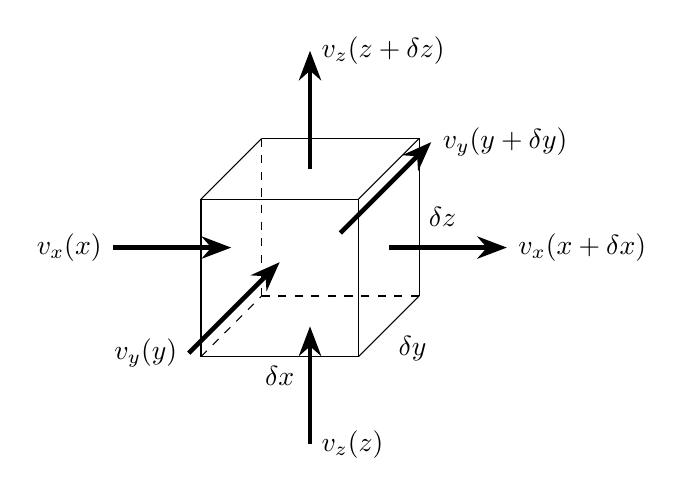
\begin{tikzpicture}[>=Stealth]
      \def\sliceZ{0.8}
      \def\side{2}
      \def\linewidth{0.6}
      \def\arrowlength{1.5}
      \draw[dashed] (\side,0,0) -- (0,0,0);
      \draw[dashed] (0,0,\side) -- (0,0,0);
      \draw[dashed] (0,\side,0) -- (0,0,0);
      \draw (\side,0,0) -- (\side,\side,0) node[midway,right]{$\delta z$} -- (0,\side,0);
      \draw (0,0,\side) -- (\side,0,\side) node[midway,below]{$\delta x$} -- (\side,\side,\side) -- (0,\side,\side) -- (0,0,\side);
      \draw (\side,0,0) -- (\side,0,\side) node[midway,below right]{$\delta y$};
      \draw (\side,\side,0) -- (\side,\side,\side);
      \draw (0,\side,0) -- (0,\side,\side);
      \node at (1,\sliceZ,1){};
      \draw[line width=\linewidth mm,<-](\side+\arrowlength,\side/2,\side/2) node[right]{$v_{x}(x+\delta x)$} -- (\side,\side/2,\side/2);
      \draw[line width=\linewidth mm,->](-\arrowlength,\side/2,\side/2) node[left]{$v_{x}(x)$} -- (0,\side/2,\side/2);
      \draw[line width=\linewidth mm,->](\side/2,\side/2+0.2,\side+3) node[left]{$v_{y}(y)$} -- (\side/2,\side/2+0.2,\side);
      \draw[line width=\linewidth mm,<-](\side/2,\side/2-0.2,-3) node[right]{$v_{y}(y+\delta y)$} -- (\side/2,\side/2-0.2,0);
      \draw[line width=\linewidth mm,<-](\side/2,\side+\arrowlength,\side/2) node[right]{$v_{z}(z+\delta z)$} -- (\side/2,\side,\side/2);
      \draw[line width=\linewidth mm,->](\side/2,-\arrowlength,\side/2) node[right]{$v_{z}(z)$} -- (\side/2,0,\side/2);
    \end{tikzpicture}
    \caption{Infinitesimal control volume}
  \end{center}
\end{figure}

The box is a fixed volume.
Continuity represents the rate of accumulation of mass within the box, minus the net flow out of the box.
Conservation of mass is written as

\begin{equation*}
  \begin{split}
    &\frac{\partial\rho}{\partial{}t}\delta x\delta y\delta z+\rho{}v_{x}(x)\delta y\delta z+\rho{}v_{y}(y)\delta x\delta z+\rho{}v_{z}(z)\delta x\delta y \\
    &=(\rho+\delta\rho_{x})v_{x}(x+\delta x)\delta y\delta z+(\rho+\delta\rho_{y})v_{y}(y+\delta y)\delta x\delta z+(\rho+\delta\rho_{z})v_{z}(z+\delta z)\delta x\delta y
  \end{split}
\end{equation*}
Note now that $\rho$ is a constant and thus all derivatives of $\rho$ are zero, giving

\begin{equation*}
  \begin{split}
    &v_{x}(x)\delta y\delta z+v_{y}(y)\delta x\delta z+v_{z}(z)\delta x\delta y \\
    &=v_{x}(x+\delta x)\delta y\delta z+v_{y}(y+\delta y)\delta x\delta z+v_{z}(z+\delta z)\delta x\delta y
  \end{split}
\end{equation*}
Multiplying each velocity term by unity gives

\begin{equation*}
  \begin{split}
    &v_{x}(x)\frac{\delta y\delta z\delta x}{\delta x}+v_{y}(y)\frac{\delta x\delta z\delta y}{\delta y}+v_{z}(z)\frac{\delta x\delta y\delta z}{\delta z} \\
    &=v_{x}(x+\delta x)\frac{\delta y\delta z\delta x}{\delta x}+v_{y}(y+\delta y)\frac{\delta x\delta z\delta y}{\delta y}+v_{z}(z+\delta z)\frac{\delta x\delta y\delta z}{\delta z}
  \end{split}
\end{equation*}
Dividing both sides by $\delta x\delta y\delta z$ gives

\begin{equation*}
  \frac{v_{x}(x)}{\delta x}+\frac{v_{y}(y)}{\delta y}+\frac{v_{z}(z)}{\delta z}=\frac{v_{x}(x+\delta x)}{\delta x}+\frac{v_{y}(y+\delta y)}{\delta y}+\frac{v_{z}(z+\delta z)}{\delta z}
\end{equation*}
Combining terms

\begin{equation*}
  \frac{v_{x}(x)-v_{x}(x+\delta x)}{\delta x}+\frac{v_{y}(y)-v_{y}(y+\delta y)}{\delta y}+\frac{v_{z}(z)-v_{z}(z+\delta z)}{\delta z}=0
\end{equation*}
Taking the limit as the fluid element gets small

\begin{equation*}
  \frac{\partial{}v_{x}}{\partial{}x}+\frac{\partial{}v_{y}}{\partial{}y}+\frac{\partial{}v_{z}}{\partial{}z}=0
\end{equation*}
In vector form

\begin{equation*}
  \begin{bmatrix}
    \frac{\partial}{\partial{}x} &
    \frac{\partial}{\partial{}y} &
    \frac{\partial}{\partial{}z}
  \end{bmatrix}
  \cdot
  \begin{bmatrix}
    v_{x} &
    v_{y} &
    v_{z}
  \end{bmatrix}
  =0
\end{equation*}
And of course this can be written using the del operator as

\begin{empheq}[box=\fboxTwo]{alignat*=3}
  &\mbox{\textbf{Incompressible mass conservation (differential):}} \hspace{0.5in}& \underline{\nabla}\cdot\underline{v}=0
\end{empheq}

\subsection{Conservation of Mass for a Compressible Fluid}

This section provides a control volume derivation of conservation of mass for a compressible fluid.
It follows the same derivation as the one above for incompressible fluids, except that the density is not constant and thus has, in general, nonzero derivatives.
Furthermore, the result above can be obtained from the one below when density is constant.

\begin{figure}[H]
  \begin{center}
    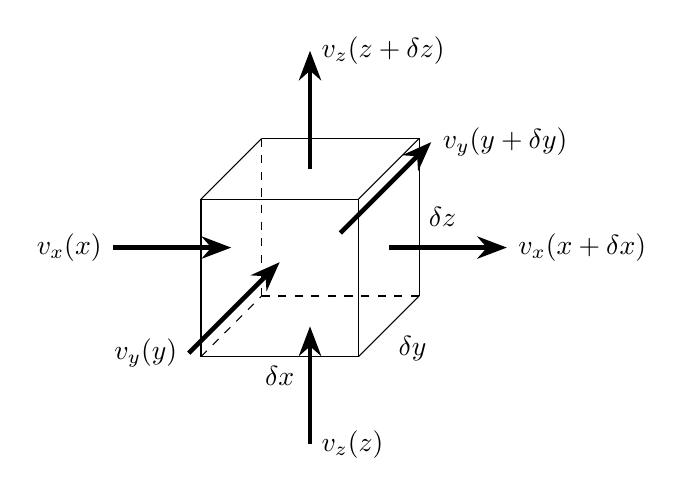
\begin{tikzpicture}[>=Stealth]
      \def\sliceZ{0.8}
      \def\side{2}
      \def\linewidth{0.6}
      \def\arrowlength{1.5}
      \draw[dashed] (\side,0,0) -- (0,0,0);
      \draw[dashed] (0,0,\side) -- (0,0,0);
      \draw[dashed] (0,\side,0) -- (0,0,0);
      \draw (\side,0,0) -- (\side,\side,0) node[midway,right]{$\delta z$} -- (0,\side,0);
      \draw (0,0,\side) -- (\side,0,\side) node[midway,below]{$\delta x$} -- (\side,\side,\side) -- (0,\side,\side) -- (0,0,\side);
      \draw (\side,0,0) -- (\side,0,\side) node[midway,below right]{$\delta y$};
      \draw (\side,\side,0) -- (\side,\side,\side);
      \draw (0,\side,0) -- (0,\side,\side);
      \node at (1,\sliceZ,1){};
      \draw[line width=\linewidth mm,<-](\side+\arrowlength,\side/2,\side/2) node[right]{$v_{x}(x+\delta x)$} -- (\side,\side/2,\side/2);
      \draw[line width=\linewidth mm,->](-\arrowlength,\side/2,\side/2) node[left]{$v_{x}(x)$} -- (0,\side/2,\side/2);
      \draw[line width=\linewidth mm,->](\side/2,\side/2+0.2,\side+3) node[left]{$v_{y}(y)$} -- (\side/2,\side/2+0.2,\side);
      \draw[line width=\linewidth mm,<-](\side/2,\side/2-0.2,-3) node[right]{$v_{y}(y+\delta y)$} -- (\side/2,\side/2-0.2,0);
      \draw[line width=\linewidth mm,<-](\side/2,\side+\arrowlength,\side/2) node[right]{$v_{z}(z+\delta z)$} -- (\side/2,\side,\side/2);
      \draw[line width=\linewidth mm,->](\side/2,-\arrowlength,\side/2) node[right]{$v_{z}(z)$} -- (\side/2,0,\side/2);
    \end{tikzpicture}
    \caption{Infinitesimal control volume}
  \end{center}
\end{figure}

Conservation of mass

\begin{equation*}
  \begin{split}
    &\frac{\partial\rho}{\partial{}t}\delta x\delta y\delta z+\rho{}v_{x}(x)\delta y\delta z+\rho{}v_{y}(y)\delta x\delta z+\rho{}v_{z}(z)\delta x\delta y \\
    &=(\rho+\delta\rho_{x})v_{x}(x+\delta x)\delta y\delta z+(\rho+\delta\rho_{y})v_{y}(y+\delta y)\delta x\delta z+(\rho+\delta\rho_{z})v_{z}(z+\delta z)\delta x\delta y
  \end{split}
\end{equation*}
Looking at the terms on the right hand side with

\begin{equation*}
  \delta\rho_{x}=\frac{\partial\rho}{\partial{}x}\delta x
  \hspace{0.5in}
  \delta\rho_{y}=\frac{\partial\rho}{\partial{}y}\delta y
  \hspace{0.5in}
  \delta\rho_{z}=\frac{\partial\rho}{\partial{}z}\delta z
\end{equation*}
and using a first order Taylor series approximation on the following

\begin{equation*}
  v_{x}(x+\delta x)=v_{x}(x)+\frac{\partial{}v_{x}}{\partial{}x}\delta x
\end{equation*}

\begin{equation*}
  v_{y}(y+\delta y)=v_{y}(y)+\frac{\partial{}v_{y}}{\partial{}y}\delta y
\end{equation*}

\begin{equation*}
  v_{z}(z+\delta z)=v_{z}(z)+\frac{\partial{}v_{z}}{\partial{}z}\delta z
\end{equation*}
we get

\begin{equation*}
  \begin{split}
  \rho{}v_{x}(x)\delta y\delta z+\rho{}v_{y}(y)\delta x\delta z+\rho{}v_{z}(z)\delta x\delta y
  &=\left(\rho+\frac{\partial\rho}{\partial{}x}\delta x\right)\left(v_{x}(x)+\frac{\partial{}v_{x}}{\partial{}x}\delta x\right)\delta y\delta z \\
  &+\left(\rho+\frac{\partial\rho}{\partial{}y}\delta y\right)\left(v_{y}(y)+\frac{\partial{}v_{y}}{\partial{}y}\delta y\right)\delta x\delta z \\
  &+\left(\rho+\frac{\partial\rho}{\partial{}z}\delta z\right)\left(v_{z}(z)+\frac{\partial{}v_{z}}{\partial{}z}\delta z\right)\delta x\delta y \\
  \end{split}
\end{equation*}
Multiplying out the left hand side and neglecting second order terms

\begin{equation*}
  \rho{}v_{x}(x)\delta y\delta z=
  \left(\rho{}v_{x}(x)+\rho\frac{\partial{}v_{x}}{\partial{}x}\delta x+v_{x}(x)\frac{\partial\rho}{\partial{}x}\delta x\right)\delta y\delta z
\end{equation*}

\begin{equation*}
  \rho{}v_{y}(y)\delta x\delta z=
  \left(\rho{}v_{y}(y)+\rho\frac{\partial{}v_{y}}{\partial{}y}\delta y+v_{y}(y)\frac{\partial\rho}{\partial{}y}\delta y\right)\delta x\delta z
\end{equation*}

\begin{equation*}
  \rho{}v_{z}(z)\delta x\delta y=
  \left(\rho{}v_{z}(z)+\rho\frac{\partial{}v_{z}}{\partial{}z}\delta z+v_{z}(z)\frac{\partial\rho}{\partial{}z}\delta z\right)\delta x\delta y
\end{equation*}
simplifying

\begin{equation*}
  0=\left(\rho\frac{\partial{}v_{x}}{\partial{}x}\delta x+v_{x}(x)\frac{\partial\rho}{\partial{}x}\delta x\right)\delta y\delta z
\end{equation*}

\begin{equation*}
  0=\left(\rho\frac{\partial{}v_{y}}{\partial{}y}\delta y+v_{y}(y)\frac{\partial\rho}{\partial{}y}\delta y\right)\delta x\delta z
\end{equation*}

\begin{equation*}
  0=\left(\rho\frac{\partial{}v_{z}}{\partial{}z}\delta z+v_{z}(z)\frac{\partial\rho}{\partial{}z}\delta z\right)\delta x\delta y
\end{equation*}
Recognizing these quantities as from product rule, and combining the components back onto a single equation

\begin{equation*}
  0=\frac{\partial(\rho{}v_{x})}{\partial{}x}\delta x+\frac{\partial(\rho{}v_{y})}{\partial{}y}\delta y+\frac{\partial(\rho{}v_{z})}{\partial{}z}\delta z
\end{equation*}
\begin{equation*}
  0=\frac{\partial(\rho{}v_{x})}{\partial{}x}+\frac{\partial(\rho{}v_{y})}{\partial{}y}+\frac{\partial(\rho{}v_{z})}{\partial{}z}
\end{equation*}
In vector form

\begin{equation*}
  \frac{\partial\rho}{\partial{}t}+
  \begin{bmatrix}
    \frac{\partial}{\partial{}x} &
    \frac{\partial}{\partial{}y} &
    \frac{\partial}{\partial{}z}
  \end{bmatrix}
  \cdot
  \begin{bmatrix}
    \rho{}v_{x} &
    \rho{}v_{y} &
    \rho{}v_{z}
  \end{bmatrix}
  =0
\end{equation*}
And again this can be written as follows using the del operator.

\begin{empheq}[box=\fboxTwo]{alignat*=3}
  &\mbox{\textbf{Compressible mass conservation (differential):}} \hspace{0.5in}& \frac{\partial\rho}{\partial{}t}+\underline{\nabla}\cdot(\rho\underline{v})=0
\end{empheq}
And we can see that if $\rho$ is a constant, this expression reduces to conservation of mass for an incompressible fluid.

\section{Conservation of Momentum}

\subsection{Cauchy Momentum Equation}

This is the most basic form, where the surface and pressure forces are very general.
Fluid doesn't have to be Newtonian, or compressible, etc.

\subsection{Conservation of Momentum with Euler's Equation}

This section is about conservation of momentum for an incompressible fluid with pressure and gravity, deriving Euler's Equation.

Conservation of momentum when only surface force is pressure and only body force is gravity.
Consider a differential element of fluid, and consider only pressure and gravity forces acting upon it.
We also assume the density is constant.
To derive Euler's equation, by assuming that these are the only forces acting on the fluid, this version of Euler's equation is only valid for inviscid, incompressible flows.

\begin{figure}[H]
  \begin{center}
    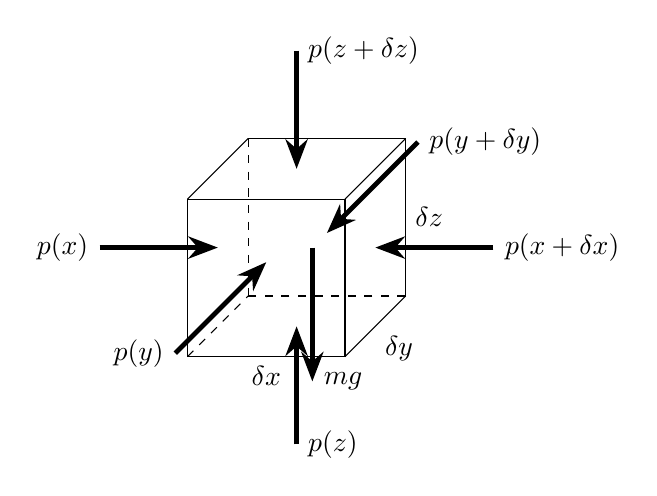
\begin{tikzpicture}[>=Stealth]
      \def\sliceZ{0.8}
      \def\side{2}
      \def\linewidth{0.6}
      \def\arrowlength{1.5}
      \draw[dashed] (\side,0,0) -- (0,0,0);
      \draw[dashed] (0,0,\side) -- (0,0,0);
      \draw[dashed] (0,\side,0) -- (0,0,0);
      \draw (\side,0,0) -- (\side,\side,0) node[midway,right]{$\delta z$} -- (0,\side,0);
      \draw (0,0,\side) -- (\side,0,\side) node[midway,below]{$\delta x$} -- (\side,\side,\side) -- (0,\side,\side) -- (0,0,\side);
      \draw (\side,0,0) -- (\side,0,\side) node[midway,below right]{$\delta y$};
      \draw (\side,\side,0) -- (\side,\side,\side);
      \draw (0,\side,0) -- (0,\side,\side);
      \node at (1,\sliceZ,1){};
      \draw[line width=\linewidth mm,->](\side+\arrowlength,\side/2,\side/2) node[right]{$p(x+\delta x)$} -- (\side,\side/2,\side/2);
      \draw[line width=\linewidth mm,->](-\arrowlength,\side/2,\side/2) node[left]{$p(x)$} -- (0,\side/2,\side/2);
      \draw[line width=\linewidth mm,->](\side/2,\side/2+0.2,\side+3) node[left]{$p(y)$} -- (\side/2,\side/2+0.2,\side);
      \draw[line width=\linewidth mm,->](\side/2,\side/2-0.2,-3) node[right]{$p(y+\delta y)$} -- (\side/2,\side/2-0.2,0);
      \draw[line width=\linewidth mm,->](\side/2,\side+\arrowlength,\side/2) node[right]{$p(z+\delta z)$} -- (\side/2,\side,\side/2);
      \draw[line width=\linewidth mm,->](\side/2,-\arrowlength,\side/2) node[right]{$p(z)$} -- (\side/2,0,\side/2);
      \draw[line width=\linewidth mm,->](\side/2+0.2,\side/2,\side/2) -- (\side/2+0.2,\side/2-\arrowlength-0.2,\side/2) node[right]{$mg$};
    \end{tikzpicture}
    \caption{Fluid element with pressure and gravity acting on it}
  \end{center}
\end{figure}

Summing the forces in the $x$, $y$, and $z$ directions we have

\begin{equation*}
  \begin{split}
    p\delta y\delta z-\left(p+\frac{\partial{}p}{\partial{}x}\right)\delta y\delta z&=\rho\delta x\delta y\delta za_{x} \\
    p\delta x\delta z-\left(p+\frac{\partial{}p}{\partial{}y}\right)\delta x\delta z&=\rho\delta x\delta y\delta za_{y} \\
    p\delta x\delta y-\left(p+\frac{\partial{}p}{\partial{}z}\right)\delta x\delta y-\rho{}g_{z}\delta x\delta y\delta z&=\rho\delta x\delta y\delta za_{z} \\
  \end{split}
\end{equation*}

simplifying

\begin{equation*}
  \begin{split}
    -\frac{\partial{}p}{\partial{}x}&=\rho{}a_{x} \\
    -\frac{\partial{}p}{\partial{}y}&=\rho{}a_{y} \\
    -\frac{\partial{}p}{\partial{}z}-\rho{}g_{z}&=\rho{}a_{z}
  \end{split}
\end{equation*}

we obtain

\begin{empheq}[box=\roomyfbox]{equation*}
  \rho\underline{a}=-\underline{\nabla}p+\rho\underline{g}
\end{empheq}

Substituting the following

\begin{equation*}
  \begin{split}
    \underline{a}&=\frac{D\underline{v}}{Dt} \\
    &=\frac{\partial\underline{v}}{\partial{}t}+(\underline{v}\cdot\underline{\nabla})\underline{v}
  \end{split}
\end{equation*}

into above to obtain

\begin{empheq}[box=\fboxTwo]{alignat=3}
  &\mbox{\textbf{Euler's Equation:}} \hspace{0.5in} &\rho\left(\frac{\partial\underline{v}}{\partial{}t}+ (\underline{v}\cdot\underline{\nabla})\underline{v}\right)=-\underline{\nabla}p+\rho\underline{g}\label{eqn.fluids.eulers-equation}
\end{empheq}

The assumptions of Euler's equation are: inviscid flow (neglects stress tensor $\uuline{\tau}$).
For inviscid flow, if it is irrotational at any instant in time, it remains irrotational for all subsequent time.

\subsection{Conservation of Momentum including Viscous Forces}

The above derivation can be repeated including surface forces (but still assuming density is constant), resulting in the following.

\begin{empheq}[box=\roomyfbox]{equation*}
  \rho\left(\frac{\partial\underline{v}}{\partial{}t}+\underline{\nabla}\cdot(\underline{v}\underline{v})\right)=-\underline{\nabla}p+\underline{\nabla}\cdot\tau+\rho\underline{g}
\end{empheq}

\chapter{Material Derivative}

Local change plus convective change, where $\underline{f}$ can be a vector or scalar quantity.
The left hand side of the equation is the Lagrangian side: it is following a particular material element through the flow, and the right hand side is the Eulerian side.

\begin{empheq}[box=\fboxTwo]{alignat*=3}
  &\mbox{\textbf{Material Derivative:}} &\hspace{0.5in} \frac{D\underline{f}}{Dt}=\underbrace{\frac{\partial\underline{f}}{\partial{}t}}_{\text{local rate of change}}+\underbrace{\underline{f}\cdot\underline{\nabla}\;\underline{f}}_{\text{convective change}}
\end{empheq}

\section{Hydrostatics}

Note that in hydrostatic problems the fluid is at rest, and so viscosity can be ignored, we set $\underline{a}=0$ in Euler's equation to obtain the following

\begin{empheq}[box=\fboxTwo]{alignat*=3}
  &\mbox{\textbf{Hydrostatic Equation:}} &\hspace{0.5in} \underline{\nabla}p=\rho\underline{g}
\end{empheq}
In a lot of cases, pressure variations occur only in the vertical direction due to gravity.
In these cases we have
\begin{equation*}
  \begin{split}
    \underline{\nabla}p&=\rho\underline{g} \\
    \begin{bmatrix}
      \frac{\partial{}p}{\partial{}x} & \frac{\partial{}p}{\partial{}y}& \frac{\partial{}p}{\partial{}z}
    \end{bmatrix}&=
    \rho
    \begin{bmatrix}
      g_{x} & g_{y} & g_{z}
    \end{bmatrix}
  \end{split}
\end{equation*}
If we have a coordinate system where the $z$ axis points upwards and gravity points downwards, the $z$ component of gravity is $g_{z}=-g$ where $g$ is gravitational acceleration constant, e.g.\ $9.81$ m/s$^{2}$ on Earth.
This gives
\begin{equation*}
  \frac{\partial{}p}{\partial{}z}=-\rho{}g
\end{equation*}
Separating and integrating back
\begin{equation*}
  \begin{split}
    \int\partial{}p&=-\int\rho{}g\partial{}z \\
    p_{2}-p_{1}&=-\rho{}g(z_{2}-z_{1})
  \end{split}
\end{equation*}

\subsection{Force and Moment}
To find force and moment about a point on say, a door or floodgate holding back hydrostatic fluid

\begin{equation*}
  F=\int_{A}p(z)dA
\end{equation*}

\begin{equation*}
  \tau=\int_{A}rp(z)dA
\end{equation*}

where $r$ is the distance from the point about which we are taking moments along the door or floodgate.

\section{Motion of a Fluid Element Along a Streamline}

\subsection{Streamline Coordinates}

The $osnl$ coordinate is orthogonal but not always Cartesian.
For example for the rigid body problem streamlines are circles and the $osnl$ coordinate system becomes similar to cylindrical ($e_{s}$ is $e_{\theta}$ and $e_{n}$ is $e_{r}$ and $e_{l}$ is $e_{z}$) whereas in other arbitrary flows it may be something else.
What people call these is a subset of ``curvilinear coordiante systems'' See Wikipedia.

% TODO@dpwiese
Assume constant density?
Think about looking at Euler's equation along a streamline in order to simplify it.
This will allow the velocity components to be simplified, since by definition the velocity vector along a streamline is always tangent to the streamline.
Recall Euler's equation in\ \eqref{eqn.fluids.eulers-equation}.

Start generally though with with the velocity vector given by the following components
\begin{equation*}
  \underline{v}=
  v_{s}\hat{\underline{e}}_{s}+v_{n}\;\hat{\underline{e}}_{n}+v_{l}\;\hat{\underline{e}}_{l}=
  \begin{bmatrix}
    v_{s} \\
    v_{n} \\
    v_{l}
  \end{bmatrix}
\end{equation*}
Evaluating Euler's equation starting with the term $\underline{v}\cdot\underline{\nabla}$
\begin{equation*}
  \underline{v}\cdot\underline{\nabla}=
  \begin{bmatrix}
    v_{s} \\
    v_{n} \\
    v_{l}
  \end{bmatrix}
  \cdot
  \begin{bmatrix}
    \frac{\partial}{\partial{}s} \\
    \frac{\partial}{\partial{}n} \\
    \frac{\partial}{\partial{}l}
  \end{bmatrix}=
  v_{s}\frac{\partial}{\partial{}s}+
  v_{n}\frac{\partial}{\partial{}n}+
  v_{l}\frac{\partial}{\partial{}l}
\end{equation*}
Now evaluating $(\underline{v}\cdot\underline{\nabla})\underline{v}$
\begin{equation*}
  \begin{split}
    (\underline{v}\cdot\underline{\nabla})\underline{v}&=
    \left(v_{s}\frac{\partial}{\partial{}s}+
    v_{n}\frac{\partial}{\partial{}n}+
    v_{l}\frac{\partial}{\partial{}l}\right)\underline{v} \\
    &=v_{s}\frac{\partial}{\partial{}s}\underline{v}+
    v_{n}\frac{\partial}{\partial{}n}\underline{v}+
    v_{l}\frac{\partial}{\partial{}l}\underline{v} \\
    &=v_{s}\frac{\partial}{\partial{}s}(v_{s}\hat{\underline{e}}_{s}+v_{n}\;\hat{\underline{e}}_{n}+v_{l}\;\hat{\underline{e}}_{l}) \\
    &\qquad+v_{n}\frac{\partial}{\partial{}n}(v_{s}\hat{\underline{e}}_{s}+v_{n}\;\hat{\underline{e}}_{n}+v_{l}\;\hat{\underline{e}}_{l}) \\
    &\qquad+v_{l}\frac{\partial}{\partial{}l}(v_{s}\hat{\underline{e}}_{s}+v_{n}\;\hat{\underline{e}}_{n}+v_{l}\;\hat{\underline{e}}_{l}) \\
    &=v_{s}\frac{\partial}{\partial{}s}(v_{s}\hat{\underline{e}}_{s})+v_{n}\frac{\partial}{\partial{}n}(v_{s}\hat{\underline{e}}_{s})+
    v_{l}\frac{\partial}{\partial{}l}(v_{s}\hat{\underline{e}}_{s}) \\
    &\qquad+v_{s}\frac{\partial}{\partial{}s}(v_{n}\hat{\underline{e}}_{n})+v_{n}\frac{\partial}{\partial{}n}(v_{n}\hat{\underline{e}}_{n})+
    v_{l}\frac{\partial}{\partial{}l}(v_{n}\hat{\underline{e}}_{n}) \\
    &\qquad+v_{s}\frac{\partial}{\partial{}s}(v_{l}\hat{\underline{e}}_{l})+v_{n}\frac{\partial}{\partial{}n}(v_{l}\hat{\underline{e}}_{l})+
    v_{l}\frac{\partial}{\partial{}l}(v_{l}\hat{\underline{e}}_{l}) \\
  \end{split}
\end{equation*}

Now using the following simplification since we are considering flow along a streamline we have $v_{n}=v_{l}=0$.
Using this, we simplify the above to
\begin{equation*}
  \begin{split}
    (\underline{v}\cdot\underline{\nabla})\underline{v}
    &=v_{s}\frac{\partial}{\partial{}s}(v_{s}\hat{\underline{e}}_{s}) \\
    &=v_{s}\left(\frac{\partial}{\partial{}s}(v_{s})\hat{\underline{e}}_{s}+v_{s}\frac{\partial}{\partial{}s}(\hat{\underline{e}}_{s})\right)
  \end{split}
\end{equation*}
Since $\hat{\underline{e}}_{s}$ has unit magnitude, it can change only in direction.
This change must be perpendicular to $\hat{\underline{e}}_{s}$ itself.
Therefore $\hat{\underline{e}}_{n}$ is defined by
\begin{equation*}
  \hat{\underline{e}}_{n}=-R\frac{\partial\hat{\underline{e}}_{s}}{\partial{}s}
\end{equation*}
giving
\begin{equation*}
  \frac{\partial\hat{\underline{e}}_{s}}{\partial{}s}=-\frac{1}{R}\hat{\underline{e}}_{n}
\end{equation*}
\begin{equation*}
  (\underline{v}\cdot\underline{\nabla})\underline{v}
  =v_{s}\frac{\partial{}v_{s}}{\partial{}s}\hat{\underline{e}}_{s}-\frac{v_{s}^{2}}{R}\hat{\underline{e}}_{n}
\end{equation*}

\subsection{Motion Tangent to the Streamline}

We can see in this expression that there is a component of acceleration tangential to the streamline, as well as the centripetal component of acceleration.
If we neglect the centripetal acceleration, we have
\begin{empheq}[box=\roomyfbox]{equation*}
  (\underline{v}\cdot\underline{\nabla})\underline{v}=v_{s}\frac{\partial{}v_{s}}{\partial{}s}\hat{\underline{e}}_{s}
\end{empheq}
The next term we are looking at is $\frac{\partial\underline{v}}{\partial{}t}$ at a fixed point in space, and we are considering steady flow here, so
\begin{empheq}[box=\roomyfbox]{equation*}
  \frac{\partial\underline{v}}{\partial{}t}=0
\end{empheq}
Looking at the terms on the right hand side we have
\begin{equation*}
  \underline{\nabla}p=\frac{\partial{}p}{\partial{}s}\hat{\underline{e}}_{s}+\frac{\partial{}p}{\partial{}n}\hat{\underline{e}}_{n}+\frac{\partial{}p}{\partial{}l}\hat{\underline{e}}_{l}
\end{equation*}
And if we consider only pressure variations along the streamline, this expression is simplified to
\begin{empheq}[box=\roomyfbox]{equation*}
  \underline{\nabla}p=\frac{\partial{}p}{\partial{}s}\hat{\underline{e}}_{s}
\end{empheq}
With $g$ a vector pointing down, and considering only the component of gravity along the streamline $g_{s}$ we have
\begin{empheq}[box=\roomyfbox]{equation*}
  \rho\underline{g}=\rho{}g_{s}\hat{\underline{e}}_{s}
\end{empheq}
And sothe total simplified Euler equation along a streamline as
\begin{equation*}
  \rho{}v_{s}\frac{\partial{}v_{s}}{\partial{}s}\hat{\underline{e}}_{s}=-\frac{\partial{}p}{\partial{}s}\hat{\underline{e}}_{s}+\rho{}g_{s}\hat{\underline{e}}_{s}
\end{equation*}
Dropping the unit vector showing its along the streamline
\begin{empheq}[box=\roomyfbox]{equation*}
  \rho{}v_{s}\frac{\partial{}v_{s}}{\partial{}s}=-\frac{\partial{}p}{\partial{}s}+\rho{}g_{s}
\end{empheq}

but we can express $g_{s}$ as

\begin{equation*}
g_{s}=-g\frac{dz}{ds}
\end{equation*}

giving

\begin{equation*}
  \rho{}v_{s}\frac{\partial{}v_{s}}{\partial{}s}=-\frac{\partial{}p}{\partial{}s}-\rho{}g\frac{dz}{ds}
\end{equation*}

moving stuff over

\begin{equation*}
  \rho{}v_{s}\frac{\partial{}v_{s}}{\partial{}s}+\frac{\partial{}p}{\partial{}s}+\rho{}g\frac{dz}{ds}=0
\end{equation*}

\begin{equation*}
  \rho{}v_{s}\partial{}v_{s}+\partial{}p+\rho{}gdz=0
\end{equation*}

\subsection{Bernoulli's Equation}

integrating, but only in the $s$-direction

\begin{equation*}
  \int_{s_{1}}^{s_{2}}\left(\rho{}v_{s}\frac{\partial{}v_{s}}{\partial{}s}+\frac{\partial{}p}{\partial{}s}+\rho{}g\frac{dz}{ds}\right)=0
\end{equation*}

\begin{equation*}
  \int_{s_{1}}^{s_{2}}(\rho{}v_{s}\partial{}v_{s}+\partial{}p+\rho{}gdz)=0
\end{equation*}

\begin{equation*}
  \frac{1}{2}\rho{}v_{s}^{2}(s)+p(s)+\rho{}gz(s)\biggr|_{s_{1}}^{s_{2}}=0
\end{equation*}

\begin{equation*}
  \left(\frac{1}{2}\rho{}v_{s}^{2}(s_{2})+p(s_{2})+\rho{}gz(s_{2})\right)-\left(\frac{1}{2}\rho{}v_{s}^{2}(s_{1})+p(s_{1})+\rho{}gz(s_{1})\right)=0
\end{equation*}

finally

\begin{empheq}[box=\fboxTwo]{alignat*=3}
  &\mbox{\textbf{Bernoulli's along streamline:}} &\hspace{0.5in} \frac{1}{2}\rho{}v_{s2}^{2}+p_{2}+\rho{}gz_{2}=\frac{1}{2}\rho{}v_{s1}^{2}+p_{1}+\rho{}gz_{1}
\end{empheq}

Bernoulli's equation is for steady incompressible flow of a fluid in the absence of viscous effects along a streamline.

\subsection{Motion Normal to the Streamline}

\begin{empheq}[box=\roomyfbox]{equation*}
  (\underline{v}\cdot\underline{\nabla})\underline{v}=\frac{v_{s}^{2}}{R}\hat{\underline{e}}_{n}
\end{empheq}
The next term we are looking at is $\frac{\partial\underline{v}}{\partial{}t}$ at a fixed point in space, and we are considering steady flow here, so
\begin{empheq}[box=\roomyfbox]{equation*}
  \frac{\partial\underline{v}}{\partial{}t}=0
\end{empheq}
Looking at the terms on the right hand side we have
\begin{equation*}
  \underline{\nabla}p=\frac{\partial{}p}{\partial{}s}\hat{\underline{e}}_{s}+\frac{\partial{}p}{\partial{}n}\hat{\underline{e}}_{n}+\frac{\partial{}p}{\partial{}l}\hat{\underline{e}}_{l}
\end{equation*}
And if we consider only pressure variations normal to the streamline, this expression is simplified to
\begin{empheq}[box=\roomyfbox]{equation*}
  \underline{\nabla}p=\frac{\partial{}p}{\partial{}n}\hat{\underline{e}}_{n}
\end{empheq}
With $g$ a vector pointing down, and considering only the component of gravity along the streamline $g_{s}$ we have
\begin{empheq}[box=\roomyfbox]{equation*}
  \rho\underline{g}=\rho{}g_{n}\hat{\underline{e}}_{n}
\end{empheq}
And sothe total simplified Euler equation along a streamline as

\begin{equation*}
  -\rho\frac{v_{s}^{2}}{R}\hat{\underline{e}}_{n}=-\frac{\partial{}p}{\partial{}n}\hat{\underline{e}}_{n}+\rho{}g_{n}\hat{\underline{e}}_{n}
\end{equation*}

\begin{empheq}[box=\fboxTwo]{alignat*=3}
  &\mbox{\textbf{Bernoulli's equation normal to streamline:}} &\hspace{0.5in} -\rho\frac{v_{s}^{2}}{R}=-\frac{\partial{}p}{\partial{}n}+\rho{}g_{n}
\end{empheq}

From this expression we can see that the change in pressure with respect to the normal direction is always positive with respect to $R$, so pressure increases in the $n$ direction.

\section{Solid Body Rotation}

Rotating bucket of water.
The velocity is dependent only on the radial direction $r$.
This cylindrical coordinate system is inertially fixed.
Bucket spinning with angular velocity $\Omega$.

\begin{figure}[H]
  \begin{center}
    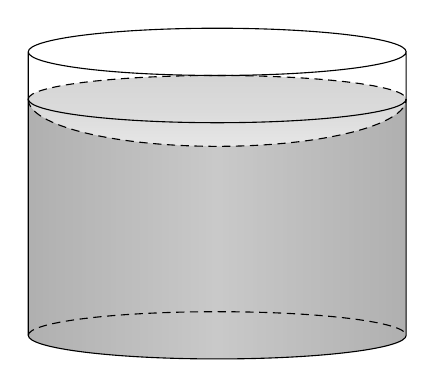
\begin{tikzpicture}[scale=0.6]
      \fill[top color=gray!50!black,bottom color=gray!10,middle color=gray,shading=axis,opacity=0.10] (-4,5) -- (4,5) arc (360:180:4cm and 1cm) -- (-4,5) -- (4,5) arc (360:180:4cm and -0.5cm);
      \fill[left color=gray!50!black,right color=gray!50!black,middle color=gray!50,shading=axis,opacity=0.20] (4,0) -- (4,5) arc (360:180:4cm and 1cm) -- (-4,0) arc (180:360:4cm and 0.5cm);
      \draw (-4,6) -- (-4,0) arc (180:360:4cm and 0.5cm) -- (4,6) ++ (-4,0) circle (4cm and 0.5cm);
      \draw[densely dashed] (-4,0) arc (180:0:4cm and 0.5cm);
      \draw[densely dashed] (-4,5) arc (180:0:4cm and 0.5cm);
      \draw[densely dashed] (-4,5) arc (180:0:4cm and -1cm);
      \draw (-4,5) -- (-4,5) arc (180:360:4cm and 0.5cm);
    \end{tikzpicture}
    \caption{Solid body rotation}
  \end{center}
\end{figure}

Thus, the total velocity in cylindrical coordinates is

\begin{equation*}
  \underline{v}=
  v_{r}\hat{\underline{e}}_{r}+v_{\theta}\hat{\underline{e}}_{\theta}+v_{z}\hat{\underline{e}}_{z}=
  \begin{bmatrix}
    v_{r} \\
    v_{\theta} \\
    v_{z}
  \end{bmatrix}=
  \begin{bmatrix}
    0 \\
    r\Omega \\
    0
  \end{bmatrix}
\end{equation*}

Apply Euler's equation

\begin{equation*}
  \rho\underline{a}=-\underline{\nabla}p+\rho\underline{g}
\end{equation*}

\begin{equation*}
  \underline{a}=\frac{D\underline{v}}{Dt}=\frac{\partial\underline{v}}{\partial{}t}+\underline{v}\cdot\underline{\nabla}\;\underline{v}
\end{equation*}

\subsection{Cylindrical Coordinates}

The partial derivative with respect to time, also known as the local rate of change, is zero, because at a fixed point in the fluid, the velocity is not changing with time.

\begin{equation*}
  \frac{\partial\underline{v}}{\partial{}t}=0
\end{equation*}
Looking at the next term

\begin{equation*}
  \underline{\nabla}=\frac{\partial}{\partial{}r}\hat{\underline{e}}_{r}+\frac{1}{r}\frac{\partial}{\partial\theta}\hat{\underline{e}}_{\theta}+\frac{\partial}{\partial{}z}\hat{\underline{e}}_{z}
\end{equation*}
Now evaluating $(\underline{v}\cdot\underline{\nabla})\underline{v}$

\begin{equation*}
  \begin{split}
    (\underline{v}\cdot\underline{\nabla})\underline{v}&=
    \left(v_{r}\frac{\partial}{\partial{}r}+
    \frac{1}{r}v_{\theta}\frac{\partial}{\partial\theta}+
    v_{z}\frac{\partial}{\partial{}z}\right)\underline{v} \\
    &=v_{r}\frac{\partial}{\partial{}r}\underline{v}+
    \frac{1}{r}v_{\theta}\frac{\partial}{\partial\theta}\underline{v}+
    v_{z}\frac{\partial}{\partial{}z}\underline{v} \\
    &=v_{r}\frac{\partial}{\partial{}r}(v_{r}\hat{\underline{e}}_{r}+v_{\theta}\;\hat{\underline{e}}_{\theta}+v_{z}\;\hat{\underline{e}}_{z}) \\
    &\qquad+\frac{1}{r}v_{\theta}\frac{\partial}{\partial\theta}(v_{r}\hat{\underline{e}}_{r}+v_{\theta}\;\hat{\underline{e}}_{\theta}+v_{z}\;\hat{\underline{e}}_{z}) \\
    &\qquad+v_{z}\frac{\partial}{\partial{}z}(v_{r}\hat{\underline{e}}_{r}+v_{\theta}\;\hat{\underline{e}}_{\theta}+v_{z}\;\hat{\underline{e}}_{z}) \\
  \end{split}
\end{equation*}
Now substitute in that $v_{r}=v_{z}=0$ and get

\begin{equation*}
  \begin{split}
    (\underline{v}\cdot\underline{\nabla})\;\underline{v}
    &=\frac{1}{r}v_{\theta}\frac{\partial}{\partial\theta}(v_{\theta}\hat{\underline{e}}_{\theta}) \\
    &=\frac{1}{r}v_{\theta}\frac{\partial{}v_{\theta}}{\partial\theta}\hat{\underline{e}}_{\theta}+\frac{1}{r}v_{\theta}^{2}\frac{\partial\hat{\underline{e}}_{\theta}}{\partial\theta} \\
    &=0+\frac{1}{r}v_{\theta}^{2}\frac{\partial\hat{\underline{e}}_{\theta}}{\partial\theta} \\
    &=-\frac{v_{\theta}^{2}}{r}\hat{\underline{e}}_{r}
  \end{split}
\end{equation*}
since

\begin{equation*}
  \frac{\partial\hat{\underline{e}}_{\theta}}{\partial\theta}=-\hat{\underline{e}}_{r}
\end{equation*}
And note that we have

\begin{equation*}
  \underline{a}=\frac{D\underline{v}}{Dt}=-\frac{v_{\theta}^{2}}{r}\hat{\underline{e}}_{r}
\end{equation*}
So we can see this as centripetal acceleration.
The surface force term

\begin{equation*}
  \underline{\nabla}p=\frac{\partial{}p}{\partial{}r}\hat{\underline{e}}_{r}+\frac{1}{r}\frac{\partial{}p}{\partial\theta}\hat{\underline{e}}_{\theta}+\frac{\partial{}p}{\partial{}z}\hat{\underline{e}}_{z}
\end{equation*}
body force term

\begin{equation*}
  \rho\underline{g}=-\rho{}g_{z}\hat{\underline{e}}_{z}
\end{equation*}
Forming the whole equation we have

\begin{equation*}
  -\rho\frac{v_{\theta}^{2}}{r}\hat{\underline{e}}_{r}=-\frac{\partial{}p}{\partial{}r}\hat{\underline{e}}_{r}-\frac{1}{r}\frac{\partial{}p}{\partial\theta}\hat{\underline{e}}_{\theta}-\frac{\partial{}p}{\partial{}z}\hat{\underline{e}}_{z}-\rho{}g_{z}\hat{\underline{e}}_{z}
\end{equation*}
Equating the components we have

\begin{equation*}
  -\rho\frac{v_{\theta}^{2}}{r}=-\frac{\partial{}p}{\partial{}r}
  \hspace{0.5in}
  0=-\frac{1}{r}\frac{\partial{}p}{\partial\theta}
  \hspace{0.5in}
  0=-\frac{\partial{}p}{\partial{}z}-\rho{}g_{z}
\end{equation*}
This gives

\begin{equation*}
  \frac{\partial{}p}{\partial{}r}=\rho{}r\Omega^{2}
  \hspace{0.5in}
  \frac{\partial{}p}{\partial\theta}=0
  \hspace{0.5in}
  \frac{\partial{}p}{\partial{}z}=-\rho{}g_{z}
\end{equation*}
separating and integrating these back

\begin{equation*}
  \int\partial{}p=\int\rho{}r\Omega^{2}\partial{}r
  \hspace{0.5in}
  \frac{\partial{}p}{\partial\theta}=0
  \hspace{0.5in}
  \int\partial{}p=-\int\rho{}g_{z}\partial{}z
\end{equation*}
The second equation shows that the pressure is not a function of $\theta$.
Integrating back the first and third equations we have the following

\begin{equation*}
  \begin{split}
    p&=\frac{1}{2}\rho{}r^{2}\Omega^{2}+f(z)+c \\
    p&=-\rho{}g_{z}z+g(r)+c
  \end{split}
\end{equation*}
and we have

\begin{equation*}
  \begin{split}
    f(z)&=-\rho{}g_{z}z \\
    g(r)&=\frac{1}{2}\rho{}r^{2}\Omega^{2}
  \end{split}
\end{equation*}
and so the pressure in the rotating cylinder is given by

\begin{equation*}
  p(r,z)=\frac{1}{2}\rho{}r^{2}\Omega^{2}-\rho{}g_{z}z+c
\end{equation*}
And we can find the constant $c$ by setting $r=0$ and looking at the interface height at the center of the cylinder, at the vertex of the parabaloid shape, and call this height $z_{0}$.
At this point, the pressure is equal to atmospheric pressure.

\begin{equation*}
  p(r=0,z_{0})=-\rho{}g_{z}z_{0}+c=p_{\text{atm}}
\end{equation*}
giving the following value of the constant

\begin{equation*}
  c=\rho{}g_{z}z_{0}+p_{\text{atm}}
\end{equation*}
substituting this into the pressure equation we obtain the following

\begin{empheq}[box=\fboxTwo]{alignat*=3}
  &\mbox{\textbf{Pressure for solid body rotation:}} &\hspace{0.5in} p(r,z)=\frac{1}{2}\rho{}r^{2}\Omega^{2}+\rho{}g_{z}(z_{0}-z)+p_{\text{atm}}
\end{empheq}
To determine the shape that the air-water interface makes, we apply the boundary condition at this interface.
That is

\begin{equation*}
  p(r,z)\bigr|_{\text{interface}}=p_{\text{atm}}
\end{equation*}
And then we have

\begin{equation*}
  0=\frac{1}{2}\rho{}r_{\text{interface}}^{2}\Omega^{2}-\rho{}g_{z}z_{\text{interface}}+\rho{}g_{z}z_{0}
\end{equation*}

\begin{equation*}
  z_{\text{interface}}=\frac{\Omega^{2}}{2g_{z}}r_{\text{interface}}^{2}+z_{0}
\end{equation*}

\subsubsection{Isobars}

Can also find out the shape of the fluid by solving for isobars by evaluating $dp$ and setting it equal to zero.
Since $p=p(r,z)$ chain rule gives us the following for $dp$.

\begin{equation*}
  dp=\left(\frac{\partial{}p}{\partial{}r}\right)dr+\left(\frac{\partial{}p}{\partial{}z}\right)dz
\end{equation*}
\begin{equation*}
  dp=\rho{}r\Omega^{2}dr-\rho{}g_{z}dz=0
\end{equation*}
\begin{equation*}
  g_{z}dz=r\Omega^{2}dr
\end{equation*}
Integrating back and solving for the constant of integration when $r=0$ we have
\begin{equation*}
  z=\frac{\Omega^{2}}{2g_{z}}r^{2}+h_{0}
\end{equation*}

\subsubsection{Vorticity}

The vorticity of a fluid element in our bucket is given by the curl of the velocity vector.
That is,

\begin{equation*}
  \begin{split}
    \underline{\omega}&=\underline{\nabla}\times\underline{v} \\
    &=\left(\hat{\underline{e}}_{r}\frac{\partial}{\partial{}r}+\hat{\underline{e}}_{\theta}\frac{1}{r}\frac{\partial}{\partial{}r}+\hat{\underline{e}}_{z}\frac{\partial}{\partial{}z}\right)\times\left(0\hat{\underline{e}}_{r}+r\Omega\hat{\underline{e}}_{\theta}+0\hat{\underline{e}}_{z}\right) \\
    &=\hat{\underline{e}}_{r}\times\frac{\partial}{\partial{}r}(r\Omega\hat{\underline{e}}_{\theta})+
    \hat{\underline{e}}_{\theta}\frac{1}{r}\times\frac{\partial}{\partial\theta}(r\Omega\hat{\underline{e}}_{\theta})+
    \hat{\underline{e}}_{z}\times\frac{\partial}{\partial{}z}(r\Omega\hat{\underline{e}}_{\theta}) \\
    &=\hat{\underline{e}}_{r}\times(\Omega\hat{\underline{e}}_{\theta})+\hat{\underline{e}}_{\theta}\frac{1}{r}\times(-r\Omega\hat{\underline{e}}_{r}) \\
    &=2\Omega\hat{\underline{e}}_{z}
  \end{split}
\end{equation*}
And from this expression we can see that the vorticity everywhere in the fluid is the same.

\subsection{Cartesian Coordinates}
% TODO@dpwiese
Velocity is given in cylindrical coordinates, so we convert it to cartesian coordinates, using an inertially fixed coordinate system
\begin{equation*}
  \underline{v}=
  \begin{bmatrix}
    v_{r} \\
    v_{\theta} \\
    v_{z}
  \end{bmatrix}=
  \begin{bmatrix}
    0 \\
    r\omega \\
    0
  \end{bmatrix}
\end{equation*}

\begin{equation*}
  \begin{split}
    x&=r\cos{\theta} \\
    y&=r\sin{\theta}
  \end{split}
\end{equation*}

% \begin{figure}[H]
%   \begin{center}
%     \begin{tikzpicture}[
%       scale=5,
%       axis/.style={very thick, ->, >=stealth'},
%       important line/.style={thick},
%       dashed line/.style={dashed, thin},
%       pile/.style={thick, ->, >=stealth', shorten <=2pt, shorten
%       >=2pt},
%       every node/.style={color=black}
%       ]
%       % axis
%       \draw[axis] (-0.1,0)  -- (1.1,0) node(xline)[right]
%         {$G\uparrow/T\downarrow$};
%       \draw[axis] (0,-0.1) -- (0,1.1) node(yline)[above] {$E$};
%       % Lines
%       \draw[important line] (.15,.15) coordinate (A) -- (.85,.85)
%         coordinate (B) node[right, text width=5em] {$Y^O$};
%       \draw[important line] (.15,.85) coordinate (C) -- (.85,.15)
%         coordinate (D) node[right, text width=5em] {$\mathit{NX}=x$};
%       % Intersection of lines
%       \fill[red] (intersection cs:
%         first line={(A) -- (B)},
%         second line={(C) -- (D)}) coordinate (E) circle (.4pt)
%         node[above,] {$A$};
%       % The E point is placed more or less randomly
%       \fill[red]  (E) +(-.075cm,-.2cm) coordinate (out) circle (.4pt)
%         node[below left] {$B$};
%       % Line connecting out and ext balances
%       \draw [pile] (out) -- (intersection of A--B and out--[shift={(0:1pt)}]out)
%         coordinate (extbal);
%       \fill[red] (extbal) circle (.4pt) node[above] {$C$};
%       % line connecting  out and int balances
%       \draw [pile] (out) -- (intersection of C--D and out--[shift={(0:1pt)}]out)
%         coordinate (intbal);
%       \fill[red] (intbal) circle (.4pt) node[above] {$D$};
%       % line between out og all balanced out :)
%       \draw[pile] (out) -- (E);
%     \end{tikzpicture}
%   \end{center}
% \end{figure}

\begin{equation*}
  \begin{split}
    v_{x}&=-v\sin{\theta} \\
    v_{y}&=v\cos{\theta}
  \end{split}
\end{equation*}

\begin{equation*}
  \underline{v}=
  \begin{bmatrix}
    v_{x} \\
    v_{y} \\
    v_{z}
  \end{bmatrix}=
  \begin{bmatrix}
    -\omega y \\
    \omega x \\
    0
  \end{bmatrix}
\end{equation*}

\begin{equation*}
  \frac{\partial\underline{v}}{\partial{}t}=0
\end{equation*}
Looking at the next term
\begin{equation*}
  \begin{split}
    (\underline{v}\cdot\underline{\nabla})\;\underline{v}
    &= \\
  \end{split}
\end{equation*}

\begin{equation*}
  \rho{}v_{\theta}\frac{\partial}{\partial\theta}(v_{\theta}\hat{\underline{e}}_{\theta})=-\frac{dp}{dz}\hat{\underline{e}}_{z}-\rho{}g_{z}\hat{\underline{e}}_{z}
\end{equation*}

\begin{equation*}
  \underline{\nabla}\;\underline{v}=
  \begin{bmatrix}
    \frac{\partial}{\partial{}x} \\ \frac{\partial}{\partial{}y}
  \end{bmatrix}
  \begin{bmatrix}
    v_{x} & v_{y}
  \end{bmatrix}=
  \begin{bmatrix}
    \frac{\partial{}v_{x}}{\partial{}x} & \frac{\partial{}v_{y}}{\partial{}x} \\
    \frac{\partial{}v_{x}}{\partial{}y} & \frac{\partial{}v_{y}}{\partial{}y} \\
  \end{bmatrix}
\end{equation*}
and now
\begin{equation*}
  \underline{v}\cdot\underline{\nabla}\;\underline{v}=
  \begin{bmatrix}
    v_{x} \\
    v_{y}
  \end{bmatrix}
  \cdot
  \begin{bmatrix}
    \frac{\partial{}v_{x}}{\partial{}x} & \frac{\partial{}v_{y}}{\partial{}x} \\
    \frac{\partial{}v_{x}}{\partial{}y} & \frac{\partial{}v_{y}}{\partial{}y} \\
  \end{bmatrix}
\end{equation*}

\section{Ideal, Irrotational, or Free Vortex}

An ideal, or free vortex is one in which the flow is irrotational.

\subsection{Derivation}

Deriving the shape of an ideal vortex.
We will use this assumption to first derive the velocity distribution of the ideal vortex, and then show the shape that the free surface makes with the air is a hyperboloid.

\begin{figure}[H]
  \begin{center}
    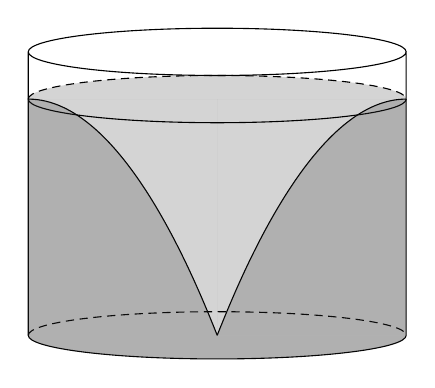
\begin{tikzpicture}[scale=0.6]
      \fill[left color=gray!50!black,right color=gray!50!black,middle color=gray!50!black,shading=axis,opacity=0.10] (0,0) parabola[bend at end] (-4,5) -- (0,5);
      \fill[left color=gray!50!black,right color=gray!50!black,middle color=gray!50!black,shading=axis,opacity=0.10] (0,0) parabola[bend at end] (4,5) -- (0,5);
      \fill[left color=gray!50!black,right color=gray!50!black,middle color=gray!50!black,shading=axis,opacity=0.10] (4,5) arc (360:180:4cm and -0.5cm);
      \draw (-4,6) -- (-4,0) arc (180:360:4cm and 0.5cm) -- (4,6) ++ (-4,0) circle (4cm and 0.5cm);
      \draw[densely dashed] (-4,0) arc (180:0:4cm and 0.5cm);
      \draw[densely dashed] (-4,5) arc (180:0:4cm and 0.5cm);
      \draw (-4,5) -- (-4,5) arc (180:360:4cm and 0.5cm);
      \draw (0,0) parabola[bend at end] (-4,5);
      \draw (0,0) parabola[bend at end] (4,5);
      \fill[left color=gray!50!black,right color=gray!50!black,middle color=gray!50!black,shading=axis,opacity=0.20] (0,0) parabola[bend at end] (-4,5) -- (-4,0) arc (180:360:4cm and 0.5cm);
      \fill[left color=gray!50!black,right color=gray!50!black,middle color=gray!50!black,shading=axis,opacity=0.20] (0,0) parabola[bend at end] (4,5) -- (4,0);
    \end{tikzpicture}
    \caption{Ideal vortex}
  \end{center}
\end{figure}

\subsubsection{Derivation of Velocity Profile}

The irrotational vortex has zero vorticity $\omega$, so all of the components of $\omega=\underline{\nabla}\times\underline{v}$ must be zero.
From the definition for curl in cylindrical coordinates, these components are the following

\begin{equation*}
  \begin{split}
    \frac{1}{r}\frac{\partial{}v_{z}}{\partial\theta}-\frac{\partial{}v_{\theta}}{\partial{}z}&=0 \\
    \frac{\partial{}v_{r}}{\partial{}z}-\frac{\partial{}v_{z}}{\partial{}r}&=0 \\
    \frac{1}{r}\frac{\partial}{\partial{}r}(v_{\theta}r)-\frac{1}{r}\frac{\partial{}v_{r}}{\partial\theta}&=0
  \end{split}
\end{equation*}

The vortex is azimuthally symmetric, so all the $\theta$ derivatives are zero, that is $\frac{\partial}{\partial\theta}=0$, allowing the equations above to simplify to

\begin{equation*}
  \begin{split}
    \frac{\partial{}v_{\theta}}{\partial{}z}&=0 \\
    \frac{\partial{}v_{r}}{\partial{}z}-\frac{\partial{}v_{z}}{\partial{}r}&=0 \\
    \frac{\partial}{\partial{}r}(v_{\theta}r)&=0
  \end{split}
\end{equation*}

From the fact that the vortex is azimuthally symmetric, no properties are functions of $\theta$.
Furthermore, from the first equation we can see that $v_{\theta}$ is not a function of $z$.
That is

\begin{equation*}
  v_{\theta}=v_{\theta}(r)
\end{equation*}

From the third equation, applying product rule we have

\begin{equation*}
  \begin{split}
    r\frac{\partial{}v_{\theta}}{\partial{}r}+v_{\theta}&=0 \\
    -\int\frac{\partial{}r}{r}&=\int\frac{\partial{}v_{\theta}}{v_{\theta}} \\
    -\ln(r)&=\ln(v_{\theta})+c_{1} \\
    \ln(v_{\theta})&=\ln(c)-\ln(r) \\
    \ln(v_{\theta})&=\ln\left(\frac{c}{r}\right) \\
    v_{\theta}&=\frac{c}{r}
  \end{split}
\end{equation*}

\subsubsection{Derivation of Pressure Distribution}

Now write down Euler's equation in each direction.
The partial derivative with respect to time, also known as the local rate of change, is zero, because at a fixed point in the fluid, the velocity is not changing with time.

\begin{equation*}
  \frac{\partial\underline{v}}{\partial{}t}=0
\end{equation*}
Looking at the next term

\begin{equation*}
  \underline{\nabla}=\frac{\partial}{\partial{}r}\hat{\underline{e}}_{r}+\frac{1}{r}\frac{\partial}{\partial\theta}\hat{\underline{e}}_{\theta}+\frac{\partial}{\partial{}z}\hat{\underline{e}}_{z}
\end{equation*}
Now evaluating $(\underline{v}\cdot\underline{\nabla})\underline{v}$

\begin{equation*}
  \begin{split}
    (\underline{v}\cdot\underline{\nabla})\underline{v}&=
    \left(v_{r}\frac{\partial}{\partial{}r}+
    \frac{1}{r}v_{\theta}\frac{\partial}{\partial\theta}+
    v_{z}\frac{\partial}{\partial{}z}\right)\underline{v} \\
    &=v_{r}\frac{\partial}{\partial{}r}\underline{v}+
    \frac{1}{r}v_{\theta}\frac{\partial}{\partial\theta}\underline{v}+
    v_{z}\frac{\partial}{\partial{}z}\underline{v} \\
    &=v_{r}\frac{\partial}{\partial{}r}(v_{r}\hat{\underline{e}}_{r}+v_{\theta}\;\hat{\underline{e}}_{\theta}+v_{z}\;\hat{\underline{e}}_{z})
    +\frac{1}{r}v_{\theta}\frac{\partial}{\partial\theta}(v_{r}\hat{\underline{e}}_{r}+v_{\theta}\;\hat{\underline{e}}_{\theta}+v_{z}\;\hat{\underline{e}}_{z})
    +v_{z}\frac{\partial}{\partial{}z}(v_{r}\hat{\underline{e}}_{r}+v_{\theta}\;\hat{\underline{e}}_{\theta}+v_{z}\;\hat{\underline{e}}_{z}) \\
  \end{split}
\end{equation*}
Now substitute in that $v_{r}=v_{z}=0$ and get

\begin{equation*}
  \begin{split}
    (\underline{v}\cdot\underline{\nabla})\;\underline{v}
    &=\frac{1}{r}v_{\theta}\frac{\partial}{\partial\theta}(v_{\theta}\hat{\underline{e}}_{\theta}) \\
    &=\frac{1}{r}v_{\theta}\frac{\partial{}v_{\theta}}{\partial\theta}\hat{\underline{e}}_{\theta}+\frac{1}{r}v_{\theta}^{2}\frac{\partial\hat{\underline{e}}_{\theta}}{\partial\theta} \\
    &=0+\frac{1}{r}v_{\theta}^{2}\frac{\partial\hat{\underline{e}}_{\theta}}{\partial\theta} \\
    &=-\frac{v_{\theta}^{2}}{r}\hat{\underline{e}}_{r}
  \end{split}
\end{equation*}
The surface force term

\begin{equation*}
  \underline{\nabla}p=\frac{\partial{}p}{\partial{}r}\hat{\underline{e}}_{r}+\frac{1}{r}\frac{\partial{}p}{\partial\theta}\hat{\underline{e}}_{\theta}+\frac{\partial{}p}{\partial{}z}\hat{\underline{e}}_{z}
\end{equation*}
body force term

\begin{equation*}
  \rho\underline{g}=-\rho{}g_{z}\hat{\underline{e}}_{z}
\end{equation*}
Forming the whole equation we have

\begin{equation*}
  -\rho\frac{v_{\theta}^{2}}{r}\hat{\underline{e}}_{r}=-\frac{\partial{}p}{\partial{}r}\hat{\underline{e}}_{r}-\frac{1}{r}\frac{\partial{}p}{\partial\theta}\hat{\underline{e}}_{\theta}-\frac{\partial{}p}{\partial{}z}\hat{\underline{e}}_{z}-\rho{}g_{z}\hat{\underline{e}}_{z}
\end{equation*}
Equating the components we have

\begin{equation*}
  -\rho\frac{v_{\theta}^{2}}{r}=-\frac{\partial{}p}{\partial{}r}
  \hspace{0.5in}
  0=-\frac{1}{r}\frac{\partial{}p}{\partial\theta}
  \hspace{0.5in}
  0=-\frac{\partial{}p}{\partial{}z}-\rho{}g_{z}
\end{equation*}
This gives

\begin{equation*}
  \frac{\partial{}p}{\partial{}r}=\frac{\rho{}c^{2}}{r^{3}}
  \hspace{0.5in}
  \frac{\partial{}p}{\partial\theta}=0
  \hspace{0.5in}
  \frac{\partial{}p}{\partial{}z}=-\rho{}g_{z}
\end{equation*}
separating and integrating these back

\begin{equation*}
  \int\partial{}p=\int\frac{\rho{}c^{2}}{r^{3}}\partial{}r
  \hspace{0.5in}
  \frac{\partial{}p}{\partial\theta}=0
  \hspace{0.5in}
  \int\partial{}p=-\int\rho{}g_{z}\partial{}z
\end{equation*}
The second equation shows that the pressure is not a function of $\theta$.
Integrating back the first and third equations we have the following

\begin{equation*}
  \begin{split}
    p&=-\frac{\rho{}c^{2}}{2r^{2}}+f(z)+k \\
    p&=-\rho{}g_{z}z+g(r)+k
  \end{split}
\end{equation*}
and we have

\begin{equation*}
  \begin{split}
    f(z)&=-\rho{}g_{z}z \\
    g(r)&=-\frac{\rho{}c^{2}}{2r^{2}}
  \end{split}
\end{equation*}
and so the pressure in the rotating cylinder is given by

\begin{equation*}
  p(r,z)=-\frac{\rho{}c^{2}}{2r^{2}}-\rho{}g_{z}z+k
\end{equation*}

From this equation for the pressure in the vortex, we can see that when pressure is a constant, i.e.\ on an isobar, that $z\approx-\frac{1}{r^{2}}$.
We can solve for the constant of integration $c$ by saying when $r=R$, the radius of the tank, $p_{\text{atm}}$ is achieved at a height $h_{0}$.
Plugging this in
\begin{equation*}
  p_{\text{atm}}=-\frac{\rho{}c^{2}}{2R^{2}}-\rho{}g_{z}h_{0}+k
\end{equation*}

\begin{equation*}
  k=p_{\text{atm}}+\frac{\rho{}c^{2}}{2R^{2}}+\rho{}g_{z}h_{0}
\end{equation*}
The final equation is

\begin{empheq}[box=\fboxTwo]{alignat*=3}
  &\mbox{\textbf{Pressure in ideal vortex:}} &\hspace{0.5in} p(r,z)=\frac{\rho{}c^{2}}{2}\left(\frac{1}{R^{2}}-\frac{1}{r^{2}}\right)+p_{\text{atm}}+\rho{}g_{z}(h_{0}-z)
\end{empheq}
To determine the shape that the air-water interface makes, we apply the boundary condition at this interface.
That is

\begin{equation*}
  p(r,z)\bigr|_{\text{interface}}=p_{\text{atm}}
\end{equation*}
And then we have

\begin{equation*}
  0=\frac{\rho{}c^{2}}{2}\left(\frac{1}{R^{2}}-\frac{1}{r_{\text{interface}}^{2}}\right)+\rho{}g_{z}(h_{0}-z_{\text{interface}})
\end{equation*}

\begin{equation*}
  z_{\text{interface}}=\frac{c^{2}}{2g_{z}}\left(\frac{1}{R^{2}}-\frac{1}{r_{\text{interface}}^{2}}\right)+h_{0}
\end{equation*}

\subsubsection{Isobars}

Can also find out the shape of the fluid by solving for isobars by evaluating $dp$ and setting it equal to zero.
Since $p=p(r,z)$ chain rule gives us the following for $dp$.

\begin{equation*}
  dp=\left(\frac{\partial{}p}{\partial{}r}\right)dr+\left(\frac{\partial{}p}{\partial{}z}\right)dz
\end{equation*}

\begin{equation*}
  dp=\frac{\rho{}c_{2}^{2}}{r^{3}}dr-\rho{}g_{z}dz=0
\end{equation*}

\begin{equation*}
  dz=\frac{c_{2}^{2}}{g_{z}r^{3}}dr
\end{equation*}

Integrating back and solving for the constant of integration when $r=0$ we have

\begin{equation*}
  z_{2}-z_{1}=-\frac{c_{2}^{2}}{2g_{z}}\left(\frac{1}{r_{2}^{2}}-\frac{1}{r_{1}^{2}}\right)
\end{equation*}

\begin{equation*}
  z=-\frac{c_{2}^{2}}{2g_{z}}\left(\frac{1}{r^{2}}-\frac{1}{R^{2}}\right)+h_{0}
\end{equation*}

\begin{equation*}
  z=\frac{c_{2}^{2}}{2g_{z}}\left(\frac{1}{R^{2}}-\frac{1}{r^{2}}\right)+h_{0}
\end{equation*}

% TODO@dpwiese
Pretty sure this $c_{2}$ is just supposed to be $c$.

\subsubsection{Problem 10.11}

Has thin inlet in the outer edge of tank to supply water for vortex.
From original equation where we solve for $v_{\theta}$

\begin{equation*}
  c=VR
\end{equation*}

\begin{equation*}
  z=\frac{(VR)^{2}}{2g_{z}}\left(\frac{1}{R^{2}}-\frac{1}{r^{2}}\right)+h_{0}
\end{equation*}

\section{Hydrostatics}

Hydrostatics comes from simplifying Euler's equation by making the acceleration of the fluid element zero, that is $\underline{a}=0$, giving the following equation

\begin{equation*}
  -\underline{\nabla}p+\rho\underline{g}=0
\end{equation*}

\chapter{Gauss' and Stokes' Theorem}

\section{Gauss' Theorem}

% TODO@dpwiese - does this equation need an extra `+p_{\text{atm}}` term on RHS?
\begin{empheq}[box=\fboxTwo]{alignat*=3}
  &\mbox{\textbf{Gauss' Theorem:}} \hspace{0.5in} & \int_{V}(\underline{\nabla}\cdot\underline{v})dV=\oint_{S}\underline{v}\cdot\underline{dA}
\end{empheq}

\section{Stokes' Theorem}

\begin{empheq}[box=\fboxTwo]{alignat*=3}
  &\mbox{\textbf{Stokes' Theorem:}} \hspace{0.5in} & \int_{A}\underbrace{(\underline{\nabla}\times\underline{v})}_{\text{vorticity}}\cdot dA=\underbrace{\oint_{C}\underline{v}\cdot\underline{dl}}_{\text{circulation}}
\end{empheq}

And $\Gamma$ is called the circulation.
Stokes' theorem relates the area integral of vorticity to circulation.

\begin{equation*}
  \Gamma=\oint_{C}\underline{v}\cdot\underline{dl}
\end{equation*}

\chapter{Control Surfaces, Volumes, and Masses}

\section{More on Conservation Equations: Forms A and B}

\begin{empheq}[box={\labelBox[Mass Conservation]}]{alignat*=3}
  &\mbox{\textbf{Form A:}} &\hspace{0.5in} \frac{d}{dt}\int_{CV(t)}\rho{}dV+\int_{CS(t)}\rho{}(\overline{v}-\overline{v}_{c})\cdot\overline{n}dA=0 \\[6pt]
  &\mbox{\textbf{Form B:}} &\hspace{0.5in} \int_{CV(t)}\frac{\partial\rho}{\partial{}t}dV+\int_{CS(t)}\rho{}v_{n}dA=0
\end{empheq}

\begin{equation*}
  v_{rn}=(\overline{v}-\overline{v}_{c})\cdot\overline{n}
\end{equation*}

$\overline{v}$ is the velocity across the control surface.

\begin{empheq}[box={\labelBox[Momentum Conservation]}]{alignat*=3}
  &\mbox{\textbf{Form A:}} &\hspace{0.5in} \frac{d}{dt}\int_{CV(t)}\rho\overline{v}dV+\int_{CS(t)}\rho\overline{v}(\overline{v}-\overline{v}_{c})\cdot\overline{n}dA=\overline{F}_{CV}(t) \\[6pt]
  &\mbox{\textbf{Form B:}} &\hspace{0.5in} \int_{CV(t)}\frac{\partial(\rho\overline{v})}{\partial{}t}dV+\int_{CS(t)}\rho\overline{v}v_{n}dA=\overline{F}_{CV}(t)
\end{empheq}

\chapter{Viscous Flow}

The Newtonian stress tensor $\uuline{\tau}$ contains contributions of normal stress from pressure, as well as shear stresses in the form of the viscous stress tensor $\uuline{\sigma}$.
Thus, the Newtonian stress tensor can be written as the following, where for an inviscid fluid $\uuline{\sigma}=0$.
The viscous stress tensor is a tensor used in continuum mechanics to model the part of the stress at a point within some material that can be attributed to the strain rate, the rate at which it is deforming around that point.

\begin{empheq}[box=\fboxTwo]{alignat*=3}
  &\mbox{\textbf{Inviscid}} \hspace{0.5in} & \uuline{\tau}=-p\uuline{I} \\
  &\mbox{\textbf{Viscous}} \hspace{0.5in} & \uuline{\tau}=-p\uuline{I}+\uuline{\sigma}
\end{empheq}

\begin{defn-dan}[Newton's viscosity law (Viscosity)]
  \begin{empheq}[box=\roomyfbox]{equation*}
    \text{viscosity}=-\frac{\text{shear stress}}{\text{rate of shear deformation or strain}}
  \end{empheq}

  \begin{equation*}
    \mu=-\frac{\tau}{\frac{d\gamma}{dt}}
  \end{equation*}
\end{defn-dan}

This is what it is to be a Newtonian fluid, one where the shear stress is proportional to the shear strain rate, where the constant of proportionality is called the fluid's viscosity.

\begin{defn-dan}[Reynolds number]
  The Reynolds number is the ratio between the inertial viscous forces in a fluid.
  \begin{equation*}
    \text{Re}=\frac{\rho{}Ul}{\mu}
  \end{equation*}
\end{defn-dan}

Airplanes flying at high altitude (rarefied gas) the density is very low, which means the Reynolds number is very small.
This is the same effect as highly viscous flow.
Basically $\underline{\nabla}\;\underline{v}$ is the divergence of the velocity field.
Thinking about this in terms of a square fluid element in some velocity field, $\underline{\nabla}\;\underline{v}$ describes how this fluid element will move with time.
This movement can cause the fluid element to translate, rotate, and deform.
We would like to split these three parts up.

\begin{equation*}
  \begin{split}
    \underline{\nabla}\;\underline{u}&=\frac{1}{2}\left(\underline{\nabla}\;\underline{u}+(\underline{\nabla}\;\underline{u})^{\top}\right)+\frac{1}{2}\left(\underline{\nabla}\;\underline{u}-(\underline{\nabla}\;\underline{u})^{\top}\right) \\
    &=\uuline{e}+\uuline{\Omega}
  \end{split}
\end{equation*}

\begin{empheq}[box=\fboxTwo]{alignat*=3}
  &\mbox{\textbf{Strain rate tensor:}} &\hspace{0.5in} \uuline{e}=\frac{1}{2}\left(\underline{\nabla}\;\underline{u}+(\underline{\nabla}\;\underline{u})^{\top}\right) \\
  &\mbox{\textbf{Rotation rate tensor:}} &\hspace{0.5in} \uuline{\Omega}=\frac{1}{2}\left(\underline{\nabla}\;\underline{u}-(\underline{\nabla}\;\underline{u})^{\top}\right)
\end{empheq}

Can derive from pictures

\begin{equation*}
  \uuline{\sigma}=2\mu\uuline{e}
\end{equation*}

For incompressible flows with constant viscosity

\begin{equation*}
  \underline{\nabla}\cdot\underline{v}=0
\end{equation*}

The strain rate tensor represents shearing/stretching of the fluid element.

% Define dimensions for rotation of fluid element diagram
\newdimen\myx{}
\newdimen\myy{}

\begin{figure}[H]
  \centering
  \begin{minipage}[b]{0.22\linewidth}
    \begin{center}
      \begin{tikzpicture}[scale=1.1, media/.style={font={\footnotesize\sffamily}}, interface/.style={postaction={draw,decorate,decoration={border,angle=-45, amplitude=0.3cm,segment length=2mm}}}]
        \draw[dashed] (0,0) -- (0,2);
        \draw[dashed] (0,0) -- (2,0);
        \draw[dashed] (0,2) -- (2,2);
        \draw[dashed] (2,0) -- (2,2);
        \draw (1,0.5) -- (1,2.5);
        \draw (1,0.5) -- (3,0.5);
        \draw (1,2.5) -- (3,2.5);
        \draw (3,0.5) -- (3,2.5);
      \end{tikzpicture}
      % \caption{Translation}
    \end{center}
  \end{minipage}
  \quad
  \begin{minipage}[b]{0.22\linewidth}
    \begin{center}
      \begin{tikzpicture}[ scale=1.1, media/.style={font={\footnotesize\sffamily}}, interface/.style={postaction={draw,decorate,decoration={border,angle=-45, amplitude=0.3cm,segment length=2mm}}}]
        \draw[dashed] (0,0) -- (0,2);
        \draw[dashed] (0,0) -- (2,0);
        \draw[dashed] (0,2) -- (2,2);
        \draw[dashed] (2,0) -- (2,2);
        \coordinate (x) at (1, 1);
        \pgfextractx{\myx}{\pgfpointanchor{x}{center}}
        \pgfextracty{\myy}{\pgfpointanchor{x}{center}}
        \pgftransformshift{\pgfqpoint{\myx}{\myy}}
        \pgftransformrotate{20}
        \pgftransformshift{\pgfqpoint{-\myx}{-\myy}}
        \draw (0,0) -- (0,2);
        \draw (0,0) -- (2,0);
        \draw (0,2) -- (2,2);
        \draw (2,0) -- (2,2);
      \end{tikzpicture}
      % \caption{Rotation}
    \end{center}
  \end{minipage}
  \quad
  \begin{minipage}[b]{0.22\linewidth}
    \begin{center}
      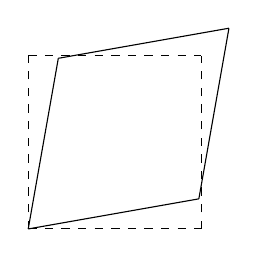
\begin{tikzpicture}[ scale=1.1, media/.style={font={\footnotesize\sffamily}}, interface/.style={postaction={draw,decorate,decoration={border,angle=-45, amplitude=0.3cm,segment length=2mm}}}]
        \draw[dashed] (0,0) -- (0,2);
        \draw[dashed] (0,0) -- (2,0);
        \draw[dashed] (0,2) -- (2,2);
        \draw[dashed] (2,0) -- (2,2);
        \draw[rotate=-10] (0,0) -- (0,2) node[name=A]{};
        \draw[rotate=10] (0,0) -- (2,0) node[name=B]{};
        \draw[rotate=-80] (A.center) --++ (0,2);
        \draw[rotate=80] (B.center) --++ (2,0);
      \end{tikzpicture}
      % \caption{Shearing}
    \end{center}
  \end{minipage}
  \quad
  \begin{minipage}[b]{0.22\linewidth}
    \begin{center}
      \begin{tikzpicture}[ scale=1.1, media/.style={font={\footnotesize\sffamily}}, interface/.style={postaction={draw,decorate,decoration={border,angle=-45, amplitude=0.3cm,segment length=2mm}}}]
      \draw[dashed] (0,0) -- (0,2);
      \draw[dashed] (0,0) -- (2,0);
      \draw[dashed] (0,2) -- (2,2);
      \draw[dashed] (2,0) -- (2,2);
      \draw (0.2,0.2) -- (0.2,1.8);
      \draw (0.2,0.2) -- (1.8,0.2);
      \draw (1.8,0.2) -- (1.8,1.8);
      \draw (0.2,1.8) -- (1.8,1.8);
      \end{tikzpicture}
      % \caption{Pure compression}
    \end{center}
  \end{minipage}
  \caption{a.\ Translation, b.\ rotation, c.\ shearing, d.\ Pure compression}
\end{figure}

\section{Derivation of Incompressible Navier-Stokes' Equations}

The Navier Stokes' Equation describes conservation of linear momentum for isothermal flow of an incompressible newtonian fluid.

\begin{figure}[H]
  \begin{center}
    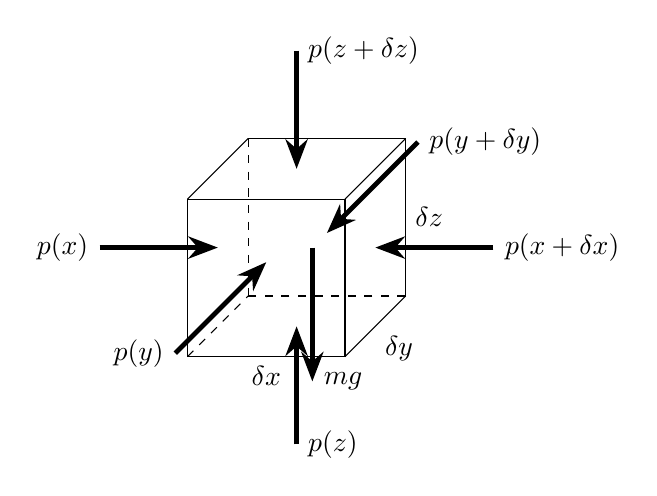
\begin{tikzpicture}[>=Stealth]
      \def\sliceZ{0.8}
      \def\side{2}
      \def\linewidth{0.6}
      \def\arrowlength{1.5}
      \draw[dashed] (\side,0,0) -- (0,0,0);
      \draw[dashed] (0,0,\side) -- (0,0,0);
      \draw[dashed] (0,\side,0) -- (0,0,0);
      \draw (\side,0,0) -- (\side,\side,0) node[midway,right]{$\delta z$} -- (0,\side,0);
      \draw (0,0,\side) -- (\side,0,\side) node[midway,below]{$\delta x$} -- (\side,\side,\side) -- (0,\side,\side) -- (0,0,\side);
      \draw (\side,0,0) -- (\side,0,\side) node[midway,below right]{$\delta y$};
      \draw (\side,\side,0) -- (\side,\side,\side);
      \draw (0,\side,0) -- (0,\side,\side);
      \node at (1,\sliceZ,1){};
      \draw[line width=\linewidth mm,->](\side+\arrowlength,\side/2,\side/2) node[right]{$p(x+\delta x)$} -- (\side,\side/2,\side/2);
      \draw[line width=\linewidth mm,->](-\arrowlength,\side/2,\side/2) node[left]{$p(x)$} -- (0,\side/2,\side/2);
      \draw[line width=\linewidth mm,->](\side/2,\side/2+0.2,\side+3) node[left]{$p(y)$} -- (\side/2,\side/2+0.2,\side);
      \draw[line width=\linewidth mm,->](\side/2,\side/2-0.2,-3) node[right]{$p(y+\delta y)$} -- (\side/2,\side/2-0.2,0);
      \draw[line width=\linewidth mm,->](\side/2,\side+\arrowlength,\side/2) node[right]{$p(z+\delta z)$} -- (\side/2,\side,\side/2);
      \draw[line width=\linewidth mm,->](\side/2,-\arrowlength,\side/2) node[right]{$p(z)$} -- (\side/2,0,\side/2);
      \draw[line width=\linewidth mm,->](\side/2+0.2,\side/2,\side/2) -- (\side/2+0.2,\side/2-\arrowlength-0.2,\side/2) node[right]{$mg$};
    \end{tikzpicture}
    \caption{Fluid element with pressure and gravity acting on it}
  \end{center}
\end{figure}

Summing the forces in the $x$, $y$, and $z$ directions we have

\begin{equation*}
  \begin{split}
    p\delta y\delta z-\left(p+\frac{\partial{}p}{\partial{}x}\right)\delta y\delta z&=\rho\delta x\delta y\delta za_{x} \\
    p\delta x\delta z-\left(p+\frac{\partial{}p}{\partial{}y}\right)\delta x\delta z&=\rho\delta x\delta y\delta za_{y} \\
    p\delta x\delta y-\left(p+\frac{\partial{}p}{\partial{}z}\right)\delta x\delta y-\rho{}g_{z}\delta x\delta y\delta z&=\rho\delta x\delta y\delta za_{z} \\
  \end{split}
\end{equation*}

% TODO@dpwiese - finish the below?
simplifying

\begin{empheq}[box=\fboxTwo]{alignat*=3}
  &\mbox{\textbf{Incompressible Navier-Stokes}} \hspace{0.5in}& \rho\left(\frac{\partial\underline{v}}{\partial{}t}+\underline{v}\cdot\underline{\nabla}\underline{v}\right)=-\underline{\nabla}p+\mu\nabla^{2}\underline{v}+\rho\underline{g} \\
  & &\hspace{0.5in} \rho\frac{D\underline{v}}{Dt}=-\underline{\nabla}p+\underline{\nabla}\cdot\uuline{\sigma}+\rho\underline{g} \\
  & &\hspace{0.5in} \rho\frac{D\underline{v}}{Dt}=-\underline{\nabla}p+\mu\nabla^{2}\underline{v}+\rho\underline{g}
\end{empheq}

Fully developed flow implies that the velocity profile does not change in the fluid flow direction hence the momentum also does not change in the flow direction.
In such a case, the pressure in the flow direction will balance the shear stress near the wall.

The assumptions of the equation are that the fluid is incompressible and newtonian; the flow is laminar through a pipe of constant circular cross-section that is substantially longer than its diameter; and there is no acceleration of fluid in the pipe.
For velocities and pipe diameters above a threshold, actual fluid flow is not laminar but turbulent, leading to larger pressure drops than calculated by the Hagen$-$Poiseuille equation.

\section{Exact Solutions to the Navier-Stokes Equations}

Some cases where an exact analytic solution to the Navier-Stokes equations exist are for the steady case Poisseiulle flow (viscous flow through a circular pipe, or between two long parallel plates) and Coutte flow (laminar flow between two parallel plates where one is moving).
In other time dependent cases we have Stokes' first and second problems.

\subsection{Poiseuille Flow in Circular Pipe}

In this section we derive of Poiseuille flow in a circular pipe from Navier-Stokes equation.
The laminar flow through a pipe of uniform (circular) cross-section is one of two cases known as Hagen$-$Poiseuille flow.
In this case, we make the following assumptions:

\begin{empheq}[box={\labelBox[Circular Pipe Poiseuille Flow]}]{alignat*=3}
  &\mbox{\textbf{Steady:}} &\hspace{0.5in} \frac{\partial}{\partial{}t}=0 \\
  &\mbox{\textbf{No radial or swirl velocity:}} &\hspace{0.5in} v_{r}=v_{\theta}=0 \\
  &\mbox{\textbf{Radially symmetric:}} &\hspace{0.5in} \frac{\partial}{\partial\theta}=0 \\
  &\mbox{\textbf{Fully developed:}} &\hspace{0.5in} \frac{\partial{}v_{z}}{\partial{}z}=0 \\
  &\mbox{\textbf{Gravity is neglible:}} &\hspace{0.5in} \underline{g}=0
\end{empheq}

In a large pipe we can have hydrostatic pressure variations, but usually these are very small and can be neglected.
\textit{Use the Navier-Stokes' equation sheet to obtain the expanded equations in cylindrical coordinates.}
Simplifying the Navier-Stokes equations using the above assumptions we have

\begin{equation*}
  \begin{split}
    0&=-\frac{\partial{}p}{\partial{}r} \\
    0&=-\frac{\partial{}p}{\partial\theta} \\
    0&=\mu\left[\frac{1}{r}\frac{\partial}{\partial{}r}\left(r\frac{\partial{}v_{z}}{\partial{}r}\right)\right]-\frac{\partial{}p}{\partial{}z}
  \end{split}
\end{equation*}

The first two equations show that the pressure in the tube is only a function of $z$.
Because of this, the partial derivative in the third equation can be made a full derivative, and then we can integrate this equation back to find the an expression for the velocity along the pipe, $v_{z}$.

\begin{equation*}
  \begin{split}
    0&=\mu\left[\frac{1}{r}\frac{\partial}{\partial{}r}\left(r\frac{\partial{}v_{z}}{\partial{}r}\right)\right]-\frac{dp}{dz} \\
    \frac{dp}{dz}&=\frac{\mu}{r}\frac{\partial}{\partial{}r}\left(r\frac{\partial{}v_{z}}{\partial{}r}\right) \\
    \int\frac{dp}{dz}r\partial{}r&=\int\mu\partial\left(r\frac{\partial{}v_{z}}{\partial{}r}\right) \\
    \frac{1}{2}\frac{dp}{dz}r^{2}+c_{3}&=\mu{}r\frac{\partial{}v_{z}}{\partial{}r} \\
    \frac{1}{2}\frac{dp}{dz}r+\frac{c_{3}}{r}&=\mu\frac{\partial{}v_{z}}{\partial{}r} \\
    \int\left(\frac{1}{2}\frac{dp}{dz}r+\frac{c_{3}}{r}\right)\partial{}r&=\int\mu\partial{}v_{z} \\
    \frac{1}{4}\frac{dp}{dz}r^{2}+c_{3}\ln{r}+c_{4}&=\mu{}v_{z} \\
    v_{z}&=\frac{1}{4\mu}\frac{dp}{dz}r^{2}+c_{1}\ln{r}+c_{2}
  \end{split}
\end{equation*}

\begin{empheq}[box=\roomyfbox]{equation*}
  v_{z}=\frac{1}{4\mu}\frac{dp}{dz}r^{2}+c_{1}\ln{r}+c_{2}
\end{empheq}

\subsubsection{Applying Boundary Conditions}

Here we need to use the boundary conditions to find the constants $c_{1}$ and $c_{2}$.

\subsubsection{Regular Pipe}

\begin{figure}[H]
  \begin{center}
    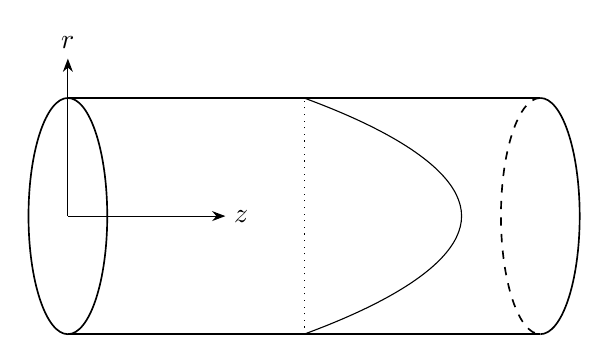
\begin{tikzpicture}[>=Stealth,scale=1.0]
      \draw[semithick]  (0.5,0) arc (360:0:0.5 and 1.5);
      \draw[semithick]  (6,1.5) arc (90:-90:0.5 and 1.5);
      \draw[semithick, dashed,color=black] (6,1.5) arc (90:270:0.5 and 1.5);
      \draw[semithick] (0,-1.5) -- (6,-1.5);
      \draw[semithick] (0,1.5) -- (6,1.5);
      \draw[->](0,0) -- (2,0) node[pos=1.1]{$z$};
      \draw[->](0,0) -- (0,2) node[pos=1.1]{$r$};
      \draw[rotate=-90] (1.5,3) parabola[bend at end] (0,5);
      \draw[rotate=-90] (-1.5,3) parabola[bend at end] (0,5);
      \draw[dotted] (3,-1.5) -- (3,1.5);
    \end{tikzpicture}
    \caption{Parabolic velocity profile for Poiseuille flow through a circular pipe}
  \end{center}
\end{figure}

\begin{empheq}[box=\fboxTwo]{alignat*=3}
  &\mbox{\textbf{Finite velocity along center of pipe:}} &\hspace{0.5in} v_{z}(r=0)=\text{finite} \\
  &\mbox{\textbf{No slip at pipe wall:}} &\hspace{0.5in} v_{z}(R)=0
\end{empheq}

From the first boundary condition, when $r=0$, $v_{z}$ must be finite.
Looking at $c_{1}\ln{r}$ when $r=0$ we see that this term goes to infinity when $r$ goes to zero.
To prevent the velocity from going to infinity $c_{1}$ must be zero.
Now look at the second boundary condition

\begin{equation*}
  \begin{split}
    0&=\frac{1}{4\mu}\frac{dp}{dz}R^{2}+c_{2} \\
    c_{2}&=-\frac{1}{4\mu}\frac{dp}{dz}R^{2}
  \end{split}
\end{equation*}

so we have

\begin{equation*}
  v_{z}=\frac{1}{4\mu}\frac{dp}{dz}r^{2}-\frac{1}{4\mu}\frac{dp}{dz}R^{2}
\end{equation*}

\begin{empheq}[box=\fboxTwo]{alignat*=3}
  &\mbox{\textbf{Velocity for Poiseuille flow in regular pipe:}} &\hspace{0.5in} v_{z}&=-\frac{1}{4\mu}\frac{dp}{dz}(R^{2}-r^{2})
\end{empheq}

Now we can integrate the velocity across the pipe to get the average velocity and flow rate.
Furthermore, we can see that the velocity decreases away from the center of the pipe, where the velocity is maximum.
The maximum velocity is

\begin{empheq}[box=\fboxTwo]{alignat*=3}
  &\mbox{\textbf{Maximum velocity for Poiseuille flow in regular pipe:}} &\hspace{0.5in} v_{z,\text{max}}&=-\frac{R^{2}}{4\mu}\frac{dp}{dz}
\end{empheq}

Integrating to find the average velocity and flow rate, which are related by $Q=v_{z,\text{max}}A$ we have the following, where $dA=2\pi{}rdr$.

\begin{equation*}
  Q=\int_{A}-\frac{1}{4\mu}\frac{dp}{dz}(R^{2}-r^{2})dA
\end{equation*}

\begin{equation*}
  Q=-\frac{\pi}{2\mu}\frac{dp}{dz}\int_{0}^{R}(R^{2}-r^{2})rdr
\end{equation*}

\begin{equation*}
  Q=-\frac{\pi}{4\mu}\frac{dp}{dz}\left[\frac{1}{2}R^{2}r^{2}-\frac{1}{4}r^{4}\right]_{0}^{R}
\end{equation*}

\begin{empheq}[box=\fboxTwo]{alignat*=3}
  &\mbox{\textbf{Volume flow rate for Poiseuille flow in regular pipe:}} &\hspace{0.5in} Q&=-\frac{\pi}{8\mu}\frac{dp}{dz}R^{4}
\end{empheq}

The average velocity is then given by

\begin{equation*}
  v_{z,\text{avg}}=\frac{Q}{A}
\end{equation*}

\begin{empheq}[box=\fboxTwo]{alignat*=3}
  &\mbox{\textbf{Average velocity for Poiseuille flow in regular pipe:}} &\hspace{0.5in} v_{z,\text{avg}}&=-\frac{1}{8\mu}\frac{dp}{dz}R^{2}
\end{empheq}

Conservation of mass, and the fully developed assumption gave the condition that the velocity distribution along the pipe is constant.
Once the Navier Stokes' equations are solved, the equation for velocity distribution is expressed in terms of the pressure gradient down the pipe.
Since we know for any given value of $r$ that the velocity is constant along the $z$ direction, we can see that the pressure gradient is constant.
This allows us to replace the pressure gradient in all of the above equations with the pressure drop along a length of pipe

\begin{equation*}
  -\frac{dp}{dz}=\frac{\Delta{}p}{L}
\end{equation*}

In particular, we can use this expression with the flow rate equation, and solve for the pressure drop as a function of pipe length, flow rate, and diameter, among others.
From this we can see that to minimize pressure drop we want a pipe with a large diameter.

\begin{empheq}[box={\labelBox[Pipe Poiseuille Flow]}]{alignat*=3}
  &\mbox{\textbf{Velocity}} \hspace{0.5in}& v_{z}&=\frac{1}{4\mu}\frac{\Delta{}p}{L}(R^{2}-r^{2}) \\
  &\mbox{\textbf{Maximum velocity}} &\hspace{0.5in} v_{z,\text{max}}&=\frac{R^{2}}{4\mu}\frac{\Delta{}p}{L} \\
  &\mbox{\textbf{Average velocity}} &\hspace{0.5in} v_{z,\text{avg}}&=\frac{1}{8\mu}\frac{\Delta{}p}{L}R^{2} \\
  &\mbox{\textbf{Flow rate}} &\hspace{0.5in} Q&=\frac{\pi}{8\mu}\frac{\Delta{}p}{L}R^{4} \\
  &\mbox{\textbf{Pressure drop}} &\hspace{0.5in} \Delta{}p&=\frac{128\mu{}LQ}{\pi{}D^{4}}
\end{empheq}

\subsubsection{Annulus Pipe}

This problem is from 6.04 of Shapiro and Sonin problems.

\begin{figure}[H]
  \begin{center}
    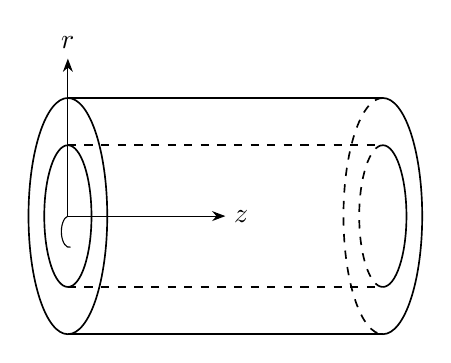
\begin{tikzpicture}[>=Stealth,scale=1.0]
      \draw[semithick]  (0.5,0) arc (360:0:0.5 and 1.5);
      \draw[semithick]  (4,1.5) arc (90:-90:0.5 and 1.5);
      \draw[semithick, dashed,color=black] (4,1.5) arc (90:270:0.5 and 1.5);
      \draw[semithick] (0,-1.5) -- (4,-1.5);
      \draw[semithick] (0,1.5) -- (4,1.5);
      \draw[semithick]  (0.3,0) arc (360:0:0.3 and 0.9);
      \draw[semithick]  (4,0.9) arc (90:-90:0.3 and 0.9);
      \draw[semithick, dashed,color=black] (4,0.9) arc (90:270:0.3 and 0.9);
      \draw[semithick, dashed] (0,-0.9) -- (4,-0.9);
      \draw[semithick, dashed] (0,0.9) -- (4,0.9);
      \draw[->](0,0) -- (2,0) node[pos=1.1]{$z$};
      \draw[->](0,0) -- (0,2) node[pos=1.1]{$r$};
      \draw (0,0) arc (100:280:0.1 and 0.2);
    \end{tikzpicture}
  \end{center}
\end{figure}

\begin{empheq}[]{alignat*=3}
  &\mbox{\textbf{No slip at pipe wall:}} &\hspace{0.5in} v_{z}(R_{1})=0 \\
  &\mbox{\textbf{No slip at pipe wall:}} &\hspace{0.5in} v_{z}(R_{2})=0
\end{empheq}

\begin{equation*}
  \begin{split}
    0&=\frac{1}{4\mu}\frac{dp}{dz}R_{1}^{2}+c_{1}\ln{R_{1}}+c_{2} \\
    0&=\frac{1}{4\mu}\frac{dp}{dz}R_{2}^{2}+c_{1}\ln{R_{2}}+c_{2}
  \end{split}
\end{equation*}

Let $A=\frac{1}{4\mu}\frac{dp}{dz}$

\begin{equation*}
  \begin{split}
    0&=AR_{1}^{2}+c_{1}\ln{R_{1}}+c_{2} \\
    0&=AR_{2}^{2}+c_{1}\ln{R_{2}}+c_{2}
  \end{split}
\end{equation*}

\begin{equation*}
  \begin{split}
    AR_{1}^{2}+c_{1}\ln{R_{1}}&=AR_{2}^{2}+c_{1}\ln{R_{2}} \\
    A(R_{1}^{2}-R_{2}^{2})&=c_{1}(\ln{R_{2}}-\ln{R_{1}}) \\
    c_{1}&=\frac{A(R_{1}^{2}-R_{2}^{2})}{\ln\left(\frac{R_{2}}{R_{1}}\right)} \\
    c_{1}&=\frac{\frac{1}{4\mu}\frac{dp}{dz}(R_{1}^{2}-R_{2}^{2})}{\ln\left(\frac{R_{2}}{R_{1}}\right)}
  \end{split}
\end{equation*}

\begin{equation*}
  \begin{split}
    c_{2}&=-\frac{1}{4\mu}\frac{dp}{dz}R_{2}^{2}-c_{1}\ln{R_{2}} \\
    c_{2}&=-\frac{1}{4\mu}\frac{dp}{dz}R_{2}^{2}-\frac{\frac{1}{4\mu}\frac{dp}{dz}(R_{1}^{2}-R_{2}^{2})}{\ln\left(\frac{R_{2}}{R_{1}}\right)}\ln{R_{2}} \\
    c_{2}&=-\frac{1}{4\mu}\frac{dp}{dz}\left(R_{2}^{2}+\frac{(R_{1}^{2}-R_{2}^{2})\ln{R_{2}}}{\ln\left(\frac{R_{2}}{R_{1}}\right)}\right)
  \end{split}
\end{equation*}

\begin{equation*}
  v_{z}=\frac{1}{4\mu}\frac{dp}{dz}r^{2}+c_{1}\ln{r}+c_{2}
\end{equation*}

\begin{empheq}[box=\roomyfbox]{equation*}
  v_{z}=\frac{1}{4\mu}\frac{dp}{dz}r^{2}+\left[\frac{\frac{1}{4\mu}\frac{dp}{dz}(R_{1}^{2}-R_{2}^{2})}{\ln\left(\frac{R_{2}}{R_{1}}\right)}\right]\ln{r}+\left[-\frac{1}{4\mu}\frac{dp}{dz}\left(R_{2}^{2}+\frac{(R_{1}^{2}-R_{2}^{2})\ln{R_{2}}}{\ln\left(\frac{R_{2}}{R_{1}}\right)}\right)\right]
\end{empheq}

\subsection{Derivation of Plane Poiseuille Flow from Navier-Stokes}

Consider the following parallel plates

\begin{figure}[H]
  \begin{center}
    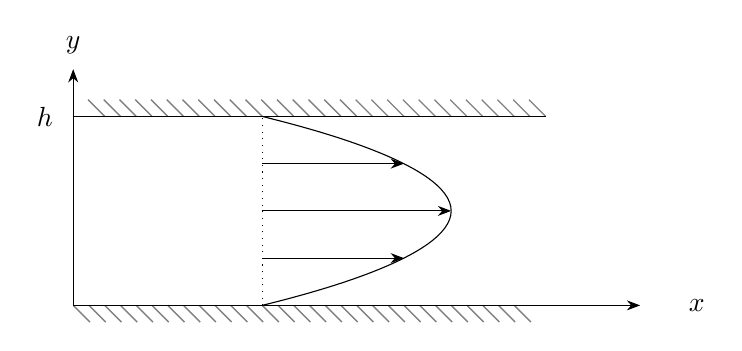
\begin{tikzpicture}[>=Stealth,scale=1.2, media/.style={font={\footnotesize\sffamily}}, interface/.style={postaction={draw,decorate,decoration={border,angle=-45, amplitude=0.3cm,segment length=2mm}}}]
      \draw[->](0,0) -- (6,0) node[pos=1.1]{$x$};
      \draw[->](0,0) -- (0,2.5) node[pos=1.1]{$y$};
      \draw[->](2,0.5) -- (3.5,0.5);
      \draw[->](2,1) -- (4,1);
      \draw[->](2,1.5) -- (3.5,1.5);
      \draw[gray,line width=.5pt,interface](0,0)--(5,0);
      \draw[gray,line width=.5pt,interface](5,2)--(0,2);
      \draw[semithick] (0,2) -- (5,2);
      \draw[semithick] (0,0) -- (5,0);
      \draw (-0.3,2) node {$h$};
      \draw[rotate=-90] (0,2) parabola[bend at end] (-1,4);
      \draw[rotate=-90] (-2,2) parabola[bend at end] (-1,4);
      \draw[dotted] (2,0) -- (2,2);
    \end{tikzpicture}
    \caption{Parabolic velocity profile for plane Poisseiulle flow}
  \end{center}
\end{figure}

\begin{empheq}[]{alignat*=3}
  &\mbox{\textbf{Steady:}} &\hspace{0.5in} \frac{\partial}{\partial{}t}=0 \\
  &\mbox{\textbf{No vertical velocity:}} &\hspace{0.5in} v_{y}=0 \\
  &\mbox{\textbf{2-D flow:}} &\hspace{0.5in} \frac{\partial}{\partial{}z}=0 \\
  & &\hspace{0.5in} v_{z}=0 \\
  &\mbox{\textbf{Fully developed:}} &\hspace{0.5in} \frac{\partial{}v_{x}}{\partial{}x}=0
\end{empheq}

\begin{equation*}
  \begin{split}
    0&=\mu\frac{\partial^{2}v_{x}}{\partial{}y^{2}}-\frac{\partial{}p}{\partial{}x} \\
    0&=-\frac{\partial{}p}{\partial{}y}+\rho{}g_{y} \\
    0&=-\frac{\partial{}p}{\partial{}z}+\rho{}g_{z} \\
  \end{split}
\end{equation*}

Basically need to solve

\begin{equation*}
  0=\mu\frac{\partial^{2}v_{x}}{\partial{}y^{2}}-\frac{\partial{}p}{\partial{}x}
\end{equation*}

\begin{equation*}
  \frac{\partial{}p}{\partial{}x}\partial{}y =\mu\partial\frac{\partial{}v_{x}}{\partial{}y}
\end{equation*}

\begin{equation*}
  \left[\frac{\partial{}p}{\partial{}x}y\right]+C_{1} =\mu\frac{\partial{}v_{x}}{\partial{}y}
\end{equation*}

\begin{equation*}
  \left[\frac{\partial{}p}{\partial{}x}y+C_{1}\right]\partial{}y =\mu\partial{}v_{x}
\end{equation*}

\begin{equation*}
  \frac{1}{2}\frac{\partial{}p}{\partial{}x}y^{2}+C_{1}y+C_{2}=\mu{}v_{x}
\end{equation*}

And using the boundary conditions, we have that $v_{x}(0)=0$ and $v_{x}(h)=0$ so

\begin{equation*}
  C_{2}=0
\end{equation*}

\begin{equation*}
  C_{1}=-\frac{1}{2}\frac{\partial{}p}{\partial{}x}h
\end{equation*}

\begin{empheq}[box=\roomyfbox]{alignat*=3}
  &\mbox{\textbf{Velocity for plane Poisseiulle flow:}} &\hspace{0.5in} v_{x}(y)=-\frac{h^{2}}{2\mu}\frac{\partial{}p}{\partial{}x}\frac{y}{h}\left(1-\frac{y}{h}\right)
\end{empheq}

\subsubsection{Finding volume flow rate}

\subsection{Plane Coutte Flow}

\begin{figure}[H]
  \begin{center}
    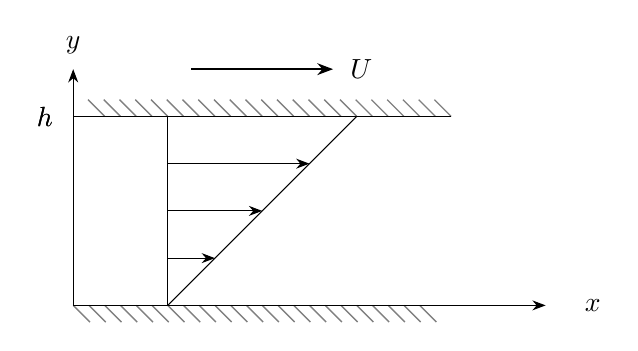
\begin{tikzpicture}[>=Stealth,scale=1.2, media/.style={font={\footnotesize\sffamily}}, interface/.style={postaction={draw,decorate,decoration={border,angle=-45, amplitude=0.3cm,segment length=2mm}}}]
      \draw[->](0,0) -- (5,0) node[pos=1.1]{$x$};
      \draw[->](0,0) -- (0,2.5) node[pos=1.1]{$y$};
      \draw (1,0) -- (1,2);
      \draw (1,0) -- (3,2);
      \draw[->](1,1) -- (2,1);
      \draw[->](1,0.5) -- (1.5,0.5);
      \draw[->](1,1.5) -- (2.5,1.5);
      \draw[semithick, ->](1.25,2.5) -- (2.75,2.5) node[pos=1.2]{$U$};
      \draw (-0.3,2) -- (-0.3,2) node[pos=1.1]{$h$};
      \draw[gray,line width=.5pt,interface](0,0)--(4,0);
      \draw[gray,line width=.5pt,interface](4,2)--(0,2);
      \draw[semithick] (0,2) -- (4,2);
      \draw[semithick] (0,0) -- (4,0);
      \draw (-0.3,2) node {$h$};
    \end{tikzpicture}
    \caption{Linear velocity profile for plane Couette flow}
  \end{center}
\end{figure}

Couette flow is flow driven by moving one plate relative to another.

\begin{empheq}[]{alignat*=3}
  &\mbox{\textbf{Steady:}} &\hspace{0.5in} \frac{\partial}{\partial{}t}=0 \\
  &\mbox{\textbf{Laminar:}} &\hspace{0.5in} v_{y}=v_{z}=0 \\
  &\mbox{\textbf{Symmetric:}} &\hspace{0.5in} \frac{\partial}{\partial{}z}=0 \\
  &\mbox{\textbf{Fully developed:}} &\hspace{0.5in} \frac{\partial{}v_{x}}{\partial{}x}=0
\end{empheq}

\textit{Use the Navier-Stokes' equation sheet to obtain the expanded equations in cartesian coordinates.}
Simplifying the Navier-Stokes equations using the above assumptions we have

\begin{equation*}
  \begin{split}
    0&=\mu\frac{\partial^{2}v_{x}}{\partial{}y^{2}}-\frac{\partial{}p}{\partial{}x} \\
    0&=-\frac{\partial{}p}{\partial{}y}+\rho{}g_{y} \\
    0&=-\frac{\partial{}p}{\partial{}z}+\rho{}g_{z} \\
  \end{split}
\end{equation*}

Assume the plates are really long, so

\begin{equation*}
  \frac{\partial{}p}{\partial{}x}=0
\end{equation*}

so pretty much need to solve the following, where $v_{x}$ on depends on the $y$ position, so the partial derivative can be made a full derivative

\begin{equation*}
  0=\frac{d^{2}v_{x}}{dy^{2}}
\end{equation*}

\begin{equation*}
  \int0dy=\int d\frac{dv_{x}}{dy}
\end{equation*}

\begin{equation*}
  C_{1}=\frac{dv_{x}}{dy}
\end{equation*}

\begin{equation*}
  \int C_{1}dy=\int dv_{x}
\end{equation*}

\begin{equation*}
  C_{1}y+C_{2}=v_{x}
\end{equation*}

Using boundary conditions $v_{x}(y=h)=U$ and $v_{x}(y=0)=0$ we get $C_{2}=0$ and $C_{1}=\frac{U}{h}$.
So the final solution is

\begin{empheq}[box=\roomyfbox]{alignat*=3}
  &\mbox{\textbf{Velocity for plane Couette flow:}} &\hspace{0.5in} v_{x}(y)=\frac{U}{h}y
\end{empheq}

\subsection{Rotational Couette Flow}

\begin{empheq}[]{alignat*=3}
  &\mbox{\textbf{Steady:}} &\hspace{0.5in} \frac{\partial}{\partial{}t}=0 \\
  &\mbox{\textbf{Laminar:}} &\hspace{0.5in} v_{r}=v_{z}=0 \\
  &\mbox{\textbf{Azimuthally symmetric:}} &\hspace{0.5in} \frac{\partial}{\partial\theta}=0 \\
  &\mbox{\textbf{Fully developed:}} &\hspace{0.5in} \frac{\partial{}v_{x}}{\partial{}x}=0
\end{empheq}

\begin{figure}[H]
  \begin{center}
    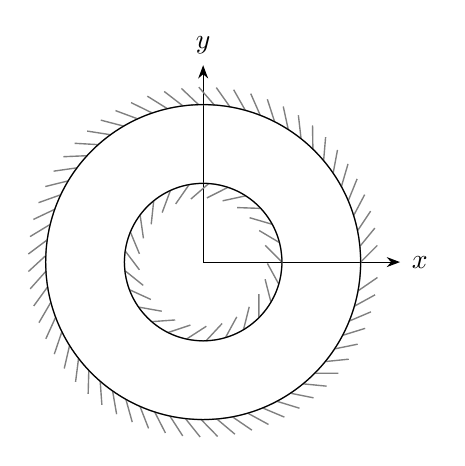
\begin{tikzpicture}[>=Stealth,scale=1.0, media/.style={font={\footnotesize\sffamily}}, interface/.style={postaction={draw,decorate,decoration={border,angle=-45, amplitude=0.3cm,segment length=2mm}}}]
      \draw[->](0,0) -- (2.5,0) node[pos=1.1]{$x$};
      \draw[->](0,0) -- (0,2.5) node[pos=1.1]{$y$};
      \draw[gray,line width=.5pt,interface] (0,0) circle(2cm);
      \draw [color=black] (0,0) circle(2cm);
      \draw[gray,line width=.5pt,interface/.style={postaction={draw,decorate,decoration={border,angle=45, amplitude=0.3cm,segment length=2.5mm}}}, interface] (0,0) circle(1cm);
      \draw [color=black] (0,0) circle(1cm);
    \end{tikzpicture}
  \end{center}
\end{figure}

\subsection{Rayleigh Problem: Stoke's First Problem}

Abrupt movement of a flat plate in fluid at rest.
Assuming parallel flow with no instabilities.

\begin{figure}[H]
  \begin{center}
    \begin{tikzpicture}[>=Stealth,scale=1.2, media/.style={font={\footnotesize\sffamily}}, interface/.style={postaction={draw,decorate,decoration={border,angle=-45, amplitude=0.3cm,segment length=2mm}}}]
      \draw[->](0,0) -- (5,0) node[pos=1.1]{$x$};
      \draw[->](0,0) -- (0,2.5) node[pos=1.1]{$y$};
      \draw[semithick, ->](1.25,-0.5) -- (2.75,-0.5) node[pos=1.2]{$U$};
      \draw[gray,line width=.5pt,interface](0,0)--(4.5,0);
      \draw[semithick] (0,0) -- (4.5,0);
      \draw[dotted] (1,0) -- (1,3);
      \draw (1,3) parabola[bend at end] (2,0);
    \end{tikzpicture}
  \end{center}
\end{figure}

\begin{empheq}[]{alignat*=3}
  &\mbox{\textbf{Steady:}} &\hspace{0.5in} \frac{\partial}{\partial{}t}=0 \\
  &\mbox{\textbf{Laminar or parallel flow:}} &\hspace{0.5in} v_{y}=v_{z}=0 \\
  &\mbox{\textbf{2-D flow:}} &\hspace{0.5in} \frac{\partial}{\partial{}z}=0 \\
  &\mbox{\textbf{Infinite plate:}} &\hspace{0.5in} \frac{\partial{}v_{x}}{\partial{}x}=0
\end{empheq}

Reducing the Navier-Stokes' equations as presented in component form on the handout by applying the simplifying assumptions listed above gives

\begin{equation*}
  \begin{split}
    \rho\frac{\partial{}v_{x}}{\partial{}t}&=\mu\frac{\partial^{2}v_{x}}{\partial{}y^{2}} \\
    0&=-\frac{\partial{}p}{\partial{}y}+\rho{}g_{y} \\
    0&=-\frac{\partial{}p}{\partial{}z}
  \end{split}
\end{equation*}

These equations can be rearranged to give

\begin{equation*}
  \begin{split}
    \frac{\partial{}v_{x}}{\partial{}t}&=\frac{\mu}{\rho}\frac{\partial^{2}v_{x}}{\partial{}y^{2}} \\
    0&=-\frac{\partial{}p}{\partial{}y}+\rho{}g_{y} \\
    0&=0
  \end{split}
\end{equation*}

The quantity $\frac{\mu}{\rho}=\nu$ is the dynamic viscosity, and we can simplify the first equation with this.
The second equation is just hydrostatic pressure in the $y$-direction.
So we want to solve the first equation.

\begin{empheq}[box=\roomyfbox]{equation*}
  \frac{\partial{}v_{x}}{\partial{}t}=\nu\frac{\partial^{2}v_{x}}{\partial{}y^{2}}
\end{empheq}

This is also known as the ``Heat Equation''.
So basically we have a PDE, but we want to make it an ODE somehow, so I guess we try to non-dimensionalize?

\subsubsection{Solution of Stokes' First Problem: Method 1}

\begin{equation*}
  f(\nu,y,t,\frac{v_{x}}{U})=0
\end{equation*}

\begin{equation*}
  \begin{split}
    \nu:&\;\frac{L^{2}}{T} \\
    y:&\;L \\
    t:&\;T \\
    \frac{v_{x}}{U}:&\;1
  \end{split}
\end{equation*}

and we have

\begin{equation*}
  \begin{split}
    n&=4 \\
    k&=2 \\
    j&=n-k=2
  \end{split}
\end{equation*}

Pick $y$ and $t$ to be the primary variables

\begin{equation*}
  \Pi_{1}=\nu{}y^{a}t^{b}
\end{equation*}

\begin{equation*}
  \left(\frac{L^{2}}{T}\right)L^{a}T^{b}=1
\end{equation*}

$a=-2$, $b=1$

\begin{empheq}[box=\roomyfbox]{equation*}
  \Pi_{1}=\frac{\nu{}t}{y^{2}}
\end{empheq}

However, we can make new Pi groups from any of the ``original'' Pi groups by operating on them by a function.
So, in this case it is convention (and simplifies the solution of the problem) if we pick the first Pi group instead to be

\begin{equation*}
  \Pi_{1}^{*}=\frac{y}{\sqrt{\nu{}t}}
\end{equation*}

However, while this simplifies the solution, we will show first the case using our original Pi group.
The second Pi group is

\begin{equation*}
  \Pi_{2}=\frac{v_{x}}{U}y^{c}t^{d}
\end{equation*}

\begin{equation*}
  1L^{c}T^{d}=1
\end{equation*}

$c=0$, $d=0$

\begin{empheq}[box=\roomyfbox]{equation*}
  \Pi_{2}=\frac{v_{x}}{U}
\end{empheq}

and so we have

\begin{empheq}[box=\roomyfbox]{equation*}
  \frac{v_{x}}{U}=\phi\left(\frac{\nu{}t}{y^{2}}\right)
\end{empheq}

or

\begin{equation*}
  v_{x}=U\phi\left(\frac{\nu{}t}{y^{2}}\right)
\end{equation*}

letting

\begin{empheq}[box=\roomyfbox]{equation*}
  \eta=\frac{\nu{}t}{y^{2}}
\end{empheq}

we have

\begin{equation*}
  v_{x}=U\phi(\eta)
\end{equation*}

Now we want to use this non-dimensionalized expression to help us solve the PDE, and reduce it to an ODE.\@

\begin{equation*}
  \frac{\partial{}v_{x}}{\partial{}t}=\nu\frac{\partial^{2}v_{x}}{\partial{}y^{2}}
\end{equation*}

So we need to evaluate using the function $\phi$ the following

\begin{equation*}
  \frac{\partial{}v_{x}}{\partial{}t}=U\frac{\partial\phi}{\partial\eta}\frac{\partial\eta}{\partial{}t}
\end{equation*}

\begin{equation*}
  \frac{\partial{}v_{x}}{\partial{}y}=U\frac{\partial\phi}{\partial\eta}\frac{\partial\eta}{\partial{}y}
\end{equation*}

\begin{equation*}
  \frac{\partial^{2}v_{x}}{\partial{}y^{2}}=U\left[\frac{\partial}{\partial{}y}\left(\frac{\partial\phi}{\partial\eta}\right)\frac{\partial\eta}{\partial{}y}+\frac{\partial\phi}{\partial\eta}\frac{\partial}{\partial{}y}\left(\frac{\partial\eta}{\partial{}y}\right)\right]
\end{equation*}

\begin{equation*}
  \frac{\partial^{2}v_{x}}{\partial{}y^{2}}=U\left[\frac{\partial^{2}\phi}{\partial\eta^{2}}\left(\frac{\partial\eta}{\partial{}y}\right)^{2}+\frac{\partial\phi}{\partial\eta}\frac{\partial^{2}\eta}{\partial{}y^{2}}\right]
\end{equation*}

And now we need to evaluate

\begin{equation*}
  \frac{\partial\eta}{\partial{}t}=\frac{\nu}{y^{2}}
\end{equation*}

\begin{equation*}
  \frac{\partial\eta}{\partial{}y}=-2\frac{\nu{}t}{y^{3}}
\end{equation*}

\begin{equation*}
  \frac{\partial^{2}\eta}{\partial{}y^{2}}=6\frac{\nu{}t}{y^{4}}
\end{equation*}

\begin{equation*}
  \left(\frac{\partial\eta}{\partial{}y}\right)^{2}=4\frac{\nu^{2}t^{2}}{y^{6}}
\end{equation*}

This gives

\begin{equation*}
  U\frac{\partial\phi}{\partial\eta}\frac{\partial\eta}{\partial{}t}=\nu{}U\left[\frac{\partial^{2}\phi}{\partial\eta^{2}}\left(\frac{\partial\eta}{\partial{}y}\right)^{2}+\frac{\partial\phi}{\partial\eta}\frac{\partial^{2}\eta}{\partial{}y^{2}}\right]
\end{equation*}

canceling out the $U$ and substituting in the known derivatives we get

\begin{equation*}
  \frac{\partial\phi}{\partial\eta}\frac{\nu}{y^{2}}=\nu{}\left[\frac{\partial^{2}\phi}{\partial\eta^{2}}\left(4\frac{\nu^{2}t^{2}}{y^{6}}\right)+\frac{\partial\phi}{\partial\eta}6\frac{\nu{}t}{y^{4}}\right]
\end{equation*}

\begin{equation*}
  \frac{\partial\phi}{\partial\eta}\left(\frac{\nu}{y^{2}}-6\nu\frac{\nu{}t}{y^{4}}\right)=\nu\frac{\partial^{2}\phi}{\partial\eta^{2}}\left(4\frac{\nu^{2}t^{2}}{y^{6}}\right)
\end{equation*}

\begin{equation*}
  \frac{\partial\phi}{\partial\eta}\left(\frac{y^{2}-6\nu{}t}{y^{2}}\right)=\frac{\partial^{2}\phi}{\partial\eta^{2}}\left(4\frac{\nu^{2}t^{2}}{y^{4}}\right)
\end{equation*}

\begin{equation*}
  \frac{\partial\phi}{\partial\eta}\left(1-6\eta\right)=\frac{\partial^{2}\phi}{\partial\eta^{2}}\left(4\eta^{2}\right)
\end{equation*}

\begin{equation*}
  \frac{\partial^{2}\phi}{\partial\eta^{2}}=\left(\frac{1-6\eta}{4\eta^{2}}\right)\frac{\partial\phi}{\partial\eta}
\end{equation*}

Now we separate and integrate twice

\begin{equation*}
  \frac{\frac{\partial^{2}\phi}{\partial\eta^{2}}}{\frac{\partial\phi}{\partial\eta}}=\frac{1-6\eta}{4\eta^{2}}
\end{equation*}

\begin{equation*}
  \frac{\frac{\partial}{\partial\eta}\frac{\partial\phi}{\partial\eta}}{\frac{\partial\phi}{\partial\eta}}=\frac{1-6\eta}{4\eta^{2}}
\end{equation*}

\begin{equation*}
  \int\frac{1}{\frac{\partial\phi}{\partial\eta}}\partial\left(\frac{\partial\phi}{\partial\eta}\right)=\int\frac{1-6\eta}{4\eta^{2}}\partial\eta
\end{equation*}

\begin{equation*}
  \int\frac{1}{\frac{\partial\phi}{\partial\eta}}\partial\left(\frac{\partial\phi}{\partial\eta}\right)=\frac{1}{4}\int\frac{1}{\eta^{2}}\partial\eta-\frac{6}{4}\int\frac{1}{\eta}\partial\eta
\end{equation*}

\begin{equation*}
  \ln\left(\frac{\partial\phi}{\partial\eta}\right)=-\frac{1}{4\eta}-\frac{6}{4}\ln(\eta)+f_{1}(\text{not }\eta)
\end{equation*}

\begin{equation*}
  \frac{\partial\phi}{\partial\eta}=\text{exp}\left(-\frac{1}{4\eta}-\frac{6}{4}\ln(\eta)+C_{1}\right)
\end{equation*}

\begin{equation*}
  \int\partial\phi=\int\text{exp}\left(-\frac{1}{4\eta}-\frac{6}{4}\ln(\eta)+C_{1}\right)\partial\eta
\end{equation*}

\begin{equation*}
  \phi=C_{2}\int_{0}^{\eta}\text{exp}\left(-\frac{1}{4\eta}-\frac{6}{4}\ln(\eta)\right)\partial\eta+C_{3}
\end{equation*}

Evaluate this integral to get

\begin{equation*}
  \phi=C_{2}\left[-2\sqrt{\pi}\text{erf}\left(\frac{1}{2\sqrt{\eta}}\right)\right]_{0}^{\eta}+C_{3}
\end{equation*}

\begin{equation*}
  \phi=2\sqrt{\pi}C_{2}\left[1-\text{erf}\left(\frac{1}{2\sqrt{\eta}}\right)\right]+C_{3}
\end{equation*}

 Now apply boundary conditions to determine $C_{2}$ and $C_{3}$.
 Looking at $\eta$ in terms of $y$ we have

\begin{equation*}
  y\rightarrow\infty\Rightarrow\eta\rightarrow0\;and\;\frac{v_{x}(y\rightarrow\infty)}{U}=0\Rightarrow\phi(\eta=0)=0
\end{equation*}

\begin{equation*}
  y=0\Rightarrow\eta=\infty\;and\;\frac{v_{x}(y=0)}{U}=1\Rightarrow\phi(\eta=\infty)=1
\end{equation*}

Continuing to apply these boundary conditions, with the following

\begin{equation*}
  \text{erf}(0)=0
\end{equation*}

\begin{equation*}
  \text{erf}(\infty)=1
\end{equation*}

First boundary condition $\eta=0$

\begin{equation*}
  0=2\sqrt{\pi}C_{2}\left[1-\text{erf}(\infty)\right]+C_{3}
\end{equation*}

\begin{equation*}
  C_{3}=0
\end{equation*}

Next boundary condition $\eta\rightarrow\infty$

\begin{equation*}
  1=2\sqrt{\pi}C_{2}\left[1-\text{erf}(0)\right]+C_{3}
\end{equation*}

\begin{equation*}
  1=2\sqrt{\pi}C_{2}
\end{equation*}

\begin{equation*}
  C_{2}=\frac{1}{2\sqrt{\pi}}
\end{equation*}

\begin{equation*}
  \phi(\eta)=\left[-\text{erf}\left(\frac{1}{2\sqrt{\eta}}\right)\right]_{0}^{\eta}
\end{equation*}

\begin{equation*}
  \phi(\eta)=\left[-\text{erf}\left(\frac{1}{2\sqrt{\eta}}\right)+\text{erf}(\infty)\right]
\end{equation*}

\begin{empheq}[box=\roomyfbox]{equation*}
  \phi(\eta)=\left[1-\text{erf}\left(\frac{1}{2\sqrt{\eta}}\right)\right]
\end{empheq}

Now relate this function with the non-dimensional variables, or Pi groups, back to the physical variables

\begin{equation*}
  \frac{v_{x}(y,t)}{U}=\left[1-\text{erf}\left(\frac{1}{2\sqrt{\frac{\nu{}t}{y^{2}}}}\right)\right]
\end{equation*}

\begin{empheq}[box=\fboxTwo]{alignat*=3}
  &\mbox{\textbf{Velocity for Stokes' first problem:}} &\hspace{0.5in} \frac{v_{x}(y,t)}{U}=\left[1-\text{erf}\left(\frac{y}{2\sqrt{\nu{}t}}\right)\right]
\end{empheq}

Now, if at the beginning we had picked a different non dimensional variable, or Pi group, $\eta$ the result would have been the same, but the solution would have been easier, in particular in the evaluation of the integral that resulted in the error function.
Some extra stuff.
Look at the dimensional analysis sheet and see that the time scale for the diffusion of viscous effects into the fluid are like
\begin{equation*}
  t_{c}\sim\frac{L^{2}}{\nu}
\end{equation*}
and we need to pick a characteristic length scale, which is usually the boundary layer thickness $\delta$.
This gives
\begin{equation*}
  t_{c}\sim\frac{\delta^{2}}{\nu}
\end{equation*}
Solving for $\delta$ we have
\begin{equation*}
  \delta\sim\sqrt{\nu{}t}
\end{equation*}
And we can approximate the shear stress as a linear velocity profile over the boundary layer
\begin{equation*}
  \tau_{w}\sim\frac{\mu{}U}{\delta}\sim\frac{\mu{}U}{\sqrt{\nu{}t}}
\end{equation*}

\subsubsection{Solution of Stokes' First Problem: Method 2}

Using different $\eta$

\subsection{Stokes' Second Problem}

Stokes apparently had many problems.
In this problem, at first I thought we could just reuse most of the solution from Stokes' first problem, but change the boundary condition and somehow take into account the oscillating boundary condition because the constants of integration that we found last time are not actually constants, but functions of not eta.
Should clear up the notation on how to express arbitrary constants that are ``not a function'' of some variable.
This didn't work though, and I think it is something like we fundamentally ignored the variable omega (plate oscillation frequency) when we non-dimensionalized, so our solution won't work.
This basically means the whole non-dimensionalizing part to turn the governing PDE into an ODE needs to be redone.

\begin{figure}[H]
  \begin{center}
    \begin{tikzpicture}[>=Stealth,scale=1.2, media/.style={font={\footnotesize\sffamily}}, interface/.style={postaction={draw,decorate,decoration={border,angle=-45, amplitude=0.3cm,segment length=2mm}}}]
      \draw[->](0,0) -- (5,0) node[pos=1.1]{$x$};
      \draw[->](0,0) -- (0,2.5) node[pos=1.1]{$y$};
      \draw[semithick, <->](1.25,-0.5) -- (2.75,-0.5) node[pos=1.4]{$U\cos{\omega t}$};
      \draw[gray,line width=.5pt,interface](0,0)--(4.5,0);
      \draw[semithick] (0,0) -- (4.5,0);
      \draw[dotted] (1,0) -- (1,3);
      \draw (1,3) parabola[bend at end] (2,0);
    \end{tikzpicture}
  \end{center}
\end{figure}

\begin{example}
  \textbf{Viscometer}
  A motor with a  cylinder attached is submerged in a viscous fluid.
  The motor is set to rotate at a known rpm, and a device is used to measure the torque required to rotate the cylinder.
  From this, we can figure out the viscosity of the fluid.
\end{example}

\section{Nondimensionalizing the Navier-Stokes' Equation}

By nondimensionalizing the Navier-Stokes' Equations, we can understand better what contributions like viscosity are ``large'' or ``small''.
To express in dimensionless variables, we have to scale all the variables in the problem using characteristic scales for the problem of interest.

\begin{equation*}
  \underline{x}^{*}=\frac{\underline{x}}{l}
  \hspace{0.4in}
  \underline{v}^{*}=\frac{\underline{v}}{V}
  \hspace{0.4in}
  p^{*}=\frac{p}{\rho{}V^{2}}
  \hspace{0.4in}
  t^{*}=\frac{t}{\left(\frac{l}{V}\right)}=\frac{Vt}{l}
\end{equation*}
solving

\begin{equation*}
  \underline{x}=\underline{x}^{*}l
  \hspace{0.4in}
  \underline{v}=\underline{v}^{*}V
  \hspace{0.4in}
  p=p^{*}\rho{}V^{2}
  \hspace{0.4in}
  t=\frac{lt^{*}}{V}
\end{equation*}
Where the time is called the convective time scale.
And the del operator $\underline{\nabla}$ takes a different form when nondimensionalized as well.

\begin{equation*}
  \begin{split}
    \underline{\nabla}&=
    \begin{bmatrix}
    \frac{\partial}{\partial{}x} &
    \frac{\partial}{\partial{}y} &
    \frac{\partial}{\partial{}z}
    \end{bmatrix} \\
    &=
    \begin{bmatrix}
    \frac{\partial}{\partial(x^{*}l)} &
    \frac{\partial}{\partial(y^{*}l)} &
    \frac{\partial}{\partial(z^{*}l)}
    \end{bmatrix} \\
    &=
    \frac{1}{l}
    \begin{bmatrix}
    \frac{\partial}{\partial{}x^{*}} &
    \frac{\partial}{\partial{}y^{*}} &
    \frac{\partial}{\partial{}z^{*}}
    \end{bmatrix} \\
    &=\frac{1}{l}\underline{\nabla}^{*}
  \end{split}
\end{equation*}
The Navier-Stokes' Equation is

\begin{equation*}
  \rho\left(\frac{\partial\underline{v}}{\partial{}t}+\underline{v}\cdot\underline{\nabla}\underline{v}\right)=-\underline{\nabla}p+\mu\nabla^{2}\underline{v}+\rho\underline{g}
\end{equation*}

\begin{equation*}
  \rho\left(\frac{\partial(\underline{v}^{*}V)}{\partial(\frac{lt^{*}}{V})}+(\underline{v}^{*}V)\cdot\frac{1}{l}\underline{\nabla}^{*}(\underline{v}^{*}V)\right)=-\frac{1}{l}\underline{\nabla}^{*}(p^{*}\rho{}V^{2})+\frac{\mu}{l^{2}}\nabla^{*2}(\underline{v}^{*}V)+\rho\underline{g}
\end{equation*}

\begin{equation*}
  \rho\left(\frac{V^{2}}{l}\frac{\partial\underline{v}^{*}}{\partial{}t^{*}}+\frac{V^{2}}{l}\underline{v}^{*}\cdot\underline{\nabla}^{*}\underline{v}^{*}\right)=-\frac{\rho{}V^{2}}{l}\underline{\nabla}^{*}p^{*}+\frac{\mu{}V}{l^{2}}\nabla^{*2}\underline{v}^{*}+\rho\underline{g}
\end{equation*}
Divide through by $\rho\frac{V^{2}}{l}$ and get

\begin{equation*}
  \frac{\partial\underline{v}^{*}}{\partial{}t^{*}}+\underline{v}^{*}\cdot\underline{\nabla}^{*}\underline{v}^{*}=-\underline{\nabla}^{*}p^{*}+\underbrace{\left(\frac{\mu}{\rho{}Vl}\right)}_{\frac{1}{\text{Re}}}\nabla^{*2}\underline{v}^{*}+\underbrace{\left(\frac{gl}{V^{2}}\right)}_{\frac{1}{\text{Fr}^{2}}}\underline{\hat{e}}_{z}
\end{equation*}

The Froude number plays an analogous role to the Mach number in a compressible flow.
From this non-dimensionalized version of Navier-Stokes' Equation, we can see if $\text{Re}=\frac{\rho{}Vl}{\mu}$ is very large, the viscous terms in the equation of motion become very small and negligible compared to the inertial terms in the equation.
The \textit{flow} is inviscid, not the \textit{fluid}.

\begin{equation*}
  \frac{\partial\underline{v}^{*}}{\partial{}t^{*}}+\underline{v}^{*}\cdot\underline{\nabla}^{*}\underline{v}^{*}=-\underline{\nabla}^{*}p^{*}+\frac{1}{\text{Re}}\nabla^{*2}\underline{v}^{*}+\frac{gl}{V^{2}}\underline{\hat{e}}_{z}
\end{equation*}

\begin{equation*}
  \frac{D\underline{v}^{*}}{Dt^{*}}=-\underline{\nabla}^{*}p^{*}+\frac{1}{\text{Re}}\nabla^{*2}\underline{v}^{*}+\frac{gl}{V^{2}}\underline{\hat{e}}_{z}
\end{equation*}

\begin{equation*}
  \frac{D\underline{v}^{*}}{Dt^{*}}=-\underline{\nabla}^{*}p^{*}+\frac{1}{\text{Re}}\nabla^{*2}\underline{v}^{*}+\frac{1}{\text{Fr}^{2}}\underline{\hat{e}}_{z}
\end{equation*}

% TODO@dpwiese - See lecture notes from Tuesday 10-22 to finish this.
To solve such problems, use the following procedure.
Nondimensionalize the problem we are interested in: the skinny gap considered for lubrication theory problems.
Do this just like all the other dimensional analysis problems before.
Take those non dimensional quantities or Pi groups and make new ones just so they look like one we are familiar with.
Write a few inequalities based on the prescribed geometry.
That is: $h<<L$ and $\frac{dh}{dx}<<1$ which says gap is small and doesn't expand too quickly.
Solve for the dimensional variables in terms of the nondomensional ones.
Plug these dimensional variables into NSE and obtain a non dimensionalized version of the equation.
From this equation and using our assumptions of flow geometry, we can simplify terms within the non dimensional NSE.\@

\begin{itemize}
  \item{why in lubrication theory can we show that inertia effects are small?}
  \item{How do we say that two non dimensional derivatives are of the same order of magnitude? To allow us to compare terms like mckinley did in notes comparing 5/6\ldots}
  \item{integration of multivariable functions required for the solution to Stokes' first problem $f(not z)$}
  \item{Stokes flow from original nondimensionalization (see sphere moving in fluid example below) and in general how to ignore inertial effects? $\rho=0$?}
\end{itemize}

\chapter{Dimensional Analysis}

To solve a dimensional analysis problem, use the following steps.

\begin{enumerate}
  \item{Pick the fundamental variables which describe the problem, and note the number $n$ of these fundamental variables}
  \begin{itemize}
    \item{In picking the fundamental variables, we typically want to pick one quantity which describe the fluid, the flow, and the geometry.}
  \end{itemize}
  \item{Write the fundamental dimensions for each fundamental variable, and note the number $k$ of independent fundamental dimensions.}
  \item{%
    Subtracting $j=n-k$ we need $j$ Pi groups.
    We need to pick $k$ primary variables to use in making these Pi groups.
  }
  \item{Make the $j$ Pi groups}
  \item{Identify as many of the Pi groups as known dimensionless quantities, such as Reynolds number, Weber number, etc.}
\end{enumerate}

% TODO@dpwiese - clearpage to suppress underfilled hbox warning
\clearpage
\begin{example}
  \textbf{Sphere falling in a viscous fluid}
  \begin{center}
    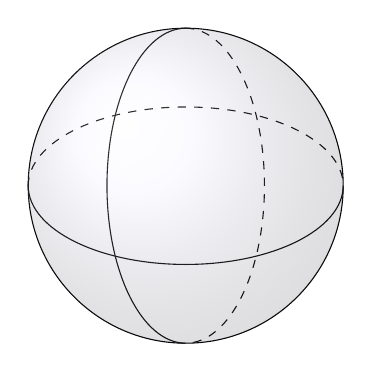
\begin{tikzpicture}[scale=2.0]
      \draw (-1,0) arc (180:360:1cm and 0.5cm);
      \draw[dashed] (-1,0) arc (180:0:1cm and 0.5cm);
      \draw (0,1) arc (90:270:0.5cm and 1cm);
      \draw[dashed] (0,1) arc (90:-90:0.5cm and 1cm);
      \draw (0,0) circle (1cm);
      \shade[ball color=blue!10!white,opacity=0.20] (0,0) circle (1cm);
    \end{tikzpicture}
  \end{center}
  Fundamental variables $F_{D}$, $U$, $\rho$, $\mu$, $D$
  $n=5$.
  Fundamental dimensions are
  \begin{equation*}
    \begin{split}
      F_{D}:&\;\frac{ML}{T^{2}} \\
      U:&\;\frac{L}{T} \\
      \rho:&\;\frac{M}{L^{3}} \\
      \mu:&\;\frac{M}{LT} \\
      D:&\;L
    \end{split}
  \end{equation*}
  From this we see that the number of independent dimensions is $k=3$.
  So $n-k=2$ and we need $2$ Pi groups.
  Choose $\rho$, $U$, and $D$ as the primary variables.
  \begin{equation*}
    \Pi_{1}=F_{D}\rho^{a}U^{b}D^{c}
    \hspace{0.5in}
    \Pi_{2}=\mu\rho^{d}U^{e}D^{f}
  \end{equation*}
  \begin{equation*}
    \begin{split}
      &\left(\frac{ML}{T^{2}}\right)\left(\frac{M}{L^{3}}\right)^{a}\left(\frac{L}{T}\right)^{b}\left(L\right)^{c}=M^{0}L^{0}T^{0} \\
      &\left(\frac{M}{LT}\right)\left(\frac{M}{L^{3}}\right)^{d}\left(\frac{L}{T}\right)^{e}\left(L\right)^{f}=M^{0}L^{0}T^{0}
    \end{split}
  \end{equation*}
  \begin{equation*}
    T^{-2}T^{-b}=T^{0}
    \hspace{0.5in}
    T^{-1}T^{-f}=T^{0}
  \end{equation*}
  \begin{equation*}
    MM^{a}=M^{0}
    \hspace{0.5in}
    MM^{d}=M^{0}
  \end{equation*}
  \begin{equation*}
    LL^{-3a}L^{b}L^{c}=L^{0}
    \hspace{0.5in}
    L^{-1}L^{-3d}L^{e}L^{f}=L^{0}
  \end{equation*}
  \begin{equation*}
    b=-2
    \hspace{0.5in}
    f=-1
  \end{equation*}
  \begin{equation*}
    a=-1
    \hspace{0.5in}
    d=-1
  \end{equation*}
  \begin{equation*}
    LL^{3}L^{-2}L^{c}=L^{0}
    \hspace{0.5in}
    L^{-1}L^{3}L^{e}L^{-1}=L^{0}
  \end{equation*}
  \begin{equation*}
    c=-2
    \hspace{0.5in}
    e=-1
  \end{equation*}
  \begin{equation*}
    \Pi_{1}=F_{D}\rho^{-1}U^{-2}D^{-2}
    \hspace{0.5in}
    \Pi_{2}=\mu\rho^{-1}U^{-1}D^{-1}
  \end{equation*}
  \begin{equation*}
    \Pi_{1}=\frac{F_{D}}{\rho{}D^{2}U^{2}}
    \hspace{0.5in}
    \Pi_{2}=\frac{\mu}{\rho{}DU}=\frac{1}{\text{Re}}
  \end{equation*}
  $\Pi_{1}$ is essentially the drag coefficient.
  Since we know the Pi groups can always be off by a constant factor, the drag coefficient usually looks like
  \begin{equation*}
    C_{D}=\frac{F_{d}}{\frac{1}{2}\rho{}U^{2}A}
  \end{equation*}
  where $A$ is the projected area.
  And we can see that
  \begin{equation*}
    \Pi_{1}=\phi\left(\Pi_{2}\right)
  \end{equation*}
  \begin{equation*}
    C_{D}=\phi\left(\frac{1}{\text{Re}}\right)
  \end{equation*}
  And when the Reynolds number is very large, inertia dominates and viscous forces are negligible.
  In this case, we can redo the dimensional analysis, but this time without $\mu$.
  This gives $n=4$, but with $k=3$ still, and so there is only one Pi group.
  In this case we know that that one Pi group, which is shown below, must be a constant.
  \begin{empheq}[]{alignat*=3}
    &\mbox{\textbf{High Re:}} &\hspace{0.5in} \frac{F_{D}}{\rho{}U^{2}D^{2}}=\text{constant}
  \end{empheq}
  What about when Reynolds number is very very small?
  Essentially this means inertia is negligible, so that means $\rho$ is small?
  \begin{empheq}[]{alignat*=3}
    &\mbox{\textbf{Low Re:}} &\hspace{0.5in} \frac{F_{D}}{xyz}=\text{constant}
  \end{empheq}
  Basically the drag coefficient is given as a dimensionless drag force.
  So take the drag force and divide it by something that has units of force.
  To get a force we do pressure times area, so depending on whether viscous or inertial pressure dominates, pick the correct one, multiply it by an area, and we have a force.
  \begin{empheq}[]{alignat*=3}
    &\mbox{\textbf{High Re:}} &\hspace{0.5in} C_{D}=\text{const}\frac{F_{D}}{\rho{}U^{2}D^{2}}
  \end{empheq}
  \begin{empheq}[]{alignat*=3}
    &\mbox{\textbf{Low Re:}} &\hspace{0.5in} C_{D}=\text{const}\frac{F_{D}}{\frac{\mu{}U}{R}R^{2}}
  \end{empheq}
  so the drag forces in each of these cases are
  \begin{empheq}[]{alignat*=3}
    &\mbox{\textbf{High Re:}} &\hspace{0.5in} F_{D}=\text{const}\rho{}U^{2}D^{2}
  \end{empheq}
  \begin{empheq}[]{alignat*=3}
    &\mbox{\textbf{Low Re:}} &\hspace{0.5in} F_{D}=\text{const}\mu{}UR
  \end{empheq}
\end{example}

The drag on a sphere\ldots when viscosity negligible:

\begin{equation*}
  F_{D}=K_{2}\rho{}v^{2}R^{2}
\end{equation*}

when inertia is negligible

\begin{equation*}
  F_{D}=K_{3}\mu{}vR
\end{equation*}

\textbf{Stokes Creeping Flow}

Can get the following equations by simplifying and solving Navier-Stokes' equations.

\begin{equation*}
  v_{r}=-V\cos(\theta)\left(1-\frac{3R}{2r}+\frac{R^{3}}{2r^{3}}\right)
\end{equation*}

\begin{equation*}
  v_{\theta}=V\sin(\theta)\left(1-\frac{3R}{4r}+\frac{R^{3}}{4r^{3}}\right)
\end{equation*}

\begin{equation*}
  p=p_{\infty}-\frac{3}{2}\left(\frac{\mu{}v}{R}\right)\frac{R^{2}}{r^{2}}\cos(\theta)
\end{equation*}

To find the drag force on a sphere, need the pressure gradient and the shear stress at the surface, $\tau_{r\theta}$ and integrate all the terms over the surface of a sphere

\begin{empheq}[box=\fboxTwo]{alignat*=3}
  &\mbox{\textbf{Stokes drag on a sphere}} \hspace{0.5in}& \underline{F}_{D,x}=\int_{A}\underline{e}_{x}\cdot\uuline{\tau}dA=6\pi\mu{}RV=3\pi\mu{}VD
\end{empheq}

and so $C_{D}$ of the sphere simplifies to

\begin{equation*}
  C_{D}=\frac{24}{\text{Re}}
\end{equation*}

\begin{example}
  How long for a falling sphere to get to steady state velocity?
\end{example}

\chapter{Lubrication Theory}

The key requirement for lubrication theory is that the ratio $h/l<<1$ is small, where $h$ is gap between surfaces and $L$ is the length.
More than one readily identifiable characteristic length scale.
If there is a clear separation of scales $h<<l$ then we can use lubrication analysis to simplify the Navier-Stokes' equation.
(Slender body analysis).

\section{Cartesian Coordinates}

\begin{equation*}
  \underline{x}^{*}=\frac{\underline{x}}{l}
  \hspace{0.4in}
  \underline{y}^{*}=\frac{\underline{y}}{h}
  \hspace{0.4in}
  \underline{v}_{x}^{*}=\frac{\underline{v}_{x}}{U}
  \hspace{0.4in}
  \underline{v}_{y}^{*}=\frac{\underline{v}_{y}}{V_{c}}
  \hspace{0.4in}
  t^{*}=\frac{t}{t_{c}}
\end{equation*}

\begin{equation*}
  p^{*}=\frac{p}{p_{c}}
  \hspace{0.4in}
  p^{*}=\frac{p}{\rho{}V^{2}}
  \hspace{0.4in}
  t^{*}=\frac{t}{\left(\frac{l}{V}\right)}=\frac{Vt}{l}
\end{equation*}

where $V_{c}$ is a characteristic velocity.
Solving for the dimensional quantities in terms of the dimensionless ones, we have

\begin{equation*}
  \underline{x}=\underline{x}^{*}l
  \hspace{0.4in}
  \underline{y}=\underline{y}^{*}h
  \hspace{0.4in}
  \underline{v}_{x}=\underline{v}_{x}^{*}U
  \hspace{0.4in}
  \underline{v}_{y}=\underline{v}_{y}^{*}V_{c}
  \hspace{0.4in}
  t=t^{*}t_{c}
  \hspace{0.4in}
  p=p^{*}p_{c}
\end{equation*}

\subsection{Non-dimensionalization of Conservation of Mass}

Starting with conservation of mass for 2-D in cartesian coordinates
\begin{equation*}
  \frac{\partial{}v_{x}}{\partial{}x}+\frac{\partial{}v_{y}}{\partial{}y}=0
\end{equation*}
we substitute these into conservation of mass and get
\begin{equation*}
  \frac{\partial(v_{x}^{*}U)}{\partial(x^{*}l)}+\frac{\partial(v_{y}^{*}V_{c})}{\partial(y^{*}h)}=0
\end{equation*}
Pulling out the characteristic terms we have
\begin{equation*}
  \frac{U}{l}\frac{\partial{}v_{x}^{*}}{\partial{}x^{*}}+\frac{V_{c}}{h}\frac{\partial{}v_{y}^{*}}{\partial{}y^{*}}=0
\end{equation*}
and so from this both of the dimensionless groups are are order one dimensionless quantities, and so we see that the characteristic velocity must scale as
\begin{empheq}[box=\roomyfbox]{equation*}
  V_{c}\sim\frac{Uh}{l}
\end{empheq}

\subsection{Simplification of Navier-Stokes for Lubrication Theory}

\subsubsection{$x$-direction}

The $x$-component of the Navier-Stokes equation in cartesian coordinates is the following

\begin{equation*}
  \rho\left(\frac{\partial{}v_{x}}{\partial{}t}+v_{x}\frac{\partial{}v_{x}}{x}+v_{y}\frac{\partial{}v_{x}}{\partial{}y}+v_{z}\frac{\partial{}v_{x}}{\partial{}z}\right)=\mu\left[\frac{\partial^{2}v_{x}}{\partial{}x^{2}}+\frac{\partial^{2}v_{x}}{\partial{}y^{2}}+\frac{\partial^{2}v_{x}}{\partial{}z^{2}}\right]-\frac{\partial{}p}{\partial{}x}+\rho{}g_{x}
\end{equation*}
Simplifying these equations for 2-D flow, we get

\begin{equation*}
  \rho\left(\frac{\partial{}v_{x}}{\partial{}t}+v_{x}\frac{\partial{}v_{x}}{x}+v_{y}\frac{\partial{}v_{x}}{\partial{}y}\right)=\mu\left[\frac{\partial^{2}v_{x}}{\partial{}x^{2}}+\frac{\partial^{2}v_{x}}{\partial{}y^{2}}\right]-\frac{\partial{}p}{\partial{}x}+\rho{}g_{x}
\end{equation*}
Substituting in the dimensional variables in terms of the non dimensional variables and characteristic values, we get

\begin{equation*}
  \rho\left(\frac{\partial(v_{x}^{*}U)}{\partial(t^{*}t_{c})}+v_{x}^{*}U\frac{\partial(v_{x}^{*}U)}{\partial(x^{*}l)}+v_{y}^{*}V\frac{\partial(v_{x}^{*}U)}{\partial(y^{*}h)}\right)=\mu\left[\frac{\partial^{2}(v_{x}^{*}U)}{\partial(x^{*}l)^{2}}+\frac{\partial^{2}(v_{x}^{*}U)}{\partial{}(y^{*}h)^{2}}\right]-\frac{\partial(p^{*}p_{c})}{\partial(x^{*}l)}+\rho{}g_{x}
\end{equation*}
Pull out characteristic values to leave differential equation in dimensionless form

\begin{equation*}
  \rho\biggr(\frac{U}{t_{c}}\frac{\partial{}v_{x}^{*}}{\partial{}t^{*} }+\frac{U^{2}}{l}v_{x}^{*}\frac{\partial{}v_{x}^{*}}{\partial{}x^{*}}+\frac{VU}{h}v_{y}^{*}\frac{\partial{}v_{x}^{*}}{\partial{}y^{*}}\biggr)=\mu\biggr[\frac{U}{l^{2}}\frac{\partial^{2}v_{x}^{*}}{\partial{}x^{*2}}+\frac{U}{h^{2}}\frac{\partial^{2}v_{x}^{*}}{\partial{}y^{*2}}\biggr]-\frac{p_{c}}{l}\frac{\partial{}p^{*}}{\partial{}x^{*}}+\rho{}g_{x}
\end{equation*}
Plug in the scaling for $V$ which came from continuity and dividing by $\mu$

\begin{equation*}
  \frac{\rho}{\mu}\biggr(\frac{U}{t_{c}}\frac{\partial{}v_{x}^{*}}{\partial{}t^{*} }+\frac{U^{2}}{l}v_{x}^{*}\frac{\partial{}v_{x}^{*}}{\partial{}x^{*}}+\frac{U^{2}}{l}v_{y}^{*}\frac{\partial{}v_{x}^{*}}{\partial{}y^{*}}\biggr)=\biggr[\frac{U}{l^{2}}\frac{\partial^{2}v_{x}^{*}}{\partial{}x^{*2}}+\frac{U}{h^{2}}\frac{\partial^{2}v_{x}^{*}}{\partial{}y^{*2}}\biggr]-\frac{p_{c}}{\mu{}l}\frac{\partial{}p^{*}}{\partial{}x^{*}}+\frac{\rho}{\mu}g_{x}
\end{equation*}
Multiply both sides by $\frac{h^{2}}{U}$

\begin{equation*}
  \frac{\rho{}h^{2}}{\mu{}t_{c}}\frac{\partial{}v_{x}^{*}}{\partial{}t^{*} }+\frac{\rho{}Uh^{2}}{\mu{}l}v_{x}^{*}\frac{\partial{}v_{x}^{*}}{\partial{}x^{*}}+\frac{\rho{}Uh^{2}}{\mu{}l}v_{y}^{*}\frac{\partial{}v_{x}^{*}}{\partial{}y^{*}}=\frac{h^{2}}{l^{2}}\frac{\partial^{2}v_{x}^{*}}{\partial{}x^{*2}}+\frac{\partial^{2}v_{x}^{*}}{\partial{}y^{*2}}-\frac{h^{2}p_{c}}{\mu{}Ul}\frac{\partial{}p^{*}}{\partial{}x^{*}}+\frac{h^{2}\rho}{\mu{}U} g_{x}
\end{equation*}
Notice now that to keep the left side of the same order, we must pick the characteristic time as

\begin{equation*}
  t_{c}=\frac{l}{U}
\end{equation*}
Substituting this in to get

\begin{equation*}
  \frac{\rho{}Uh^{2}}{\mu{}l}\frac{\partial{}v_{x}^{*}}{\partial{}t^{*} }+\frac{\rho{}Uh^{2}}{\mu{}l}v_{x}^{*}\frac{\partial{}v_{x}^{*}}{\partial{}x^{*}}+\frac{\rho{}Uh^{2}}{\mu{}l}v_{y}^{*}\frac{\partial{}v_{x}^{*}}{\partial{}y^{*}}=\frac{h^{2}}{l^{2}}\frac{\partial^{2}v_{x}^{*}}{\partial{}x^{*2}}+\frac{\partial^{2}v_{x}^{*}}{\partial{}y^{*2}}-\frac{h^{2}p_{c}}{\mu{}Ul}\frac{\partial{}p^{*}}{\partial{}x^{*}}+\frac{h^{2}\rho}{\mu{}U}g_{x}
\end{equation*}
Recognize the Reynolds number terms

\begin{equation*}
  \text{Re}_{l}\frac{h^{2}}{l^{2}}\left(\frac{\partial{}v_{x}^{*}}{\partial{}t^{*} }+v_{x}^{*}\frac{\partial{}v_{x}^{*}}{\partial{}x^{*}}+v_{y}^{*}\frac{\partial{}v_{x}^{*}}{\partial{}y^{*}}\right)=\frac{h^{2}}{l^{2}}\frac{\partial^{2}v_{x}^{*}}{\partial{}x^{*2}}+\frac{\partial^{2}v_{x}^{*}}{\partial{}y^{*2}}-\frac{h^{2}p_{c}}{\mu{}Ul}\frac{\partial{}p^{*}}{\partial{}x^{*}}+\frac{h^{2}\rho}{\mu{}U}g_{x}
\end{equation*}
If $\text{Re}_{l}\frac{h^{2}}{l^{2}}<<1$ and $\frac{h^{2}}{l^{2}}<<1$ then we can simplify this expression

\begin{equation*}
  0=\frac{\partial^{2}v_{x}^{*}}{\partial{}y^{*2}}-\frac{h^{2}p_{c}}{\mu{}Ul}\frac{\partial{}p^{*}}{\partial{}x^{*}}+\frac{h^{2}\rho}{\mu{}U}g_{x}
\end{equation*}
Rearranging terms we can redimensionalize

\begin{equation*}
  0=\frac{\mu{}U}{h^{2}}\frac{\partial^{2}v_{x}^{*}}{\partial{}y^{*2}}-\frac{p_{c}}{l}\frac{\partial{}p^{*}}{\partial{}x^{*}}+\rho{}g_{x}
\end{equation*}

\begin{equation*}
  \mu\frac{\partial^{2}(Uv_{x}^{*})}{\partial(hy^{*2})}-\frac{\partial(p_{c}p^{*})}{\partial(lx^{*})}+\rho{}g_{x}=0
\end{equation*}
So the governing equation of motion for lubrication theory in the $x$-direction is the following, where $g_{x}$ is the component of gravity along the $x$-axis.

\begin{empheq}[box=\fboxTwo]{alignat*=3}
  &\mbox{\textbf{Lubrication theory $x$-direction:}} &\hspace{0.5in} \mu\frac{\partial^{2}v_{x}}{\partial^{2}}-\frac{\partial{}p}{\partial{}x}+\rho{}g_{x}=0
\end{empheq}

We can now separate this equation and integrate it back to obtain an expression for the velocity.
However, we require two boundary conditions, and these depend on the problem being solved.
A free surface corresponds to Neumann boundary conditions, those where the shear stress at the free surface are zero, and so the relationship of velocity and shear stress says that the derivative of the velocity with respect to the perpendicular direction are zero.
Will clear this up later.
Dirichlet boundary conditions are those where the velocity itself takes a certain value rather than derivative.
Integrate the governing equation back.

\begin{equation*}
  \mu\int d\frac{dv_{x}}{dy}=\int\left(\frac{\partial{}p}{\partial{}x}-\rho{}g_{x}\right)dy
\end{equation*}

\begin{equation*}
  \mu\frac{dv_{x}}{dy}=\left(\frac{\partial{}p}{\partial{}x}-\rho{}g_{x}\right)y+C_{1}
\end{equation*}

\begin{equation*}
  \mu\int dv_{x}=\int\left(\frac{\partial{}p}{\partial{}x}-\rho{}g_{x}\right)ydy+\int C_{1}dy
\end{equation*}

\begin{equation*}
  \mu{}v_{x}=\frac{1}{2}\left(\frac{\partial{}p}{\partial{}x}-\rho{}g_{x}\right)y^{2}+C_{1}y+C_{2}
\end{equation*}

\subsubsection{$y$-direction}

Taking the Navier-Stokes equation in the $y$-direction and substituting in the dimensional terms we have
\begin{equation*}
  \rho\left(\frac{\partial(v_{y}^{*}V)}{\partial(t^{*}t_{c})}+v_{x}^{*}U\frac{\partial(v_{y}^{*}V)}{\partial(x^{*}l)}+v_{y}^{*}V\frac{\partial(v_{y}^{*}V)}{\partial(y^{*}h)}\right)=\mu\left[\frac{\partial^{2}(v_{y}^{*}V)}{\partial(x^{*}l)^{2}}+\frac{\partial^{2}(v_{y}^{*}V)}{\partial{}(y^{*}h)^{2}}\right]-\frac{\partial(p^{*}p_{c})}{\partial(y^{*}h)}+\rho{}g_{y}
\end{equation*}
Pulling out the characteristic values so the derivatives are dimensionless
\begin{equation*}
  \rho\biggr(\frac{V}{t_{c}}\frac{\partial{}v_{y}^{*}}{\partial{}t^{*} }+\frac{UV}{l}v_{x}^{*}\frac{\partial{}v_{y}^{*}}{\partial{}x^{*}}+\frac{V^{2}}{h}v_{y}^{*}\frac{\partial{}v_{y}^{*}}{\partial{}y^{*}}\biggr)=\mu\biggr[\frac{V}{l^{2}}\frac{\partial^{2}v_{y}^{*}}{\partial{}x^{*2}}+\frac{V}{h^{2}}\frac{\partial^{2}v_{y}^{*}}{\partial{}y^{*2}}\biggr]-\frac{p_{c}}{h}\frac{\partial{}p^{*}}{\partial{}y^{*}}+\rho{}g_{y}
\end{equation*}
First substitute in the expression from conservation of mass that gives the scaling of $V$, and the characteristic time
\begin{equation*}
  V\sim\frac{Uh}{l}
\end{equation*}
this gives
\begin{equation*}
  \rho\biggr(\frac{Uh}{l}\frac{1}{t_{c}}\frac{\partial{}v_{y}^{*}}{\partial{}t^{*} }+\frac{U^{2}h}{l^{2}}v_{x}^{*}\frac{\partial{}v_{y}^{*}}{\partial{}x^{*}}+\frac{U^{2}h}{l^{2}}v_{y}^{*}\frac{\partial{}v_{y}^{*}}{\partial{}y^{*}}\biggr)=\mu\biggr[\frac{Uh}{l^{3}}\frac{\partial^{2}v_{y}^{*}}{\partial{}x^{*2}}+\frac{U}{hl}\frac{\partial^{2}v_{y}^{*}}{\partial{}y^{*2}}\biggr]-\frac{p_{c}}{h}\frac{\partial{}p^{*}}{\partial{}y^{*}}+\rho{}g_{y}
\end{equation*}
Something here about if the flow is slowly varying, the timescale in the $y$-direction is roughly the same as timescale in the $x$-direction, so we use again
\begin{equation*}
  t_{c}=\frac{l}{U}
\end{equation*}

\begin{equation*}
  \frac{\rho{}U^{2}h}{l^{2}}\frac{\partial{}v_{x}^{*}}{\partial{}t^{*} }+\frac{\rho{}U^{2}h}{l^{2}}v_{x}^{*}\frac{\partial{}v_{x}^{*}}{\partial{}x^{*}}+\frac{\rho{}U^{2}h}{l^{2}}v_{y}^{*}\frac{\partial{}v_{x}^{*}}{\partial{}y^{*}}=\frac{\mu{}Uh}{l^{3}}\frac{\partial^{2}v_{y}^{*}}{\partial{}x^{*2}}+\frac{\mu{}U}{hl}\frac{\partial^{2}v_{y}^{*}}{\partial{}y^{*2}}-\frac{p_{c}}{h}\frac{\partial{}p^{*}}{\partial{}y^{*}}+\rho{}g_{y}
\end{equation*}

\begin{equation*}
  \frac{\rho{}U^{2}h}{l^{2}}\left(\frac{\partial{}v_{y}^{*}}{\partial{}t^{*} }+v_{x}^{*}\frac{\partial{}v_{y}^{*}}{\partial{}x^{*}}+v_{y}^{*}\frac{\partial{}v_{y}^{*}}{\partial{}y^{*}}\right)=\frac{\mu{}Uh}{l^{3}}\frac{\partial^{2}v_{y}^{*}}{\partial{}x^{*2}}+\frac{\mu{}U}{hl}\frac{\partial^{2}v_{y}^{*}}{\partial{}y^{*2}}-\frac{p_{c}}{h}\frac{\partial{}p^{*}}{\partial{}y^{*}}+\rho{}g_{y}
\end{equation*}

multiply both sides by

\begin{equation*}
  \frac{l^{3}}{U\mu{}h}\frac{h^{3}}{l^{3}}=\frac{h^{2}}{U\mu}
\end{equation*}

Where the first term we can see would make the coefficient on the left side become the Reynolds number $\text{Re}=\frac{\rho{}Ul}{\mu}$.
Then, the second term would make the left hand side be $\text{Re}\left(\frac{h}{l}\right)^{3}$.
That way if we can say that $\text{Re}\left(\frac{h}{l}\right)^{3}<<1$, then the whole left side goes away.
We will see what happens to the right hand side.

\begin{equation*}
  \text{Re}\left(\frac{h}{l}\right)^{3}\left(\frac{\partial{}v_{y}^{*}}{\partial{}t^{*} }+v_{x}^{*}\frac{\partial{}y_{x}^{*}}{\partial{}x^{*}}+v_{y}^{*}\frac{\partial{}y_{x}^{*}}{\partial{}y^{*}}\right)=\left(\frac{h}{l}\right)^{3}\frac{\partial^{2}v_{y}^{*}}{\partial{}x^{*2}}+\frac{h}{l}\frac{\partial^{2}v_{y}^{*}}{\partial{}y^{*2}}-\frac{p_{c}h}{U\mu}\frac{\partial{}p^{*}}{\partial{}y^{*}}+\frac{h^{2}}{U\mu}\rho{}g_{y}
\end{equation*}

And so if $\frac{h}{l}<<1$ and $\text{Re}\frac{h}{l}<<1$ then this equation can be simplified to

\begin{equation*}
  \frac{h^{2}}{U\mu}\rho{}g_{y}-\frac{p_{c}h}{U\mu}\frac{\partial{}p^{*}}{\partial{}y^{*}}=0
\end{equation*}

Now we redimensionalize again, remembering that

\begin{equation*}
  \frac{1}{U}\sim\frac{h}{Vl}
\end{equation*}

\begin{equation*}
  \frac{h^{3}}{Vl\mu}\rho{}g_{y}-\frac{p_{c}h^{2}}{Vl\mu}\frac{\partial{}p^{*}}{\partial{}y^{*}}=0
\end{equation*}

\begin{equation*}
  \frac{h^{3}}{Vl\mu}\rho{}g_{y}-\frac{h^{3}}{Vl\mu}\frac{\partial(p_{c}p^{*})}{\partial(hy^{*})}=0
\end{equation*}
Finally we have

\begin{empheq}[box=\fboxTwo]{alignat*=3}
  &\mbox{\textbf{Lubrication theory $y$-direction:}} &\hspace{0.5in} \rho{}g_{y}-\frac{\partial{}p}{\partial{}y}=0
\end{empheq}

And integrating this expression back, we can have the following function for pressure, where we have to apply boundary conditions to solve for the constant

\begin{equation*}
  p=\rho{}g_{y}y+C_{1}
\end{equation*}

\begin{empheq}[box={\labelBox[Lubrication Theory Equations: Cartesian]}]{alignat*=3}
  &\mbox{x-\textbf{momentum}} \hspace{0.5in}& \mu\frac{d^{2}v_{x}}{dy^{2}}-\frac{\partial{}p}{\partial{}x}+\rho{}g_{x}&=0 \\
  &\mbox{y-\textbf{momentum}} &\hspace{0.5in} \rho{}g_{y}-\frac{\partial{}p}{\partial{}y}&=0 \\
  &\mbox{\textbf{Continuity}} &\hspace{0.5in} \frac{\partial{}v_{x}}{\partial{}x}+\frac{\partial{}v_{y}}{\partial{}y}&=0
\end{empheq}

\section{Cylindrical Polar Coordinates}

\begin{equation*}
  v_{r}=v_{r}^{*}U
  \hspace{0.4in}
  v_{z}=v_{z}^{*}V
  \hspace{0.4in}
  t=t^{*}\frac{R}{U}
  \hspace{0.4in}
  z=z^{*}h
  \hspace{0.4in}
  r=r^{*}R
  \hspace{0.4in}
  p=p^{*}p_{c}
\end{equation*}

\subsection{Conservation of Mass}

\begin{equation*}
  \frac{1}{r}\frac{\partial(rv_{r})}{\partial{}r}+\frac{\partial{}v_{z}}{z}=0
\end{equation*}

Plut in quantities expressed in terms of the dimensionless and characteristic

\begin{equation*}
  \frac{U}{R}\frac{1}{r^{*}}\frac{\partial(r^{*}v_{r}^{*})}{\partial{}r^{*}}+\frac{V}{h}\frac{\partial(v_{z}^{*})}{z^{*}}=0
\end{equation*}

and so from this we see

\begin{equation*}
  \frac{U}{R}\sim\frac{V}{h}
\end{equation*}

\begin{empheq}[box=\roomyfbox]{equation*}
  V\sim\frac{Uh}{R}
\end{empheq}

\subsection{Navier-Stokes Equation}

Neglect gravity and azimuthally symmetric (fully developed in the $\theta$ direction)

\subsubsection{$r$-direction}

This equation is for azimuthally symmetric flow on a spinning disk.

\begin{equation*}
  \rho\left(\frac{\partial{}v_{r}}{\partial{}t}+v_{r}\frac{\partial{}v_{r}}{\partial{}r}+\frac{v_{\theta}}{r}\frac{\partial{}v_{r}}{\partial\theta}-\frac{v_{\theta}^{2}}{r}+v_{z}\frac{\partial{}v_{r}}{\partial{}z}\right)=\mu\left[\frac{\partial}{\partial{}r}\left(\frac{1}{r}\frac{\partial}{\partial{}r}(rv_{r})\right)+\frac{\partial^{2}v_{r}}{\partial{}z^{2}}\right]-\frac{\partial{}p}{\partial{}r}
\end{equation*}

The velocity $v_{\theta}$ was moved over to the right side and $v_{\theta}=r\omega$.
Then we get

\begin{equation*}
  \rho\left(\frac{\partial{}v_{r}}{\partial{}t}+v_{r}\frac{\partial{}v_{r}}{\partial{}r}+v_{z}\frac{\partial{}v_{r}}{\partial{}z}\right)=\mu\left[\frac{\partial}{\partial{}r}\left(\frac{1}{r}\frac{\partial}{\partial{}r}(rv_{r})\right)+\frac{\partial^{2}v_{r}}{\partial{}z^{2}}\right]-\frac{\partial{}p}{\partial{}r}+\rho\omega^{2}r
\end{equation*}

Now plugging in the non dimensional quantities we get

\begin{equation*}
  \begin{split}
    &\rho\left(\frac{\partial(v_{r}^{*}U)}{\partial(t^{*}\frac{R}{U})}+v_{r}^{*}U\frac{\partial(v_{r}^{*}U)}{\partial(r^{*}R)}+v_{z}^{*}V\frac{\partial(v_{r}^{*}U)}{\partial(z^{*}h)}\right)\\
    &=\mu\left[\frac{\partial}{\partial(r^{*}R)}\left(\frac{1}{r^{*}R}\frac{\partial}{\partial(r^{*}R)}(r^{*}Rv_{r}^{*}U)\right)+\frac{\partial^{2}(v_{r}^{*}U)}{\partial(z^{*}h)^{2}}\right]-\frac{\partial(p^{*}p_{c})}{\partial(r^{*}R)}+\rho\omega^{2}r^{*}R
  \end{split}
\end{equation*}

\begin{equation*}
  \begin{split}
    &\rho\left(\frac{U^{2}}{R}\frac{\partial{}v_{r}^{*}}{t^{*}}+\frac{U^{2}}{R}v_{r}^{*}\frac{\partial{}v_{r}^{*}}{\partial{}r^{*}}+\frac{VU}{h}v_{z}^{*}\frac{\partial{}v_{r}^{*}}{\partial{}z^{*}}\right) \\
    &=\mu\left[\frac{U}{R^{2}}\frac{\partial}{\partial{}r^{*}}\left(\frac{1}{r^{*}}\frac{\partial(r^{*}v_{r}^{*})}{\partial{}r^{*}}\right)+\frac{U}{h^{2}}\frac{\partial^{2}v_{r}^{*}}{\partial{}z^{*2}}\right]-\frac{p_{c}}{R}\frac{\partial{}p^{*}}{\partial{}r^{*}}+R\rho\omega^{2}r^{*}
  \end{split}
\end{equation*}

Using the relationship from continuity

\begin{equation*}
  V\sim\frac{Uh}{R}
\end{equation*}

we get

\begin{equation*}
  \frac{\rho{}U^{2}}{R}\left(\frac{\partial{}v_{r}^{*}}{t^{*}}+v_{r}^{*}\frac{\partial{}v_{r}^{*}}{\partial{}r^{*}}+v_{z}^{*}\frac{\partial{}v_{r}^{*}}{\partial{}z^{*}}\right)=\mu\left[\frac{U}{R^{2}}\frac{\partial}{\partial{}r^{*}}\left(\frac{1}{r^{*}}\frac{\partial(r^{*}v_{r}^{*})}{\partial{}r^{*}}\right)+\frac{U}{h^{2}}\frac{\partial^{2}v_{r}^{*}}{\partial{}z^{*2}}\right]-\frac{p_{c}}{R}\frac{\partial{}p^{*}}{\partial{}r^{*}}+R\rho\omega^{2}r^{*}
\end{equation*}

We want to get $\text{Re}_{R}\left(\frac{h}{R}\right)^{2}<<1$ on the left hand side to cancel all those terms, so want the left hand side to have coefficient

\begin{equation*}
  \text{Re}_{R}\left(\frac{h}{R}\right)^{2}=
  \frac{\rho{}UR}{\mu}\frac{h^{2}}{R^{2}}=
  \frac{\rho{}Uh^{2}}{\mu{}R}<<1
\end{equation*}

so to do this, multiply both sides by

\begin{equation*}
  \frac{h^{2}}{\mu{}U}
\end{equation*}

giving

\begin{equation*}
  \begin{split}
    &\text{Re}_{R}\left(\frac{h}{R}\right)^{2}\left(\frac{\partial{}v_{r}^{*}}{t^{*}}+v_{r}^{*}\frac{\partial{}v_{r}^{*}}{\partial{}r^{*}}+v_{z}^{*}\frac{\partial{}v_{r}^{*}}{\partial{}z^{*}}\right) \\
    &=\frac{h^{2}}{U}\left[\frac{U}{R^{2}}\frac{\partial}{\partial{}r^{*}}\left(\frac{1}{r^{*}}\frac{\partial(r^{*}v_{r}^{*})}{\partial{}r^{*}}\right)+\frac{U}{h^{2}}\frac{\partial^{2}v_{r}^{*}}{\partial{}z^{*2}}\right]-\frac{p_{c}h^{2}}{R\mu{}U}\frac{\partial{}p^{*}}{\partial{}r^{*}}+\frac{h^{2}R\rho}{\mu{}U}\omega^{2}r^{*}
  \end{split}
\end{equation*}

simplifying

\begin{equation*}
  \begin{split}
    &\text{Re}_{R}\left(\frac{h}{R}\right)^{2}\left(\frac{\partial{}v_{r}^{*}}{t^{*}}+v_{r}^{*}\frac{\partial{}v_{r}^{*}}{\partial{}r^{*}}+v_{z}^{*}\frac{\partial{}v_{r}^{*}}{\partial{}z^{*}}\right) \\
    &=\left[\frac{h^{2}}{R^{2}}\frac{\partial}{\partial{}r^{*}}\left(\frac{1}{r^{*}}\frac{\partial(r^{*}v_{r}^{*})}{\partial{}r^{*}}\right)+\frac{\partial^{2}v_{r}^{*}}{\partial{}z^{*2}}\right]-\frac{p_{c}h^{2}}{R\mu{}U}\frac{\partial{}p^{*}}{\partial{}r^{*}}+\frac{h^{2}R\rho}{\mu{}U}\omega^{2}r^{*}
  \end{split}
\end{equation*}

simplifying

\begin{equation*}
  0=\frac{\partial^{2}v_{r}^{*}}{\partial{}z^{*2}}-\frac{p_{c}h^{2}}{R\mu{}U}\frac{\partial{}p^{*}}{\partial{}r^{*}}+\frac{h^{2}R\rho}{\mu{}U}\omega^{2}r^{*}
\end{equation*}

we want to keep the pressure term, so the characteristic pressure should scale as

\begin{equation*}
  p_{c}=\frac{\mu{}UR}{h^{2}}
\end{equation*}

giving

\begin{equation*}
  0=\frac{\partial^{2}v_{r}^{*}}{\partial{}z^{*2}}-\frac{\partial{}p^{*}}{\partial{}r^{*}}+\frac{h^{2}R\rho}{\mu{}U}\omega^{2}r^{*}
\end{equation*}

Redimensionalizing

\begin{equation*}
  0=\frac{\partial^{2}\left(\frac{v_{r}}{U}\right)}{\partial\left(\frac{z}{h}\right)^{2}}-\frac{\partial\left(\frac{p}{p_{c}}\right)}{\partial\left(\frac{r}{R}\right)}+\frac{h^{2}R\rho}{\mu{}U}\omega^{2}\frac{r}{R}
\end{equation*}

\begin{equation*}
  0=\frac{h^{2}}{U}\frac{\partial^{2}v_{r}}{\partial{}z^{2}}-\frac{R}{p_{c}}\frac{\partial{}p}{\partial{}r}+\frac{h^{2}r\rho}{\mu{}U}\omega^{2}
\end{equation*}

\begin{equation*}
  0=\frac{h^{2}}{U}\frac{\partial^{2}v_{r}}{\partial{}z^{2}}-\frac{Rh^{2}}{\mu{}UR}\frac{\partial{}p}{\partial{}r}+\frac{h^{2}r\rho}{\mu{}U}\omega^{2}
\end{equation*}

\begin{equation*}
  \frac{\partial^{2}v_{r}}{\partial{}z^{2}}-\frac{1}{\mu}\frac{\partial{}p}{\partial{}r}+\frac{r\rho}{\mu}\omega^{2}=0
\end{equation*}

And if $\frac{\partial{}p}{\partial{}r}$ is very small this reduces to

\begin{empheq}[box=\roomyfbox]{equation*}
  \mu\frac{\partial^{2}v_{r}}{\partial{}z}+\rho\omega^{2}r=0
\end{empheq}

\chapter{Potential Flows}

In fluid dynamics, potential flow describes the velocity field as the gradient of a scalar function: the velocity potential.
As a result, a potential flow is characterized by an irrotational velocity field, which is a valid approximation for several applications.
The irrotationality of a potential flow is due to the curl of a gradient always being equal to zero.
A velocity potential is used in fluid dynamics, when a fluid occupies a simply-connected region and is irrotational.
In such a case

\begin{equation*}
  \underline{\nabla}\times\underline{u}=0
\end{equation*}

where $\underline{u}$ denotes the flow velocity of the fluid.
As a result, $\underline{u}$ can be represented as the gradient of a scalar function $\Phi$:

\begin{equation*}
  \underline{u}=\underline{\nabla}\Phi
\end{equation*}

$\Phi$ is known as a velocity potential for $\underline{u}$.
Unlike a stream function, a velocity potential can exist in three-dimensional flow.
The stream function is defined for two-dimensional flows of various kinds.
The stream function can be used to plot streamlines
In most cases, the stream function is the imaginary part of the complex potential, while the potential function is the real part.

The general procedure for solving a potential flow problem is:

\begin{enumerate}
  \item{to guess a proper potential function $\Phi$}
  \item{check that it satisfies the Laplace equation $\underline{\nabla}^{2}\Phi=0$}
  \item{check whether the corresponding velocity field $\underline{v}=\underline{\nabla}\Phi$ satisfies the boundary conditions}
\end{enumerate}

\section{Stream Function}

The stream function is defined in general only for 2-D flows.
There are some special cases of 3-D flows where the stream function is used, but for this class we will consider only the stream function for 2-D flow.
Let stream function be defined so that

\begin{equation*}
  v_{x}=\frac{\partial\psi}{\partial{}y}
  \quad
  v_{y}=-\frac{\partial\psi}{\partial{}x}
\end{equation*}

\begin{defn-dan}[Streamline]
  Curve that is everywhere tangent to velocity field
\end{defn-dan}

Looking at a velocity vector and the streamline, we can see there are similar triangles.

% TODO@dpwiese - insert picture here

So along a streamline we have
\begin{equation*}
  \frac{dy}{dx}=\frac{v_{y}}{v_{x}}
\end{equation*}
which can be written
\begin{equation*}
  v_{x}dy-v_{y}dx=0
\end{equation*}
Substituting the definition for stream function in
\begin{equation*}
  \frac{\partial\psi}{\partial{}y}dy+\frac{\partial\psi}{\partial{}x}dx=0
\end{equation*}
Notice that this is the derivative $d\psi$ as evaluated using chain rule, giving
\begin{equation*}
  d\psi=0
\end{equation*}
So this shows the important fact that \textit{the stream function is constant along stream lines}.
Schwarz's theorem: if $\psi$ has continuous 2nd order partial derivatives (\textit{when is this true for the stream function?}) over all space, then
\begin{equation*}
  \frac{\partial^{2}\psi}{\partial{}x\partial{}y}=\frac{\partial^{2}\psi}{\partial{}y\partial{}x}
\end{equation*}

\begin{equation*}
  \frac{\partial}{\partial{}x}\left(\frac{\partial\psi}{\partial{}y}\right)=\frac{\partial}{\partial{}y}\left(\frac{\partial\psi}{\partial{}x}\right)
\end{equation*}

\begin{equation*}
  \frac{\partial}{\partial{}x}v_{x}=-\frac{\partial}{\partial{}y}v_{y}
\end{equation*}

\begin{equation*}
  \frac{\partial{}v_{x}}{\partial{}x}+\frac{\partial{}v_{y}}{\partial{}y}=0
\end{equation*}

And so stream function is defined in a way that automatically satisfies continuity for incompressible flow.
Units of stream function, as mass flow between two streamlines.

\begin{example}
  \textbf{Volumetric flow rate between two streamlines}
\end{example}

\begin{defn-dan}[Pathline]
  Locus of points through which a particle of fixed identity has traveled
\end{defn-dan}

For steady flow path lines and streamlines are identical.
See wikipedia streamline page video.

\chapter{Vorticity}

The vorticity $\omega$ is defined as the curl of the velocity field:

\begin{equation*}
  \underline{\omega}=\underline{\nabla}\times\underline{u}
\end{equation*}
Kelvin's circulation theorem states that the circulation $\Gamma$ does not change with respect to time.

\begin{equation*}
  \Gamma=\oint_{C}\underline{v}\cdot\underline{dl}
\end{equation*}
Recall Euler's equation\ \eqref{eqn.fluids.eulers-equation}.

\begin{equation*}
  \rho\left(\frac{\partial\underline{v}}{\partial{}t}+\underline{v}\cdot\underline{\nabla}\;\underline{v}\right)=-\underline{\nabla}p+\rho\underline{g}
\end{equation*}
Simplify for steady flow $\partial\underline{v}/\partial{}t=0$ gives

\begin{equation*}
  \rho(\underline{v}\cdot\underline{\nabla}\;\underline{v})=-\underline{\nabla}p+\rho\underline{g}
\end{equation*}
Use the identity, which is a general form of $\underline{\nabla}(A\cdot B)$

\begin{equation*}
  \frac{1}{2}\underline{\nabla}(\underline{v}\cdot\underline{v})=\underline{v}\times\underline{\nabla}\times\underline{v}+\underline{v}\cdot\underline{\nabla}\;\underline{v}
\end{equation*}

\begin{equation*}
  \rho\left(\frac{1}{2}\underline{\nabla}(\underline{v}\cdot\underline{v})-\underline{v}\times\underline{\nabla}\times\underline{v}\right)=-\underline{\nabla}p+\rho\underline{g}
\end{equation*}

\begin{equation*}
  \rho(\underline{v}\times\underline{\nabla}\times\underline{v})=\rho\frac{1}{2}\underline{\nabla}(\underline{v}\cdot\underline{v})+\underline{\nabla}p-\rho\underline{g}
\end{equation*}
And we can substitute in for gravity $\underline{g}=-g\underline{\nabla}h$ giving

\begin{equation*}
  \rho(\underline{v}\times\underline{\nabla}\times\underline{v})=\rho\frac{1}{2}\underline{\nabla}(\underline{v}\cdot\underline{v})+\underline{\nabla}p+\rho{}g\underline{\nabla}h
\end{equation*}

\begin{equation*}
  \rho(\underline{v}\times\underline{\nabla}\times\underline{v})=\underline{\nabla}\left(\rho\frac{1}{2}v^{2}+p+\rho{}gh\right)
\end{equation*}
To look at this along a streamline take the unit vector $s$ along a streamline and dot it onto both sides.
The directional derivative by definition is $\frac{\partial{}f}{\partial{}s}=\underline{\nabla}f\cdot s$.
And so we have the change in Bernoulli's along a streamline.
On the left hand side, orthogonality of the vectors dotted into $\underline{s}$ gives zero.
Looking at how this quantity changes normal to a streamline, we take a unit vector $\underline{n}$ normal to the streamline.

\begin{equation*}
  \rho(\underline{v}\times\underline{\omega})=\underline{\nabla}\left(\rho\frac{1}{2}v^{2}+p+\rho{}gh\right)
\end{equation*}
Integrate both sides from 1 to 2.

\chapter{Boundary Layers}

The essential characteristics of regions described by boundary layer theory are that they are thin and that they have steep velocity gradients that make the viscous effects important.
See Panton page 418.

% TODO@dpwiese - See notes from online for derivation below
\section{Derivation of the Boundary Layer Equations: Cartesian Coordinates}

\paragraph{Derivation Outline and Assumptions}
\begin{itemize}
  \item{Start with Navier-Stokes equation in the $x-$ and $y$-direction, and conservation of mass}
  \item{Assume \textbf{steady, 2-D flow} and \textbf{neglect gravity} to simplify the Navier-Stokes equations}
  \item{Nondimensionalize to get the boundary layer equations}
  \begin{itemize}
    \item{Assume during the non-dimensionalization that $\textbf{Re}\mathbf{>>1}$}
    \item{$\left(\frac{L}{\delta}\right)^{2}\sim\text{Re}>>1$ so $\left(\frac{L}{\delta}\right)^{2}>>1$}
    \item{\textbf{Laminar}}
  \end{itemize}
\end{itemize}

\noindent Start with Navier-Stokes equation in the $x$-direction and conservation of mass as shown below
\begin{empheq}[]{alignat*=3}
  &\mbox{\textbf{NSE ($x$):}}
  &\hspace{0.5in} \rho\left(\frac{\partial{}v_{x}}{\partial{}t}+v_{x}\frac{\partial{}v_{x}}{\partial{}x}+v_{y}\frac{\partial{}v_{x}}{\partial{}y}+v_{z}\frac{\partial{}v_{x}}{\partial{}z}\right) \\
  & &=\mu\left[\frac{\partial^{2}}{\partial{}x^{2}}v_{x}+\frac{\partial^{2}}{\partial{}y^{2}}v_{x}+\frac{\partial^{2}}{\partial{}z^{2}}v_{x}\right]-\frac{\partial{}p}{\partial{}x}+\rho{}g_{x} \\
  &\mbox{\textbf{Continuity:}} &\hspace{0.5in} \frac{\partial{}v_{x}}{\partial{}x}+\frac{\partial{}v_{y}}{\partial{}y}
  &=0
\end{empheq}
The $x$ Navier-Stokes equation can be simplified by only considering 2-D steady flow, where gravity is in the $y$-direction, reducing this equation to
\begin{equation*}
  \rho\left(v_{x}\frac{\partial{}v_{x}}{\partial{}x}+v_{y}\frac{\partial{}v_{x}}{\partial{}y}\right)=\mu\left[\frac{\partial^{2}}{\partial{}x^{2}}v_{x}+\frac{\partial^{2}}{\partial{}y^{2}}v_{x}\right]-\frac{\partial{}p}{\partial{}x}
\end{equation*}

\subsection{Non-Dimensionalize to Get Boundary Layer Equations}

Define the following dimensionless quantities
\begin{equation*}
  x^{*}=\frac{x}{L}
  \hspace{0.4in}
  y^{*}=\frac{y}{\delta}
  \hspace{0.4in}
  v_{x}^{*}=\frac{v_{x}}{U_{\infty}}
  \hspace{0.4in}
  v_{y}^{*}=\frac{v_{y}}{V_{c}}
  \hspace{0.4in}
  p^{*}=\frac{p}{p_{c}}
\end{equation*}
where $V_{c}$ is a characteristic velocity.
Solving for the dimensional quantities in terms of the dimensionless ones, we have
\begin{equation*}
  x=x^{*}L
  \hspace{0.4in}
  y=y^{*}\delta
  \hspace{0.4in}
  v_{x}=v_{x}^{*}U_{\infty}
  \hspace{0.4in}
  v_{y}=v_{y}V_{c}
  \hspace{0.4in}
  p=p^{*}p_{c}
\end{equation*}

\subsubsection{Non-dimensionalizing Conservation of Mass}

Substituting in the dimensional variables
\begin{equation*}
  \frac{U_{\infty}}{L}\frac{\partial{}v_{x}^{*}}{\partial{}x^{*}}+\frac{V_{c}}{\delta}\frac{\partial{}v_{y}^{*}}{\partial{}y^{*}}=0
\end{equation*}
And so from this we see
\begin{equation*}
  \frac{U_{\infty}}{L}\sim\frac{V_{c}}{\delta}
\end{equation*}
and so our characteristic length scale is
\begin{equation*}
  L\sim\frac{U_{\infty}\delta}{V_{c}}
\end{equation*}

\subsubsection{Nondimensionalizing Navier-Stokes Equations in $x$-Direction}

Plugging all the dimensional variables into the simplified Navier-Stokes equation we have
\begin{equation*}
  \rho\left(v_{x}^{*}U_{\infty}\frac{\partial(v_{x}^{*}U_{\infty})}{\partial(x^{*}L)}+v_{y}^{*}V_{c}\frac{\partial(v_{x}^{*}U_{\infty})}{\partial(y^{*}\delta)}\right)=\mu\left[\frac{\partial^{2}(v_{x}^{*}U_{\infty})}{\partial(x^{*}L)^{2}}+\frac{\partial^{2}(v_{x}^{*}U_{\infty})}{\partial{}(y^{*}\delta)^{2}}\right]-\frac{\partial(p^{*}p_{c})}{\partial(x^{*}L)}
\end{equation*}
Pulling out the dimensional quantities from the derivative terms
\begin{equation*}
  \frac{U_{\infty}^{2}}{L}v_{x}^{*}\frac{\partial{}v_{x}^{*}}{\partial{}x^{*}}+\frac{V_{c}U_{\infty}}{\delta}v_{y}^{*}\frac{\partial{}v_{x}^{*}}{\partial{}y^{*}}=\frac{\mu}{\rho}\left[\frac{U_{\infty}}{L^{2}}\frac{\partial^{2}v_{x}^{*}}{\partial{}x^{*2}}+\frac{U_{\infty}}{\delta^{2}}\frac{\partial^{2}v_{x}^{*}}{\partial{}y^{*2}}\right]-\frac{p_{c}}{L\rho}\frac{\partial{}p^{*}}{\partial{}x^{*}}
\end{equation*}
Dividing through
\begin{equation*}
  v_{x}^{*}\frac{\partial{}v_{x}^{*}}{\partial{}x^{*}}+\frac{V_{c}L}{\delta U_{\infty}}v_{y}^{*}\frac{\partial{}v_{x}^{*}}{\partial{}y^{*}}=\nu\left[\frac{1}{LU_{\infty}}\frac{\partial^{2}v_{x}^{*}}{\partial{}x^{*2}}+\frac{L}{\delta^{2}U_{\infty}}\frac{\partial^{2}v_{x}^{*}}{\partial{}y^{*2}}\right]-\frac{p_{c}}{\rho{}U_{\infty}^{2}}\frac{\partial{}p^{*}}{\partial{}x^{*}}
\end{equation*}
Using the result of non-dimensionalizing conservation of mass, and recognizing the Reynolds number term this becomes
\begin{equation*}
  v_{x}^{*}\frac{\partial{}v_{x}^{*}}{\partial{}x^{*}}+v_{y}^{*}\frac{\partial{}v_{x}^{*}}{\partial{}y^{*}}=\frac{1}{\text{Re}}\frac{\partial^{2}v_{x}^{*}}{\partial{}x^{*2}}+\frac{\nu{}L}{\delta^{2}U_{\infty}}\frac{\partial^{2}v_{x}^{*}}{\partial{}y^{*2}}-\frac{p_{c}}{\rho{}U_{\infty}^{2}}\frac{\partial{}p^{*}}{\partial{}x^{*}}
\end{equation*}
Manipulating one of the terms on the right hand side this gives
\begin{equation*}
  v_{x}^{*}\frac{\partial{}v_{x}^{*}}{\partial{}x^{*}}+v_{y}^{*}\frac{\partial{}v_{x}^{*}}{\partial{}y^{*}}=\frac{1}{\text{Re}}\frac{\partial^{2}v_{x}^{*}}{\partial{}x^{*2}}+\frac{\nu}{LU_{\infty}}\frac{L^{2}}{\delta^{2}}\frac{\partial^{2}v_{x}^{*}}{\partial{}y^{*2}}-\frac{p_{c}}{\rho{}U_{\infty}^{2}}\frac{\partial{}p^{*}}{\partial{}x^{*}}
\end{equation*}
Now we recognize this as another coefficient with the Reynolds number in it
\begin{equation*}
  v_{x}^{*}\frac{\partial{}v_{x}^{*}}{\partial{}x^{*}}+v_{y}^{*}\frac{\partial{}v_{x}^{*}}{\partial{}y^{*}}=\frac{1}{\text{Re}}\frac{\partial^{2}v_{x}^{*}}{\partial{}x^{*2}}+\frac{1}{\text{Re}}\frac{L^{2}}{\delta^{2}}\frac{\partial^{2}v_{x}^{*}}{\partial{}y^{*2}}-\frac{p_{c}}{\rho{}U_{\infty}^{2}}\frac{\partial{}p^{*}}{\partial{}x^{*}}
\end{equation*}
We can also see what the characteristic pressure needs to be to satisfy this non dimensional equation
\begin{equation*}
  p_{c}=\rho{}U_{\infty}^{2}
\end{equation*}
giving
\begin{equation*}
  v_{x}^{*}\frac{\partial{}v_{x}^{*}}{\partial{}x^{*}}+v_{y}^{*}\frac{\partial{}v_{x}^{*}}{\partial{}y^{*}}=\frac{1}{\text{Re}}\frac{\partial^{2}v_{x}^{*}}{\partial{}x^{*2}}+\frac{1}{\text{Re}}\frac{L^{2}}{\delta^{2}}\frac{\partial^{2}v_{x}^{*}}{\partial{}y^{*2}}-\frac{\partial{}p^{*}}{\partial{}x^{*}}
\end{equation*}
So when the Reynolds number gets big, the first term with Reynolds number in the denominator goes away.
But in order for the second viscous term to remain when the Reynolds number gets big, we need the following scaling relationship to hold
\begin{equation*}
  \frac{L^{2}}{\delta^{2}}\sim\text{Re}
\end{equation*}
So this gives that $\delta$ needs to scale as
\begin{equation*}
  \delta\sim\frac{L}{\sqrt{\text{Re}}}
\end{equation*}
With the assumption that Reynolds number is large, and with $\delta$ scaling as above, the boundary layer equation becomes
\begin{equation*}
  v_{x}^{*}\frac{\partial{}v_{x}^{*}}{\partial{}x^{*}}+v_{y}^{*}\frac{\partial{}v_{x}^{*}}{\partial{}y^{*}}=\frac{1}{\text{Re}}\frac{L^{2}}{\delta^{2}}\frac{\partial^{2}v_{x}^{*}}{\partial{}y^{*2}}-\frac{\partial{}p^{*}}{\partial{}x^{*}}
\end{equation*}
The dimensionless quantities can then be substituted back in for, yielding the dimensional form of the $x$-momentum equation for a boundary layer.

\subsubsection{Nondimensionalizing Navier-Stokes Equations in $y$-Direction}

\subsection{Boundary Layer Equations in Cartesian Summary}

To summarize, the simplified equations are shown below.
\begin{empheq}[box={\labelBox[Boundary Layer Equations: Cartesian]}]{alignat*=3}
  &\mbox{x-\textbf{momentum}} \hspace{0.5in}& \rho\left(v_{x}\frac{\partial{}v_{x}}{\partial{}x}+v_{y}\frac{\partial{}v_{x}}{\partial{}y}\right)&=\mu\frac{\partial^{2}v_{x}}{\partial{}y^{2}}-\frac{\partial{}p}{\partial{}x} \\
  &\mbox{y-\textbf{momentum}} &\hspace{0.5in} \frac{\partial{}p}{\partial{}y}&=0 \\
  &\mbox{\textbf{Continuity}} &\hspace{0.5in} \frac{\partial{}v_{x}}{\partial{}x}+\frac{\partial{}v_{y}}{\partial{}y}&=0
\end{empheq}

We can see the shape that the boundary layer makes over a surface depending on the pressure gradient in the $x$-direction.
That is, at the surface we have $v_{x}=v_{y}=0$, so for $\frac{\partial{}p}{\partial{}x}<0$, $\frac{\partial{}p}{\partial{}x}=0$, and $\frac{\partial{}p}{\partial{}x}>0$ we can see the $\frac{\partial{}v_{x}}{\partial{}y}$, that is, the curvature of the velocity profile.

\begin{empheq}[box=\fboxTwo]{alignat*=3}
  &\mbox{\textbf{Displacement thickness}} \hspace{0.5in}& \delta^{*}&=\int_{0}^{\infty}\left(1-\frac{v_{x}(y)}{U_{\infty}}\right)dy \\
  &\mbox{\textbf{Momentum thickness}} \hspace{0.5in}& \theta&=\int_{0}^{\infty}\frac{v_{x}}{U_{\infty}}\left(1-\frac{v_{x}(y)}{U_{\infty}}\right)dy \\
  &\mbox{\textbf{Momentum Integral Equation}} \hspace{0.5in}& \frac{d}{dx}(U^{2}\theta)+\delta^{*}U\frac{dU}{dx}&=\frac{\tau_{0}}{\rho}
\end{empheq}

\begin{equation*}
\delta\sim\sqrt{\nu{}t^{*}}
\end{equation*}

\begin{equation*}
t^{*}=\frac{x}{U_{\infty}}
\end{equation*}

\chapter{Surface Tension}

Surface tension is not a property of materials but of interfaces between two (or more) materials.
It is implicit in its definition that the interface separates two kinds of materials that behave differently (otherwise the interface would be just some imaginary surface inside the one material with no physical meaning) and so there must always be some surface tension that sustains the physical interface.
First of all, Marek is right that a surface tension exists only between two different materials (well, I would say between two different phases, for example water and ice)

$\sigma$ is the surface tension.

\begin{figure}[H]
  \begin{center}
    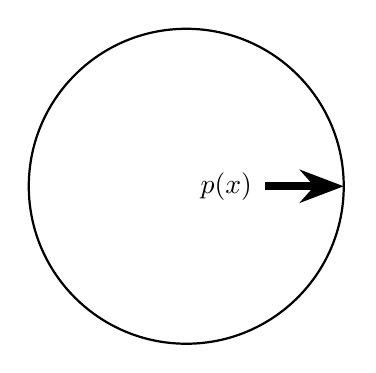
\begin{tikzpicture}[>=Stealth,scale=0.5, thick]
    \draw[line width=1 mm,->](2,0) node[left]{$p(x)$} -- (4,0);
    \draw [color=black] circle(4cm);
    \end{tikzpicture}
  \end{center}
\end{figure}

\begin{empheq}[box=\fboxTwo]{alignat*=3}
  &\mbox{\textbf{Surface tension for cylinder:}} &\hspace{0.5in} \Delta{}p=\frac{\sigma}{r}
\end{empheq}

\begin{empheq}[box=\fboxTwo]{alignat*=3}
  &\mbox{\textbf{Surface tension for sphere:}} &\hspace{0.5in} \Delta{}p=\frac{2\sigma}{r}
\end{empheq}

\begin{empheq}[box=\fboxTwo]{alignat*=3}
  &\mbox{\textbf{Young-Laplace equation:}} &\hspace{0.5in} \Delta{}p=\sigma\left(\frac{1}{r_{x}}+\frac{1}{r_{y}}\right)
\end{empheq}

Contact angle $\alpha$ is a property of the fluid, the material it is touching, and the third fluid it is in (like air).

\begin{empheq}[box=\fboxTwo]{alignat*=3}
  &\mbox{\textbf{Young's equation:}} &\hspace{0.5in} \cos\theta_{E}=\frac{\sigma_{sv}-\sigma_{sl}}{\sigma_{lv}}
\end{empheq}
where $s$, $l$, and $v$ are solid, liquid, and vapor, respectively, and $\theta_{E}$ is the equilibrium contact angle.

\chapter{Appendix}

\begin{empheq}[box=\fboxTwo]{alignat*=3}
  &\mbox{\textbf{Volume of sphere:}} &\hspace{0.5in} V=\frac{4}{3}\pi{}r^{3}
\end{empheq}

\begin{empheq}[box=\fboxTwo]{alignat*=3}
  &\mbox{\textbf{Surface area of sphere:}} &\hspace{0.5in} A=4\pi{}r^{2}
\end{empheq}

Power of fan or pump where $\dot{W}$ is the time derivative of work, aka power, and $\eta$ is the fan or pump efficiency.

\begin{equation*}
  \eta\dot{W}=\frac{1}{2}\rho{}v^{2}Q
\end{equation*}

Work of fluid with velocity $U$ applying force $F$

\begin{equation*}
  W_{\text{ext}}=FU
\end{equation*}

Power is

\begin{equation*}
  P=F_{\text{ext}}U
\end{equation*}

Work is
\begin{equation*}
  W=Q\Delta{}p
\end{equation*}

\section{Equation Summary Sheet}

\begin{empheq}[box=\fboxTwo]{alignat*=3}
  &\mbox{\textbf{Bernoulli's along streamline:}} &\hspace{0.5in} \frac{1}{2}\rho{}v_{s2}^{2}+p_{2}+\rho{}gz_{2}=\frac{1}{2}\rho{}v_{s1}^{2}+p_{1}+\rho{}gz_{1}
\end{empheq}

Reynolds transport theorem (form A)

\begin{equation*}
  \frac{d}{dt}\int_{CV(t)}\phi dV+\int_{CS}\phi (\underline{v}-\underline{v}_{c})\cdot\underline{n}dA=\frac{d}{dt}\int_{MV}\phi dV
\end{equation*}

Material Derivative

\begin{equation*}
  \rho\frac{D\underline{v}}{Dt}=\left(\frac{\partial\underline{v}}{\partial{}t}+\underline{v}\cdot\underline{\nabla}\underline{v}\right)
\end{equation*}

Navier Stokes Equation

\begin{equation*}
  \hspace{0.5in} \rho\frac{D\underline{v}}{Dt}=-\underline{\nabla}p+\mu\nabla^{2}\underline{v}+\rho\underline{g}
\end{equation*}

\begin{empheq}[box=\fboxTwo]{alignat*=3}
  &\mbox{\textbf{Incompressible Navier-Stokes}} \hspace{0.5in}& \rho\left(\frac{\partial\underline{v}}{\partial{}t}+\underline{v}\cdot\underline{\nabla}\underline{v}\right)=-\underline{\nabla}p+\mu\nabla^{2}\underline{v}+\rho\underline{g} \\
  & &\hspace{0.5in} \rho\frac{D\underline{v}}{Dt}=-\underline{\nabla}p+\underline{\nabla}\cdot\uuline{\sigma}+\rho\underline{g} \\
  & &\hspace{0.5in} \rho\frac{D\underline{v}}{Dt}=-\underline{\nabla}p+\mu\nabla^{2}\underline{v}+\rho\underline{g}
\end{empheq}

\begin{empheq}[box={\labelBox[Mass Conservation]}]{alignat*=3}
  &\mbox{\textbf{Form A:}} &\hspace{0.5in} \frac{d}{dt}\int_{CV(t)}\rho{}dV+\int_{CS(t)}\rho{}(\overline{v}-\overline{v}_{c})\cdot\overline{n}dA=0 \\[6pt]
  &\mbox{\textbf{Form B:}} &\hspace{0.5in} \int_{CV(t)}\frac{\partial\rho}{\partial{}t}dV+\int_{CS(t)}\rho{}v_{n}dA=0
\end{empheq}

\begin{equation*}
  v_{rn}=(\overline{v}-\overline{v}_{c})\cdot\overline{n}
\end{equation*}

$\overline{v}$ is the velocity across the control surface.

\begin{empheq}[box={\labelBox[Momentum Conservation]}]{alignat*=3}
  &\mbox{\textbf{Form A:}} &\hspace{0.5in} \frac{d}{dt}\int_{CV(t)}\rho\overline{v}dV+\int_{CS(t)}\rho\overline{v}(\overline{v}-\overline{v}_{c})\cdot\overline{n}dA=\overline{F}_{CV}(t) \\[6pt]
  &\mbox{\textbf{Form B:}} &\hspace{0.5in} \int_{CV(t)}\frac{\partial(\rho\overline{v})}{\partial{}t}dV+\int_{CS(t)}\rho\overline{v}v_{n}dA=\overline{F}_{CV}(t)
\end{empheq}

\begin{empheq}[box=\fboxTwo]{alignat*=3}
  &\mbox{\textbf{Vorticity:}} &\hspace{0.5in} \underline{\omega}=\underline{\nabla}\times\underline{v}
\end{empheq}

\begin{empheq}[box=\fboxTwo]{alignat*=3}
&\mbox{\textbf{Derivative of Error Function:}} &\hspace{0.5in} \frac{d}{dz}\text{erf}(z)=\frac{2}{\sqrt{\pi}}e^{-z^{2}}
\end{empheq}

\section{Stokes}

\subsection{From Stokes First Problem}

look at the dimensional analysis sheet and see that the time scale for the diffusion of viscous effects into the fluid are like
\begin{equation*}
  t_{c}\sim\frac{L^{2}}{\nu}
\end{equation*}
and we need to pick a characteristic length scale, which is usually the boundary layer thickness $\delta$.
This gives
\begin{equation*}
  t_{c}\sim\frac{\delta^{2}}{\nu}
\end{equation*}
Solving for $\delta$ we have
\begin{equation*}
  \delta\sim\sqrt{\nu{}t_{c}}
\end{equation*}
And we can approximate the shear stress as a linear velocity profile over the boundary layer
\begin{equation*}
  \tau_{w}\sim\frac{\mu{}U}{\delta}\sim\frac{\mu{}U}{\sqrt{\nu{}t}}
\end{equation*}
To find boundary layer growth, we have the characteristic time scale for convection
\begin{equation*}
  t_{c}=\frac{L}{U}
\end{equation*}
so Blasius boundary layer grows like
\begin{equation*}
  \delta\sim\sqrt{\frac{\nu{}L}{U}}
\end{equation*}
which is the solution for the growth over a flat plate.
But the boundary layer is usually really small compared to the radius of curvature of non-flat surfaces, so we can pretty much use this always.

\begin{empheq}[box={\labelBox[Lubrication Theory Equations: Cartesian]}]{alignat*=3}
  &\mbox{x-\textbf{momentum}} \hspace{0.5in}& \mu\frac{d^{2}v_{x}}{dy^{2}}-\frac{\partial{}p}{\partial{}x}+\rho{}g_{x}&=0 \\
  &\mbox{y-\textbf{momentum}} &\hspace{0.5in} \rho{}g_{y}-\frac{\partial{}p}{\partial{}y}&=0 \\
  &\mbox{\textbf{Continuity}} &\hspace{0.5in} \frac{\partial{}v_{x}}{\partial{}x}+\frac{\partial{}v_{y}}{\partial{}y}&=0
\end{empheq}

\subsection{Boundary Layer Equations in Cartesian Summary}

To summarize, the simplified equations are shown below.
\begin{empheq}[box={\labelBox[Boundary Layer Equations: Cartesian]}]{alignat*=3}
  &\mbox{x-\textbf{momentum}} \hspace{0.5in}& \rho\left(v_{x}\frac{\partial{}v_{x}}{\partial{}x}+v_{y}\frac{\partial{}v_{x}}{\partial{}y}\right)&=\mu\frac{\partial^{2}v_{x}}{\partial{}y^{2}}-\frac{\partial{}p}{\partial{}x} \\
  &\mbox{y-\textbf{momentum}} &\hspace{0.5in} \frac{\partial{}p}{\partial{}y}&=0 \\
  &\mbox{\textbf{Continuity}} &\hspace{0.5in} \frac{\partial{}v_{x}}{\partial{}x}+\frac{\partial{}v_{y}}{\partial{}y}&=0
\end{empheq}

We can see the shape that the boundary layer makes over a surface depending on the pressure gradient in the $x$-direction.
That is, at the surface we have $v_{x}=v_{y}=0$, so for $\frac{\partial{}p}{\partial{}x}<0$, $\frac{\partial{}p}{\partial{}x}=0$, and $\frac{\partial{}p}{\partial{}x}>0$ we can see the $\frac{\partial{}v_{x}}{\partial{}y}$, that is, the curvature of the velocity profile.

\begin{empheq}[box=\fboxTwo]{alignat*=3}
  &\mbox{\textbf{Displacement thickness}} \hspace{0.5in}& \delta^{*}&=\int_{0}^{\infty}\left(1-\frac{v_{x}(y)}{U_{\infty}}\right)dy \\
  &\mbox{\textbf{Momentum thickness}} \hspace{0.5in}& \theta&=\int_{0}^{\infty}\frac{v_{x}}{U_{\infty}}\left(1-\frac{v_{x}(y)}{U_{\infty}}\right)dy \\
  &\mbox{\textbf{Momentum Integral Equation}} \hspace{0.5in}& \frac{d}{dx}(U^{2}\theta)+\delta^{*}U\frac{dU}{dx}&=\frac{\tau_{0}}{\rho}
\end{empheq}

\begin{equation*}
  \delta\sim\sqrt{\nu{}t^{*}}
\end{equation*}

\begin{equation*}
  t^{*}=\frac{x}{U_{\infty}}
\end{equation*}

\begin{empheq}[box=\fboxTwo]{alignat*=3}
  &\mbox{\textbf{Young-Laplace equation:}} &\hspace{0.5in} \Delta{}p=\sigma\left(\frac{1}{r_{x}}+\frac{1}{r_{y}}\right)
\end{empheq}

\begin{empheq}[box=\fboxTwo]{alignat*=3}
  &\mbox{\textbf{Surface Tension Energy:}} &\hspace{0.5in} dE=\sigma{}dA \\
  & &\hspace{0.5in}  E_{\text{surf}}=\sigma{}A_{\text{surf}}
\end{empheq}

\section{What Formulas to use When}

If the question says, show that a given functional form satisfies some governing equation, rather than trying to derive the given functional form from some governing equation, instead pick a governing equation and plug the given functional form in just to check that it satisfies it.
Relating $u$ to $v$: think continuity!
When asked to compare gravity and surface tension forces, compare hydrostatic pressure of the whole column of fluid to the pressure due to surface tension as calculated from the Young-Laplace equation.

% TODO@dpwiese - Find general equations for Lubrication in cylindrical, and boundary layer in cylindrical

\section{Stuff to Remember for Quals}

\begin{equation*}
  \frac{\partial\rho}{\partial{}t}+\underline{\nabla}\cdot(\rho\underline{v})=0
\end{equation*}

\begin{equation*}
  \frac{\partial{}v_{x}}{\partial{}x}+\frac{\partial{}v_{y}}{\partial{}y}=0
\end{equation*}

\begin{equation*}
  \rho\left(\frac{\partial{}v_{x}}{\partial{}t}+v_{x}\frac{\partial{}v_{x}}{x}+v_{y}\frac{\partial{}v_{x}}{\partial{}y}+v_{z}\frac{\partial{}v_{x}}{\partial{}z}\right)=\mu\left[\frac{\partial^{2}v_{x}}{\partial{}x^{2}}+\frac{\partial^{2}v_{x}}{\partial{}y^{2}}+\frac{\partial^{2}v_{x}}{\partial{}z^{2}}\right]-\frac{\partial{}p}{\partial{}x}+\rho{}g_{x}
\end{equation*}

\begin{equation*}
  \frac{\partial\rho}{\partial{}t}+\frac{1}{r}(\rho{}rv_{r})+\frac{1}{r}\frac{\partial}{\partial\theta}(\rho{}v_{\theta})+\frac{\partial}{\partial{}z}(\rho{}v_{z})=0
\end{equation*}

\begin{equation*}
  \rho\left(\frac{\partial{}v_{z}}{\partial{}t}+v_{r}\frac{\partial{}v_{z}}{\partial{}r}+\frac{v_{\theta}}{r}\frac{\partial{}v_{z}}{\partial\theta}+v_{z}\frac{\partial{}v_{z}}{\partial{}z}\right)=\mu\left[\frac{1}{r}\frac{\partial}{\partial{}r}\left(r\frac{\partial{}v_{z}}{\partial{}r}\right)+\frac{1}{r^{2}}\frac{\partial^{2}v_{z}}{\partial\theta^{2}}+\frac{\partial^{2}v_{z}}{\partial{}z^{2}}\right]+\rho{}g_{z}-\frac{\partial{}p}{\partial{}z}
\end{equation*}

$\Delta{}p=\sigma\left(\frac{1}{r_{x}}+\frac{1}{r_{y}}\right)$

Boundary layer:
\begin{itemize}
  \setlength{\itemsep}{-4pt}
  \item{Start with Navier-Stokes equation in the $x-$ and $y$-direction, and conservation of mass}
  \item{Assume \textbf{steady, 2-D flow} and \textbf{neglect gravity} to simplify the Navier-Stokes equations}
  \item{Nondimensionalize to get the boundary layer equations}
  \begin{itemize}
    \item{Assume during the non-dimensionalization that $\textbf{Re}\mathbf{>>1}$}
    \item{$\left(\frac{L}{\delta}\right)^{2}\sim\text{Re}>>1$ so $\left(\frac{L}{\delta}\right)^{2}>>1$}
    \item{\textbf{Laminar}}
  \end{itemize}
\end{itemize}

\begin{equation*}
  \frac{d}{dt}\int_{CV(t)}\rho\overline{v}dV+\int_{CS(t)}\rho\overline{v}(\overline{v}-\overline{v}_{c})\cdot\overline{n}dA=\overline{F}_{CV}(t)
\end{equation*}


  \part{Dynamics and Modeling}
  \chapter{Linear and Angular Momentum Principles}

\section{Single Particle}

\begin{figure}[H]
  \begin{center}
    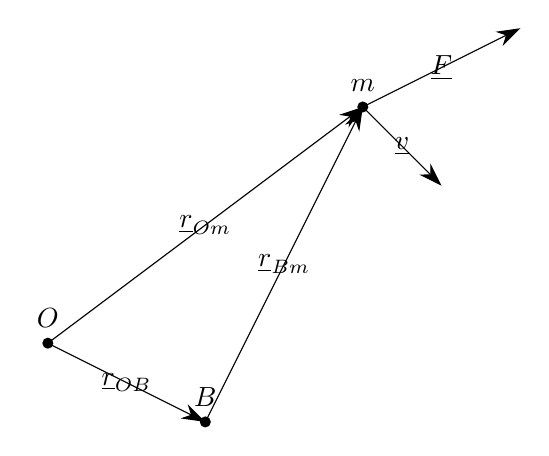
\begin{tikzpicture}[>={Stealth[width=2mm,length=3mm]}]
      \node[circle, fill=black, inner sep=0pt,minimum size=4pt, label=$m$] (m) at (0,0){};
      \node[circle, fill=black, inner sep=0pt,minimum size=4pt, label=$O$] (O) at (-4,-3){};
      \node[circle, fill=black, inner sep=0pt,minimum size=4pt, label=$B$] (B) at (-2,-4){};
      \draw [->] (-4,-3)--(0,0) node[pos=0.5] {$\underline{r}_{Om}$};
      \draw [->] (0,0)--(2,1) node[pos=0.5] {$\underline{F}$};
      \draw [->] (0,0)--(1,-1) node[pos=0.5] {$\underline{v}$};
      \draw [->] (-4,-3)--(-2,-4) node[pos=0.5] {$\underline{r}_{OB}$};
      \draw [->] (-2,-4)--(0,0) node[pos=0.5] {$\underline{r}_{Bm}$};
    \end{tikzpicture}
    \caption{\fontsize{10pt}{10pt}\selectfont\textbf{Point mass $m$ under action of force $\underline{f}$. Point $O$ is fixed in inertial space, and point $B$ is a general point, not necessarily fixed in inertial space.}}
  \end{center}
\end{figure}

\begin{empheq}[box=\fboxTwo]{alignat*=3}
  &\mbox{\textbf{Linear momentum:}}
  &\hspace{0.5in} \underline{p}=m\underline{v}
\end{empheq}

\begin{empheq}[box=\fboxTwo]{alignat*=3}
  &\mbox{\textbf{Linear momentum principle:}}
  &\hspace{0.5in} \underline{f}=\frac{d\underline{p}}{dt}
\end{empheq}

\begin{empheq}[box=\fboxTwo]{alignat*=3}
  &\mbox{\textbf{Torque about point} $O$:}
  &\hspace{0.5in} \tau_{O}=\underline{r}_{Om}\times\underline{f}
\end{empheq}

\begin{empheq}[box=\fboxTwo]{alignat*=3}
  &\mbox{\textbf{Moment of momentum about point} $O$:}
  &\hspace{0.5in} h_{O}=\underline{r}_{Om}\times\underline{p}
\end{empheq}

differentiate expression for $h_{O}$

\begin{equation*}
  \frac{d}{dt}\underline{h}_{O}=\frac{d}{dt}\underline{r}_{Om}\times\underline{p}+\underline{r}_{Om}\times\frac{d}{dt}\underline{p}
\end{equation*}

but

\begin{equation*}
  \frac{d}{dt}\underline{r}_{Om}=\underline{v}
\end{equation*}

and since $\underline{p}=m\underline{v}$ the cross product $\frac{d}{dt}\underline{r}_{Om}\times\underline{p}=0$ and so

\begin{equation*}
  \frac{d}{dt}\underline{h}_{O}=\underline{r}_{Om}\times\frac{d}{dt}\underline{p}
\end{equation*}

and substituting the linear momentum principle $\frac{d\underline{p}}{dt}=\underline{f}$ this gives

\begin{equation*}
  \frac{d}{dt}\underline{h}_{O}=\underline{r}_{Om}\times\underline{f}
\end{equation*}

But the right hand side is just the torque about point $O$, so we have

\begin{empheq}[box=\fboxTwo]{alignat*=3}
  &\mbox{\textbf{Angular momentum principle of particle about point} $O$:}
  &\hspace{0.5in} \underline{\tau}_{O}=\frac{d}{dt}\underline{h}_{O}
\end{empheq}

About a general point $B$ the torque and moment of momentum can be expressed as

\begin{equation*}
  \begin{split}
    \underline{\tau}_{B}&=\underline{r}_{Bm}\times\underline{f} \\
    \underline{h}_{B}&=\underline{r}_{Bm}\times\underline{p}
  \end{split}
\end{equation*}

Using $\underline{r}_{Bm}=\underline{r}_{Om}-\underline{r}_{OB}$ and substituting in we have

\begin{equation*}
  \begin{split}
    \underline{\tau}_{B}
    &=(\underline{r}_{Om}-\underline{r}_{OB})\times\underline{f} \\
    &=\underline{r}_{Om}\times\underline{f}-\underline{r}_{OB}\times\underline{f} \\
    &=\underline{\tau}_{O}-\underline{R}_{OB}\times\underline{f}
  \end{split}
\end{equation*}

\begin{empheq}[box=\fboxTwo]{alignat*=3}
  &\mbox{\textbf{Torque on particle about general point} $B$:}
  &\hspace{0.5in} \underline{\tau}_{B}=\underline{\tau}_{O}-\underline{r}_{OB}\times\underline{f}
\end{empheq}

and

\begin{equation*}
  \begin{split}
    \underline{h}_{B}&=(\underline{r}_{Om}-\underline{r}_{OB})\times\underline{p} \\
    &=\underline{r}_{Om}\times\underline{p}-\underline{r}_{OB}\times\underline{p} \\
    &=\underline{h}_{O}-\underline{r}_{OB}\times\underline{p}
  \end{split}
\end{equation*}

\begin{empheq}[box=\fboxTwo]{alignat*=3}
  &\mbox{\textbf{Moment of momentum of particle about gen.\ point} $B$:}
  &\hspace{0.5in} \underline{h}_{B}=\underline{h}_{O}-\underline{r}_{OB}\times\underline{p}
\end{empheq}

Evaluate the following

\begin{equation*}
  \begin{split}
    \frac{d}{dt}\underline{h}_{B}&=\frac{d}{dt}\underline{h}_{O}-\frac{d}{dt}\underline{r}_{OB}\times\underline{p}-\underline{r}_{OB}\times\frac{d}{dt}\underline{p} \\
    &=\underline{\tau}_{O}-\underline{v}_{B}\times\underline{p}-\underline{r}_{OB}\times\underline{f}
  \end{split}
\end{equation*}

From above we have $\underline{r}_{OB}\times\underline{f}=\underline{\tau}_{O}-\underline{\tau}_{B}$ and so we can write

\begin{equation*}
  \begin{split}
    \frac{d}{dt}\underline{h}_{B}&=\underline{\tau}_{O}-\underline{v}_{B}\times\underline{p}-\underline{\tau}_{O}+\underline{\tau}_{B} \\
    &=-\underline{v}_{B}\times\underline{p}+\underline{\tau}_{B}
  \end{split}
\end{equation*}

solving for $\underline{\tau}_{B}$ this gives

\begin{empheq}[box=\fboxTwo]{alignat*=3}
  &\mbox{\textbf{Angular momentum principle of particle about gen.\ point} $B$:}
  &\hspace{0.5in} \underline{\tau}_{B}=\frac{d}{dt}\underline{h}_{B}+\underline{v}_{B}\times\underline{p}
\end{empheq}

\section{General System (System of Particles)}

\begin{figure}[H]
  \begin{center}
    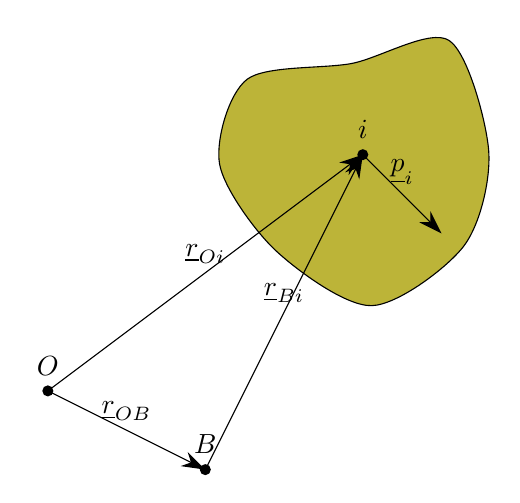
\begin{tikzpicture}[>={Stealth[width=2mm,length=3mm]}]
      \pgfmathsetseed{3}
      \draw [fill=yellow!70!black] plot [smooth cycle, samples=8,domain={1:8}] (\x*360/8+5*rnd:1.0cm+1.0cm*rnd) {};
      \node[circle, fill=black, inner sep=0pt,minimum size=4pt, label=$i$] (m) at (0,0){};
      \node[circle, fill=black, inner sep=0pt,minimum size=4pt, label=$O$] (O) at (-4,-3){};
      \node[circle, fill=black, inner sep=0pt,minimum size=4pt, label=$B$] (B) at (-2,-4){};
      \draw [->] (-4,-3)--(0,0) node[pos=0.5, above] {$\underline{r}_{Oi}$};
      \draw [->] (0,0)--(1,-1) node[pos=0.5, above] {$\underline{p}_{i}$};
      \draw [->] (-4,-3)--(-2,-4) node[pos=0.5, above] {$\underline{r}_{OB}$};
      \draw [->] (-2,-4)--(0,0) node[pos=0.5, above] {$\underline{r}_{Bi}$};
    \end{tikzpicture}
    \caption{\fontsize{10pt}{10pt}\selectfont\textbf{General system which is made up of many masses $m_{i}$, with total mass $M$. There are forces $\underline{f}_{i}$ acting on the $i$ particles. Point $O$ is fixed in inertial space, and point $B$ is a general point, not necessarily fixed in inertial space.}}
  \end{center}
\end{figure}

\begin{empheq}[box=\fboxTwo]{alignat*=3}
  &\mbox{\textbf{Linear momentum principle for general system:}}
  &\hspace{0.5in} \underline{F}^{\text{ext}}=\frac{d}{dt}\underline{P}
\end{empheq}

\begin{equation*}
  \underline{H}_{O}=[I]_{O}\omega
\end{equation*}

\begin{empheq}[box=\fboxTwo]{alignat*=3}
  &\mbox{\textbf{Angular momentum principle of general system about point} $O$:}
  &\hspace{0.5in} \underline{\tau}_{O}^{\text{ext}}=\frac{d}{dt}\underline{H}_{O}
\end{empheq}

\begin{empheq}[box=\fboxTwo]{alignat*=3}
  &\mbox{\textbf{Moment of momentum of general system about point} $B$:}
  &\hspace{0.5in} \underline{H}_{B}=\underline{H}_{O}+\underline{r}_{OB}\times\underline{P}
\end{empheq}

To find the angular momentum principle for general system about general point $B$, we take the derivative of above expression

% TODO@dpwiese - Check sign on above equation and this derivation

\begin{equation*}
  \begin{split}
    \frac{d}{dt}\underline{H}_{B}
    &=\frac{d}{dt}\underline{H}_{O}-\frac{d}{dt}\underline{r}_{OB}\times\underline{P}-\underline{r}_{OB}\times\frac{d}{dt}\underline{P} \\
    &=\underline{\tau}_{O}^{\text{ext}}-\underline{v}_{B}\times\underline{P}-\underline{r}_{OB}\times\underline{F}^{\text{ext}}
  \end{split}
\end{equation*}

but we have that

\begin{equation*}
  \begin{split}
    \underline{F}^{\text{ext}}=\sum_{i}\underline{f}_{i}^{\text{ext}}
  \end{split}
\end{equation*}
The angular momentum principle of a system about a general point is the following

\begin{empheq}[box=\fboxTwo]{alignat*=3}
  &\mbox{\textbf{Angular momentum principle about point} $B$:}
  &\hspace{0.5in} \underline{\tau}_{B}^{\text{ext}}=\frac{d}{dt}\underline{H}_{B}+\underline{v}_{B}\times\underline{P}
\end{empheq}

If we have another general point $A$ we can write

\begin{empheq}[box=\fboxTwo]{alignat*=3}
  &\mbox{\textbf{Moment of momentum of general system about point $B$:}}
  &\hspace{0.5in} \underline{H}_{B}=\underline{H}_{A}+\underline{r}_{BA}\times\underline{P}
\end{empheq}

\section{Kinematics of Rigid Bodies}

\begin{figure}[H]
  \begin{center}
    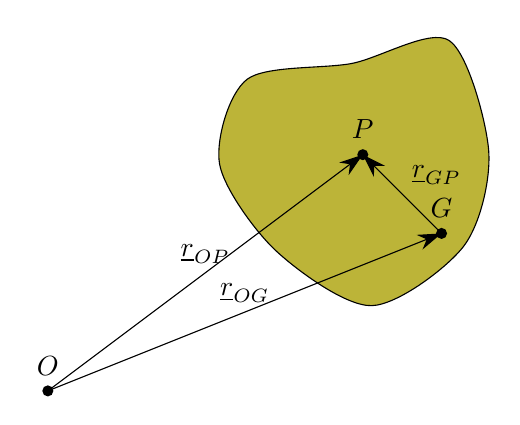
\begin{tikzpicture}[>={Stealth[width=2mm,length=3mm]}]
      \pgfmathsetseed{3}
      \draw [fill=yellow!70!black] plot [smooth cycle, samples=8,domain={1:8}] (\x*360/8+5*rnd:1.0cm+1.0cm*rnd) {};
      \node[circle, fill=black, inner sep=0pt,minimum size=4pt, label=$P$] (P) at (0,0){};
      \node[circle, fill=black, inner sep=0pt,minimum size=4pt, label=$O$] (O) at (-4,-3){};
      \node[circle, fill=black, inner sep=0pt,minimum size=4pt, label=$G$] (G) at (1,-1){};
      \draw [->] (-4,-3)--(0,0) node[pos=0.5, above] {$\underline{r}_{OP}$};
      \draw [->] (1,-1)--(0,0) node[pos=0.5, above right] {$\underline{r}_{GP}$};
      \draw [->] (-4,-3)--(1,-1) node[pos=0.5, above] {$\underline{r}_{OG}$};
    \end{tikzpicture}
    \caption{\fontsize{10pt}{10pt}\selectfont\textbf{Rigid Body. Point $O$ is fixed in inertial space, and point $B$ is a general point, not necessarily fixed in inertial space.}}
  \end{center}
\end{figure}

\begin{empheq}[box=\fboxTwo]{alignat*=3}
  &\mbox{\textbf{Velocity of point $P$ on rigid body relative to point $G$ on body}}
  &\hspace{0.5in} \underline{v}_{P}=\underline{v}_{G}+\underline{\omega}\times\underline{r}_{GP}
\end{empheq}

\subsection{Moment of Inertia}

\begin{empheq}[box=\fboxTwo]{alignat*=3}
  &\mbox{\textbf{Moment of inertia}}
  &\hspace{0.5in} \underline{H}_{B}=[I]_{B}\omega{}
\end{empheq}

To find principle axes

\begin{equation*}
  I_{\text{principal}}-\lambda I=0
\end{equation*}

\section{Impulse}

Take linear and angular momentum principle for a rigid body.
The linear and angular momentum principles for a system about a general point are given as follows.

\begin{empheq}[box=\fboxTwo]{alignat*=4}
  &\mbox{\textbf{Linear momentum principle for general system:}}
  &\hspace{0.5in} \underline{F}^{\text{ext}}&=\frac{d}{dt}\underline{P} \\[4pt]
  &\mbox{\textbf{Angular momentum principle about general point} $B$:}
  &\hspace{0.5in} \underline{\tau}_{B}^{\text{ext}}&=\frac{d}{dt}\underline{H}_{B}+\underline{v}_{B}\times\underline{P}
\end{empheq}

and separate them and integrate them over a short period of time

\begin{equation*}
  \begin{split}
    \int_{t=0^{-}}^{t=0^{+}}\underline{F}^{\text{ext}}dt&=\int_{\underline{P}(0^{-})}^{\underline{P}(0^{+})}d\underline{P} \\
    \int_{t=0^{-}}^{t=0^{+}}\underline{\tau}_{B}^{\text{ext}}dt&=\int_{\underline{H}_{B}(0^{-})}^{\underline{H}_{B}(0^{+})}d\underline{H}_{B}+\int_{t=0^{-}}^{t=0^{+}}\underline{v}_{B}\times\underline{P}dt
  \end{split}
\end{equation*}

\begin{equation*}
  \Delta\underline{P}=\int_{t=0^{-}}^{t=0^{+}}\underline{F}^{\text{ext}}dt
\end{equation*}

\chapter{Work and Energy Principles}

\begin{figure}[H]
  \begin{center}
    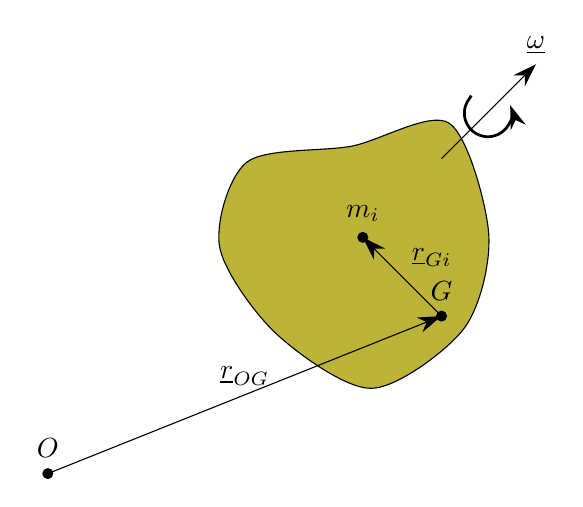
\begin{tikzpicture}[>={Stealth[width=2mm,length=3mm]}]
      \pgfmathsetseed{3}
      \draw [fill=yellow!70!black] plot [smooth cycle, samples=8,domain={1:8}] (\x*360/8+5*rnd:1.0cm+1.0cm*rnd) {};
      \node[circle, fill=black, inner sep=0pt,minimum size=4pt, label=$m_{i}$] (i) at (0,0){};
      \node[circle, fill=black, inner sep=0pt,minimum size=4pt, label=$O$] (O) at (-4,-3){};
      \node[circle, fill=black, inner sep=0pt,minimum size=4pt, label=$G$] (G) at (1,-1){};
      %\draw [->] (-4,-3)--(0,0) node[pos=0.5] {$\underline{r}_{Oi}$};
      \draw [->] (1,-1)--(0,0) node[pos=0.5, above right] {$\underline{r}_{Gi}$};
      \draw [->] (-4,-3)--(1,-1) node[pos=0.5, above] {$\underline{r}_{OG}$};
      \draw [->] (1,1)--(2.2,2.2) node[pos=0.5] (omega) {} node[pos=1.0, above] {$\underline{\omega}$};
      \draw [->,line width=1pt] (omega) ++ (138:3mm) --++ (60:-1pt) arc (-220:20:3mm) ;
    \end{tikzpicture}
    \caption{\fontsize{10pt}{10pt}\selectfont\textbf{Rigid Body. Point $O$ is fixed in inertial space, and point $B$ is a general point, not necessarily fixed in inertial space.}}
  \end{center}
\end{figure}

The kinetic energy of this rigid body is

\begin{equation*}
  T=\sum_{i}\frac{1}{2}m_{i}\underline{v}_{i}\cdot\underline{v}_{i}
\end{equation*}

In a rigid body $\underline{v}_{i}$ is given by

\begin{equation*}
  \underline{v}_{i}=\underline{v}_{G}+\underline{\omega}\times\underline{r}_{i}
\end{equation*}

Substituting this in we get the following expression

\begin{equation*}
  \begin{split}
    T&=\frac{1}{2}\left(\sum_{i}m_{i}\right)\underline{v}_{G}\cdot\underline{v}_{G}+\underline{v}_{G}\cdot\left(\underline{\omega}\times\sum_{i}m_{i}\underline{r}_{i}\right)+\frac{1}{2}\sum_{i}m_{i}(\underline{\omega}\times\underline{r}_{i})\cdot(\underline{\omega}\times\underline{r}_{i})
  \end{split}
\end{equation*}

The middle term drops out if $\underline{v}_{G}=0$ or if $G$ is at the center of mass of the body, allowing the kinetic energy to be written as

\begin{empheq}[box=\fboxTwo]{alignat*=3}
  &\mbox{\textbf{KE of rigid body about CM:}}
  &\hspace{0.5in} T=\frac{1}{2}M|\underline{v}_{G}|^{2}+\frac{1}{2}\sum_{i}m_{i}(\underline{\omega}\times\underline{r}_{i})\cdot(\underline{\omega}\times\underline{r}_{i})
\end{empheq}

\begin{empheq}[box=\fboxTwo]{alignat*=3}
  &\mbox{\textbf{KE of rigid body rotating about CM:}}
  &\hspace{0.5in} T=\frac{1}{2}Mv_{G}^{2}+\frac{1}{2}\left(I_{x}\omega_{x}^{2}+I_{y}\omega_{y}^{2}+I_{z}\omega_{z}^{2}\right)
\end{empheq}

\section{Finding Center of Mass and Moment of Inertia}

\begin{empheq}[box=\fboxTwo]{alignat*=3}
  &\mbox{\textbf{Finding CM:}}
  &\hspace{0.5in} x_{cm}=\frac{\sum_{i}A_{i}r_{i}}{\sum_{i}A_{i}}
\end{empheq}

\begin{empheq}[box=\fboxTwo]{alignat*=3}
  &\mbox{\textbf{Finding CM:}}
  &\hspace{0.5in} z_{cm}=\frac{\int_{m}zdm}{\int_{m}dm}
\end{empheq}

\begin{empheq}[box=\fboxTwo]{alignat*=3}
  &\mbox{\textbf{Finding CM:}}
  &\hspace{0.5in} z_{cm}=\frac{\int_{V}zdV}{\int_{V}dV}
\end{empheq}

\begin{empheq}[box=\fboxTwo]{alignat*=3}
  &\mbox{\textbf{Parallel axis theorem:}}
  &\hspace{0.5in} I_{B}=I_{0}+Mh^{2}
\end{empheq}

\begin{equation*}
  \begin{split}
    I_{x}&=\int_{m}(y^{2}+z^{2})dm \\
    I_{y}&=\int_{m}(x^{2}+z^{2})dm \\
    I_{z}&=\int_{m}(x^{2}+y^{2})dm
  \end{split}
\end{equation*}

constant density

\begin{equation*}
  \begin{split}
    I_{x}&=\rho\int_{V}(y^{2}+z^{2})dV \\
    I_{y}&=\rho\int_{V}(x^{2}+z^{2})dV \\
    I_{z}&=\rho\int_{V}(x^{2}+y^{2})dV
  \end{split}
\end{equation*}

\begin{example}[Cylinder]
  \begin{center}
    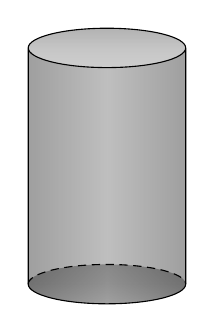
\begin{tikzpicture}[scale=0.5]
      \fill[top color=gray!50!black,bottom color=gray!10,middle color=gray,shading=axis,opacity=0.25] (0,0) circle (2cm and 0.5cm);
      \fill[left color=gray!50!black,right color=gray!50!black,middle color=gray!50,shading=axis,opacity=0.25] (2,0) -- (2,6) arc (360:180:2cm and 0.5cm) -- (-2,0) arc (180:360:2cm and 0.5cm);
      \fill[top color=gray!90!,bottom color=gray!2,middle color=gray!30,shading=axis,opacity=0.25] (0,6) circle (2cm and 0.5cm);
      \draw (-2,6) -- (-2,0) arc (180:360:2cm and 0.5cm) -- (2,6) ++ (-2,0) circle (2cm and 0.5cm);
      \draw [densely dashed] (-2,0) arc (180:0:2cm and 0.5cm);
    \end{tikzpicture}
  \end{center}
  \begin{center}
    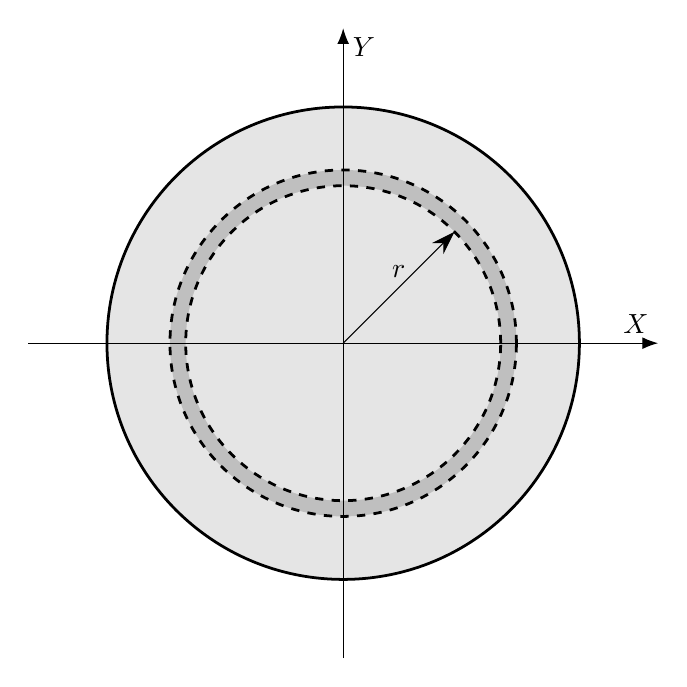
\begin{tikzpicture}[>={Stealth[width=2mm,length=3mm]}]
      \fill[color=gray!20] (0,0) circle(3);
      \fill[color=gray!50] (0,0) circle(2.2);
      \fill[color=gray!20] (0,0) circle(2.0);
      \draw [-{Latex[length=2mm]}] (-4,0) -- (4,0) node [above left]  {$X$};
      \draw [-{Latex[length=2mm]}] (0,-4) -- (0,4) node [below right] {$Y$};
      \draw [color=black, line width=1pt] (0,0) circle (3);
      \draw [color=black, line width=1pt,dashed] (0,0) circle (2);
      \draw [color=black, line width=1pt,dashed] (0,0) circle (2.2);
      \draw [->] (0,0)--(1.414,1.414) node[pos=0.5, above] {$r$};
    \end{tikzpicture}
  \end{center}
  By definition, the moment of inertia is

  \begin{equation*}
    I_{\text{cylinder},z}=\int_{V}\rho(x^{2}+y^{2})dV
  \end{equation*}
  The volume of a cylinder is given by

  \begin{equation*}
    V=\pi r^{2}L
  \end{equation*}
  A differential volume element is given by

  \begin{equation*}
    dV=2\pi rLdr
  \end{equation*}
  where $r^{2}=x^{2}+y^{2}$.
  Substituting this into the expression for moment of inertia

  \begin{equation*}
    \begin{split}
      I_{\text{cylinder}}
      &=\int_{0}^{R}\rho r^{2}2\pi rLdr \\
      &=2\pi L\rho\int_{0}^{R}r^{3}dr \\
    \end{split}
  \end{equation*}
  \begin{equation*}
    \begin{split}
      I_{\text{cylinder}}&=\frac{\pi L\rho R^{4}}{2}
    \end{split}
  \end{equation*}
  But, for a cylinder, $M=\rho V=\rho\phi R^{2}L$ giving

  \begin{empheq}[box=\roomyfbox]{equation*}
    I_{\text{cylinder}}=\frac{1}{2}MR^{2}
  \end{empheq}
\end{example}

\begin{example}[Rectangular Cube]
  \begin{center}
    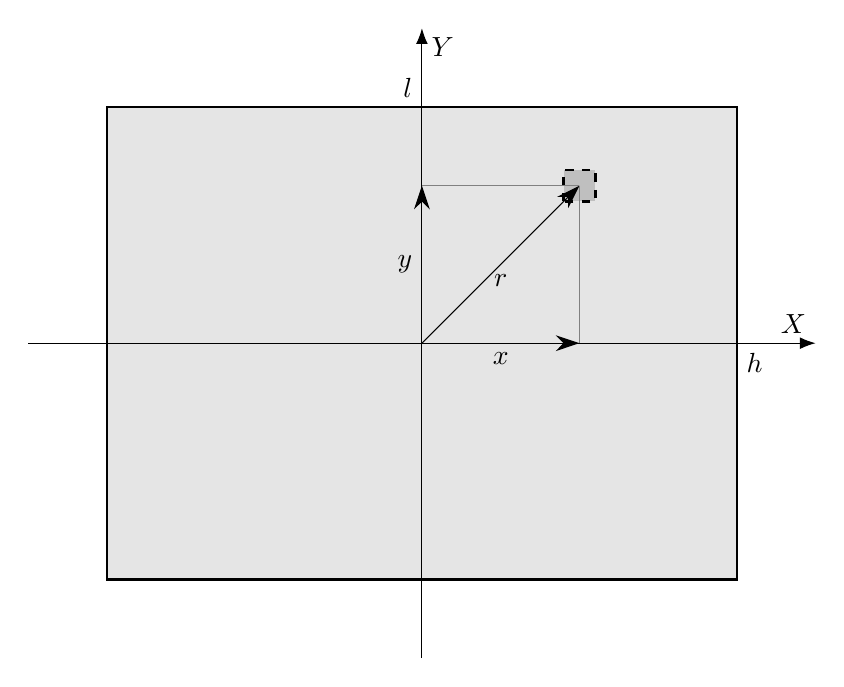
\begin{tikzpicture}[>={Stealth[width=2mm,length=3mm]}]
      \fill[color=gray!20] (0,0) (-4,-3)rectangle(4,3);
      \fill[color=gray!50] (2,2) (1.8,1.8)rectangle(2.2,2.2);
      \draw [color=black, line width=1pt] (0,0) (-4,-3)rectangle(4,3);
      \draw [color=black, line width=1pt,dashed] (2,2) (1.8,1.8)rectangle(2.2,2.2);
      \draw [-{Latex[length=2mm]}] (-5,0) -- (5,0) node [above left]  {$X$};
      \draw [-{Latex[length=2mm]}] (0,-4) -- (0,4) node [below right] {$Y$};
      \draw [->] (0,0)--(2,2) node[pos=0.5, below] {$r$};
      \draw [->] (0,0)--(2,0) node[pos=0.5, below] {$x$};
      \draw [->] (0,0)--(0,2) node[pos=0.5, left] {$y$};
      \draw [color=gray] (0,2)--(2,2);
      \draw [color=gray] (2,0)--(2,2);
      \draw (0,3) node [above left]  {$l$};
      \draw (4,0) node [below right]  {$h$};
    \end{tikzpicture}
  \end{center}
  This cube has depth $w$ into the page.
  $z$ axis is coming out of the page.
  By definition, the moment of inertia is

  \begin{equation*}
    I_{\text{cube},z}=\int_{V}\rho (x^{2}+y^{2})dV
  \end{equation*}
  The volume of a cube is given by

  \begin{equation*}
    V=wxy
  \end{equation*}
  A differential volume element is given by

  \begin{equation*}
    dV=wdxdy
  \end{equation*}
  Substituting this into the expression for moment of inertia

  \begin{equation*}
    I_{\text{cube},z}=\int_{-\frac{l}{2}}^{\frac{l}{2}}\int_{-\frac{h}{2}}^{\frac{h}{2}}\rho(x^{2}+y^{2})wdxdy
  \end{equation*}

  \begin{equation*}
    \begin{split}
      I_{\text{cube},z}&=\rho w\left[\int_{-\frac{h}{2}}^{\frac{h}{2}}(yx^{2}+\frac{y^{3}}{3})dx\right]_{y=-\frac{l}{2}}^{y=\frac{l}{2}} \\
      &=\rho w\int_{-\frac{h}{2}}^{\frac{h}{2}}\left(\frac{l}{2}x^{2}+\frac{l^{3}}{24}\right)-\left(-\frac{l}{2}x^{2}-\frac{l^{3}}{24}\right)dx \\
      &=\rho w\int_{-\frac{h}{2}}^{\frac{h}{2}}lx^{2}+\frac{l^{3}}{12}dx \\
      &=\rho w\left[\frac{l}{3}x^{3}+\frac{l^{3}}{12}x\right]_{x=-\frac{h}{2}}^{x=\frac{h}{2}} \\
      &=\rho w\left[\left(\frac{lh^{3}}{24}+\frac{hl^{3}}{24}\right)-\left(-\frac{lh^{3}}{24}-\frac{hl^{3}}{24}\right)\right]_{x=-\frac{h}{2}}^{x=\frac{h}{2}} \\
      &=\rho w\left(\frac{lh^{3}}{12}+\frac{hl^{3}}{12}\right) \\
      &=\rho wlh\left(\frac{h^{2}+l^{2}}{12}\right) \\
    \end{split}
  \end{equation*}

  \begin{empheq}[box=\roomyfbox]{equation*}
    I_{\text{cube},z}=m\frac{h^{2}+l^{2}}{12}
  \end{empheq}
\end{example}

\begin{example}[Sphere]
  \begin{equation*}
    V_{\text{sphere}}=\frac{4}{3}\pi r^{3}
  \end{equation*}
\end{example}

\begin{example}[Cone]
  \begin{center}
    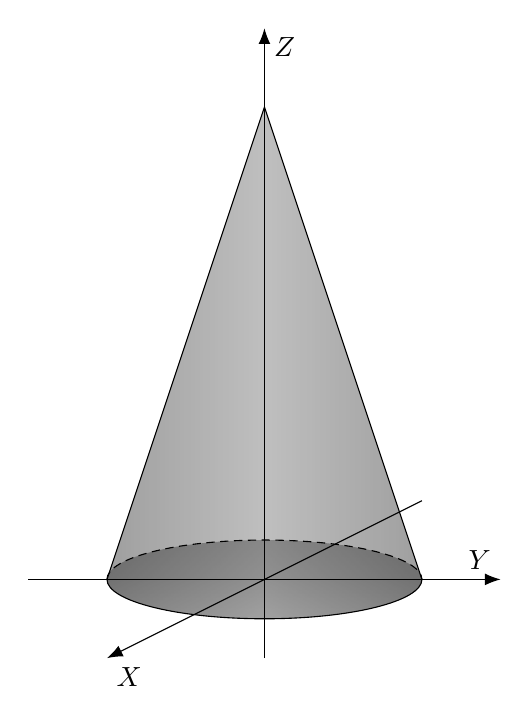
\begin{tikzpicture}[>={Latex[length=2mm]}]
      \fill[top color=gray!50!black,bottom color=gray!10,middle color=gray,shading=axis,opacity=0.25] (0,0) circle (2cm and 0.5cm);
      \fill[left color=gray!50!black,right color=gray!50!black,middle color=gray!50,shading=axis,opacity=0.25] (2,0) -- (0,6) -- (-2,0) arc (180:360:2cm and 0.5cm);
      \draw (-2,0) arc (180:360:2cm and 0.5cm) -- (0,6) -- cycle;
      \draw [densely dashed] (-2,0) arc (180:0:2cm and 0.5cm);
      \draw [->] (-3,0) -- (3,0) node [above left]  {$Y$};
      \draw [->] (0,-1) -- (0,7) node [below right] {$Z$};
      \draw [->] (2,1) -- (-2,-1) node [below right] {$X$};
    \end{tikzpicture}
  \end{center}
  Find the centroid.
  The cone is symmetric about the $z$ axis, so the centroid is along the $z$ axis, and we just need to find where.

  \begin{equation*}
    z_{cm}=\frac{\int_{m}zdm}{\int_{m}dm}
  \end{equation*}
  Since the cone has constant density we have that $dm=\rho dV$ and so this equation becomes the following, where the constant density is pulled out of the integral and cancels

  \begin{equation*}
    z_{cm}=\frac{\int_{V}zdV}{\int_{V}dV}
  \end{equation*}
  We integrate over this volume by using a stack of thin disks, and integrating from $z=0$ to $z=h$.
  Each disk has radius $r$.
  We find the formula for the disk radius with $z$ as

  \begin{equation*}
    r=R-\frac{R}{h}z
  \end{equation*}
  A differential volume element is given by

  \begin{equation*}
    \begin{split}
      dV&=\pi r^{2}dz \\
      &=\pi\left(R-\frac{R}{h}z\right)^{2}dz \\
      &=\pi R\left(1-\frac{1}{h}z\right)^{2}dz \\
      &=\pi R\left(1-\frac{2z}{h}+\frac{z^{2}}{h^{2}}\right)dz
    \end{split}
  \end{equation*}
  integrating
\end{example}

\begin{empheq}[box=\fboxTwo]{alignat*=3}
  &\mbox{\textbf{Cylinder radius $r$:}} &\hspace{0.5in} I_{\text{cylinder}}=\frac{1}{2}mr^{2} \\
  &\mbox{\textbf{Sphere radius $r$:}} &\hspace{0.5in} I_{\text{sphere}}=\frac{2}{5}mr^{2} \\
  &\mbox{\textbf{Rod length $L$ about end:}} &\hspace{0.5in} I_{\text{rod,end}}=\frac{1}{3}mL^{2} \\
  &\mbox{\textbf{Rod length $L$ about center:}} &\hspace{0.5in} I_{\text{rod,center}}=\frac{1}{12}mL^{2} \\
\end{empheq}

% % TODO@dpwiese - need this def here? Move it to preamble?
% \def\sc{1.6cm}

% \begin{tikzpicture} [x=\sc, y=\sc, line width = 1.5, >=angle 45 ]
%   % axes
%   \draw [line width=1, ->] (-.5,0) -- (2,0) node [right] {$x$};
%   \draw [line width=1, ->] (0,-.5) -- (0,2.3) node [above] {$y$};
%   % triangle
%   \draw (0,0) -- (1,0) -- (1,1.732) -- cycle;
%   % little element
%   \draw (.65,.5) coordinate (a) rectangle ++(.2,.2);
%   \draw [line width=1, gray] (0,0) -- (a) node [pos=.5,right, black] {$r$};
%   % ticks and labels
%   \draw [line width=1] (1,0) -- ++(0,-1ex) node [below] {$1$};
%   \draw [line width=1] (0,1.732) -- ++(-1ex,0) node [left] {$\sqrt3$};
%   \node at (1,.8) [right] {$r=\sec\theta$};
% \end{tikzpicture}

\chapter{Lagrange}

Holonomic system: the number of independent coordinates in the large is equal to the number of independent admissible variations.
Non-holonomic system is not holonomic.
Usually the number of admissible variations are less than the number of generalized coordinates.
Usually we can see nonholonomic systems by allowing the system to undergo large motions.
Remember example of coin rolling without slipping on table.

\begin{enumerate}
  \item{choose generalized coordinates in the large $\xi_{1},\dots,\xi_{n}$}
  \begin{itemize}
    \item{A complete set of coordinates should be able to exactly define the orientation of the system without ambiguity}
    \item{%
      An independent set of coordinates should not have any redundancy.
      In other words, none of the generalized coordinates should be able to be written in terms of the others.
      Should be the minimal amount of coordinates that can describe the orientation of the system
    }
  \end{itemize}
  \item{%
    Consider displacement about each of these coordinates one at a time, while holding all the others fixed.
    Calculate the incremental work $\delta W$ done by the external forces under the incremental displacement $\delta\xi_{j}$.
    Express this incremental work as $\delta W=\Xi_{j}\delta\xi_{j}$ to see what the generalized force is.
    Repeat this for each of the generalized coordinates.
  }
  \item{Find kinetic and potential energy $T$ and $V$ for the system.}
  \item{Make lagrangian $\mathscr{L}=T-V$}
  \item{Use the formula}
  \begin{equation*}
    \frac{d}{dt}\left(\frac{\partial\mathscr{L}}{\partial\dot{\xi}_{j}}\right)-\frac{\partial\mathscr{L}}{\partial\xi_{j}}=\Xi_{j}
  \end{equation*}
  That gives us the equations of motion
\end{enumerate}

\chapter{Problems}

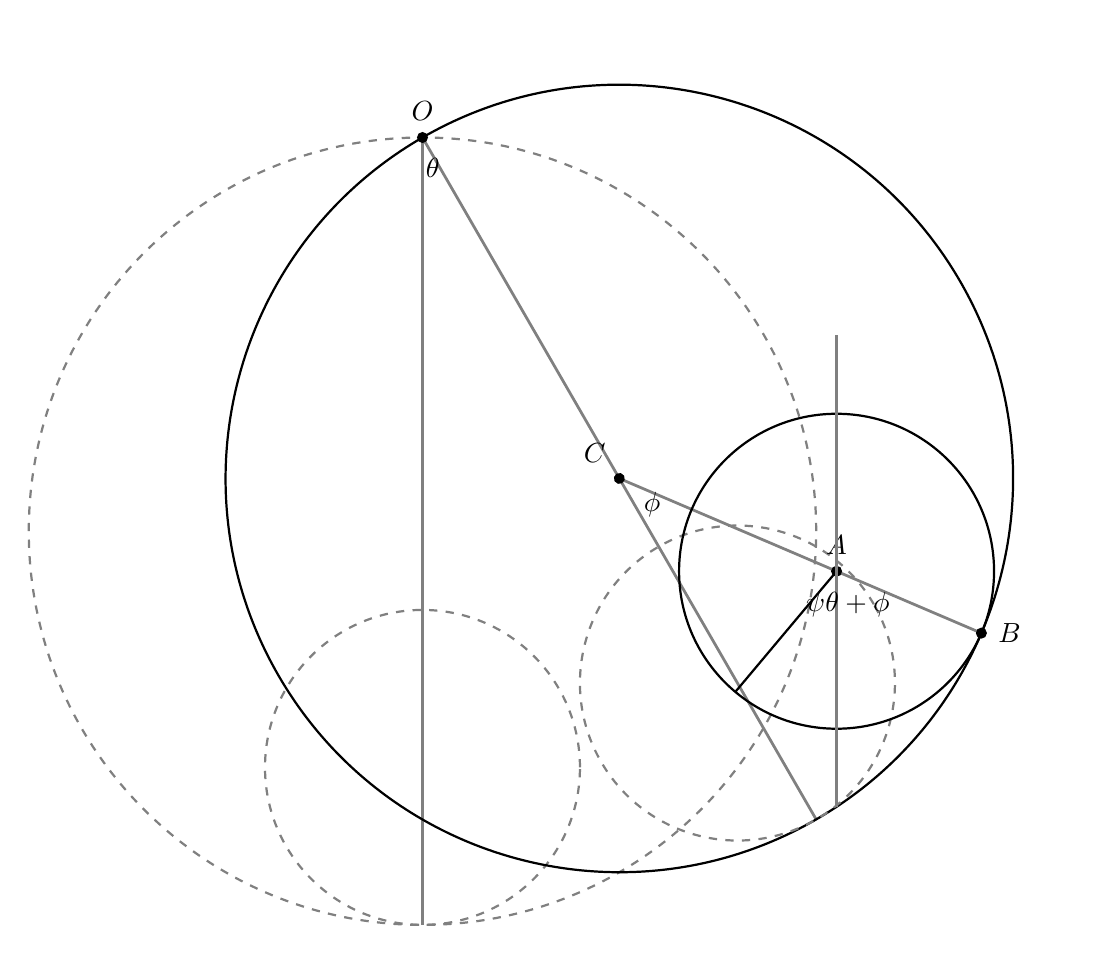
\begin{tikzpicture}[thick]
  %Original, undisplaced configuration
  \draw [color=gray, dashed] circle(5cm);
  \draw [color=gray, dashed] (0,-3) circle(2cm);
  \draw [color=gray, line width=1] (0,5) -- (0,-5);
  % Rotation about theta only, cylinder "glued" to ring
  \draw [color=gray, line width=1, rotate around={30:(0,5)}] (0,5) -- (0,-5) node[pos=0, name=O]{};
  \draw [rotate around={30:(0,5)}] circle(5cm);
  \draw [color=gray, dashed, rotate around={30:(0,5)}] (0,-3) circle(2cm);
  \draw [color=gray, line width=1, rotate around={30:(0,5)}] (0,0) -- (3,-4) node[pos=0.6, name=A]{} node[pos=1.0, name=B]{};
  \node  at (A) [draw,circle,minimum width=4cm] {};
  \node [circle, fill=black, inner sep=0pt,minimum size=4pt, label=$C$,rotate around={30:(0,5)}, name=C] (0,-5) {};
  \node at (O) [circle, fill=black, inner sep=0pt, minimum size=4pt, label=$O$] {};
  \node at (A) [circle, fill=black, inner sep=0pt, minimum size=4pt, label=$A$] {};
  \node at (B) [circle, fill=black, inner sep=0pt, minimum size=4pt, label=right:$B$] {};
  \node at (O) [label=below:$\theta$, anchor=west] {};
  \node [label=below:$\phi$, anchor=west, rotate around={30:(0,5)}] (0,-5){};
  \draw (A.center) --++ (230:2cm);
  \draw [color=gray] (A.center) --++ (0,3) --++ (0,-6);
  \node at (A.east) [label=below:$\theta+\phi$, anchor=west] {};
  \node at (A.west) [label=below:$\psi$, anchor=east] {};
\end{tikzpicture}

Looking at the arc lengths, and how the cylinder rolled inside the ring, with $\psi$ the absolute angular displacement of the cylinder, we have

\begin{equation*}
  \begin{split}
    (\psi+\theta+\phi)r&=\phi R \\
    \psi&=\frac{\phi(R-r)-\theta r}{r} \\
    \psi&=\phi\left(\frac{R}{r}-1\right)-\theta
  \end{split}
\end{equation*}

and so differentiating to get the angular velocity of the cylinder

\begin{equation*}
  \dot{\psi}=\dot{\phi}\left(\frac{R}{r}-1\right)-\dot{\theta}
\end{equation*}

But we can also find this relationship using first principles: equations for motions of rigid bodies.
Since there is no slip, we will find expressions for the velocity of the material point of the ring where it touches the cylinder (point $B$) and do the same for the material point of the cylinder where it touches the ring (again point $B$).
By equating these two expressions, we should be able to solve for $\dot{\psi}$ in terms of the two generalized coordinates $\theta$ and $\phi$ and their derivatives and constants.

\begin{equation*}
  \underline{v}_{B}\bigr|_{\text{ring}}=\underline{\omega}_{\text{ring}}\times\underline{r}_{OB}
\end{equation*}

\begin{empheq}[box=\roomyfbox]{equation*}
  \underline{\omega}_{\text{ring}}=\dot{\theta}\underline{\hat{e}}_{Z}
\end{empheq}

\begin{equation*}
  \underline{r}_{OB}=\underline{r}_{OC}+\underline{r}_{CB}
\end{equation*}

\begin{equation*}
  \underline{r}_{OC}=R\sin\theta\underline{\hat{e}}_{X}-R\cos\theta\underline{\hat{e}}_{Y}
\end{equation*}

\begin{equation*}
  \underline{r}_{CB}=R\sin(\theta+\phi)\underline{\hat{e}}_{X}-R\cos(\theta+\phi)\underline{\hat{e}}_{Y}
\end{equation*}

\begin{equation*}
  \underline{v}_{B}\bigr|_{\text{ring}}=\dot{\theta}R(\sin\theta+\sin(\theta+\phi))\underline{\hat{e}}_{Y}+\dot{\theta}R(\cos\theta+\cos(\theta+\phi))\underline{\hat{e}}_{X}
\end{equation*}

\begin{equation*}
  \underline{v}_{B}\bigr|_{\text{disk}}=\underline{v}_{A}+\underline{\omega}_{\text{disk}}\times\underline{r}_{AB}
\end{equation*}

\begin{equation*}
  \underline{v}_{A}=\underline{v}_{C}+(\dot{\theta}+\dot{\phi})\underline{\hat{e}}_{Z}\times\underline{r}_{OC}
\end{equation*}

\begin{equation*}
  \underline{v}_{C}=\dot{\theta}\underline{\hat{e}}_{Z}\times\underline{r}_{OC}
\end{equation*}

\begin{empheq}[box=\roomyfbox]{equation*}
  \underline{v}_{C}=\dot{\theta}R\sin\theta\underline{\hat{e}}_{Y}+\dot{\theta}R\cos\theta\underline{\hat{e}}_{X}
\end{empheq}

\begin{equation*}
  \underline{r}_{CA}=(R-r)\sin(\theta+\phi)\underline{\hat{e}}_{X}-(R-r)\cos(\theta+\phi)\underline{\hat{e}}_{Y}
\end{equation*}

\begin{equation*}
  \underline{v}_{A}=\dot{\theta}R\cos\theta\underline{\hat{e}}_{X}+\dot{\theta}R\sin\theta\underline{\hat{e}}_{Y}+(\dot{\theta}+\dot{\phi})(R-r)\sin(\theta+\phi)\underline{\hat{e}}_{Y}+(\dot{\theta}+\dot{\phi})(R-r)\cos(\theta+\phi)\underline{\hat{e}}_{X}
\end{equation*}

\begin{empheq}[box=\roomyfbox]{equation*}
  \underline{v}_{A}=\bigr(\dot{\theta}R\cos\theta+(\dot{\theta}+\dot{\phi})(R-r)\cos(\theta+\phi)\bigr)\underline{\hat{e}}_{X}+\bigr(\dot{\theta}R\sin\theta+(\dot{\theta}+\dot{\phi})(R-r)\sin(\theta+\phi)\bigr)\underline{\hat{e}}_{Y}
\end{empheq}

\begin{equation*}
  \underline{v}_{B}\bigr|_{\text{disk}}=\underline{v}_{A}-\omega_{\text{disk}}\underline{\hat{e}}_{Z}\times(r\sin(\theta+\phi)\underline{\hat{e}}_{X}-r\cos(\theta+\phi)\underline{\hat{e}}_{Y})
\end{equation*}
Equating the two velocities of disk and ring, and separating into $X$ and $Y$ components we have

\begin{equation*}
  \begin{split}
    \dot{\theta}R\cos\theta+\dot{\theta}R\cos(\theta+\phi)&=\dot{\theta}R\cos\theta+(\dot{\theta}+\dot{\phi})(R-r)\cos(\theta+\phi)-\omega_{\text{disk}}r\cos(\theta+\phi) \\
    \dot{\theta}R(\sin\theta+\sin(\theta+\phi))&=\dot{\theta}R\sin\theta+(\dot{\theta}+\dot{\phi})(R-r)\sin(\theta+\phi)=\omega_{\text{disk}}r\sin(\theta+\phi)
  \end{split}
\end{equation*}
and both these equations simplify to

\begin{equation*}
  \dot{\theta}R=(\dot{\theta}+\dot{\phi})(R-r)-\omega_{\text{disk}}r
\end{equation*}
giving

\begin{equation*}
  \omega_{\text{disk}}=\dot{\phi}\left(\frac{R}{r}-1\right)-\dot{\theta}
\end{equation*}

\begin{empheq}[box=\roomyfbox]{equation*}
  \underline{\omega}_{\text{disk}}=\left\{\dot{\phi}\left(\frac{R}{r}-1\right)-\dot{\theta}\right\}\underline{\hat{e}}_{Z}
\end{empheq}
Now start doing Lagrangian stuff.
Start by writing an expression for the kinetic energy $T$ and potential energy $V$.

\begin{equation*}
  I_{\text{ring}}=MR^{2}
\end{equation*}

\begin{equation*}
  I_{\text{disk}}=\frac{1}{2}mr^{2}
\end{equation*}

\begin{empheq}[box=\roomyfbox]{equation*}
  V=-MgR\cos\theta-mg(R\cos\theta+\cos(\theta+\phi)(R-r))
\end{empheq}

\begin{equation*}
  T=\frac{1}{2}M\underline{v}_{C}\cdot\underline{v}_{C}+\frac{1}{2}I_{\text{ring}}\omega_{\text{ring}}^{2}+\frac{1}{2}m\underline{v}_{A}\cdot\underline{v}_{A}+\frac{1}{2}I_{\text{disk}}\omega_{\text{disk}}^{2}
\end{equation*}

\begin{equation*}
  \begin{split}
    \underline{v}_{C}\cdot\underline{v}_{C}
    &=(\dot{\theta}R\sin\theta)^{2}+(\dot{\theta}R\cos\theta)^{2} \\
    &=\dot{\theta}^{2}R^{2}
  \end{split}
\end{equation*}

\begin{equation*}
  \omega_{\text{ring}}^{2}=\dot{\theta}^{2}
\end{equation*}

\begin{equation*}
  \begin{split}
    \underline{v}_{A}\cdot\underline{v}_{A}
    &= (\dot{\theta}R\cos\theta+(\dot{\theta}+\dot{\phi})(R-r)\cos(\theta+\phi))^{2} \\
    &+ (\dot{\theta}R\sin\theta+(\dot{\theta}+\dot{\phi})(R-r)\sin(\theta+\phi))^{2}
  \end{split}
\end{equation*}

\begin{equation*}
  \begin{split}
    \underline{v}_{A}\cdot\underline{v}_{A}
    &= \dot{\theta}^{2}R^{2}\cos^{2}\theta+2\dot{\theta}R\cos\theta(\dot{\theta} \\
    &+ \dot{\phi})(R-r)\cos(\theta+\phi)+(\dot{\theta}+\dot{\phi})^{2}(R-r)^{2}\cos^{2}(\theta+\phi) \\
    &+ \dot{\theta}^{2}R^{2}\sin^{2}\theta+2\dot{\theta}R\sin\theta(\dot{\theta}+\dot{\phi})(R-r)\sin(\theta+\phi) \\
    &+ (\dot{\theta}+\dot{\phi})^{2}(R-r)^{2}\sin^{2}(\theta+\phi)
  \end{split}
\end{equation*}

\begin{equation*}
  \begin{split}
    \underline{v}_{A}\cdot\underline{v}_{A}
    &= \dot{\theta}^{2}R^{2}+(\dot{\theta}+\dot{\phi})^{2}(R-r)^{2} \\
    &+ 2\dot{\theta}R\cos\theta(\dot{\theta}+\dot{\phi})(R-r)\cos(\theta+\phi) \\
    &+ 2\dot{\theta}R\sin\theta(\dot{\theta}+\dot{\phi})(R-r)\sin(\theta+\phi)
  \end{split}
\end{equation*}

\begin{equation*}
  \begin{split}
    \underline{v}_{A}\cdot\underline{v}_{A}
    &= \dot{\theta}^{2}R^{2}+(\dot{\theta}+\dot{\phi})^{2}(R-r)^{2} \\
    &+ 2\dot{\theta}R(\dot{\theta}+\dot{\phi})(R-r)\bigr(\cos\theta\cos(\theta+\phi)+\sin\theta\sin(\theta+\phi)\bigr)
  \end{split}
\end{equation*}

\begin{equation*}
  \cos\theta\cos(\theta+\phi)+\sin\theta+\sin(\theta+\phi)=\cos(-\phi)=\cos\phi
\end{equation*}

\begin{equation*}
  \underline{v}_{A}\cdot\underline{v}_{A}
  = \dot{\theta}^{2}R^{2}+(\dot{\theta}+\dot{\phi})^{2}(R-r)^{2}+2\dot{\theta}R(\dot{\theta}+\dot{\phi})(R-r)\cos\phi
\end{equation*}

\begin{equation*}
  \omega_{\text{disk}}^{2}=\left\{\dot{\phi}\left(\frac{R}{r}-1\right)-\dot{\theta}\right\}^{2}
\end{equation*}

\begin{equation*}
  \begin{split}
    T
    &= \frac{1}{2}M\dot{\theta}^{2}R^{2}+\frac{1}{2}MR^{2}\dot{\theta}^{2} \\
    &+ \frac{1}{2}m\left(\dot{\theta}^{2}R^{2}+(\dot{\theta}+\dot{\phi})^{2}(R-r)^{2} + 2\dot{\theta}R(\dot{\theta}+\dot{\phi})(R-r)\cos\phi\right) \\
    &+ \frac{1}{4}mr^{2}\left\{\dot{\phi}\left(\frac{R}{r}-1\right)-\dot{\theta}\right\}^{2}
  \end{split}
\end{equation*}

\begin{empheq}{alignat*=3}
  T
  &= M\dot{\theta}^{2}R^{2} \\
  &\qquad+\frac{1}{2}m\Bigl(\dot{\theta}^{2}R^{2}
  + (\dot{\theta}+\dot{\phi})^{2}(R-r)^{2}+2\dot{\theta}R(\dot{\theta}
  + \dot{\phi})(R-r)\cos\phi\Bigr) \\
  &\qquad+\frac{1}{4}mr^{2}\left\{\dot{\phi}\left(\frac{R}{r}-1\right)-\dot{\theta}\right\}^{2}
\end{empheq}

\begin{empheq}[box=\roomyfbox]{alignat*=3}
  T
  &= M\dot{\theta}^{2}R^{2}+\frac{1}{2}m\dot{\theta}^{2}R^{2} \\
  &\qquad+ \frac{1}{2}m(\dot{\theta}^{2}+2\dot{\phi}\dot{\theta}+\dot{\phi}^{2})(R-r)^{2} \\
  &\qquad+ mR(\dot{\theta}^{2}+\dot{\phi}\dot{\theta})(R-r)\cos\phi{} \\
  &\qquad+ \frac{1}{4}mr^{2}\left\{\dot{\phi}\left(\frac{R}{r}-1\right)-\dot{\theta}\right\}^{2}
\end{empheq}

\begin{equation*}
  V=-MgR\cos\theta-mg(R\cos\theta+\cos(\theta+\phi)(R-r))
\end{equation*}

\begin{equation*}
  \mathscr{L}=T-V
\end{equation*}

\begin{equation*}
  \begin{split}
    \frac{\partial\mathscr{L}}{\partial\dot{\theta}}
    &= 2M\dot{\theta}R^{2}+m\dot{\theta}R^{2}+m(\dot{\theta}+\dot{\phi})(R-r)^{2} \\
    &+ mR(2\dot{\theta}+\dot{\phi})(R-r)\cos\phi+\frac{1}{2}mr^{2}\left\{\dot{\phi}\left(\frac{R}{r}-1\right)-\dot{\theta}\right\}
  \end{split}
\end{equation*}

\begin{equation*}
  \frac{\partial\mathscr{L}}{\partial\theta}=MgR\sin\theta+mgR\sin\theta+mg\sin(\theta+\phi)(R-r)
\end{equation*}

\begin{equation*}
  \frac{\partial\mathscr{L}}{\partial\dot{\phi}}=m(\dot{\theta}+\dot{\phi})(R-r)^{2}+mR\dot{\theta}(R-r)\cos\phi+\frac{1}{2}mr^{2}\left\{\dot{\phi}\left(\frac{R}{r}-1\right)-\dot{\theta}\right\}\left(\frac{R}{r}-1\right)
\end{equation*}

\begin{equation*}
  \frac{\partial\mathscr{L}}{\partial\phi}=
\end{equation*}

\section{Wave Equation on String}

This page gives an outline of the general procedure to derive the equation of motion, propose a general solution, and solve for constants using boundary and initial conditions (here we assume the boundary conditions are both ends fixed, and zero initial conditions just to get the mode shapes and natural frequencies.)

\textbf{Physical assumptions:} \textit{homogenous string $\rho A=\text{constant}$, the string is perfectly elastic (no resistance to bending), the tension is way more than gravity, and string only vibrates perfectly up and down.}

\begin{enumerate}
  \setlength{\itemsep}{0pt}
  \item{\textbf{Derive governing equation}}
  \begin{enumerate}
    \setlength{\itemsep}{0pt}
    \item{Momentum in $x$-direction gives $T(x)$ is constant}
    \item{Do momentum in the $y$-direction}
    \item{Use small angles: $\sin(\alpha+\frac{\partial\alpha}{\partial{}x}dx)=\alpha+\frac{\partial\alpha}{\partial{}x}dx$ and $\tan(\alpha)=\alpha$}
  \end{enumerate}
  The governing equation is $\boxed{T\frac{\partial^{2}y}{\partial{}x^{2}}=\rho A\frac{\partial^{2}y}{\partial{}t^{2}}}$
  \item{\textbf{Propose a general separable solution} $\boxed{y(x,t)=a(x)f(t)}$}
  \begin{enumerate}
    \setlength{\itemsep}{0pt}
    \item{Rearrange the governing equation as $C^{2}\frac{\partial^{2}y}{\partial{}x^{2}}=\frac{\partial^{2}y}{\partial{}t^{2}}$ and propose $f(t)=Ae^{i\omega_{n}t}$ giving $y(x,t)=a(x)Ae^{i\omega_{n}t}$ and plug in}
    \item{The governing equation becomes $C^{2}\frac{\partial^{2}a}{\partial{}x^{2}}+\omega_{n}^{2}a(x)=0$}
    \item{Propose $a(x)=Be^{i\lambda x}$ and get $\omega_{n}=C\lambda$}
    \item{The total solution is then $\boxed{y(x,t)=Be^{i\frac{\omega_{n}}{C} x}Ae^{i\omega_{n}t}}$ which can be decomposed into sine and cosine as $y(x,t)=(B_{1}\sin(\lambda x)+B_{2}\cos(\lambda x))(A_{1}\sin(\omega_{n}t)+A_{2}\cos(\omega_{n}t))$}
  \end{enumerate}
  \item{\textbf{Apply boundary and initial conditions} to get the constants}
  \begin{enumerate}
    \setlength{\itemsep}{0pt}
    \item{%
      Apply boundary conditions $y(x=0,t)=y(x=L,t)=0$ gives $B_{2}=0$ and $B_{1}\sin(\frac{\omega_{n}}{C}L)=0$ so $\frac{\omega_{n}}{C}L=n\pi$ where $n=1,2,3\dots$.
      So $\omega_{n}=\frac{Cn\pi}{L}$.
      The solution becomes $y(x,t)=B_{1}\sin(\frac{\omega_{n}}{C}x)(A_{1}\sin(\omega_{n}t)+A_{2}\cos(\omega_{n}t))$
    }
    \item{Apply initial conditions $y(x,t=0)=0$ gives $A_{2}=0$ reducing solution to $y(x,t)=B_{1}\sin(\frac{\omega_{n}}{C}x) A_{1}\sin(\omega_{n}t)$ or by combining the constants \newline $\boxed{y(x,t)=C_{n}\sin(\frac{\omega_{n}}{C}x)\sin(\omega_{n}t)}$}
  \end{enumerate}
  \item{Now we have the governing equation, now we see if it is \textbf{self-adjoint} if it satisfies the following conditions}
  \begin{enumerate}[(i)]
    \setlength{\itemsep}{0pt}
    \item{$\int u\rho Avdx=\int v\rho Audx$}
    \item{$\int v\left(-T\frac{\partial^{2}}{\partial{}x^{2}}\right)udx=\int u\left(-T\frac{\partial^{2}}{\partial{}x^{2}}\right)vdx$}
  \end{enumerate}
  The first condition is satisfied automatically, since $u$ and $v$ (in our case $a(x)$ and $f(t)$ commute.)
  We show that the second condition holds by doing integration by parts twice.
  \begin{equation*}
    \begin{split}
      &\int_{0}^{L}a_{i}\left(-T\frac{\partial^{2}}{\partial{}x^{2}}\right)a_{j}dx \\
      &= a_{i}\left(-T\frac{\partial}{\partial{}x}(a_{j})\right)\biggr|_{0}^{L}+\int_{0}^{L}T\frac{\partial}{\partial{}x}(a_{j})\frac{da_{i}}{dx}dx
    \end{split}
  \end{equation*}
  one more integration by parts
  \begin{equation*}
    \begin{split}
      &\int_{0}^{L}a_{i}\left(-T\frac{\partial^{2}}{\partial{}x^{2}}\right)a_{j}dx \\
      &=a_{i}\left(-T\frac{\partial}{\partial{}x}(a_{j})\right)\biggr|_{0}^{L}-\left(\frac{da_{i}}{dx}(-Ta_{j})\right)\biggr|_{0}^{L}+\int_{0}^{L}a_{j}\left(-T\frac{\partial^{2}}{\partial{}x^{2}}(a_{i})\right)dx
      \end{split}
  \end{equation*}
  and since we evaluate the first two terms on the right hand side at $x=0$ and $x=L$, the boundary conditions dictate that $a_{i}=a_{j}=0$ here, thus proving the system is \textbf{self-adjoint}.
  \textit{Self-adjointness depends on the boundary conditions.}
  \item{Now we use the self adjoint property to show that the modes are \textbf{orthogonal}, where $a_{j}$ and $a_{i}$ are orthogonal functions if they satisfy}
  \begin{equation*}
    \int_{0}^{L}a_{j}a_{i}dx=0
  \end{equation*}
\end{enumerate}

  \chapter{Aircraft Equations of Motion}

\section{Introduction}

The equations of rigid body motion are expanded and expressed in state space form.
The expression of the equations in this form assumes the Earth is flat, and inertially fixed.
The atmosphere is stationary with respect to the Earth.

\begin{itemize}
  \item{Show linear equations represented in stability axes \dots}
  \item{Show Taylor series expansion}
  \item{%
    Stability derivative has dimensions.
    Stability coefficient does not\ (Nelson pg 109).
  }
  \item{Express stability derivatives in terms of stability coefficients}
  \item{How to know before linearization that longitudinal and lateral equations can be decoupled?}
\end{itemize}

\subsection{Notation}

I use $R$ for rotation matrix, and $T$ for the transformation matrix from body axes to Euler axes.
Etkin uses $L$ for rotation matrices, and $\boldsymbol{R}$ for the transformation matrix from body axes to Euler axes.
Bilimoria and Schmidt use $[T]$ for rotation matrices and $[L]$ for the transformation matrix from body axes to Euler axes.
Some of the standard notation describing the expression of vectors in various reference frames is outlined below.

\begin{itemize}
  \item{%
    $F_{a}$ denotes reference frame $a$ in Etkin.
    I will use lower-case $f_{a}$ to denote reference frame $a$.
  }
  \item{$v_{a}$ describes vector $v$ of a point along axes of reference frame $a$, when the referred point is obvious.}
  \item{$v_{0}$ indicates the velocity of point $0$.}
  \item{$v_{0_{a}}$ indicates the velocity of point $0$ along the axes of reference frame $a$.}
  \item{%
    SUPERSCRIPT BASICALLY MEANS RELATIVE TO.\@
    Bilimoria and Schmidt use $|^{\cdot}$ instead of just a superscript, and often when there is no superscript, it is implied that it is actually relative to body axes.
  }
  \item{%
    A superscript indicates motion relative to a certain reference frame.
    $v^{a}$ is the velocity of a point relative to frame $f_{a}$, when the referred point is obvious.
  }
  \item{The notation ${v_{b}}^{a}$ gives the velocity of a point relative to reference frame $f_{a}$ described along the axes of $f_{b}$.}
  \item{To be clear, when the point of interest is not obvious, or there are multiple points, the notation ${v_{0_{b}}}^{a}$ would describe the velocity of point $0$ relative to reference frame $f_{a}$, described along the axes of $f_{b}$.}
  \item{%
    $\omega$ is typically reserved to describe the angular velocity of a reference frame relative to inertial axes $f_{I}$.
    Making use of the notation above, $\omega^{E}$ represents the angular velocity of reference frame $f_{E}$ relative to $f_{I}$\ (pretty sure this is from Etkin).
    Bilimoria and Schmidt: $\omega_{1,2}$ is the angular velocity of reference frame 1 relative to reference frame 2.
    This implies vector is expressed in the coordinates of reference frame 2?
  }
  \item{In Bilimoria and Schmidt $V_{I}$ is the inertial velocity of the vehicle}
  \begin{itemize}
    \item{$I$ is inertial frame}
    \item{$EC$ is Earth-centered, Earth-fixed frame}
    \item{$E$ is Earth-surface frame}
    \item{$V$ is vehicle carrying frame}
    \item{$V$ is vehicle-carried frame}
    \item{$A$ is atmosphere-fixed frame}
    \item{$W$ is air-trajectory frame (wind axes)}
    \item{$B$ is body-fixed frame (body axes)}
    \item{$S$ stability axes (special set of body axes)}
  \end{itemize}
  \item{The transformation $R_{ab}$ describes a vector transformation from being expressed in reference frame $b$ to being expressed in reference frame $a$.}
  \item{Typically capital letter denotes vector quantity}
\end{itemize}

\section{Equations of Motion}

In this problem, the rigid body equations of motion shown in Equations (\ref{force_eqn}-\ref{location_eqn}) below were expanded and expressed in a state space representation.
% TODO@dpwiese - Fix: velocity of which frame, relative to what other frame, expressed along the axes of which frame?
See Steven's and Lewis page 44 for moment equation derivation.
Poisson orientation equations page 28, and list of different kinematic equations page 46.

\begin{itemize}
  \item{%
    Flat earth, this defined the reference frames.
    A constant velocity in the flat earth does not lead to moments, but on a spherical earth it does.
  }
  \item{The aircraft is a rigid body thus has no rotating terms due to rotating turbo machinery}
\end{itemize}

\begin{empheq}[box=\fboxTwo]{alignat=4}
  &\mbox{\textbf{Force}} &\quad & &\quad \dot{V}_{B}&=-\omega_{B,I}\times{}V_{B}+{R_{IB}}^{\top}g+F_{B}/m\label{force_eqn} \\
  &\mbox{\textbf{Moment}} &\quad & &\quad \dot{\omega}_{B}&=J^{-1}(M_{B}-\omega_{B,I}\times{}J\omega_{B})\label{moment_eqn} \\
  &\mbox{\textbf{Orientation}} &\quad & \mbox{Poisson:} &\quad \dot{R}_{IB}&=R_{IB}\hat{\omega}_{B,I}\label{orientation_eqn} \\
  & &\quad & \mbox{Euler's:} &\quad \\
  & &\quad & \mbox{Quaternion:} &\quad \\
  &\mbox{\textbf{Location}} &\quad & & \quad \dot{\Delta}&=R_{IB}v_{B}\label{location_eqn}
\end{empheq}

Where the gravity vector in inertial coordinates $g$ is given by

\begin{equation*}
  g=
  \left[
    \begin{array}{ccc}
      0 & 0 & g_{0}
    \end{array}
  \right]^{\top}
\end{equation*}

Making use of the ``hat'' operator, the cross product operations in equations (\ref{force_eqn}-\ref{moment_eqn}) can be written

\begin{align*}
  \dot{V}_{B}&=-\hat{\omega}_{B}V_{B}+{R_{IB}}^{\top}g+F_{B}/m \\
  \dot{\omega}_{B}&=J^{-1}(-\hat{\omega}_{B}J\omega_{B}+\tau_{B}) \\
  \dot{R}_{IB}&=R_{IB}\hat{\omega}_{B} \\
  \dot{\Delta}&=R_{IB}v_{B}
\end{align*}

where the hat operator is defined as follows

\begin{equation*}
  \omega=
  \begin{bmatrix}
    a \\
    b \\
    c
  \end{bmatrix}
  \hspace{0.4in}
  \Rightarrow
  \hspace{0.4in}
  \hat{\omega}=
  \begin{bmatrix}
    0 & -c & b \\
    c & 0 & -a \\
    -b & a & 0
  \end{bmatrix}
\end{equation*}

The rotation matrix $R_{IB}$ is given by

\begin{equation*}
  R_{IB}=
  \begin{bmatrix}
    \cos{\psi}\cos{\theta} & \cos{\psi}\sin{\phi}\sin{\theta}-\cos{\phi}\sin{\psi} & \sin{\phi}\sin{\psi}+\cos{\phi}\cos{\psi}\sin{\theta} \\
    \cos{\theta}\sin{\psi} & \cos{\phi}\cos{\psi}+\sin{\phi}\sin{\psi}\sin{\theta} & \cos{\phi}\sin{\psi}\sin{\theta}-\cos{\psi}\sin{\phi} \\
    -\sin{\theta} & \cos{\theta}\sin{\phi} & \cos{\phi}\cos{\theta}
  \end{bmatrix}
\end{equation*}

with its transpose

\begin{equation*}
  {R_{IB}}^{\top}=
  \begin{bmatrix}
    \cos{\psi}\cos{\theta} &  \cos{\theta}\sin{\psi} & -\sin{\theta} \\
    \cos{\psi}\sin{\phi}\sin{\theta}-\cos{\phi}\sin{\psi} & \cos{\phi}\cos{\psi}+\sin{\phi}\sin{\psi}\sin{\theta} & \cos{\theta}\sin{\phi} \\
    \sin{\phi}\sin{\psi}+\cos{\phi}\cos{\psi}\sin{\theta} & \cos{\phi}\sin{\psi}\sin{\theta}-\cos{\psi}\sin{\phi} & \cos{\phi}\cos{\theta} \\
  \end{bmatrix}
\end{equation*}

The body linear and angular velocity components are given by the following:

\begin{equation*}
  \omega_{B}=
  \begin{bmatrix}
    p \\
    q \\
    r
  \end{bmatrix}
  \quad
  V_{B}=
  \begin{bmatrix}
    u \\
    v \\
    w
  \end{bmatrix}
\end{equation*}

\subsubsection{Force Equations}

Writing equation (\ref{force_eqn}) out using the hat operator and the rotation matrix transpose

\begin{equation}
  \label{force3_eqn}
  \dot{V}_{B}=
  \begin{bmatrix}
    \dot{u} \\
    \dot{v} \\
    \dot{w}
  \end{bmatrix} =
  \begin{bmatrix}
    0 & -r & q \\
    r & 0 & -p \\
    -q & p & 0
  \end{bmatrix}
  \begin{bmatrix}
    u \\
    v \\
    w
  \end{bmatrix}+
  \begin{bmatrix}
    -g_{D}\sin(\theta) \\
    g_{D}\sin(\phi)\cos(\theta) \\
    g_{D}\cos(\phi)\cos(\theta)
  \end{bmatrix}+
  \frac{F_{B}}{m}
\end{equation}

where the force vector that represents all non-gravitational forces acting on the body, in body axes is given by:

\begin{equation*}
  F_{B}=
  \begin{bmatrix}
    X \\
    Y \\
    Z
  \end{bmatrix}
\end{equation*}

The forces included in $F_{B}$ are all forces other than gravitational forces.
For an aircraft these forces are aerodynamic and propulsive.
Expanding equation (\ref{force3_eqn}) gives the following represent the force equations of a generalized rigid body.
These equations describe the the motion of its cg since the origin of the axis system was placed at the cg.

\begin{equation}
  \label{ssforce_eqn}
  \begin{split}
    \dot{u}&=rv-qw-g_{0}\sin(\theta)+X/m \\
    \dot{v}&=-ru+pw+g_{0}\sin(\phi)\cos(\theta)+Y/m \\
    \dot{w}&=qu-pv+g_{0}\cos(\phi)\cos(\theta)+Z/m \\
  \end{split}
\end{equation}

\subsubsection{Moment equations}

To expand equation (\ref{moment_eqn}), the moment of inertia matrix $J$ is needed, as defined below.
Defined (McLean pg 21) (Stevens and Lewis pg 43)

\begin{equation*}
  J=
  \begin{bmatrix}
    J_{xx} & -J_{xy} & -J_{xz} \\
    -J_{xy} & J_{yy} & -J_{yz} \\
    -J_{xz} & -J_{yz} & J_{zz}
  \end{bmatrix}
\end{equation*}

Without any simplification, expansion of the moment equations would become very cumbersome.
In general, aircraft are symmetric about the $x-z$ plane, mass is uniformly distributed, and the body coordinate system is oriented such that $J_{xy}=J_{yz}=0$.
This allows the moment of inertia matrix to be simplified to:

\begin{equation*}
  J=
  \begin{bmatrix}
    J_{xx} & 0 & -J_{xz} \\
    0 & J_{yy} & 0 \\
    -J_{xz} & 0 & J_{zz}
  \end{bmatrix}
\end{equation*}

Sometimes the product of inertia $J_{xz}$ is sufficiently small, allowing this term to be neglected.
This is the case when the aircraft body axes are aligned with the principle axes\ (McLean 23).
A further simplification can be made if it is assumed that the aircraft body axes are aligned to be principal inertial axes.
In this special case the remaining product of inertia $J_{xz}$ is also zero.
This simplification is not often used owing to the difficulty of precisely determining the principal inertia axes.
However, the symmetry of the aircraft determines that $J_{xz}$ is generally very much smaller than $J_{xx}$, $J_{yy}$ and $J_{zz}$ and can often be neglected\ (Cook pg 72).
The inverse of $J$ is given by

\begin{equation*}
  J^{-1}=
  \begin{bmatrix}
    \frac{J_{zz}}{J_{xx}J_{zz}-{J_{xz}}^{2}} & 0 & \frac{J_{xz}}{J_{xx}J_{zz}-{J_{xz}}^{2}} \\
    0 & \frac{1}{J_{yy}} & 0 \\
    \frac{J_{xz}}{J_{xx}J_{zz}-{J_{xz}}^{2}} & 0 & \frac{J_{xx}}{J_{xx}J_{zz}-{J_{xz}}^{2}}
  \end{bmatrix}
\end{equation*}

where sometimes $\Gamma=J_{xx}J_{zz}-{J_{xz}}^{2}$ is used to simplify this expression (Stevens and Lewis pg 45, 110).
The input torque in body axes is given by

\begin{equation*}
  M_{B}=
  \begin{bmatrix}
    L \\
    M \\
    N
  \end{bmatrix}
\end{equation*}

Writing equation (\ref{moment_eqn}) out using the hat operator and simplified moment of inertia matrix gives, where $\omega_{B}=\begin{bmatrix} p & q & r \end{bmatrix}^{\top}$:

\begin{equation*}
  \begin{split}
    \begin{bmatrix}
      \dot{p} \\
      \dot{q} \\
      \dot{r}
    \end{bmatrix}
    &=J^{-1}
    \left(
      -\begin{bmatrix}
        0 & -r & q \\
        r & 0 & -p \\
        -q & p & 0
      \end{bmatrix}
      \begin{bmatrix}
        J_{xx} & 0 & -J_{xz} \\
        0 & J_{yy} & 0 \\
        -J_{xz} & 0 & J_{zz}
      \end{bmatrix}
      \begin{bmatrix}
        p \\
        q \\
        r
      \end{bmatrix}+
      \begin{bmatrix}
        L \\
        M \\
        N \\
      \end{bmatrix}
    \right) \\
    \begin{bmatrix}
      \dot{p} \\
      \dot{q} \\
      \dot{r}
    \end{bmatrix}
    &=J^{-1}
    \left(
      \begin{bmatrix}
        0 & r & -q \\
        -r & 0 & p \\
         q & -p & 0
      \end{bmatrix}
      \begin{bmatrix}
        J_{xx}p-J_{xz}r \\
        J_{yy}q \\
        -J_{xz}p+J_{zz}r
      \end{bmatrix}+
      \begin{bmatrix}
        L \\
        M \\
        N \\
      \end{bmatrix}
    \right) \\
    \begin{bmatrix}
      \dot{p} \\
      \dot{q} \\
      \dot{r}
    \end{bmatrix}
    &=J^{-1}
    \left(
      \begin{bmatrix}
        qrJ_{yy}+pqJ_{xz}-qrJ_{zz} \\
        -prJ_{xx}+r^{2}J_{xz}-p^{2}J_{xz}+prJ_{zz} \\
        pqJ_{xx}-qrJ_{xz}-pqJ_{yy}
      \end{bmatrix}
      +
      \begin{bmatrix}
        L \\
        M \\
        N \\
      \end{bmatrix}
    \right) \\
    \begin{bmatrix}
      \dot{p} \\
      \dot{q} \\
      \dot{r}
    \end{bmatrix}
    &=J^{-1}
    \left(
      \begin{bmatrix}
        qr(J_{yy}-J_{zz})+pqJ_{xz} \\
        (r^{2}-p^{2})J_{xz}+pr(J_{zz}-J_{xx}) \\
        pq(J_{xx}-J_{yy})-qrJ_{xz}
      \end{bmatrix}+
      \begin{bmatrix}
        L \\
        M \\
        N \\
      \end{bmatrix}
    \right) \\
    \begin{bmatrix}
      \dot{p} \\
      \dot{q} \\
      \dot{r}
    \end{bmatrix}
    &=J^{-1}
    \begin{bmatrix}
      qr(J_{yy}-J_{zz})+pqJ_{xz} \\
      (r^{2}-p^{2})J_{xz}+pr(J_{zz}-J_{xx}) \\
      pq(J_{xx}-J_{yy})-qrJ_{xz}
    \end{bmatrix}
    +J^{-1}
    \begin{bmatrix}
      L \\
      M \\
      N \\
    \end{bmatrix}
  \end{split}
\end{equation*}

Evaluating the first term on the right hand side

\begin{equation*}
  \begin{bmatrix}
    \frac{J_{zz}}{J_{xx}J_{zz}-{J_{xz}}^{2}} & 0 & \frac{J_{xz}}{J_{xx}J_{zz}-{J_{xz}}^{2}} \\
    0 & \frac{1}{J_{yy}} & 0 \\
    \frac{J_{xz}}{J_{xx}J_{zz}-{J_{xz}}^{2}} & 0 & \frac{J_{xx}}{J_{xx}J_{zz}-{J_{xz}}^{2}}
  \end{bmatrix}
  \begin{bmatrix}
    qr(J_{yy}-J_{zz})+pqJ_{xz} \\
    (r^{2}-p^{2})J_{xz}+pr(J_{zz}-J_{xx}) \\
    pq(J_{xx}-J_{yy})-qrJ_{xz}
  \end{bmatrix}=
\end{equation*}

\begin{equation*}
  \begin{bmatrix}
    \frac{J_{zz}[qr(J_{yy}-J_{zz})+pqJ_{xz}]+J_{xz}[pq(J_{xx}-J_{yy})-qrJ_{xz}]}{J_{xx}J_{zz}-{J_{xz}}^{2}} \\
    \frac{(r^{2}-p^{2})J_{xz}+pr(J_{zz}-J_{xx})}{J_{yy}} \\
    \frac{J_{xz}[qr(J_{yy}-J_{zz})+pqJ_{xz}]+J_{xx}[pq(J_{xx}-J_{yy})-qrJ_{xz}]}{{J_{xz}}^{2}-J_{xx}J_{zz}}
  \end{bmatrix}=
\end{equation*}

\begin{equation*}
  \begin{bmatrix}
    \frac{J_{zz}(J_{yy}-J_{zz})qr+pqJ_{xz}J_{zz}+pqJ_{xz}(J_{xx}-J_{yy})-qr{J_{xz}}^{2}}{J_{xx}J_{zz}-{J_{xz}}^{2}} \\
    \frac{(r^{2}-p^{2})J_{xz}+pr(J_{zz}-J_{xx})}{J_{yy}} \\
    \frac{J_{xz}(J_{yy}-J_{zz})qr+{J_{xz}}^{2}pq+J_{xx}(J_{xx}-J_{yy})pq-J_{xx}J_{xz}qr}{{J_{xz}}^{2}-J_{xx}J_{zz}}
  \end{bmatrix}=
\end{equation*}

\begin{equation*}
  \begin{bmatrix}
    \frac{pq[J_{xz}J_{zz}+J_{xz}(J_{xx}-J_{yy})]+qr[J_{zz}(J_{yy}-J_{zz})-{J_{xz}}^{2}]}{J_{xx}J_{zz}-{J_{xz}}^{2}} \\
    \frac{(r^{2}-p^{2})J_{xz}+pr(J_{zz}-J_{xx})}{J_{yy}} \\
    \frac{qr[J_{xz}(J_{yy}-J_{zz})-J_{xx}J_{xz}]+pq[{J_{xz}}^{2}+J_{xx}(J_{xx}-J_{yy})]}{{J_{xz}}^{2}-J_{xx}J_{zz}}
  \end{bmatrix}=
\end{equation*}

\begin{equation*}
  \begin{bmatrix}
    \frac{J_{xz}(J_{xx}-J_{yy}+J_{zz})pq+[J_{zz}(J_{yy}-J_{zz})-{J_{xz}}^{2}]qr}{J_{xx}J_{zz}-{J_{xz}}^{2}} \\
    \frac{(r^{2}-p^{2})J_{xz}+pr(J_{zz}-J_{xx})}{J_{yy}} \\
    \frac{[(J_{xx}-J_{yy})J_{xx}+{J_{xz}}^{2}]pq+J_{xz}[-J_{xx}+J_{yy}-J_{zz}]qr}{{J_{xz}}^{2}-J_{xx}J_{zz}}
  \end{bmatrix}
\end{equation*}

Evaluating the second term on the right hand side

\begin{equation*}
  \begin{bmatrix}
    \frac{J_{zz}}{J_{xx}J_{zz}-{J_{xz}}^{2}} & 0 & \frac{J_{xz}}{J_{xx}J_{zz}-{J_{xz}}^{2}} \\
    0 & \frac{1}{J_{yy}} & 0 \\
    \frac{J_{xz}}{J_{xx}J_{zz}-{J_{xz}}^{2}} & 0 & \frac{J_{xx}}{J_{xx}J_{zz}-{J_{xz}}^{2}}
  \end{bmatrix}
  \begin{bmatrix}
    L \\
    M \\
    N \\
  \end{bmatrix}=
  \begin{bmatrix}
    \frac{J_{zz}L+J_{xz}N}{J_{xx}J_{zz}-{J_{xz}}^{2}} \\
    \frac{M}{J_{yy}} \\
    \frac{J_{xz}L+J_{xx}N}{J_{xx}J_{zz}-{J_{xz}}^{2}}
  \end{bmatrix}
\end{equation*}

Putting everything together:

\begin{equation}
  \label{ssmoment_eqn}
  \begin{split}
    \dot{p}&=\frac{J_{xz}(J_{xx}-J_{yy}+J_{zz})pq+[J_{zz}(J_{yy}-J_{zz})-{J_{xz}}^{2}]qr}{J_{xx}J_{zz}-{J_{xz}}^{2}}+
    \frac{J_{zz}L+J_{xz}N}{J_{xx}J_{zz}-{J_{xz}}^{2}} \\
    \dot{q}&=\frac{(J_{zz}-J_{xx})pr-J_{xz}(p^{2}-r^{2})}{J_{yy}}+
    \frac{M}{J_{yy}} \\
    \dot{r}&=\frac{[(J_{xx}-J_{yy})J_{xx}+{J_{xz}}^{2}]pq-J_{xz}[J_{xx}-J_{yy}+J_{zz}]qr}{{J_{xz}}^{2}-J_{xx}J_{zz}}+
    \frac{J_{xz}L+J_{xx}N}{J_{xx}J_{zz}-{J_{xz}}^{2}} \\
  \end{split}
\end{equation}

\subsubsection{Kinematic Equations}

The orientation, or kinematic equations describe the orientation of the aircraft body axes with respect to the inertial axes.
Expanding Equation (\ref{orientation_eqn})
\textit{Converting from the $\dot{R}_{IB}$ and $R_{IB}$ equation to whats below? Also, make clear what subscript means exactly.}
The relationship between Euler rates and body angular velocities is

\begin{equation*}
  \label{eulr_ss_eqn_1}
  \left[
    \begin{array}{c}
    \dot{\phi} \\
    \dot{\theta} \\
    \dot{\psi}
    \end{array}
  \right]
  =
  \left[
    \begin{array}{ccc}
      1 & \tan(\theta)\sin(\phi) & \tan(\theta)\cos(\phi) \\
      0 & \cos(\phi) & -\sin(\phi) \\
      0 & \sin(\phi)/\cos(\theta) & \cos(\phi)/\cos(\theta)
    \end{array}
  \right]
  \left[
    \begin{array}{c}
      p \\
      q \\
      r
    \end{array}
  \right]
\end{equation*}

where the following is the transformation matrix $T$

\begin{equation*}
  \label{eulr_ss_eqn_2}
  T=
  \left[
    \begin{array}{ccc}
      1 & \tan(\theta)\sin(\phi) & \tan(\theta)\cos(\phi) \\
      0 & \cos(\phi) & -\sin(\phi) \\
      0 & \sin(\phi)/\cos(\theta) & \cos(\phi)/\cos(\theta)
    \end{array}
  \right]
\end{equation*}

Expanding

\begin{equation}
  \label{ssorientation_eqn}
  \begin{split}
    \dot{\phi}&=p+\tan(\theta)[q\sin(\phi)+r\cos(\phi)] \\
    \dot{\theta}&=q\cos(\phi)-r\sin(\phi) \\
    \dot{\psi}&=[q\sin(\phi)+r\cos(\phi)]/\cos(\theta) \\
  \end{split}
\end{equation}

\subsubsection{Navigation Equations}

The location, or navigation equations describe the location of the origin of the body fixed coordinate system with respect to the inertial axes.
Writing out Equation (\ref{location_eqn}) where $\Delta=\begin{bmatrix} x & y & z \end{bmatrix}^{\top}$

\begin{equation*}
  \begin{bmatrix}
    \dot{x} \\
    \dot{y} \\
    \dot{z} \\
  \end{bmatrix}=
  \begin{bmatrix}
    \cos{\psi}\cos{\theta} & \cos{\psi}\sin{\phi}\sin{\theta}-\cos{\phi}\sin{\psi} & \sin{\phi}\sin{\psi}+\cos{\phi}\cos{\psi}\sin{\theta} \\
    \cos{\theta}\sin{\psi} & \cos{\phi}\cos{\psi}+\sin{\phi}\sin{\psi}\sin{\theta} & \cos{\phi}\sin{\psi}\sin{\theta}-\cos{\psi}\sin{\phi} \\
    -\sin{\theta} & \cos{\theta}\sin{\phi} & \cos{\phi}\cos{\theta}
  \end{bmatrix}
  \begin{bmatrix}
    u \\
    v \\
    w \\
  \end{bmatrix}
\end{equation*}

Expanding

\begin{equation}
  \label{ssposition_eqn}
  \begin{split}
    \dot{x}&=u\cos{\psi}\cos{\theta}+v[\cos{\psi}\sin{\phi}\sin{\theta}-\cos{\phi}\sin{\psi}]+
    w[\sin{\phi}\sin{\psi}+\cos{\phi}\cos{\psi}\sin{\theta}] \\
    \dot{y}&=u\cos{\theta}\sin{\psi}+
    v[\cos{\phi}\cos{\psi}+\sin{\phi}\sin{\psi}\sin{\theta}]+
    w[\cos{\phi}\sin{\psi}\sin{\theta}-\cos{\psi}\sin{\phi}] \\
    \dot{z}&=-u\sin{\theta}+v\cos{\theta}\sin{\phi}+w\cos{\phi}\cos{\theta}
  \end{split}
\end{equation}

\subsubsection{Equation Summary}

The flat-earth, nonlinear 6-DOF equations which describe the motion of an aircraft in body axes are summarized below, and are consistent with (Stevens and Lewis pg 110).
The nonlinear equations above started by assuming

\begin{itemize}
  \item{%
    Flat earth, this defined the reference frames.
    A constant velocity in the flat earth does not lead to moments, but on a spherical earth it does.
  }
  \item{The aircraft is a rigid body, no rotating terms due to rotating turbo machinery}
  \item{The products of inertia $J_{xy}=J_{yz}=0$ due to symmetry of the aircraft}
\end{itemize}

\noindent{FORCE EQUATIONS}

\begin{empheq}[box=\roomyfbox]{equation}
  \tag{\ref{ssforce_eqn}}
  \begin{split}
    \dot{u}&=rv-qw-g_{D}\sin(\theta)+X/m \\
    \dot{v}&=-ru+pw+g_{D}\sin(\phi)\cos(\theta)+Y/m \\
    \dot{w}&=qu-pv+g_{D}\cos(\phi)\cos(\theta)+Z/m \\
  \end{split}
\end{empheq}

\begin{empheq}[box=\roomyfbox]{equation}
  \begin{split}
    \dot{U}&=RV-QW-g\sin(\Theta)+X/m \\
    \dot{V}&=-RU+PW+g\sin(\Phi)\cos(\Theta)+Y/m \\
    \dot{W}&=QU-PV+g\cos(\Phi)\cos(\Theta)+Z/m \\
  \end{split}
\end{empheq}

\noindent{MOMENT EQUATIONS}

\begin{empheq}[box=\roomyfbox]{equation}
  \tag{\ref{ssmoment_eqn}}
  \begin{split}
    \dot{p}&=\frac{J_{xz}(J_{xx}-J_{yy}+J_{zz})pq+[J_{zz}(J_{yy}-J_{zz})-{J_{xz}}^{2}]qr}{J_{xx}J_{zz}-{J_{xz}}^{2}}+
    \frac{J_{zz}L+J_{xz}N}{J_{xx}J_{zz}-{J_{xz}}^{2}} \\
    \dot{q}&=\frac{(J_{zz}-J_{xx})pr-J_{xz}(p^{2}-r^{2})}{J_{yy}}+
    \frac{M}{J_{yy}} \\
    \dot{r}&=\frac{[(J_{xx}-J_{yy})J_{xx}+{J_{xz}}^{2}]pq-J_{xz}[J_{xx}-J_{yy}+J_{zz}]qr}{{J_{xz}}^{2}-J_{xx}J_{zz}}+
    \frac{J_{xz}L+J_{xx}N}{J_{xx}J_{zz}-{J_{xz}}^{2}} \\
  \end{split}
\end{empheq}

\begin{empheq}[box=\roomyfbox]{equation*}
  \begin{split}
    \dot{P}&=\frac{J_{xz}(J_{xx}-J_{yy}+J_{zz})PQ+[J_{zz}(J_{yy}-J_{zz})-{J_{xz}}^{2}]QR}{J_{xx}J_{zz}-{J_{xz}}^{2}}+
    \frac{J_{zz}L+J_{xz}N}{J_{xx}J_{zz}-{J_{xz}}^{2}} \\
    \dot{Q}&=\frac{(J_{zz}-J_{xx})PR-J_{xz}(P^{2}-R^{2})}{J_{yy}}+
    \frac{M}{J_{yy}} \\
    \dot{R}&=\frac{[(J_{xx}-J_{yy})J_{xx}+{J_{xz}}^{2}]PQ-J_{xz}[J_{xx}-J_{yy}+J_{zz}]QR}{{J_{xz}}^{2}-J_{xx}J_{zz}}+
    \frac{J_{xz}L+J_{xx}N}{J_{xx}J_{zz}-{J_{xz}}^{2}} \\
  \end{split}
\end{empheq}

\noindent{KINEMATIC EQUATIONS}

\begin{empheq}[box=\roomyfbox]{equation}
  \tag{\ref{ssorientation_eqn}}
  \begin{split}
    \dot{\phi}&=p+\tan(\theta)[q\sin(\phi)+r\cos(\phi)] \\
    \dot{\theta}&=q\cos(\phi)-r\sin(\phi) \\
    \dot{\psi}&=[q\sin(\phi)+r\cos(\phi)]/\cos(\theta) \\
  \end{split}
\end{empheq}

\begin{empheq}[box=\roomyfbox]{equation*}
  \begin{split}
    \dot{\Phi}&=P+\tan(\Theta)[Q\sin(\Phi)+R\cos(\Phi)] \\
    \dot{\Theta}&=Q\cos(\Phi)-R\sin(\Phi) \\
    \dot{\Psi}&=[Q\sin(\Phi)+R\cos(\Phi)]/\cos(\Theta) \\
  \end{split}
\end{empheq}

\noindent{NAVIGATION EQUATIONS}

\begin{empheq}[box=\roomyfbox]{equation}
  \tag{\ref{ssposition_eqn}}
  \begin{split}
    \dot{x}&=u\cos{\psi}\cos{\theta}+v[\cos{\psi}\sin{\phi}\sin{\theta}-\cos{\phi}\sin{\psi}]+
    w[\sin{\phi}\sin{\psi}+\cos{\phi}\cos{\psi}\sin{\theta}] \\
    \dot{y}&=u\cos{\theta}\sin{\psi}+
    v[\cos{\phi}\cos{\psi}+\sin{\phi}\sin{\psi}\sin{\theta}]+
    w[\cos{\phi}\sin{\psi}\sin{\theta}-\cos{\psi}\sin{\phi}] \\
    \dot{z}&=-u\sin{\theta}+v\cos{\theta}\sin{\phi}+w\cos{\phi}\cos{\theta}
  \end{split}
\end{empheq}

The nonlinear, rigid body equations of motion are now expressed in the state space representation $\dot{X}=f(X,U)$, where the state vector $X$ and input vector $U$ are given by

\begin{equation*}
  \begin{split}
    X&=
    \left[
      \begin{array}{cccccccccccc}
        u & v & w & p & q & r &\phi & \theta & \psi & x & y & z
      \end{array}
    \right]^{\top} \\
    U&=
    \left[
      \begin{array}{cccccc}
        X & Y & Z & L & M & N
      \end{array}
    \right]^{\top} \\
  \end{split}
\end{equation*}

The equations as represented in this form turn out to not be very useful.
When considering the motion of a spacecraft tumbling in space, forces and moments in the body axes may be able to be directly applied using thrusters and reaction wheels.
However, Euler angles are not the best way to represent the orientation of a tumbling spacecraft, due to singularities that exist.
For the motion of an aircraft, the body forces and moments are not simply system inputs, as they are functions of the aircraft's current motion.
The forces and moments in body axes would have to be calculated based on the current state and control surface deflections to be of any use.

\begin{empheq}[]{alignat*=3}
  U&=U_{\text{eq}}+u &\qquad P&=P_{\text{eq}}+p &\qquad \Phi&=\Phi_{\text{eq}}+\phi{} \\
  V&=V_{\text{eq}}+v &\qquad Q&=Q_{\text{eq}}+q &\qquad \Theta&=\Theta_{\text{eq}}+\theta{}\\
  W&=W_{\text{eq}}+w &\qquad R&=R_{\text{eq}}+R &\qquad \Psi&=\Psi_{\text{eq}}+\psi{}
\end{empheq}

\subsubsection{Stability Axes}

\begin{equation*}
  \sin(\alpha) = \frac{w}{V_{\text{eq}}}
\end{equation*}

approximating

\begin{equation*}
  \alpha \approx \frac{w}{V_{\text{eq}}}
\end{equation*}

\section{Linearizing}

Consider the following system

\begin{equation}
  \label{eqn.xdotfxu}
  \dot{X}=f({X},U)
\end{equation}

The equilibrium, or trim state $X_{\text{eq}}$ and input $U_{\text{eq}}$ satisfy

\begin{equation}
  \label{eqn.eqptdef}
  \dot{X}_{\text{eq}}=f({X}_{\text{eq}},U_{\text{eq}})=0
\end{equation}

The equilibrium state and input are found for the nominal steady, level cruise condition, and Equation (\ref{eqn.xdotfxu}) is linearized about this trim condition as follows.
Defining $x$ and $u$ to be state and input perturbations about equilibrium, the state and input can be expressed as

\begin{equation*}
  \begin{split}
    X&=X_{\text{eq}}+x \\
    U&=U_{\text{eq}}+u
  \end{split}
\end{equation*}

Using this representation for $X$ and $U$ we have

\begin{equation*}
  \begin{split}
    \dot{X}=\dot{x}&=f(X, U) \\
    &=f(X_{\text{eq}}+x,U_{\text{eq}}+u)
  \end{split}
\end{equation*}

Performing a Taylor series expansion, neglecting second order terms and higher

\begin{equation*}
  f(X,U)= f(X_{\text{eq}},U_{\text{eq}})+\left.\frac{\partial{}f(X,U)}{\partial{}X}\right|_{\text{eq}}x+\left.\frac{\partial{}f(X,U)}{\partial{}U}\right|_{\text{eq}}u+\epsilon
\end{equation*}

where the subscript $(\cdot)_{\text{eq}}$ indicates these quantities be evaluated at the equilibrium point.
With $f(X_{\text{eq}},U_{\text{eq}})=0$, the linearization results in the state-space system given by

\begin{equation}
  \label{eqn.linss}
  \dot{x}=Ax+Bu
\end{equation}

where

\begin{equation}
  \label{eqn.AandB}
  A=\left.\frac{\partial{}f(X,U)}{\partial{}X}\right|_{\text{eq}}^{}
  \hspace{0.5in}
  B=\left.\frac{\partial{}f(X,U)}{\partial{}U}\right|_{\text{eq}}^{}
\end{equation}

So now we need to see how to actually evaluate\ \eqref{eqn.AandB}.

\begin{equation*}
  \left.\frac{\partial{}f(X,U)}{\partial{}X}\right|_{\text{eq}}^{} =\frac{\partial{}f(X,U)}{\partial{}X_{1}}\biggr|_{\text{eq}}+\frac{\partial{}f(X,U)}{\partial{}X_{2}}\biggr|_{\text{eq}}+\frac{\partial{}f(X,U)}{\partial{}X_{3}}\biggr|_{\text{eq}}+\dots
\end{equation*}

Let's do an example from the $X$-force equation.
The use of $U$ as either control input vector or velocity can be deduced by context, as can $X$ as either the force vector in the $X$-direction, or to mean the state vector.

\begin{equation*}
  \dot{U}=RV-QW-g\sin(\Theta)+X/m
\end{equation*}

So in this example, $f(X,U)=RV-QW-g\sin(\Theta)+X/m$.
First term.

\begin{equation*}
  \frac{\partial{}f}{\partial{}(X_{1}=U)}\biggr|_{\text{eq}}=0
\end{equation*}

\subsection{Stability and Control Derivatives}

The equations in the form $\dot{X}=f(X,U)$ will do little to help solve control problems for aircraft using the current input $U$ (total forces and moments).
For a spacecraft in outer space, the input vector $U$ is quite reasonable: forces and torques in body axes could be generated using thrusters and/or reaction wheels.
When the thrusters are switched off, no other forces will act on the spacecraft.
However, for an aircraft, the ``input'' $U$ is not so much an input, as it is itself a function of the state $X$, as well as other terms (such as $\dot{w}$).
That is, the forces and moments generated during flight depend on the state of the aircraft; the aircraft's current velocity, in addition to control surface deflections, determines the total body force.

Under steady straight and level flight, the longitudinal and lateral equations can be decoupled.

\subsection{Longitudinal Equations}

Grouping the longitudinal equations below, and dropping the dependency on the lateral variables:

\begin{equation*}
  \begin{split}
    \dot{u}&=qw-g_{0}\sin(\theta)+X/m \\
    \dot{w}&=qu+g_{0}\cos(\phi)\cos(\theta)+Z/m \\
    \dot{q}&=\frac{M}{J_{yy}} \\
    \dot{\theta}&=q \\
  \end{split}
\end{equation*}

%substituting in relationship for Z force in stability axes
%
%\begin{equation*}
%\begin{split}
%\dot{u}&=qw-g_{0}\sin(\theta)+X/m \\
%\dot{w}&=qu+g_{0}\cos(\phi)\cos(\theta)+Z/m \\
%\dot{q}&=\frac{M}{J_{yy}} \\
%\dot{\theta}&=q \\
%\end{split}
%\end{equation*}

These equations are to be linearized about a trim point $X_{\text{eq}}$.
The state $X$ and input $U$ are given by: $X=X_{\text{eq}}+\Delta X$ and $U=U_{\text{eq}}+\Delta U$.
The perturbation state and input $\Delta X$ and $\Delta U$, respectively, are given by:

\begin{equation*}
  \begin{split}
    \Delta X&=
    \left[
      \begin{array}{cccccccccccc}
      \Delta u & \Delta v & \Delta w & \Delta p & \Delta q & \Delta r &\Delta \phi & \Delta \theta & \Delta \psi & \Delta x & \Delta y & \Delta z
      \end{array}
    \right]^{\top} \\
    \Delta{}U&=
    \left[
      \begin{array}{cccc}
      \delta_{\text{th}} & \delta_{e} & \delta_{a} & \delta_{r}
      \end{array}
    \right]^{\top} \\
  \end{split}
\end{equation*}

%Performing a Taylor series expansion of $\dot{X}=f(X,U)$, where $\epsilon$ represents terms of order greater than two:
%\begin{equation*}
%\Delta\dot{X}=f(X_{\text{eq}},U_{\text{eq}})+\left.\frac{\partial{}f}{\partial{}X}\right|_{\text{eq}}^{}\Delta X+\left.\frac{\partial{}f}{\partial{}U}\right|_{\text{eq}}^{}\Delta U+\epsilon
%\end{equation*}
%with $f(X_{\text{eq}},U_{\text{eq}})=0$, and neglecting higher order terms
%\begin{equation*}
%\Delta\dot{X}\approx\left.\frac{\partial{}f}{\partial{}X}\right|_{\text{eq}}^{}\Delta X+\left.\frac{\partial{}f}{\partial{}U}\right|_{\text{eq}}^{}\Delta U
%\end{equation*}

\subsubsection{Linearizing}

Linearizing for the $x$ force equation:

\begin{equation}
  \label{eqn.eqn.aircraft.label_eqn_1}
  m\dot{u}=-mqw-mg_{0}\sin(\theta)+X
\end{equation}

where, for an aircraft the force $X$ is a function given by $X(u,\dot{u},w,\dot{w},q,\dot{q},\delta_{e},\dot{\delta}_{e},\delta_{\text{th}})$.
The linearization yields:

\begin{equation*}
  \label{eqn.eqn.aircraft.label_eqn_2}
  \begin{split}
    m\Delta\dot{u}=
    \frac{\partial{}X}{\partial{}u}\Delta u&+
    \frac{\partial{}X}{\partial{}\dot{u}}\Delta\dot{u}+
    \left(\frac{\partial{}X}{\partial{}w}-mq_{\text{eq}}\right)\Delta w+
    \frac{\partial{}X}{\partial{}\dot{w}}\Delta\dot{w} \\
    &+
    \left(\frac{\partial{}X}{\partial{}q}-mw_{\text{eq}}\right)\Delta q+
    \frac{\partial{}X}{\partial{}\dot{q}}\Delta\dot{q}-
    g_{D}\cos(\theta_{\text{eq}})\Delta\theta \\
    &+
    \frac{\partial{}X}{\partial{}\delta_{e}}\Delta\delta_{e}+
    \frac{\partial{}X}{\partial{}\dot{\delta}_{e}}\Delta\dot{\delta}_{e}+
    \frac{\partial{}X}{\partial{}\delta_{\text{th}}}\Delta\delta_{\text{th}}
  \end{split}
\end{equation*}

Dividing through by $m$ and using the following definition

\begin{empheq}[box=\roomyfbox]{equation*}
  X_{i}=\frac{1}{m}\frac{\partial{}X}{\partial{}i}
\end{empheq}

gives

\begin{equation*}
  \label{aicraft.label_eqn_3}
  \begin{split}
    \Delta\dot{u}=
    X_{u}\Delta u&+
    X_{\dot{u}}\Delta\dot{u}+
    \left(X_{w}-q_{\text{eq}}\right)\Delta w+
    X_{\dot{w}}\Delta\dot{w}+
    \left(X_{q}-w_{\text{eq}}\right)\Delta q+
    X_{\dot{q}}\Delta\dot{q}-
    g_{D}\cos(\theta_{\text{eq}})\Delta\theta \\
    &+
    X_{\delta_{e}}\Delta\delta_{e}+
    X_{\dot{\delta}_{e}}\Delta\dot{\delta}_{e}+
    X_{\delta_{\text{th}}}\Delta\delta_{\text{th}}
  \end{split}
\end{equation*}

By studying aircraft aerodynamic data it is found that many of the stability derivatives under most flight conditions can be neglected.
These typically are (McLean pg 33, Nelson pg 149):

\begin{empheq}[box=\roomyfbox]{equation*}
    X_{\dot{u}},\;X_{q}\;X_{\dot{w}}\;X_{\delta_{e}}\;Z_{\dot{u}}\;Z_{\dot{w}}\;M_{\dot{u}}\;Z_{\dot{\delta}_{e}}\;M_{\dot{\delta}_{e}}
\end{empheq}

giving:

\begin{equation*}
  \label{eqn.eqn.aircraft.label_eqn_4}
  \Delta\dot{u}=
  X_{u}\Delta u+
  \left(X_{w}-q_{\text{eq}}\right)\Delta w+
  \left(X_{q}-w_{\text{eq}}\right)\Delta q+
  X_{\dot{q}}\Delta\dot{q}-
  g_{D}\cos(\theta_{\text{eq}})\Delta\theta+
  X_{\delta_{e}}\Delta\delta_{e}+
  X_{\delta_{\text{th}}}\Delta\delta_{\text{th}}
\end{equation*}

evaluating this linearization about steady wings level flight:

\begin{equation*}
  \Delta\dot{u}=
  X_{u}\Delta u+
  X_{w}\Delta w+
  \left(X_{q}-w_{\text{eq}}\right)\Delta q-
  g_{D}\cos(\theta_{\text{eq}})\Delta\theta+
  X_{\delta_{e}}\Delta\delta_{e}+
  X_{\delta_{\text{th}}}\Delta\delta_{\text{th}}
\end{equation*}

For the $w$ equation

\begin{empheq}[box=\roomyfbox]{equation*}
  Z_{i}=\frac{1}{m}\frac{\partial{}Z}{\partial{}i}
\end{empheq}

\begin{equation*}
  \label{eqn.aircraft.label_eqn_5}
  \Delta\dot{w}=
  Z_{u}\Delta u+
  Z_{w}\Delta w+
  \left(Z_{q}+u_{\text{eq}}\right)\Delta q-
  g_{D}\sin(\theta_{\text{eq}})\Delta\theta+
  Z_{\delta_{e}}\Delta\delta_{e}+
  Z_{\delta_{\text{th}}}\Delta\delta_{\text{th}}
\end{equation*}

For the $q$ equation

\begin{equation*}
  \label{eqn.aircraft.label_eqn_6}
  \Delta\dot{q}=
  M_{u}\Delta u+
  M_{\dot{u}}\Delta\dot{u}+
  M_{w}\Delta w+
  M_{\dot{w}}\Delta\dot{w}+
  M_{q}\Delta q+
  M_{\dot{q}}\Delta\dot{q}+
  M_{\delta_{e}}\Delta\delta_{e}+
  M_{\dot{\delta}_{e}}\Delta\dot{\delta}_{e}+
  M_{\delta_{\text{th}}}\Delta\delta_{\text{th}}
\end{equation*}

Where the following definition is used

\begin{empheq}[box=\roomyfbox]{equation*}
  M_{i}=\frac{1}{J_{yy}}\frac{\partial{}M}{\partial{}i}
\end{empheq}

Dropping small terms gives

\begin{equation*}
  \Delta\dot{q}=
  M_{u}\Delta u+
  M_{w}\Delta w+
  M_{\dot{w}}\Delta\dot{w}+
  M_{q}\Delta q+
  M_{\dot{q}}\Delta\dot{q}+
  M_{\delta_{e}}\Delta\delta_{e}+
  M_{\delta_{\text{th}}}\Delta\delta_{\text{th}}
\end{equation*}

writing these equations in the form $E\dot{x}=Ax+Bu$:

\begin{empheq}[box=\roomyfbox]{equation*}
  \left[
    \begin{array}{cccc}
      1 & 0 & 0 & 0 \\[4pt]
      0 & 1-Z_{\dot{w}} & 0 & 0 \\[4pt]
      0 & -M_{\dot{w}} & 1 & 0 \\[4pt]
      0 & 0 & 0 & 1
    \end{array}
  \right]
  \left[
    \begin{array}{c}
      \Delta\dot{u} \\[4pt]
      \Delta\dot{w} \\[4pt]
      \Delta\dot{q} \\[4pt]
      \Delta\dot{\theta}
    \end{array}
  \right]
  =
  \left[
    \begin{array}{cccc}
      X_{u} & X_{w} & X_{q}-w_{\text{eq}} & -g_{0}\cos(\theta_{\text{eq}}) \\[4pt]
      Z_{u} & Z_{w} & Z_{q}+u_{\text{eq}} & -g_{0}\sin(\theta_{\text{eq}}) \\[4pt]
      M_{u} &M_{w} & M_{q} & 0 \\[4pt]
      0 & 0 & 1 & 0
    \end{array}
  \right]
  \left[
    \begin{array}{c}
      \Delta u \\[4pt]
      \Delta w \\[4pt]
      \Delta q \\[4pt]
      \Delta \theta
    \end{array}
  \right]
  +
  \left[
    \begin{array}{cc}
      X_{\delta_{\text{th}}} & X_{\delta_{e}} \\[4pt]
      Z_{\delta_{\text{th}}} & Z_{\delta_{e}} \\[4pt]
      M_{\delta_{\text{th}}} & M_{\delta_{e}} \\[4pt]
      0 & 0
    \end{array}
  \right]
  \left[
    \begin{array}{c}
      \Delta\delta_{\text{th}} \\[4pt]
      \Delta\delta_{e}
    \end{array}
  \right]
\end{empheq}

where $E$ is given by

\begin{equation*}
E =
\left[
  \begin{array}{cccc}
    1 & 0 & 0 & 0 \\[4pt]
    0 & 1-Z_{\dot{w}} & 0 & 0 \\[4pt]
    0 & -M_{\dot{w}} & 1 & 0 \\[4pt]
    0 & 0 & 0 & 1
  \end{array}
\right]
\end{equation*}

with inverse given by

\begin{equation*}
E^{-1} =
\left[
  \begin{array}{cccc}
    1 & 0 & 0 & 0 \\[4pt]
    0 & \frac{1}{1-Z_{\dot{w}}} & 0 & 0 \\[4pt]
    0 & \frac{M_{\dot{w}}}{1-Z_{\dot{w}}} & 1 & 0 \\[4pt]
    0 & 0 & 0 & 1
  \end{array}
\right]
\end{equation*}

Multiplying stuff out

\begin{equation*}
  \left[
    \begin{array}{cccc}
      1 & 0 & 0 & 0 \\[4pt]
      0 & \frac{1}{1-Z_{\dot{w}}} & 0 & 0 \\[4pt]
      0 & \frac{M_{\dot{w}}}{1-Z_{\dot{w}}} & 1 & 0 \\[4pt]
      0 & 0 & 0 & 1
    \end{array}
  \right]
  \left[
    \begin{array}{cccc}
      X_{u} & X_{w} & X_{q}-w_{\text{eq}} & -g_{0}\cos(\theta_{\text{eq}}) \\[4pt]
      Z_{u} & Z_{w} & Z_{q}+u_{\text{eq}} & -g_{0}\sin(\theta_{\text{eq}}) \\[4pt]
      M_{u} &M_{w} & M_{q} & 0 \\[4pt]
      0 & 0 & 1 & 0
    \end{array}
  \right]
  =
  \left[
    \begin{array}{cccc}
      X_{u} & X_{w} & X_{q}-w_{\text{eq}} & -g_{0}\cos(\theta_{\text{eq}}) \\
      \frac{Z_{u}}{1-Z_{\dot{w}}} & \frac{Z_{w}}{1-Z_{\dot{w}}} & \frac{Z_{q}+u_{\text{eq}}}{1-Z_{\dot{w}}} & -\frac{g_{0}\sin(\theta_{\text{eq}})}{1-Z_{\dot{w}}} \\
      \frac{Z_{u}M_{\dot{w}}}{1-Z_{\dot{w}}}+M_{u} & \frac{Z_{w}M_{\dot{w}}}{1-Z_{\dot{w}}}+M_{w} & \frac{(Z_{q}+u_{\text{eq}})M_{\dot{w}}}{1-Z_{\dot{w}}}+M_{q} & -\frac{g_{0}\sin(\theta_{\text{eq}})M_{\dot{w}}}{1-Z_{\dot{w}}} \\
      0 & 0 & 1 & 0
    \end{array}
  \right]
\end{equation*}

IN STABILITY AXES

\begin{equation*}
  \begin{bmatrix}
    \dot{\alpha} \\
    \dot{q}
  \end{bmatrix}=
  \begin{bmatrix}
    \frac{Z_{\alpha}}{V_{0}} & 1+\frac{Z_{q}}{V_{0}} \\
    M_{\alpha} & M_{q}
  \end{bmatrix}
  \begin{bmatrix}
    \alpha \\
    q
  \end{bmatrix}+
  \begin{bmatrix}
    \frac{Z_{\delta_{e}}}{V_{0}} \\
    M_{\delta_{e}}
  \end{bmatrix}
  \delta_{e}
\end{equation*}

Linearizing the altitude equation to get $\dot{h}$ for the body-fixed axis system.

\begin{equation*}
  \dot{H} = U\sin(\Theta)-W\cos(\Theta)
\end{equation*}

\begin{equation*}
  \dot{H} = \dot{h} = f(U, W, \Theta) = U\sin(\Theta)-W\cos(\Theta)
\end{equation*}

\begin{equation*}
  \dot{h} = \frac{\partial{}f}{\partial{}(U)}\biggr|_{\text{eq}}u + \frac{\partial{}f}{\partial{}(W)}\biggr|_{\text{eq}}w + \frac{\partial{}f}{\partial{}(\Theta)}\biggr|_{\text{eq}}\theta
\end{equation*}

\begin{equation*}
  \dot{h} = \sin(\Theta_{\text{eq}})u - \cos(\Theta_{\text{eq}})w + U_{\text{eq}}\cos(\Theta_{\text{eq}})\theta + W_{\text{eq}}\sin(\Theta_{\text{eq}})\theta
\end{equation*}

A bit of an abuse of notation, but $U_{\text{eq}} = u_{\text{eq}}$, $W_{\text{eq}} = w_{\text{eq}}$, and $\Theta_{\text{eq}} = \theta_{\text{eq}}$.

\begin{equation*}
  \dot{h} = \sin(\theta_{\text{eq}})u - \cos(\theta_{\text{eq}})w + u_{\text{eq}}\cos(\theta_{\text{eq}})\theta + w_{\text{eq}}\sin(\theta_{\text{eq}})\theta
\end{equation*}

Applying small angles $\sin(\theta_{\text{eq}}) = 0$ and $\cos(\theta_{\text{eq}}) = 1$

\begin{equation*}
  \dot{h} = u_{\text{eq}}\theta - w
\end{equation*}

\subsection{Lateral-Directional Equations}

Now the lateral equations are grouped, and the dependency on the longitudinal variables under steady wings level flight is dropped:

\begin{equation*}
  \begin{split}
    \dot{v}&=-ru+pw+g_{D}\sin(\phi)\cos(\theta)+Y/m \\
    \dot{p}&=\frac{J_{xz}(-J_{xx}+J_{yy}-J_{zz})pq+[J_{zz}(J_{yy}-J_{zz})-{J_{xz}}^{2}]qr}{J_{xx}J_{zz}-{J_{xz}}^{2}}+
    \frac{J_{zz}L-J_{xz}N}{J_{xx}J_{zz}-{J_{xz}}^{2}} \\
    \dot{r}&=\frac{[(J_{xx}-J_{yy})J_{xx}+{J_{xz}}^{2}]pq+J_{xz}[J_{xx}-J_{yy}+J_{zz}]qr}{J_{xx}J_{zz}-{J_{xz}}^{2}}+
    \frac{-J_{xz}L+J_{xx}N}{J_{xx}J_{zz}-{J_{xz}}^{2}} \\
    \dot{\phi}&=p \\
  \end{split}
\end{equation*}

Following the same procedure as was done for the longitudinal equations, and using the following definitions

\begin{empheq}[box=\roomyfbox]{equation*}
  Y_{i}=\frac{1}{m}\frac{\partial{}Y}{\partial{}i} \quad
  L_{i}=\frac{1}{J_{xx}}\frac{\partial{}Y}{\partial{}i} \quad
  N_{i}=\frac{1}{J_{zz}}\frac{\partial{}N}{\partial{}i}
\end{empheq}

The lateral-directional linearized equations of motion can be written in the form $E\dot{x}=Ax+Bu$

\begin{empheq}[box=\roomyfbox]{equation*}
  \left[
    \begin{array}{cccc}
      1 & 0 & 0 & 0 \\[4pt]
      0 & 1 & -\frac{J_{xz}}{J_{xx}} & 0 \\[4pt]
      0 & -\frac{J_{xz}}{J_{zz}} & 1 & 0 \\[4pt]
      0 & 0 & 0 & 1
    \end{array}
  \right]
  \left[
    \begin{array}{c}
      \dot{v} \\[4pt]
      \dot{p} \\[4pt]
      \dot{r} \\[4pt]
      \dot{\phi}
    \end{array}
  \right]
  =
  \left[
    \begin{array}{cccc}
      Y_{v} & Y_{p} & Y_{r}-u_{\text{eq}} & -g_{0}\cos(\theta_{\text{eq}}) \\[4pt]
      L_{v} & L_{p} & L_{r} & 0 \\[4pt]
      N_{v} & N_{p} & N_{r} & 0 \\[4pt]
      0 & 1 & 0 & 0
    \end{array}
  \right]
  \left[
    \begin{array}{c}
      v \\[4pt]
      p \\[4pt]
      r \\[4pt]
      \phi
    \end{array}
  \right]
  +
  \left[
    \begin{array}{cc}
      Y_{\delta_{a}} & Y_{\delta_{r}} \\[4pt]
      L_{\delta_{a}} & L_{\delta_{r}} \\[4pt]
      N_{\delta_{a}} & N_{\delta_{r}} \\[4pt]
      0 & 0
    \end{array}
  \right]
  \left[
    \begin{array}{c}
      \delta_{a} \\[4pt]
      \delta_{r}
    \end{array}
  \right]
\end{empheq}

From Yechout page 291

\begin{equation*}
  \left[
    \begin{array}{cccc}
      1 & 0 & 0 & 0 \\[4pt]
      0 & 1 & -\frac{J_{xz}}{J_{xx}} & 0 \\[4pt]
      0 & -\frac{J_{xz}}{J_{zz}} & 1 & 0 \\[4pt]
      0 & 0 & 0 & 1
    \end{array}
  \right]
  \left[
    \begin{array}{c}
      \dot{v} \\[4pt]
      \dot{p} \\[4pt]
      \dot{r} \\[4pt]
      \dot{\phi}
    \end{array}
  \right]=
  \left[
    \begin{array}{cccc}
      Y_{v} & Y_{p} & Y_{r}-U_{\text{eq}} & g\cos(\Theta_{\text{eq}}) \\[4pt]
      L_{v} & L_{p} & L_{r} & 0 \\[4pt]
      N_{v} & N_{p} & N_{r} & 0 \\[4pt]
      0 & 1 & 0 & 0
    \end{array}
  \right]
  \left[
    \begin{array}{c}
      v \\[4pt]
      p \\[4pt]
      r \\[4pt]
      \phi
    \end{array}
  \right]+
  \left[
    \begin{array}{cc}
      Y_{\delta_{a}} & Y_{\delta_{r}} \\[4pt]
      L_{\delta_{a}} & L_{\delta_{r}} \\[4pt]
      N_{\delta_{a}} & N_{\delta_{r}} \\[4pt]
      0 & 0
    \end{array}
  \right]
  \left[
    \begin{array}{c}
    \delta_{a} \\[4pt]
    \delta_{r}
    \end{array}
  \right]
\end{equation*}

\begin{equation*}
  \left[
    \begin{array}{cccc}
      1 & 0 & 0 & 0 \\[4pt]
      0 & 1 & -\frac{J_{xz}}{J_{xx}} & 0 \\[4pt]
      0 & -\frac{J_{xz}}{J_{zz}} & 1 & 0 \\[4pt]
      0 & 0 & 0 & 1
    \end{array}
  \right]^{-1}=
  \left[
    \begin{array}{cccc}
      1 & 0 & 0 & 0 \\[4pt]
      0 & \frac{J_{xx}J_{zz}}{J_{xx}J_{zz}-J_{xz}^{2}} & \frac{J_{xz}J_{zz}}{J_{xz}^{2}-J_{xx}J_{zz}} & 0 \\[4pt]
      0 & \frac{J_{xz}J_{xx}}{J_{xz}^{2}-J_{xx}J_{zz}} &  \frac{J_{xx}J_{zz}}{J_{xx}J_{zz}-J_{xz}^{2}} & 0 \\[4pt]
      0 & 0 & 0 & 1
    \end{array}
  \right]
\end{equation*}

See also McLean page 37, where he defines primed stability derivatives, and then makes the linear model as follows, as shown on page 49.
The primed notation just takes into account coupling.

\begin{equation*}
  \left[
    \begin{array}{c}
      \dot{\beta} \\[4pt]
      \dot{p} \\[4pt]
      \dot{r} \\[4pt]
      \dot{\phi}
    \end{array}
  \right]=
  \left[
    \begin{array}{cccc}
      Y_{\beta} & 0 & -1 & \frac{g}{U_{\text{eq}}} \\[4pt]
      L_{\beta} & L_{p} & L_{r} & 0 \\[4pt]
      N_{\beta} & N_{p} & N_{r} & 0 \\[4pt]
      0 & 1 & 0 & 0
    \end{array}
  \right]
  \left[
    \begin{array}{c}
      \beta \\[4pt]
      p \\[4pt]
      r \\[4pt]
      \phi
    \end{array}
  \right]+
  \left[
    \begin{array}{cc}
      0 & Y_{\delta_{r}} \\[4pt]
      L_{\delta_{a}} & L_{\delta_{r}} \\[4pt]
      N_{\delta_{a}} & N_{\delta_{r}} \\[4pt]
      0 & 0
    \end{array}
  \right]
  \left[
    \begin{array}{c}
      \delta_{a} \\[4pt]
      \delta_{r}
    \end{array}
  \right]
\end{equation*}

SEE STENGEL BOOK PAGE 293 HAS THE FULL LINEAR EQUATIONS WILL ALL THE TERMS IN THEM!\@

\section{Overview of Equations for Spherical, Rotating Earth}

In this section the equations of motion describing the flight of a vehicle in the Earth's atmosphere are described.
The Earth is assumed to be spherical, and rotating about the $z$-axis of an inertially fixed reference frame.
The Earth's atmosphere is assumed to move with the relative rotation of the Earth.

\paragraph{Force Equations}
In (Bilimoria, Schmidt)

\begin{empheq}[box=\roomyfbox]{equation}\label{eqn.aircraft.label_eqn_7}
  \frac{dV_{A}}{dt}\biggr|_{B}+\omega_{B,I}\times{}V_{A}+
  \omega_{E,I}\times{}V_{A}+\omega_{E,I}\times(\omega_{E,I}\times\mathscr{R})=
  g+(F_{A}+F_{T})/m
\end{empheq}

Where $V_{A}=\begin{bmatrix} u & v & w \end{bmatrix}^{\top}$ and $\omega_{B,I}=\begin{bmatrix} p & q & r \end{bmatrix}^{\top}$.
The force equations in $F_{B}$ are given by: (Etkin pg 123- 143)

\begin{equation*}
  \begin{split}
    X-mg\sin{\theta}&=m[\dot{u}+(q^{E}_{B}+q)w-(r^{E}_{B}+r)v] \\
    Y+mg\cos{\theta}\sin{\phi}&=m[\dot{v}+(r^{E}_{B}+r)u-(p^{E}_{B}+p)w] \\
    Z+mg\cos{\theta}\sin{\phi}&=m[\dot{w}+(p^{E}_{B}+p)v-(q^{E}_{B}+q)u] \\
  \end{split}
\end{equation*}

\paragraph{Moment Equations}

\begin{empheq}[box=\roomyfbox]{equation}\label{eqn.aircraft.label_eqn_8}
  J\frac{d\omega_{B,I}}{dt}\biggr|_{B}+\omega_{B,I}\times{}J\omega_{B,I}=M_{A}+M_{T}
\end{empheq}

The moment equations in $F_{B}$ are given by the following, where as in the force equations, the moments $L$, $M$, and $N$ are computed from look-up tables.

\begin{equation*}
  \begin{split}
    L&=I_{x}\dot{p}-I_{yz}(q^{2}-r^{2})-I_{zx}(\dot{r}+pq)-I_{xy}(\dot{q}-rp)-(I_{y}-I_{z})qr \\
    M&=I_{y}\dot{q}-I_{zx}(r^{2}-p^{2})-I_{xy}(\dot{p}+qr)-I_{yz}(\dot{r}-pq)-(I_{z}-I_{x})rp \\
    N&=I_{z}\dot{r}-I_{xy}(p^{2}-q^{2})-I_{yz}(\dot{q}+rp)-I_{zx}(\dot{p}-qr)-(I_{x}-I_{y})pq
  \end{split}
\end{equation*}

\paragraph{Orientation Equations}

The orientation kinematic equation is given by

\begin{empheq}[box=\roomyfbox]{equation*}
  \omega_{B,V}|^{Eu}=T\omega_{B,V}|^{B}
\end{empheq}

where the following is the transformation matrix $T$ from body axes to Euler axes

\begin{equation*}
  T=
  \left[
    \begin{array}{ccc}
      1 & \tan(\theta)\sin(\phi) & \tan(\theta)\cos(\phi) \\
      0 & \cos(\phi) & -\sin(\phi) \\
      0 & \sin(\phi)/\cos(\theta) & \cos(\phi)/\cos(\theta)
    \end{array}
  \right]
\end{equation*}

Expressing this equation in terms of the scalar components

\begin{equation*}
  \begin{bmatrix}
    \dot{\phi} \\
    \dot{\theta} \\
    \dot{\psi}
  \end{bmatrix} =
  \begin{bmatrix}
    1 & \sin{\phi}\tan{\theta} & \cos{\phi}\tan{\theta} \\
    0 & \cos{\phi} & -\sin{\phi} \\
    0 & \sin{\phi}\sec{\theta} & \cos{\phi}\sec{\theta}
  \end{bmatrix}
  \begin{bmatrix}
    p_{v} \\
    q_{v} \\
    r_{v}
  \end{bmatrix}
\end{equation*}

where

\begin{equation*}
  \begin{bmatrix}
    p_{v} \\
    q_{v} \\
    r_{v}
  \end{bmatrix}=
  \begin{bmatrix}
    p \\
    q \\
    r
  \end{bmatrix}-R_{BV}
  \begin{bmatrix}
    (\omega_{\text{earth}}+\dot{\tau})\cos{\lambda} \\
    -\dot{\lambda} \\
    -(\omega_{\text{earth}}+\dot{\tau})\sin{\lambda}
  \end{bmatrix}
\end{equation*}

Etkin uses captial letters to denote angular velocity of the aircraft with respect to the vehicle carrying frame, whereas Bilimoria and Schmidt use subscript v.

\begin{equation*}
  \begin{bmatrix}
    p_{v} \\
    q_{v} \\
    r_{v}
  \end{bmatrix}=
  \begin{bmatrix}
    P \\
    Q \\
    R
  \end{bmatrix}
\end{equation*}

The following rotation matrix is used to rotate a vector $A$ expressed in the the vehicle carrying frame $f_{V}$ to be expressed in body frame $f_{B}$.
That is: $A|^{B}=R_{BV}A|^{V}$.
This rotation matrix $R_{BV}$ is given by (Bilimoria and Schmidt use the notation $[T]$):

\begin{equation*}
  R_{BV}=
  \begin{bmatrix}
    \cos{\theta}\cos{\psi} & \cos{\theta}\sin{\psi} & -\sin{\theta} \\
    \sin{\phi}\sin{\theta}\cos{\psi}-\cos{\phi}\sin{\psi} &  \sin{\phi}\sin{\theta}\sin{\psi}+\cos{\phi}\cos{\psi} & \sin{\phi}\cos{\theta}\\
    \cos{\phi}\sin{\theta}\cos{\psi}+\sin{\phi}\sin{\psi} &  \cos{\phi}\sin{\theta}\sin{\psi}-\sin{\phi}\cos{\psi} & \cos{\phi}\cos{\theta}
  \end{bmatrix}
\end{equation*}

The rotation matrix from the body frame $f_{B}$  to the vehicle carrying frame $f_{V}$ is given by:

\begin{equation*}
  R_{VB}={R_{BV}}^{-1}={R_{BV}}^{\top}
\end{equation*}

Kinematics:

\begin{equation}
  V^{E}_{B}=
  \begin{bmatrix}
    u \\
    v \\
    w
  \end{bmatrix} +
  \begin{bmatrix}
    W_{x} \\
    W_{y} \\
    W_{z}
  \end{bmatrix}
\end{equation}

Finally, the absolute angular velocity are shown, as well as the angular velocity components due to the Earth's rotation in $F_{B}$:

\begin{equation*}
  \omega_{B}=
  \begin{bmatrix}
    p \\
    q \\
    r
  \end{bmatrix},
  \hspace{0.5in}
  \omega^{E}_{B}=
  \begin{bmatrix}
    p^{E}_{B} \\
    q^{E}_{B} \\
    r^{E}_{B}
  \end{bmatrix}
  = L_{BV}
  \begin{bmatrix}
    \cos{\lambda} \\
    0 \\
    -\sin{\lambda}
  \end{bmatrix}
  \omega_{\text{earth}}
\end{equation*}

\paragraph{Navigation Equations}

The trajectory kinematics are given by rotating the absolute velocity components of $F_{B}$ into $F_{EC}$.
Bilimoria and Schmidt use $[T]^{\top}$ instead of $L_{VB}$ like Etkin.
The navigation kinematic equation is given by
\begin{empheq}[box=\roomyfbox]{equation*}
  V_{A}|^{V}={R_{BV}}^{\top}V_{A}|^{B}
\end{empheq}

\begin{equation*}
  \begin{bmatrix}
    \dot{\lambda}\mathscr{R} \\
    \dot{\tau}\mathscr{R}\cos{\lambda} \\
    -\dot{\mathscr{R}}
  \end{bmatrix} = L_{VB}
  \begin{bmatrix}
    u \\
    v \\
    w
  \end{bmatrix}
\end{equation*}

\section{Representation of Uncertainties in Aircraft Model}

\subsection{Center of Gravity Shift}

Start with the nonlinear 6-DOF equations of motion for flat earth.
We could show the effect of the CG shift as well using the equations of motion for a spherical, rotating earth, but essentially its the same thing.
Looking at the force and moment equations from Stevens and Lewis page 110, and shown as equations 6 and 7 above, these are just Newtons second law.
In these equations, there is no specification to where the origin of the body-fixed coordinate system is.
So, when it comes to the moment equations with moment M and moment of inertia terms J, we haven't yet specified about which point this moment is to be taken.
This moment M is the entire moment on the vehicle? Aerodynamic, thrust, and gravity?
Need to look what the convention is for moment in body axes.
Should be CG.\@
Then, after I figure out how the moment changes when the CG shifts in the body axis frame, need to convert to stability axes and show where the uncertain terms are in stability axis representation.
See Yechout page 153 for transformation matrix from body axes to stability axes.
Look at pitch equation

\begin{equation*}
  \dot{Q}=\frac{M}{J_{yy}}
\end{equation*}

Consider taking moments about a fixed point on the aircraft given by the aircrafts nominal CG location.
This moment has terms due to aerodynamics, thrust, and gravity.
When the CG shifts to a new location, if we take moments about the nominal CG location, the new moment M will change, as well as Jyy.
The new Jyy can be found using parallel axis theorem.
The only change in this moment is that due to gravity.
So we can write this as

\begin{equation*}
  \dot{Q}=\frac{M_{\text{new}}}{J_{yy,\text{new}}}
\end{equation*}

where

\begin{equation*}
  J_{yy,\text{new}}=J_{yy}+m(\Delta x^{2}+\Delta z^{2})
\end{equation*}

where $\Delta x$ and $\Delta z$ are the CG shift, and

\begin{equation*}
  M_{\text{new}}=M-mg(\Delta x\cos\theta+\Delta z\sin\theta)
\end{equation*}

giving

\begin{equation*}
  \dot{Q}=\frac{M-mg(\Delta x\cos\Theta+\Delta z\sin\Theta)}{J_{yy}+m(\Delta x^{2}+\Delta z^{2})}
\end{equation*}

Linearizing this equation where $Q=Q_{\text{eq}}+q$ and $\Theta=\Theta_{\text{eq}}+\theta$ and taylor series expansion for sin and cosine

\begin{equation*}
  \begin{split}
    \cos\Theta&\approx\cos\Theta_{\text{eq}}-\sin\Theta_{\text{eq}}\theta \\
    \sin\Theta&\approx\sin\Theta_{\text{eq}}+\cos\Theta_{\text{eq}}\theta
  \end{split}
\end{equation*}

\begin{equation*}
  [J_{yy}+m(\Delta x^{2}+\Delta z^{2})]\dot{q}=M-M_{mg}
\end{equation*}

where

\begin{equation*}
  \begin{split}
    M_{mg}&=mg[\Delta x(\cos\theta_{\text{eq}}-\sin\theta_{\text{eq}}\Delta\theta)+\Delta z(\sin\theta_{\text{eq}}+\cos\theta_{\text{eq}}\Delta\theta)] \\
    &=mg[\Delta z\cos\theta_{\text{eq}}-\Delta x\sin\theta_{\text{eq}}]\Delta\theta+mg[\Delta x\cos\theta_{\text{eq}}+\Delta z\sin\theta_{\text{eq}}]
  \end{split}
\end{equation*}

\begin{equation*}
  [J_{yy}+m(\Delta x^{2}+\Delta z^{2})]\dot{q}=M-M_{mg}
\end{equation*}

when we linearize, will do Taylor Series expansion, drop higher order terms.
Note that the moment M at equilibrium is zero.
Taylor Series expansion is given by

\begin{equation*}
  f(X)\approx f(X_{\text{eq}})+\frac{\partial{}f}{\partial{}X_{1}}\biggr|_{\text{eq}}x_{1}+\frac{\partial{}f}{\partial{}X_{2}}\biggr|_{\text{eq}}x_{2}+\dots
\end{equation*}

So using the Taylor Series expansion to get the new linearized M we have

\begin{equation*}
  M=M_{\text{eq}}+\frac{\partial{}M}{\partial{}u}u+\frac{\partial{}M}{\partial{}w}w+\frac{\partial{}M}{\partial\dot{w}}\dot{w}+\frac{\partial{}M}{\partial{}q}q+\frac{\partial{}M}{\partial\dot{q}}\dot{q}+\frac{\partial{}M}{\partial\delta_{e}}\delta_{e}
\end{equation*}

so

\begin{equation*}
  J_{yy,\text{new}}\dot{q}=\left(\frac{\partial{}M}{\partial{}u}u+\frac{\partial{}M}{\partial{}w}w+\frac{\partial{}M}{\partial\dot{w}}\dot{w}+\frac{\partial{}M}{\partial{}q}q+\frac{\partial{}M}{\partial\dot{q}}\dot{q}+\frac{\partial{}M}{\partial\delta_{e}}\delta_{e}\right)-M_{mg}
\end{equation*}

Throwing out small terms

\begin{equation*}
  J_{yy,\text{new}}\dot{q}=\left(\frac{\partial{}M}{\partial{}w}w+\frac{\partial{}M}{\partial\dot{w}}\dot{w}+\frac{\partial{}M}{\partial{}q}q+\frac{\partial{}M}{\partial\delta_{e}}\delta_{e}\right)-M_{mg}
\end{equation*}

\subsection{Thinking About CG Shift and Doing Moment About New CG Location}

model aircraft as a lift and drag force acting at the center of pressure.
Consider moments about the CG.\@
At equilibrium flight condition, the moment about the CG is zero.
If the CG shifts to a new location and we take moments about that new location, the pitching moment effect of the wing is still the same, but there is additional moment due to the lift acting along a nonzero lever arm.
Assume that the moment of inertia doesn't change due to CG shift.
Then the moment about the new CG is the following, where M is moment about the original CG location.

\begin{equation*}
  \dot{Q}=\frac{M-L\Delta x\cos\alpha-D\Delta x\sin\alpha+D\Delta z\cos\alpha-L\Delta z\sin\alpha}{J_{yy}}
\end{equation*}

\subsection{CG Shift}

\begin{equation}
  \begin{bmatrix}
    \dot{\alpha} \\
    \dot{q}
  \end{bmatrix}=
  \begin{bmatrix}
    \frac{Z_{\alpha}}{V_{0}} & 1+\frac{Z_{q}}{V_{0}} \\
    M_{\alpha} & M_{q}
  \end{bmatrix}
  \begin{bmatrix}
    \alpha \\
    q
  \end{bmatrix}+
  \begin{bmatrix}
    Z_{\delta_{e}} \\
    M_{\delta_{e}}
  \end{bmatrix}
  \delta_{e}
\end{equation}

We wish to use the method described above to design a pitch-rate tracking adaptive controller, when only the pitch-rate measurement is available.

\begin{equation*}
  M=M(\alpha,q,\delta_{e})
\end{equation*}

In the conventional aircraft model, the total moment about aircraft center of gravity, in the longitudinal direction, is due to lift and drag contributions from the wing and horizontal tail.
Looking at the equation for $\dot{\alpha}$, and with the total lift for $Z$ independent of the CG location, no uncertainty will result in this equation due to CG shift.
In the $\dot{q}$ equation the moment about the $y$-axis $M$ is dependent on the CG location.
The moment change due to a longitudinal CG shift $\Delta x$ is

\begin{equation*}
  \Delta M=\bigr\{(L_{w}+L_{t})\cos\alpha+(D_{w}+D_{t})\sin\alpha\bigr\}\Delta x
\end{equation*}

The lift and drag terms are linear in $\alpha$, and the tail contributions linear in $\delta_{e}$.
Taking the partial derivatives of $M$, to determine the stability derivatives, we see perturbation in $M_{\alpha}$ and $M_{\delta_{e}}$.
We then see with $Z_{\delta_{e}}\approx0$

\begin{equation*}
  \begin{bmatrix}
    \frac{Z_{\alpha}}{V_{0}} & 1+\frac{Z_{q}}{V_{0}} \\
    M_{\alpha} & M_{q}
  \end{bmatrix}
  +
  \begin{bmatrix}
    Z_{\delta_{e}} \\
    M_{\delta_{e}}
  \end{bmatrix}
  \Lambda
  \begin{bmatrix}
    w_{p_{1}} &
    w_{p_{2}}
  \end{bmatrix}
\end{equation*}

\begin{equation*}
  \begin{bmatrix}
    \frac{Z_{\alpha}}{V_{0}} & 1+\frac{Z_{q}}{V_{0}} \\
    M_{\alpha} & M_{q}
  \end{bmatrix}
  +
  \begin{bmatrix}
    0 & 0 \\
    M_{\delta_{e}}\Lambda w_{p_{1}} & M_{\delta_{e}}\Lambda w_{p_{2}} \\
  \end{bmatrix}
\end{equation*}

\subsection{Stability Derivative Uncertainties}

$C_{M_{\alpha}}$ and $C_{N_{\beta}}$ have already shown this for pitching moment coefficient, can show same thing on lateral-directional equations of motion for yawing moment coefficient and several others as well

\subsection{Control Surface Effectiveness}

$\Lambda$

\subsection{Actuator Saturation}

\subsection{Guidance Control Research}

Consider the following linear model describing the longitudinal flight dynamics of an aircraft, where $\alpha$ is the angle-of-attack, $q$ the pitch rate, $\theta$ is pitch angle, and $h$ is the altitude.
It is assumed in this problem that $\alpha$ is not measurable, but acceleration sensors aligned with the vehicle body axes are, where $a_{z}$ is the vertical acceleration.
The follow equations show the dynamics of this system with the available system outputs.

\begin{equation*}
  \begin{split}
    \begin{bmatrix}
      \dot{\alpha} \\
      \dot{q} \\
      \dot{\theta} \\
      \dot{h}
    \end{bmatrix}
    &=
    \begin{bmatrix}
      \frac{Z_{\alpha}}{V_{\text{eq}}} & 1+\frac{Z_{q}}{V_{\text{eq}}} & 0 & 0\\
      M_{\alpha}+\frac{M_{\dot{\alpha}}Z_{\alpha}}{V_{\text{eq}}} & M_{q}+M_{\dot{\alpha}} & 0 & 0 \\
      0 & 1 & 0 & 0 \\
      -V_{\text{eq}} & 0 & V_{\text{eq}} & 0
    \end{bmatrix}
    \begin{bmatrix}
      \alpha \\
      q \\
      \theta \\
      h
    \end{bmatrix}+
    \begin{bmatrix}
      \frac{Z_{\delta_{e}}}{V_{\text{eq}}} \\
      M_{\delta_{e}} \\
      0 \\
      0
    \end{bmatrix}
    \delta_{e} \\
    \begin{bmatrix}
      a_{z} \\
      q \\
      \theta \\
      h
    \end{bmatrix}
    &=
    \begin{bmatrix}
      Z_{\alpha} & 0 & 0 & 0 \\
      0 & 1 & 0 & 0 \\
      0 & 0 & 1 & 0 \\
      0 & 0 & 0 & 1
    \end{bmatrix}
    \begin{bmatrix}
      \alpha \\
      q \\
      \theta \\
      h
    \end{bmatrix}+
    \begin{bmatrix}
      Z_{\delta_{e}} \\
      0 \\
      0 \\
      0
    \end{bmatrix}
    \delta_{e}
  \end{split}
\end{equation*}

%\begin{equation*}
%C=
%\begin{bmatrix}
%0 & 1 & 0 & 0 \\
%0 & 0 & 1 & 0 \\
%0 & 0 & 0 & 1
%\end{bmatrix}
%\qquad
%D=
%\begin{bmatrix}
%0 \\
%0 \\
%0
%\end{bmatrix}
%\end{equation*}

The control goal is to design an adaptive controller which will allow the vehicle to accurately track a reference altitude trajectory in the presence of uncertainties.

\begin{equation*}
  \begin{split}
    \ddot{h}&=-V_{\text{eq}}(\dot{\theta}-\dot{\alpha}) \\
    &=V_{\text{eq}}(\dot{\alpha}-q) \\
    &=Z_{V}V_{T}+Z_{\alpha}\alpha+(V_{\text{eq}}+Z_{q})q-g\sin(\gamma_{\text{eq}})\theta-V_{\text{eq}}X_{\delta_{\text{th}}}\sin(\alpha_{\text{eq}})\delta_{\text{th}}+Z_{\delta_{e}}\delta_{e}-V_{\text{eq}}q \\
    &=Z_{V}V_{T}+Z_{\alpha}\alpha+Z_{q}q-g\sin(\gamma_{\text{eq}})\theta-V_{\text{eq}}X_{\delta_{\text{th}}}\sin(\alpha_{\text{eq}})\delta_{\text{th}}+Z_{\delta_{e}}\delta_{e}
  \end{split}
\end{equation*}

\subsubsection{Analysis of Open-Loop Dynamics}

Transfer function from elevator to acceleration is relative degree zero, non-minimum phase.
The altitude is essentially the acceleration twice integrated.

\begin{equation*}
  \frac{a_{z}}{\delta_{e}}=\frac{-18.6(s+4.894)(s-4.354)}{s^{2}+0.9414s+1.816}
\end{equation*}

% \section{Control Design}

% \subsection{Baseline Controller}

% The nominal reduced system containing the short-period dynamics of the aircraft are given by the following set of equations

% \begin{equation*}
%   \begin{split}
%     \begin{bmatrix}
%       \dot{\alpha} \\
%       \dot{q}
%     \end{bmatrix}
%     &=
%     \begin{bmatrix}
%       \frac{Z_{\alpha}}{V_{0}} & 1+\frac{Z_{q}}{V_{0}} \\
%       M_{\alpha} & M_{q}
%     \end{bmatrix}
%     \begin{bmatrix}
%       \alpha \\
%       q
%     \end{bmatrix}+
%     \begin{bmatrix}
%       Z_{\delta_{e}} \\
%       M_{\delta_{e}}
%     \end{bmatrix}
%     \delta_{e} \\
%     a_{z}
%     &=
%     \begin{bmatrix}
%       Z_{\alpha} & 0
%     \end{bmatrix}
%     \begin{bmatrix}
%       \alpha \\
%       q
%     \end{bmatrix}+
%     \begin{bmatrix}
%       Z_{\delta_{e}}
%     \end{bmatrix}
%     \delta_{e}
%   \end{split}
% \end{equation*}

% Written more compactly, the system above can be expressed as shown in the following linear nominal MIMO open-loop system
% \begin{equation}
%   \label{eqn.openloopsystem}
%   \begin{split}
%     \dot{x}_{p}&=A_{p}x_{p}+B_{p}u \\
%     z&=C_{pz}x_{p}+D_{pz}
%   \end{split}
% \end{equation}
% where $A_{p}\in\mathbb{R}^{n_{p}\times n_{p}}$, $B_{p}\in\mathbb{R}^{n_{p}\times m}$, $C_{pz}\in\mathbb{R}^{n_{e}\times n_{p}}$, $D_{pz}\in\mathbb{R}^{n_{e}\times m}$ are constant \textit{known} matrices.
% In order to provide command tracking, we introduce integral action, and for this purpose an additional state $x_e$ is defined as
% \begin{equation}
%   \label{eqn.xedotsf}
%   \dot{x}_{e}=z_{\text{cmd}}-z
% \end{equation}
% This integral error state is appended to the plant in \eqref{eqn.openloopsystem} leading to the following augmented open-loop dynamics
% \begin{equation}
%   \label{eqn.uncsystemfull}
%   \begin{bmatrix}
%     \dot{x}_{p} \\
%     \dot{x}_{e}
%   \end{bmatrix} =
%   \begin{bmatrix}
%     A_{p} & 0 \\
%     -C_{pz} & 0
%   \end{bmatrix}
%   \begin{bmatrix}
%     x_{p} \\
%     x_{e}
%   \end{bmatrix}
%   +
%   \begin{bmatrix}
%     B_{p} \\
%     -D_{pz}
%   \end{bmatrix}
%   u+
%   \begin{bmatrix}
%     0 \\
%     I
%   \end{bmatrix}
%   z_{\text{cmd}}
% \end{equation}
% The system in \eqref{eqn.uncsystemfull} can be written more compactly as follows
% \begin{equation}
%   \dot{x}=Ax+Bu+B_{\text{cmd}}z_{\text{cmd}}
% \end{equation}
% where $A\in\mathbb{R}^{n\times n}$, $B\in\mathbb{R}^{n\times m}$, $B_{\text{cmd}}\in\mathbb{R}^{n\times n_{e}}$, and $C\in\mathbb{R}^{p\times n}$ are the known matrices given by
% \begin{equation*}
%   A=
%   \begin{bmatrix}
%     A_{p} & 0_{n_{p}\times n_{e}} \\
%     -C_{pz} & 0_{n_{e}\times n_{e}}
%   \end{bmatrix}
%   \qquad
%   B=
%   \begin{bmatrix}
%     B_{p} \\
%     -D_{pz}
%   \end{bmatrix}
%   \qquad
%   B_{\text{cmd}}=
%   \begin{bmatrix}
%     0_{n_{p}\times m} \\
%     I_{n_{e}\times n_{e}}
%   \end{bmatrix}
% \end{equation*}
% For this nominal system we propose the following baseline control law
% \begin{equation}
%   \label{eqn.ublsf}
%   u_{\text{bl}}=K_{x}^{\top}x
% \end{equation}

% \subsection{Adaptive Controller}

% The nominal system has uncertainties
% \begin{equation}
%   \label{eqn.uncsystem}
%   \dot{x}=Ax+B\Lambda(u+W^{\top}x)+B_{\text{cmd}}z_{\text{cmd}}
% \end{equation}


% For the adaptive controller introduce the following reference model
% \begin{equation}
%   \label{eqn.refmodelsf}
%   \dot{x}_{m}=A_{m}x_{m}+B_{\text{cmd}}z_{\text{cmd}}+L(x_{m}-x) \\
% \end{equation}
% where $A_{m}=A+BK_{x}^{\top}$.
% The tracking error is given by
% \begin{equation}
%   \label{eqn.ecerror}
%   e=x-x_{m}
% \end{equation}
% For the CRM adaptive controller, the same adaptive control law is used
% \begin{equation}
%   \label{eqn.uadpcrm}
%   u_{\text{ad}}=\Theta(t)^{\top}x
% \end{equation}
% total control law
% \begin{equation*}
%   u=(K_{x}+\Theta(t))^{\top}x
% \end{equation*}
% with the following update law
% \begin{equation}
%   \label{eqn.crmupdatelaw}
%   \dot{\widetilde{\Theta}}=\text{Proj}_{\Gamma}(\theta,-\Gamma xe^{\top}PB\text{sign}(\Lambda))
% \end{equation}
% where $P=P^{\top}>0$ is the positive definite solution to the following Lyapunov equation, where $Q=Q^{\top}>0$.
% \begin{equation*}
%   -Q={A_{m}}^{\top}P+PA_{m}
% \end{equation*}
% Error dynamics
% \begin{equation}
%   \label{eqn.eodotfin}
%   \dot{e}=\bar{A}_{m}e+B\Lambda{\widetilde{\Theta}}^{\top}x
% \end{equation}
% where
% \begin{equation}
%   \label{eqn.ambar}
%   \overline{A}_{m}=A_{m}+L
% \end{equation}
% The following candidate Lyapunov function is proposed
% \begin{equation*}
%   V(e,\widetilde{\theta})=e^{\top}Pe+\text{tr}\left(\widetilde{\theta}^{\top}\Gamma^{-1}\widetilde{\theta}|\Lambda|\right)
% \end{equation*}
% which has time derivative
% \begin{equation*}
%   \dot{V}=-e^{\top}Qe
%   +2\text{tr}\left(\widetilde{\theta}^{\top}\left(\Gamma^{-1}\text{Proj}_{\Gamma}(\theta,-\Gamma y)-y\right)|\Lambda|\right) \\
% \end{equation*}
% This implies $\dot{V}(e,\theta)\leq 0$.
% Thus, the candidate Lyapunov function which was proposed serves as a valid Lyapunov function for this system.

\section{Linear Aircraft Models}

In the previous chapter, simple linear models describing the longitudinal and lateral-directional dynamics of a flight vehical were derived from general equations of motion by linearization, decoupling, and order reduction.

\begin{equation*}
  \begin{bmatrix}
    \dot{\alpha} \\
    \dot{q}
  \end{bmatrix}=
  \begin{bmatrix}
    \frac{Z_{\alpha}}{V_{0}} & 1+\frac{Z_{q}}{V_{0}} \\
    M_{\alpha} & M_{q}
  \end{bmatrix}
  \begin{bmatrix}
    \alpha \\
    q
  \end{bmatrix}+
  \begin{bmatrix}
    \frac{Z_{\delta_{e}}}{V_{0}} \\
    M_{\delta_{e}}
  \end{bmatrix}
  \delta_{e}
\end{equation*}

\begin{equation*}
  A_{z}=Z_{\alpha}\alpha+Z_{\delta_{e}}\delta_{e}
\end{equation*}

\begin{equation*}
  \left[
    \begin{array}{c}
      \dot{\beta} \\[4pt]
      \dot{p} \\[4pt]
      \dot{r} \\[4pt]
      \dot{\phi}
    \end{array}
  \right]
  =
  \left[
    \begin{array}{cccc}
      Y_{\beta} & 0 & -1 & \frac{g}{U_{\text{eq}}} \\[4pt]
      L_{\beta} & L_{p} & L_{r} & 0 \\[4pt]
      N_{\beta} & N_{p} & N_{r} & 0 \\[4pt]
      0 & 1 & 0 & 0
    \end{array}
  \right]
  \left[
    \begin{array}{c}
      \beta \\[4pt]
      p \\[4pt]
      r \\[4pt]
      \phi
    \end{array}
  \right]
  +
  \left[
    \begin{array}{cc}
      0 & Y_{\delta_{r}} \\[4pt]
      L_{\delta_{a}} & L_{\delta_{r}} \\[4pt]
      N_{\delta_{a}} & N_{\delta_{r}} \\[4pt]
      0 & 0
    \end{array}
  \right]
  \left[
    \begin{array}{c}
      \delta_{a} \\[4pt]
      \delta_{r}
    \end{array}
  \right]
\end{equation*}

\section{Actuator Models}

This note shows the block diagram representation for a second order actuator with rate and limit saturations.
The second order transfer function describing the deflection of the actuator due to an actuator command is:

\begin{equation*}
  \frac{\delta}{\delta_{\text{cmd}}}=\frac{{\omega_{n}}^{2}}{s^{2}+2\zeta\omega_{n}s+{\omega_{n}}^{2}}
\end{equation*}

Cross multiplying:

\begin{equation*}
  \delta s^{2}+\delta2\zeta\omega_{n}s+\delta{\omega_{n}}^{2}=\delta_{\text{cmd}}{\omega_{n}}^{2}
\end{equation*}

\begin{equation*}
  \ddot{\delta}+2\zeta\omega_{n}\dot{\delta}+\delta{\omega_{n}}^{2}=\delta_{\text{cmd}}{\omega_{n}}^{2}
\end{equation*}

Solving for $\ddot{\delta}$

\begin{equation*}
  \ddot{\delta}={\omega_{n}}^{2}(\delta_{\text{cmd}}-\delta)-2\zeta\omega_{n}\dot{\delta}
\end{equation*}

This expression can be used to begin the block diagram representation.
Once $\ddot{\delta}$ is had, it is integrated to get $\dot{\delta}$ and fed back to complete the block diagram.

\begin{figure}[H]
  \begin{center}
    \psfragfig[width=6in]{\figurepath/actuator_v3}{%
      \psfrag{cmd}[bc][bc][1.0]{$\delta_{\text{cmd}}$}
      \psfrag{s}[bc][bc][1.0]{$\Sigma$}
      \psfrag{m}[bc][bc][1.0]{$-$}
      \psfrag{wn2}[bc][bc][1.0]{${\omega_{n}}^{2}$}
      \psfrag{dd}[bc][bc][1.0]{$\ddot{\delta}$}
      \psfrag{i}[bc][bc][1.0]{$\frac{1}{s}$}
      \psfrag{d}[bc][bc][1.0]{$\dot{\delta}$}
      \psfrag{2zwn}[bc][bc][1.0]{$2\zeta\omega_{n}$}
      \psfrag{rate}[tc][tc][1.0]{\shortstack{rate \\ saturation}}
      \psfrag{del}[bc][bc][1.0]{$\delta$}
      \psfrag{defl}[tc][tc][1.0]{\shortstack{deflection \\ saturation}}
      \psfrag{sdel}[bc][bc][1.0]{$\delta$}
    }
    \caption{Second order actuator block diagram\label{label_fig}}
  \end{center}
\end{figure}


  \part{Linear Systems}
  \chapter{Real Analysis}

\section{Notation and Preliminaries}

\begin{figure}[H]
  \begin{center}
    \psfragfig[width=4.5in]{\figurepath/union_intersection_v1}{%
      \psfrag{y}[bc][bc][1.0]{$Y$}
      \psfrag{x}[bc][bc][1.0]{$X$}
      \psfrag{s}[bc][bc][1.0]{$S$}
    }
    \caption{From left to right: $X\cap Y$, $X\cup Y$, and $X^{\mathsf{c}}$}
  \end{center}
\end{figure}

\subsection{Random Stuff}

\begin{itemize}
  \item{Zero (0) is even}
  \item{Rational numbers are countable}
\end{itemize}

\section{Chapter 1}

\begin{itemize}
  \item{associativity: $(x+y)+z=x+(y+z)$ and $(xy)z=x(yz)$}
  \item{commutativity: $x+y=y+x$ and $xy=yx$}
  \item{distributivity: $x(y+z)=xy+xz$}
\end{itemize}

\begin{defn-dan}[Fundamental theorem of arthimetic]
  Every positive integer $\geq2$ can be written as a product of primes in exactly one way up to rearrangements.
  See Hully and Wright Introduction to the Theory of Numbers sec 2.11.
\end{defn-dan}

\begin{rem-dan}
  A set is completely characterized by the elements in it.
  That is to say if $X$ and $Y$ are sets then $X=Y$ if and only if, for all $x$, $x\in X$ if and only if $x\in Y$.
\end{rem-dan}

\begin{defn-dan}[Proper subset]
  A set $X$ is a proper subset of $Y$ if $X\subset Y$ but $X\neq Y$.
\end{defn-dan}

\begin{example}[Pythagorean Proposition]
  There exists no such rational number $r$ such that $r^{2}=2$.

  \begin{proof-dan}
    By contradiction.
    Suppose $r=m/n$ is a rational number, that $r^{2}=2$, and that $m$ and $n$ have no common factor.
    \begin{equation*}
      r=\frac{m}{n}
    \end{equation*}
    \begin{equation*}
      r^{2}=\frac{m^{2}}{n^{2}}=2
    \end{equation*}
    Rearranging the fraction
    \begin{equation*}
      m^{2}=2n^{2}
    \end{equation*}
    Any integer $n$ when squared remains an integer.
    When this integer $n^{2}$ is multiplied by two, the resulting quantity $2n^{2}$ is an even number.
    Thus $m^{2}$ is an even number, and thus $m$ must be even as well.
    Since $m$ is an even number, it can be expressed as the following, for some integer $k$.
    \begin{equation*}
      m=2k
    \end{equation*}
    Substituting this expression into the above gives
    \begin{equation*}
      2k^{2}=n^{2}
    \end{equation*}
    By the same argument as before, $n$ is also an even number.
    With $m$ and $n$ both even, they have a common factor, 2, and the beginning supposition is contradicted.
  \end{proof-dan}
\end{example}

\begin{defn-dan}[1.5 \textemdash{} Order]
  If $S$ is a set, a relation $<$ is an order on S if:
  \begin{enumerate}[(i)]
    \item{for any $x,y\in S$ exactly one of the following holds}
  \begin{equation*}
  x<y \qquad x=y \qquad x>y
  \end{equation*}
    \item{For any $x,y,z\in S$ $x<y$ and $y<z$ implies $x<z$}
  \end{enumerate}
  The relation $<$ acts on the \textit{elements} of the set $S$.
  Some examples of sets on which the order is defined are $\mathbb{N}$, $\mathbb{Z}$, and $\mathbb{Q}$, where $<$ is the usual relation, that is $<$ means for $r,s\in\mathbb{Q}$ that $r<s$ means $s-r$ is a positive rational number.\\[6pt]
  Another example is the set $\mathbb{L}=\{\text{strings of letters}\}$ where the relation $<$ is lexicographic order.
  That is, the order operation is defined on $\mathbb{L}$ that puts strings of letters (words) in order as they are found in the dictionary: alphabetical order.\\[6pt]
  A non-example is subsets of $\mathbb{N}$ under C?\@
  That $\{1,2\}$ not comparable to $\{3,4\}$?
  It is important to think beyond the traditional greater than or less than.
  We will see later a way in which the complex numbers can be an ordered set, although the complex numbers cannot be an ordered field.
\end{defn-dan}

\begin{defn-dan}[1.6 \textemdash{} Ordered set]
  An ordered set is a set $S$ in which an order relation is defined.
\end{defn-dan}

\begin{defn-dan}[1.7 \textemdash{} Bounded above / upper bound]
  if $S$ is an ordered set and $E\subset S$ then $E$ is bounded above if there is a $\beta\in S$ such that $\beta\geq\gamma\;\forall\gamma\in E$.
  Such a $\beta$ is called an upper bound for $E$.
\end{defn-dan}

\begin{defn-dan}[1.8 \textemdash{} Least upper bound / supremum]
  If $E\subset S$ is bounded above and if $\alpha\in S$ obeys both of the following
  \begin{enumerate}[(i)]
    \item{$\alpha$ is an upper bound for $E$}
    \item{If $\gamma<\alpha$ then $\gamma$ is not an upper bound of $E$}
  \end{enumerate}
  then $\alpha$ is the least upper bound of $E$, and we write $\alpha=\sup E$.
  The supremum $\alpha$ need not be a member of $E$.
\end{defn-dan}

Similarly define: bounded below/lower bound, and greatest lower bound/infimum.

\begin{defn-dan}[1.10 \textemdash{} Least upper bound property]
  An ordered set $S$ has the least upper bound property if any set $E\subset S$ which is bounded above has a least upper bound.
  That is that $\sup E$ exists in $S$.
\end{defn-dan}

\begin{example}[]
  $\mathbb{N}$ or $\mathbb{Z}$ under $<$.
\end{example}

\begin{example}[]
  The following is a counterexample.
  $\mathbb{Q}$ under $<$.
  The set $E=\{p\in \mathbb{Q}|p^{2}<2\}$ is bounded above but has no least upper bound.
\end{example}

\begin{thm-dan}[1.11]
  If $S$ is an ordered set with the least upper bound property, and $B\subset S$ is nonempty and bounded below, then $L=\{\beta\in S:\beta \text{ is a lower bound for }B\}$ is bounded above and $\sup L= \inf B$
\end{thm-dan}

\begin{proof-dan}
  Recall the definition for least-upper-bound property which states that the $\sup B$ exists in $S$.

  \begin{figure}[H]
    \begin{center}
      \psfragfig[width=2.5in]{\figurepath/rudin_111theorem}{%
        \psfrag{s}[bc][bc][1.0]{$S$}
        \psfrag{l}[bc][bc][1.0]{$L$}
        \psfrag{b}[bc][bc][1.0]{$B$}
        \psfrag{a}[tc][tc][1.0]{$\alpha=\sup L=\inf B$}
      }
    \end{center}
  \end{figure}

  \begin{enumerate}
    \item{Since $B$ is bounded below, $L$ is not empty.}
    \item{By 1.7 Definition for lower bound, $L\subset S$ consists of all $y\in S$ such that $y\leq x$ for every $x\in B$.}
    \begin{equation*}
      L=\{y\in S\;|\;y\leq x\;\forall x\in B\}
    \end{equation*}
    \item{Every $x\in B$ is an upper bound of $L$ by 1.7 Definition.}
    \item{Thus $L$ is bounded above}
    \item{Because $S$ is an ordered set with the least-upper-bound property, $L\subset S$, and $L$ is bounded above, by definition $\alpha=\sup L$ exists in $S$.}
    \item{If we take a value $\gamma$ with $\gamma<\alpha$, then $\gamma$ is not an upper bound of $L$, and $\gamma\notin B$.}
    \item{%
      Every $x\in B$ is an upper bound for $L$, but we don't know yet that the least upper bound of $L$ lives in $B$.
      All we know is that the least upper bound $\alpha$ is equal to or less than the smallest upper bound that lives in $B$.
      That is $\alpha\leq x$ for every $x\in B$.
    }
    \item{From step (2) where the definition for a bound was used to define $L$, we see that $\alpha\in L$.}
    \item{If we pick a $\beta>\alpha$, then $\beta\notin L$ since $\alpha$ is an upper bound for $L$, so picking something larger cannot be in $L$.}
    \item{%
      Since $L$ is the set of lower bounds of $B$, and that if we take a value $\beta>\alpha$ that $\beta\notin L$ then $\beta$ is not a lower bound.
      But we already showed that $\alpha\in L$ was a lower bound for $B$.
      Therefore $\alpha$ is the greatest lower bound.
    }
    \item{$\alpha=\inf B$}
  \end{enumerate}
\end{proof-dan}

\subsection{Fields}

\begin{rem-dan}
  The neutral element $0$ defined in the A4 the field axiom for addition is unique.
\end{rem-dan}

\begin{proof-dan}
  Proof strategy: assume there exists another neutral element $\hat{0}$ and then show that the two neutral elements must be equal.
  The definition of neutral element is a $0$ such that $0+x=x\;\forall x\in\mathbb{F}$.
  Following this definition:
  \begin{align*}
    0+x&=x\quad\forall x\in\mathbb{F} \\
    \hat{0}+x&=x\quad\forall x\in\mathbb{F}
  \end{align*}
  Using these definitions for our two neutral elements, both of the following must hold
  \begin{equation*}
    0+\hat{0}=\hat{0}
  \end{equation*}
  \begin{equation*}
    \hat{0}+0=0
  \end{equation*}
  giving
  \begin{equation*}
    \hat{0}=\hat{0}+0=0
  \end{equation*}
  and so the two neutral elements must be in fact the same
  \begin{empheq}[box=\roomyfbox]{equation*}
    \hat{0}=0
  \end{empheq}
\end{proof-dan}

\begin{rem-dan}
  The additive inverse element defined in the A5 the field axiom for addition is unique.
\end{rem-dan}

\begin{proof-dan}
  Proof strategy: assume there exists another inverse element of $a$ and show that the two inverse elements of $a$ must be the same.
\end{proof-dan}

Some notes on fields.
Given the field axioms, the neutral elements for addition and multiplication are unique.
In addition, the additive and multiplicative inverse elements are also unique.

\begin{thm-dan}[1.20 \textemdash{} Archimedean Principle]
  For every $x$, $y\in\mathbb{R}$ and $x>0$ there exists $n\in\mathbb{N}$ such that
  \begin{equation*}
    nx>y
  \end{equation*}
\end{thm-dan}

\begin{figure}[H]
  \begin{center}
    \psfragfig[width=4.0in]{\figurepath/rudin_120theorem}{%
      \psfrag{r}[tc][tc][1.0]{$\mathbb{R}$}
      \psfrag{x}[tc][tc][1.0]{$x$}
      \psfrag{2x}[tc][tc][1.0]{$2x$}
      \psfrag{3x}[tc][tc][1.0]{$3x$}
      \psfrag{d}[tc][tc][1.0]{$\dots$}
      \psfrag{n1x}[tc][tc][1.0]{$(n-1)x$}
      \psfrag{y}[tc][tc][1.0]{$y$}
      \psfrag{nx}[tc][tc][1.0]{$nx$}
    }
  \end{center}
\end{figure}

\begin{proof-dan}[By contradiction]
  Let $A=\{nx\;|\;n\in\mathbb{N}\}$.
  To prove that $nx>y$ we want to assume the opposite, and show how this leads to a contradiction.
  So, the opposite of $nx>y$ is to assume that
  \begin{equation*}
    nx\leq y
  \end{equation*}
  for all $n\in\mathbb{N}$.
  If this was true, then $y$ would be an upper bound of $A$.
  By 1.19 Theorem, $\mathbb{R}$ has the least upper bound property, giving, with 1.10 Definition, that the least upper bound of $A$ must be in $\mathbb{R}$.
  This is stated
  \begin{equation*}
    \alpha=\sup{A}\quad\alpha\in\mathbb{R}
  \end{equation*}
  So, since $x>0$ and $\alpha=\sup{A}$, we can say
  \begin{equation*}
    \alpha-x<\alpha
  \end{equation*}
  Since we defined $\alpha$ to be the least upper bound, and $x>0$, then taking a value $\alpha-x$ will not be an upper bound of $A$.
  Since $A$ is the set of $mx$ where $m\in\mathbb{N}$, with an upper bound $\alpha$, if we take a value $\alpha-x$ which is less than $\alpha$, we know there will be some $m\in\mathbb{N}$ such that $mx\in A$.
  This means then that for some $m\in\mathbb{N}$
  \begin{equation*}
    \alpha-x<mx
  \end{equation*}
  Rearranging this expression we get
  \begin{equation*}
    \alpha<x(m+1)
  \end{equation*}
  We see that $x(m+1)$ lives in $A$ since $m+1$ is a natural number.
  However, we said that $\alpha$ was the least upper bound of $A$.
  That is, no value which lives in $A$ can possibly be larger than $\alpha$.
  This is a contradiction to our original assumption that $nx\leq y\;\forall n\in\mathbb{N}$, so we know then that
  \begin{empheq}[box=\roomyfbox]{equation*}
    nx>y
  \end{empheq}
\end{proof-dan}

\begin{cor-dan}[There are no infinitely small numbers.]
  That is, for every $x\in\mathbb{R}$, $x>0$ there is $n\in\mathbb{N}$ such that
  \begin{equation*}
  0<1/n<x
  \end{equation*}
\end{cor-dan}

% TODO@dpwiese - What does this contradict?
\begin{proof-dan}
  Assume there is an $x\in\mathbb{R}$ with $x>0$ such that $x<1/n$ for all $n\in\mathbb{N}$.
  If this were true, we would get $0<x<1/n$, and cross-multiplying would give $1/x>n$ for all $n\in\mathbb{N}$.
\end{proof-dan}

\begin{cor-dan}
  For every real number $x$ there is an integer $n$ such that $x<n\leq x+1$.
\end{cor-dan}

% TODO@dpwiese - Finish me later
\begin{proof-dan}
\end{proof-dan}

\begin{cor-dan}[The rationals are dense in the reals.]
   This corollary to the Archimedean Principle states that between any two real numbers there is a rational number.
\end{cor-dan}

\begin{proof-dan}
  Start with two real numbers $x,y\in\mathbb{R}$ on the number line, with $y>x$.
  We want to show that somewhere between $x$ and $y$ there is a rational number, no matter how close $x$ and $y$ are together.
  If $y=x+1$, than we know there will be an integer on this interval.
  The thought process is: as $x$ and $y$ get closer together, we can scale the interval up by an integer and stretch it out until $x$ and $y$ are a distance of 1 apart, find the integer that is between $x$ and $y$, and then divide this integer by how much we had to scale up the interval, giving us a natural number.

  The quantity $z=y-x$ is a real number.
  We know from the corollary that states there are no infinitely small numbers that $1/n<z$.
  Or, $1/n<y-x$.
  We then ``stretch'' this interval by $n$, multiplying both sides of the inequality.
  \begin{equation*}
    1<ny-nx
  \end{equation*}
  rearranging
  \begin{equation*}
    1+nx<ny
  \end{equation*}
  Now it is also clear that $nx<nx+1$ and we also know there must be an integer $m$ in between $nx$ and $nx+1$.
  \begin{equation*}
    nx<m<1+nx<ny
  \end{equation*}
  Now divide back through by $n$
  \begin{equation*}
    x<m/n<(1+nx)/n<y
  \end{equation*}
  and the proof is complete
  \begin{empheq}[box=\roomyfbox]{equation*}
    x<\frac{m}{n}<\frac{x+1}{n}<y
  \end{empheq}
\end{proof-dan}

% TODO@dpwiese - Finish me later.
\begin{thm-dan}[1.21 Theorem \textemdash{} Extraction of nth roots / uniqueness of nth roots]
\end{thm-dan}

\begin{defn-dan}[Axiom of Completeness]
  Every set of real numbers that is bounded above has a least upper bound.
\end{defn-dan}

\begin{defn-dan}[Well-Ordering Principle]
  Every non-empty set of natural numbers has a least element.
\end{defn-dan}

\begin{thm-dan}[1.35 \textemdash{} Cauchy-Schwartz Inequality]
  For complex numbers $a_{1},\dots,a_{n};\:b_{1},\dots,b_{n}\in\mathbb{C}$, or $a_{j},\;b_{j}\in\mathbb{C}$ then
  \begin{equation*}
  \biggr|\sum_{j=1}^{n}a_{j}\overline{b_{j}}\biggr|^{2}\leq\sum_{j=1}^{n}|a_{j}|^{2}\sum_{j=1}^{n}|b_{j}|^{2}
  \end{equation*}
  For real vectors in $\mathbb{R}^{n}$ this is expressed as
  \begin{equation*}
  |x^{\mathsf{T}}y|\leq\|x\|\|y\|
  \end{equation*}
\end{thm-dan}

\begin{proof-dan}
  First define the following quantities.
  Let
  \begin{equation*}
    A=\sum_{j=1}^{n}|a_{j}|^{2}\in\mathbb{R}\hspace{0.5in}
    B=\sum_{j=1}^{n}|b_{j}|^{2}\in\mathbb{R}\hspace{0.5in}
    C=\sum_{j=1}^{n}a_{j}\overline{b_{j}}\in\mathbb{C}
  \end{equation*}
  and let both $A>0$ and $B>0$, or the Cauchy-Schwartz inequality is trivial.
  Start by evaluating the following expression
  \begin{equation*}
    \sum_{j=1}^{n}|Ba_{j}-Cb_{j}|^{2}=?
  \end{equation*}
  Letting $z=Ba_{j}-Cb_{j}$ this can be written
  \begin{equation*}
    \sum_{j=1}^{n}|z|^{2}=?
  \end{equation*}
  Using Rudin Theorem 1.32 the absolute value of a complex number $z$ is given by $|z|=(z\overline{z})^{1/2}$, allowing the above expression to be written
  \begin{equation*}
    \sum_{j=1}^{n}|z|^{2}=\sum_{j=1}^{n}[(z\overline{z})^{1/2}]^{2}=\sum_{j=1}^{n}z\overline{z}
  \end{equation*}
  Substituting back in $z=Ba_{j}-Cb_{j}$
  \begin{equation*}
    \sum_{j=1}^{n}|Ba_{j}-Cb_{j}|^{2}=\sum_{j=1}^{n}(Ba_{j}-Cb_{j})(\overline{Ba_{j}-Cb_{j}})
  \end{equation*}
  Using the property from Rudin Theorem 1.31 for complex numbers $z$ and $w$ that $\overline{z+w}=\overline{z}+\overline{w}$, $\overline{zw}=\overline{z}\;\overline{w}$, and Definition 1.30 that the conjugate of a real number is just itself gives
  \begin{equation*}
    \sum_{j=1}^{n}|Ba_{j}-Cb_{j}|^{2}=\sum_{j=1}^{n}(Ba_{j}-Cb_{j})(\overline{Ba_{j}}-\overline{Cb_{j}})
  \end{equation*}
  \begin{equation*}
    \sum_{j=1}^{n}|Ba_{j}-Cb_{j}|^{2}=\sum_{j=1}^{n}(Ba_{j}-Cb_{j})(\overline{B}\;\overline{a_{j}}-\overline{C}\;\overline{b_{j}})
  \end{equation*}
  \begin{equation*}
    \sum_{j=1}^{n}|Ba_{j}-Cb_{j}|^{2}=\sum_{j=1}^{n}(Ba_{j}-Cb_{j})(B\overline{a_{j}}-\overline{C}\;\overline{b_{j}})
  \end{equation*}
  Multiplying out
  \begin{equation*}
    \sum_{j=1}^{n}|Ba_{j}-Cb_{j}|^{2}=\sum_{j=1}^{n}B^{2}a_{j}\overline{a_{j}}-Ba_{j}\overline{C}\;\overline{b_{j}}-Cb_{j}B\overline{a_{j}}+Cb_{j}\overline{C}\;\overline{b_{j}}
  \end{equation*}
  \begin{equation*}
    \sum_{j=1}^{n}|Ba_{j}-Cb_{j}|^{2}=\sum_{j=1}^{n}B^{2}a_{j}\overline{a_{j}}-\sum_{j=1}^{n}Ba_{j}\overline{C}\;\overline{b_{j}}-\sum_{j=1}^{n}Cb_{j}B\overline{a_{j}}+\sum_{j=1}^{n}Cb_{j}\overline{C}\;\overline{b_{j}}
  \end{equation*}
  \begin{equation*}
    \sum_{j=1}^{n}|Ba_{j}-Cb_{j}|^{2}=B^{2}\sum_{j=1}^{n}a_{j}\overline{a_{j}}-B\overline{C}\sum_{j=1}^{n}a_{j}\overline{b_{j}}-CB\sum_{j=1}^{n}b_{j}\overline{a_{j}}+C\overline{C}\sum_{j=1}^{n}b_{j}\overline{b_{j}}
  \end{equation*}
  Using Rudin Definition 1.32 for the absolute value of a complex number
  \begin{equation*}
    \sum_{j=1}^{n}|Ba_{j}-Cb_{j}|^{2}=B^{2}\sum_{j=1}^{n}|a_{j}|^{2}-B\overline{C}\sum_{j=1}^{n}a_{j}\overline{b_{j}}-CB\sum_{j=1}^{n}b_{j}\overline{a_{j}}+C\overline{C}\sum_{j=1}^{n}|b_{j}|^{2}
  \end{equation*}
  Substituting in the expressions for $A$, $B$, and $C$
  \begin{equation*}
    \sum_{j=1}^{n}|Ba_{j}-Cb_{j}|^{2}=B^{2}A-B\overline{C}C-CB\sum_{j=1}^{n}b_{j}\overline{a_{j}}+C\overline{C}B
  \end{equation*}
  \begin{equation*}
    \sum_{j=1}^{n}|Ba_{j}-Cb_{j}|^{2}=B^{2}A-CB\sum_{j=1}^{n}b_{j}\overline{a_{j}}
  \end{equation*}
  Because $C=\sum_{j=1}^{n}a_{j}\overline{b_{j}}$ then $\overline{C}=\sum_{j=1}^{n}\overline{a_{j}}{b}_{j}$ allowing the above to be written
  \begin{equation*}
    \sum_{j=1}^{n}|Ba_{j}-Cb_{j}|^{2}=B^{2}A-CB\overline{C}
  \end{equation*}
  \begin{equation*}
    \sum_{j=1}^{n}|Ba_{j}-Cb_{j}|^{2}=B^{2}A-B|C|^{2}
  \end{equation*}
  \begin{equation*}
    \sum_{j=1}^{n}|Ba_{j}-Cb_{j}|^{2}=B(AB-|C|^{2})
  \end{equation*}
  Because (by Rudin Theorem 1.33) the absolute value of a complex quantity is always non-negative, the left hand side of the above equation is non-negative.
  Therefore
  \begin{equation*}
    B(AB-|C|^{2})\geq0
  \end{equation*}
  Since $B>0$ then
  \begin{equation*}
    AB-|C|^{2}\geq0
  \end{equation*}
  Finally, substituting back in the expressions for $A$, $B$, and $C$
  \begin{equation*}
    \sum_{j=1}^{n}|a_{j}|^{2}\sum_{j=1}^{n}|b_{j}|^{2}-\biggr|\sum_{j=1}^{n}a_{j}\overline{b_{j}}\biggr|^{2}\geq0
  \end{equation*}
  rearranging
  \begin{empheq}[box=\roomyfbox]{equation*}
    \biggr|\sum_{j=1}^{n}a_{j}\overline{b_{j}}\biggr|^{2}\leq\sum_{j=1}^{n}|a_{j}|^{2}\sum_{j=1}^{n}|b_{j}|^{2}
  \end{empheq}
  which is the desired inequality.
\end{proof-dan}

\begin{example}[]
  Prove the following inequality for vectors $x$ and $y$
  \begin{equation*}
    \bigr|\|x\|-\|y\|\bigr|\leq\|x+y\|
  \end{equation*}

  \begin{proof-dan}
    First start by expressing $x$ as
    \begin{equation*}
      x=x+y-y
    \end{equation*}
    with norm
    \begin{equation*}
      \|x\|=\|x+y-y\|
    \end{equation*}
    using $a=x+y$ and $b=-y$
    \begin{equation*}
      \|x\|=\|a+b\|
    \end{equation*}
    By the triangle inequality
    \begin{equation*}
      \|x\|=\|a+b\|\leq\|a\|+\|b\|=\|x+y\|+\|-y\|
    \end{equation*}
    \begin{equation*}
      \|x\|\leq\|x+y\|+\|y\|
    \end{equation*}
    giving
    \begin{empheq}[box=\roomyfbox]{equation*}
      \|x\|-\|y\|\leq\|x+y\|
    \end{empheq}
    Next express $y$ as
    \begin{equation*}
      y=y+x-x
    \end{equation*}
    with norm
    \begin{equation*}
      \|y\|=\|y+x-x\|
    \end{equation*}
    now using $a=x+y$ and $c=-x$
    \begin{equation*}
      \|y\|=\|a+c\|
    \end{equation*}
    By the triangle inequality
    \begin{equation*}
      \|y\|=\|a+c\|\leq\|a\|+\|c\|=\|x+y\|+\|-x\|
    \end{equation*}
    \begin{equation*}
      \|y\|\leq\|x+y\|+\|x\|
    \end{equation*}
    giving
    \begin{empheq}[box=\roomyfbox]{equation*}
      \|y\|-\|x\|\leq\|x+y\|
    \end{empheq}
    If $\|x\|>\|y\|$ then $\bigr|\|x\|-\|y\|\bigr|=\|x\|-\|y\|$ and the inequality is satisfied by the first boxed equation.
    If $\|y\|>\|x\|$ then $\bigr|\|x\|-\|y\|\bigr|=\|y\|-\|x\|$ and the inequality is then satisfied by the second equation.
    That is, for real numbers $a$ and $b$
    \begin{equation*}
      |a-b|=
      \begin{cases}
        a-b & \text{if }a>b \\
        0 & \text{if }a=b \\
        b-a, & \text{if }a<b
      \end{cases}
    \end{equation*}
    so saying $|a-b|<x$ is the same as saying $a-b<x$ and $b-a<x$.
    So another way to think about the proof is to prove two things:
    Prove both of the following inequality for vectors $x$ and $y$
    \begin{equation*}
      \|x\|-\|y\|\leq\|x+y\|
    \end{equation*}
    and
    \begin{equation*}
      \|y\|-\|x\|\leq\|x+y\|
    \end{equation*}
    Which is what was done.
  \end{proof-dan}
\end{example}

\subsection{Problems}

\begin{example}[Rudin Ch1 Prob 8]
  No order can be defined in the complex field that turns it into an ordered field.

  \begin{proof-dan}
    In order to attempt a solution to this problem, review 1.17 Definition on page 7 of what an ordered field is.
    An ordered field, which is also an ordered set, must therefore satisfy 1.5 Definition of an order relation.
    Note that the neutral element is $0\in\mathbb{C}=(0,0)$ and begin with a complex number $z\in\mathbb{C}$, with $z\neq 0$.
    By trichotomy, one and only one of the following statements can hold
    \begin{equation*}
      z>0\quad\text{or}\quad z<0
    \end{equation*}
    Then state that the complex number $i=(0,1)$ is not equal to the neutral element, and therefore must either be greater than or less than the neutral element.
    Examine both of these cases.
    Suppose first that $i>0$
    \begin{equation*}
      i>0
    \end{equation*}
    \begin{equation*}
      ii>0i
    \end{equation*}
    \begin{equation*}
      i^{2}>0
    \end{equation*}
    \begin{equation*}
      -1>0
    \end{equation*}
    Now examine the case when $i<0$.
    Then
    \begin{equation*}
    -i>0
    \end{equation*}
    \begin{equation*}
    (-i)(-i)>0
    \end{equation*}
    \begin{equation*}
    i^{2}>0(-i)
    \end{equation*}
    \begin{equation*}
    -1>0
    \end{equation*}
  \end{proof-dan}
\end{example}

\section{Chapter 2}

\begin{itemize}
  \item{Injective = one-to-one}
  \item{Surjective = onto}
  \item{Bijective = both injective and surjective}
\end{itemize}

\begin{prop-dan}
  A set is infinite if and only if it may be put into one-to-one correspondence with a proper subset of itself.
\end{prop-dan}

\begin{proof-dan}
  Assume the set $X$ is finite, and has $n$ elements where $n\in\mathbb{N}$, and assume the set $Y$ is a proper subset of $X$.
  Then, because $X$ is finite and $Y$ is a proper subset of $X$, $Y$ must have fewer elements in it than $X$.
  That is, $Y$ will have $m$ elements, where $m\in\mathbb{N}$ with $m<n$.
  The only way to put two finite sets in one-to-one correspondence is if they have the same number of elements, which $X$ and $Y$ do not.
  This proves the ``if'' part of the statement, concluding that\ldots
\end{proof-dan}

\begin{thm-dan}[2.12]
  Let $\{E_{n}\},\;n=1,2,3,\dots$, be a sequence of countable sets, and put
  \begin{equation*}
    S=\bigcup_{n=1}^{\infty}E_{n}
  \end{equation*}
  Then $S$ is countable.
\end{thm-dan}

\begin{proof-dan}
  Basically take each set $E_{i}$ and write its elements in a row.
  This will arrange all of the elements of each set $E_{i}$ in an infinite array.
  Then form a sequence by ordering the elements along the diagonals.
  If any two of the sets $E_{i}$ have elements in common, these will appear more than once in the sequence.
  Hence there is a subset $T$ of the set of all the positive integeres such that $S\sim T$, which shows that $S$ is at most countable by 2.8 Theorem.
  Since $E_{1}\subset S$ and $E_{1}$ is infinite, $S$ is infinite, and thus countable.
\end{proof-dan}

\begin{thm-dan}[2.14]
  Let $A$ be the set of all sequences whose elements are the digits 0 and 1.
  This set $A$ is uncountable.
\end{thm-dan}

\begin{proof-dan}
  Here is the set $A$, whose members themselves are infinite sequences of 0 and 1.
  \begin{equation*}
    A=\{\underbrace{\{1,0,0,1,\dots\}}_{s_{1}},\underbrace{\{1,0,1,0,\dots\}}_{s_{2}},\underbrace{\{0,1,1,0,\dots\}}_{s_{3}},\underbrace{\{1,1,1,0,\dots\}}_{s_{4}},\dots\}
  \end{equation*}
  Let $E$ be a countable subset of $A$.
  \begin{equation*}
    E=\{s_{1},s_{2},s_{3},s_{4},\dots\}
  \end{equation*}
  Arrange the elements of $E$ by stacking the rows formed by the sequences $s_{i}$ on top of each other, making an array.
  Then define a sequence $s$ by taking the diagonal values from this array, but switching 0 to 1 and vice versa.
  \begin{equation*}
    \begin{array}{c|cccc} % chktex 44
      & 1 & 2 & 3 & 4 \\
      \hline % chktex 44
      s_{1} & 1 & 0 & 0 & 1 \\
      s_{2} & 1 & 0 & 1 & 0 \\
      s_{3} & 0 & 1 & 1 & 0 \\
      s_{4} & 1 & 1 & 1 & 0
    \end{array}
  \end{equation*}
  So the sequence $s$ is
  \begin{equation*}
    s=\{0,1,0,1,\dots\}
  \end{equation*}
  Because at least one element in each sequence $s_{i}$ was changed, this new sequence $s$ is different from all of the $s_{i}\in E$.
  The existence of this sequence which is in $A$ but not in $E$ shows that $E$ is a proper subset of $A$.
  Because we took an arbitrary countable subset of $A$ and showed that it is a proper subset of $A$, then $A$ is uncountable (for otherwise $A$ would be a proper subset of $A$ which is absurd).
\end{proof-dan}

\begin{defn-dan}[2.18a \textemdash{} Neighborhood]
  A \textit{neighborhood} around a point $p$\dots
  \begin{figure}[H]
    \begin{center}
      \psfragfig[width=1.5in]{\figurepath/rudin_218definition_a}{%
        \psfrag{p}[bc][bc][1.0]{$p$}
        \psfrag{r}[bc][bc][1.0]{$r$}
        \psfrag{e}[tr][tr][1.0]{$E$}
      }
      \caption{Rudin 2.18 Definition neighborhood of point $p$}
    \end{center}
  \end{figure}
\end{defn-dan}

\begin{thm-dan}[2.19]
  Every neighborhood is an open set.
\end{thm-dan}

\begin{proof-dan}
  First reviewing some definitions:
  \begin{itemize}
    \item{By 2.18 Definition (a) a neighborhood about the point $p$ is the set of all points within some radius $r$ of $p$}
    \item{A set $E$ is open if all of the points of $E$ satisfy the definition of interior point}
    \item{A point $p$ is an interior point of the set $E$ if there is a neighborhood $N$ of point $p$ that is entirely contained in $E$: $N\subset E$.}
  \end{itemize}
  Now continue with the proof.
  \begin{figure}[H]
    \begin{center}
      \psfragfig[width=3.5in]{\figurepath/rudin_219theorem}{%
        \psfrag{p}[bc][bc][1.0]{$p$}
        \psfrag{r}[bc][bc][1.0]{$r$}
        \psfrag{e}[bc][bc][1.0]{$E=N_{r}(p)$}
        \psfrag{s}[bc][bc][1.0]{$s$}
        \psfrag{S}[bc][bc][1.0]{$S$}
        \psfrag{h}[bc][bc][1.0]{$h$}
        \psfrag{q}[bc][bc][1.0]{$q$}
        \psfrag{dpq}[bc][bc][1.0]{$d(p,q)$}
        \psfrag{dps}[bc][bc][1.0]{$d(p,s)$}
        \psfrag{dqs}[bc][bc][1.0]{$d(q,s)$}
      }
      \caption{Rudin 2.19 theorem}
    \end{center}
  \end{figure}
  \begin{enumerate}
    \item{Start with a neighborhood $E=N_{r}(p)$ around the point $p$.}
    \item{Pick a point $q$ which is inside this neighborhood $E$.}
    \item{Then define a radius $h$ around the point $q$, where the radius $h$ exists such that the following is true}
  \begin{equation*}
    d(p,q)=r-h
  \end{equation*}
  \item{Then, we have by the triangle inequality that there is a point $s$ such that}
  \begin{equation*}
    d(p,s)\leq d(p,q)+d(q,s)
  \end{equation*}
  \item{But if we consider the points $s\in S$ such that $d(q,s)<h$, we can write}
  \begin{equation*}
    d(p,s)\leq d(p,q)+d(q,s)<d(p,q)+h
  \end{equation*}
  \item{But earlier we defined $d(p,q)=r-h$ so we can substitute this in to get}
  \begin{equation*}
    d(p,s)\leq d(p,q)+d(q,s)<r-h+h
  \end{equation*}
  finally giving
  \begin{equation*}
    d(p,s)<r
  \end{equation*}
  and the point $s$ is in $E$.
  \item{%
    This proof shows that if we start with a set $E$, any point $q$ inside $E$ has a neighborhood around it which is entirely contained in $E$.
    This neighborhood we called $S$, and all of the points $s\in S$ are in $E$, so the neighborhood $S\subset E$, and the neighborhood $E$ is an open set.
  }
  \end{enumerate}
\end{proof-dan}

\begin{thm-dan}[2.23]
  A set $E$ is open if and only if its complement is closed.
\end{thm-dan}

\begin{proof-dan}
  Insert figure.
  \begin{enumerate}
    \item{Suppose $E^{c}$ is closed}
    \item{Pick $x\in E$}
    \item{By definition $x\notin E^{c}$}
    \begin{itemize}
      \item{%
        Also, $x$ is not a limit point of $E^{c}$.
        This is because we supposed $E^{c}$ was closed, which means $E^{c}$ contains all its limit points.
        And since $x\notin E^{c}$ it is not a limit point of $E^{c}$.
      }
    \end{itemize}
    \item{%
      Because $x$ is not a limit point, that means we can put any size neighborhood $N_{r}(x)$ of radius $r$ around the point $x$ that will not intersect $E^{c}$ anywhere.
      That means this neighborhood is entirely in $E$.
      By the definition of an interior point, because we found a neighborhood $N_{r}(x)$ around the point $x$ that was entirely in $E$, the point $x$ is an interior point.
    }
  \end{enumerate}
  Because this point $x$ was picked arbitrarily and found to be an interior point of $E$, that means that every point of $E$ is an interior point of $E$, and by definition, $E$ is open.
  \begin{enumerate}
    \item{Now suppose $E$ is open}
    \item{Let $x$ be a limit point of $E^{c}$ (without saying whether or not $x$ is in $E^{c}$)}
    \item{By definition of limit point, every neighborhood $N_{r}(x)$ around $x$ contains a point $y\in E^{c}$ with $y\neq x$}
    \item{Therefore $x$ is not an interior point of $E$}
    \begin{itemize}
      \item{Because for $x$ to be an interior point of $E$ there has to exist some neighborhood around $x$ that is entirely contained in $E$.}
      \item{However, no matter how small we pick this neighborhood, it will always contain a $y\in E^{c}$ with $y\neq x$}
      \item{This means that neighborhood is not a subset of $E$}
    \end{itemize}
    \item{By definition, for $E$ to be open, every point of $E$ must be an interior point of $E$}
    \begin{itemize}
      \item{Since $x$ is not an interior point of $E$ $x\notin E$}
      \item{Thus $x\in E^{c}$}
    \end{itemize}
  \end{enumerate}
  Thus for an arbitrarily selected limit point in $E^{c}$, it is contained in $E^{c}$.
  This shows that $E^{c}$ contains all of its limit points, so $E^{c}$ is closed.
\end{proof-dan}

\begin{thm-dan}[2.24]
  Page 34.
  \begin{enumerate}[(a)]
    \item{For any collection $\{G_{\alpha}\}$ of open sets, $\cup_{\alpha}G_{\alpha}$ is open}
    \item{For any collection $\{F_{\alpha}\}$ of closed sets, $\cup_{\alpha}F_{\alpha}$ is closed}
    \item{For any finite collection $G_{1},\dots,G_{n}$ of open sets, $\cup_{i=1}^{n}G_{i}$ is open}
    \item{For any finite collection $F_{1},\dots,F_{n}$ of closed sets, $\cup_{i=1}^{n}F_{i}$ is closed}
  \end{enumerate}
\end{thm-dan}

\begin{proof-dan}
proof
\end{proof-dan}

\subsection{Convex Sets and Functions}

\begin{defn-dan}[Line segment]
  A line segment connecting points $y$ and $x$ which belong to the set $\Omega\subset\mathbb{R}^{n}$ is shown in the figure below.
  The point $z$ can be described as $z=y+\lambda m$ where $\lambda\in[0,1]$.
  The set of all points $z$ is a line segment $L$.
  That is $L=\{y+\lambda m\;|\;\lambda\in[0,1]\}$.
\end{defn-dan}

\begin{figure}[H]
  \begin{center}
    \psfragfig[width=2.5in]{\figurepath/line_segment_v1}{%
      \psfrag{y}[bc][bc][1.0]{$y$}
      \psfrag{x}[bc][bc][1.0]{$x$}
      \psfrag{m}[bl][bl][1.0]{$m=x-y$}
      \psfrag{o}[bc][bc][1.0]{$\Omega$}
      \psfrag{z}[bc][bc][1.0]{$z$}
    }
    \caption{Line segment in subset $\Omega\subset\mathbb{R}^{n}$\label{real.label_fig_1}}
  \end{center}
\end{figure}

Every point between $y$ and $x$ can be written $z=y+\lambda m\;|\;\lambda\in[0,1]$ where $y+m=x\rightarrow m=x-y$.
\begin{align*}
  &z=y+\lambda m \\
  &z=y+\lambda (x-y) \\
  &z=y+\lambda x-\lambda y
\end{align*}

\begin{empheq}[box=\roomyfbox]{equation*}
  z=\lambda{}x+(1-\lambda)y
\end{empheq}

\begin{defn-dan}[2.17 \textemdash{} Segment, interval, k-cell, ball, convex set]
  See Rudin page 31.

  \textbf{Ball} If $x\in\mathbb{R}^{k}$ and $r>0$ the open (or closed) ball $B$ with center at $x$ and radius $r$ is defined to be the set of all $y\in\mathbb{R}^{k}$ such that $|y-x|<r$ (or $|y-x|\leq r$).

  \textbf{Convex set} A set $\Omega\subset\mathbb{R}^{n}$ is convex if for two points $x$ and $y$ that belong to $\Omega$, all points on the line segment $L$ also belong to $\Omega$.
  That is:
  \begin{empheq}[box=\roomyfbox]{equation*}
    [\forall{}x,y\in\Omega\subset\mathbb{R}^{n}]\rightarrow[z=\lambda{}x+(1-\lambda)y\in\Omega]\quad\forall\;0\leq\lambda\leq1
  \end{empheq}
\end{defn-dan}

\begin{figure}[H]
  \begin{center}
    \psfragfig[width=2.5in]{\figurepath/convex_subsets_v1}{%
      \psfrag{y}[bc][bc][1.0]{convex}
      \psfrag{n}[bc][bc][1.0]{not convex}
    }
    \caption{$\mathbb{R}^{2}$ examples\label{real.label_fig_2}}
  \end{center}
\end{figure}

\begin{proof-dan}[Balls are convex]
  A ball with center at $x$ and radius $r$ is given by $|y-x|<r$ where the equality is possible for a closed ball.
  In order to prove that a ball is convex, pick two arbitrary points within the ball, and show that the line between these points is in the ball, by showing that it satisfies the definition for convex set.
  The points we will pick are $a$ and $b$, and in order to be in the ball must satisfy
  \begin{align*}
    |a-x|&<r \\
    |b-x|&<r
  \end{align*}
  any point $z$ between these two points must then satisfy
  \begin{equation*}
    |z-x|<r
  \end{equation*}
  Since $z$ is given by the line segment between $a$ and $b$, this can be written using $z=\lambda a+(1-\lambda)b$ as the following, where we want the inequality to hold, but have not yet proved that it does.
  \begin{equation*}
    |\lambda a+(1-\lambda)b-x|<r
  \end{equation*}
  Now we start manipulating this expression
  \begin{equation*}
    |\lambda a-\lambda x+(1-\lambda)b-x+\lambda x|<r
  \end{equation*}
  \begin{equation*}
    |\lambda(a-x)+(1-\lambda)b-(1-\lambda)x|<r
  \end{equation*}
  \begin{equation*}
    |\lambda(a-x)+(1-\lambda)(b-x)|<r
  \end{equation*}
  By the triangle inequality we have that
  \begin{equation*}
    |\lambda(a-x)+(1-\lambda)(b-x)|\leq|\lambda(a-x)|+|(1-\lambda)(b-x)|
  \end{equation*}
  \begin{equation*}
    |\lambda(a-x)+(1-\lambda)(b-x)|\leq\lambda|a-x|+(1-\lambda)|b-x|
  \end{equation*}
  And because the points $a$ and $b$ were in our open ball to begin with $|a-x|<r$ and $|b-x|<r$ hold.
  \begin{equation*}
    |\lambda(a-x)+(1-\lambda)(b-x)|\leq\lambda|a-x|+(1-\lambda)|b-x|<\lambda r+(1-\lambda)r
  \end{equation*}
  \begin{equation*}
    |\lambda(a-x)+(1-\lambda)(b-x)|<r
  \end{equation*}
  \begin{equation*}
    |\lambda a+(1-\lambda)b-x|<r
  \end{equation*}
  which is the inequality we were trying to prove.
\end{proof-dan}

\subsection{Convex Function}

A function $f:\mathbb{R}^{n}\rightarrow\mathbb{R}$ is convex if the graph of the function lies below the line segment joining any two points of the graph.
That is:
\begin{empheq}[box=\roomyfbox]{equation*}
  f(z)\leq\lambda{}f(x)+(1-\lambda)f(y)\quad\forall0\leq\lambda\leq1
\end{empheq}

\begin{figure}[H]
  \begin{center}
    \psfragfig[width=2.5in]{\figurepath/convex_function_v1}{%
      \psfrag{x}[bc][bc][1.0]{$x$}
      \psfrag{y}[bc][bc][1.0]{$y$}
      \psfrag{z}[bc][bc][1.0]{$z$}
      \psfrag{fx}[bc][bc][1.0]{$f(x)$}
      \psfrag{fy}[bc][bc][1.0]{$f(y)$}
      \psfrag{fz}[tc][tc][1.0]{$f(z)$}
    }
    \caption{Convex function\label{real.label_fig_3}}
  \end{center}
\end{figure}

Equivalently, a function is convex if its epigraph (the set of points on or above the graph of the function) is a convex set.

\begin{proof-dan}[Every norm is a convex function]
  For a function $f(z)$ to be a convex function, it must satisfy the following:
  \begin{equation*}
    f(\lambda x+(1-\lambda)y)\leq\lambda f(x)+(1-\lambda)f(y)\quad\forall0\leq\lambda\leq1
  \end{equation*}
  For $f(z)=\|z\|$ with $z=\lambda x+(1-\lambda)y$ we have $f(z)=\|\lambda x+(1-\lambda)y\|$.
  \begin{equation*}
    \|\lambda x+(1-\lambda)y\|\leq\|\lambda x\|+\|(1-\lambda)y\|
  \end{equation*}
  by the triangle inequality.
  \begin{equation*}
    \|\lambda x\|+\|(1-\lambda)y\|=\lambda\|x\|+(1-\lambda)\|y\|
  \end{equation*}
  by homogeneity, giving
  \begin{equation*}
    \|\lambda x+(1-\lambda)y\|\leq\lambda\|x\|+(1-\lambda)\|y\|
  \end{equation*}
  \begin{equation*}
    f(\lambda x+(1-\lambda)y)\leq\lambda f(x)+(1-\lambda)f(y)
  \end{equation*}
  which is the condition we needed to satisfy for the function $f(z)=\|z\|$ to be convex.
\end{proof-dan}

\begin{proof-dan}[Norm squared is a convex function]
  For a function $f(z)$ to be a convex function, it must satisfy the following:
  \begin{equation*}
    f(\lambda x+(1-\lambda)y)\leq\lambda f(x)+(1-\lambda)f(y)\quad\forall0\leq\lambda\leq1
  \end{equation*}
  For $f(z)=\|z\|^{2}$ with $z=\lambda x+(1-\lambda)y$ the following must be satisfied.
  \begin{equation*}
    \|\lambda x+(1-\lambda)y\|^{2}\leq\lambda\|x\|^{2}+(1-\lambda)\|y\|^{2}
  \end{equation*}
  Rearranging this expression
  \begin{equation*}
    \|\lambda x+(1-\lambda)y\|^{2}-\lambda\|x\|^{2}-(1-\lambda)\|y\|^{2}=?
  \end{equation*}
  writing out the norms using the definition for Euclidean norm from Rudin page 16 that $\|a\|=(a\!\stackrel{\scriptscriptstyle\bullet}{{}}\!a)^{1/2}$ and then $\|a+b\|=[(a+b)\!\stackrel{\scriptscriptstyle\bullet}{{}}\!(a+b)]^{1/2}$.
  So $\|a+b\|^{2}=(a+b)\!\stackrel{\scriptscriptstyle\bullet}{{}}\!(a+b)$
  \begin{equation*}
    \|\lambda x+(1-\lambda)y\|^{2}-\lambda\|x\|^{2}-(1-\lambda)\|y\|^{2}=[\lambda x+(1-\lambda)y]\!\stackrel{\scriptscriptstyle\bullet}{{}}\![\lambda x+(1-\lambda)y]-\lambda\|x\|^{2}-(1-\lambda)\|y\|^{2}
  \end{equation*}
  \begin{equation*}
    =\lambda^{2}x\!\stackrel{\scriptscriptstyle\bullet}{{}}\!x+2\lambda(1-\lambda)x\!\stackrel{\scriptscriptstyle\bullet}{{}}\!y+(1-\lambda)^{2}y\!\stackrel{\scriptscriptstyle\bullet}{{}}\!y-\lambda\|x\|^{2}-(1-\lambda)\|y\|^{2}
  \end{equation*}
  \begin{equation*}
    =\lambda^{2}\|x\|^{2}+2\lambda(1-\lambda)x\!\stackrel{\scriptscriptstyle\bullet}{{}}\!y+(1-\lambda)^{2}\|y\|^{2}-\lambda\|x\|^{2}-(1-\lambda)\|y\|^{2}
  \end{equation*}
  \begin{equation*}
    =\lambda(\lambda-1)\|x\|^{2}+2\lambda(1-\lambda)x\!\stackrel{\scriptscriptstyle\bullet}{{}}\!y+(1-\lambda)[(1-\lambda)-1]\|y\|^{2}
  \end{equation*}
  \begin{equation*}
    =-\lambda(1-\lambda)\|x\|^{2}+2\lambda(1-\lambda)x\!\stackrel{\scriptscriptstyle\bullet}{{}}\!y-\lambda(1-\lambda)\|y\|^{2}
  \end{equation*}
  \begin{equation*}
    =-\lambda(1-\lambda)\left(\|x\|^{2}-2x\!\stackrel{\scriptscriptstyle\bullet}{{}}\!y+\|y\|^{2}\right)
  \end{equation*}
  Using the inner product definition in Rudin $\|a-b\|^{2}=(a-b)\!\stackrel{\scriptscriptstyle\bullet}{{}}\!(a-b)=a\!\stackrel{\scriptscriptstyle\bullet}{{}}\!a-2a\!\stackrel{\scriptscriptstyle\bullet}{{}}\!b+b\!\stackrel{\scriptscriptstyle\bullet}{{}}\!b=\|a\|^{2}-2a\!\stackrel{\scriptscriptstyle\bullet}{{}}\!b+\|b\|^{2}$ giving
  \begin{equation*}
    \|\lambda x+(1-\lambda)y\|^{2}-\lambda\|x\|^{2}-(1-\lambda)\|y\|^{2}=-\lambda(1-\lambda)\|x-y\|^{2}
  \end{equation*}
  The quantity $\lambda(1-\lambda)$ is non-negative for $0\leq\lambda\leq1$, and $\|x-y\|^{2}$ is also always non-negative, so
  \begin{equation*}
    \|\lambda x+(1-\lambda)y\|^{2}-\lambda\|x\|^{2}-(1-\lambda)\|y\|^{2}=-\lambda(1-\lambda)\|x-y\|^{2}\leq0
  \end{equation*}
  \begin{equation*}
    \|\lambda x+(1-\lambda)y\|^{2}-\lambda\|x\|^{2}-(1-\lambda)\|y\|^{2}\leq0
  \end{equation*}
  which is rearranged to yield what we were originally trying to prove
  \begin{empheq}[box=\roomyfbox]{equation*}
    \|\lambda{}x+(1-\lambda)y\|^{2}\leq\lambda\|x\|^{2}+(1-\lambda)\|y\|^{2}
  \end{empheq}
\end{proof-dan}

\section{Chapter 3 \textemdash{} Numerical Sequences and Series}

\begin{defn-dan}[3.12 \textemdash{} Complete]
  A metric space in which every Cauchy sequence converges.
\end{defn-dan}

\begin{example}[Complete metric spaces]
  All Euclidean metric spaces and all compact metric spaces are complete.
\end{example}

\section{Chapter 4 \textemdash{} Continuity}

The following definition of continuity of a function is known as a $\delta-\varepsilon$ definition.
Other definitions can be given in terms of limits of functions or limits of sequences.
This definition is like that found in Slotine pg 123.

\subsection{Continuous Function}

Roughly speaking, a continuous function is one in which ``small'' changes in the input to the function result in ``small'' changes in the output of the function.
In other words, when the input to the function is changed an infinitesimal amount, there should be no ``jumps'' in the output of the function.
The definition is given below.

\begin{defn-dan}[Continuous function]
  (Rudin Page 85) A function $f(x):E\subset X\rightarrow Y$ is continuous at the point $p$ if:
  \begin{equation*}
    \forall\varepsilon>0,\;\exists\delta(\varepsilon,p)>0\;\text{such that}\;\forall x,\;d_{X}(x,p)<\delta\Rightarrow d_{Y}(f(x),f(p))<\varepsilon
  \end{equation*}
\end{defn-dan}
What this says is that for all $p$ in the domain of the function, and any value of $\varepsilon$ that we would like to pick, for the function to be continuous there must exists a $\delta$ such that for any $x$ value we pick that is within $\delta$ of $p$, this implies that the function value $f(x)$ is within $\varepsilon$ of $f(p)$.
The following figure shows a continuous function.

\begin{figure}[H]
  \begin{center}
    \psfragfig[width=3.5in]{\figurepath/continuity_v1}{%
      \psfrag{f}[br][br][1.0]{$f$}
      \psfrag{fcp}[bl][bl][1.0]{$f(p)+\varepsilon$}
      \psfrag{fc}[br][br][1.0]{$f(p)$}
      \psfrag{fcm}[bl][bl][1.0]{$f(p)-\varepsilon$}
      \psfrag{fx}[tl][tl][1.0]{$f(x)$}
      \psfrag{cm}[br][br][1.0]{$p-\delta$}
      \psfrag{c}[br][br][1.0]{$p$}
      \psfrag{cp}[bl][bl][1.0]{$p+\delta$}
    }
    \caption{Continuous function\label{real.label_fig_4}}
  \end{center}
\end{figure}

When the function $f(x):\mathbb{R}\rightarrow\mathbb{R}$ is continuous at the point $p$ if:
\begin{equation*}
  \forall\varepsilon>0,\;\exists\delta(\varepsilon,p)>0\;\text{such that}\;\forall x,\;|x-p|<\delta\Rightarrow|f(x)-f(p)|<\varepsilon
\end{equation*}

We pick an arbitrary point $p$ in the domain of the function.
We then sweep across all possible values of $\varepsilon$.
Regardless of how we pick $\varepsilon$, there is always a $\delta$ such that if $x$ is within this $\delta$, that $f(x)$ will be inside $\varepsilon$.
No matter how $p$, $\varepsilon$, and $x$ are picked, we can always find a $\delta$ that satisfies the definition.
This may be more clear with an example of a discontinuous function.

\begin{figure}[H]
  \begin{center}
    \psfragfig[width=3.5in]{\figurepath/continuity_not_v1}{%
      \psfrag{f}[br][br][1.0]{$f$}
      \psfrag{fcp}[bl][bl][1.0]{$f(p)+\varepsilon$}
      \psfrag{fc}[br][br][1.0]{$f(p)$}
      \psfrag{fcm}[bl][bl][1.0]{$f(p)-\varepsilon$}
      \psfrag{fx}[tl][tl][1.0]{$f(x)$}
      \psfrag{cm}[br][br][1.0]{$p-\delta$}
      \psfrag{c}[br][br][1.0]{$p$}
      \psfrag{cp}[bl][bl][1.0]{$p+\delta$}
    }
    \caption{Discontinuous function\label{real.label_fig_5}}
  \end{center}
\end{figure}

In this example, a value of $p$ is selected.
For all values of $\varepsilon$ we want to pick (such as the one shown here) and all $x$ (such as the one shown here), we must be able to find a $\delta$ such that $f(x)$ is within $\varepsilon$ on $f(c)$.
From this figure, regardless of how big or small of a $\delta$ that is picked, $f(x)$ will never be inside the $\varepsilon$ region shown.
Therefore this function is not continuous.

\section{Uniform Continuity}

For a continuous function, we said that once we selected an $\varepsilon$, we simply needed to be able to find a $\delta$ such that if $x$ was inside the $\delta$ region, that $f(x)$ would be inside the $\varepsilon$ region.
Nothing was ever stated how large or small the value of $\delta$ could or needed to be, only that one existed.

For a function to be uniformly continuous, the value of $\delta$ does not depend on $p$.
In particular, $\delta$ does not shrink as $p\rightarrow\infty$.

\begin{defn-dan}[Uniformly Continuous function]
  A function $f(x):\mathbb{R}\rightarrow\mathbb{R}$ is uniformly continuous if:
  \begin{equation*}
    \forall\varepsilon>0,\;\exists\delta(\varepsilon)>0\;\forall p,\;\forall x:\;|x-p|<\delta\Rightarrow|f(x)-f(p)|<\varepsilon
  \end{equation*}
\end{defn-dan}

\begin{example}
  The following example shows a continuous function which is not uniformly continuous.
  Take the function $f(x):\mathbb{R}\rightarrow\mathbb{R}$ below:
  \begin{equation*}
    f(x)=x^{2}
  \end{equation*}
\end{example}

\begin{example}
  The following example shows a continuous function which is not uniformly continuous.
  Take the function $f(x):\mathbb{R}\rightarrow\mathbb{R}$ below:
  \begin{equation*}
    f(x)=e^{x}
  \end{equation*}
\end{example}

  \chapter{Preliminaries}

\section{Introduction}

\subsection{Complex Numbers}

Any complex number can be represented in exponential form, recalling Euler's formula $e^{j\theta}=\cos(\theta)+j\sin(\theta)$.
Considering this representation of a complex number $re^{j\theta}=r\cos(\theta)+jr\sin(\theta)$ we can see that in the complex plane $r$ represents the magnitude of the complex number, and $\theta$ is the angle.
Additionally, the angle of a product of two complex numbers is the sum of the angles of each complex number.
That is
\begin{equation*}
  \angle c_{1}c_{2}=\angle c_{1}\angle c_{2}
\end{equation*}

\subsection{Inverting a 2\texorpdfstring{$\times$}{x}2 Matrix}

For the following $2\times 2$ matrix $A$
\begin{equation*}
  A=\begin{bmatrix} a & b \\ c & d \end{bmatrix}
\end{equation*}
the inverse $A^{-1}$ is:
\begin{equation*}
  A^{-1}=\frac{1}{\det(A)}\begin{bmatrix} d & -b \\ -c & a \end{bmatrix}
\end{equation*}

\section{Norms}

\subsection{Introduction}

In this note several types of norms will be explained.
Given two real numbers, the notion of the ``size'' of these numbers is apparent.
However, given quantity such as a vector or a matrix, we may by interested in how ``big'' they are when compared to another vector or matrix, respectively.
A norm is a strictly positive measure of the ``magnitude'' of such a quantity.
In particular, a norm is an operation on a vector that returns a non-negative quantity.

In the following section, the capital letter $A$ will be reserved to denote matrices, while the lower case letter $x$ will be used for vectors, and time dependency will be added to imply time-varying vector-values signals.
$H(t)$, $g(t)$ and $G(s)$ for systems described by transfer functions?
Vectors are assumed to be columns.
The four types of norms described in this section are:
\begin{enumerate}
  \item{Vector}
  \item{Matrix}
  \item{Signal}
  \item{System}
\end{enumerate}

\subsubsection{Properties of Norms}
Norms satisfy three basic properties below, where $x,y,z\in\mathbb{R}^{n}$, and $\alpha\in\mathbb{R}$.
\begin{enumerate}
  \setlength{\itemsep}{-4pt}
  \item{Norms are always non-negative: $\|x\|\geq0$, and the norm of the zero element is zero: $\|x\|=0$ if and only if $x=0$}
  \item{Norms are scalable: $\|\alpha x\|=|\alpha|\|x\|$}
  \item{Norms satisfy the triangle inequality: $\|x+y\|\leq\|x\|+\|y\|$}
\end{enumerate}
There are some more properties of norms which can be constructed from these four.

\subsection{Vector Norms}

There are several common norms which are used to determine the ``length'' of a given vector, described below.
Often vector norms are denoted by the lowercase letter $l_{p}$.

\paragraph{p-Norm}
Denoted $\|x\|_{p}$, and defined as follows.
\begin{equation*}
  \|x\|_{p}=\left(\sum_{i=1}^{n}|x_{i}|^{p}\right)^{\frac{1}{p}}
\end{equation*}

\paragraph{2-Norm}
The 2-norm, or Euclidean-norm is denoted $\|x\|_{2}=\|x\|$.
This is basically an extension of Euclidean length to $n$-dimensional spaces.
Taken by squaring each entry of the vector, adding up all the squares, and then taking the square root.
\begin{equation*}
  \|x\|_{2}=\left(\sum_{i=1}^{n}|x_{i}|^{2}\right)^{\frac{1}{2}}=\sqrt{\sum_{i=1}^{n}|x_{i}|^{2}}
\end{equation*}
\begin{equation*}
  \|x\|_{2}=\sqrt{x^{\text{H}}x}
\end{equation*}

\paragraph{1-Norm}
The 1-norm, or Taxicab norm is denoted $\|x\|_{1}$.
This norm corresponds to distance in a similar way as the Euclidean norm, but is given by the length of the vector that a taxicab driver would have to drive along a rectangular street grid.
It is taken by adding up the absolute value of each entry of the vector and adding them all up.
\begin{equation*}
  \|x\|_{1}=\sum_{i=1}^{n}|x_{i}|
\end{equation*}

\paragraph{$\infty$-Norm}
Denoted $\|x\|_{\infty}$.
The infinity norm of a vector $x$ is the largest magnitude of an entry of the vector.
\begin{equation*}
  \|x\|_{\infty}=\text{max}\{|x_{1}|,|x_{2}|,\dots,|x_{n}|\}
\end{equation*}

\subsubsection{Examples}

\begin{example}
  \textbf{Vector norms}
  Let $v=\begin{bmatrix} 3 & 0 & -4 \end{bmatrix}^{\top}$.
  The following norms are
  \begin{equation*}
    \begin{split}
      \|v\|_{2}&=\sqrt{v^{\top}v}=\sqrt{9+0+16}=5 \\
      \|v\|_{1}&=3+4=7 \\
      \|v\|_{\infty}&=4
    \end{split}
  \end{equation*}
  %You can verify that the scalability and triangle inequality properties are satisfied for the vector $v$
\end{example}

\subsection{Matrix Norms}
Matrix norms are an extension of vector norms.
After having been introduced to vector norms, it is not immediately intuitive how to extend this concept to a meaningful measure of the ``size'' of a given matrix.
Two matrix norms described below are induced norms and entry wise norms.

\subsubsection{Induced Norms}

Induced norms are norms on a matrix $A$ which require multiplication of the $A$ by a vector $x$, and then evaluate the norm of the resulting vector, normalized by $\|x\|_{p}$.

\paragraph{Induced $p$-Norm}
The general definition for an induced norm is given below.
\begin{equation*}
  \|A\|_{p}=\max_{x\neq0}\frac{\|Ax\|_{p}}{\|x\|_{p}}=\max\left\{\|Ax\|_{p}\;:\;x\in K^{n}\;\text{with }\|x\|_{p}=1\right\}
\end{equation*}
where $p\in\mathbb{N}^{+}$.
Depending on what particular value of $p$ is used for evaluating this norm, there are different interpretations, some of the common ones which are described below.

\paragraph{Induced 1-Norm}
For the induced taxicab, or 1-norm, this corresponds to taking the maximum absolute column sum of the matrix.

\paragraph{Induced $\infty$-Norm}
For the induced infinity norm, it is calculated by taking the maximum absolute row sum of the matrix.

\paragraph{Induced 2-Norm}
The induced Euclidean, or 2-norm for a square matrix $A$ is given by the largest singular value of $A$.
The singular values of $A$ are given by taking the square root of the eigenvalues of $A^{\text{H}}A$.
That is:
\begin{equation*}
\|A\|_{1}=\sqrt{\lambda_{\max}(A^{\text{H}}A)}=\sigma_{\max}(A)
\end{equation*}

\subsubsection{Entrywise Norms}
Entrywise norms are matrix norms which are taken directly on a matrix $A$ itself, without first requiring multiplication by a vector $x$.

\paragraph{Frobenius Norm}
The Frobenius norm is calculated by taking the absolute value of each entry of the matrix $A$, squaring it, adding them all together, and then taking the square root.
\begin{equation*}
\|A\|_{\text{F}}=\sqrt{\sum_{i=1}^{m}\sum_{j=1}^{n}|A_{i,j}|^{2}}=\sqrt{\text{tr}(A^{\text{H}}A)}=\sqrt{\text{tr}(AA^{\text{H}})}
\end{equation*}

\subsubsection{Examples}

\begin{example}
\textbf{Matrix norms}
Let $A=\begin{bmatrix} 3 & 0 \\ 2 & -4 \end{bmatrix}^{\top}$.
The following norms are
\begin{equation*}
\begin{split}
\|A\|_{2}&=4.76 \\
\|A\|_{1}&=5 \\
\|A\|_{\infty}&=6 \\
\|A\|_{\text{F}}&=5.39
\end{split}
\end{equation*}
\end{example}

\subsection{Signal Norms}

The next quantity which we apply the concept of a norm to is that of a signal.
Given a signal (either vector-valued or scalar), we wish to determine some measure of its magnitude.
Perhaps the signal is very large at one instance of time, and small everywhere else, or maybe it is moderately large for all time.
Whatever the case may be, we wish to have some way to quantify these varying degrees of the ``largeness'' of a signal.

Often signal norms are denoted using the capital letter $L_{p}$.
The notation $L$ in $L_{p}$ refers to the fact that the integrand in (2.7) should be Lebesgue-integrable for the integral to exist.
This is a generalization of the standard (Riemann) integral to a more general class of functions.
See DDV Chapter 15.
Signals norms are generalizations of vector norms.
The signal norms we consider in this subsection are the following:

\begin{itemize}
  \item{1-norm: action}
  \item{2-norm squared: signal energy}
  \item{$\infty$-norm: peak signal magnitude}
  \item{signal power (average energy)}
\end{itemize}
For the vector valued signal $x(t)$ the following norms are given.
\paragraph{$L_{p}$ Norm}
\begin{equation*}
  \|x(t)\|_{L_{p}}=\left(\int_{-\infty}^{\infty}\|x(t)\|^{p}dt\right)^{\frac{1}{p}}
\end{equation*}

\paragraph{$L_{1}$ Norm}
\begin{equation*}
  \|x(t)\|_{L_{1}}=\int_{-\infty}^{\infty}\|x(t)\|dt
\end{equation*}

\paragraph{$L_{2}$ Norm}
\begin{equation*}
  \|x(t)\|_{L_{2}}=\sqrt{\int_{-\infty}^{\infty}\|x(t)\|^{2}dt}
\end{equation*}

\paragraph{$L_{\infty}$ Norm}
\begin{equation*}
  \|x(t)\|_{L_{\infty}}=\sup_{t}\|x(t)\|
\end{equation*}

\subsubsection{Examples}

\begin{example}
\textbf{Signal norms}
Let $x(t)=$.
The following norms are
\begin{equation*}
\begin{split}
\|x(t)\|_{L_{2}}&= \\
\|x(t)\|_{L_{1}}&= \\
\|x(t)\|_{L_{\infty}}&=
\end{split}
\end{equation*}
\end{example}

\subsubsection{Existence of Signals in Normed Spaces?}

Explain here what notation $e(t)\in\mathcal{L}^{\infty}$ and so on.

\subsection{System Norms}

In addition to the $H_{2}$ norm, which we have seen gives a characterization of the average gain of a system, a perhaps more fundamental norm for systems is the $H_{\infty}$ norm, which provides a measure of a worst-case system gain.
The $H_{\infty}$ norm is simply a measure of the largest factor by which any sinusoid is magnified by the system.

\paragraph{$L_{1}$ Induced Norm}

\paragraph{$L_{2}$ Induced Norm}
\begin{equation*}
  \|G(s)\|_{2}=\sqrt{\int_{0}^{\infty}\text{tr}[{g(t)}^{\text{T}}g(t)]dt}
\end{equation*}
\begin{equation*}
  \|G(s)\|_{2}=\sqrt{\frac{1}{2\pi}\int_{-\infty}^{\infty}\text{tr}[{G(j\omega)}^{\text{H}}G(j\omega)]d\omega}
\end{equation*}
\begin{equation*}
  \|G(s)\|_{2}=\sup_{\omega}(\sigma_{\max}G(j\omega))
\end{equation*}
\begin{equation*}
  \|G(s)\|_{2}=\sqrt{\text{tr}(B^{\text{T}}QB)} \quad \text{where} \quad
  QA+A^{\text{T}}Q+C^{\text{T}}C=0
\end{equation*}
\begin{equation*}
  \|G(s)\|_{2}=\sqrt{\text{tr}(CPC^{\text{T}})} \quad \text{where} \quad
  AP+PA^{\text{T}}+BB^{\text{T}}=0
\end{equation*}

\paragraph{$L_{\infty}$ Induced Norm}

\section{Canonical State-Space Forms}

There are four standard, or canonical state space forms into which a transfer function can be written.
Two of these forms, namely the observable canonical form and the controllable canonical form, are often called companion forms.
The other two canonical forms are modal and Jordan canonical forms.
Each of these four different state space realizations has its own uses and benefits, which will be outlined below.
The form of controllable and observable canonical forms will be shown below, where the former will contain a row whose coefficients are that of the transfer function denominator polynomial, and the latter a column.
If the row of coefficients is on the bottom of the system A matrix, this is sometimes referred to as controllability, and on the top referred to as controller.
Likewise the column of coefficients on the left is called observer, and on the right observability.
See Kailath (1980).

Often the easiest way to demonstrate the process of writing a transfer function in state space form is by example.
The following examples will illustrate the conversion process for small systems, but this procedure will extend to systems with arbitrarily large numerators and denominators.
For these first examples, assume every transfer function is strictly proper, i.e.\ the order of the numerator is less than the order of the denominator.
See the following section for proper transfer functions.

\subsubsection{Controller Canonical Form}

Given the following transfer function, convert to controller canonical form.
Converting this transfer function to a state space representation in controller canonical form will result in a system that is guaranteed to be controllable.
\begin{equation*}
  G(s)=\frac{b_2s^2+b_1s+b_0}{s^3+a_2s^2+a_1s+a_0}
\end{equation*}
A transfer function is an expression of an output/input.
If $y$ is used to indicate an output, $u$ an input, and $x$ a state, the above transfer function can be written:
\begin{equation*}
  G(s)=\frac{y}{u}=\frac{y}{x}\frac{x}{u}
\end{equation*}
Using this representation, the transfer function can be split into two products:
\begin{equation*}
  \frac{y}{x}=b_2s^2+b_1s+b_0
\end{equation*}
and:
\begin{equation*}
  \frac{x}{u}=\frac{1}{s^3+a_2s^2+a_1s+a_0}
\end{equation*}
Rearranging each of these equations and taking the inverse Laplace transform:
\begin{equation*}
  y=b_2\ddot{x}+b_1\dot{x}+b_0x
\end{equation*}
and:
\begin{equation*}
  \dddot{x}+a_2\ddot{x}+a_1\dot{x}+a_0x=u
\end{equation*}
The order of the system, i.e.\ the number of state variables needed is equal to the order of the transfer function denominator.
For this example, 3 state variables are needed.
Define $x_1$ to be the first state variable, and build each subsequent state variable as a derivative of the first one.
\begin{equation*}
  \begin{split}
    x_1&=x \\
    x_2&=\dot{x}_1=\dot{x} \\
    x_3&=\dot{x}_2=\ddot{x}
  \end{split}
\end{equation*}
Plugging in these state variable definitions:
\begin{equation*}
  y=b_2x_3+b_1x_2+b_0x_1
\end{equation*}
and:
\begin{equation*}
  \dot{x}_3+a_2x_3+a_1x_2+a_0x_1=u
\end{equation*}
Rearranging the above:
\begin{equation*}
  \dot{x}_3=-a_2x_3-a_1x_2-a_0x_1+u
\end{equation*}
Rearranging the state variable definitions and assembling the above into matrix form gives:
\begin{equation*}
  \begin{split}
    \dot{x}_1&=x_2 \\
    \dot{x}_2&=x_3 \\
    \dot{x}_3&=-a_0x_1-a_1x_2-a_2x_3+u
  \end{split}
\end{equation*}
and:
\begin{equation*}
  \begin{bmatrix}
    \dot{x}_1 \\ %[0.6em]
    \dot{x}_2 \\
    \dot{x}_3 \\
  \end{bmatrix}=
  \begin{bmatrix}
    0 & 1 & 0 \\ %[0.6em]
    0 & 0 & 1 \\
    -a_0 & -a_1 & -a_2 \\
  \end{bmatrix}
  \begin{bmatrix}
    x_1 \\ %[0.6em]
    x_2 \\
    x_3 \\
  \end{bmatrix}+
  \begin{bmatrix}
    0 \\ %[0.6em]
    0 \\
    1 \\
  \end{bmatrix}u
\end{equation*}

\begin{equation*}
  y=
  \begin{bmatrix}
    b_0 & b_1 & b_2
  \end{bmatrix}
  \begin{bmatrix}
    x_1 \\ %[0.6em]
    x_2 \\
    x_3 \\
  \end{bmatrix}
\end{equation*}


\subsubsection{Observer Canonical Form}

\begin{equation*}
  G(s)=\frac{y}{u}=\frac{b_2s^2+b_1s+b_0}{s^3+a_2s^2+a_1s+a_0}
\end{equation*}

\begin{equation*}
  {y}{(s^3+a_2s^2+a_1s+a_0)}={u}{(b_2s^2+b_1s+b_0)}
\end{equation*}

\begin{equation*}
  \dddot{y}+a_2\ddot{y}+a_1\dot{y}+a_0y=b_2\ddot{u}+b_1\dot{u}+b_0u
\end{equation*}

\begin{equation*}
  \dddot{y}=b_2\ddot{u}-a_2\ddot{y}+b_1\dot{u}-a_1\dot{y}+b_0u-a_0y
\end{equation*}

\begin{equation*}
  \dot{y}=b_2{u}-a_2{y}+\int(b_1{u}-a_1{y})+\iint(b_0u-a_0y)
\end{equation*}

\begin{equation*}
  y=x_1
\end{equation*}

\begin{equation*}
  \dot{x}_1=b_2{u}-a_2{x}_1+\int(b_1{u}-a_1{x_1})+\iint(b_0u-a_0x_1)
\end{equation*}

\begin{equation*}
  x_2=\int(b_1{u}-a_1{x_1})+\iint(b_0u-a_0x_1)
\end{equation*}

\begin{equation*}
  \dot{x}_2=(b_1{u}-a_1{x_1})+\int(b_0u-a_0x_1)
\end{equation*}

\begin{equation*}
  x_3=\int{b_0u-a_0x_1}
\end{equation*}

\begin{equation*}
  \dot{x}_3={b_0u-a_0x_1}
\end{equation*}

\begin{equation*}
  \begin{split}
    \dot{x}_1&=-a_2{x}_1+x_2+b_2{u} \\
    \dot{x}_2&=-a_1{x_1}+x_3+b_1{u} \\
    \dot{x}_3&=-a_0x_1+b_0u
  \end{split}
\end{equation*}

\begin{equation*}
  \begin{bmatrix}
    \dot{x}_1 \\ %[0.6em]
    \dot{x}_2 \\
    \dot{x}_3 \\
  \end{bmatrix}=
  \begin{bmatrix}
    -a_2 & 1 & 0 \\ %[0.6em]
    -a_1 & 0 & 1 \\
    -a_0 & 0 & 0 \\
  \end{bmatrix}
  \begin{bmatrix}
    x_1 \\ %[0.6em]
    x_2 \\
    x_3 \\
  \end{bmatrix}+
  \begin{bmatrix}
    b_2 \\ %[0.6em]
    b_1 \\
    b_0 \\
  \end{bmatrix}u
\end{equation*}

\begin{equation*}
  y=
  \begin{bmatrix}
    1 & 0 & 0
  \end{bmatrix}
  \begin{bmatrix}
    x_1 \\ %[0.6em]
    x_2 \\
    x_3 \\
  \end{bmatrix}
\end{equation*}

\subsubsection{Modal Canonical Form}

\begin{equation*}
  G(s)=\frac{b_2s^2+b_1s+b_0}{(s+a_1)(s+a_2)(s+a_3)}
\end{equation*}

\begin{equation*}
  G(s)=\frac{b_2s^2+b_1s+b_0}{(s+a_1)(s+a_2)(s+a_3)}=\frac{r_1}{(s+a_1)}+\frac{r_2}{(s+a_2)}+\frac{r_3}{(s+a_3)}
\end{equation*}

\begin{equation*}
  b_2s^2+b_1s+b_0=(s+a_2)(s+a_3)r_1+(s+a_1)(s+a_3)r_2+(s+a_1)(s+a_2)r_3
\end{equation*}

\begin{equation*}
b_2s^2+b_1s+b_0=[s^2+(a_2+a_3)+a_2a_3]r_1+[s^2+(a_1+a_3)+a_2a_3]r_2+[s^2+(a_2+a_3)+a_1a_2]r_3
\end{equation*}
Equating polynomial coefficients:
\begin{equation*}
  \begin{split}
    b_2&=r_1+r_2+r_3 \\
    b_1&=(a_2+a_3)r_1+(a_1+a_3)r_2+(a_1+a_2)r_3 \\
    b_0&=a_2a_3r_1+a_1a_3r_2+a_1a_2r_3
  \end{split}
\end{equation*}
For the arbitrarily large transfer function, this will give $n$ equations in $n$ unknowns, where $n$ is the order of the denominator polynomial, allowing the partial fraction expansion to be completed.
\begin{equation*}
  G(s)=\frac{y}{u}=\frac{r_1}{(s+a_1)}+\frac{r_2}{(s+a_2)}+\frac{r_3}{(s+a_3)}
\end{equation*}
\begin{equation*}
  \frac{y}{u}=\frac{y}{x}\frac{x}{u}=\frac{r_1}{(s+a_1)}+\frac{r_2}{(s+a_2)}+\frac{r_3}{(s+a_3)}
\end{equation*}
\begin{equation*}
  \frac{x}{u}=\frac{x_1}{u}+\frac{x_2}{u}+\frac{x_3}{u}=\frac{r_1}{(s+a_1)}+\frac{r_2}{(s+a_2)}+\frac{r_3}{(s+a_3)}
\end{equation*}
\begin{equation*}
  \frac{x_1}{u}=\frac{r_1}{(s+a_1)}
\end{equation*}
\begin{equation*}
  \frac{x_2}{u}=\frac{r_2}{(s+a_2)}
\end{equation*}
\begin{equation*}
  \frac{x_3}{u}=\frac{r_3}{(s+a_3)}
\end{equation*}
\begin{equation*}
  \dot{x}_1=-a_1x_1+r_1u
\end{equation*}
\begin{equation*}
  \dot{x}_2=-a_2x_2+r_2u
\end{equation*}
\begin{equation*}
  \dot{x}_3=-a_3x_3+r_3u
\end{equation*}
\begin{equation*}
  \begin{bmatrix}
    \dot{x}_1 \\ %[0.6em]
    \dot{x}_2 \\
    \dot{x}_3 \\
  \end{bmatrix}=
  \begin{bmatrix}
    -a_1 & 0 & 0 \\ %[0.6em]
    0 & a_2 & 0 \\
    0 & 0 & -a_3 \\
  \end{bmatrix}
  \begin{bmatrix}
    x_1 \\ %[0.6em]
    x_2 \\
    x_3 \\
  \end{bmatrix}+
  \begin{bmatrix}
    r_1 \\ %[0.6em]
    r_2 \\
    r_3 \\
  \end{bmatrix}u
\end{equation*}
\begin{equation*} y=
  \begin{bmatrix}
    1 & 1 & 1
  \end{bmatrix}
  \begin{bmatrix}
    x_1 \\ %[0.6em]
    x_2 \\
    x_3 \\
  \end{bmatrix}
\end{equation*}
\begin{equation*}
  \begin{bmatrix}
    \dot{x}_1 \\ %[0.6em]
    \dot{x}_2 \\
    \dot{x}_3 \\
  \end{bmatrix}=
  \begin{bmatrix}
    -a_1 & 0 & 0 \\ %[0.6em]
    0 & a_2 & 0 \\
    0 & 0 & -a_3 \\
  \end{bmatrix}
  \begin{bmatrix}
    x_1 \\ %[0.6em]
    x_2 \\
    x_3 \\
  \end{bmatrix}+
  \begin{bmatrix}
    1 \\ %[0.6em]
    1 \\
    1 \\
  \end{bmatrix}u
\end{equation*}
\begin{equation*} y=
  \begin{bmatrix}
    r_1 & r_2 & r_3
  \end{bmatrix}
  \begin{bmatrix}
    x_1 \\ %[0.6em]
    x_2 \\
    x_3 \\
  \end{bmatrix}
\end{equation*}

\subsubsection{Jordan Canonical Form}
Lec.\ 7\textemdash6

\subsection{Proper Transfer Functions}

\section{Singular Values}

A measure of the ``smallness'' of the matrix is needed: the singular values.
The singular value decomposition of a matrix $M$ is the following factorization, where $(\cdot)^{*}$ denotes the Hermitian, or conjugate transpose.
\begin{equation*}
  M=U\Sigma V^{*}
\end{equation*}
where $U$ and $V^{*}$ are real or complex unitary matrices, i.e.\ $U^{*}U=UU^{*}=I$, and $\Sigma$ is diagonal matrix with nonnegative real numbers on the diagonal.
The diagonal entries of $\Sigma$ are the singular values of $M$.
Taking the Hermitian transpose of $M$ gives $M^{*}=(U\Sigma V^{*})^{*}=V\Sigma^{*}U^{*}$.
Both pre- and post- multiplying $M$ with its Hermitian transpose:
\begin{equation*}
  \begin{split}
    MM^{*}&=U\Sigma V^{*}V\Sigma^{*}U^{*}=U\Sigma \Sigma^{*}U^{*} \\
    M^{*}M&=V\Sigma^{*}U^{*}U\Sigma V^{*}=V\Sigma^{*}\Sigma V^{*}
  \end{split}
\end{equation*}
Since $\Sigma$ is diagonal, this can be rearranged into the following eigenvalue problems, allowing the singular values to be found as the non-zero eigenvalues of $M^{*}M$ or $MM^{*}$.
\begin{equation*}
  \begin{split}
    (MM^{*})U&=U(\Sigma \Sigma^{*}) \\
    (M^{*}M)V&=V(\Sigma^{*}\Sigma)
  \end{split}
\end{equation*}

When the matrix $M$ is a transfer function matrix $H(j\omega)$, the magnitude at a any frequency $\omega$ will depend on the direction of the input.
Different singular values will be excited depending on the input.
However, for any input the magnitude of $H(j\omega)$ is bounded above by its maximum singular value $\overline{\sigma}(H(j\omega))$ and below by its minimum singular value $\underline{\sigma}(H(j\omega))$.
For performance and stability robustness $\underline{\sigma}(H(j\omega))$ should be large at low frequencies and $\overline{\sigma}(H(j\omega))$ should be small at high frequencies.

To generate the singular value plot for the linear system $\dot{x}=Ax+Bu$ with output given by $y=Cx$, the transfer function matrix $H$ must first be calculated:
\begin{equation*}
  H(s)=C(sI-A)^{-1}B
\end{equation*}
When the linear system $\dot{x}=Ax+Bu$ is augmented with integral error states, and full state feedback control law $u=-Kx$ is used, the linear system becomes $\dot{x}= (A-B_1K)x+B_2x_{i,r}$, $y=Ix$, with transfer function matrix
\begin{equation*}
  H(s)=I(sI-(A-B_{1}K))^{-1}B_{2}
\end{equation*}
The singular values for each transfer function matrix $H$ above can then be plotted versus frequency.

\section{Positive Definiteness}

The matrix $BB^{\text{T}}=(BB^{\text{T}})^{\text{T}}$ is symmetric for all $B$.
In addition, $BB^{\text{T}}>0$ is positive definite.
Definition of positive definiteness: $x^{\text{T}}BB^{\text{T}}x>0$.
$x\in\mathbb{R}^{n\times 1}$ and $B\in\mathbb{R}^{n\times m}$.
Define $C=B^{\text{T}}x$, where $C\in\mathbb{R}^{m\times1}$ giving $C^{\text{T}}C=\|C\|_{2}^{2}>0\;\forall C\neq0$

\section{Sensitivity Analysis}

\subsection{Introduction}

\noindent The system $\dot{x}=f(x_,u)$ describing the dynamics of the GHV was previously linearized and written
\begin{equation*}
  \dot{x}=Ax+Bu
\end{equation*}
where the state vector x for the model is in body axes as shown in previous work.
It is desired to transform this linear system to use a new state which describes the GHV dynamics in stability axes.
The subscript $(\cdot)_{s}$ indicates stability axes, and the state vector is shown below.
\begin{equation*}
  \label{stability_x_1}
  x_{s} =
  [\begin{array}{cccccccccccc}
    V_{T} &  \alpha & \beta & p & q & r & \phi & \theta & \psi & \lambda & \tau & \mathscr{R}
  \end{array}]^T
\end{equation*}
After completing the transformation from body to stability axes, it was verified that the system poles had not changed between $A$ and $A_{s}$.
Next, a linear transformation was needed in order to rearrange the states in $x_{s}$ so that the longitudinal and lateral/directional states would be grouped together, and any states which did not influence the flight dynamics could be truncated.
This transformation was accomplished using the transformation matrix $\mathbb{O}$.
The entries of $\mathbb{O}$ are zero everywhere, with the exception of ones placed to rearrange the states as described above.
\begin{equation*}
  \label{stability_x_2}
  x_{s}' =
  [\begin{array}{ccccc|cccc|ccc} % chktex 44
    V_{T} &  \alpha & q &\theta & \mathscr{R} & \beta &p & r & \phi &\psi &\lambda & \tau
  \end{array}]^T
\end{equation*}
Defining the transformation
\begin{equation*}
  x_{s}'=\mathbb{O}x_{s}
\end{equation*}
\begin{equation*}
  x_{s}=\mathbb{O}^{-1}x_{s}'
\end{equation*}
\begin{equation*}
  \dot{x}_{s}=\mathbb{O}^{-1}\dot{x}_{s}'
\end{equation*}
\begin{equation*}
  \dot{x}_{s}=A_{s}x_{s}+B_{s}u
\end{equation*}
\begin{equation*}
  \mathbb{O}^{-1}\dot{x}_{s}'=A_{s}\mathbb{O}^{-1}x_{s}'+B_{s}u
\end{equation*}
\begin{equation*}
  \dot{x}_{s}'=\mathbb{O}A\mathbb{O}^{-1}x_{s}'+\mathbb{O}B_{s}u
\end{equation*}
\begin{equation*}
  {A}_{s}'=\mathbb{O}A_{s}\mathbb{O}^{-1}
\end{equation*}
\begin{equation*}
  \dot{x}_{s}'=A_{s}'x_{s}'+B_{s}'u
\end{equation*}

%Truncating $\psi$, $\lambda$, and $\tau$
%\begin{equation*}
%\dot{\tilde{x}}_{s}=\tilde{A}_{s}\tilde{x}_{s}+\tilde{B}_{s}u
%\end{equation*}
%The new state vector $\tilde{x}_{s}$ is given in stability axes, with states grouped according to their modal contributions, and truncating states which have negligible contributions to the modes.
%  \begin{equation*}\label{stability_x}
%\tilde{x}_{s}=[\begin{array}{ccccc|cccc}
%                V_{T} &  \alpha & q &\theta & \mathscr{R} & \beta & p & r & \phi
%              \end{array}]^T
%\end{equation*}
%The longitudinal states are
%  \begin{equation*}
%\tilde{x}_{s,long} = [\begin{array}{ccccc}
%                V_{T} &  \alpha & q &\theta & \mathscr{R}
%              \end{array}]^T
%\end{equation*}
%and the lateral states
%  \begin{equation*}
%\tilde{x}_{s,lat} = [\begin{array}{cccc}
%                \beta & p & r & \phi
%              \end{array}]^T
%\end{equation*}

\subsection{Examining Modal Decomposition} %ref etkin pg66

After rearranging the original state-space system with state vector $x$ into system with state vector $x_{s}'$, the system was examined to check the validity of decoupling the lateral and longitudinal dynamics, and the truncation of the navigation states.
Looking at the following transformed state-space system shown above, and considering only the initial condition response, the following autonomous system results
\begin{equation*}
  \dot{x}_{s}'=A_{s}'x_{s}'
\end{equation*}
The following transformation is introduced
\begin{equation*}
  x_{s}'=\mathbb{V}q
\end{equation*}
where $\mathbb{V}$ is the matrix of eigenvectors $\mathbb{V}\triangleq[\begin{array}{c;{2pt/2pt}c;{2pt/2pt}c} \mathrm{\textbf{v}}_{1} & \cdots & \mathrm{\textbf{v}}_{n} \end{array}]$ giving
\begin{equation*}
  \dot{x}_{s}'=\mathbb{V}\dot{q}
\end{equation*}
\begin{equation*}
  \dot{q}=\mathbb{V}^{-1}A_{s}'\mathbb{V}q
\end{equation*}
The matrix $\mathbb{V}A_{s}'\mathbb{V}^{-1}$ must be examined.
\begin{equation*}
  A_{s}'\mathbb{V}=A_{s}'[
  \begin{array}
    {c;{2pt/2pt}c;{2pt/2pt}c} \mathrm{\textbf{v}}_{1} & \cdots & \mathrm{\textbf{v}}_{n}
  \end{array}
  ]=[
  \begin{array}
    {c;{2pt/2pt}c;{2pt/2pt}c} A_{s}'\mathrm{\textbf{v}}_{1} & \cdots & A_{s}'\mathrm{\textbf{v}}_{n}
  \end{array}
  ]=[
  \begin{array}
    {c;{2pt/2pt}c;{2pt/2pt}c} \mathrm{\textbf{v}}_{1}\lambda_{1} & \cdots & \mathrm{\textbf{v}}_{n}\lambda_{n}
  \end{array}
  ]=\mathbb{V}\Lambda{}
\end{equation*}
giving
\begin{equation*}
  \dot{q}=\Lambda{q}
\end{equation*}
where $\Lambda$ is the diagonal matrix of eigenvalues.
The solution is given by
\begin{equation*}
  q(t)=e^{\Lambda{t}}q(0)
\end{equation*}
Selecting an initial condition as a scalar multiple of an eigenvector $\mathrm{\textbf{v}}_{i}$, i.e.\ $x(0)=\alpha_{i}\mathrm{\textbf{v}}_{i}$ then $q(0)=\mathbb{V}^{-1}x(0)=\alpha_{i}\mathbb{V}^{-1}\mathrm{\textbf{v}}_{i}$.
But since $\mathbb{V}^{-1}\mathrm{\textbf{v}}_{i}=\mathbb{I}$ where $\mathbb{I}$ is the identity matrix, $\mathbb{V}^{-1}\mathrm{\textbf{v}}_{i}$ is just the $\mathrm{i^{th}}$ column of $\mathbb{I}$.
In other words, the initial condition $q(0)$ will have zeros everywhere, and $\alpha$ in the $\mathrm{i^{th}}$ row.
\begin{equation*}
  q(t)=\alpha e^{\lambda_{i}t}
\end{equation*}
This shows that only the mode corresponding to $\lambda_{i}$ will be present in the response from an initial condition along the $\mathrm{i^{th}}$ eigenvector.
The response in terms of $x_{s}'$ corresponding to $\lambda_{i}$ is then given by
\begin{equation*}
  x_{s}'(t)=\alpha_{i}e^{\Lambda_{i}t}\mathrm{\textbf{v}}_{i}
\end{equation*}
Based on this unforced modal response, if any entries in $\mathrm{\textbf{v}}_{i}$ are ``small'' relative to the others, the corresponding states are thus not influential in determining the initial condition response.

\subsection{The Sensitivity Matrix}


\chapter{State Feedback Control}

\section{Introduction}

\section{The Regulation Problem}

The plants for which we will seek to design controllers will be represented in the following form.
\begin{equation*}
  \dot{x}_{p}=A_{p}x_{p}+B_{p}u
\end{equation*}
The LQR controller will be explained in this section.
The LQR control is a full state feedback, static gain controller.
That is, the control input is calculated using the entire plant state $x_{p}$, and multiplied by a constant gain matrix $K_{p}$ to get the control input $u$.
The control law for the LQR controller is
\begin{equation*}
  u=K_{p}^{\top}x_{p}
\end{equation*}
The method of obtaining the gain matrix will not be discussed here.
There is a lot of information available about the process of obtaining $K_{p}$, but for the purposes of this section, what needs to be known is only that given a controllable plant, we can use \textsc{Matlab} to generate $K_{p}$ that will stabilize a given plant, and place the closed-loop poles in a ``good'' way.
This command is: \texttt{Kp = -lqr(Ap,Cp,Qlqr,Rlqr)'}

The LQR controller as described above is of little use for the control applications we are interested in, as it eliminates the ability to provide external reference commands, and serves only to regulate the system to the origin.

\section{The Tracking Problem}

This control architecture is known as the LQR-servomechanism, LQR-PI control, or LQR with integral action.
This structure uses LQR control where the plant is augmented with an integrator to ensure tracking of a reference command.
This is done by adding states to the state-space representation, and adding an additional input matrix through which the reference command enters.
Given the following open-loop plant
\begin{equation}
  \label{eqn.linear.openloopsystem}
  \begin{split}
    \dot{x}_{p}&=A_{p}x_{p}+B_{p}u \\
    z&=C_{pz}x_{p}+D_{pz}u
  \end{split}
\end{equation}
where $A_{p}\in\mathbb{R}^{n_{p}\times n_{p}}$, $B_{p}\in\mathbb{R}^{n_{p}\times m}$, and $C_{p}\in\mathbb{R}^{\ell\times n_{p}}$ and $z\in\mathbb{R}^{n_{e}}$ is the regulated output, where the number of regulated outputs is not to exceed the number of inputs, that is $n_{e}\leq m$.
Given that the state is available for measurement, \emph{the control goal is to design a control input $u$ so that the closed-loop system has bounded solutions and $z$ tends to the reference command $z_{\text{cmd}}$ asymptotically.}
In order to ensure command tracking, we introduce integral action, and for this purpose an additional state $x_e$ is defined as
\begin{equation*}
  \dot{x}_{e}=z_{\text{cmd}}-z
\end{equation*}
and the plant in~\eqref{eqn.linear.openloopsystem} is augmented to lead to the following extended open-loop dynamics
\begin{equation}
  \label{eqn.state.uncsystemfull}
  \begin{split}
    \begin{bmatrix}
      \dot{x}_{p} \\
      \dot{x}_{e}
    \end{bmatrix}
    &=
    \begin{bmatrix}
      A_{p} & 0 \\
      -C_{pz} & 0
    \end{bmatrix}
    \begin{bmatrix}
      x_{p} \\
      x_{e}
    \end{bmatrix}
    +
    \begin{bmatrix}
      B_{p} \\
      -D_{pz}
    \end{bmatrix} u
    +
    \begin{bmatrix}
      0 \\
      I
    \end{bmatrix}z_{\text{cmd}}
  \end{split}
\end{equation}
The system in~\eqref{eqn.state.uncsystemfull} can be written more compactly as
\begin{equation}
  \label{eqn.state.uncsystem}
  \dot{x}=Ax+Bu+B_{\text{cmd}}z_{\text{cmd}}
\end{equation}
where $A\in\mathbb{R}^{n\times n}$, $B\in\mathbb{R}^{n\times m}$, $B_{\text{cmd}}\in\mathbb{R}^{n\times n_{e}}$, and $C\in\mathbb{R}^{p\times n}$ are the known matrices given by
\begin{equation*}
  A=
  \begin{bmatrix}
    A_{p} & 0_{n_{p}\times n_{e}} \\
    -C_{pz} & 0_{n_{e}\times n_{e}}
  \end{bmatrix} \quad
  B=
  \begin{bmatrix}
    B_{p} \\
    -D_{pz}
  \end{bmatrix}
  \quad
  B_{\text{cmd}}=
  \begin{bmatrix}
    0_{n_{p}\times m} \\
    I_{n_{e}\times n_{e}}
  \end{bmatrix}
\end{equation*}
Thus, when the augmented system in Equation~\eqref{eqn.state.uncsystemfull} reaches steady state, $\dot{x}_{e}$ will be zero, and $z=z_{\text{cmd}}$.
The following control law will be used:
\begin{equation}
  \label{eqn.state.control}
  u=K_{x}^{\top}x
\end{equation}
Substituting the control law~\eqref{eqn.state.control} into~\eqref{eqn.state.uncsystem}
\begin{equation*}
  \begin{split}
    \dot{x}&=Ax+BK_{x}^{\top}x+B_{\text{cmd}}z_{\text{cmd}} \\
    &=\left(A+BK_{x}^{\top}\right)x+B_{\text{cmd}}z_{\text{cmd}}
  \end{split}
\end{equation*}
The gain $K_{x}^{\top}$ is selected to ensure the closed loop matrix $A+BK_{x}^{\top}$ is a Hurwitz.

\begin{example}
  \textbf{Integral Augmented LQR Control Synthesis: Longitudinal Aircraft Dynamics}
  Consider the following state-space model describing the longitudinal short-period dynamics of an aircraft.
  Given this system, the goal is to design a state feedback controller to track pitch rate commands.
  \begin{align*}
    \begin{bmatrix}
      \dot{\alpha} \\
      \dot{q}
    \end{bmatrix}&=
    \begin{bmatrix}
      \frac{Z_{\alpha}}{V} & 1 \\
      M_{\alpha} & M_{q}
    \end{bmatrix}
    \begin{bmatrix}
      \alpha \\
      q
    \end{bmatrix}+
    \begin{bmatrix}
      \frac{Z_{\delta_{e}}}{V} \\
      M_{\delta_{e}}
    \end{bmatrix}\delta_{e}
  \end{align*}
  where $\alpha$ is the angle of attack, $q$ the pitch rate, and $\delta_{e}$ the elevator deflection angle.
  The state vector is $x_{p}=\begin{bmatrix} \alpha & q \end{bmatrix}^{\top}$.
  With pitch rate as an output his system can be expressed more compactly as
  \begin{align*}
    \dot{x}_{p}&=A_{p}x_{p}+B_{p}u \\
    z&=C_{pz}x_{p}
  \end{align*}
  where
  \begin{equation*}
    C_{pz}=
    \begin{bmatrix}
      0 & 1
    \end{bmatrix}
  \end{equation*}
  To enforce reference tracking we augment the system with an integrator as described above, and get the following extended open-loop dynamics
  \begin{align*}
    \begin{bmatrix}
      \dot{\alpha} \\
      \dot{q} \\
      \dot{q}_{e}
    \end{bmatrix}&=
    \begin{bmatrix}
      \frac{Z_{\alpha}}{V} & 1 & 0 \\
      M_{\alpha} & M_{q} & 0 \\
      0 & -1 & 0
    \end{bmatrix}
    \begin{bmatrix}
      \alpha \\
      q \\
      q_{e}
    \end{bmatrix}+
    \begin{bmatrix}
      \frac{Z_{\delta_{e}}}{V} \\
      M_{\delta_{e}} \\
      0
    \end{bmatrix}\delta_{e}+
    \begin{bmatrix}
      0 \\
      0 \\
      1
    \end{bmatrix}q_{\text{cmd}}
  \end{align*}
  As shown above, these extended open-loop dynamics can be written more compactly as
  \begin{equation*}
    \dot{x}=Ax+Bu+B_{\text{cmd}}z_{\text{cmd}}
  \end{equation*}
\end{example}

\lstinputlisting{../assets/code/make_lqrpi.m}

\subsection{State-Space Controller Representation}
Now that the fundamental loop transfer functions are found, we now want to be able to actually apply this when using LQR-PI full state feedback controllers.
Thus, it is important to show an example of how to represent an LQR-PI controller in state space form, and from there be able to calculate the loop transfer functions.

\begin{figure}[H]
  %\fontsize{16pt}{16pt}\selectfont
  \begin{center}
    \begin{tikzpicture}[auto, scale=1.0, every node/.style={transform shape}, node distance=1.0cm, >=latex']
      \node[squareblock, minimum height=2cm, minimum width=2cm, label=above:{Controller}] (block1){$K(s)$};
      \node[left=of block1.150, node distance=5.0cm] (j1) {};
      \node[left of=j1, node distance=1.9cm] (input1) {};
      \node[whitesum,left=of block1.200, node distance=1.5cm] (sum1) {};
      \node[input, left of=sum1, node distance=1.5cm](input2){};
      \node[squareblock, minimum height=2cm, minimum width=2cm, right of=block1, label=above:{Plant},node distance=3.5cm] (block2) {$G(s)$};
      \node[output, right of=block2,node distance=2.5cm] (output1) {};
      \draw[->](input1) -- node[near start]{$z_{\text{cmd}}$} (block1.150);
      \draw[->](input2) -- node[near start]{$r$} node[pos=0.9] {$+$} (sum1);
      \draw[->](sum1) -- node{$e$} (block1.200);
      \draw[->](block1) -- node[name=u]{$u$} (block2);
      \draw[->](block2) -- node[name=y]{$x$} (output1);
      \node[input, below of=u, node distance=1.8cm](tee){};
      \draw[-](y) |- (tee);
      \draw[->](tee) -| node[pos=0.9]{$-$} (sum1);
    \end{tikzpicture}
    \caption{System block diagram}
  \end{center}
\end{figure}

The LQR-PI controller is represented as the following, where the subscript $(\cdot)_{c}$ is used to denote ``controller'', and the only state in the controller is the integral error state $x_{e}$.
\begin{align*}
  \dot{x}_{e}&=A_{c}x_{e}+B_{c}
  \begin{bmatrix}
    z_{\text{cmd}} \\
    -x_{p}
  \end{bmatrix} \\
  u&=C_{c}x_{e}+D_{c}
  \begin{bmatrix}
    z_{\text{cmd}} \\
    -x_{p}
  \end{bmatrix}
\end{align*}
The control law is a gain matrix multiplied by the state $x=\begin{bmatrix} x_{p}^{\top} & x_{e}^{\top} \end{bmatrix}^{\top}$ which is an augmentation of the plant state $x_{p}$ with error state $x_{e}$.
\begin{align*}
  \dot{x}_{e}&=z_{\text{cmd}}-z \\
  u&=K_{x}^{\top}x \\
  &=
  \begin{bmatrix}
    K_{p}^{\top} & K_{e}^{\top}
  \end{bmatrix}
  \begin{bmatrix}
    x_{p} \\
    x_{e}
  \end{bmatrix}
\end{align*}

\begin{equation*}
  \begin{split}
    \dot{x}_{e}&=z_{\text{cmd}}-C_{pz}x_{p}-D_{pz}u \\
    u&=K_{e}^{\top}x_{e}+K_{p}^{\top}x_{p}
  \end{split}
\end{equation*}

\begin{equation*}
  \begin{split}
    \dot{x}_{e}&=z_{\text{cmd}}-C_{pz}x_{p}-D_{pz}(K_{e}^{\top}x_{e}+K_{p}^{\top}x_{p}) \\
    u&=K_{e}^{\top}x_{e}+K_{p}^{\top}x_{p}
  \end{split}
\end{equation*}

\begin{equation*}
  \begin{split}
    \dot{x}_{e}&=-D_{pz}K_{e}^{\top}x_{e}+z_{\text{cmd}}-(C_{pz}+D_{pz}K_{p}^{\top})x_{p} \\
    u&=K_{e}^{\top}x_{e}+K_{p}^{\top}x_{p}
  \end{split}
\end{equation*}

\begin{equation*}
  \begin{split}
    \dot{x}_{e}&=-D_{pz}K_{e}^{\top}x_{e}+
    \begin{bmatrix}
      1 & C_{pz}+D_{pz}K_{p}^{\top}
    \end{bmatrix}
    \begin{bmatrix}
      z_{\text{cmd}} \\
      -x_{p}
    \end{bmatrix} \\
    u&=K_{e}^{\top}x_{e}+
    \begin{bmatrix}
      0 & -K_{p}^{\top}
    \end{bmatrix}
    \begin{bmatrix}
      z_{\text{cmd}} \\
      -x_{p}
    \end{bmatrix}
  \end{split}
\end{equation*}

Looking at this we can see that

\begin{empheq}[box={\labelBox[LQR Controller State-Space Model]}]{alignat=3}
  \begin{split}
    A_{c}&=-D_{pz}K_{e}^{\top} \\
    B_{c}&=
    \begin{bmatrix}
      1 & C_{pz}+D_{pz}K_{p}^{\top}
    \end{bmatrix} \\
    C_{c}&=
    K_{e}^{\top} \\
    D_{c}&=
    \begin{bmatrix}
      0 & -K_{p}^{\top}
    \end{bmatrix}
  \end{split}
\end{empheq}

%\begin{empheq}[box={\labelBox[Test]}]{alignat=3}
%&\mbox{\textbf{Cartesian:}} &\hspace{0.5in} a=b \\[6pt]
%&\mbox{\textbf{Cylindrical:}} &\hspace{0.5in} b=c \\[6pt]
%&\mbox{\textbf{Spherical:}} &\hspace{0.5in} c=d
%\end{empheq}
%
%\begin{empheq}[box={\labelBox[Test]}]{alignat=2}
%\begin{split}
%\mbox{\textbf{Cartesian:}} &\hspace{0.5in} a=b \\[6pt]
%\mbox{\textbf{Cylindrical:}} &\hspace{0.5in} b=c \\[6pt]
%\mbox{\textbf{Spherical:}} &\hspace{0.5in} c=d
%\end{split}
%\end{empheq}

\begin{example}
  \textbf{Integral Augmented LQR Controller State-Space Representation: Longitudinal Aircraft Dynamics}
  The general form of the plant as shown above, but repeated here for the longitudinal subsystem is
  \begin{align*}
    \dot{x}_{p}&=A_{p}x_{p}+B_{p}u \\
    y_{p}&=C_{p}x_{p} \\
    z&=C_{pz}x_{p}+D_{pz}u
  \end{align*}
  For this longitudinal subsystem the plant states are angle of attack $\alpha$, and pitch rate $q$, with the plant input being the elevator deflection angle $\delta_{e}$.
  That is, $x_{p}=\begin{bmatrix} \alpha & q \end{bmatrix}^{\top}$.
  \begin{align*}
    \begin{bmatrix}
      \dot{\alpha} \\
      \dot{q}
    \end{bmatrix}&=
    \begin{bmatrix}
      \frac{Z_{\alpha}}{V} & 1 \\
      M_{\alpha} & M_{q}
    \end{bmatrix}
    \begin{bmatrix}
      \alpha \\
      q
    \end{bmatrix}+
    \begin{bmatrix}
      \frac{Z_{\delta_{e}}}{V} \\
      M_{\delta_{e}}
    \end{bmatrix}\delta_{e} \\
  \end{align*}
  Plugging in some numbers
  \begin{equation*}
    A_{p}=
    \begin{bmatrix}
      1 & 0 \\
      0 & 1
    \end{bmatrix}
    \quad
    B_{p}=
    \begin{bmatrix}
      1 \\
      0
    \end{bmatrix}
    \quad
    C_{p}=
    \begin{bmatrix}
      1 & 0 \\
      0 & 1
    \end{bmatrix}
    \quad
    C_{pz}=
    \begin{bmatrix}
      1 & 0
    \end{bmatrix}
    \quad
    D_{pz}=
    \begin{bmatrix}
      0
    \end{bmatrix}
  \end{equation*}
  The general form of the controller is
  \begin{align*}
    \dot{x}_{e}&=A_{c}x_{e}+B_{c}
    \begin{bmatrix}
      z_{\text{cmd}} \\
      -x_{p}
    \end{bmatrix} \\
    u&=C_{c}x_{e}+D_{c}
    \begin{bmatrix}
      z_{\text{cmd}} \\
      -x_{p}
    \end{bmatrix}
  \end{align*}
  Inputs to controller are $z_{\text{cmd}}=\alpha_{\text{cmd}}$ and $e=-x_{p}=\begin{bmatrix} -\alpha & -q \end{bmatrix}^{\top}$.
  Combining these two inputs into one input $\begin{bmatrix} \alpha_{\text{cmd}} & -\alpha & -q \end{bmatrix}^{\top}$ we get
  \begin{align*}
    \dot{x}_{e}&=
    \begin{bmatrix}
      1 & 1 & 0
    \end{bmatrix}
    \begin{bmatrix}
      \alpha_{\text{cmd}} \\
      -\alpha \\
      -q
    \end{bmatrix} \\
    u&=k_{e}x_{e}+
    \begin{bmatrix}
      0 & -k_{\alpha} & -k_{q}
    \end{bmatrix}
    \begin{bmatrix}
      \alpha_{\text{cmd}} \\
      -\alpha \\
      -q
    \end{bmatrix}
  \end{align*}
  \begin{empheq}[box=\roomyfbox]{equation*}
    A_{c}=0 \quad B_{c}=
    \begin{bmatrix}
      1 & 1 & 0
    \end{bmatrix}
    \quad C_{c}=
    \begin{bmatrix}
      k_{e}
    \end{bmatrix}
    \quad D_{c}=
    \begin{bmatrix}
      0 & -k_{\alpha} & -k_{q}
    \end{bmatrix}
  \end{empheq}
  This state space representation was then converted to a transfer matrix representation for frequency domain analysis.
  This transfer matrix was $1\times3$: controller input $\alpha_{\text{cmd}}$, $-\alpha$, and $-q$ and the output was the elevator deflection angle $\delta_{\text{e}}$.
\end{example}

\subsection{Properties of Extended Open-Loop Dynamics}

\subsubsection{Controllability}
Hautus controllability test Hespanha book page 113.

\begin{thm-dan}[Popov-Belevitch-Hautus Test for Controllability]
  The pair $(A,B)$ is controllable if and only if
  \begin{equation*}
    \text{\normalfont\ rank}\left(
      \begin{bmatrix}
        A-\lambda  I & B
      \end{bmatrix}
    \right)=n,
    \qquad
    \forall\lambda\in\mathbb{C}
  \end{equation*}
\end{thm-dan}

If we apply this test to the extended open-loop dynamics, we get
\begin{equation*}
  \text{rank}\left(
    \begin{bmatrix}
      A_{p}-\lambda I & 0 & B_{p} \\
      -C_{pz} & -\lambda I & -D_{pz}
    \end{bmatrix}
  \right)
  =n_{p}+n_{e}
\end{equation*}
for all $\lambda\neq0$.
So we just need to check the rank when $\lambda=0$ giving the following:
\begin{equation*}
  \text{rank}\left(
    \begin{bmatrix}
      A_{p} & B_{p} \\
      -C_{pz} & -D_{pz}
    \end{bmatrix}
  \right)
  =n_{p}+n_{e}
\end{equation*}

\subsubsection{Observability}

Consider the observability matrix for $\Sigma_{p}$.
Since this system is observable, it has full rank.
\begin{equation*}
  \text{rank}
  \begin{bmatrix}
    C_{p} \\
    C_{p}A_{p} \\
    C_{p}A_{p}^{2} \\
    \vdots \\
    C_{p}A_{p}^{n_{p}-1}
  \end{bmatrix}
  =n_{p}
\end{equation*}
Now look at the controllability matrix for the augmented system
\begin{equation*}
  \begin{bmatrix}
    \begin{bmatrix}
      C_{p} & 0 \\
      0 & I
    \end{bmatrix} \\
    \begin{bmatrix}
      C_{p} & 0 \\
      0 & I
    \end{bmatrix}
    \begin{bmatrix}
      A_{p} & 0 \\
      -C_{pz} & 0
    \end{bmatrix} \\
    \begin{bmatrix}
      C_{p} & 0 \\
      0 & I
    \end{bmatrix}
    \begin{bmatrix}
      A_{p} & 0 \\
      -C_{pz} & 0
    \end{bmatrix}^{2} \\
    \vdots \\
    \begin{bmatrix}
      C_{p} & 0 \\
      0 & I
    \end{bmatrix}
    \begin{bmatrix}
      A_{p} & 0 \\
      -C_{pz} & 0
    \end{bmatrix}^{n-1} \\
  \end{bmatrix}
\end{equation*}
Note that
\begin{equation*}
  \begin{bmatrix}
    A_{p} & 0 \\
    -C_{pz} & 0
  \end{bmatrix}^{2}=
  \begin{bmatrix}
    A_{p} & 0 \\
    -C_{pz} & 0
  \end{bmatrix}
  \begin{bmatrix}
    A_{p} & 0 \\
    -C_{pz} & 0
  \end{bmatrix}=
  \begin{bmatrix}
    A_{p}^{2} & 0 \\
    -C_{pz}A_{p} & 0
  \end{bmatrix}
\end{equation*}
Note that
\begin{equation*}
  \begin{bmatrix}
    A_{p} & 0 \\
    -C_{pz} & 0
  \end{bmatrix}^{n}=
  \begin{bmatrix}
    A_{p}^{n} & 0 \\
    -C_{pz}A_{p}^{n-1} & 0
  \end{bmatrix}
\end{equation*}
So the observability matrix for the extended open-loop dynamics becomes
\begin{equation*}
  \begin{bmatrix}
    \begin{bmatrix}
      C_{p} & 0 \\
      0 & I
    \end{bmatrix} \\
    \begin{bmatrix}
      C_{p}A_{p} & 0 \\
      -C_{pz} & 0
    \end{bmatrix} \\
    \begin{bmatrix}
      C_{p}A_{p}^{2} & 0 \\
      -C_{pz}A_{p} & 0
    \end{bmatrix} \\
    \vdots \\
    \begin{bmatrix}
      C_{p}A_{p}^{n-1} & 0 \\
      C_{pz}A_{p}^{n-2} & 0
    \end{bmatrix} \\
  \end{bmatrix}
\end{equation*}

And we can see that the $n_{e}$ columns that were added to the observability matrix for the extended open-loop dynamics are linearly independent.
So the augmented controllability matrix is full rank.

\subsubsection{Rank of $B$, $C$, and $CB$}

The proof is trivial.

\subsubsection{Transmission Zeros}

Given system $\Sigma_{p}=(A_{p},B_{p},C_{p})$ show that integral augmentation does not add any transmission zeros to the system.
The Rosenbrock system matrix for $\Sigma_{p}$ is
\begin{equation*}
  R_{p}(s)=
  \begin{bmatrix}
    sI-A_{p} & -B_{p} \\
    C_{p} & D_{pz}
  \end{bmatrix}
\end{equation*}
The transmission zeros are the values of $s$ which make $R_{p}(s)$ lose rank.
For the augmented system the Rosenbrock matrix is
\begin{equation*}
  R(s)=
  \begin{bmatrix}
    sI-A_{p} & 0 & -B_{p} \\
    C_{pz} & sI & D_{pz} \\
    C_{p} & 0 & 0 \\
    0 & I & 0
  \end{bmatrix}
\end{equation*}
The augmented Rosenbrock matrix has $2n_{e}$ rows added and $n_{e}$ columns.
When the $\Sigma_{p}$ is tall, that is $m\leq\ell$, then the maximum rank of $R(s)$ is $n_{p}+n_{e}+m$.
The rank of $R(s)$ only drops for values of $s$ which are transmission zeros of $\Sigma_{p}$ due to the extra $n_{e}$ columns being added are linearly independent for all $s$, due to the identity at the bottom.

\subsection{Using Feed Forward}

Finish this section, see 16.31 notes.

\begin{figure}[H]
  %\fontsize{16pt}{16pt}\selectfont
  \begin{center}
    \begin{tikzpicture}[auto, scale=1.0, every node/.style={transform shape}, node distance=1.0cm, >=latex']
      \node[squareblock, minimum height=2cm, minimum width=2cm, label=above:{Controller}] (block1){$K(s)$};
      \node[left=of block1.150, node distance=5.0cm] (j1) {};
      \node[left of=j1, node distance=1.9cm] (input1) {};
      \node[whitesum,left=of block1.200, node distance=1.5cm] (sum1) {};
      \node[input, left of=sum1, node distance=1.5cm](input2){};
      \node[squareblock, minimum height=2cm, minimum width=2cm, right of=block1, label=above:{Plant},node distance=3.5cm] (block2) {$G(s)$};
      \node[output, right of=block2,node distance=2.5cm] (output1) {};
      \draw[->](input1) -- node[near start]{$z_{\text{cmd}}$} (block1.150);
      \draw[->](input2) -- node[near start]{$r$} node[pos=0.9] {$+$} (sum1);
      \draw[->](sum1) -- node{$e$} (block1.200);
      \draw[->](block1) -- node[name=u]{$u$} (block2);
      \draw[->](block2) -- node[name=y]{$x$} (output1);
      \node[input, below of=u, node distance=1.8cm](tee){};
      \draw[-](y) |- (tee);
      \draw[->](tee) -| node[pos=0.9]{$-$} (sum1);
    \end{tikzpicture}
    \caption{System block diagram}
  \end{center}
\end{figure}

\chapter{Output Feedback Control}

\section{Introduction}

When doing full state feedback pole placement problems, it is often the case that the desired pole locations can be achieved without using all of the gains.
When this happens, the question may arise regarding what values to assign to these ``extra'' gains.
In regards to stability (that is, the closed-loop eigenvalue locations) they can be assigned arbitrarily.
However, one may postulate that these gains may be assigned in such a way that will improve the closed-loop performance of the system.
Additionally, the idea of designing a control system with only some of the state variables being fed back to the controller should seem like a reasonable idea.

\section{Projective Output Feedback}

It can be shown that assignment of these ``extra'' gains allows the eigenvectors to be selected, in addition to only the eigenvalues.
These performance benefits may manifest themselves as increased robustness???

\begin{example}
  \textbf{Pole placement}
  Put an example here indicating a full-state feedback pole placement problem with extra degrees of freedom.
\end{example}

\subsection{Static Projective Output Feedback}

% TODO@dpwiese - Can this section be redone with Dp not zero?

The full-state feedback LQR controller is a design which selects feedback gains optimally, based on some user specified performance weights.
Such a design results in good closed-loop performance, but relies on the entire state vector being accessible.
In cases where the entire state is not accessible, projective output feedback will allow an LQR like full state feedback design to be achieved, without requiring full state accessibility.
The following notes are based on Eugene's book Chapter 6, page 165.

Given a state-space plant of the following form
\begin{align*}
  \dot{x}_{p}&=A_{p}x_{p}+B_{p}u \\
  y_{p}&=C_{p}x_{p}
\end{align*}
A full state feedback LQR controller can be designed, with control law
\begin{equation*}
  u=K_{p}^{\top}x_{p}
\end{equation*}
giving the following full-state feedback closed loop system
\begin{align*}
  \dot{x}_{p}&=(A_{p}+B_{p}K_{p}^{\top})x_{p} \\
  y_{p}&=C_{p}x_{p}
\end{align*}
\begin{equation*}
  A_{\text{cl,fs}}=A_{p}+B_{p}K_{p}^{\top}
\end{equation*}
\begin{equation*}
  \dot{x}_{p}=A_{\text{cl,fs}}x_{p}
\end{equation*}

Now it is desired to design an output feedback controller, using gain feedback on only the output $y_{p}$ instead of the entire state $x_{p}$.
That is
\begin{equation*}
  u=K_{y}^{\top}y_{p}
\end{equation*}
giving the following output feedback closed loop system
\begin{equation*}
  \dot{x}=(A_{p}+B_{p}K_{y}^{\top}C_{p})x_{p}
\end{equation*}
\begin{equation*}
  A_{\text{cl,op}}=A_{p}+B_{p}K_{y}^{\top}C_{p}
\end{equation*}
\begin{equation*}
  \dot{x}_{p}=A_{\text{cl,op}}x_{p}
\end{equation*}
The idea is to make the closed loop ``$A$'' matrix when using output feedback as close to the closed-loop ``$A$'' matrix when using full state feedback.
This can be done by requiring that $n_{y}$ eigenvalues of $A_{\text{cl,op}}$ are equal to those of $A_{\text{cl,fs}}$, where $n_{y}$ is the number of outputs.

The eigenvalue problem can be written
\begin{equation*}
  A_{\text{cl,fs}}V=V\Lambda
\end{equation*}
We can require that $n_{y}$ eigenvalues of $A_{\text{cl,fs}}$ are maintained in $A_{\text{cl,op}}$.
That is, taking these $n_{y}$ values of $\Lambda$ gives $\Lambda_{n_{y}}$.
In other words, this requirement gives $n_{y}$ eigenvectors $V_{n_{y}}$ that satisfy
\begin{equation*}
  A_{\text{cl,fs}}V_{n_{y}}=A_{\text{cl,op}}V_{n_{y}}
\end{equation*}
Solving this equation we can find $K_{y}$
\begin{equation*}
  (A_{p}+B_{p}K_{x}^{\top})V_{n_{y}}=(A_{p}+B_{p}K_{y}^{\top}C_{p})V_{n_{y}}
\end{equation*}
\begin{equation*}
  K_{x}^{\top}V_{n_{y}}=K_{y}^{\top}C_{p}V_{n_{y}}
\end{equation*}
\begin{empheq}[box=\roomyfbox]{equation*}
  K_{y}^{\top}=K_{x}^{\top}V_{n_{y}}(C_{p}V_{n_{y}})^{-1}
\end{empheq}

To implement this procedure, first design the full-state feedback LQR controller.
Then pick the eigenvalues and corresponding eigenvectors of this full-state feedback design ``$A$'' matrix $A_{\text{cl,fs}}$ which should be kept in the output feedback design.
This gives you $V_{n_{y}}$ and $\Lambda_{n_{y}}$.
Using $V_{n_{y}}$ and $K_{x}$, solve for the output feedback gain $K_{y}$.

\subsection{Dynamic Projective Output Feedback}

Finish this section using the example problem in Eugene's book.

\subsection{Comparing Full State and Output Projective Feedback}

gain margins?
phase margins?
what happens to these margins if the output feedback gain is increased?
what about an output feedback design which simply takes the full-state feedback gain matrix and deletes the feedback gains corresponding to states which are not accessible?
If output feedback is done by just zeroing out gains corresponding to state variables which are not available for feedback, the system may not be stable.

\section{State Observer/Estimator}

Another way of dealing with control problems in which the full state is not available for feedback is to design a state observer or estimator.
The general block diagram for a closed-loop estimator is shown in the figure below.
\begin{figure}[H]
  % \fontsize{9pt}{9pt}\selectfont
  \begin{center}
    \psfragfig[width=2.6in]{\figurepath/cl_estimator_v3}{%
      \psfrag{u}[bc][bc][1.0]{$u$}
      \psfrag{plant}[bc][bc][1.0]{Plant}
      \psfrag{obsv}[bc][bc][1.0]{Observer}
      \psfrag{pdyn}[bc][bc][1.0]{Plant Model}
      \psfrag{kf}[bc][bc][1.0]{$K_{f}$}
      \psfrag{y}[bc][bc][1.0]{$y_{p}$}
      \psfrag{yh}[bc][bc][1.0]{$\hat{y}_{p}$}
      \psfrag{xh}[bc][bc][1.0]{$\hat{x}$}
      \psfrag{s}[mc][mc][1.0]{$+$}
      \psfrag{m}[bc][bc][1.0]{$-$}
    }
    \caption{Closed loop estimator\label{linear.label_fig_1}}
  \end{center}
\end{figure}
The idea is that an estimator contains a linear model of what the plant is expected to be.
In reality, the parameters assigned within the observer's plant model may not be perfect, but hopefully they are close.
The feedback gain $K_{f}$ is then used to correct the plant model based on differences between the actual output $y$ and estimated output $\hat{y}$.
Then, as this output error is reduced, the state estimate $\hat{x}_{p}$ is improved, and this estimate can then be used for feedback control.

\subsection{LQE Estimator Design: Kalman Filter}

Plant given by the LTI state space system.
State-space form of plant
\begin{align*}
  \dot{x}_{p}&=A_{p}x_{p}+B_{p}u+B_{p2}w \\
  y_{p}&=C_{p}x_{p}+D_{p}u
\end{align*}
Explain the input disturbance term $B_{p2}$ that is up there later, but use this one for now.
\begin{empheq}[box=\roomyfbox]{alignat*=2}
\dot{x}_{p}&=A_{p}x_{p}+B_{p}u \\
y_{p}&=C_{p}x_{p}+D_{p}u
\end{empheq}
The following figure shows a more detailed block diagram of the closed loop estimator, and how one might construct the block diagram in \textsc{Simulink} using basic gains, integrators, and summing blocks.
\begin{figure}[H]
  % \fontsize{9pt}{9pt}\selectfont
  \begin{center}
    \psfragfig[width=4.1in]{\figurepath/cl_estimator_v4}{%
      \psfrag{r}[bc][bc][1.0]{$r$}
      \psfrag{p}[bc][bc][1.0]{$+$}
      % \psfrag{m}[bc][bc][1.0]{$$} % chktex 45
      \psfrag{ci}[mc][mc][1.0]{$C^{-1}$}
      \psfrag{s}[mc][mc][1.0]{$+$}
      \psfrag{i}[mc][mc][1.0]{$\frac{1}{s}$}
      \psfrag{a}[mc][mc][1.0]{$A_{p}$}
      \psfrag{b}[mc][mc][1.0]{$B_{p}$}
      \psfrag{c}[mc][mc][1.0]{$C_{p}$}
      \psfrag{d}[mc][mc][1.0]{$D_{p}$}
      \psfrag{u}[bc][bc][1.0]{$u$}
      \psfrag{y}[bc][bc][1.0]{$-y_{p}$}
      \psfrag{yh}[bc][bc][1.0]{$\hat{y}_{p}$}
      \psfrag{xh}[bc][bc][1.0]{$\hat{x}_{p}$}
      \psfrag{xe}[bc][bc][1.0]{$x_{e}$}
      \psfrag{kc}[mc][mc][1.0]{$K_{x}$}
      \psfrag{kf}[mc][mc][1.0]{$K_{f}$}
      \psfrag{obsv}[tl][tl][1.0]{Observer}
      \psfrag{comp}[tr][tr][1.0]{Compensator}
      \psfrag{plant}[bc][bc][1.0]{Plant}
    }
    \caption{Closed loop estimator\label{linear.label_fig_2}}
  \end{center}
\end{figure}
A closed-loop estimator will then be used to reconstruct the plant state $x_{p}$.
We will call this full state estimate $\hat{x}_{p}$.
The state-space representation for the closed-loop estimator as shown in the block diagram above is given by%Lec.\ 14-7
\begin{align*}
  \dot{\hat{x}}_{p}&=A_{p}\hat{x}_{p}+B_{p}u+K_{f}(\hat{y}_{p}-y_{p}) \\
  \hat{y}_{p}&=C_{p}\hat{x}_{p}+D_{p}u
\end{align*}
Inserting the known expression for the plant output
\begin{align*}
  \dot{\hat{x}}_{p}&=A_{p}\hat{x}_{p}+B_{p}u+K_{f}(C_{p}\hat{x}_{p}+D_{p}u-y_{p}) \\
  \hat{y}_{p}&=C_{p}\hat{x}_{p}+D_{p}u
\end{align*}
Combining terms gives the following closed-loop estimator state-space equations below
\begin{empheq}[box=\roomyfbox]{alignat*=2}
  \dot{\hat{x}}_{p}&=(A_{p}+K_{f}C_{p})\hat{x}_{p}+(B_{p}+K_{f}D_{p})u-K_{f}y_{p} \\
  \hat{y}_{p}&=C_{p}\hat{x}_{p}+D_{p}u
\end{empheq}
Where the inclusion of the state estimate as an output in the above equations is to emphasize that these are the equations which would be used to implement an estimator to use, as possibly part of a controller, in simulation.
The input to the estimator block would be the control $u$, measured plant output $y_{p}$, and the output of the estimator would be the estimated state $\hat{x}_{p}$.
This estimated state would then be used in a feedback control law where ordinarily the actual state $x_{p}$ would have been used, if it were accessible.
Such a control architecture is known as a dynamic output feedback compensator, and is described in more detail in following sections.

How to obtain the Kalman filter gain is not covered here, but $K_{f}$ is given by
\begin{align*}
  K_{f}&=P_{f}C^{\top}R_{0}^{-1} \\
  0&=AP_{f}+P_{f}A^{\top}+Q_{0}-P_{f}C^{\top}R_{0}^{-1}CP_{f}
\end{align*}
The Kalman filter gain $K_{f}$ can be found by using the \textsc{Matlab} function \texttt{lqr}.
In order to implement the Kalman filter as given in these equations, the command would be: \texttt{Kf=-lqr(Ap',Cp',Qf,Rf)'}.

\section{The Regulation Problem}

Now it is desired to add the integral error state of the LQR-PI controller to the DOFB architecture.
This will allow external reference commands to be given and followed with zero steady-state error, as well as using only the output, and not the full state, for feedback.

\begin{equation}
  \begin{split}
    \label{eqn.output.regulate}
    \dot{x}_{p}&=A_{p}x_{p}+B_{p}u \\
    y_{p}&=C_{p}x_{p}+D_{p}u \\
  \end{split}
\end{equation}
where $A_{p}\in\mathbb{R}^{n_{p}\times n_{p}}$, $B_{p}\in\mathbb{R}^{n_{p}\times m}$, and $C_{p}\in\mathbb{R}^{\ell\times n_{p}}$.
Given that the state is available for measurement, \emph{the control goal is to design a control input $u$ so that the closed-loop system has bounded solutions and the system is regulated to the origin.}
Now we would like to improve on this idea of using the estimated state $\hat{x}_{p}$ in feedback, just like in the case of full-state LQR feedback control.
We would now like to use this same procedure, but instead of feeding back on the actual state $x_{p}$, we will use a state estimator to generate an estimate of the state $\hat{x}_{p}$.
The combining of an optimal state estimator and optimal controller is known as LQG control.
``For LTI systems with Gaussian models for disturbances and measurement noise, the Kalman filter is the optimal state estimator.
When optimal control (LQR) is combined with optimal state estimation (Kalman filter) the control design is called the Linear Quadratic Gaussian (LQG) problem.''~\cite{lavretskywise.book.2013}
The control law is given by

\begin{equation*}
  u=K_{p}^{\top}\hat{x}_{p}
\end{equation*}

We design a state estimator as described above, and with the proposed control law the combined system, called the compensator, is described by the following equations

\begin{empheq}[box={\roomyfbox}]{alignat*=1}
  \dot{\hat{x}}_{p}&=A_{p}\hat{x}_{p}+B_{p}u+K_{f}(\hat{y}_{p}-y_{p}) \\
  \hat{y}_{p}&=C_{p}\hat{x}_{p}+D_{p}u \\
  u&=K_{p}^{\top}\hat{x}_{p}
\end{empheq}

Substituting the control law and output equation in
\begin{align*}
  \dot{\hat{x}}_{p}&=A_{p}\hat{x}_{p}+B_{p}K_{p}^{\top}\hat{x}_{p}+K_{f}[C_{p}\hat{x}_{p}+D_{p}K_{p}^{\top}\hat{x}_{p}-y_{p}] \\
  u&=K_{p}^{\top}\hat{x}_{p}
\end{align*}
Expanding
\begin{align*}
  \dot{\hat{x}}_{p}&=A_{p}\hat{x}_{p}+B_{p}K_{p}^{\top}\hat{x}_{p}+K_{f}C_{p}\hat{x}_{p}+K_{f}D_{p}K_{p}^{\top}\hat{x}_{p}+K_{f}(-y_{p}) \\
  u&=K_{p}^{\top}\hat{x}_{p}
\end{align*}
Grouping terms

\begin{empheq}[box={\labelBox[Output Feedback Regulator]}]{alignat*=2}
  \dot{\hat{x}}_{p}&=(A_{p}+B_{p}K_{p}^{\top}+K_{f}C_{p}+K_{f}D_{p}K_{p}^{\top})\hat{x}_{p}+K_{f}(-y_{p}) \\
  u&=K_{p}^{\top}\hat{x}_{p}
\end{empheq}

The basic block diagram which describes this combination of an estimator with controller looks just like the LQR controller, and is shown below.
However, now the output $y_{i}$ is being fed back to the controller, instead of the full state $x_{i}$, and the compensator $K(s)$ is of increased complexity.

\begin{figure}[H]
  %\fontsize{16pt}{16pt}\selectfont
  \begin{center}
    \begin{tikzpicture}[auto, scale=1.0, every node/.style={transform shape}, node distance=1.0cm, >=latex']
      \node[squareblock, minimum height=2cm, minimum width=2cm, label=above:{Controller}] (block1){$K(s)$};
      \node[left=of block1.150, node distance=5.0cm] (j1) {};
      \node[left of=j1, node distance=1.9cm] (input1) {};
      \node[whitesum,left=of block1.200, node distance=1.5cm] (sum1) {};
      \node[input, left of=sum1, node distance=1.5cm](input2){};
      \node[squareblock, minimum height=2cm, minimum width=2cm, right of=block1, label=above:{Plant},node distance=3.5cm] (block2) {$G(s)$};
      \node[output, right of=block2,node distance=2.5cm] (output1) {};
      \draw[->](input1) -- node[near start]{$z_{\text{cmd}}$} (block1.150);
      \draw[->](input2) -- node[near start]{$r$} node[pos=0.9] {$+$} (sum1);
      \draw[->](sum1) -- node{$e$} (block1.200);
      \draw[->](block1) -- node[name=u]{$u$} (block2);
      \draw[->](block2) -- node[name=y]{$y$} (output1);
      \node[input, below of=u, node distance=1.8cm](tee){};
      \draw[-](y) |- (tee);
      \draw[->](tee) -| node[pos=0.9]{$-$} (sum1);
    \end{tikzpicture}
    \caption{System block diagram}
  \end{center}
\end{figure}

The following diagram shows a little bit more clearly the internal workings of the DOFB-regulator.

\begin{figure}[H]
  % \fontsize{7pt}{7pt}\selectfont
  \begin{center}
    \psfragfig[width=6.0in]{\figurepath/dofb_regulator_v2}{%
      \psfrag{r}[bc][bc][1.0]{$r$}
      \psfrag{p}[bc][bc][1.0]{$+$}
      % \psfrag{m}[bc][bc][1.0]{$$} % chktex 45
      \psfrag{ci}[mc][mc][1.0]{$C^{-1}$}
      \psfrag{s}[mc][mc][1.0]{$+$}
      \psfrag{i}[mc][mc][1.0]{$\frac{1}{s}$}
      \psfrag{a}[mc][mc][1.0]{$A_{p}$}
      \psfrag{b}[mc][mc][1.0]{$B_{p}$}
      \psfrag{c}[mc][mc][1.0]{$C_{p}$}
      \psfrag{d}[mc][mc][1.0]{$D_{p}$}
      \psfrag{u}[bc][bc][1.0]{$u$}
      \psfrag{y}[bc][bc][1.0]{$-y_{p}$}
      \psfrag{yh}[bc][bc][1.0]{$\hat{y}_{p}$}
      \psfrag{xh}[bc][bc][1.0]{$\hat{x}_{p}$}
      \psfrag{xe}[bc][bc][1.0]{$x_{e}$}
      \psfrag{kc}[mc][mc][1.0]{$K_{p}^{\top}$}
      \psfrag{kf}[mc][mc][1.0]{$K_{f}$}
      \psfrag{obsv}[tl][tl][1.0]{Observer}
      \psfrag{comp}[tr][tr][1.0]{Compensator}
      \psfrag{plant}[bc][bc][1.0]{Plant}
    }
  \end{center}
\end{figure}

It doesn't matter if the estimator feedback term is $\hat{y}_{p}-y_{p}$ or $y_{p}-\hat{y}_{p}$.
All this does is change the sign of $K_{f}$.
We will use the representation shown above to facilitate representation of these equations in the block diagram form with negative feedback at the summing junction for input $r_{2}$.
In addition, the feedback control law can be written with a positive or negative sign.
All of the terms can be combined and substituted and rearranged within these above equations revealing that this dynamic output feedback compensator takes as its input the plant output $y$, and uses it with an LQR full state feedback control law operating on the estimated state $\hat{x}$ to generate the output $u$.
This is called a dynamic output feedback compensator.
This can be implemented as shown in the following block diagram, where the compensator $K(s)$ will contain these additional dynamics, instead of just the integrator and proportional gains as in the LQR-PI controller case.
This representation is also good because the only input to the compensator is the output feedback $e=-y_{p}$, as is represented in the equations.

\section{The Tracking Problem}

Now it is desired to add the integral error state of the LQR-PI controller to the DOFB architecture.
This will allow external reference commands to be given and followed with zero steady-state error, as well as using only the output, and not the full state, for feedback.

\begin{equation}
  \label{eqn.output.openloopsystem}
  \begin{split}
    \dot{x}_{p}&=A_{p}x_{p}+B_{p}u \\
    y_{p}&=C_{p}x_{p}+D_{p}u \\
    z&=C_{pz}x_{p}+D_{pz}u
  \end{split}
\end{equation}
where $A_{p}\in\mathbb{R}^{n_{p}\times n_{p}}$, $B_{p}\in\mathbb{R}^{n_{p}\times m}$, and $C_{p}\in\mathbb{R}^{\ell\times n_{p}}$ and $z\in\mathbb{R}^{n_{e}}$ is the regulated output, where the number of regulated outputs is not to exceed the number of inputs, that is $n_{e}\leq m$.
Given that the state is available for measurement, \emph{the control goal is to design a control input $u$ so that the closed-loop system has bounded solutions and $z$ tends to the reference command $z_{\text{cmd}}$ asymptotically.}
In order to ensure command tracking, we introduce integral action, and for this purpose an additional state $x_e$ is defined as
\begin{equation*}
  \dot{x}_{e}=z_{\text{cmd}}-z
\end{equation*}
and the plant in~\eqref{eqn.output.openloopsystem} is augmented to lead to the following extended open-loop dynamics
\begin{equation}
  \label{eqn.output.uncsystemfull}
  \begin{split}
    \begin{bmatrix}
      \dot{x}_{p} \\
      \dot{x}_{e}
    \end{bmatrix}
    &=
    \begin{bmatrix}
      A_{p} & 0 \\
      -C_{pz} & 0
    \end{bmatrix}
    \begin{bmatrix}
      x_{p} \\
      x_{e}
    \end{bmatrix}
    +
    \begin{bmatrix}
      B_{p} \\
      -D_{pz}
    \end{bmatrix} u
    +
    \begin{bmatrix}
      0 \\
      I
    \end{bmatrix}z_{\text{cmd}} \\
  \end{split}
\end{equation}
The system in~\eqref{eqn.output.uncsystemfull} can be written more compactly as
\begin{equation}
  \begin{split}
    \dot{x}&=Ax+Bu+B_{\text{cmd}}z_{\text{cmd}} \\
    y&=Cx+Du
  \end{split}
\end{equation}
where $A\in\mathbb{R}^{n\times n}$, $B\in\mathbb{R}^{n\times m}$, $B_{\text{cmd}}\in\mathbb{R}^{n\times n_{e}}$, and $C\in\mathbb{R}^{p\times n}$ are the known matrices given by
\begin{equation*}
  A=
  \begin{bmatrix}
    A_{p} & 0_{n_{p}\times n_{e}} \\
    -C_{pz} & 0_{n_{e}\times n_{e}}
  \end{bmatrix} \quad
  B=
  \begin{bmatrix}
    B_{p} \\
    -D_{pz}
  \end{bmatrix}
  \quad
  B_{\text{cmd}}=
  \begin{bmatrix}
    0_{n_{p}\times m} \\
    I_{n_{e}\times n_{e}}
  \end{bmatrix}
  \quad
  C=
  \begin{bmatrix}
    C_{p} & 0_{\ell\times n_{e}} \\
    0_{n_{e}\times n} & I_{n_{e}\times n_{e}}
  \end{bmatrix}
\end{equation*}
In the tracking problem for state feedback, the control law was $u=K_{x}^{\top}x$ where $x=\begin{bmatrix} x_{p}^{\top} & x_{e}^{\top} \end{bmatrix}^{\top}$.
In the case of output feedback $x_{p}$ must be replaced by the estimate as
\begin{equation*}
  \begin{split}
    u&=
    \left[
      \begin{array}{cc}
        K_{p}^{\top} & K_{e}^{\top}
      \end{array}
    \right]
    \left[
      \begin{array}{c}
        \hat{x}_{p} \\
        x_{e}
      \end{array}
    \right] \\
    &=K_{p}^{\top}\hat{x}_{p}+K_{e}^{\top}x_{e}
  \end{split}
\end{equation*}
We now need to design an observer to generate the state estimate.

\subsection{Non-Augmented Observer}

We would now like to use this same procedure, but instead of feeding back on the actual state $x_{p}$, we will use the estimated state $\hat{x}_{p}$.
The integral error term will be the difference between the commanded output value $y_{\text{cmd}}$ and the measured value $y_{p}$.
It can also be defined as the difference between commanded output and estimated output, but that will give different results.
I don't really know what the advantages/disadvantages of doing it either way are yet.
The basic closed-loop estimator equation, with integral error, and feedback control law
The more detailed block diagram is shown in the following figure.

% TODO@dpwiese - FIX THIS FIGURE TO INCLUDE $z$ and $y_{p}$
\begin{figure}[H]
  % \fontsize{7pt}{7pt}\selectfont
  \begin{center}
    \psfragfig[width=6.0in]{\figurepath/dofb_servo_v2}{%
      \psfrag{r}[bc][bc][1.0]{$r$}
      \psfrag{p}[bc][bc][1.0]{$+$}
      % \psfrag{m}[bc][bc][1.0]{$$} % chktex 45
      \psfrag{ci}[mc][mc][1.0]{$1$}
      \psfrag{s}[mc][mc][1.0]{$\Sigma$}
      \psfrag{i}[mc][mc][1.0]{$\frac{1}{s}$}
      \psfrag{a}[mc][mc][1.0]{$A_{p}$}
      \psfrag{b}[mc][mc][1.0]{$B_{p}$}
      \psfrag{c}[mc][mc][1.0]{$C_{p}$}
      \psfrag{d}[mc][mc][1.0]{$D_{p}$}
      \psfrag{u}[bc][bc][1.0]{$u$}
      \psfrag{y}[bc][bc][1.0]{$-y_{p}$}
      \psfrag{yh}[bc][bc][1.0]{$\hat{y}_{p}$}
      \psfrag{xh}[bc][bc][1.0]{$\hat{x}_{p}$}
      \psfrag{xe}[bc][bc][1.0]{$x_{e}$}
      \psfrag{kc}[mc][mc][1.0]{$K_{x}^{\top}$}
      \psfrag{kf}[mc][mc][1.0]{$K_{f}$}
      \psfrag{obsv}[tl][tl][1.0]{Observer}
      \psfrag{comp}[tr][tr][1.0]{Compensator}
      \psfrag{plant}[bc][bc][1.0]{Plant}
    }
    \caption{Observer controller and plant}
  \end{center}
\end{figure}

Propose the following observer
\begin{equation*}
  \begin{split}
    \dot{\hat{x}}_{p}&=A_{p}\hat{x}_{p}+B_{p}u+K_{f}(\hat{y}_{p}-y_{p}) \\
    \hat{y}_{p}&=C_{p}\hat{x}_{p}+D_{p}u \\
  \end{split}
\end{equation*}
Combining this observer with the integral error equation and the control law
\begin{equation*}
  \begin{split}
    \dot{\hat{x}}_{p}&=A_{p}\hat{x}_{p}+B_{p}u+K_{f}(\hat{y}_{p}-y_{p}) \\
    \hat{y}_{p}&=C_{p}\hat{x}_{p}+D_{p}u \\
    \dot{x}_{e}&=z_{\text{cmd}}-z \\
    u&=K_{p}^{\top}\hat{x}_{p}+K_{e}^{\top}x_{e}
  \end{split}
\end{equation*}

\begin{equation*}
  \begin{split}
    \dot{\hat{x}}_{p}&=A_{p}\hat{x}_{p}+B_{p}(K_{p}^{\top}\hat{x}_{p}+K_{e}^{\top}x_{e})+K_{f}[C_{p}\hat{x}_{p}+D_{p}(K_{p}^{\top}\hat{x}_{p}+K_{e}^{\top}x_{e})-y_{p}] \\
    \dot{x}_{e}&=z_{\text{cmd}}-z \\
    u&=K_{p}^{\top}\hat{x}_{p}+K_{e}^{\top}x_{e}
  \end{split}
\end{equation*}

\begin{equation*}
  \begin{split}
    \dot{\hat{x}}_{p}&=A_{p}\hat{x}_{p}+B_{p}K_{p}^{\top}\hat{x}_{p}+B_{p}K_{e}^{\top}x_{e}
    +K_{f}C_{p}\hat{x}_{p}+K_{f}D_{p}K_{p}^{\top}\hat{x}_{p}+K_{f}D_{p}K_{e}^{\top}x_{e}-K_{f}y_{p} \\
    \dot{x}_{e}&=z_{\text{cmd}}-z \\
    u&=K_{p}^{\top}\hat{x}_{p}+K_{e}^{\top}x_{e}
  \end{split}
\end{equation*}

\begin{equation*}
  \begin{split}
    \dot{\hat{x}}_{p}&=(A_{p}+B_{p}K_{p}^{\top}+K_{f}C_{p}+K_{f}D_{p}K_{p}^{\top})\hat{x}_{p}+(B_{p}K_{e}^{\top}+K_{f}D_{p}K_{e}^{\top})x_{e}-K_{f}y_{p} \\
    \dot{x}_{e}&=z_{\text{cmd}}-z \\
    u&=K_{p}^{\top}\hat{x}_{p}+K_{e}^{\top}x_{e}
  \end{split}
\end{equation*}

Combining into a state space representation gives the dynamic output feedback compensator with servomechanism: DOFB-Servo.
\begin{align*}
  \begin{bmatrix}
    \dot{\hat{x}}_{p} \\
    \dot{x}_{e}
  \end{bmatrix}&=
  \begin{bmatrix}
    A_{p}+B_{p}K_{p}^{\top}+K_{f}C_{p}+K_{f}D_{p}K_{p}^{\top} & B_{p}K_{e}^{\top}+K_{f}D_{p}K_{e}^{\top} \\
    0 & 0
  \end{bmatrix}
  \begin{bmatrix}
    \hat{x}_{p} \\
    x_{e}
  \end{bmatrix}+
  \begin{bmatrix}
    0 \\
    I
  \end{bmatrix}z_{\text{cmd}}+
  \begin{bmatrix}
    K_{f} \\
    0
  \end{bmatrix}(-y_{p})+
  \begin{bmatrix}
    0 \\
    I
  \end{bmatrix}(-z) \\
  u&=
  \left[
    \begin{array}{cc}
      K_{p}^{\top} & K_{e}^{\top}
    \end{array}
  \right]
  \left[
    \begin{array}{c}
      \hat{x}_{p} \\
      x_{e}
    \end{array}
  \right]
\end{align*}
Combining both inputs into one the final state-space representation for the DOFB-Servo compensator is had, and will now be used for evaluation of the loop transfer functions.

\begin{empheq}[box={\labelBox[Non-Augmented Observer (Full Compensator)]}]{alignat*=2}
  \begin{split}
    \begin{bmatrix}
      \dot{\hat{x}}_{p} \\
      \dot{x}_{e}
    \end{bmatrix}
    =&
    \begin{bmatrix}
      A_{p}+B_{p}K_{p}^{\top}+K_{f}C_{p}+K_{f}D_{p}K_{p}^{\top} & B_{p}K_{e}^{\top}+K_{f}D_{p}K_{e}^{\top} \\
      0 & 0
    \end{bmatrix}
    \begin{bmatrix}
      \hat{x}_{p} \\ x_{e}
    \end{bmatrix}+
    \begin{bmatrix}
      0 & K_{f} & 0\\
      I & 0 & I
    \end{bmatrix}
    \begin{bmatrix}
      z_{\text{cmd}} \\
      -y_{p} \\
      -z
    \end{bmatrix} \\
    u=&
    \left[
      \begin{array}{cc}
        K_{p}^{\top} & K_{e}^{\top}
      \end{array}
    \right]
    \left[
      \begin{array}{c}
        \hat{x}_{p} \\
        x_{e}
      \end{array}
    \right]
  \end{split}
\end{empheq}

\subsection{Augmented Observer}

The plant for which we will design a dynamic output feedback compensator for is given by
\begin{equation*}
  \begin{split}
    \dot{x}_{p}&=A_{p}x_{p}+B_{p}u \\
    y_{p}&=C_{p}x_{p}+D_{p}u \\
    z&=C_{pz}x_{p}+D_{pz}u
  \end{split}
\end{equation*}
where $x_{p}\in\mathbb{R}^{n_{p}}$, $u\in\mathbb{R}^{m}$, $y_{p}\in\mathbb{R}^{\ell}$ and $z\in\mathbb{R}^{n_{e}}$ is the regulated output.
The integral error state is defined by
\begin{equation}
  \label{eqn.integralerror}
  \dot{x}_{e}=z_{\text{cmd}}-z
\end{equation}
Using the error description in (\ref{eqn.integralerror}), the state vector $x_{p}$ is augmented to include this error by including $x_{e}$ as a state variable
\begin{equation}
  \label{linear.lqrpi_linear_ss_eqn}
  \begin{bmatrix}
    \dot{x}_{p} \\
    \dot{x}_{e}
  \end{bmatrix}
  =
  \begin{bmatrix}
    A_{p} & 0_{n_{p}\times n_{e}} \\
    -C_{pz} & 0_{n_{e}\times n_{e}}
  \end{bmatrix}
  \begin{bmatrix}
    x_{p} \\
    x_{e}
  \end{bmatrix}
  +
  \begin{bmatrix}
    B_{p} \\
    -D_{pz}
  \end{bmatrix}u
  +
  \begin{bmatrix}
    0_{n_{p}\times n_{e}} \\
    I_{n_{e}\times n_{e}}
  \end{bmatrix}z_{\text{cmd}}
\end{equation}
Writing the linear state-space representation in~\eqref{linear.lqrpi_linear_ss_eqn} more compactly using $x=\bigr[\begin{array}{cc} x_{p}^{\top} & x_{e}^{\top} \end{array}\bigr]^{\top}$ as
\begin{equation*}
  \begin{split}
    \dot{x}&=Ax+Bu+B_{\text{cmd}}z_{\text{cmd}} \\
    y&=Cx+Du
  \end{split}
\end{equation*}
where $x\in\mathbb{R}^{n}$, $z_{\text{cmd}}\in\mathbb{R}^{n_{e}}$, $A\in\mathbb{R}^{n\times n}$, $B\in\mathbb{R}^{n\times m}$, $B_{\text{cmd}}\in\mathbb{R}^{n\times n_{e}}$ and where
\begin{equation*}
  A=
  \begin{bmatrix}
    A_{p} & 0 \\
    -C_{pz} & 0
  \end{bmatrix}
  \quad
  B=
  \begin{bmatrix}
    B_{p} \\
    -D_{pz}
  \end{bmatrix}
  \quad
  B_{\text{cmd}}=
  \begin{bmatrix}
    0 \\
    I
  \end{bmatrix}
  \quad
  C=
  \begin{bmatrix}
    C_{p} & 0_{\ell\times n_{e}} \\
    0_{n_{e}\times n_{p}} & I_{n_{e}\times n_{e}}
  \end{bmatrix}
  \qquad
  D=
  \begin{bmatrix}
    D_{p} \\
    0_{n_{e}\times m}
  \end{bmatrix}
\end{equation*}
and where $y\in\mathbb{R}^{p}$ where $p=\ell+n_{e}$.
The difference in this case versus the non-augmented observer approach is that now we will generate an estimator for the augmented system, and use that entire estimate for feedback.
This includes an estimate of the error state.Consider the following observer with control law
\begin{equation*}
  \begin{split}
    \dot{\hat{x}}&=A\hat{x}+Bu+B_{\text{cmd}}z_{\text{cmd}}+L(\hat{y}-y) \\
    \hat{y}&=C\hat{x}+Du \\
    u&=K_{x}^{\top}\hat{x}
  \end{split}
\end{equation*}

\begin{equation*}
  \begin{split}
    \dot{\hat{x}}&=A\hat{x}+BK_{x}^{\top}\hat{x}+B_{\text{cmd}}z_{\text{cmd}}+LC\hat{x}+LDK_{x}^{\top}\hat{x}-Ly \\
    u&=K_{x}^{\top}\hat{x}
  \end{split}
\end{equation*}

\begin{equation*}
  \begin{split}
    \dot{\hat{x}}&=(A+BK_{x}^{\top}+LC+LDK_{x}^{\top})\hat{x}+B_{\text{cmd}}z_{\text{cmd}}-Ly \\
    u&=K_{x}^{\top}\hat{x}
  \end{split}
\end{equation*}

\begin{empheq}[box={\labelBox[Augmented Observer (Observer Only)]}]{alignat=2}
  \begin{split}
    \dot{\hat{x}}&=(A+BK_{x}^{\top}+LC+LDK_{x}^{\top})\hat{x}+
    \begin{bmatrix}
      B_{\text{cmd}} & L
    \end{bmatrix}
    \begin{bmatrix}
      z_{\text{cmd}} \\
      -y
    \end{bmatrix} \\
    u&=K_{x}^{\top}\hat{x}
  \end{split}
\end{empheq}

The above is a representation only of the observer, and not the whole compensator, as the integral error state is also a part of the compensator and needs to be included in the dynamics

\begin{equation*}
  L=
  \begin{bmatrix}
    L_{p} & L_{e}
  \end{bmatrix}
\end{equation*}

\begin{equation*}
  y=
  \begin{bmatrix}
    y_{p} \\
    z
  \end{bmatrix}
\end{equation*}

\begin{equation*}
  \begin{bmatrix}
    z_{\text{cmd}} & -y_{p} & -z
  \end{bmatrix}^{\top}
\end{equation*}

\begin{equation*}
  \begin{split}
    \dot{\hat{x}}&=(A+BK_{x}^{\top}+LC+LDK_{x}^{\top})\hat{x}+
    B_{\text{cmd}}z_{\text{cmd}} - L_{p}y_{p} - L_{e}z \\
    \dot{x}_{e}&=z_{\text{cmd}}-z \\
    u&=K_{x}^{\top}\hat{x}
  \end{split}
\end{equation*}

\begin{empheq}[box={\labelBox[Augmented Observer (Full Compensator)]}]{alignat=2}
  \begin{split}
    \begin{bmatrix}
      \dot{\hat{x}} \\
      \dot{x}_{e}
    \end{bmatrix}
    &=
    \begin{bmatrix}
      A+BK_{x}^{\top}+LC+LDK_{x}^{\top} & 0 \\
      0 & 0
    \end{bmatrix}
    \begin{bmatrix}
      \hat{x} \\
      x_{e}
    \end{bmatrix}+
    \begin{bmatrix}
      B_{\text{cmd}} & L_{p} & L_{e} \\
      1 & 0 & 1
    \end{bmatrix}
    \begin{bmatrix}
      z_{\text{cmd}} \\
      -y_{p} \\
      -z
    \end{bmatrix} \\
    u&=K_{x}^{\top}\hat{x}
  \end{split}
\end{empheq}

\begin{figure}[H]
  %\fontsize{16pt}{16pt}\selectfont
  \begin{center}
    \begin{tikzpicture}[auto, scale=1.0, every node/.style={transform shape}, node distance=1.0cm, >=latex']
      \node[squareblock, minimum height=2cm, minimum width=2cm, label=above:{Controller}] (block1){$K(s)$};
      \node[left=of block1.150, node distance=5.0cm] (j1) {};
      \node[left of=j1, node distance=1.9cm] (input1) {};
      \node[whitesum,left=of block1.200, node distance=1.5cm] (sum1) {};
      \node[input, left of=sum1, node distance=1.5cm](input2){};
      \node[squareblock, minimum height=2cm, minimum width=2cm, right of=block1, label=above:{Plant},node distance=3.5cm] (block2) {$G(s)$};
      \node[output, right of=block2,node distance=2.5cm] (output1) {};
      \draw[->](input1) -- node[near start]{$z_{\text{cmd}}$} (block1.150);
      \draw[->](input2) -- node[near start]{$r$} node[pos=0.9] {$+$} (sum1);
      \draw[->](sum1) -- node{$e$} (block1.200);
      \draw[->](block1) -- node[name=u]{$u$} (block2);
      \draw[->](block2) -- node[name=y]{$y$} (output1);
      \node[input, below of=u, node distance=1.8cm](tee){};
      \draw[-](y) |- (tee);
      \draw[->](tee) -| node[pos=0.9]{$-$} (sum1);
    \end{tikzpicture}
    \caption{System block diagram}
  \end{center}
\end{figure}

\subsection{Loop Transfer Recovery}

% TODO@dpwiese - Show how to find $T(s)$ by closing the loop for LQR-PI controller.
% TODO@dpwiese - Is LTR for square systems only?

See Lavretsky, Wise page (184) 193.
In analyzing the compensator and understanding loop transfer recovery, we consider two control systems: one state feedback and one output feedback.
If the state feedback system is designed using LQR, then it will have excellent margins.
If the output feedback system is designed using LQG, its margins may be arbitrarily bad.
The process of loop transfer recover attempts to make the LQG controller like the LQR controller.
While this statement is rather vague, the two systems will never be the same, as the LQG controller has many states, whereas the LQR controller without integral action has no states.
However, what we mean by making the LQG controller look like the LQR is that the loop shapes in the frequency domain will be the same over a frequency range of interest, thus recovering the LQR margins.

To do this comparison, we break the loop at the input of both the LQR and LQG controllers.
We look at the transfer function from $u_{i}$ to $u_{o}$ and see how we can change the observer gain so that these two transfer functions start to look the same.
The plant has state-space representation

\begin{equation*}
  \dot{x}_{p}=A_{p}x_{p}+B_{p}u_{i}
\end{equation*}
The transfer function from the plant input to its output is given by

\begin{equation*}
  \frac{x_{p}}{u_{i}}=(sI-A_{p})^{-1}B_{p}
\end{equation*}
The LQR compensator is described by

\begin{equation*}
  u_{o}=-K_{p}^{\top}x_{p}
\end{equation*}
Multiplying the two transfer functions together gives the transfer function through the control loop when it is broken at the plant input for the LQR controller

\begin{equation*}
  \frac{u_{o}}{u_{i}}=-K_{p}^{\top}(sI-A_{p})^{-1}B_{p}
\end{equation*}

Now let's analyze the output feedback compensator.
In this case the plant equation must include the output.
If we dont use a $D$ term the plant is described by
\begin{empheq}{alignat*=2}
  \dot{x}_{p}&=A_{p}x_{p}+B_{p}u_{i} \\
  y_{p}&=C_{p}x_{p}
\end{empheq}
The transfer function from the plant input to its output is given by

\begin{equation*}
  \frac{y_{p}}{u_{i}}=C_{p}(sI-A_{p})^{-1}B_{p}
\end{equation*}
The LQG compensator is described by

\begin{empheq}{alignat*=2}
  \dot{\hat{x}}_{p}&=(A_{p}-K_{f}C_{p}-B_{p}K_{x})\hat{x}+K_{f}y_{p} \\
  u_{o}&=-K_{p}^{\top}\hat{x}_{p}
\end{empheq}
This gives the following transfer function from the input to the compensator (which is the plant output) to the compensator output (the control)

\begin{equation*}
  \frac{u_{o}}{y_{p}}=-K_{p}^{\top}(sI-A_{p}+K_{f}C_{p}+B_{p}K_{p}^{\top})^{-1}K_{f}
\end{equation*}
Multiplying the two transfer functions together gives the transfer function through the control loop when it is broken at the plant input

\begin{equation*}
  \frac{u_{o}}{u_{i}}=-K_{p}^{\top}(sI-A_{p}+K_{f}C_{p}+B_{p}K_{p}^{\top})^{-1}K_{f}C_{p}(sI-A_{p})^{-1}B_{p}
\end{equation*}

\subsection{An LTR Alternative to Output Feedback}

Consider the following MIMO uncertain open-loop system
\begin{equation}
  \label{eqn.linear.openloopsys}
  \begin{split}
    \dot{x}_{p}&=A_{p}x_{p}+B_{p}u \\
    y_{p}&=C_{p}x_{p} \\
    z&=C_{pz}x_{p}+D_{pz}u
  \end{split}
\end{equation}
where $A_{p}\in\mathbb{R}^{n_{p}\times n_{p}}$, $B_{p}\in\mathbb{R}^{n_{p}\times m}$, $C_{p}\in\mathbb{R}^{\ell\times n_{p}}$, $C_{pz}\in\mathbb{R}^{n_{e}\times n_{p}}$ are constant \textit{known} matrices.
$z$ is the regulated output, and the number of regulated outputs cannot exceed the number of inputs, that is $n_{e}\leq m$.
The goal is to design a control input $u$ which will make $z$ tend to the reference command $z_{\text{cmd}}$ asymptotically.

In order to ensure command tracking, we introduce integral action, and for this purpose an additional state $x_e$ is defined as
\begin{equation*}
  \dot{x}_{e}=z_{\text{cmd}}-z
\end{equation*}
and the plant in~\eqref{eqn.linear.openloopsys} is augmented to lead to the following extended open-loop dynamics
\begin{equation}
  \label{eqn.linear.uncsystemfull}
  \begin{split}
    \begin{bmatrix}
      \dot{x}_{p} \\
      \dot{x}_{e}
    \end{bmatrix}
    &=
    \begin{bmatrix}
      A_{p} & 0 \\
      -C_{pz} & 0
    \end{bmatrix}
    \begin{bmatrix}
      x_{p} \\
      x_{e}
    \end{bmatrix}
    +
    \begin{bmatrix}
      B_{p} \\
      -D_{pz}
    \end{bmatrix}u
    +
    \begin{bmatrix}
      0 \\
      I
    \end{bmatrix}z_{\text{cmd}} \\
    \begin{bmatrix}
      y_{p} \\
      x_{e}
    \end{bmatrix}
    &=
    \begin{bmatrix}
      C_{p} & 0 \\
      0 & I
    \end{bmatrix}
    \begin{bmatrix}
      x_{p} \\
      x_{e}
    \end{bmatrix} \\
  \end{split}
\end{equation}
The system in~\eqref{eqn.linear.uncsystemfull} can be written more compactly as
\begin{equation}
  \label{eqn.linear.uncsystem}
  \begin{split}
    \dot{x}&=Ax+Bu+B_{\text{cmd}}z_{\text{cmd}} \\
    y&=Cx
  \end{split}
\end{equation}
where $A\in\mathbb{R}^{n\times n}$, $B\in\mathbb{R}^{n\times m}$, $B_{\text{cmd}}\in\mathbb{R}^{n\times n_{e}}$, and $C\in\mathbb{R}^{p\times n}$ are the known matrices given by
\begin{equation*}
  A=
  \begin{bmatrix}
    A_{p} & 0_{n_{p}\times n_{e}} \\
    -C_{pz} & 0_{n_{e}\times n_{e}}
  \end{bmatrix} \quad
  B=
  \begin{bmatrix}
    B_{p} \\
    -D_{pz}
  \end{bmatrix}
  \quad
  B_{\text{cmd}}=
  \begin{bmatrix}
    0_{n_{p}\times m} \\
    I_{n_{e}\times n_{e}}
  \end{bmatrix}
  \quad
  C=
  \begin{bmatrix}
    C_{p} & 0_{\ell\times n_{e}} \\
    0_{n_{e}\times n} & I_{n_{e}\times n_{e}}
  \end{bmatrix}
\end{equation*}
Note that $p=\ell+n_{e}$.
We make the following assumptions about the system $\Sigma=(A,B,C,0)$ in~\eqref{eqn.linear.uncsystem}.

\begin{ass-dan} $\;$\label{ass.linear.uncsystem}
  \begin{enumerate}[a)] % chktex 9 chktex 10
    \setlength{\itemindent}{0.25in}
    \itemsep0em
    \item{$(A,B)$ is controllable.\label{ass.linear.cont}}
    \item{$(A,C)$ is observable.\label{ass.linear.obsv}}
    \item{$B$, $C$, and $CB$ are full rank.\label{ass.linear.rank}}
    \item{Any transmission zeros of $\Sigma$ are strictly stable.\label{ass.linear.tzero}}
    \item{$\Sigma$ is tall: $p\geq m$.\label{ass.linear.tall}}
  \end{enumerate}
\end{ass-dan}

\begin{rem-dan}
  Assumptions~\ref{ass.linear.uncsystem}\ref{ass.linear.cont} and~\ref{ass.linear.uncsystem}\ref{ass.linear.obsv} are standard.
  Assumption~\ref{ass.linear.uncsystem}\ref{ass.linear.rank} implies that inputs and outputs are not redundant, as well as a MIMO equivalent of relative degree unity.
  Assumption~\ref{ass.linear.uncsystem}\ref{ass.linear.tzero} is a standard requirement for adaptive control.
  Assumption~\ref{ass.linear.uncsystem}\ref{ass.linear.tall} can be considered without loss of generality as the case of wide systems $p<m$ holds by duality.
\end{rem-dan}

\begin{rem-dan}\label{rem.plant}
  Given a system $\Sigma_{p}=(A_{p},B_{p},C_{p},0)$ which satisfies
  %\begin{enumerate}[a)]
  \begin{itemize}
    %\setlength{\itemindent}{0.25in}
    \itemsep0em
    \item{$(A_{p},B_{p})$ is controllable.\label{ass.p.cont}}
    \item{$(A_{p},C_{p})$ is observable.\label{ass.p.obsv}}
    \item{$B_{p}$, $C_{p}$, and $C_{p}B_{p}$ are full rank.\label{ass.p.rank}}
    \item{Any transmission zeros of $\Sigma_{p}$ are strictly stable.\label{ass.p.tzero}}
    \item{The rank of the following matrix is full}
    \begin{equation*}
      \text{rank}
      \left(
        \begin{bmatrix}
          A_{p} & B_{p} \\
          -C_{pz} & -D_{pz}
        \end{bmatrix}
      \right)
      =n_{p}+n_{e}
    \end{equation*}
    %\end{enumerate}
  \end{itemize}
  when augmented with the integral error state as shown in~\eqref{eqn.linear.uncsystemfull} also satisfies Assumption~\ref{ass.linear.uncsystem}\ref{ass.linear.cont}-\ref{ass.linear.tzero}.
  In other words, under these assumptions, integral error augmentation does not destroy controllability or observability, the rank conditions, nor does it add any transmission zeros~\cite{lavretsky.output.2010}.
\end{rem-dan}

\section{PI-Observer and Controller}

Consider again the same plant as before, but this time with a constant sensor bias $d_{\text{out}}$ on the output as represented in the figure below.

\begin{figure}[H]
  \begin{center}
    \begin{tikzpicture}[auto, scale=0.8, every node/.style={transform shape}, node distance=1.0cm, >=latex']
      \node[input](input1){};
      \node[squareblock, right of=input1, label=above:{},node distance=2.5cm] (block1) {Plant};
      \node[whitesum, right of=block1,node distance=2.5cm] (sum2) {};
      \node[output, right of=sum2,node distance=2.0cm] (output1) {};
      \node[input, above of=sum2,node distance=1.5cm] (input3) {};
      %Model box
      \path (input1 |- input1)+(1.0,1.8) node (c) {};
      \path (output1 -| output1)+(-1.0,-1.0) node (d) {};
      \path[draw, dashed] (c) rectangle (d);
      %Draw lines
      \draw[->](input1) -- node[near start]{$u$} (block1);
      \draw[->](block1) -- node{$\bar{z}_{p}$} node[pos=0.9]{$+$} (sum2);
      \draw[->](input3) -- node[near start]{$d_{\text{out}}$} node[pos=0.9]{$+$} (sum2);
      \draw[->](sum2) -- node[pos=0.8]{$z_{p}$} (output1);
    \end{tikzpicture}
  \end{center}
\end{figure}

The equations describing this system are
\begin{align*}
  \dot{x}_{p}&=A_{p}x_{p}+B_{p}u \\
  \bar{z}_{p}&=C_{p}x_{p} \\
  z_{p}&=\bar{y}_{p}+d_{\text{out}}
\end{align*}
First augment this state-space representation with an integral error state $\dot{x}_{e}=z_{\text{cmd}}-\bar{z}_{p}$ for the controller
\begin{align*}
  \begin{bmatrix}
    \dot{x}_{p} \\
    \dot{x}_{e}
  \end{bmatrix}&=
  \begin{bmatrix}
    A_{p} & 0 \\
    -C_{p} & 0
  \end{bmatrix}
  \begin{bmatrix}
    x_{p} \\
    x_{e}
  \end{bmatrix}+
  \begin{bmatrix}
    B_{p} \\
    0
  \end{bmatrix}u+
  \begin{bmatrix}
    0 \\
    I
  \end{bmatrix}z_{\text{cmd}}
\end{align*}
This system can be represented more compactly as follows
\begin{align*}
  \dot{x}&=Ax+Bu+B_{\text{cmd}}z_{\text{cmd}}
\end{align*}
From which we write the regulated output $\bar{z}_{p}$ and the corresponding biased regulated output $z_{p}$ as follows, and also we can define the measured outputs in the same way as $\bar{y}_{p}$ and $y_{p}$ where the measured outputs contain the regulated outputs, but also include as additional outputs the integral error state.
\begin{align*}
  \bar{z}_{p}&=
  \begin{bmatrix}
    C_{p} & 0
  \end{bmatrix}x \\
  &=C_{z}x \\
  z_{p}&=
  \begin{bmatrix}
    C_{p} & 0
  \end{bmatrix}x+d_{\text{out}} \\
  &=C_{z}x+d_{\text{out}}
\end{align*}
and the measured outputs are
\begin{align*}
  \bar{y}_{p}&=
  \begin{bmatrix}
    C_{p} & 0 \\
    0 & I
  \end{bmatrix}x \\
  &=Cx \\
  y_{p}&=
  \begin{bmatrix}
    C_{p} & 0 \\
    0 & I
  \end{bmatrix}x+
  \begin{bmatrix}
    I \\ 0
  \end{bmatrix}d_{\text{out}} \\
  &=Cx+B_{D}d_{\text{out}}
\end{align*}
Together these equations are
\begin{align*}
  \dot{x}&=Ax+Bu+B_{\text{cmd}}z_{\text{cmd}} \\
  \bar{y}_{p}&=Cx \\
  y_{p}&=Cx+B_{D}d_{\text{out}} \\
  \bar{z}_{p}&=C_{z}x \\
  z_{p}&=C_{z}x+d_{\text{out}}
\end{align*}
Using the control law
\begin{equation*}
  u=K_{x}^{\top}x
\end{equation*}
And substituting in, the compact form of the plant augmented with the integral error state, and closed loop with control law is

\begin{empheq}[box={\roomyfbox}]{equation*}
  \begin{alignedat}{1}
    \dot{x}&=A_{\text{ref}}x+B_{\text{cmd}}z_{\text{cmd}} \\
    \bar{y}_{p}&=Cx \\
    y_{p}&=Cx+B_{D}d_{\text{out}}
  \end{alignedat}
\end{empheq}

So, at this point we have basically assumed the state $x_{p}$ was available for measurement and the plant was completely known in determining the above system.
We can now write these dynamics in a different form to include the disturbance as a state.
\begin{align*}
  \begin{bmatrix}
    \dot{x} \\
    \dot{d}_{\text{out}}
  \end{bmatrix}&=
  \begin{bmatrix}
    A_{\text{ref}} & 0 \\
    0 & 0
  \end{bmatrix}
  \begin{bmatrix}
    x \\
    d_{\text{out}}
  \end{bmatrix}+
  \begin{bmatrix}
    B_{\text{cmd}} \\
    0
  \end{bmatrix}z_{\text{cmd}}
\end{align*}
This system can be represented more compactly as follows
\begin{align*}
  \dot{x}_{f}=A_{f}x_{f}+B_{f}z_{\text{cmd}}
\end{align*}
Outputs
\begin{align*}
\bar{z}_{p}&=
  \begin{bmatrix}
  C_{z} & 0
  \end{bmatrix}x_{f} \\
  &=
  \begin{bmatrix}
  C_{p} & 0 & 0
  \end{bmatrix}x_{f} \\
  &=\bar{C}_{zf}x_{f} \\
  z_{p}&=
  \begin{bmatrix}
  C_{z} & 1
  \end{bmatrix}x_{f} \\
  &=
  \begin{bmatrix}
  C_{p} & 0 & 1
  \end{bmatrix}x_{f} \\
  &=C_{zf}x_{f}
\end{align*}
and the measured outputs are
\begin{align*}
  \bar{y}_{p}&=
  \begin{bmatrix}
    C_{p} & 0 & 0 \\
    0 & I & 0
  \end{bmatrix}x_{f} \\
  &=\bar{C}_{f}x_{f} \\
  y_{p}&=
  \begin{bmatrix}
    C_{p} & 0 & I \\
    0 & I & 0
  \end{bmatrix}x_{f} \\
  &=C_{f}x_{f}
\end{align*}
So everything is
\begin{align*}
  \dot{x}_{f}&=A_{f}x_{f}+B_{f}z_{\text{cmd}} \\
  \bar{y}_{p}&=\bar{C}_{f}x_{f} \\
  y_{p}&=C_{f}x_{f} \\
  \bar{z}_{p}&=C_{zf}x_{f} \\
  z_{p}&=C_{zf}x_{f}
\end{align*}
where
\begin{equation*}
  x_{f}=
  \begin{bmatrix}
    x_{p}^{\top} & x_{e}^{\top} & d_{\text{out}}^{\top}
  \end{bmatrix}^{\top}
\end{equation*}
So now we have the plant with a closed-loop LQR-PI controller and disturbance with integrator all expressed in a single system.
The problem is that we cannot implement the above controller as the state $x_{p}$ which was used in the control law is unavailable.
We attempt to estimate not only this state, but also the error state and disturbance.
That is
\begin{align*}
  \dot{\hat{x}}_{f}&=A_{f}\hat{x}_{f}+B_{f}z_{\text{cmd}}+K_{f}(\hat{y}_{p}-y_{p}) \\
  \hat{\bar{y}}_{p}&=\bar{C}_{f}\hat{x}_{f} \\
  \hat{y}_{p}&=C_{f}\hat{x}_{f}
\end{align*}
where
\begin{equation*}
  \hat{x}_{f}=
  \begin{bmatrix}
    \hat{x}_{p}^{\top} & \hat{x}_{e}^{\top} & \hat{d}_{\text{out}}^{\top}
  \end{bmatrix}^{\top}
\end{equation*}
Expanding this estimator representation we get the following
\begin{align*}
  \begin{bmatrix}
    \dot{\hat{x}} \\
    \dot{\hat{d}}_{\text{out}}
  \end{bmatrix}&=
  \begin{bmatrix}
    A_{\text{ref}} & 0 \\
    0 & 0
  \end{bmatrix}
  \begin{bmatrix}
    \hat{x} \\
    \hat{d}_{\text{out}}
  \end{bmatrix}+
  \begin{bmatrix}
    B_{\text{cmd}} \\
    0
  \end{bmatrix}z_{\text{cmd}}+
  \begin{bmatrix}
    L_{v} \\
    L_{I}
  \end{bmatrix}(\hat{y}_{p}-y_{p})
\end{align*}
giving
\begin{empheq}[box={\roomyfbox}]{equation*}
  \begin{alignedat}{1}
    \dot{\hat{x}}_{f}&=A_{\text{ref}}\hat{x}_{f}+B_{\text{cmd}}z_{\text{cmd}}+L_{v}(\hat{y}_{p}-y_{p}) \\
    \dot{\hat{d}}_{\text{out}}&=L_{I}(\hat{y}_{p}-y_{p}) \\
    \hat{\bar{y}}_{p}&=\bar{C}_{f}\hat{x}_{f}
  \end{alignedat}
\end{empheq}

\paragraph{Design PI-Observer First, Then Control Later}
Dealing with an output bias is a dual problem to that of dealing with an input bias using an input integrator like in LQR-PI control.
The first step is to represent the system equations to include the disturbance as an augmented state as shown below.
Mathematically, these equations are exactly the same as above, just represented in a different way.
\begin{align*}
  \begin{bmatrix}
    \dot{x}_{p} \\
    \dot{d}_{\text{out}}
  \end{bmatrix}&=
  \begin{bmatrix}
    A_{p} & 0 \\
    0 & 0
  \end{bmatrix}
  \begin{bmatrix}
    x_{p} \\
    d_{\text{out}}
  \end{bmatrix}+
  \begin{bmatrix}
    B_{p} \\
    0
  \end{bmatrix}u \\
  z_{p}&=
  \begin{bmatrix}
    C_{p} & 1
  \end{bmatrix}
  \begin{bmatrix}
    x_{p} \\
    d_{\text{out}}
  \end{bmatrix}+
  D_{p}u
\end{align*}
More compactly these equations can be written
\begin{align*}
  \dot{x}&=Ax+Bu \\
  z_{p}&=Cx+D_{p}u
\end{align*}
Now we design an estimator for this new system.
The state $z$ and corresponding estimated state $\hat{z}$ are
\begin{equation*}
  z=
  \begin{bmatrix}
    x_{p} \\
    d_{\text{out}}
  \end{bmatrix}
  \hspace{0.5in}
  \hat{z}=
  \begin{bmatrix}
    \hat{x}_{p} \\
    \hat{d}_{\text{out}}
  \end{bmatrix}
\end{equation*}
This allows the biased output $y_{p}$ and the non-biased output $\bar{y}_{p}$ to be estimated, and thus the estimate of the bias to be determined.
\begin{equation*}
  \begin{alignedat}{1}
    \dot{\hat{z}}&=A\hat{z}+Bu+K_{f}(\hat{y}_{p}-y_{p}) \\
    \hat{y}_{p}&=C\hat{z}+D_{p}u \\
    \hat{\bar{y}}_{p}&=\bar{C}\hat{z}+D_{p}u \\
  \end{alignedat}
\end{equation*}
where the output matrix for the estimate of the unbiased output is
\begin{align*}
  \bar{C}&=
  \begin{bmatrix}
    C_{p} & 0
  \end{bmatrix}
\end{align*}
Can also have output matrix for disturbance estimate
\begin{align*}
  C_{\hat{d}}&=
  \begin{bmatrix}
    0 & 1
  \end{bmatrix}
\end{align*}
To make the proportional and integral components of this observer more clear, represent the observer above by splitting up $K_{f}$ and writing
\begin{equation*}
  \begin{alignedat}{1}
    \dot{\hat{x}}_{p}&=A_{p}\hat{x}_{p}+B_{p}u+K_{P}(\hat{y}_{p}-y_{p}) \\
    \dot{\hat{d}}_{\text{out}}&=K_{I}(\hat{y}_{p}-y_{p}) \\
    \hat{y}_{p}&=C_{p}\hat{x}_{p}+\hat{d}_{\text{out}} \\
    \hat{\bar{y}}_{p}&=C_{p}\hat{x}_{p}
  \end{alignedat}
\end{equation*}
where
\begin{align*}
  K_{f}&=
  \begin{bmatrix}
    K_{P} \\
    K_{I}
  \end{bmatrix}
\end{align*}
The thinking here is a little bit different than when creating the integral error state in LQR-PI controller.
In LQR-PI control, this error state is constructed by considering measurements which are available, and asking ourselves what signals should be differenced to make an error which should then be driven to zero.
That is, if we have an unbiased output measurement which we want to drive to some reference value, we difference these, then call this difference the derivative of the error state.
Then, by augmenting the state-space description with this error state, we convince ourselves that at steady state this error derivative must become zero, requiring the measurement to be equal to the command.

With the PI observer it is a little bit different.
That $\hat{y}_{p}$ will track $y_{p}$ at steady state in the presence of an output disturbance is not what we are interested in, but rather that this process gives convergence of $\hat{x}_{p}$ to $x_{p}$.
It is from this estimated state which we can then construct an estimate of the unbiased output $\hat{\bar{y}}_{p}$.
In thinking of this problem it is convenient to think always of the plant as the system which includes the output bias, and concern ourselves only with estimating $\hat{x}_{p}$.

From here we can design a controller.
Here we will use an LQR-PI controller, which has control law
\begin{equation*}
  u=K_{p}^{\top}\hat{x}_{p}+K_{e}^{\top}x_{e}
\end{equation*}
where the integral error state is defined as
\begin{equation*}
  \dot{x}_{e}=r-H\hat{x}_{p}
\end{equation*}

\chapter{Frequency Domain Analysis}

\section{Introduction}

Frequency response method: give a system a sinusoidal input.
The output (will always be?) a sinusoid, with a magnitude and phase which may be different than the input, but the frequency will be the same.
Then, sweep the input frequency across a wide range, and observe how the gain and phase shift of the measured output change with frequency.

\section{Compensator Analysis Using Loop Transfer Functions}

References: see~\cite{lavretskywise.book.2013} (Chapter 5) and Astrom and~\cite{astrom.feedbackintro.2010} (Chapter 11).

\subsubsection{Relative Stability}

This block diagram below encompasses the types of controller designs we want to consider.
If $z_{\text{cmd}}=0$, this is the classical block diagram, where the error signal $e$ is the only input to the controller.
When $r=0$, the input is given directly through $z_{\text{cmd}}$, as is the case with the LQR-PI controller.

\begin{figure}[H]
  \begin{center}
    \begin{tikzpicture}[auto, scale=1.0, every node/.style={transform shape}, node distance=1.0cm, >=latex']
      \node[squareblock, label=above:{Controller}] (block1){$K(s)$};
      \node[left=of block1.150, node distance=5.0cm] (j1) {};
      \node[left of=j1, node distance=1.9cm] (input1) {};
      \node[whitesum,left=of block1.200, node distance=1.5cm] (sum1) {};
      \node[input, left of=sum1, node distance=1.5cm](input2){};
      \node[whitesum, right of=block1, node distance=2.5cm] (sum2) {};
      \node[input, above of=sum2,node distance=1.5cm](input3){};
      \node[squareblock, right of=sum2, label=above:{Plant},node distance=2.5cm] (block2) {$G(s)$};
      \node[whitesum, right of=block2,node distance=2.5cm] (sum3) {};
      \node[input, above of=sum3,node distance=1.5cm](input4){};
      \node[output, right of=sum3,node distance=2.5cm] (output1) {};
      \draw[->](sum3) --  node[name=yi,pos=0.4]{$y_{i}$}(output1);
      \node[whitesum, below of=yi,node distance=2.5cm] (sum4) {};
      \node[input, right of=sum4,node distance=1.5cm](input5){};
      \draw[->](input1) -- node[near start]{$z_{\text{cmd}}$} (block1.150);
      \draw[->](input2) -- node[near start]{$r$} node[pos=0.9] {$+$} (sum1);
      \draw[->](sum1) -- node{$e$} (block1.200);
      \draw[->](block1) -- node{$u_{o}$} node[pos=0.9]{$+$} (sum2);
      \draw[->](input3) -- node[near start]{$d_{in}$} node[pos=0.9] {$+$} (sum2);
      \draw[->](sum2) -- node{$u_{i}$} (block2);
      \draw[->](block2) -- node{$y_{o}$} node[pos=0.95] {$+$} (sum3);
      \draw[->](input4) -- node[near start]{$d_{out}$} node[pos=0.9] {$+$} (sum3);
      \draw[->](yi) -- node[pos=0.9] {$+$} (sum4);
      \draw[->](input5) -- node[near start]{$n$} node[pos=0.9] {$-$} (sum4);
      \draw[->](sum4) -| node{$w$} node[pos=0.95] {$-$} (sum1);
    \end{tikzpicture}
    \caption{General MIMO feedback control block diagram\label{fig.linear.lqrpiblock}}
  \end{center}
\end{figure}

The following section will explain how to determine the various transfer functions of interest which describe a plant and compensator in the block diagram form shown in Figure~\ref{fig.linear.lqrpiblock}.
In order to find the different loop transfer functions, the control loop will be broken at different points, and the transfer function at this broken point evaluated.
This is used to analyze what happens if noise or disturbances are injected at these different loop break points.
The following show how to find the loop transfer functions for MIMO plants and controller.
This is important because unlike SISO systems, multiplication of matrices is not commutative.

% TODO@dpwiese - prove this
Note also:
\begin{equation*}
  L(I+L)^{-1}=(I+L)^{-1}L
\end{equation*}

\subsection{Input}

\paragraph{Loop Transfer Function}
Breaking the loop at the plant input $u$ means to evaluate the transfer function from ``input'' $u_{i}$ to ``output'' $u_{o}$ while all other signals are zero.
\begin{equation*}
  y=G(s)u_{i}
\end{equation*}
\begin{equation*}
  e=-y
\end{equation*}
\begin{equation*}
  u_{o}=K(s)e=-K(s)y
\end{equation*}
\begin{equation*}
  u_{o}=-K(s)G(s)u_{i}=-L_{u}(s)u_{i}
\end{equation*}
\begin{empheq}[box=\roomyfbox]{equation*}
    L_{u}(s)=K(s)G(s)
\end{empheq}

\paragraph{Return Difference Transfer Function}

Differencing the ``input'' $u_{i}$ and ``output'' $u_{o}$ using the expression for output from above:
\begin{equation*}
  u_{i}-u_{o}=u_{i}-K(s)e
\end{equation*}
\begin{equation*}
  u_{i}-u_{o}=u_{i}+K(s)G(s)u_{i}
\end{equation*}
\begin{equation*}
  u_{i}-u_{o}=(I+K(s)G(s))u_{i}
\end{equation*}
\begin{equation*}
  u_{i}-u_{o}=(I+L_{u}(s))u_{i}
\end{equation*}
\begin{empheq}[box=\roomyfbox]{equation*}
  I+L_{u}(s)
\end{empheq}
When plotting this loop shape, it will be large at low frequencies and tend to unity at high frequencies, since the loop transfer function $L_{u}\rightarrow0$ at high frequencies.
This loop will dip below 0 dB, before leveling out, and the more it dips below 0 dB the worse the gain margin is.

\paragraph{Input Sensitivity Transfer Function $S_{u}(s)$}

The input sensitivity transfer function is from $d_{\text{in}}$ to $u_{i}$ while all other signals are zero.
\begin{equation*}
  u_{i}=u_{o}+d_{\text{in}}
\end{equation*}
\begin{equation*}
  u_{o}=K(s)e=-K(s)y
\end{equation*}
\begin{equation*}
  y=G(s)u_{i}
\end{equation*}
\begin{equation*}
  u_{i}=-K(s)G(s)u_{i}+d_{\text{in}}
\end{equation*}
\begin{equation*}
  (I+K(s)G(s))u_{i}=d_{\text{in}}
\end{equation*}
\begin{equation*}
  u_{i}=(I+K(s)G(s))^{-1}d_{\text{in}}
\end{equation*}
\begin{equation*}
  u_{i}=(I+L_{u}(s))^{-1}d_{\text{in}}
\end{equation*}
\begin{empheq}[box=\roomyfbox]{equation*}
  S_{u}(s)=(I+L_{u}(s))^{-1}
\end{empheq}

\paragraph{Complementary Input Sensitivity Transfer Function $T_{u}(s)$}

Unlike the $T_{y}(s)$, the input complementary sensitivity transfer function does not represent an relationship between any of the system inputs and outputs.
This transfer function is given by using the identity $S_{u}(s)+T_{u}(s)=I$, hence the name complementary sensitivity transfer function, but otherwise there is little intuition regarding what this transfer function represents.
\begin{equation*}
  \begin{split}
    S_{u}(s)+T_{u}(s)&=I \\
    (I+L_{u}(s))^{-1}+T_{u}&=I \\
    I+(I+L_{u}(s))T_{u}&=I+L_{u}(s) \\
    T_{u}&=(I+L_{u}(s))^{-1}L_{u}(s) \\
    T_{u}&=S_{u}(s)L_{u}(s)
  \end{split}
\end{equation*}
With $L(I+L)^{-1}=(I+L)^{-1}L$, which can be shown by pre- and post- multiplying both sides by $(I+L)$, we can also write $T_{u}(s)$ as
\begin{equation*}
  T_{u}(s)=L_{u}(I+L_{u}(s))^{-1}
\end{equation*}

\paragraph{Stability Robustness}

\begin{equation*}
  1+L_{u}^{-1}
\end{equation*}
At low frequencies $L_{u}^{-1}\rightarrow0$, so this loop shape will be unity for low frequencies and large at high frequencies, since at high frequencies $L_{u}^{-1}\rightarrow\infty$.
It will dip below 0 dB before going up, and the more it dips below 0 dB, the worse the gain margin will be.

\subsection{Output}

\paragraph{Loop Transfer Function $L_{y}(s)$}

Breaking the loop at the plant output $y$ means to evaluate the transfer function from ``input'' $y_{i}$ to ``output'' $y_{o}$ while all other signals are zero.
\begin{equation*}
  e=-y_{i}
\end{equation*}
\begin{equation*}
  u_{i}=u_{o}=K(s)e=-K(s)y_{i}
\end{equation*}
\begin{equation*}
  y_{o}=G(s)u_{i}
\end{equation*}
\begin{equation*}
  y_{o}=-G(s)K(s)y_{i}=-L_{y}(s)y_{i}
\end{equation*}
\begin{empheq}[box=\roomyfbox]{equation*}
  L_{y}(s)=G(s)K(s)
\end{empheq}

\paragraph{Return Difference Transfer Function}

Differencing the ``input'' $y_{i}$ and ``output'' $y_{o}$ using the expression for output from above:
\begin{equation*}
  y_{i}-y_{o}=y_{i}+G(s)K(s)y_{i}
\end{equation*}
\begin{equation*}
  y_{i}-y_{o}=(I+G(s)K(s))y_{i}
\end{equation*}
\begin{equation*}
  y_{i}-y_{o}=(I+L_{y}(s))y_{i}
\end{equation*}
\begin{empheq}[box=\roomyfbox]{equation*}
  I+L_{y}(s)
\end{empheq}

\paragraph{Output Sensitivity Transfer Function $S_{y}(s)$}

The output sensitivity is from $d_{\text{out}}$ to $y_{i}$ with all other signals are zero.
``The sensitivity function tells how the variations in the output are influenced by feedback''~\cite{astrom.feedbackintro.2010}

\begin{equation*}
  y_{i}=y_{o}+d_{\text{out}}
\end{equation*}
\begin{equation*}
  y_{o}=G(s)u_{i}=G(s)u_{o}
\end{equation*}
\begin{equation*}
  u_{o}=K(s)e=-K(s)y_{i}
\end{equation*}
\begin{equation*}
  y_{i}=-G(s)K(s)y_{i}+d_{\text{out}}
\end{equation*}
\begin{equation*}
  (I+G(s)K(s))y_{i}=d_{\text{out}}
\end{equation*}
\begin{equation*}
  y_{i}=(I+G(s)K(s))^{-1}d_{\text{out}}
\end{equation*}
\begin{equation*}
  y_{i}=(I+L_{y}(s))^{-1}d_{\text{out}}
\end{equation*}
\begin{empheq}[box=\roomyfbox]{equation*}
  S_{y}(s)=(I+L_{y}(s))^{-1}
\end{empheq}
At frequencies where plant disturbances are to be rejected, we want $S_{y}(s)\rightarrow0$.

\paragraph{Complementary Output Sensitivity Transfer Function $T_{y}(s)$}

Unlike $T_{u}(s)$, this transfer function represents the relationship between the noise $n$ and the output $y_{i}=y_{o}$.
This transfer function also satisfies the identity $S_{y}(s)+T_{y}(s)=I$, hence the name complementary sensitivity transfer function.

\begin{equation*}
  \begin{split}
    e&=r-w \\
    w&=y_{i}-n \\
    y_{i}&=G(s)K(s)e \\
    e&=r-y_{i}+n \\
    e&=r-G(s)K(s)e+n \\
    (I+G(s)K(s))e&=r+n \\
    e&=(I+G(s)K(s))^{-1}n \\
    y_{i}&=G(s)K(s)e \\
    y_{i}&=G(s)K(s)(I+G(s)K(s))^{-1}n
  \end{split}
\end{equation*}
\begin{empheq}[box=\roomyfbox]{equation*}
  T_{y}(s)=L_{y}(s)(I+L_{y}(s))^{-1}
\end{empheq}
This transfer function is the same as that between $r$ and the output $y_{i}=y_{o}$.

\subsection{The Gang of Six}

Now that the basic transfer functions have been found for a generic plant and controller feedback system, and an example of how to find the transfer function for the LQR-PI has been presented, we want to explain how to use the transfer functions to create some plots that will aid in control system analysis and design.
The following figure shows singular value plots of the ``gang of six''.

\subsection{Margins for MIMO System}

\section{Stuff}

\subsection{Gain and Phase of Poles and Zeros}

% TODO@dpwiese - Why do zeros add phase and poles reduce phase?

These two examples that follow connect the transfer function representation of the integrator and differentiator to a differential equation and show how, when the system is given a sinusoidal input, that the zero causes the output to lead the input, and the pole causes the output to lag behind the input.

\begin{equation*}
  \frac{x}{u}=\frac{1}{s}
\end{equation*}
The differential equation is

\begin{equation*}
  \dot{x}=u
\end{equation*}
This whole thing of gain and phase is for a given sinusoidal input, so $u(t)=A\sin(\omega t)$ and then we want to see how that will affect the output $x(t)$ for this system.

\begin{equation*}
  \frac{dx}{dt}=A\sin(\omega t)
\end{equation*}
separate and integrate back

\begin{equation*}
  \int_{x_{0}}^{x} dx=\int_{t_{0}}^{t} A\sin(\omega t)dt
\end{equation*}
giving

\begin{equation*}
  x-x_{0}=-\frac{A}{\omega}\cos(\omega t)+\frac{A}{\omega}\cos(\omega t_{0})
\end{equation*}

\begin{equation*}
  x(t)=-\frac{A}{\omega}\cos(\omega t)+\frac{A}{\omega}\cos(\omega t_{0})+x_{0}
\end{equation*}

\begin{equation*}
  x(t)=-\frac{A}{\omega}\cos(\omega t)
\end{equation*}
but $-\cos(x)=\sin(x-90^{\circ})$ so the input and corresponding output can be written

\begin{equation*}
  \begin{split}
    u(t)&=A\sin(\omega t) \\
    x(t)&=\frac{A}{\omega}\sin(\omega t-90^{\circ})
  \end{split}
\end{equation*}
So we can see that the magnitude of the output depends inversely on $\omega$, getting smaller as $\omega$ gets larger.
More importantly we can see clearly that there is a $90^{\circ}$ phase lag from the input to the output.
Consider now a differentiator.

\begin{equation*}
  \frac{x}{u}=s
\end{equation*}
gives

\begin{equation*}
  x=\dot{u}
\end{equation*}
and with $u(t)=A\sin(\omega t)$ we have

\begin{equation*}
  x(t)=A\omega\cos(\omega t)
\end{equation*}
together the input and output are

\begin{equation*}
  \begin{split}
    u(t)&=A\sin(\omega t) \\
    x(t)&=A\omega\cos(\omega t)
  \end{split}
\end{equation*}
But we have $\cos(x)=\sin(x+90^{\circ})$ giving

\begin{equation*}
  \begin{split}
    u(t)&=A\sin(\omega t) \\
    x(t)&=A\omega\sin(x+90^{\circ})
  \end{split}
\end{equation*}
and here we can see that there is a positive phase shift, or say that the output leads the input by $90$ degrees.

\subsection{How to Make Bode Plots}

first normalize the transfer function, so all the factors look like $(1+sa_{i})$

\subsection{Nyquist Plots}

\subsection{Output Filters}

\subsubsection{Types of Filters}

Talk about the different types of filters here, including elliptical filter.
Talk about why I want to use any particular one, and which ones work best.

\subsubsection{First Order Low-Pass Filter}

Filters can be used to condition an output signal which is to be used in feedback.
A low pass filter is given by the following transfer function, where the input to the filter is $u$ and the output is $y$.

\begin{equation*}
  \frac{y}{u}=\frac{10}{s+10}
\end{equation*}
Such a filter is best implemented in \textsc{Simulink} by representing it in state-space form, thus allowing the initial conditions to be set, which cannot be done using a transfer function representation.

\begin{equation*}
  \frac{y}{u}=\frac{y}{x}\frac{x}{u}=\frac{10}{s+10}
\end{equation*}
\begin{equation*}
  \frac{x}{u}=\frac{1}{s+10}
\end{equation*}
\begin{equation*}
  \frac{y}{x}=10
\end{equation*}
\begin{equation*}
  \dot{x}+10x=u
\end{equation*}
\begin{empheq}[box=\roomyfbox]{alignat*=2}
  \dot{x}&=-10x+u \\
  y&=10x
\end{empheq}
\begin{equation*}
  A=-10\quad B=1\quad C=10\quad D=0
\end{equation*}
This state-space representation of a low-pass filter can now be implemented in \textsc{Simulink}, but the initial conditions must be specified.
The filter takes as its input the unfiltered state $x$ and outputs the filtered state $x_{f}$.
When the simulation begins, if the initial conditions are not set, the filter will cause an abrupt spike in the state before settling down.
The initial conditions must be set such that when the simulation begins, at the first time step the output signal is the same as the input signal, and the filter state derivative should be zero.
That is, $\dot{x}(0)=0$ and $x_{f}(0)=x(0)$.
Using the state as the input $u=x$, the filtered state as the output $y=x_{f}$, and the actual internal filter state $x=x_{s}$\ldots

\begin{empheq}{alignat*=2}
  0&=-10x_{s}(0)+x(0) \\
  x_{f}(0)&=10x_{s}(0)
\end{empheq}
We see $x_{s}(0)=x(0)/10=(0)$ will make the filter state derivative $\dot{x}_{s}=0$ and the filtered output the same as the input.

% TODO@dpwiese - Put a Bode plot of the first order low-pass filter here

\chapter{Linear System Stuff}

\section{The Matrix Exponential}

\subsection{General System Stability}

Given a linear ODE of the following form
\begin{equation*}
  a_{n}y^{(n)}+\cdots+a_{2}\ddot{y}+a_{1}\dot{y}=b_{m}u^{(m)}+\cdots+b_{2}\ddot{u}+b_{1}\dot{u}
\end{equation*}
with a specified input function $u(t)$, the solution is the output function $y(t)$.
We say the system is BIBO stable if, given a bounded input function $u(t)$, the output function $y(t)$ is bounded for all time.
That is $|y(t)|<\alpha<\infty$.
Considering the Laplace transform of this system

\begin{equation*}
  Y(s)(a_{n}s^{n}+\cdots+a_{2}s^{2}+a_{1}s)=U(s)(b_{m}s^{m}+\cdots+b_{2}s^{2}+b_{1}s)
\end{equation*}
\begin{equation*}
  \frac{Y(s)}{U(s)}=\frac{(b_{m}s^{m}+\cdots+b_{2}s^{2}+b_{1}s)}{(a_{n}s^{n}+\cdots+a_{2}s^{2}+a_{1}s)}=
  \frac{N(s)}{D(s)}=G(s)
\end{equation*}
And for BIBO stability this corresponds to the denominator $D(s)$ having all of its roots have real part that is negative.
When taking the inverse Laplace transform of $G(s)$ if any of the roots were positive, this would result in the output taking the input and multiplying it by some increasing exponential.
So, regardless of which bounded input was fed to the system, the output would grow unbounded.
That is why stability requires the roods of $D(s)$ be negative.
Considering the transfer function representation of a stable system such as

\begin{equation*}
  \frac{Y(s)}{U(s)}=\frac{N(s)}{D(s)}=G(s)
\end{equation*}
Now, although the system is stable, we may want to know how stable it is.
We do this by looking at the roots of the denominator (which must all be all in the LHP for stability) and see how far they have to go before they become in the right half plane.

\subsection{Stability Margins}

Stability margins for a system have no meaning when considered outside the context of feedback.
Take a stable system $G(s)$.
If an additional gain or time delay is introduced between the input and the system, the output will be delayed, and scaled by this gain.
The same goes for delays or gains at the output.
But these will not effect the stability of the system.
Likewise if the system $G(s)$ is unstable, regardless of how the input is magnified or time-shifted, the resulting output will always ``blow up''.
Stability margins for a system $G(s)$ have to do with placing the system in feedback, and then determining how delays or gains added to the system will affect stability for the closed-loop system.
Consider the following system where the plant $G(s)$ is stable.
(It doesn't have to be) and we are designing a feedback controller to achieve some performance objectives out of the closed-loop system.
The input to the system is $U(s)$ and the output $Y(s)$.

\begin{equation*}
  \frac{Y(s)}{U(s)}=H(s)=\frac{KG}{1+KGH}
\end{equation*}
Call the quantity

\begin{equation*}
  L=KGH
\end{equation*}
giving

\begin{equation*}
  \frac{Y(s)}{U(s)}=H(s)=\frac{KG}{1+L}
\end{equation*}
Now the loop transfer function $L$ simply takes as an input a complex frequency $s$, and the result is a complex number with some magnitude and phase.
It is not obvious what values of $s$ would result in what complex numbers from $L$, or even what a ``good'' or ``bad'' value of $L$ is.
However, we can see from this equation that if $L=-1$ that the closed-loop system will ``blow up'', which is bad.

Intuitively, we know that given an arbitrary input, if the system is amplifying the signal through the feedback loop, the output will become larger and larger, indicating system instability.
One way to think about this is: after some initial amount of time with an arbitrary input, turn the input off.
If the signal within the loop eventually decays, the closed-loop system is stable.
If the signal in the loop grows, the system is unstable.

We consider the case when the input to the system is an arbitrary sinusoidal input.

Consider the block diagram of the system $H$ above, with the loop broken at the output.
Inject a signal $\delta_{\text{in}}$ into $H$ and see what happens when it goes through the blocks and comes out of the output $y$ and call this signal $\delta_{\text{out}}$.
Notice that the output signal is
\begin{equation*}
  \delta_{\text{out}}=-L\delta_{\text{in}}
\end{equation*}

Again keeping in mind that the input and output are both sinusoidal signals, and if we consider sweeping across all frequencies with our input signal $\delta_{\text{in}}$, the output will be a sine wave of the same frequency that has been phase shifted and scaled by some magnitude.
When is $L$ bad? What must $L$ do to the input to be bad?

Consider the case where we find the frequency such that $L$ has a phase shift of $180^{\circ}$.
This is equivalent to flipping the sine wave, or multiplying it by a negative.
When this happens the magnitude of $L$ then must be less than unity, otherwise the output will be the same phase as the input, but larger? Is this true?

What is the explanation for why $|L(s)|$ can be larger than unity when its phase is $-180^{\circ}$? Finish this explanation.

In any case, looking at the denominator, we know that $L(s)=-1$ is bad.
So, we sweep across all input frequencies and look at when $|L(\omega)|=1$, we then want to know, at this value of $\omega$, how far is the phase from being $-180^{\circ}$? This is called the phase margin.

For gain margin, sweep across all the frequencies $\omega$ and find the one such that $\angle L(\omega)=-180^{\circ}$.
Then, for this value of $\omega$, determine how far the magnitude of $L$ is from being unity.
This is gain margin.

\subsection{Time Delay Margin}

$s=\sigma+j\omega$
Considering sinusoidal inputs only, that is $s=j\omega$
Considering a Bode plot of a transfer function $G(s)$, the phase margin is
Consider an input $u(t)$ and output $y(t)$.
The input and output of the system can be represented as an exponential.
That is consider the input

\begin{equation*}
  u(t)=e^{st}
\end{equation*}
The output will be of a similar form, of which we are trying to find the specifics when there is a delay between the input and output

\begin{equation*}
  y(t)=u(t-\tau)
\end{equation*}
and the input with this delay is

\begin{equation*}
  u(t-\tau)=e^{s(t-\tau)}=e^{st}e^{-s\tau}
\end{equation*}
and we can write

\begin{equation*}
  y(t)=e^{st}e^{-s\tau}
\end{equation*}
which is

\begin{equation*}
  y(t)=u(t)e^{-s\tau}
\end{equation*}
and so we can see given an output that is delayed by $\tau$ from the input is represented by $e^{-s\tau}$.
Taking a transfer function with delay

\begin{equation*}
  \frac{Y(s)}{U(s)}=G(s)e^{-s\tau}
\end{equation*}
Now we want to know when this system is placed in feedback, how large would the delay have to get before the closed-loop system becomes unstable? A delay does not affect the magnitude of the system, only the phase.
Look at the transfer function $G(s)$ when its magnitude is 1.
Then we want to know what the relationship of the delay to phase is, where we are looking for how much phase shift can occur before $G(s)$ with the delay hits $-1$.
Evaluating $G$ with the delay at the frequency where its magnitude is 1.

\begin{equation*}
  G(j\omega_{cg})e^{-j\omega_{cg}\tau}=-1
\end{equation*}
\begin{equation*}
  \angle(G(j\omega_{cg})e^{-j\omega_{cg}\tau})=-180^{\circ}
\end{equation*}
The magnitude of $G$ is 1 and the magnitude of the delay is $1$, so now we just need to check when the combined phase of the two is $-180^{\circ}$.

\begin{equation*}
  \angle(G(j\omega_{cg})e^{-j\omega_{cg}\tau})=\angle G(j\omega_{cg})+\angle e^{-j\omega_{cg}\tau}=-180^{\circ}
\end{equation*}
and the angle of the delay is

\begin{equation*}
  \angle e^{-j\omega_{cg}\tau}=-\omega_{cg}\tau
\end{equation*}
\begin{equation*}
  \angle G(j\omega_{cg})-\omega_{cg}\tau=-180^{\circ}
\end{equation*}
Recalling the definition of phase margin

\begin{equation*}
  \text{PM}=180^{\circ}+\angle G(j\omega_{cg})
\end{equation*}
we get

\begin{equation*}
  PM=\omega_{cg}\tau
\end{equation*}
and solving for the delay $\tau$ we get

\begin{empheq}[box=\roomyfbox]{equation*}
  \tau=\frac{PM}{\omega_{cg}}
\end{empheq}

% TODO@dpwiese - what does $G(s)$ need to satisfy for stability?
% TODO@dpwiese - Magnitude less than 1 OK always, regardless of phase?

Magnitude more than 1 OK only when phase is $\pm180^{\circ}$
The maximum tolerable time delay is one which causes the transfer function $\frac{Y(s)}{U(s)}$ to become $-1$,

\subsection{Introduction}

%feedback systems Astrom and Murray pg 136.
%define
%\begin{equation*}
%\dot{x}(t)\triangleq\frac{dx(t)}{dt}
%\end{equation*}
Consider the following linear, time varying, autonomous state space equation where $A(t) \in \mathbb{R}^{n\times n}$ and $x(t) \in \mathbb{R}^{n\times1}$.

\begin{equation*}
  \dot{x}(t)=A(t)x(t)
\end{equation*}
We want to gain insight into solution of this matrix equation by first considering the time invariant scalar equation

\begin{equation*}
  \dot{x}(t)=x(t)
\end{equation*}
Proposing a solution of the following form:

\begin{equation*}
  x(t)=1+t+\frac{t^{2}}{2!}+\frac{t^{3}}{3!}+\dots
\end{equation*}
differentiating

\begin{equation*}
  \dot{x}(t)=0+1+t+\frac{t^{2}}{2!}+\dots
\end{equation*}
and notice that the function $x(t)$ is in fact the derivative of itself, and satisfies the given equation.
Define this function $x(t)=e^{t}$, which is described by the following sum, to be the exponential function, noting that $0!=1$.

\begin{equation*}
  e^{t}=\sum\limits_{n=0}^{\infty}\frac{t^{n}}{n!}=
  1+t+\frac{t^{2}}{2!}+\frac{t^{3}}{3!}+\dots
\end{equation*}
(See Rudin pg 63 for definition of $e$) Extending this function definition to the scalar first order differential equation

\begin{equation*}
  \dot{x}(t)=ax(t)
\end{equation*}
where $a \in \mathbb{R}$.
We are looking for a function $x(t)$ which, when differentiated, results in $x(t)$ being multiplied my $a$.
We propose a solution $x(t)=e^{at}$ by replacing each $t$ in the above definition by $at$.
That is

\begin{equation*}
  x(t)=e^{at}=1+at+\frac{(at)^{2}}{2!}+\frac{(at)^{3}}{3!}+\dots
\end{equation*}
which, when differentiated gives

\begin{equation*}
  \begin{split}
    \dot{x}(t)&=0+a+a^{2}t+\frac{a^{3}t^{2}}{2!}\dots \\
    &=a\left(1+at+\frac{a^{2}t^{2}}{2!}\dots \right) \\
    &=ae^{at} \\
    &=ax(t)
  \end{split}
\end{equation*}
which solves the given differential equation.
In general

\begin{equation*}
  x(t)=e^{at}c
\end{equation*}
is a solution, where $c=x(0)$

\begin{equation*}
  x(t)=e^{at}x(0)
\end{equation*}
Or more generally for $t_{0}\neq0$ the solution to the differential equation $\dot{x}(t)=ax(t)$ is given by

\begin{equation*}
  x(t)=e^{a(t-t_{0})}x(t_{0})
\end{equation*}

\subsection{Matrix Exponential}

Similarly, if the following solution is proposed for the matrix differential equation
\begin{equation*}
  x(t)=I+At+\frac{(At)^{2}}{2!}+\frac{(At)^{3}}{3!}+\dots
\end{equation*}
it can be differentiated in the same way as the scalar case, thus defining the function known as the \textit{matrix exponential}.
\begin{empheq}[box=\roomyfbox]{equation*}
  e^{At}\triangleq{}I+At+\frac{(At)^{2}}{2!}+\frac{(At)^{3}}{3!}+\dots
\end{empheq}
giving the following solution to the matrix differential equation $\dot{x}(t)=Ax(t)$
%\begin{equation*}
%x(t)=e^{At}x(0)
%\end{equation*}
\begin{equation*}
  x(t-t_{0})=e^{A(t-t_{0})}x(t_{0})
\end{equation*}
The quantity given by evaluating the matrix exponential is known as the \textit{state transition matrix}:
\begin{equation*}
  x(t-t_{0})=\Phi(t,t_{0})x(t_{0})
\end{equation*}
which is sometimes written $\Phi(t-t_{0})$ as well.
The state transition matrix may be time varying, or time invariant, depending on the system from which it resulted.
The following examples will help show different way in which the state transition matrix can be found by evaluating the matrix exponential.

\subsubsection{Diagonal $A$ Matrix}

\begin{equation*}
  e^{\Lambda t}=
  \left[
    \begin{array}{cccc}
      e^{\lambda_{1}t} & 0 & \cdots & 0 \\
      0 & e^{\lambda_{2}t} & \cdots & 0 \\
      \vdots & \vdots & \ddots & \vdots \\
      0 & 0 & \cdots & e^{\lambda_{n}t}
    \end{array}
  \right]
\end{equation*}

\subsubsection{Finding the State Transition Matrix}

\begin{example}[Using the definition \textemdash{} Time Invariant]
  For the system $\dot{x}(t)=Ax(t)$ with $A$ given below, the matrix exponential can be evaluated using the series definition.

  \begin{equation*}
    A=
    \left[
      \begin{array}{cc}
        0 & 1 \\
        0 & 0 \\
      \end{array}
    \right]
  \end{equation*}
  \begin{equation*}
    e^{A(t-t_{0})}=
    \left[
      \begin{array}{cc}
      1 & 0 \\
      0 & 1 \\
      \end{array}
    \right]+
    \left[
      \begin{array}{cc}
      0 & 1 \\
      0 & 0 \\
      \end{array}
    \right](t-t_{0})+\frac{1}{2!}
    \left[
      \begin{array}{cc}
      0 & 1 \\
      0 & 0 \\
      \end{array}
    \right]^{2}(t-t_{0})^{2}+\ldots
  \end{equation*}
  but
  \begin{equation*}
  A^{n}=
    \left[
      \begin{array}{cc}
      0 & 0 \\
      0 & 0 \\
      \end{array}
    \right] \text{for } n\in\mathbb{N}\geq2
  \end{equation*}
  giving
  \begin{equation*}
    e^{A(t-t_{0})}=
    \left[
    \begin{array}{cc}
      1 & 0 \\
      0 & 1 \\
    \end{array}
    \right]+
    \left[
    \begin{array}{cc}
      0 & 1 \\
      0 & 0 \\
    \end{array}
    \right](t-t_{0})=
    \left[
    \begin{array}{cc}
      1 & (t-t_{0}) \\
      0 & 1 \\
    \end{array}
    \right]
  \end{equation*}
  So the state transition matrix is given by:
  \begin{equation*}
    \Phi(t,t_{0})=
    \left[
      \begin{array}{cc}
      1 & (t-t_{0}) \\
      0 & 1 \\
      \end{array}
    \right]
  \end{equation*}
  and the solution to the state space equation is:
  \begin{equation*}
    x(t)=
    \left[
      \begin{array}{cc}
      1 & (t-t_{0}) \\
      0 & 1 \\
      \end{array}
    \right]x(t_{0})
  \end{equation*}
\end{example}

\begin{example}[Using Inverse Laplace Transform \textemdash{} Time Invariant]
  For the system $\dot{x}(t)=Ax(t)$ with $A$ given below, the matrix exponential can be evaluated using inverse Laplace transforms.

  \begin{equation*}
    A=
    \left[
      \begin{array}{cc}
        0 & 1 \\
        0 & 0 \\
      \end{array}
    \right]
  \end{equation*}
  \begin{equation*}
    x(t)=\mathscr{L}^{-1}((sI-A)^{-1})x(t_{0})
  \end{equation*}
  where

  \begin{equation*}
    \Phi(t,t_{0})=\mathscr{L}^{-1}((sI-A)^{-1})
  \end{equation*}
  \begin{equation*}
    (sI-A)=
    \left[
      \begin{array}{cc}
        s & -1 \\
        0 & s \\
      \end{array}
    \right]
  \end{equation*}
  Using the formula to invert a $2\times2$ matrix:

  \begin{equation*}
    (sI-A)^{-1}=\frac{1}{\det(sI-A)}
    \left[
      \begin{array}{cc}
        s & 1 \\
        0 & s \\
      \end{array}
    \right]=
    \left[
      \begin{array}{cc}
        \frac{1}{s} & \frac{1}{s^{2}} \\
        0 & \frac{1}{s} \\
      \end{array}
    \right]
  \end{equation*}
  Taking the inverse Laplace transform:

  \begin{equation*}
    \mathscr{L}^{-1}
    \left(\left[
      \begin{array}{cc}
        \frac{1}{s} & \frac{1}{s^{2}} \\
        0 & \frac{1}{s} \\
      \end{array}
    \right]\right)=
    \left[
      \begin{array}{cc}
        1 & (t-t_{0}) \\
        0 & 1 \\
      \end{array}
    \right]
  \end{equation*}
  So the state transition matrix is given by:

  \begin{equation*}
    \Phi(t,t_{0})=
    \left[
      \begin{array}{cc}
        1 & (t-t_{0}) \\
        0 & 1 \\
      \end{array}
    \right]
  \end{equation*}
  which matches the answer we got in the first example by using the series definition.
\end{example}

\begin{example}[Using the definition \textemdash{} Time Invariant]
  The last example showed how the series definition could be used to find the state transition matrix for a simple linear time invariant system.
  This example was made particularly easy because the series terminated after the first two terms.
  In this example, the entire series will have to be considered, and recognized as a series representation of a commonly known trigonometric function.
  For the system $\dot{x}(t)=Ax(t)$ $A$ is given by:

  \begin{equation*}
    A=
    \left[
      \begin{array}{cc}
        0 & 1 \\
        -a^{2} & 0 \\
      \end{array}
    \right]
  \end{equation*}
  Evaluating the first terms in the series definition of the matrix exponential:

  \begin{equation*}
    \begin{split}
      A^{2}=
      \left[
        \begin{array}{cc}
          0 & 1 \\
          -a^{2} & 0 \\
        \end{array}
      \right]
      \left[
        \begin{array}{cc}
          0 & 1 \\
          -a^{2} & 0 \\
        \end{array}
      \right]&=
      \left[
        \begin{array}{cc}
          -a^{2} &0 \\
          0 & -a^{2} \\
        \end{array}
      \right] \\
      A^{3}=A^{2}A=
      \left[
        \begin{array}{cc}
          -a^{2} &0 \\
          0 & -a^{2} \\
        \end{array}
      \right]
      \left[
        \begin{array}{cc}
          0 & 1 \\
          -a^{2} & 0 \\
        \end{array}
      \right]&=
      \left[
        \begin{array}{cc}
          0 & -a^{2} \\
          a^{4} & 0 \\
        \end{array}
      \right] \\
      A^{4}=A^{3}A=
      \left[
        \begin{array}{cc}
          0 & -a^{2} \\
          a^{4} & 0 \\
        \end{array}
      \right]
      \left[
        \begin{array}{cc}
          0 & 1 \\
          -a^{2} & 0 \\
        \end{array}
      \right]&=
      \left[
        \begin{array}{cc}
          a^{4} & 0 \\
          0 & a^{4} \\
        \end{array}
      \right] \\
      A^{5}=A^{4}A=
      \left[
        \begin{array}{cc}
          a^{4} & 0 \\
          0 & a^{4} \\
        \end{array}
      \right]
      \left[
        \begin{array}{cc}
          0 & 1 \\
          -a^{2} & 0 \\
        \end{array}
      \right]&=
      \left[
        \begin{array}{cc}
          0 & a^{4} \\
          -a^{6} & 0 \\
        \end{array}
      \right] \\
    \end{split}
  \end{equation*}
  Assembling these components using the series definition of the matrix exponential, the state transition matrix becomes

  \begin{equation*}
    \Phi(t,t_{0})=
    \left[
      \begin{array}{cc}
        1-a^{2}\frac{t^{2}}{2!}+a^{4}\frac{t^{4}}{4!}-\cdots& t-\cdots\\
        -a^{2}t+\cdots& 1-\cdots \\
      \end{array}
    \right]
  \end{equation*}
  Recognizing the series in the entries of the state transition matrix, it can be simplified to:

  \begin{equation*}
    \Phi(t,t_{0})=
    \left[
      \begin{array}{cc}
        xxx & xxx \\
        xxx & xxx \\
      \end{array}
    \right]
  \end{equation*}
  and the solution to the state space equation is:

  \begin{equation*}
    x(t)=
    \left[
      \begin{array}{cc}
        xxx & xxx \\
        xxx & xxx \\
      \end{array}
    \right]x(t_{0})
  \end{equation*}
  See Hogan's notes \textit{Unforced\_LTI\_Response.pdf}
\end{example}

\begin{example}[Directly from $A$ Matrix \textemdash{} Time Varying]
  6.241 notes Wed.\ 2/29

  \begin{equation*}
    A=
    \left[
      \begin{array}{cc}
        0 & t \\
        0 & 0 \\
      \end{array}
    \right]
  \end{equation*}

  \begin{equation*}
    \begin{split}
      \dot{x}_{1}(t)&=tx_{2}(t) \\
      \dot{x}_{2}(t)&=0 \\
    \end{split}
  \end{equation*}

  \begin{equation*}
  \begin{split}
      \dot{x}_{1}(t)&=tx_{2}(t_{0}) \\
      \dot{x}_{2}(t)&=0 \\
    \end{split}
  \end{equation*}
\end{example}

\begin{example}[Using Inverse Laplace Transform \textemdash{} Time Varying]
  6.241 HW 3.4.
  Find an expression for $\Phi(t_{2},t_{0})$ for the system $\dot{x}(t)=A(t)x(t)$ given

  \begin{equation*}
    A=
    \begin{bmatrix}
      0 & 1 \\ -k & 0
    \end{bmatrix}
  \end{equation*}
  when

  \begin{equation*}
    \begin{cases}
      k=0 & \text{for } t<0\\
      k=1 & \text{for } t\geq0
    \end{cases}
  \end{equation*}
   for $t_{0}<0$ to $t_{2}>0$.
  Since the matrix $A(t)$ is time varying and described for two different cases of $k$, only on state transition matrix $\Phi$ will not be able to be used.
  Two state transition matrices are needed.

  \begin{equation*}
    \Phi(t_{2},t_{0})=\Phi(t_{2},t_{1})\Phi(t_{1},t_{0})
  \end{equation*}
  The first one will go from $t=t_{0}<0$ to $t=t_{1}=0$, and is given by:

  \begin{equation*}
    \begin{split}
      \Phi(t_{1},t_{0})
      &=\exp\left(
        \begin{bmatrix}
          0 & 1 \\ 0 & 0
        \end{bmatrix}(t_{1}-t_{0})
        \right) \\
        &=\exp\left(
        \begin{bmatrix}
          0 & 1 \\ 0 & 0
        \end{bmatrix}(-t_{0})
      \right)
    \end{split}
  \end{equation*}
  Using the series definition of the matrix exponential, the state transition matrix is calculated.
  The series definition can be used because the series terminates after the first two terms.
  That is all powers of $A$ greater than 1 are zero.

  \begin{equation*}
    \begin{split}
      \exp\left(
        \begin{bmatrix}
          0 & 1 \\ 0 & 0
        \end{bmatrix}(-t_{0})
      \right)&=
      \left[
        \begin{array}{cc}
          1 & 0 \\
          0 & 1 \\
        \end{array}
      \right]+
      \left[
        \begin{array}{cc}
          0 & 1 \\
          0 & 0 \\
        \end{array}
      \right](-t_{0})+\frac{1}{2!}
      \left[
        \begin{array}{cc}
          0 & 1 \\
          0 & 0 \\
        \end{array}
      \right]^{2}(-t_{0})^{2}+\ldots\\
      &=
      \begin{bmatrix}
        1 & -t_{0} \\ 0 & 1
      \end{bmatrix}+
      \begin{bmatrix}
        0 & 0 \\ 0 & 0
      \end{bmatrix} + \ldots\\
      \Phi(t_{1},t_{0})&=
      \begin{bmatrix}
        1 & -t_{0} \\ 0 & 1 \\
      \end{bmatrix}
    \end{split}
  \end{equation*}
  Now, the second state transition matrix $\Phi(t_{2},t_{1})$ must be calculated from $t=t_{1}=0$ to $t=t_{2}>0$:

  \begin{equation*}
    \begin{split}
      \Phi(t_{2},t_{1})
      &=\exp\left(
      \begin{bmatrix}
        0 & 1 \\ -1 & 0
      \end{bmatrix}(t_{2}-t_{1})
      \right) \\
      &=\exp\left(
      \begin{bmatrix}
        0 & 1 \\ -1 & 0
      \end{bmatrix}(t_{2})
      \right)
    \end{split}
  \end{equation*}
  The series definition can not be used to evaluate the state transition matrix in this case, since it does not terminate after two terms like it did before.
  Another way to evaluate the state transition matrix is the following:

  \begin{equation*}
    x(t_{2})=\mathscr{L}^{-1}((sI-A)^{-1})x(t_{1})
  \end{equation*}
  where

  \begin{equation*}
    \begin{split}
      \Phi(t_{2},t_{1})&=\mathscr{L}^{-1}((sI-A)^{-1}) \\
      &=\mathscr{L}^{-1}
      \left(
        \left(sI-
          \begin{bmatrix}
            0 & 1 \\ -1 & 0
          \end{bmatrix}
        \right)^{-1}
      \right) \\
      &=\mathscr{L}^{-1}
      \left(
        \left(
          \begin{bmatrix}
          s & -1 \\ 1 & s
          \end{bmatrix}
        \right)^{-1}
      \right) \\
    \end{split}
  \end{equation*}
  Using the formula for the inverse of a $2\times2$ matrix:

  \begin{equation*}
    (sI-A)^{-1}=
    \begin{bmatrix}
      s & -1 \\ 1 & s
    \end{bmatrix}^{-1}=\frac{1}{\det(sI-A)}
    \begin{bmatrix}
      s & 1 \\ -1 & s
    \end{bmatrix}=\frac{1}{s^2+1}
    \begin{bmatrix}
      s & 1 \\ -1 & s
    \end{bmatrix}=
    \begin{bmatrix}
      \frac{s}{s^2+1} & \frac{1}{s^2+1} \\ \frac{-1}{s^2+1} & \frac{s}{s^2+1}
    \end{bmatrix}
  \end{equation*}
  Now, taking the inverse Laplace transform of $(sI-A)^{-1}$ (which only depends on $t_{2}$ and not $t_{1}$) using a Laplace transform table, by hand:

  \begin{equation*}
    \mathscr{L}^{-1}
    \begin{bmatrix}
      \frac{s}{s^2+1} & \frac{1}{s^2+1} \\ \frac{-1}{s^2+1} & \frac{s}{s^2+1}
    \end{bmatrix}=
    \begin{bmatrix}
      \cos(t_{2}) & \sin(t_{2}) \\ -\sin(t_{2}) & \cos(t_{2})
    \end{bmatrix}
  \end{equation*}
  Combining the two state transition matrices:

  \begin{equation*}
    \begin{split}
      \Phi(t_{2},t_{0})
      &=\Phi(t_{2},t_{1})\Phi(t_{1},t_{0})=
      \begin{bmatrix}
        \cos(t_{2}) & \sin(t_{2}) \\ -\sin(t_{2}) & \cos(t_{2})
      \end{bmatrix}
      \begin{bmatrix}
        1 & -t_{0} \\ 0 & 1 \\
      \end{bmatrix} \\
      &=
      \begin{bmatrix}
        \cos(t_{2}) & \sin(t_{2})-t_{0}\cos(t) \\ -\sin(t_{2}) & \cos(t_{2})+t_{0}\sin(t_{2})
      \end{bmatrix}
    \end{split}
  \end{equation*}
  Several other state transition matrices $\Phi(t_{2},t_{0})$ would exist for different conditions of $t_{2}$ and $t_{0}$.
  For instance, if $t_{2}$ and $t_{0}$ were both greater than zero, the state transition matrix would only be calculated for $k=1$ giving:

  \begin{equation*}
    \Phi(t_{2},t_{0})=
    \begin{bmatrix}
      1 & t_{2}-t_{0} \\ 0 & 1 \\
    \end{bmatrix}
  \end{equation*}
\end{example}

\subsection{Non-Autonomous Systems}

In order to find the state of a state space model at time $t_{1}$ based on initial conditions at $t_{0}$ and in input $u(t)$, the methods of the state transition matrix can still be used, although they must be extended to include the input.

\begin{equation*}
  x(t_{1})=\Phi(t_{1},t_{0})x(t_{0})+\int_{t_{0}}^{t_{1}}\Phi(t_{1},\tau)B(\tau)u(\tau)d\tau
\end{equation*}

% TODO@dpwiese - Redo this problem - there are errors.
\begin{example}[Non-Autonomous System \textemdash{} Time Varying QR10B from 6.241 midterm review]
  Given the following differential equation, find $y(2\pi)$.
  The initial conditions are $y(0)=1$ and $\dot{y}(0)=1$.
  The input $u(t)=1$ for all time.
  \begin{equation*}
    \ddot{y}(t)+k(t)y(t)=u(t) \quad \text{where} k(t)=
    \begin{cases}
      1 & \text{for } \sin(t)>0\\
      0 & \text{for } \sin(t)\leq0
    \end{cases}
  \end{equation*}
  Putting this information into the differential equation, and based on the final time at which we are asked to calculate $y$, this problem can be broken into two parts, and solved separately using the formula above.
  That is, with $t_{0}=0$ and $t_{1}=\pi$, we will first find the value of $y(t_{1})$ and $\dot{y}(t_{1})$.
  Over this time interval $k(t)=1$ is a constant, and the problem can be solved as a time invariant one.
  Once the values of $y$ and $\dot{y}$ are had at $t_{1}$, the problem will be repeated with $t_{2}=2\pi$.

  The given differential equation will be rewritten for the first interval over which it will be solved, and the corresponding state space model for this system must be found.
  \begin{equation*}
    \ddot{y}+y=1
  \end{equation*}
  Define the following state vector $x(t)$:
  \begin{equation*}
    x(t)=\begin{bmatrix} y(t) \\ \dot{y}(t) \end{bmatrix}
  \end{equation*}
  with the state vector derivative
  \begin{equation*}
    \dot{x}(t)=\begin{bmatrix} \dot{y}(t) \\ \ddot{y}(t) \end{bmatrix}
  \end{equation*}
  Using this state vector, the system equation can be expressed using the following state space model
  \begin{equation*}
    \begin{bmatrix}
      \dot{y}(t) \\ \ddot{y}(t)
    \end{bmatrix}=
    \begin{bmatrix}
      0 & 1 \\ -1 & 0
    \end{bmatrix}
    \begin{bmatrix}
      y(t) \\ \dot{y}(t)
    \end{bmatrix}+
    \begin{bmatrix}
      0 \\ 1
    \end{bmatrix}
  \end{equation*}
  From this state space model, the state transition matrix $\Phi(t_{1},t_{0})$ must be found.
  \begin{equation*}
    \Phi(t_{1},t_{0})=\exp
    \left(
      \begin{bmatrix}
        0 & 1 \\ -1 & 0
      \end{bmatrix}(t_{1}-t_{0})
    \right)
  \end{equation*}
  This state transition matrix may be more difficult to evaluate using the series definition of the matrix exponential, so the inverse Laplace transform method will be used:
  \begin{equation*}
    \begin{split}
      \Phi(t_{1},t_{0})&=\mathscr{L}^{-1}((sI-A)^{-1}) \\
      &=\mathscr{L}^{-1}
      \left(
        \left(sI-
          \begin{bmatrix}
            0 & 1 \\ -1 & 0
          \end{bmatrix}
        \right)^{-1}
      \right) \\
      &=\mathscr{L}^{-1}
      \left(
        \left(
          \begin{bmatrix}
          s & -1 \\ 1 & s
          \end{bmatrix}
        \right)^{-1}
      \right) \\
      &=\mathscr{L}^{-1}
      \left(
        \frac{1}{s^{2}+1}
        \left(
          \begin{bmatrix}
            s & 1 \\ -1 & s
          \end{bmatrix}
        \right)
      \right) \\
      &=\mathscr{L}^{-1}
      \left(
        \begin{bmatrix}
          \frac{s}{s^{2}+1} & \frac{1}{s^{2}+1} \\ \frac{-1}{s^{2}+1} & \frac{s}{s^{2}+1}
        \end{bmatrix}
      \right) \\
    \end{split}
  \end{equation*}
  Using a Laplace transform table, or by evaluating the inverse Laplace transforms by hand:
  \begin{equation*}
    \Phi(t_{1},t_{0})=
    \begin{bmatrix}
      \cos(t_{1}-t_{0}) & \sin(t_{1}-t_{0}) \\ -\sin(t_{1}-t_{0}) & \cos(t_{1}-t_{0})
    \end{bmatrix}
  \end{equation*}
  With the initial conditions plugged into the state vector:
  \begin{equation*}
    x(t_{0})=x(0)=\begin{bmatrix} 1 \\ 1 \end{bmatrix}
  \end{equation*}
  All of the components to use the equation are had.
  Plugging them in:
  \begin{equation*}
    \begin{split}
      x(\pi)&=
      \begin{bmatrix}
        \cos(\pi) & \sin(\pi) \\ -\sin(\pi) & \cos(\pi)
      \end{bmatrix}
      \begin{bmatrix}
        1 \\ 1
      \end{bmatrix}+
      \int_{0}^{\pi}
      \begin{bmatrix}
        \cos(\pi-\tau) & \sin(\pi-\tau) \\ -\sin(\pi-\tau) & \cos(\pi-\tau)
      \end{bmatrix}
      \begin{bmatrix}
        0 \\ 1
      \end{bmatrix}
      d\tau \\
      &=
      \begin{bmatrix}
        -1 & 0 \\ 0 & -1
      \end{bmatrix}
      \begin{bmatrix}
        1 \\ 1
      \end{bmatrix}+
      \int_{0}^{\pi}
      \begin{bmatrix}
        \sin(\pi-\tau) \\ \cos(\pi-\tau)
      \end{bmatrix}
      d\tau \\
      &=
      \begin{bmatrix}
        -1 \\ -1
      \end{bmatrix}+
      \begin{bmatrix}
        \cos(\pi-\tau) \\ \sin(\pi-\tau)
      \end{bmatrix} \Biggr|_{0}^{\pi} \\
      &=
      \begin{bmatrix}
        -1 \\ -1
      \end{bmatrix}+
      \begin{bmatrix}
        \cos(0)-\cos(\pi) \\ \sin(0)-\sin(\pi)
      \end{bmatrix} \\
      &=
      \begin{bmatrix}
        -1 \\ -1
      \end{bmatrix}+
      \begin{bmatrix}
        2 \\ 0
      \end{bmatrix} \\
      &=
      \begin{bmatrix}
        1 \\ -1
      \end{bmatrix}
    \end{split}
  \end{equation*}
  This procedure must now be repeated for the second time interval, from $t_{1}=\pi$ to $t_{2}=2\pi$, using the following state space model
  \begin{equation*}
    \begin{bmatrix}
      \dot{y}(t) \\ \ddot{y}(t)
    \end{bmatrix}=
    \begin{bmatrix}
      0 & 1 \\ 0 & 0
    \end{bmatrix}
    \begin{bmatrix}
      y(t) \\ \dot{y}(t)
    \end{bmatrix}+
    \begin{bmatrix}
      0 \\ 1
    \end{bmatrix}
  \end{equation*}
  with the ``initial'' conditions:
  \begin{equation*}
    x(t_{1})=x(\pi)=\begin{bmatrix} 1 \\ -1 \end{bmatrix}
  \end{equation*}
  Again, using the inverse Laplace transform method to find the state transition matrix $\Phi(t_{2},t_{1})$:
  \begin{equation*}
    \begin{split}
      \Phi(t_{2},t_{1})&=\mathscr{L}^{-1}((sI-A)^{-1}) \\
      &=\mathscr{L}^{-1}\left(
      \left(sI-\begin{bmatrix}
      0 & 1 \\ 0 & 0
      \end{bmatrix}\right)^{-1}
      \right) \\
      &=\mathscr{L}^{-1}\left(
      \left(\begin{bmatrix}
      s & -1 \\ 0 & s
      \end{bmatrix}\right)^{-1}
      \right) \\
      &=\mathscr{L}^{-1}\left(\frac{1}{s^{2}}
      \left(\begin{bmatrix}
      s & 1 \\ 0 & s
      \end{bmatrix}\right)
      \right) \\
      &=\mathscr{L}^{-1}
      \left(\begin{bmatrix}
      \frac{1}{s} & \frac{1}{s^{2}} \\ 0 & \frac{1}{s}
      \end{bmatrix}\right) \\
    \end{split}
  \end{equation*}
  Using a Laplace transform table, or by evaluating the inverse Laplace transforms by hand:
  \begin{equation*}
    \Phi(t_{2},t_{1})=
    \begin{bmatrix}
      1 & t_{2}-t_{1} \\ 0 & 1
    \end{bmatrix}
  \end{equation*}
  \begin{equation*}
    x(t_{1})=x(\pi)=\begin{bmatrix} 1 \\ -1 \end{bmatrix}
  \end{equation*}
  All of the components to use the equation are had.
  Plugging them in:
  \begin{equation*}
    \begin{split}
      x(2\pi)&=
      \begin{bmatrix}
        1 & \pi \\ 0 & 1
      \end{bmatrix}
      \begin{bmatrix}
        1 \\ -1
      \end{bmatrix}+
      \int_{0}^{\pi}
      \begin{bmatrix}
        1 & 2\pi-\tau \\ 0 & 1
      \end{bmatrix}
      \begin{bmatrix}
        0 \\ 1
      \end{bmatrix}
      d\tau \\
      &=
      \begin{bmatrix}
        1 & \pi \\ 0 & 1
      \end{bmatrix}
      \begin{bmatrix}
        1 \\ -1
      \end{bmatrix}+
      \int_{0}^{\pi}
      \begin{bmatrix}
        2\pi-\tau \\ 1
      \end{bmatrix}
      d\tau \\
      &=
      \begin{bmatrix}
        1-\pi \\ -1
      \end{bmatrix}+
      \begin{bmatrix}
        2\pi\tau-\frac{1}{2}\tau^{2} \\ \tau
      \end{bmatrix} \Biggr|_{0}^{\pi} \\
      &=
      \begin{bmatrix}
        1-\pi \\ -1
      \end{bmatrix}+
      \begin{bmatrix}
        \frac{3}{2}\pi^{2} \\ \pi
      \end{bmatrix} \\
      &=
      \begin{bmatrix}
        1-\pi \\ -1
      \end{bmatrix}+
      \begin{bmatrix}
        \frac{3}{2}\pi^{2} \\ \pi
      \end{bmatrix} \\
      &=
      \begin{bmatrix}
        \frac{3}{2}\pi^{2}-\pi+1 \\ \pi-1
      \end{bmatrix}
    \end{split}
  \end{equation*}
\end{example}

% \section{garbage}
% Separable first order ODE
% \begin{equation*}
%   dx(t)=ax(t)dt
% \end{equation*}
% integrate both sides
% \begin{equation*}
%   \int_{x(t_{0})}^{x(T)}\frac{dx(t)}{x(t)}=\int_{t_{0}}^{T}adt
% \end{equation*}

% \begin{equation*}
%   \ln{(x(t))+c_{1}}\Bigr|_{x(t_{0})}^{x(T)}=at+c_{2}\Bigr|_{t_{0}}^{T}
% \end{equation*}

%   \begin{equation*}
% \ln{(x(T))}-\ln{(x(t_{0}))}=a(T-t_{0})
% \end{equation*}
% exponentiating both sides with $\exp(C-D)=\frac{\exp(C)}{\exp(D)}$

% \begin{equation*}
%   \frac{x(T)}{x(t_{0})}=\exp(a(T-t_{0}))
% \end{equation*}
% so the solution is
% \begin{equation*}
%   x(T)=e^{a(T-t_{0})}x(t_{0})
% \end{equation*}

% \begin{itemize}
%   \item{Reachability always implies controllability}
%   \item{Easiest way to determine rank of a matrix???}
%   \item{Does it mean anything if eigenvalues are not unique? Can the matrix still be diagonalized? The matrix can still be diagonalized in the trivial case where $A=0$\ldots
%   what about other examples? Yes, a matrix $A\neq0$ may have repeated eigenvalues and still be diagonalizable}
%   \item{Distinct eigenvalues gives independent eigenvectors}
% \end{itemize}

\section{Controllability, Reachability, and Observability}

\subsection{Introduction}

The concepts of controllability, reachability, and observability will be explained, as well as the weaker conditions of stabilizability and detectability.
The differences between these terms will be explained for continuous and discrete time.
In a broad sense, the concept of controllability is the ability to command a system to do what we want it to do through the action of a control input.
The concept of observability is the ability to see what is going on inside a dynamical system given the sensor outputs.
To better illustrate these concepts, eigenvalue decomposition will be used, and is explained next.

\subsection{Eigenvalue Decomposition}

Eigenvalue decomposition is the representation of a matrix $A$ in terms of its eigenvalues and eigenvectors.
Only diagonalizable matrices can be factored this way, and the result is a diagonal matrix with the eigenvalues of $A$ along the diagonal.

The matrix $A$ is diagonalizable if and only if $A$ has $n$ linearly independent eigenvectors.
 To check whether $A$ is diagonalizable, first find its characteristic equation $\delta_{A}=\det(\lambda I-A)=|\lambda I-A|=0$.
From the characteristic equation, all of the eigenvalues $\lambda_{i}$ can be found.
Then find the eigenvectors by plugging in each of the eigenvalues into $(\lambda_{i} I-A)v_{i}=0$ and solving for all of the eigenvectors $v_{i}$.
Once all of the eigenvectors are obtained, their linear independence can be checked by combining them into an eigenvector matrix $V$.
If the determinant of this matrix is nonzero, the eigenvectors are linearly independent and the matrix $A$ can be diagonalized.
The diagonalizability of $A$ can also be verified by attempting to do so through row operations, although if it is verified this way that $A$ is diagonalizable, the eigenvalues and eigenvectors will have to be found anyway.

The eigenvalue problem, or eigenvalue equation can be stated as follows, and is the basis for finding the eigenvalues and eigenvectors of $A$.
\begin{equation*}
  Av_{i}=v_{i}\lambda_{i}
\end{equation*}
Assembling these $n$ linearly independent eigenvectors in a matrix $V$, and the eigenvalues along the diagonals of a matrix $\Lambda$, the eigenvalue equation can be written in matrix form.
\begin{equation*}
  AV=
  \left[
    \begin{array}{cccc}
      Av_{1} & Av_{2} & \cdots & Av_{n}
    \end{array}
  \right]
\end{equation*}
\begin{equation*}
  V\Lambda=
  \left[
    \begin{array}{cccc}
      v_{1}\lambda_{1} & v_{2}\lambda_{2} & \cdots & v_{n}\lambda_{n}
    \end{array}
  \right]
\end{equation*}
\begin{equation*}
  AV=V\Lambda
\end{equation*}
Since $V$ is composed of the $n$ linearly independent eigenvectors, it has full rank, and is thus invertible, allowing the following to be written:
\begin{equation*}
  A=V\Lambda V^{-1}
\end{equation*}
\begin{equation*}
  \Lambda=V^{-1}AV
\end{equation*}
This is the process of diagonalizing a matrix $A$ using its eigenvalues and eigenvectors.

Given the system $\dot{x}=Ax+Bu$ with state vector $x$, a linear transformation $z=Mx$ can be proposed, so long as $M$ is full rank.
The requirement of $M$ to have full rank has to do with the necessity of all information in $x$ to be preserved under the transformation.
Since $M$ has full rank, it is invertible, and the state vector $x$ can be written
\begin{equation*}
  x=M^{-1}z
\end{equation*}
with derivative
\begin{equation*}
  \dot{x}=M^{-1}\dot{z}
\end{equation*}
substituting the transformed state into the system equation
\begin{equation*}
  M^{-1}\dot{z}=AM^{-1}z+Bu
\end{equation*}
\begin{equation*}
  \dot{z}=MAM^{-1}z+MBu
\end{equation*}
looking at this representation, and recalling that we can select $M$ to be any matrix with full rank, we select $M=V$.
The system can then be simplified and represented as follows
\begin{equation*}
  \dot{z}=\Lambda z+VBu
\end{equation*}
This shows that given a state space model $\dot{x}=Ax+Bu$, the system can be rewritten using a new state $z$ where the matrix $A$ has been transformed into a diagonal matrix $\Lambda$ with the eigenvalues of $A$ along the diagonal.

The following examples will help show the process of finding the eigenvalues and eigenvectors, checking the diagonalizability of $A$, and then finding the representation $\dot{z}=\Lambda z+VBu$ when possible.

\begin{example}[Eigenvalue decomposition with distinct eigenvalues] Given the matrix $A$ below, we would like to determine if it can be decomposed using its eigenvalues and eigenvectors.
\begin{equation*}
  A=
  \left[
    \begin{array}{cc}
      1 & 2 \\ 2 & 4
    \end{array}
  \right]
\end{equation*}
Find the characteristic equation $\delta_{A}=\det(\lambda I-A)=0$ of $A$.
First, setting up the matrix $\lambda I-A$:
\begin{equation*}
  \lambda I-A=
  \left[
    \begin{array}{cc}
      \lambda-1 & -2 \\ -2 & \lambda-4
    \end{array}
  \right]
\end{equation*}
taking the determinant
\begin{equation*}
  \begin{split}
    (\lambda-1)(\lambda-4)-4&=0 \\
    \lambda^{2}-5\lambda&=0 \\
    \lambda(\lambda-5)&=0 \\
  \end{split}
\end{equation*}
giving the following eigenvalues
\begin{equation*}
  \begin{split}
    \lambda_{1}&=0 \\
    \lambda_{2}&=5
  \end{split}
\end{equation*}
both eigenvalues are distinct, so we expect that the corresponding eigenvectors be linearly independent.
Finding the corresponding eigenvectors
\begin{equation*}
  (\lambda_{i} I-A)v_{i}=0
\end{equation*}
\begin{equation*}
  \left[
    \begin{array}{cc}
      \lambda_{i}-1 & -2 \\ -2 & \lambda_{i}-4
    \end{array}
  \right]
  \left[
    \begin{array}{c}
      v_{i,1} \\ v_{i,2}
    \end{array}
  \right]=
  \left[
    \begin{array}{c}
      0 \\ 0
    \end{array}
  \right]
\end{equation*}
For $\lambda_{1}=0$
\begin{equation*}
  \left[
    \begin{array}{cc}
      -1 & -2 \\ -2 & -4
    \end{array}
  \right]
  \left[
    \begin{array}{c}
    v_{1,1} \\ v_{1,2}
    \end{array}
  \right]=
  \left[
    \begin{array}{c}
      0 \\ 0
    \end{array}
  \right]
  \quad v_{1}=
  \left[
    \begin{array}{c}
      -2a \\ a
    \end{array}
  \right]
\end{equation*}
For $\lambda_{2}=5$
\begin{equation*}
  \left[
    \begin{array}{cc}
      4 & -2 \\ -2 & 1
    \end{array}
  \right]
  \left[
    \begin{array}{c}
      v_{2,1} \\ v_{2,2}
    \end{array}
  \right]=
  \left[
    \begin{array}{c}
      0 \\ 0
    \end{array}
  \right]
  \quad v_{2}=
  \left[
    \begin{array}{c}
      a \\ 2a
    \end{array}
  \right]
\end{equation*}
It is verified that the two eigenvectors are in fact linearly independent, as we expected.
Eigenvectors are not true vectors\ldots
they are like a set of vectors\ldots
So any choice for the eigenvectors will work.
Choosing $a=1$ gives the following eigenvectors, which are arranged in the eigenvector matrix $V$.
\begin{equation*}
  v_{1}=
  \left[
    \begin{array}{c}
      -2 \\ 1
    \end{array}
  \right]
  \quad
  v_{2}=
  \left[
    \begin{array}{c}
      1 \\ 2
    \end{array}
  \right]
  \quad
  V=
  \left[
    \begin{array}{cc}
      -2 & 1 \\ 1 & 2
    \end{array}
  \right]
\end{equation*}
Since the matrix $A$ is diagonalizable, and we all of the eigenvalues and eigenvectors of $A$, we can write the following:
\begin{equation*}
  \left[
    \begin{array}{cc}
    0 & 0 \\ 0 & 5
    \end{array}
  \right]
  =
  \left[
    \begin{array}{cc}
    -2 & 1 \\ 1 & 2
    \end{array}
  \right]^{-1}
  \left[
    \begin{array}{cc}
    1 & 2 \\ 2 & 4
    \end{array}
  \right]
  \left[
    \begin{array}{cc}
    -2 & 1 \\ 1 & 2
    \end{array}
  \right]
\end{equation*}
The significance of this will become clearer with further examples.
\end{example}

\begin{example}[Eigenvalue decomposition with repeated eigenvalues]
  Given the matrix $A$ below, we would like to determine if it can be decomposed using its eigenvalues and eigenvectors.
  \begin{equation*}
    A=
    \left[
      \begin{array}{ccc}
        1 & 0 & 1 \\ 0 & 1 & 0 \\ 0 & 0 & 2
      \end{array}
    \right]
  \end{equation*}
  This matrix has repeated eigenvalues, but is diagonalizable.
\end{example}

\begin{example}[Eigenvalue decomposition with repeated eigenvalues]
  Given the matrix $A$ below, we would like to determine if it can be decomposed using its eigenvalues and eigenvectors.
  \begin{equation*}
    A=
    \left[
      \begin{array}{cc}
        1 & 1 \\ 0 & 1
      \end{array}
    \right]
  \end{equation*}
  Find the characteristic equation $\delta_{A}=\det(\lambda I-A)=0$ of $A$.
  First, setting up the matrix $\lambda I-A$:
  \begin{equation*}
    \lambda I-A=
    \left[
      \begin{array}{cc}
        \lambda-1 & -1 \\ 0 & \lambda-1
      \end{array}
    \right]
  \end{equation*}
  taking the determinant
  \begin{equation*}
    \begin{split}
      (1-\lambda)(1-\lambda)&=0 \\
      (\lambda-1)^{2}&=0
    \end{split}
  \end{equation*}
  giving the following eigenvalues
  \begin{equation*}
    \begin{split}
      \lambda_{1}&=1 \\
      \lambda_{2}&=1
    \end{split}
  \end{equation*}
  With repeated eigenvalues there is no guarantee that the eigenvectors will be linearly independent.
  Finding the corresponding eigenvectors
  \begin{equation*}
    (\lambda_{i} I-A)v_{i}=0
  \end{equation*}
  \begin{equation*}
    \left[
      \begin{array}{cc}
        \lambda_{i}-1 & -1 \\ 0 & \lambda_{i}-1
      \end{array}
    \right]
    \left[
      \begin{array}{c}
        v_{i,1} \\ v_{i,2}
      \end{array}
    \right]
    =
    \left[
    \begin{array}{c}
      0 \\ 0
    \end{array}
    \right]
  \end{equation*}
  For $\lambda_{1}=\lambda_{2}=1$
  \begin{equation*}
    \left[
      \begin{array}{cc}
        0 & -1 \\ 0 & 0
      \end{array}
    \right]
    \left[
      \begin{array}{c}
        v_{1,1} \\ v_{1,2}
      \end{array}
    \right]
    =
    \left[
      \begin{array}{c}
        0 \\ 0
      \end{array}
    \right]
    \quad v_{1}=
    \left[
      \begin{array}{c}
        a \\ 0
      \end{array}
    \right]
  \end{equation*}
  There is only one linearly independent eigenvector of $A$, so $A$ is not diagonalizable.
\end{example}

\subsection{Controllability, Reachability, and Stabilizability}

Controllability and reachability are two concepts with relate to the ability to command a system to do what we want it to do through the action of a control input.
In continuous time (CT) systems, these terms have the same meaning, given by the following definition:

\begin{defn-dan}[Controllability (CT)]
  A continuous time system is controllable if for all initial states $x_{0}$ all states $x$, and some time $t_{1}$ which is greater than $t_{0}$, there exists a control input which will take the state $x$ from $x(t_{0})=x_{0}$ to $x(t_{1})=x_{1}$.
  \begin{equation*}
    \forall x_{0},x \in \mathbb{R}^{n} \forall T>t_{0} \exists u(t)\bigr|_{t_{0} \leq t \leq T}^{}:x(t):x(t_{0})=x_{0}, x(t_{1})=x_{1}
  \end{equation*}
\end{defn-dan}

For discrete time systems, controllability and reachability are different, as given by the following definitions\ (Kalman 1961).

\begin{defn-dan}[Controllability (DT)]
  A discrete time system is controllable if there exists a control input which will take the state to the origin in finite time.
\end{defn-dan}

\begin{defn-dan}[Reachability (DT)]
  A discrete time system is reachable if there exists a control input which will take the state from any initial state to any final state in finite time.
\end{defn-dan}

\subsection{Controllability versus Reachability}

The need for the two different, but similar definitions for the discrete time case is explained here\dots Examples:
\begin{equation*}
  x(t+1)=
  \left[
    \begin{array}{cc}
      0 & 0 \\ 0 & 1
    \end{array}
  \right]
  x(t)+
  \left[
    \begin{array}{c}
      0  \\  1
    \end{array}
  \right]
  u(t)
\end{equation*}

\begin{equation*}
  \dot{x}(t)=
  \left[
    \begin{array}{cc}
      0 & 0 \\ 0 & 1
    \end{array}
  \right]
  x(t)+
  \left[
    \begin{array}{c}
      0 \\ 1
    \end{array}
  \right]
  u(t)
\end{equation*}

\textit{Include example of DT system which is controllable but not reachable}

\subsection{Applying the Concept of Controllability}

Now that the definitions for controllability and reachability have been presented and explained, we will focus our attention only on CT systems.
The process of determining if a system is controllable will be explained, and some examples using eigenvalue decomposition will be used to make the concept of controllability clear.To investigate the controllability of a system, the controllability matrix must be found.
This matrix will serve as the basis for controllability calculations
\begin{itemize}
  \item{Explain how to derive the controllability matrix}
\end{itemize}

\begin{equation*}
  M_{c}=
  \left[
    \begin{array}{ccccc}
      B & AB & A^{2}B & \cdots & A^{n-1}B
    \end{array}
  \right]
\end{equation*}

In order for a system to be controllable, the controllability matrix must have full rank.
For a system system with a single input this corresponds to the column vectors $B$, $AB$, $A^{2}B \dots$ being linearly independent.
That is to say the square controllability matrix $M_{c}$ must be non-singular; its determinant must be non-zero.
The following examples show the process of determining the controllability for CT systems.

\begin{example}
  A controllable system $\dot{x}=Ax+Bu$
  \begin{equation*}
    A=\left[
      \begin{array}{cc}
        -1 & 0 \\
        1 & 1
      \end{array}
    \right]
    \quad B=
    \left[
      \begin{array}{c}
        2 \\
        1
      \end{array}
    \right]
  \end{equation*}
  Calculate the controllability matrix $M_{c}$:
  \begin{equation*}
    M_{c}=
    \left[
      \begin{array}{cc}
        B & AB
      \end{array}
    \right]
    =
    \left[
      \begin{array}{cc}
        2 & -2 \\
        1 & 3
      \end{array}
    \right]
  \end{equation*}
  The controllability matrix has full rank of 2, so the system is controllable.
\end{example}

\begin{example}
  An uncontrollable system $\dot{x}=Ax+Bu$
  \begin{equation*}
    A=
    \left[
      \begin{array}{cc}
        -1 & 0 \\
        -1 & 1
      \end{array}
    \right]
    \quad B=
    \left[
      \begin{array}{c}
        2 \\
        1
      \end{array}
    \right]
  \end{equation*}
  Calculate the controllability matrix $M_{c}$:
  \begin{equation*}
    M_{c}=
    \left[
      \begin{array}{cc}
        B & AB
      \end{array}
    \right]
    =
    \left[
      \begin{array}{cc}
        2 & -2 \\
        1 & -1
      \end{array}
    \right]
  \end{equation*}
  The controllability matrix has rank 1, so the system is not controllable.
\end{example}

Determining the controllability of a system by checking the rank of the controllability matrix is procedural operation which results in only a \textit{yes} or \textit{no} answer to the question: \textit{is this system controllable?} However, if a system is uncontrollable, this does not mean we must pack up and go home.
We would like to gain some more insight into systems which are not controllable to better understand what is going on.

When we say that a CT system is uncontrollable, this does not mean that we have zero influence over the output of the system, but rather that not every state vector in the state space can be achieved.
The range of the controllability matrix $M_{c}$ (the span of the columns of $M_{c}$) gives the possible state vectors that can be achieved by the system by application of control.
For a square matrix $M_{c}$, if its columns are linearly independent, it will span $\mathbb{R}^{n}$, and any state vector in the state space $\mathbb{R}^{n}$ can be achieved.
The state vectors that are achievable by application of control are called controllable \textbf{primal states}.
We call a state vector a primal state to differentiate it from individual state elements or components of the state vector.

If $M_{c}$ does not have full rank, then there are primal states in the state space which are not spanned by the columns of $M_{c}$.

So, we know that for a system that is not controllable, there may be some primal states which are controllable, and some that are not.
The uncontrollable states are best described in terms of uncontrollable \textbf{dual states}.
The concept of dual states may be best explained by first providing some examples.

\begin{example}
  Revisited: A controllable system Consider again the system $\dot{x}=Ax+Bu$ with the following $A$ and $B$ matrices.
  \begin{equation*}
    A=
    \left[
      \begin{array}{cc}
      -1 & 0 \\
      1 & 1
      \end{array}
    \right]
    \quad B=
    \left[
      \begin{array}{c}
        2 \\
        1
      \end{array}
    \right]
  \end{equation*}
  The controllability matrix was found before to have full rank, meaning the system is controllable.
  Based on the definition of controllability for CT systems, we know it is possible to to command the state vector $x$ to any desired value.
  To better see this we will represent this system using the transformed state $z=Vx$.
  This results in the system
  \begin{equation*}
    \dot{z}=\Lambda z+VBu
  \end{equation*}
  where $\Lambda$ is given by
  \begin{equation*}
    \Lambda=V^{-1}AV
  \end{equation*}
  Finding $V$ and $\Lambda$: Find the characteristic equation $\delta_{A}=\det(\lambda I-A)=0$ of $A$.
  First, setting up the matrix $\lambda I-A$:
  \begin{equation*}
    \lambda I-A=
    \left[
      \begin{array}{cc}
        \lambda+1 & 0 \\
        -1 & \lambda-1
      \end{array}
    \right]
  \end{equation*}
  taking the determinant
  \begin{equation*}
    (\lambda-1)(\lambda+1)=0
  \end{equation*}
  giving the following eigenvalues
  \begin{equation*}
    \begin{split}
      \lambda_{1}&=1 \\
      \lambda_{2}&=-1
    \end{split}
  \end{equation*}
  both eigenvalues are distinct, so we expect that the corresponding eigenvectors be linearly independent.
  Finding the corresponding eigenvectors
  \begin{equation*}
    (\lambda_{i} I-A)v_{i}=0
  \end{equation*}
  \begin{equation*}
    \left[
      \begin{array}{cc}
        \lambda_{i}+1 & 0 \\
        -1 & \lambda_{i}-1
      \end{array}
    \right]
    \left[
      \begin{array}{c}
        v_{i,1} \\
        v_{i,2}
      \end{array}
    \right]
    =
    \left[
      \begin{array}{c}
        0 \\
        0
      \end{array}
    \right]
  \end{equation*}
  For $\lambda_{1}=1$
  \begin{equation*}
    \left[
      \begin{array}{cc}
        2 & 0 \\
        -1 & 0
      \end{array}
    \right]
    \left[
      \begin{array}{c}
        v_{1,1} \\
        v_{1,2}
      \end{array}
    \right]=
    \left[
      \begin{array}{c}
        0 \\
        0
      \end{array}
    \right]
    \quad v_{1}=
    \left[
      \begin{array}{c}
        0 \\
        a
      \end{array}
    \right]
  \end{equation*}
  For $\lambda_{2}=-1$
  \begin{equation*}
    \left[
      \begin{array}{cc}
        0 & 0 \\
        -1 & -2
      \end{array}
    \right]
    \left[
      \begin{array}{c}
        v_{2,1} \\
        v_{2,2}
      \end{array}
    \right]
    =
    \left[
      \begin{array}{c}
        0 \\
        0
      \end{array}
    \right]
    \quad v_{2}=
    \left[
      \begin{array}{c}
        -2a \\
        a
      \end{array}
    \right]
  \end{equation*}
  using $a=1$
  \begin{equation*}
    V=
    \left[
      \begin{array}{cc}
        0 & -2 \\
        1 & 1
      \end{array}
    \right]
  \end{equation*}
  allowing the system to be written
  \begin{equation*}
    \dot{z}=
    \left[
      \begin{array}{cc}
        1 & 0 \\
        0 & -1
      \end{array}
    \right]
    z+
    \left[
      \begin{array}{cc}
        0 & -2 \\
        1 & 1
      \end{array}
    \right]
    \left[
      \begin{array}{c}
        2 \\
        1
      \end{array}
    \right]
    u
  \end{equation*}
  simplifying
  \begin{equation*}
    \dot{z}=
    \left[
      \begin{array}{cc}
        1 & 0 \\
        0 & -1
      \end{array}
    \right]
    z+
    \left[
      \begin{array}{c}
        -2 \\
        3
      \end{array}
    \right]
    u
  \end{equation*}
  From this representation using the new state vector $z$, it may now be more clear that since $z_{1}$ and $z_{2}$ are decoupled, and the control effort can effect both state variables, thus allowing any state to be reached through application of a specific control input.
\end{example}

\begin{itemize}
  \item{How to find unreachable primal states? Is that even a thing?}
  \item{Explain what dual states are}
  \item{Do controllable dual states mean anything?}
  \item{Explain controllability of a system (fully controllable system) versus controllability of a mode}
\end{itemize}

\begin{example}
  Revisited: An uncontrollable system $\dot{x}=Ax+Bu$
  \begin{equation*}
    A=
    \left[
      \begin{array}{cc}
        -1 & 0 \\
        -1 & 1
      \end{array}
    \right]
    \quad B=
    \left[
      \begin{array}{c}
        2 \\
        1
      \end{array}
    \right]
  \end{equation*}
  The controllability matrix $M_{c}$ was calculated and found to be rank deficient (it did not have full rank) and thus the system is not controllable.
  What else can we find out about this uncontrollable system?
\end{example}

\subsection{How Controllable?}

condition number of controllability matrix

\subsection{Observability and Detectability}

\begin{equation*}
M_{o}=
\left[
  \begin{array}{c}
    C \\ CA \\ CA^{2} \\ \vdots \\ CA^{n-1}
  \end{array}
\right]
\end{equation*}

\subsection{Reachable Primal States, Uncontrollable Dual States}

Given a state-space model, be able to find the set of all reachable primal states, and uncontrollable dual states.
\begin{equation*}
  A=
  \begin{bmatrix}
    0 & 1 & 0 \\
    0 & 0 & 1\\
    a & 2 & 0
  \end{bmatrix}
  \quad B=
  \begin{bmatrix}
    0 \\
    1 \\
    1
  \end{bmatrix}
  \quad C=
  \begin{bmatrix}
    0 & 1 & 1
  \end{bmatrix}
  \quad D=
  \begin{bmatrix}
    0
  \end{bmatrix}
\end{equation*}

\begin{itemize}
  \item{Reachable primal states are given by the span of the columns of the controllability matrix $M_{c}$}
\end{itemize}

Computing the controllability matrix:
\begin{equation*}
  M_{c}=
  \begin{bmatrix}
    B & AB & A^{2}B
  \end{bmatrix}=
  \begin{bmatrix}
    0 & 1 & 1 \\
    1 & 1 & 2 \\
    1 & 2 & a+2
  \end{bmatrix}
\end{equation*}

\paragraph{Reachable Primal States} For this square $3\times3$ matrix, if it has full rank, its columns would span $\mathbb{R}^{3}$ and the entire states-space, i.e.\ $\mathbb{R}^{3}$ would be a reachable primal state.
Because it is square, we can take the determinant.
When the determinant is zero, the controllability matrix loses rank, and then its columns would not span $\mathbb{R}^{3}$.
\begin{equation*}
  \det(M_{c})=-a+1
\end{equation*}
So the controllability matrix is full rank for $a\neq1$, and it loses rank when $a=1$.
With full rank, the reachable primal states are anything in $\mathbb{R}^{3}$.
This can be written:
\begin{equation*}
  \boxed{%
    \text{for $a\neq1$ the reachable primal state is: }x=c_{1}
    \begin{bmatrix}
      1 \\
      0 \\
      0
    \end{bmatrix}+c_{2}
    \begin{bmatrix}
      0 \\
      1 \\
      0
    \end{bmatrix}+c_{3}
    \begin{bmatrix}
      0 \\
      0 \\
      1
    \end{bmatrix}
    \quad \text{for}\;c_{1},\;c_{2},\;c_{3}\;\in\;\mathbb{R}
  }
\end{equation*}

When $a=1$ and the controllability matrix loses rank, we need to still find the set of reachable primal states.
That is, with $a=1$, what is the span of the columns of $M_{c}$? In the case when $a=1$, $M_{c}$ becomes:
\begin{equation*}
  M_{c}=
  \begin{bmatrix}
    0 & 1 & 1 \\
    1 & 1 & 2 \\
    1 & 2 & 3
  \end{bmatrix}
\end{equation*}
By inspection, or through a series of row reductions, it is seen that only two of the columns are linearly independent.
Thus, the reachable primal states when $a=1$ are given by a linear combination of any two of the columns of $M_{c}$.
That is:
\begin{equation*}
  \boxed{%
    \text{for $a=1$ the reachable primal state is: }x=c_{1}
    \begin{bmatrix}
      0 \\
      1 \\
      1
    \end{bmatrix}+c_{2}
    \begin{bmatrix}
      1 \\
      1 \\
      2
    \end{bmatrix}
    \quad \text{for}\;c_{1},\;c_{2}\;\in\;\mathbb{R}
  }
\end{equation*}

\paragraph{Uncontrollable Dual States}
Uncontrollable states are a linear combination of each of the entries of the state vector $x$.
That is, an uncontrollable state $z_{i}$ is given by:
\begin{equation*}
  z_{i}=Px \quad \text{where $P$ is a row vector}
\end{equation*}
The row vector $P$ is such that:
\begin{equation*}
  PM_{c}=0 \quad\text{or, alternatively}\quad {M_{c}}^{\text{T}}P^{\text{T}}=0
\end{equation*}
Using the second expression this gives:
\begin{equation*}
\begin{bmatrix}
    0 & 1 & 1 \\
    1 & 1 & 2 \\
    1 & 2 & a+2
  \end{bmatrix}
  \begin{bmatrix}
    p_{1} \\
    p_{2} \\
    p_{3}
  \end{bmatrix}=
  \begin{bmatrix}
    0 \\
    0 \\
    0
  \end{bmatrix}
\end{equation*}
When $a\neq1$, $P=\begin{bmatrix} 0 & 0 & 0 \end{bmatrix}$.
The answer would be given as:

``when $a\neq1$ the uncontrollable dual state is given by: $z=Px$, with $P$ defined by: $P=\begin{bmatrix} 0 & 0 & 0 \end{bmatrix}$.''

When $a=1$, the following system would have to be solved for $p_{1}$, $p_{2}$, and $p_{3}$.
\begin{equation*}
  \begin{bmatrix}
    0 & 1 & 1 \\
    1 & 1 & 2 \\
    1 & 2 & 3
  \end{bmatrix}
  \begin{bmatrix}
    p_{1} \\
    p_{2} \\
    p_{3}
  \end{bmatrix}=
  \begin{bmatrix}
    0 \\
    0 \\
    0
  \end{bmatrix}
\end{equation*}

\begin{equation*}
  p_{2}=-p_{3}
\end{equation*}

\begin{equation*}
  p_{1}+p_{2}+2p_{3}=0\quad\rightarrow\quad p_{1}+p_{3}=0\quad\rightarrow\quad p_{1}=-p_{3}
\end{equation*}

\begin{equation*}
  p_{1}+2p_{2}+3p_{3}=0\quad\rightarrow\quad -p_{3}-2p_{3}+3p_{3}=0\quad\rightarrow\quad 0p_{3}=0
\end{equation*}
So, when $a=1$, $p_{3}$ can be selected arbitrarily, and then $p_{1}=-p_{3}$ and $p_{2}=-p_{3}$.
The answer would be given as:

``when $a=1$ the uncontrollable dual state is given by: $z=Px$, with $P$ defined by: $P=k\begin{bmatrix} -1 & -1 & 1 \end{bmatrix}$ for $k\;\in\;\mathbb{R}$.''

\paragraph{Reachability of System} A system is reachable if the entire state-space is reachable.
That is, the only uncontrollable dual state is $z=0$.

\subsection{Observable Dual States, Unobservable Primal States}
\paragraph{Unobservable Primal States} Unobservable primal states given by the nullspace of $M_{o}$, which is: $M_{o}x=0$.
\begin{equation*}
  M_{o}=
  \begin{bmatrix}
    C \\
    CA \\
    CA^{2}
  \end{bmatrix}=
  \begin{bmatrix}
    0 & 1 & 1 \\
    a & 2 & 1 \\
    a & a+2 & 2
  \end{bmatrix}
\end{equation*}
Take the determinant of $M_{o}$:
\begin{equation*}
  \det(M_{o})=a(a-1)
\end{equation*}
The observability matrix loses rank when $a\in\{0,1\}$.
\begin{itemize}
  \item{When the observability matrix $M_{o}$ has full rank, the system has no unobservable primal states.}
  \item{When $M_{o}$ loses rank, there will be some unobservable primal states}
\end{itemize}
To find the unobservable primal states, plug in each value of $a$ which make $M_{o}$ lose rank, and solve $M_{o}x=0$.
For $a=0$:
\begin{equation*}
  \begin{bmatrix}
    0 & 1 & 1 \\
    0 & 2 & 1 \\
    0 & 2 & 2
  \end{bmatrix}
  \begin{bmatrix}
    x_{1} \\
    x_{2} \\
    x_{3}
  \end{bmatrix}=
  \begin{bmatrix}
    0 \\
    0 \\
    0
  \end{bmatrix}
\end{equation*}
By inspection, $x_{1}$ can be made anything, and $x_{2}=x_{3}=0$.
\begin{equation*}
  \boxed{%
    \text{for $a=0$ the unobservable primal state is: }x=k
    \begin{bmatrix}
      1 \\
      0 \\
      0
    \end{bmatrix}
    \quad\text{for $k\in\mathbb{R}$}
  }
\end{equation*}
For $a=1$:
\begin{equation*}
  \begin{bmatrix}
    0 & 1 & 1 \\
    1 & 2 & 1 \\
    1 & 3 & 2
  \end{bmatrix}
  \begin{bmatrix}
    x_{1} \\
    x_{2} \\
    x_{3}
  \end{bmatrix}=
  \begin{bmatrix}
    0 \\
    0 \\
    0
  \end{bmatrix}
\end{equation*}
Solving:
\begin{equation*}
  x_{2}=-x_{3}
\end{equation*}
\begin{equation*}
  x_{1}+2x_{2}+x_{3}=0\quad\rightarrow\quad x_{1}-x_{3}=0\quad\rightarrow\quad x_{1}=x_{3}
\end{equation*}
\begin{equation*}
  x_{1}+3x_{2}+2x_{3}=0\quad\rightarrow\quad x_{3}-3x_{3}+2x_{3}=0\quad\rightarrow\quad 0x_{3}=0
\end{equation*}
$x_{3}$ can be selected arbitrarily, with $x_{1}=x_{3}$, and $x_{2}=-x_{3}$.
This gives the following unobservable primal state:
\begin{equation*}
  \boxed{%
    \text{for $a=1$ the unobservable primal state is: }x=k
    \begin{bmatrix}
      1 \\
      -1 \\
      1
    \end{bmatrix}
    \quad\text{for $k\in\mathbb{R}$}
  }
\end{equation*}

\paragraph{Observable Dual States}
\begin{itemize}
  \item{Observable dual states are given by linear combinations of $Cx$, $CAx$, $CA^{2}x$ and so forth.}
\end{itemize}
To find the observable dual states expressed as $z=Px$ where $P$ is a row, transpose the observability matrix and take the linearly independent columns.
In the example above, when $a\notin\{0,1\}$ the observability matrix has full rank, and all of its rows and columns are linearly independent.
Thus, when it is transposed, the span of these linearly independent columns can be expressed as:
\begin{equation*}
  \boxed{%
    \text{Observable dual state for $a\notin\{0,1\}$:}\quad
    x=c_{1}
    \begin{bmatrix}
      1 & 0 & 0
    \end{bmatrix}+
    c_{2}
    \begin{bmatrix}
      0 & 1 & 0
    \end{bmatrix}+
    c_{3}
    \begin{bmatrix}
      0 & 0 & 1
    \end{bmatrix}
  }
\end{equation*}
For $a\in\{0,1\}$ the observability loses rank, and the observable dual states are found by taking the linearly independent columns of ${M_{o}}^{\text{T}}$.
For $a=0$:
\begin{equation*}
  {M_{o}}^{\text{T}}=
  \begin{bmatrix}
    0 & 0 & 0 \\
    1 & 2 & 2 \\
    1 & 1 & 2
  \end{bmatrix}
\end{equation*}
and only two of the columns are linearly independent, giving:
\begin{equation*}
  \boxed{%
    \text{Observable dual state for $a=0$:}\quad
    x=c_{1}
    \begin{bmatrix}
      0 & 1 & 1
    \end{bmatrix}+
    c_{2}
    \begin{bmatrix}
      0 & 2 & 1
    \end{bmatrix}
  }
\end{equation*}
For $a=1$:
\begin{equation*}
  {M_{o}}^{\text{T}}=
  \begin{bmatrix}
    0 & 1 & 1 \\
    1 & 2 & 3 \\
    1 & 1 & 2
  \end{bmatrix}
\end{equation*}
and only two of the columns are linearly independent, giving:
\begin{equation*}
  \boxed{%
    \text{Observable dual state for $a=1$:}\quad
    x=c_{1}
    \begin{bmatrix}
    0 & 1 & 1
    \end{bmatrix}+
    c_{2}
    \begin{bmatrix}
    1 & 2 & 1
    \end{bmatrix}
  }
\end{equation*}

\section{More Linear System Stuff}

\subsection{Zeros}

Rosenbrock matrix
\begin{equation*}
  R(s)=
  \begin{bmatrix}
    sI-A & B \\
    -C & D
  \end{bmatrix}
\end{equation*}

Let's take $D=0$ for now

\begin{equation*}
  R(s_{0})=
  \begin{bmatrix}
    s_{0}I-A & B \\
    -C & 0
  \end{bmatrix}
  \begin{bmatrix}
    x_{0} \\
    u_{0}
  \end{bmatrix}
  =
  \begin{bmatrix}
    0 \\
    0
  \end{bmatrix}
\end{equation*}

$s_{0}$ is a transmission zero if $R$ loses rank and so there is a nonzero vector $v_{0}=[\;x_{0}^{\top}\;u_{0}^{\top}\;]^{\top}$ such that $Rv_{0}=0$.

\subsubsection{Zeros Introduced by Postcompensator}

The zeros are $s_{0}$ and $v_{0}$ such that $(s_{0})v_{0}=0$.
So if we post compensate the output as

\begin{equation*}
  R_{s}(s_{0})=
  \begin{bmatrix}
    s_{0}I-A & B \\
    -S_{1}C & 0
  \end{bmatrix}
  \begin{bmatrix}
    x_{0} \\
    u_{0}
  \end{bmatrix}
  =
  \begin{bmatrix}
    0 \\
    0
  \end{bmatrix}
\end{equation*}

Then all of the zeros of $R$ are also zeros of $R_{s}$, and there might be additional zeros.
We can see by looking at

\begin{equation*}
  C=
  \begin{bmatrix}
    C_{1} \\
    C_{2} \\
    C_{3}
  \end{bmatrix}
\end{equation*}
and we know that $C_{1}x_{0}=C_{2}x_{0}=C_{3}x_{0}=0$.
But if we square down using
\begin{equation*}
  S_{1}=
  \begin{bmatrix}
    S_{11} & S_{12} & S_{13}
  \end{bmatrix}
\end{equation*}

\begin{equation*}
  S_{1}C=[S_{11}C_{1}+S_{12}C_{2}+S_{13}C_{3}]
\end{equation*}

and

\begin{equation*}
  [S_{11}C_{1}+S_{12}C_{2}+S_{13}C_{3}]x_{0}=0
\end{equation*}

\begin{equation*}
  S_{11}C_{1}x_{0}+S_{12}C_{2}x_{0}+S_{13}C_{3}x_{0}=0
\end{equation*}

so there can be additional zeros.

\chapter{Robust Control}

\section{\texorpdfstring{$H_{2}$}{H2} Optimization Using Completion of Squares}

General state-space form of plant for which the optimal controller $K(s)$ will be designed:
\begin{empheq}[box=\roomyfbox]{alignat*=1}
  \dot{x}&=Ax+B_{1}w+B_{2}u \\
  e&=C_{1}x+D_{11}w+D_{12}u \\
  y&=C_{2}x+D_{21}w
\end{empheq}

The optimization setup has control singularity when either of the following matrices are not left invertible for all $\omega\;\in\;[0,\infty]$ and for $D_{12}$ at $\omega=\infty$.
\begin{equation*}
  E_{c}(s)=
  \begin{bmatrix}
    A-j\omega I & B_{2} \\
    C_{1} & D_{12}
  \end{bmatrix}
  \quad \text{and} \quad
  D_{12}
\end{equation*}
The optimization setup has sensor singularity when either of the following matrices are not right invertible all $\omega\;\in\;[0,\infty]$ and for $D_{21}$ at $\omega=\infty$.
\begin{equation*}
  E_{m}(s)=
  \begin{bmatrix}
    A-j\omega I & B_{1} \\
    C_{2} & D_{21}
  \end{bmatrix}
  \quad \text{and} \quad
  D_{21}
\end{equation*}
A matrix $A$ is right invertible if there is a matrix $B$ such that $AB=I$.
A matrix $A$ is left invertible if there is a matrix $B$ such that $BA=I$.
For a square matrix $A$, left and right invertibility are the same, and is just regular invertibility.
\begin{equation*}
  {A_{\text{right}}}^{-1}=A^{\text{T}}(AA^{\text{T}})^{-1}
\end{equation*}
\begin{equation*}
  {A_{\text{left}}}^{-1}=(A^{\text{T}}A)^{-1}A^{\text{T}}
\end{equation*}
Finding the optimal controller $K(s)$ with the general form:
\begin{align*}
  \dot{x}_{e}&=(A+LC_{2}+B_{2}F)x_{e}-Ly \\
  u&=Fx_{e}
\end{align*}
General form of completion of squares used to find the optimal control and observer gains $F$ and $L$, respectively, where the vertical bar brackets mean 2-norm:
\begin{equation*}
  |C_{1}x+D_{12}u|^{2}+2x'P_{c}(Ax+B_{2}u)=|D_{12}(u-Fx)|^{2}
\end{equation*}
\begin{equation*}
  |{B_{1}}'\psi+{D_{21}}'\xi|^{2}+2\psi P_{e}(A'\psi+{C_{2}}'\xi)=|{D_{21}}'(\xi-L'\psi)|^{2}
\end{equation*}
where $A+B_{2}F$ and $A+LC_{2}$ are Hurwitz matrices.

Once the stabilizing solutions for $P_{c}$ and $P_{e}$ and thus $F$ and $L$ are found, the corresponding minimal square of the closed loop $H_{2}$ norm is given by:
\begin{equation*}
  J_{\min}=\text{tr}({B_{1}}'P_{c}B_{1})+\text{tr}(D_{12}FP_{e}F'{D_{12}}')
\end{equation*}

Also, once the matrices $F$ and $L$ are found, a transfer function for the controller can be written by using\dots
\begin{equation*}
  K(s)=C(sI-A)^{-1}B+D
\end{equation*}

\begin{example}
  A state space plant of the general form has matrices:
  \begin{alignat*}{3}
    A&=a \quad &B_{1}=
    \begin{bmatrix}
      0 & 1
    \end{bmatrix} && \quad B_{2}&=1 \\
    C_{1}&=0 \quad &D_{11}=
    \begin{bmatrix}
      0 & 0
    \end{bmatrix} && \quad D_{12}&=1 \\
    C_{2}&=1 \quad &D_{21}=
    \begin{bmatrix}
      b & 0
    \end{bmatrix} &&
  \end{alignat*}
  Substituting these matrices into the first completion of squares equation:
  \begin{equation*}
    |u|^{2}+2x'P_{c}(ax+u)=|u-Fx|^{2}
  \end{equation*}
  Since the system is scalar, $x'=x$, and also $|n|^{2}=n^{2}$ allows this expression to be simplified to:
  \begin{equation*}
    u^{2}+2xP_{c}(ax+u)=(u-Fx)^{2}
  \end{equation*}
  \begin{equation*}
    u^{2}+2xP_{c}(ax+u)=u^{2}-2Fxu+F^{2}x^{2}
  \end{equation*}
  \begin{equation*}
    2P_{c}ax^{2}+2xP_{c}u=-2Fxu+F^{2}x^{2}
  \end{equation*}
  Equating coefficients on both sides:
  \begin{equation*}
    2P_{c}a=F^{2}
    \quad \text{and} \quad
    P_{c}=-F
  \end{equation*}
  These equations need to be combined into the Riccati equation for $P_{c}$ in terms of the plant parameters.
  This equation will have multiple solutions for $P_{c}$, and the stabilizing one that makes $A+B_{2}F$ a Hurwitz matrix should be selected.
  \begin{equation*}
    2P_{c}a={P_{c}}^{2}
  \end{equation*}
  \begin{equation*}
    P_{c}(P_{c}-2a)=0
  \end{equation*}
  \begin{equation*}
    P_{c}=0\;,\;2a
  \end{equation*}
  If $a<0$, the plant is stable, and no control is even needed to stabilize it.
  That is, the stabilizing solution is $F=0$, giving $P_{c}=0$.
  However, when $a>0$ the plant is not stable, and the stabilizing solution $F=-2a$, and $P_{c}=2a$ is used.
  In general, the larger value of $P_{c}$ should be selected as the stabilizing solution.
  \begin{empheq}[box=\roomyfbox]{alignat*=3}
    &\text{for $a<0$}\quad && F=0 \quad &&  P_{c}=0 \\
    &\text{for $a>0$}\quad && F=-2a \quad && P_{c}=2a
  \end{empheq}

  Substituting the plant matrices into the second completion of squares equation does not simplify as easily as the first equation.
  \begin{equation*}
    |{B_{1}}'\psi+{D_{21}}'\xi|^{2}+2\psi P_{e}(A'\psi+{C_{2}}'\xi)=|{D_{21}}'(\xi-L'\psi)|^{2}
  \end{equation*}
  This equation is scalar, with $\psi\in\mathbb{R}$ and $\xi\in\mathbb{R}$? Comparing the two completion of square equations and looking at dimensions, $\psi$ should have same dimensions as $x$, and $\xi$ same dimensions as $y$.
  So, for this problem $\psi$ and $\xi$ are scalars, and so are $L$ and $P_{e}$.

  I am pretty sure the absolute value sign that Magretski uses is actually the vector 2-norm, making the completion of squares actually written:
  \begin{equation*}
    {\|{B_{1}}'\psi+{D_{21}}'\xi\|_{2}}^{2}+2\psi P_{e}(A'\psi+{C_{2}}'\xi)={\|{D_{21}}'(\xi-L\psi)\|_{2}}^{2}
  \end{equation*}
  substituting values from problem:
  \begin{equation*}
    \left\|
      \begin{bmatrix}
        0 \\ 1
      \end{bmatrix}
      \psi+
      \begin{bmatrix}
        b \\ 0
      \end{bmatrix}\xi
    \right\|_{2}^{2}+
  2\psi P_{e}(a\psi+\xi)=
    \left\|
      \begin{bmatrix}
        b \\ 0
      \end{bmatrix}(\xi-L\psi)
    \right\|_{2}^{2}
  \end{equation*}
  \begin{equation*}
    \left\|
      \begin{bmatrix}
        b\xi \\
        \psi
      \end{bmatrix}
    \right\|_{2}^{2}+
    2\psi P_{e}(a\psi+\xi)=
    b^{2}(\xi-L\psi)^{2}
  \end{equation*}
  \begin{equation*}
    {\left\|\begin{bmatrix} b\xi \\ \psi \end{bmatrix}\right\|_{2}}=\sqrt{(b\xi)^{2}+\psi^{2}}
  \end{equation*}
  \begin{equation*}
    b^{2}\xi^{2}+\psi^{2}+2\psi P_{e}(a\psi+\xi)=b^{2}(\xi-L\psi)^{2}
  \end{equation*}
  \begin{equation*}
    b^{2}\xi^{2}+\psi^{2}+2aP_{e}\psi^{2}+2P_{e}\psi\xi=b^{2}(\xi-L\psi)^{2}
  \end{equation*}
  \begin{equation*}
    b^{2}\xi^{2}+\psi^{2}+2aP_{e}\psi^{2}+2P_{e}\psi\xi=b^{2}(\xi^{2}-2L\psi\xi+L^{2}\psi^{2})
  \end{equation*}
  \begin{equation*}
    b^{2}\xi^{2}+\psi^{2}+2aP_{e}\psi^{2}+2P_{e}\psi\xi=b^{2}\xi^{2}-2b^{2}L\psi\xi+b^{2}L^{2}\psi^{2}
  \end{equation*}
  \begin{equation*}
    \psi^{2}+2aP_{e}\psi^{2}+2P_{e}\psi\xi=-2b^{2}L\psi\xi+b^{2}L^{2}\psi^{2}
  \end{equation*}
  \begin{equation*}
    \psi^{2}(1+2aP_{e})+2P_{e}\psi\xi=-2b^{2}L\psi\xi+b^{2}L^{2}\psi^{2}
  \end{equation*}
  Equating coefficients on both sides:
  \begin{equation*}
    1+2aP_{e}=b^{2}L^{2} \quad \text{and} \quad 2P_{e}=-2b^{2}L
  \end{equation*}
  Again combining these equations to find an equation for $P_{e}$ with multiple solutions by first solving for $L$:
  \begin{equation*}
    L=-\frac{P_{e}}{b^{2}}
  \end{equation*}
  \begin{equation*}
    L^{2}=\frac{{P_{e}}^{2}}{b^{4}}
  \end{equation*}
  \begin{equation*}
    1+2aP_{e}=b^{2}\frac{{P_{e}}^{2}}{b^{4}}
  \end{equation*}
  \begin{equation*}
    1+2aP_{e}=\frac{{P_{e}}^{2}}{b^{2}}
  \end{equation*}
  \begin{equation*}
    {P_{e}}^{2}-2ab^{2}P_{e}-b^{2}=0
  \end{equation*}
  Solving this quadratic equation for $P_{e}$
  \begin{equation*}
    P_{e}=\frac{2ab^{2}\pm\sqrt{4a^{2}b^{4}+4b^{2}}}{2}
  \end{equation*}
  \begin{equation*}
    P_{e}=\frac{2ab^{2}\pm\sqrt{4b^{2}(a^{2}b^{2}+1)}}{2}
  \end{equation*}
  \begin{equation*}
    P_{e}=\frac{2ab^{2}\pm2b\sqrt{a^{2}b^{2}+1}}{2}
  \end{equation*}
  \begin{equation*}
    P_{e}=ab^{2}\pm b\sqrt{a^{2}b^{2}+1}
  \end{equation*}
  In general, select the larger value of $P_{e}$ to be the stabilizing solution.
  \begin{empheq}[box=\roomyfbox]{equation*}
    P_{e}=ab^{2}+b\sqrt{a^{2}b^{2}+1}
  \end{empheq}
  Solve for $L$:
  \begin{empheq}[box=\roomyfbox]{equation*}
    L=-a-\frac{\sqrt{a^{2}b^{2}+1}}{b}
  \end{empheq}
\end{example}

\subsubsection{Small Gain Theorem}
For the feedback interconnection of LTI system $P$ and $\Delta$ a memoryless system, the small gain theorem states that if the product of $L_{2}$ gains for $P$ and $\Delta$ are less than one, that the closed loop $L_{2}$ gain will satisfy the following, where the $L_{2}$ gains are denoted by $\gamma$, and the closed loop system is $G$
\begin{equation*}
  \text{if }\quad \gamma_{P}\gamma_{\Delta}<1\quad\text{then: }\quad
  \gamma_{G}\leq\frac{\gamma_{P}}{1-\gamma_{P}\gamma_{\Delta}}
\end{equation*}

\section{Q-Parameterization}
In this note Q-parameterization is used to express a given feedback control structure in terms of a different structure with feed-forward only.
The closed-loop system $G$ is to be expressed using Q-parameterization, where $e$ can be any general output.
\begin{figure}[H]
  \begin{center}
    \psfragfig[width=5.0in]{\figurepath/fb_block_v2}{%
      \psfrag{w}[bc][bc][1.0]{$w$}
      \psfrag{s}[bc][bc][1.0]{$+$}
      \psfrag{m}[bc][bc][1.0]{}
      \psfrag{y}[bc][bc][1.0]{$y$}
      \psfrag{ks}[bc][bc][1.0]{$K$}
      \psfrag{u}[bc][bc][1.0]{$u$}
      \psfrag{e}[bc][bc][1.0]{$e$}
      \psfrag{ps}[bc][bc][1.0]{$P$}
      \psfrag{q}[bc][bc][1.0]{$q$}
      \psfrag{g}[bc][bc][1.0]{$G$}
    }
    \caption{General feedback control block diagram for closed-loop system $G$\label{linear.label_fig_3}}
  \end{center}
\end{figure}

\subsection{General Form of Plant}
The plant $P$ in the block diagram is given in its general form by:
\paragraph{Continuous Time}
\begin{empheq}[box=\roomyfbox]{alignat*=1}
  \dot{x}&=Ax+B_{1}w+B_{2}u \\
  e&=C_{1}x+D_{11}w+D_{12}u \\
  y&=C_{2}x+D_{21}w
\end{empheq}
\paragraph{Discrete Time}
\begin{empheq}[box=\roomyfbox]{alignat*=1}
  x(t+1)&=Ax(t)+B_{1}w(t)+B_{2}u(t) \\
  e(t)&=C_{1}x(t)+D_{11}w(t)+D_{12}u(t) \\
  y(t)&=C_{2}x(t)+D_{21}w(t)
\end{empheq}

Q-parameterization basically lets the closed loop plant from above be expressed as the following system.
Then, from the equations for $S_{2}$ and $S_{1}$, the blocks $G_{0}$, $G_{1}$, and $G_{2}$ can be found.
\begin{figure}[H]
  \begin{center}
    \psfragfig[width=4.0in]{\figurepath/s1s2_block_v1}{%
      \psfrag{w}[bc][bc][1.0]{$w$}
      \psfrag{s2}[bc][bc][1.0]{$S_{2}$}
      \psfrag{th}[bc][bc][1.0]{$\theta$}
      \psfrag{v}[bc][bc][1.0]{$v$}
      \psfrag{dw}[bc][bc][1.0]{$\Delta$ $w$}
      \psfrag{q}[bc][bc][1.0]{$Q$}
      \psfrag{s1}[bc][bc][1.0]{$S_{1}$}
      \psfrag{e}[bc][bc][1.0]{$e$}
    }
    \caption{Feedback control block diagram}
  \end{center}
\end{figure}

\begin{figure}[H]
  \begin{center}
    \psfragfig[width=5.0in]{\figurepath/g0g1g2_block_v1}{%
      \psfrag{w}[bc][bc][1.0]{$w$}
      \psfrag{g2}[bc][bc][1.0]{$G_{2}$}
      \psfrag{g0}[bc][bc][1.0]{$G_{0}$}
      \psfrag{th}[bc][bc][1.0]{$\theta$}
      \psfrag{q}[bc][bc][1.0]{$Q$}
      \psfrag{v}[bc][bc][1.0]{$v$}
      \psfrag{g1}[bc][bc][1.0]{$G_{1}$}
      \psfrag{s}[bc][bc][1.0]{$+$}
      \psfrag{e}[bc][bc][1.0]{$e$}
    }
    \caption{Feedback control block diagram\label{label_fig_4}}
  \end{center}
\end{figure}

\begin{empheq}[left=S_{2}:\quad\empheqlbrace]{align*}
  \dot{\Delta}&=(A+LC_{2})\Delta+(B_{1}+LD_{21})w \\
  \theta&=C_{2}\Delta+D_{21}w
\end{empheq}

\begin{empheq}[left=S_{1}:\quad\empheqlbrace]{align*}
  \dot{x}&=(A+B_{2}F)x+B_{2}(v-F\Delta)+B_{1}w \\
  e&=(C_{1}+D_{12}F)x+D_{12}(v-F\Delta)+D_{11}w
\end{empheq}

\section{LQR-PI With Anti-windup}

\begin{figure}[H]
  \begin{center}
    \psfragfig[width=5.5in]{\figurepath/sensitivity_tf_lqrpi}{%
      \psfrag{r}[bc][bc][1.0]{$r$}
      \psfrag{rp}[bc][bc][1.0]{$0$}
      \psfrag{m}[bc][bc][1.0]{$-$}
      \psfrag{e}[bc][bc][1.0]{$e$}
      \psfrag{s}[bc][bc][1.0]{$\Sigma$}
      \psfrag{ks}[bc][bc][1.0]{$K(s)$}
      \psfrag{gs}[bc][bc][1.0]{$G(s)$}
      \psfrag{uo}[bc][bc][1.0]{$u_{o}$}
      \psfrag{ui}[bc][bc][1.0]{$u_{i}$}
      \psfrag{yo}[bc][bc][1.0]{$x_{o}$}
      \psfrag{yi}[bc][bc][1.0]{$x_{i}$}
      \psfrag{d}[bc][bc][1.0]{$d$}
      \psfrag{n}[bc][bc][1.0]{$n$}
    }
    \caption{MIMO Control Block Diagram for LQR-PI}
  \end{center}
\end{figure}

The plant which we would like to control is given in state-space form as
\begin{align*}
  \dot{x}_{p}&=A_{p}x_{p}+B_{p}u \\
  y&=C_{p}x_{p}+D_{p}u
\end{align*}
where everything is scalar for the velocity plant subsystem.
An LQR-PI controller can be represented in state-space form as
\begin{align*}
  \dot{x}_{e}&=A_{c}x_{e}+B_{c}e+B_{r}r \\
  u&=K_{V}e+K_{e}x_{e}
\end{align*}
where $e=-V_{T}$ is the full state feedback.
Since
\begin{equation*}
  \dot{x}_{e}=V_{T,\text{cmd}}-V_{T}
\end{equation*}
and $r=V_{T,\text{cmd}}$ the controller can be rewritten
\begin{align*}
  \dot{x}_{e}&=0x_{e}-B_{c}V_{T}+B_{r}V_{T,\text{cmd}} \\
  u&=K_{V}V_{T}+K_{e}x_{e}
\end{align*}

In order to implement anti-windup, logic needs to be written which will reset the integrator.
This logic will require that the actual velocity is greater than the commanded velocity, and the throttle input is saturating for the integrator to be reset.
This will keep integration error from accumulating, causing the throttle to continue to saturate, even while the commanded velocity has been exceeded.
The question is what to reset the integrator to.

In a classical control feedback setup, where the integration error $e=r-y$ needs only to be reset to zero, with LQR-PI this is not the case.
For LQR-PI the reset value is found by first determining the throttle input required to maintain the commanded velocity in equilibrium, based on the plant parameters.
That is
\begin{equation*}
  \dot{V}_{T}=A_{p}V_{T}+B_{p}u_{th}
\end{equation*}
\begin{equation*}
  0=A_{p}V_{T}+B_{p}u_{th}
\end{equation*}
want $V_{T}=V_{T,\text{cmd}}$
\begin{equation*}
  u_{th}=\frac{-A_{p}V_{T,\text{cmd}}}{B_{p}}
\end{equation*}
Then, knowing the required throttle to maintain equilibrium, the value of $x_{e}$ that must exist at equilibrium to maintain this condition (since $V_{T}$, $K_{V}$, and $K_{e}$ are known) can be found
\begin{equation*}
  u_{th}=K_{V}V_{T}+K_{e}x_{e}
\end{equation*}
again ith $V_{T}=V_{T,\text{cmd}}$
\begin{equation*}
  x_{e}=\frac{u_{th}-K_{V}V_{T,\text{cmd}}}{K_{e}}
\end{equation*}
which is the value the integrator must be reset to.

\section{MIMO Zeros: Introduction}

MIMO zeros for non square systems, MIMO zeros for square systems, how many zeros there will be, how squaring up by augmenting $B$ moves existing zeros.
Zeros of MIMO system not zeros of each TF in the transfer matrix.
See 16.31 Lecture 8.

\begin{defn-dan}[MIMO zeros]
  Zeros of a MIMO system are $\zeta_{0}$ such that $\lim_{s\rightarrow\zeta_{0}}\left(H(s)u(s)\right)=0$.
\end{defn-dan}

\begin{example}
  The following system has a zero at $s=3$.

  \begin{equation*}
    H(s)=
    \begin{bmatrix}
      1 & \frac{1}{s-3} \\
      0 & 1
    \end{bmatrix}
    \hspace{0.5in}
    u(s)=
    \begin{bmatrix}
      -1 \\
      s-3
    \end{bmatrix}
  \end{equation*}
  $u$ is finite.
\end{example}

\begin{equation*}
  \lim_{s\rightarrow3}
  \left(
    \begin{bmatrix}
      1 & \frac{1}{s-3} \\
      0 & 1
    \end{bmatrix}
    \begin{bmatrix}
      -1 \\
      s-3
    \end{bmatrix}
  \right)=
  \lim_{s\rightarrow3}
  \begin{bmatrix}
    0 \\
    s-3
  \end{bmatrix}=
  \begin{bmatrix}
    0 \\
    0
  \end{bmatrix}
\end{equation*}

%http://ocw.mit.edu/courses/electrical-engineering-and-computer-science/6-241j-dynamic-systems-and-control-spring-2011/readings/MIT6_241JS11_chap27.pdf

$H(s)$ has a pole at a frequency $p_{0}$ if some entry of $H(s)$ has a pole at $s=p_{0}$.

From DDV book: $H(s)$ has a zero at $\zeta_{0}$ if it \textit{drops rank} at $s=\zeta_{0}$.
This particular defnition corresponds to what is termed a \textit{transmission zero}.

$H(s)$ has full column rank if there is no rational vector $u(s)\neq0$ such that $H(s)u(s)=0$.
At a transmission zero of $H(s)$, it will drop rank, and then there is a $u_{0}\neq0$ such that $H(\zeta_{0})u_{0}=0$.
The problem with this is if the MIMO system has a pole at the same frequency as a zero, and so this zero may not be detected.

MIMO transfer functions can have poles and zeros at the same frequency.
So the refined zero definition is the limit one above.
The above example is from DDV.\@
We can see there is a pole at 3, but if we look in the limit as $s\rightarrow3$ we see that the second column looks like the first one:
\begin{equation*}
  \begin{bmatrix}
    1 \\
    0
  \end{bmatrix}
  \hspace{0.5in}
  \begin{bmatrix}
    \infty \\
    1
  \end{bmatrix}
\end{equation*}
(the ratio of the terms in each column are $\infty$) So we use the updated definition text and find the zero.

The following matrix is the Rosenbrock matrix.
\begin{equation*}
  R(s)=
  \begin{bmatrix}
    sI-A & -B \\
    C & D
  \end{bmatrix}
\end{equation*}

\begin{itemize}
  \item{$sI-A$ is full rank, except at system poles}
  \item{\textbf{Input decoupling zeros} are where the following matrix loses rank, which can only happen when $sI-A$ loses rank.}
  \begin{equation*}
    R_{I}(s)=\begin{bmatrix} sI-A & -B \end{bmatrix}
  \end{equation*}
  \textit{Input decoupling zeros are a subset of system poles}
  \item{\textbf{Output decoupling zeros} are $s$ where the following matrix loses rank}
  \begin{equation*}
    R_{O}(s)=\begin{bmatrix} sI-A \\ C \end{bmatrix}
  \end{equation*}
  \textit{Output decoupling zeros are a subset of system poles}
  \item{\textbf{Invariant zeros} are values of $s$ where $\text{rank}(S(s))<\text{min}\{n+\text{rank}(B),n+\text{rank}(C)\}$}
  \item{For a controllable and observable system, the invariant zeros are the same as the transmission zeros}
\end{itemize}

\textit{Difference between invariant zeros and transmission zeros?}

\textit{Difference between a system's transfer function $G(s)=C(sI-A)^{-1}B$ and its realization $\Sigma_{p}=\{A,B,C\}$?}

\chapter{Passivity}

% \section{Introduction}

The concept of passivity was first introduced by Popov.
The essential feature of a passive system is its inability to increase its own energy~\cite{terrell.stability.2009}.
For example, a network of passive components, e.g.\ inductors, resistors, and capacitors does not generate any energy and is therefore stable.
Another example given in Reference~\cite{bao.process.2007} is a gravity tank into which water flows in to the top of the tank and out through the bottom.
It is straightforward to show that the rate of change of stored energy in the tank is less than that supplied to it by the inlet flow rate.
Passivity relates a system's input and output to the storage function and thus defines a set of useful input-output properties~\cite{bao.process.2007}.
The following document repeats some definitions from the literature and presents an example of a passive and non-passive system using a mass-spring-damper.

% \section{Preliminaries}

Consider the following square system $\Sigma$:
\begin{equation}
  \label{eqn.nonlinear_system}
  \begin{split}
    \dot{x} & = f(x,u) \\
    y & = h(x,u)
  \end{split}
\end{equation}
where $x\in \mathcal{X}\subset\mathbb{R}^{n}$, $y\in \mathcal{Y}\subset\mathbb{R}^{m}$ and $u\in \mathcal{U}\subset\mathbb{R}^{m}$.
The \textit{Instantaneous Power Supply Rate} is denoted~\cite{willems.part1.1972}
\begin{equation}
  w=w(u(t),y(t))
\end{equation}

\begin{ass-dan} $ $\cite{willems.part1.1972}, pp.~327
  Given the system in~\eqref{eqn.nonlinear_system} the instantaneous power supply rate $w(t)$ satisfies
  \begin{equation*}
    \int_{t_{0}}^{t_{1}}|w(\tau)|d\tau<\infty
    \qquad
    \forall t\geq0
  \end{equation*}
\end{ass-dan}

\begin{defn-dan}[Dissipative System and Storage Function]\label{defn.dissipative}\cite{willems.part1.1972}, pp.~327.
  The system in~\eqref{eqn.nonlinear_system} with supply rate $w$ is \textit{dissipative} if there exists a positive semi-definite function $S(x):\mathcal{X}\rightarrow\mathbb{R}^{+}$, called the \textit{Storage Function} such that
  \begin{equation}
    \label{eqn.storage_inequality}
    S(x(t_{1}))-S(x(t_{0}))\leq\int_{t_{0}}^{t_{1}}w(\tau)d\tau
  \end{equation}
  for all $x\in \mathcal{X}$, $u\in \mathcal{U}$ and $t\geq0$.
\end{defn-dan}

The inequality in~\eqref{eqn.storage_inequality} is called the \textit{dissipation inequality}, and says that the stored energy $S(x(t_{1}))$ at time $t_{1}$ can never be greater than the sum of the initial energy in the system at time $t_{0}$ plus the energy into the system between $t_{0}$ and $t_{1}$.
In other words, the system in~\eqref{eqn.nonlinear_system} is dissipative if it is not generating any internal power: the increase in energy (storage function) during the interval $(t_{0},t_{1})$ is no greater than the energy supplied (via the supply rate) to it.


\begin{defn-dan}[Passive System]\cite{byrnes.passivitiy.1991}
  pp.~1229\label{defn.passive}
  The system $\Sigma$ in~\eqref{eqn.nonlinear_system} in \textit{passive} if it is dissipative with respect to the following supply rate
  \begin{equation}
    w(u(t),y(t))=y(t)^{\top}u(t)
  \end{equation}
  and the storage function $S$ satisfies $S(0)=0$.
\end{defn-dan}


%See definition of passivity 1 from Wyatt.
%
%Passive if:
%\begin{equation*}
%\int_{0}^{T}y^{\top}(t)u(t)dt \geq 0
%\end{equation*}

\begin{example}
  \textbf{Mass-spring-damper}
  Take a mass-spring-damper system, and let $m=1$, $b=1$, and $k=1$.
  The transfer function from force to \textit{velocity} is given by the following:
  \begin{equation*}
    \frac{V(s)}{F(s)} = \frac{s}{s^{2}+s+1}
  \end{equation*}
  Given a sinusoidal input
  \begin{equation}
    \label{eqn.sinusoidalInput}
    u(t) = f(t) = \sin(\omega t)
  \end{equation}
  we can show the particular solution has the following form
  \begin{equation}
    \label{eqn.particularSolution}
    y(t) = v(t) = A\sin(\omega t + \phi)
  \end{equation}
  where the phase shift $\phi\in(0, \pi/2)$.
  With this input and choice of output we use Definition~\ref{defn.dissipative} and show that the system is dissipative with respect to the following supply rate, as given in Definition~\ref{defn.passive}.
  \begin{equation}
    \label{eqn.exSupplyRate}
    w(u(t),y(t)) = A\sin(\omega t + \phi)\sin(\omega t)
  \end{equation}
  We evaluate the following integral from Definition~\ref{defn.dissipative} from $t_{0}$ to $t_{1}$
  \begin{equation*}
    \int_{t_{0}}^{t_{1}} A\sin(\omega \tau + \phi)\sin(\omega \tau) d\tau
  \end{equation*}
  and using the identity
  \begin{equation*}
    \sin(a)\sin(b) = \frac{1}{2}\left[\cos(a-b) - \cos(a+b)\right]
  \end{equation*}
  we can rewrite and then evaluate the integral as follows
  \begin{equation}
    \label{eqn.evaluateIntegral}
    \begin{split}
      \int_{t_{0}}^{t_{1}} A\sin(\omega \tau + \phi)\sin(\omega \tau) d\tau
      &=
      \frac{1}{2} \int_{t_{0}}^{t_{1}} \cos(\phi) - \cos(2\omega\tau + \phi) d\tau \\
      &=
      \frac{1}{2}\cos(\phi)\tau\biggr|_{t_{0}}^{t_{1}} - \frac{1}{4\omega}\sin(2\omega\tau + \phi)\biggr|_{t_{0}}^{t_{1}} \\
      &=
      \frac{1}{2}\cos(\phi)(t_{1}-t_{0}) -\biggr[\frac{1}{4\omega}\sin(2\omega t_{1} + \phi) - \frac{1}{4\omega}\sin(2\omega t_{0} + \phi)\biggr]
    \end{split}
  \end{equation}
  From this we can see the bracketed term is bounded and the first term is always positive because the phase shift between force and velocity is $\phi\in(0, \pi/2)$.
  This example is not sufficient to show that the mass-spring-damper with velocity as an output is or is not passive, but is useful to see.

  However, if \textit{position} is selected as the output, the transfer function is given by
  \begin{equation*}
  \frac{X(s)}{F(s)} = \frac{1}{s^{2}+s+1}
  \end{equation*}
  If now this system is driven by a sinusoidal input as in~\eqref{eqn.sinusoidalInput} we can again show that the output is given by~\eqref{eqn.particularSolution} where now $\phi\in(0,\pi)$.
  As before, the supply rate in Definition~\ref{defn.passive} is given by~\eqref{eqn.exSupplyRate}.
  We evaluate the integral from Definition~\ref{defn.dissipative} with this supply rate and get~\eqref{eqn.evaluateIntegral}.
  The difference now is that $\phi\in(0,\pi)$ and so the first term in~\eqref{eqn.evaluateIntegral} for the case where \textit{position} is the output is negative for all $\phi>\pi/2$, while the bracketed term remains bounded.
  So we can see that when driving the system with a sufficiently large input frequency, we can pick $t_{0}$ and $t_{1}$ such that no positive semi-definite storage function exists satisfying the inequality~\eqref{eqn.storage_inequality}.
  Thus the spring-mass-damper system with force as an input and \textit{position} as an output is not passive.
\end{example}

\section{Difference Between Passive and Positive Real}

For linear time invariant systems they are the same, as long as the system is detectable.\cite{bao.process.2007}
Passive systems are positive real.
``The notion of Positive Real system may be seen as a generalization of the positive definiteness of a matrix to the case of a dynamical system with inputs and outputs'' Reference~\cite{lozano.dissipative.2000}
Positive-realness is a property of a function of a complex variable $s$.
From Reference~\cite{bao.process.2007}, pp.~14\textemdash{}15.
The input-output property of passive systems is called positive realness.
Passivity implies positive realness.
For a detectable LTI system passivity is equivalent to positive realness.
For LTI systems passive and positive real are the same.

\begin{defn-dan}[Available Storage]\label{defn.available_storage}\cite{willems.part1.1972}, pp.~327
  The \textit{available storage}, $S_{a}$ of a dynamical system $\Sigma$ with supply rate $w$ is the function from $X$ into $R^{e}$, where $R^{e}$ is the extended real number system $\{-\infty\}\cup\mathbb{R}\cup\{\infty\}$, is defined by
  \begin{equation*}
    S_{a}(x) = \sup_{x\rightarrow t_{1}\geq 0} -\int_{0}^{t_{1}}w(t)dt
  \end{equation*}
  where the notation $x\rightarrow$ denotes the supremum over all motions starting in state $x$ at time $0$ and where the supremum is taken over all $u\in\mathcal{U}$.
\end{defn-dan}

\begin{thm-dan}[{$\;$\hspace{-0.1in}}]\label{thm.storage_dissipative}\cite{willems.part1.1972}
  pp.~328
  The available storage, $S_{a}$, is finite for all $x\in X$ if and only if $\Sigma$ is dissipative.
\end{thm-dan}

\begin{example}
  \textbf{Mass with velocity output}\label{example.massvout}
  Consider a mass $m$ with force $f$ as the input and velocity $v$ as the output.
  This system is represented as
  \begin{equation*}
    f = m \dot{v}
  \end{equation*}
  or in the form of~\eqref{eqn.control_affine_system} with $x=v$, $u=f$, $y=v$,$f(x)=0$, $g(x)=\frac{1}{m}$ and $h(x)=x$.
  This system is passive if it is dissipative with respect to $w=fv$.
  That is the inequality in Definition~\ref{defn.dissipative} must be satisfied for all $x$, $u$, and $t\geq0$.
  The mass starts from rest at time $t_{0}=0$ and is driven by a sinusoidal force input
  \begin{equation*}
    f = \sin (t)
  \end{equation*}

  The velocity of the system is given by
  \begin{equation*}
    \begin{split}
      v &= \frac{1}{m} \int_{0}^{t} \sin (\tau) d\tau \\
      &= \frac{1}{m}(1-\cos (t))
    \end{split}
  \end{equation*}
  Look at the inequality in~\eqref{eqn.passive} with this particular choice of $f$ and the corresponding $v$, the system is passive if it satisfies the following inequality
  \begin{equation*}
    0 \leq \frac{1}{m} \int_{0}^{t} \sin (\tau) (1-\cos (\tau)) d\tau
  \end{equation*}
  This function is periodic and we can look at the integral over the first period and argue that this inequality is always satisfied.
\end{example}

\begin{example}
  \textbf{Mass with position output}
  If we go through the same process as in Example~\ref{example.massvout} only now taking the position output, it is easy to show that our choice of $f$ does not satisfy Definition~\ref{defn.dissipative} for all $t$, indicating that in this case the system is \textit{not} passive.
  \begin{equation*}
    f = m \ddot{x}
  \end{equation*}
  integrating, with zero initial conditions
  \begin{equation*}
    \dot{x} = \frac{1}{m} \int_{0}^{t}f d\tau
  \end{equation*}
  This system is in the form of~\eqref{eqn.nonlinear_system} with $u=f$ and $y=\dot{x}$.
   we choose $u=\sin(t)$,
  \begin{equation*}
    \begin{split}
      \dot{x} &= \frac{1}{m} \int_{0}^{t}\sin(\tau) d\tau \\
      &= -\frac{1}{m} \cos(\tau)\bigr|_{0}^{t} \\
      &= -\frac{1}{m} \bigr(\cos(t) - 1\bigr) \\
    \end{split}
  \end{equation*}
  Integrating again
  \begin{equation*}
    \begin{split}
      x &= \frac{1}{m} \int_{0}^{t} 1 - \cos(\tau) d\tau \\
      &= \frac{1}{m}\bigr(t - \sin(t)\bigr) \\
    \end{split}
  \end{equation*}
  Now we can let $m=1$ and calculate the supply rate $w$ as
  \begin{equation*}
    \begin{split}
      w &= ux \\
      &= \sin(t)\bigr(t - \sin(t)\bigr)
    \end{split}
  \end{equation*}
  Using Definition~\ref{defn.available_storage} to determine the available storage
  \begin{equation*}
    S_{a}(x) = \sup_{x\rightarrow t_{1}\geq 0} -\int_{0}^{t_{1}}\sin(t)\bigr(t - \sin(t)\bigr)dt
  \end{equation*}
  Integrating this we get
  \begin{equation*}
    S_{a}(x) = \sup_{x\rightarrow t_{1}\geq 0} -\frac{1}{4}\bigr(-2t+4\sin(t)+\sin(2t)-4t\cos(t)\bigr)\biggr|_{0}^{t_{1}}
  \end{equation*}
  which is not finite as $t_{1}\rightarrow\infty$.
  Thus, by Theorem~\ref{thm.storage_dissipative} this system is not dissipative.
  Since it is not dissipative with respect to the supply rate $w=uy$, by Definition~\ref{defn.passive} this system is not passive.

  %The following is a plot of $\sin(t)\bigr(t - \sin(t)\bigr)$
  %\begin{center}
  %\includegraphics[width=3in]{sinxtimestminussinx.pdf}
  %\end{center}

  %Look also at the differential form of the dissipation inequality
  %\begin{equation*}
  %\frac{d}{dt}S(x(t)) \leq w
  %\end{equation*}

\end{example}

\section{More Stuff}

Reference~\cite{kottenstette.passive.2010} gives some definitions of passive and SPR.\@
If the storage function in~\eqref{eqn.storage_inequality} is differentiable, we can write~\eqref{eqn.storage_inequality} as

\begin{equation*}
  \frac{dS}{dt}\leq w(t)
\end{equation*}
which says that the rate of increase of system energy is no greater than the input power~\cite{bao.process.2007}.
Consider now a special case of~\eqref{eqn.nonlinear_system}

%\begin{defn-dan}[Power Supply Rate]
%\cite{terrell.stability.2009}
%Given the system in \eqref{eqn.nonlinear_system} the \textit{Power Supply Rate} $w(t)$
%\begin{equation}
%w(u(t),y(t))\triangleq y(t)^{\top}u(t)
%\end{equation}
%\end{defn-dan}

\begin{equation}
  \label{eqn.control_affine_system}
  \begin{split}
    \dot{x} & = f(x) + g(x)u \\
    y & = h(x)
  \end{split}
\end{equation}

If we look at Definition~\ref{defn.dissipative} and Definition~\ref{defn.passive}, the system in~\eqref{eqn.control_affine_system} with $x_{0}=0$ is passive if

\begin{equation}
  \label{eqn.passive}
  0\leq S(x(t))\leq\int_{0}^{t}y^{\top}(\tau)u(\tau)d\tau
\end{equation}
for all $x\in \mathcal{X}$, $u\in \mathcal{U}$ and $t\geq0$.

\begin{defn-dan}[Positive-Real System]\cite{byrnes.passivitiy.1991}
  pp.~1230
  The system in~\eqref{eqn.control_affine_system} is \textit{positive-real} if for all $t\geq0$
  \begin{equation*}
    0\leq\int_{0}^{t}y^{\top}(\tau)u(\tau)d\tau
  \end{equation*}
  whenever $x(0)=0$.
\end{defn-dan}

\begin{defn-dan}[Positive-Real System]\cite{narendra.stable.2005}
  pp.~63
  A rational function $H(s)$ of the complex variable $s=\sigma+j\omega$ is PR if
  \begin{enumerate}[(i)]
    \item{$H(s)$ is real for real $s$}
    \item{$\text{Re}[H(s)]\geq0$ for all $\text{Re}[s]>0$}
  \end{enumerate}
\end{defn-dan}

The essential feature of a passive system is its inability to increase its own energy.\cite{terrell.stability.2009} Think about a system that is just a mass.
$E$ is energy, $P$ is power \textit{into} the system, and power is the time rate of change of energy

\begin{equation*}
  \frac{d}{dt}\text{[stored energy] = external power input + internal power generation}
\end{equation*}

\begin{equation*}
  P=\frac{d}{dt}E
\end{equation*}
Integrating both sides

\begin{equation*}
  E(t)=E(0)+\int_{0}^{t}P(\tau)d\tau
\end{equation*}
A passive element is one for which $E(t)\geq0$ for all $t$.
For if not, this would mean that the integral of power is negative, even more negative than $E(0)$, meaning the system increased its own energy.
If we think about our system that is a mass, power is given by force times velocity

\begin{equation*}
  E(t)=E(0)+\int_{0}^{t}f(\tau)v(\tau)d\tau
\end{equation*}
And we know this is true.
However, the definition for passive systems is more complicated than this, as it is an input output property of a system, and thus depends on which inputs and outputs are used.

\subsection{The Dissipation Inequality}

We said before that a passive system is one that cannot deliver more energy than it has received.
But when we say ``energy'', what we mean is the integral of an \textit{instantaneous power supply rate}, which does not have to correspond to physical energy.

The definition of passivity relates the change in storage along solutions to the total supply, which is given by the integral of the supply rate, and the supply rate $y^{\top}u$ involves only the input and output.
The \textit{supply}, or \textit{instantaneous power supply rate} $w(u,y)$ is given by

\begin{equation*}
  w(u,y)=y^{\top}u
\end{equation*}

\begin{equation*}
  \dot{S}=y^{\top}u-g
\end{equation*}
where $g$ is used in Slotine's book Reference~\cite{slotine.appliednonlinear.1991} as the negative of the internal power generation term, i.e.\ $g\geq0$ for passive system.
$S$ is a \textit{storage function}, and is positive-semidefinite.
Since $S$ need only be positive semi-definite, it does not make it necessarily a Lyapunov function.
The storage function for a passive linear system must be quadratic.

\subsection{How to Determine if a System is Passive}

\begin{defn-dan}
  a strictly stable linear SISO is passive if and only if
  \begin{equation*}
    \forall\omega\geq 0, \text{~Re}[h(j\omega)]\geq0
  \end{equation*}
\end{defn-dan}

\begin{defn-dan}
  a strictly stable linear SISO is passive if and only if its phase shift in response to a sinusoidal input is always less than or equal to 90$^{\circ}$.
\end{defn-dan}

Properties
\begin{enumerate}
  \item{Necessary conditions for passivity: system be minimum phase and relative degree 0 or 1.}
  \item{%
    Passive system are not necessarily stable.
    This is only the case if a positive-definite storage function is used, but since the storage function only needs to be positive-semi-definite, stability is not always ensured by passivity~\cite{bao.process.2007}.
  }
\end{enumerate}

The poles of LTI passive systems have negative real parts.

\subsection{Interconnections of Passive Systems}

Parallel and feedback interconnections of passive systems are passive.\cite{lozano.dissipative.2000}

``If the system $Z(s)$ is SPR, this implies that the system remains stable for any positive static gain, even arbitrarily large, i.e.\ $Z(s)/(1+kZ(s))$ is stable for any $k\geq0$.''

\subsection{Positive Real Systems in Adaptive Control}

``The choice of the Lyapunov function is simplified substantially when the transfer function of the relevant linear time-invariant system is strictly positive real.''~\cite{rusnak.spr.2009}

\begin{equation*}
  \begin{split}
    \dot{e}_{x} &= (A+LC+B\Psi^{\top})e_{x} + B\Lambda\widetilde{\Theta}^{\top}x_{m} \\
    e_{y} &= Ce_{x}
  \end{split}
\end{equation*}

\section{Householder Transformation}

A Householder transformation is a linear transformation that can be used to transform a given matrix into one which is upper diagonal.
This transformation is Hermitian and unitary.
For operations on the matrices describing a linear state space system, all entries will be real valued, and so in the rest of this document we assume the Householder transformation matrix $H$ is real valued, and give its properties with this assumption.

\begin{equation*}
  H^{\top}=H^{-1}
\end{equation*}

When applying the Householder transformation we essentially want to find the matrix $H\in\mathbb{R}^{n\times n}$ such that given a vector $x\in\mathbb{R}^{n}$, when multiplied by $H$ gives the following
\begin{equation*}
  Hx=y
\end{equation*}
where
\begin{equation*}
  \begin{split}
    y&=
    \begin{bmatrix}
    \hat{x} & 0 \hdots & 0
    \end{bmatrix}^{\top} \\
    &=\hat{x}\mathbf{e}_{1}^{\top}
  \end{split}
\end{equation*}
where $\mathbf{e}_{1}$ is the standard basis vector
\begin{equation*}
  \mathbf{e}_{1}=
  \begin{bmatrix}
    1 & 0 \hdots & 0
  \end{bmatrix}^{\top}
\end{equation*}

%\begin{equation*}
%Hx=
%\begin{bmatrix}
%\hat{x} \\
%0 \\
%\vdots \\
%0
%\end{bmatrix}
%\end{equation*}

\subsection{Properties}

The Householder matrix is a matrix of the following form

\begin{equation*}
  H=I-2ww^{\top}
\end{equation*}
where $w\in\mathbb{R}^{n\times1}$ is a unit vector.
Evaluate the following

\begin{equation*}
  \begin{split}
    H^{\top}H&=(I-2ww^{\top})^{\top}(I-2ww^{\top}) \\
    &=(I-2ww^{\top})(I-2ww^{\top}) \\
    &=I-2ww^{\top}-2ww^{\top}+4ww^{\top}ww^{\top} \\
    &=I-4ww^{\top}+4w(w^{\top}w)w^{\top} \\
    &=I
  \end{split}
\end{equation*}
From this we see that the following property is in fact satisfied by $H$

\begin{equation*}
  H^{\top}=H^{-1}
\end{equation*}
Suppose we pick the unit vector $w$ as follows

\begin{equation*}
  w=\frac{u}{\|u\|}
\end{equation*}
where

\begin{equation*}
  u=x-\|x\|\mathbf{e}_{1}
\end{equation*}
giving

\begin{equation*}
  w=\frac{x-\|x\|\mathbf{e}_{1}}{\|x-\|x\|\mathbf{e}_{1}\|}
\end{equation*}
This gives

\begin{equation*}
  \begin{split}
    Hx&=(I-2ww^{\top})x \\
    &=x-2\left(\frac{x-\|x\|\mathbf{e}_{1}}{\|x-\|x\|\mathbf{e}_{1}\|}\right)\left(\frac{x-\|x\|\mathbf{e}_{1}}{\|x-\|x\|\mathbf{e}_{1}\|}\right)^{\top} \\
    &= \\
    &=\|x\|\mathbf{e}_{1}
  \end{split}
\end{equation*}
So we have defined $H$, showed that it is an orthogonal transformation, and showed how to pick $w$ so that $Hx=\hat{x}\mathbf{e}_{1}$.
The following section will clearly lay out the steps to code this algorithm for taking a matrix and making it upper diagonal.

\subsection{Applying Householder Transformation}

Given a matrix $B\in\mathbb{R}^{N\times M}$

\begin{equation*}
  B=
  \begin{bmatrix}
    B_{1} & B_{2} & \hdots & B_{m}
  \end{bmatrix}
\end{equation*}
where each $B_{i}\in\mathbb{R}^{N\times1}$.
We apply the Householder transformation to the first column first, and the proceed with the remaining columns.
Define

\begin{equation*}
  \mathbf{e}_{1}\in\mathbb{R}^{n\times1}
\end{equation*}
Let

\begin{equation*}
  x=B_{i}(i:N,i)
\end{equation*}
Note each $x\in\mathbb{R}^{n\times1}$, where $n=N-i$.
Calculate

\begin{equation*}
  \hat{x}=\|x\|
\end{equation*}
Calculate

\begin{equation*}
  w=\frac{x-\|x\|\mathbf{e}_{1}}{\|x-\|x\|\mathbf{e}_{1}\|}
\end{equation*}
Basically the idea is that at transforming the columns of $B$ in each step the calculated Householder matrix decreases in size, but we need to keep the matrix $N\times N$, so that when we multiply $H_{2}H_{1}B$, that $H_{2}$ will not alter the first column of $H_{1}B$.

\begin{equation*}
  H_{1}B=
  \begin{bmatrix}
    \hat{x}_{1}\mathbf{e}_{1} & B_{2} & \hdots & B_{m}
  \end{bmatrix}
\end{equation*}

\begin{equation*}
  H_{2}=
  \begin{bmatrix}
    1 & 0 \\
    0 & H_{\text{temp},2}
  \end{bmatrix}
\end{equation*}
Then, to find the matrix $T$, which will transform $B$ to an upper diagonal form, multiply the $H$ matrices together as

\begin{equation*}
  T=H_{m}\cdots H_{2}H_{1}
\end{equation*}
And we can show that $T$ is also an orthogonal transformation.
Because each $H_{i}^{\top}=H_{i}^{-1}$ and so

\begin{equation*}
  \begin{split}
    T^{\top}&=(H_{m}\cdots H_{2}H_{1})^{\top} \\
    &=H_{1}^{\top}H_{2}^{\top}\cdots H_{m}^{\top} \\
    &=H_{1}^{-1}H_{2}^{-1}\cdots H_{m}^{-1} \\
    &=(H_{m}\cdots H_{2}H_{1})^{-1} \\
    &=T^{-1}
  \end{split}
\end{equation*}

\section{Controls Quals Notes}

\subsection{Frequency Domain}

Frequency response method: give a system a sinusoidal input.
The output (will always be?) a sinusoid, with a magnitude and phase which may be different than the input, but the frequency will be the same.
Then, sweep the input frequency across a wide range, and observe how the gain and phase shift of the measured output change with frequency.

\subsection{Gain and Phase of Poles and Zeros}

\textit{Why do zeros add phase and poles reduce phase?}
These two examples that follow connect the transfer function representation of the integrator and differentiator to a differential equation and show how, when the system is given a sinusoidal input, that the zero causes the output to lead the input, and the pole causes the output to lag behind the input.
\begin{equation*}
  \frac{x}{u}=\frac{1}{s}
\end{equation*}
The differential equation is
\begin{equation*}
  \dot{x}=u
\end{equation*}
This whole thing of gain and phase is for a given sinusoidal input, so $u(t)=A\sin(\omega t)$ and then we want to see how that will affect the output $x(t)$ for this system.
\begin{equation*}
  \frac{dx}{dt}=A\sin(\omega t)
\end{equation*}
separate and integrate back
\begin{equation*}
  \int_{x_{0}}^{x} dx=\int_{t_{0}}^{t} A\sin(\omega t)dt
\end{equation*}
giving
\begin{equation*}
  x-x_{0}=-\frac{A}{\omega}\cos(\omega t)+\frac{A}{\omega}\cos(\omega t_{0})
\end{equation*}

\begin{equation*}
  x(t)=-\frac{A}{\omega}\cos(\omega t)+\frac{A}{\omega}\cos(\omega t_{0})+x_{0}
\end{equation*}

\begin{equation*}
  x(t)=-\frac{A}{\omega}\cos(\omega t)
\end{equation*}
but $-\cos(x)=\sin(x-90^{\circ})$ so the input and corresponding output can be written
\begin{equation*}
  \begin{split}
    u(t)&=A\sin(\omega t) \\
    x(t)&=\frac{A}{\omega}\sin(\omega t-90^{\circ})
  \end{split}
\end{equation*}
So we can see that the magnitude of the output depends inversely on $\omega$, getting smaller as $\omega$ gets larger.
More importantly we can see clearly that there is a $90^{\circ}$ phase lag from the input to the output.

Consider now a differentiator.
\begin{equation*}
  \frac{x}{u}=s
\end{equation*}
gives
\begin{equation*}
  x=\dot{u}
\end{equation*}
and with $u(t)=A\sin(\omega t)$ we have
\begin{equation*}
  x(t)=A\omega\cos(\omega t)
\end{equation*}
together the input and output are
\begin{equation*}
  \begin{split}
    u(t)&=A\sin(\omega t) \\
    x(t)&=A\omega\cos(\omega t)
  \end{split}
\end{equation*}
But we have $\cos(x)=\sin(x+90^{\circ})$ giving
\begin{equation*}
  \begin{split}
    u(t)&=A\sin(\omega t) \\
    x(t)&=A\omega\sin(x+90^{\circ})
  \end{split}
\end{equation*}
and here we can see that there is a positive phase shift, or say that the output leads the input by $90$ degrees.

\subsection{How to Make Bode Plots}

first normalize the transfer function, so all the factors look like $(1+sa_{i})$


  \part{Adaptive Control}
  \chapter{Introduction to Adaptive Control}

What is adaptive control? Why adaptive control?
Explain in simple terms some of the benefits of adaptive control, and given an overview of some applications that are well suited to adaptive control.
Provide some neat and simple motivating examples.

Adaptive Control \textemdash{} the control of plants with unknown parameters.
These notes will only cover continuous-time adaptive control.

Explain tracking error, and parameter error.

Also explain how our stability proofs are centered around driving the tracking error to zero (and the parameter error too, if we can) and so our stability proofs look at stability of the origin.

\section{Preliminaries}

Include basic stuff here on set notation and more.
Many students may not have seen this before.

$\mathbb{R}$ set of real numbers
$\mathbb{R}^{n}$ set of real-valued vectors with length $n$.
Taken by convention to mean column vector?
$\mathbb{R}^{n\times m}$ set of real-valued matrices of size $n\times m$.

\subsection{Classes of Systems}

In the following systems, $x$, $y$, and $u$ are the state, output, and input, respectively.
$\theta$ is an unknown parameter.
The following is a nonlinear time varying system
\begin{align*}
  \dot{x}&=f(x,u,\theta,t) \\
  y&=h(x,u,\theta,t)
\end{align*}
The following is a linear time varying (LTV) system
\begin{align*}
  \dot{x}&=A(\theta,t)x+B(\theta,t)u \\
  y&=H(\theta,t)x
\end{align*}
The following is a linear time invariant (LTI) system.
\begin{align*}
  \dot{x}&=A(\theta)x+B(\theta)u \\
  y&=H(\theta)x
\end{align*}
In this class, we will mostly look at LTI systems

\subsection{Four/Five Classes of Adaptation}

\begin{enumerate}
  \setlength{\itemsep}{0pt}
  \item{Passive}
  \item{Input-Signal (Characteristic)}
  \item{System-Variable}
  \item{Extremum}
  \vspace{-10pt}
  \begin{enumerate}
    \setlength{\itemsep}{0pt}
    \item{Parameter-perturbation method}
    \item{Sensitivity method}
  \end{enumerate}
\end{enumerate}

\begin{figure}[h!]
  \begin{center}
    \begin{tikzpicture}[auto, scale=0.9, every node/.style={transform shape}, node distance=1.0cm, >=latex']
      \node[input](input1){};
      \node[whitesum, right of=input1,node distance=2.0cm](sum1){} ;
      \node[squareblock, right of=sum1,label=above:{Controller},node distance=3.0cm] (block1){$G_{c}(s)$};
      \node[squareblock, right of=block1, label=above:{Plant},node distance=3.5cm] (block2) {$G$};
      \node[whitesum, right of=block2,node distance=3.25cm] (sum2) {};
      \node[output, right of=sum2,node distance=2.0cm] (output1) {};
      \node[input, above of=sum2,node distance=1.5cm] (input2) {};
      % We draw an edge between the controller and system block to calculate the coordinate u.
      % We need it to place the measurement block.
      \draw[->](block1) -- node[name=u] {$v(t)$} (block2);
      \node[squareblock, below of=u, label=above:{}, node distance=2.25cm] (block4) {$H$};
      %Draw lines
      \draw[->](input1) -- node[near start]{$r(t)$} node[pos=0.9] {$+$} (sum1);
      \draw[->](sum1) -- node {$u(t)$} (block1);
      \draw[->](block2) -- node [name=y] {$x_p (t)$} node[pos=0.9] {$+$}(sum2);
      \draw[->](block4) -| node[pos=0.95] {$+$} node [pos=0.075] {} (sum1);
      \draw[->](sum2) --  node[name=yd,pos=0.5]{$e(t)$}(output1);
      \draw[->](input2) -- node[near start]{$d(t)$} node[pos=0.9] {$+$} (sum2);
      \draw[->](yd) |- (block4);
    \end{tikzpicture}
  \end{center}
\end{figure}

\subsubsection{Extremum Adaptation}

Idea in extremum adaptation:\ $J$ cost function, $\theta$ is an adjustable parameter.
Details regarding the determination of the gradient\ldots
The changing of theta changes the cost.
$\theta$ like a knob, $J$ like a gauge\ldots
dial the knob to minimize the reading on the gauge\ldots
Adaptive law:\ (MIT Rule)
\begin{equation*}
  \dot{\theta}\propto\frac{\partial{}J}{\partial\theta}\quad(\text{gradient})
\end{equation*}

\subsection{Control Goal}

Given unknown plant $P$ with parameter $\theta_{p}$, design controller $C$ with parameter $\theta_{c}$.
$C$ is kind of like the inverse of $P$.

\subsection{Direct and Indirect Adaptive Control}

Why parameter estimation? In a control system, if a plant parameter is known, a suitable stabilizing controller can be selected based on the known plant parameter.
When the plant parameter is unknown, can estimate the plant parameter, and then use this estimate to find the control gain.
Essentially, direct and indirect adaptive control are described by the following.

\textbf{Indirect Adaptive Control:} $\theta_{p}$ is unknown:\ estimate $\theta_{p}$ as $\hat{\theta}_{p}$, then compute $\theta_{c}=f(\hat{\theta}_{p})$

\textbf{Direct Adaptive Control:} $\theta_{c}$ unknown.
Estimate $\hat{\theta}_{c}$ \textemdash{} direct adaptive control

\subsection{Motivation for Reference Model}

Consider the following transfer function representation first order plant with input $u$ and output $x_{p}$.
\begin{equation*}
  \frac{x_{p}}{u}=\frac{k_{p}}{s-a_{p}}
\end{equation*}
Our goal is to make the plant output $x_{p}$ follow some desired output $x_{d}$.
We define the \textit{tracking error}, the difference between the actual output and desired output as
\begin{equation*}
  e=x_{p}-x_{d}
\end{equation*}
This is represented in the following block diagram.
\begin{figure}[H]
  \begin{center}
    \begin{tikzpicture}[auto, scale=1.0, every node/.style={transform shape}, node distance=1.0cm, >=latex']
      \node[input](input1){};
      \node[squareblock, right of=input1, label=above:{Plant}, node distance=2.5cm] (block1){\fontsize{16pt}{16pt}\selectfont$\frac{k_{p}}{s-a_{p}}$};
      \node[whitesum, right of= block1, node distance=2.5cm](sum1){};
      \node[input, above of= sum1, node distance=1.5cm](input2){};
      \node[output, right of= sum1, node distance=1.5cm](output1){};
      \draw[->](input1) -- node[near start]{$u$} node[pos=0.7] {} (block1);
      \draw[->](block1) -- node[near start]{$x_{p}$} node[near end] {$+$} (sum1);
      \draw[->](input2) -- node[near start]{$x_{d}$} node[pos=0.9] {$-$} (sum1);
      \draw[->](sum1) -- node[near start]{} node[near end] {$e$} (output1);
    \end{tikzpicture}
  \end{center}
\end{figure}


In order to achieve the goal, we must choose the control input $u$ so that $e\rightarrow0$.
However, $x_{p}$ can not follow any arbitrary command we would like, for example a series of steps, or some other non-smooth commands.
Instead, we must ask the system to do something which it can actually do, which in this case a first order system can at best follow first order responses.
This is where the need for the reference model comes in.
We transform the problem of shaping the input to shaping the reference model so that $x_{m}$ is as close to $x_{d}$ as possible.
The reference model is
\begin{equation*}
  \frac{x_{m}}{x_{d}}=\frac{k_{m}}{s-a_{m}}
\end{equation*}
Now we modify our goal slightly based on the statement above, where we don't try to track $x_{d}$, instead we try to track $x_{m}$.
That is find $u$ so that $e$ goes to zero, where now the tracking error is
\begin{equation*}
  e=x_{p}-x_{m}
\end{equation*}
In the case of indirect adaptive control, we may not use the reference model output or the error signal above in the process of controlling the plant, but we keep the reference model in mind as basically the model describing where we want to put the poles of the closed-loop plant.

\section{Direct and Indirect Adaptive Control}

The following example talks a little bit about the difference between direct and indirect adaptive control.

\begin{example}[Direct and indirect adaptive control]
  Consider the following transfer function representations of a plant and reference model below
  \begin{equation*}
    \frac{x_{p}}{u}=\frac{k_{p}}{s-a_{p}}
  \end{equation*}
  \begin{equation*}
    \frac{x_{m}}{x_{d}}=\frac{k_{m}}{s-a_{m}}
  \end{equation*}
  in state space these are represented as
  \begin{align*}
    \dot{x}_{p}(t)&=a_{p}x_{p}(t)+k_{p}u(t) \\
    \dot{x}_{m}(t)&=a_{m}x_{m}(t)+k_{m}r(t)
  \end{align*}
  Assume for this example that $k_{p}=k_{m}=1$, $a_{p}=1$, $a_{m}=-1$ giving
  \begin{equation*}
    \frac{x_{p}}{u}=\frac{1}{s-1}
  \end{equation*}
  \begin{equation*}
    \frac{x_{m}}{x_{d}}=\frac{1}{s+1}
  \end{equation*}
  With this knowledge, we can see that we need to shift the plant pole from $1$ to $-1$ to match the reference model.
  Fortunately we can do this through feedback.
  The goal is to find the feedback gain $\theta$ that will place the pole of the plant so it matches the pole of the reference model.
  This will ensure $e\rightarrow0$.
  \begin{center}
    \begin{tikzpicture}[auto, scale=0.9, every node/.style={transform shape}, node distance=1.0cm, >=latex']
      \node[input](input1){};
      \node[tee, right of= input1, node distance=1.0cm](tee2){};
      \node[tee, above of= tee2, node distance=1.0cm](tee3){};
      \node[tee, below of= tee2, node distance=1.0cm](tee4){};
      \node[whitesum, right of= tee4, node distance=1.0cm](sum2){};
      \node[tee, below of= sum2, node distance=2.0cm](tee9){};
      \node[squareblock, right of=sum2,label=above:{Plant},node distance=2.0cm] (block2){$\frac{1}{s-1}$};
      \node[squareblock, above of=block2,label=above:{Reference Model},node distance=2.0cm] (block1){$\frac{1}{s+1}$};
      \node[roundblock, below of=block2,node distance=2.0cm] (block3){$\theta$};
      \node[tee, right of= block1, node distance=3.0cm](tee5){};
      \node[tee, right of= block2, node distance=2.0cm](tee6){};
      \node[tee, right of= tee6, node distance=1.0cm](tee7){};
      \node[tee, below of= tee6, node distance=2.0cm](tee8){};
      \node[whitesum, right of= tee2,node distance=6.0cm](sum1){};
      \node[input, right of= sum1, node distance=1.5cm](input5){};
      \draw[-](input1) -- node[near start]{$r$} node[pos=0.7] {} (tee2);
      \draw[-](tee2) -- (tee3);
      \draw[-](tee2) -- (tee4);
      \draw[->](tee3) -- (block1);
      \draw[->](tee4) -- node[near end] {$+$} (sum2);
      \draw[->](sum2) -- (block2);
      \draw[-](block3) -- (tee9);
      \draw[->](tee9) -- node[near end] {$+$} (sum2);
      \draw[->](tee5) -- node[pos=0.9] {$-$} (sum1);
      \draw[-](tee6) -- (tee7);
      \draw[->](tee7) -- node[pos=0.9] {$+$} (sum1);
      \draw[-](block1) -- node[near start]{$x_{m}$} node[near end] {} (tee5);
      \draw[-](block2) -- node[near start]{$x_{p}$} node[near end] {} (tee6);
      \draw[-](tee6) -- (tee8);
      \draw[->](tee8) -- (block3);
      \draw[->](sum1) -- node[near end] {$e$} (input5);
    \end{tikzpicture}
  \end{center}
  The closed loop transfer function is
  \begin{equation*}
    \frac{x_{p}}{r}=\frac{k_{p}}{s-a_{p}-k_{p}\theta}\biggr|_{k^{*}\theta^{*}}
  \end{equation*}
  substituting numerical values we get
  \begin{equation*}
    \frac{x_{p}}{r}=\frac{1}{s-1-\theta}
  \end{equation*}
  From this expression, we can see that using a feedback gain of $\theta=-2$ will place the closed-loop plant pole to match the reference model pole, and will result in (after initial conditions) perfect tracking.
  Basically, if we knew what $a_{p}$ was, we could then back-calculate the required value of $\theta$ to place the pole where we wanted.
  This problem of trying to identify $a_{p}$ and then using this estimate to determine $\theta$ is called \textbf{indirect control}.

  In direct control, we need not know, or attempt to determine what the value of $a_{p}$ is, but we know there exists a feedback gain $\theta$ that will put the pole in the right place.
  Once the pole is in the right place, the tracking error $e\rightarrow0$.
  The problem of \textbf{direct control} is to adjust $\theta$ based on the tracking error output $e$ alone.
\end{example}

If we wait and identify $a_{p}$, we can then back-calculate what $\theta$ needs to be.
This is indirect adaptive control.
$\theta=-\hat{a}_{p}+a_{m}$.
In Direct adaptive control, all we need to know is that the ideal parameter that results in perfect tracking \textit{exists}, and we seek instead to identify $\theta$.
Identify $\theta$ as $\hat{\theta}$.
 to adjust DC gain.
Define $\theta^{*}$ and $k^{*}$ as the values of $\theta$, $k$ so that plant $+$ controller $=$ reference model.

The closed loop transfer function of the following plant
\begin{equation*}
  \frac{x_{p}}{u}=\frac{k_{p}}{s+a_{p}}
\end{equation*}
with control law
$u=\theta x_{p}+kr$
is given as follows, where the ideal values $k^{*}$ and $\theta^{*}$ are used for the adaptive gains
\begin{equation*}
  \frac{x_{p}}{r}=\frac{kk_{p}}{s-a_{p}-k_{p}\theta}\biggr|_{k^{*}\theta^{*}}
\end{equation*}
matching condition
\begin{align*}
  k^{*}&=\frac{k_{m}}{k_{p}} \\
  \theta^{*}&=\frac{a_{p}-a_{m}}{k_{p}}
\end{align*}
so if $a_{p}$ and $k_{p}$ are unknown, then $\theta^{*}$ and $k^{*}$ unknown.In the direct control approach, seek to identify control parameters $\theta^{*}$ and $k^{*}$ as $\theta$ and $k$.
but we need to adjust $\theta(t)$ and $k(t)$ so that $\theta(t)\rightarrow\theta^{*}$ and $k(t)\rightarrow k^{*}$.
But his is hard to realize since $\theta^{*}$ and $k^{*}$ are unknown.
So now modify the goal so that instead we adjust $\theta$ and $k$ so that $e(t)\rightarrow0$.
Now that controller is time varying, no more transfer functions, no Laplace operator\ldots
Laplace transforms don't exist.

\subsection{Direct Adaptive Control}

This section will introduce direct adaptive control using the following example.
In this example, there is no attempt to identify the unknown plant parameter, and the feedback gain is adjusted using only the tracking error between the reference model and actual plant responses.

\begin{example}[Direct adaptive control of a scalar system with one unknown]
  The plant and reference model are represented below
  \begin{align*}
    \dot{x}_{p}(t)&=a_{p}x_{p}(t)+k_{p}u(t) \\
    \dot{x}_{m}(t)&=a_{m}x_{m}(t)+k_{m}r(t)
  \end{align*}
  where
  \begin{align*}
    \boldsymbol{k_{p}}&\textbf{~known} \\
    \boldsymbol{a_{p}}&\textbf{~unknown}
  \end{align*}
  We would like to design a control input $u$ such that the plant state $x_{p}$ follows the reference model state $x_{m}$ in the presence of the unknown parameter $a_{p}$.
  That is, we want $\lim_{t\rightarrow\infty}e(t)=0$, where the error is defined as $e(t)=x_{p}-x_{m}$.
  The block diagram for this problem is shown below.
  \begin{center}
    \begin{tikzpicture}[auto, scale=0.9, every node/.style={transform shape}, node distance=1.0cm, >=latex']
      \node[input](input1){};
      \node[squareblock, right of=input1,label=below:{$a_{m}<0$},label=above:{Reference Model},node distance=2.0cm] (block1){\fontsize{16pt}{16pt}\selectfont$\frac{k_{m}}{s-a_{m}}$};
      \node[squareblock, below of=block1,label=above:{Plant},node distance=2.4cm] (block2){\fontsize{16pt}{16pt}\selectfont$\frac{k_{p}}{s-a_{p}}$};
      \node[input, left of=block2, node distance=2.0cm](input2){};
      \node[tee, below of= input1, node distance=1.0cm](notee){};
      \node[whitesum, right of= notee, node distance=4.0cm](sum1){};
      \node[output, right of=sum1, node distance=1.5cm](output1){};
      %Draw
      \draw[-](input1) -- node[near start]{$r$} (block1);
      \draw[-](input2) -- node[near start]{$u$} (block2);
      \draw[->](block1) -| node[pos=0.5] {$x_{m}$} node[pos=0.8, left] {$-$} (sum1);
      \draw[->](block2) -| node[pos=0.5, right] {$x_{p}$} node[pos=0.8]{$+$} (sum1);
      \draw[->](sum1) -- node[near end]{$e$} (output1);
    \end{tikzpicture}
  \end{center}
  We propose the following controller
  \begin{equation*}
  u(t)=\theta(t)x_{p}(t)+k^{*}r(t)
  \end{equation*}
  which can be represented in the following block diagram
  \begin{center}
    \begin{tikzpicture}[auto, scale=0.9, every node/.style={transform shape}, node distance=1.0cm, >=latex']
      \node[input](input1){};
      \node[tee, right of= input1, node distance=1.0cm](tee2){};
      \node[tee, above of= tee2, node distance=1.2cm](tee3){};
      \node[tee, below of= tee2, node distance=1.2cm](tee4){};
      \node[roundblock, right of=tee4,node distance=2.0cm] (block1){$k^{*}$};
      \node[whitesum, right of= block1, node distance=2.0cm](sum1){};
      \node[squareblock, right of=sum1,label=above:{Plant},node distance=2.0cm] (block2){\fontsize{16pt}{16pt}\selectfont$\frac{k_{p}}{s-a_{p}}$};
      \node[squareblock, above of=block2,label=below:{$a_{m}<0$},label=above:{Reference Model},node distance=2.4cm] (block3){\fontsize{16pt}{16pt}\selectfont$\frac{k_{m}}{s-a_{m}}$};
      \node[roundblock, below of=block2,node distance=1.5cm] (block4){$\theta$};
      \node[whitesum, right of= tee2,node distance=9.0cm](sum2){};
      \node[output, right of=sum2, node distance=1.5cm](output1){};
      %Draw
      \draw[-](input1) -- node[near start]{$r$} node[pos=0.7] {} (tee2);
      \draw[-](tee2) -- (tee3);
      \draw[-](tee2) -- (tee4);
      \draw[->](tee3) -- (block3);
      \draw[->](tee4) -- (block1);
      \draw[->](block1) -- node[near end] {$+$} (sum1);
      \draw[->](sum1) -- (block2);
      \draw[->](block3) -| node[near start]{$x_{m}$} node[near end] {$-$} (sum2);
      \draw[->](block2) -| node[near start]{$x_{p}$} node[pos=0.3,name=xp]{} node[pos=0.9] {$+$} (sum2);
      \draw[->](xp) |- (block4);
      \draw[->](block4) -| node[near end]{$+$} (sum1);
      \draw[->](sum2) -- node[near end]{$e$} (output1);
      %Adaptive Arrow
      \coordinate (arrow1) at ([xshift=-0.7cm,yshift=-0.7cm] block4);
      \coordinate (arrow2) at (block4.225);
      \coordinate (arrow3) at (block4.45);
      \coordinate (arrow4) at ([xshift=0.7cm,yshift=0.7cm] block4);
      \draw[-](arrow1) -- (arrow2);
      \draw[->](arrow3) -- (arrow4);
    \end{tikzpicture}
  \end{center}
  Substitute the proposed control law into the plant equation
  \begin{equation*}
    \dot{x}_{p}(t)=\bigr(a_{p}+k_{p}\theta(t)\bigr)x_{p}(t)+k_{p}k^{*}r(t)
  \end{equation*}
  Recall that we define $\theta^{*}$ as the fixed values of $\theta(t)$ such that the closed-loop plant matches the reference model.
  This is known as the matching condition.
  That is, we compare the plant to the reference model and solve the following expressions for $\theta^{*}$.
  Since $k_{p}$ is known, we know $k^{*}$ and can use that directly in the control law.
  \begin{align*}
    a_{p}+k_{p}\theta^{*}&=a_{m} \\
    k_{p}k^{*}&=k_{m}
  \end{align*}
  Solving, we obtain
  \begin{align*}
    k^{*}&=\frac{k_{m}}{k_{p}} \\
    \theta^{*}&=\frac{a_{m}-a_{p}}{k_{p}}
  \end{align*}
  We define the parameter error as the difference between the actual parameter value, and the ``ideal'' parameter value
  \begin{equation*}
    \tilde{\theta}(t)=\theta(t)-\theta^{*}
  \end{equation*}
  Using $\theta(t)=\theta^{*}+\tilde{\theta}(t)$ and substituting we get
  \begin{equation*}
    \dot{x}_{p}(t)=(a_{p}+k_{p}\theta^{*}+k_{p}\tilde{\theta}(t))x_{p}+k_{m}r(t)
  \end{equation*}
  Using $a_{p}+k_{p}\theta^{*}=a_{m}$ we get
  \begin{equation*}
    \dot{x}_{p}(t)=a_{m}x_{p}(t)+k_{p}\tilde{\theta}(t)x_{p}(t)+k_{m}r(t)
  \end{equation*}
  Defining tracking error as
  \begin{equation*}
    e(t)=x_{p}(t)-x_{m}(t)
  \end{equation*}
  and differentiating
  \begin{align*}
    \dot{e}(t)&=\dot{x}_{p}(t)-\dot{x}_{m}(t) \\
    &=a_{m}x_{p}(t)+k_{p}\tilde{\theta}(t)x_{p}(t)+k_{m}r(t)-a_{m}x_{m}(t)-k_{m}r(t) \\
    &=a_{m}e(t)+k_{p}\tilde{\theta}(t)x_{p}(t)
  \end{align*}
  And we can recognize this as error model 3, as shown in the following block diagram.
  \begin{center}
    \begin{tikzpicture}[auto, scale=0.9, every node/.style={transform shape}, node distance=1.0cm, >=latex']
      \node[input](input1){};
      \node[roundblock, right of=input1,node distance=2.0cm] (block1){$\tilde{\theta}$};
      \node[squareblock, right of=block1,node distance=2.5cm] (block2){\fontsize{16pt}{16pt}\selectfont$\frac{1}{s-a_{m}}$};
      \node[output, right of= block2, node distance=2.5cm](output1){};
      \draw[->](input1) -- node[near start]{$x_{p}$}  (block1);
      \draw[->](block1) --  (block2);
      \draw[->](block2) -- node[near end] {$e$} (output1);
    \end{tikzpicture}
  \end{center}
  We now propose the following candidate Lyapunov function in order to prove stability of this adaptive system
  \begin{equation*}
    V(e(t),\tilde{\theta}(t))=\frac{1}{2}e^{2}(t)+\frac{1}{2}\tilde{\theta}^{2}(t)
  \end{equation*}
  Differentiating along system trajectories we get
  \begin{align*}
    \dot{V}(e(t),\tilde{\theta}(t))&=e(t)\dot{e}(t)+\tilde{\theta}(t)\dot{\tilde{\theta}}(t) \\
    &=e(t)\left(a_{m}e(t)+k_{p}\tilde{\theta}^{\top}(t)x_{p}(t)\right)+\tilde{\theta}(t)\dot{\tilde{\theta}}(t) \\
    &=a_{m}e^{2}(t)+e(t)k_{p}\tilde{\theta}^{\top}(t)x_{p}(t)+\tilde{\theta}(t)\dot{\tilde{\theta}}(t)
  \end{align*}
  We propose now the following adaptive parameter update law
  \begin{empheq}[box=\roomyfbox]{equation*}
    \dot{\tilde{\theta}}(t)=-e(t)k_{p}x_{p}(t)
  \end{empheq}
  Substituting this into $\dot{V}$ we get
  \begin{align*}
    \dot{V}(e(t),\tilde{\theta}(t))&=a_{m}e^{2}(t)+e(t)k_{p}\tilde{\theta}(t)x_{p}(t)-e(t)k_{p}\tilde{\theta}(t)x_{p}(t) \\
    &=a_{m}e^{2}(t)
  \end{align*}
  And since $a_{m}<0$, $\dot{V}\leq0$, i.e.\ negative semi-definite.
  While it may appear that $\dot{V}$ is negative definite, as it is a negative quadratic, we must remember that $V$, and thus its derivative are functions of both $e$ and $\tilde{\theta}$, and so $\dot{V}$ may be zero when its inputs are nonzero.
\end{example}

The previous example illustrated a basic adaptive law on a scalar plant with one unknown parameter.
In the next example, we will consider the case where the plant has two unknown parameters, but the sign of the input parameter is known.
This will require a modified Lyapunov function and parameter update law in order to prove stability.

In addition, this introductory example to direct adaptive control showed only stability in the sense of Lyapunov.
That is, we showed only that the errors would remain bounded.
In direct adaptive control examples to follow, we will include more thorough stability analysis, and show that the tracking error does tend to zero.

We return now to direct adaptive control to show more general adaptive controllers that can handle additional unknown plant parameters, as well as introduce additional tuning tools.
From this point onward, explicit time dependency of different quantities will be dropped, only being used in order to emphasize this dependency.

\begin{example}[Direct adaptive control of a scalar system with two unknowns]\label{example.adaptive.direct_scalar_two}
  The plant and reference model are represented below, where $a_{p}$ and $k_{p}$ are unknown, but the sign of $k_{p}$ is known.
  \begin{align*}
    \dot{x}_{p}&=a_{p}x_{p}+k_{p}u \\
    \dot{x}_{m}&=a_{m}x_{m}+k_{m}r
  \end{align*}

  where
  \begin{align*}
    \boldsymbol{k_{p}}&\textbf{~unknown (but with known sign)} \\
    \boldsymbol{a_{p}}&\textbf{~unknown}
  \end{align*}
  We would like to design a control input $u$ such that the plant state $x_{p}$ follows the reference model state $x_{m}$ in the presence of the unknown parameters $a_{p}$ and $k_{p}$.
  That is, we want $\lim_{t\rightarrow\infty}e(t)=0$, where the error is defined as $e(t)=x_{p}-x_{m}$.
  The block diagram for this problem is shown below.
  \begin{center}
    \begin{tikzpicture}[auto, scale=0.9, every node/.style={transform shape}, node distance=1.0cm, >=latex']
      \node[input](input1){};
      \node[squareblock, right of=input1,label=below:{$a_{m}<0$},label=above:{Reference Model},node distance=2.0cm] (block1){\fontsize{16pt}{16pt}\selectfont$\frac{k_{m}}{s-a_{m}}$};
      \node[squareblock, below of=block1,label=above:{Plant},node distance=2.4cm] (block2){\fontsize{16pt}{16pt}\selectfont$\frac{k_{p}}{s-a_{p}}$};
      \node[input, left of=block2, node distance=2.0cm](input2){};
      \node[tee, below of= input1, node distance=1.2cm](notee){};
      \node[whitesum, right of= notee, node distance=4.0cm](sum1){};
      \node[output, right of=sum1, node distance=1.5cm](output1){};
      %Draw
      \draw[-](input1) -- node[near start]{$r$} (block1);
      \draw[-](input2) -- node[near start]{$u$} (block2);
      \draw[->](block1) -| node[pos=0.5] {$x_{m}$} node[pos=0.8, left] {$-$} (sum1);
      \draw[->](block2) -| node[pos=0.5, right] {$x_{p}$} node[pos=0.8]{$+$} (sum1);
      \draw[->](sum1) -- node[near end]{$e$} (output1);
    \end{tikzpicture}
  \end{center}
  We propose the following controller
  \begin{equation*}
    u=\theta x_{p}+kr
  \end{equation*}
  which can be represented in the following block diagram
  \begin{center}
    \begin{tikzpicture}[auto, scale=0.9, every node/.style={transform shape}, node distance=1.0cm, >=latex']
      \node[input](input1){};
      \node[tee, right of= input1, node distance=1.0cm](tee2){};
      \node[tee, above of= tee2, node distance=1.2cm](tee3){};
      \node[tee, below of= tee2, node distance=1.2cm](tee4){};
      \node[roundblock, right of=tee4,node distance=2.0cm] (block1){$k$};
      \node[whitesum, right of= block1, node distance=2.0cm](sum1){};
      \node[squareblock, right of=sum1,label=above:{Plant},node distance=2.0cm] (block2){\fontsize{16pt}{16pt}\selectfont$\frac{k_{p}}{s-a_{p}}$};
      \node[squareblock, above of=block2,label=below:{$a_{m}<0$},label=above:{Reference Model},node distance=2.4cm] (block3){\fontsize{16pt}{16pt}\selectfont$\frac{k_{m}}{s-a_{m}}$};
      \node[roundblock, below of=block2,node distance=1.5cm] (block4){$\theta$};
      \node[whitesum, right of= tee2,node distance=9.0cm](sum2){};
      \node[output, right of=sum2, node distance=1.5cm](output1){};
      %Draw
      \draw[-](input1) -- node[near start]{$r$} node[pos=0.7] {} (tee2);
      \draw[-](tee2) -- (tee3);
      \draw[-](tee2) -- (tee4);
      \draw[->](tee3) -- (block3);
      \draw[->](tee4) -- (block1);
      \draw[->](block1) -- node[near end] {$+$} (sum1);
      \draw[->](sum1) -- (block2);
      \draw[->](block3) -| node[near start]{$x_{m}$} node[near end] {$-$} (sum2);
      \draw[->](block2) -| node[near start]{$x_{p}$} node[pos=0.3,name=xp]{} node[pos=0.9] {$+$} (sum2);
      \draw[->](xp) |- (block4);
      \draw[->](block4) -| node[near end]{$+$} (sum1);
      \draw[->](sum2) -- node[near end]{$e$} (output1);
      %Adaptive Arrow
      \coordinate (arrow1) at ([xshift=-0.7cm,yshift=-0.7cm] block1);
      \coordinate (arrow2) at (block1.225);
      \coordinate (arrow3) at (block1.45);
      \coordinate (arrow4) at ([xshift=0.7cm,yshift=0.7cm] block1);
      \draw[-](arrow1) -- (arrow2);
      \draw[->](arrow3) -- (arrow4);
      %Adaptive Arrow
      \coordinate (arrow1) at ([xshift=-0.7cm,yshift=-0.7cm] block4);
      \coordinate (arrow2) at (block4.225);
      \coordinate (arrow3) at (block4.45);
      \coordinate (arrow4) at ([xshift=0.7cm,yshift=0.7cm] block4);
      \draw[-](arrow1) -- (arrow2);
      \draw[->](arrow3) -- (arrow4);
    \end{tikzpicture}
  \end{center}
  Substitute the proposed control law into the plant equation
  \begin{equation*}
    \dot{x}_{p}(t)=(a_{p}+k_{p}\theta)x_{p}+k_{p}kr
  \end{equation*}
  Recall that we define $\theta^{*}$ and $k^{*}$ as the fixed values of $\theta(t)$ and $k(t)$, respectively, such that the closed-loop plant matches the reference model.
  This is known as the matching condition.
  That is, we compare the plant to the reference model and solve the following expressions for $\theta^{*}$ and $k^{*}$.
  \begin{align*}
    a_{p}+k_{p}\theta^{*}&=a_{m} \\
    k_{p}k^{*}&=k_{m}
  \end{align*}
  Solving, we obtain
  \begin{align*}
    k^{*}&=\frac{k_{m}}{k_{p}} \\
    \theta^{*}&=\frac{a_{m}-a_{p}}{k_{p}}
  \end{align*}
  We define the parameter error as the difference between the actual parameter value, and the ``ideal'' parameter value
  \begin{align*}
    \tilde{\theta}&=\theta-\theta^{*} \\
    \tilde{k}&=k-k^{*}
  \end{align*}
  Using $\theta=\theta^{*}+\tilde{\theta}$ and $k=k^{*}+\tilde{k}$ and substituting we get
  \begin{equation*}
    \dot{x}_{p}=(a_{p}+k_{p}\theta^{*}+k_{p}\tilde{\theta})x_{p}+k_{p}(k^{*}+\tilde{k})r
  \end{equation*}
  Using $a_{p}+k_{p}\theta^{*}=a_{m}$ and $k_{p}k^{*}=k_{m}$ we get
  \begin{equation*}
    \dot{x}_{p}=a_{m}x_{p}+k_{p}\tilde{\theta}x_{p}+k_{m}r+k_{p}\tilde{k}r
  \end{equation*}
  Define the parameter $\bar{\theta}$ as the column vector which contains both parameters $\theta$ and $k$.
  From this point forward we may drop the explicit time dependence on some terms for ease of exposition.
  \begin{equation*}
    \bar{\theta}^{\top}=
    \begin{bmatrix}
      \theta & k
    \end{bmatrix}
  \end{equation*}
  and the error
  \begin{equation*}
    \tilde{\bar{\theta}}^{\top}=
    \begin{bmatrix}
      \tilde{\theta} & \tilde{k}
    \end{bmatrix}=
    \begin{bmatrix}
      \theta & k
    \end{bmatrix}-
    \begin{bmatrix}
      \theta^{*} & k^{*}
    \end{bmatrix}
  \end{equation*}
  or $\tilde{\bar{\theta}}=\bar{\theta}-\bar{\theta}^{*}$.
  The regressor
  \begin{equation*}
    \phi^{\top}=
    \begin{bmatrix}
      x_{p} & r
    \end{bmatrix}
  \end{equation*}
  The plant equation can then be expressed as
  \begin{equation*}
    \dot{x}_{p}=a_{m}x_{p}+k_{m}r+k_{p}\tilde{\bar{\theta}}^{\top}\phi
  \end{equation*}
  Defining tracking error as
  \begin{equation*}
    e=x_{p}-x_{m}
  \end{equation*}
  and differentiating
  \begin{align*}
    \dot{e}&=\dot{x}_{p}-\dot{x}_{m} \\
    &=a_{m}x_{p}+k_{m}r+k_{p}\tilde{\bar{\theta}}^{\top}\phi-a_{m}x_{m}-k_{m}r \\
    &=a_{m}e+k_{p}\tilde{\bar{\theta}}^{\top}\phi
  \end{align*}
  which we again recognize as error model 3 as shown in the block diagram below.
  \begin{center}
    \begin{tikzpicture}[auto, scale=0.9, every node/.style={transform shape}, node distance=1.0cm, >=latex']
      \node[input](input1){};
      \node[roundblock, right of=input1,node distance=2.0cm] (block1){$\tilde{\bar{\theta}}^{\top}$};
      \node[squareblock, right of=block1,node distance=2.5cm] (block2){\fontsize{16pt}{16pt}\selectfont$\frac{1}{s-a_{m}}$};
      \node[output, right of= block2, node distance=2.5cm](output1){};
      \draw[vecArrow](input1) -- node[near start]{$x_{p}$}  (block1);
      \draw[->](block1) --  (block2);
      \draw[->](block2) -- node[near end] {$e$} (output1);
    \end{tikzpicture}
  \end{center}
  We propose the following candidate Lyapunov function in order to prove stability of this adaptive system
  \begin{equation*}
    V(e,\tilde{\bar{\theta}})=\frac{1}{2}e^{2}+\frac{1}{2}|k_{p}|\tilde{\bar{\theta}}^{\top}\tilde{\bar{\theta}}
  \end{equation*}
  Differentiating along system trajectories we get
  \begin{align*}
    \dot{V}(e,\tilde{\bar{\theta}})&=e\dot{e}+|k_{p}|\tilde{\bar{\theta}}^{\top}\dot{\tilde{\bar{\theta}}} \\
    &=e(a_{m}e+k_{p}\tilde{\bar{\theta}}^{\top}\phi)+|k_{p}|\tilde{\bar{\theta}}^{\top}\dot{\tilde{\bar{\theta}}} \\
    &=a_{m}e^{2}(t)+ek_{p}\tilde{\bar{\theta}}^{\top}\phi+|k_{p}|\tilde{\bar{\theta}}^{\top}\dot{\tilde{\bar{\theta}}}
  \end{align*}
  We propose now the following adaptive parameter update law
  \begin{empheq}[box=\roomyfbox]{equation*}
    \dot{\tilde{\bar{\theta}}}=-\text{sgn}(k_{p})e\phi{}
  \end{empheq}
  Substituting this into $\dot{V}$ we get
  \begin{align*}
    \dot{V}(e,\tilde{\bar{\theta}})&=a_{m}e^{2}+ek_{p}\tilde{\bar{\theta}}^{\top}\phi-|k_{p}|\text{sgn}(k_{p})e\tilde{\bar{\theta}}^{\top}\phi \\
    &=a_{m}e^{2}+ek_{p}\tilde{\bar{\theta}}^{\top}\phi-ek_{p}\tilde{\bar{\theta}}^{\top}\phi \\
    &=a_{m}e^{2}
  \end{align*}
  And since $a_{m}<0$, $\dot{V}\leq0$, i.e.\ is negative semi-definite.
\end{example}

\subsubsection{Error Convergence}

In the direct adaptive control example in this section and the previous section we have proposed stable update laws, and used a Lyapunov function with $\dot{V}\leq0$ to show stability of the adaptive system.
However, in these two examples, we have said nothing about whether our control goal of $e(t)\rightarrow0$ as $t\rightarrow\infty$ was actually achieved.
In this section, some additional tools are provided to allow us to show the convergence of the error to zero.

Considering Example~\ref{example.adaptive.direct_scalar_two}, we left off with $\dot{V}\leq0$.
We now need to use Barbalat's lemma to show that $\lim_{t\rightarrow\infty}e(t)=0$, and to do that, we need to find some various signal norms, described in what follows.
Since $V>0$ and $\dot{V}\leq0$, we have $V(t)\leq V(0)<\infty$.
Thus $V(t)$ is bounded, and so its arguments $e$ and $\tilde{\theta}$ must be bounded also.
Since $r$ is bounded and the reference model is stable, $x_{m}$ is bounded, and so we get that $x_{p}$ is bounded.
This can be compactly stated as $e,\;x_{p},\;\tilde{\bar{\theta}}\in\mathcal{L}_{\infty}$.

To apply Barbalat's lemma, all we have left to do is show $e\in\mathcal{L}_{2}$.
To do this, note that
\begin{equation*}
  \int_{0}^{t}\dot{V}(\tau)d\tau=V(t)-V(0)
\end{equation*}
Since $V$ is non increasing and positive definite, $V(0)-V(t)\leq V(0)$.
This gives
\begin{equation*}
  -\int_{0}^{t}\dot{V}(\tau)d\tau\leq V(0)
\end{equation*}
Substituting in our expression for $\dot{V}=a_{m}e^{2}$, remembering that $a_{m}<0$
\begin{equation*}
  |a_{m}|\int_{0}^{t}e^{2}(\tau)d\tau\leq V(0)
\end{equation*}
which is equivalent to
\begin{equation*}
  |a_{m}|\int_{0}^{t}\|e(\tau)\|^{2}d\tau\leq V(0)<\infty
\end{equation*}
which simplifies to
\begin{equation*}
  \sqrt{\int_{0}^{t}\|e(\tau)\|^{2}d\tau}<\infty
\end{equation*}
Recognize that this is just $\|e(t)\|_{L_{2}}<\infty$ we write $e\in\mathcal{L}_{2}$.
Finally, we need to show the boundedness of $\dot{e}$ so we can apply Barbalat's lemma.
In addition to the boundedness of the signals shown above, we also assume the reference input is bounded:\ $r\in\mathcal{L}_{\infty}$.
So, looking at the error dynamics with $\phi,\;\tilde{\bar{\theta}}\in\mathcal{L}_{\infty}$ we see that $\dot{e}\in\mathcal{L}_{\infty}$, and so the conditions to apply Barbalat's lemma are met, so $\lim_{t\rightarrow\infty}e(t)=0$.

\subsection{Indirect Adaptive Control}

In indirect adaptive control, we will now create an identifier which we use to estimate the plant parameters.
From these estimates of the plant parameters we determine the desired control gain.
The structure of the identifier is motivated by the standard linear observer below.
Assuming the plant parameters were known, the observer equation would be written as
\begin{equation*}
  \dot{\hat{x}}_{p}=a_{p}\hat{x}_{p}+k_{p}u+k_{f}(x_{p}-\hat{x}_{p})
\end{equation*}
where $k_{f}$ is the observer gain that is selected to give stable observer dynamics.
However, if we knew the plant parameters we could pick the appropriate control gains to place the closed-loop poles as desired.
The observer equation is modified to use instead the plant parameter estimates, and we call the following the identifier.
\begin{align*}
  \dot{\hat{x}}_{p}&=\hat{a}_{p}\hat{x}_{p}+\hat{k}_{p}u+k_{f}(x_{p}-\hat{x}_{p}) \\
  &=(\hat{a}_{p}-k_{f})\hat{x}_{p}+k_{f}x_{p}+\hat{k}_{p}u
\end{align*}
We then choose $k_{f}$ so the identifier is stable.
Choose $k_{f}=\hat{a}_{p}-a_{m}$ giving
\begin{empheq}[box=\roomyfbox]{equation*}
  \dot{\hat{x}}_{p}=a_{m}\hat{x}_{p}+(\hat{a}_{p}-a_{m})x_{p}+\hat{k}_{p}u
\end{empheq}
So now the plant, identifier, and reference model are the following.
Note that we won't actually use the reference model for control, but maintain it as a model as to where we would ultimately like to place the closed-loop poles of the plant.
\begin{align*}
  \dot{x}_{p}(t)&=a_{p}x_{p}(t)+k_{p}u(t) \\
  \dot{\hat{x}}_{p}(t)&=a_{m}\hat{x}_{p}(t)+(\hat{a}_{p}(t)-a_{m})x_{p}(t)+\hat{k}_{p}(t)u(t) \\
  \dot{x}_{m}(t)&=a_{m}x_{m}(t)+k_{m}r(t)
\end{align*}
We now define the estimation error
\begin{equation*}
  e_{i}(t)=x_{p}(t)-\hat{x}_{p}(t)
\end{equation*}
and use the control law
\begin{equation*}
  u(t)=\theta(t)x_{p}(t)+k(t)r(t)
\end{equation*}
So now the identifier is used to determine parameter estimates $\hat{a}_{p}$ and $\hat{k}_{p}$, and the problem becomes how to use these parameter estimates to use in for finding $\theta(t)$ and $k(t)$ to use in the control law.

\paragraph{Algebraic Parameter Adjustment}
The first method to determine the control parameters is algebraic.
Substituting the control law into the plant equation above, we recall that the matching condition is the existence of the ``ideal'' adaptive gains such that the closed-loop plant matches the reference model.
If we knew what the plant parameters were, we could calculate $\theta$ and $k$ in the control law using the matching condition.
In indirect adaptive control, we take the same approach, but use instead the parameter estimates.
\begin{align*}
  k&=\frac{k_{m}}{\hat{k}_{p}} \\
  \theta&=\frac{a_{m}-\hat{a}_{p}}{\hat{k}_{p}}
\end{align*}

\paragraph{Dynamic Parameter Adjustment}
Talk about dynamic adjustment of the control parameters here, and refer to page 121.
Use the following matching-like errors.
\begin{align*}
  \epsilon_{\theta}&=\hat{a}_{p}+\hat{k}_{p}\theta-a_{m} \\
  \epsilon_{k}&=\hat{k}_{p}k-k_{m}
\end{align*}
Identifier errors
\begin{align*}
  e_{i}&=x_{p}-\hat{x}_{p} \\
  \dot{\hat{a}}_{p}&=e_{i}x_{p}-\epsilon_{\theta} \\
  \dot{\hat{k}}_{p}&=e_{i}u-\theta\epsilon_{\theta}-k\epsilon_{k}
\end{align*}
The plant and identifier equation are
\begin{align*}
  \dot{x}_{p}&=a_{p}x_{p}+k_{p}\theta x_{p}+k_{p}kr \\
  \dot{\hat{x}}_{p}&=a_{m}\hat{x}_{p}+(\hat{a}_{p}-a_{m})x_{p}+\hat{k}_{p}u
\end{align*}
Parameter errors
\begin{align*}
  \tilde{a}_{p}&=\hat{a}_{p}-a_{p} \\
  \tilde{k}_{p}&=\hat{k}_{p}-k_{p}
\end{align*}
Propose the following candidate Lyapunov function
\begin{equation*}
  V(e_{i},\tilde{\theta},\tilde{k},\tilde{a}_{p},\tilde{k}_{p})=\frac{1}{2}\left[e_{i}^{2}+|k_{p}|(\tilde{\theta}^{2}+\tilde{k}^{2})+\tilde{a}_{p}^{2}+\tilde{k}_{p}^{2}\right]
\end{equation*}
time differentiating
\begin{align*}
  \dot{V}&=e_{i}\dot{e}_{i}+
\end{align*}

\subsection{Appendix}

Previously, we have discussed only methods to identify unknown parameters in certain systems.
As control engineers, our primary goal is to stabilize and control a given system in some desirable way, even if we are never able to determine exactly the values of the unknown parameters within the plant.
To be more specific about our control goal, and to guide stability analysis, we separate the goal of stability into two portions.
\begin{enumerate}
  \setlength{\itemsep}{0pt}
  \item{\textbf{Stability} refers to the boundedness of tracking and parameter errors.
  That is, $e$, $\tilde{\theta}\in\mathcal{L}_{\infty}$}
  \item{\textbf{Asymptotic stability} refers to the tracking and parameter errors approaching zero asymptotically.
  That is:\ $e$, $\tilde{\theta}\rightarrow0$ as $t\rightarrow\infty$}
\end{enumerate}
However, again, as control engineers, we may not be interested in the entirety of (2).
That is, we are primarily interested in driving $e\rightarrow0$.
Convergence of the parameter error to zero is also good, and the conditions required for $\tilde{\theta}\rightarrow0$ will be discussed more later.

\chapter{Stability Theory}

\section{Lyapunov Stability}

There are several ways in which the stability of equilibria can be defined which are outlined in these notes.
Only autonomous systems are covered, looking at both continuous and discrete time cases.

Lyapunov Stability Analysis gives two approaches can be taken to analyze a system and see what type stability an equilibrium point satisfies.
Lyapunov's first, or indirect method can be used to prove whether a system is stable, unstable, or draw no conclusion about stability.
Lyapunov's second, or direct method can only prove system stability.

\subsection{Stability of Autonomous Systems}

When talking about the stability of autonomous systems, it is always done relative to an equilibrium point.
Equilibrium points must first be found, and it is the stability of these points which must be studied.
For linear systems there exists only one equilibrium, so the stability of this equilibrium point can be equivalently described by saying the stability of the system.

\subsection{Equilibrium Points}

Given the following autonomous system, the system's equilibrium points must first be found.
(DDV 13.2)
\begin{equation*}
  \dot{x}(t)=f(x(t),t)
\end{equation*}
The point $x_{\text{eq}}$ is an equilibrium point of the continuous system if  $f(x_{\text{eq}}(t),t)=0, \forall t\geq0$.
If the system is started in the state $x_{\text{eq}}$ at time $t_{0}$, it will remain there for all time.
Nonlinear systems can have multiple equilibrium points (or equilibria).
For a linear time-invariant system
\begin{equation*}
  \dot{x}(t)=Ax
\end{equation*}
there is one equilibrium point (the origin) if $A$ is nonsingular, otherwise there are an infinity of equilibrium points, which are contained in the nullspace of $A$.

The key here is that for linear systems with multiple equilibrium points, these points are not isolated.
But for non-linear systems with multiple equilibrium points, there can be infinitely many isolated equilibrium points, for example consider a pendulum.

\subsection{Stability Definitions}

Consider the following dynamical system

\begin{equation*}
  \begin{split}
    \dot{x}(t)&=f(x(t),t) \\
    x(t_{0})&=x_{0}
  \end{split}
\end{equation*}

Denote the equilibrium point as $x_{\text{eq}}$.

\begin{defn-dan}[Stability]
The equilibrium is stable if for all $\epsilon>0$ there exists a $\delta(\epsilon,t_{0})>0$ such that $\|x_{0}\|\leq\delta$ implies $\|x(t)\|\leq\epsilon$ for all $t\geq t_{0}$.
\end{defn-dan}

Stability is often referred to as stable in the sense of Lyapunov (ISL).
A system that is stable is one which the system trajectory can be kept close to an equilibrium point by starting sufficiently close to the equilibrium.
This is the weakest form of stability, and is also known as \textit{marginally stable}.
It is important to make the point that this must hold for \textit{any} $\epsilon$ that can be picked, not just one particular and carefully selected special case.
An equilibrium point that is not stable ISL is termed unstable.
(DDV 13.2)

\begin{defn-dan}[Attractive]
\end{defn-dan}

Attractivity implies that all trajectories starting in a neighborhood of the equilibrium point eventually approach the equilibrium point.

\begin{rem-dan}
  Attractivity does not imply stability.
\end{rem-dan}

\begin{enumerate}
  \item{\textbf{Local asymptotic stability} A system which is stable ISL, and satisfies the \textit{additional} constraint below is called locally asymptotically stable.
  \begin{itemize}
    \item{$\exists r$ such that if $\|x(t_{0})\|<r$, then $x(t)\rightarrow\bar{x}$ as $t\rightarrow\infty$}
  \end{itemize}
  This statement says that if the starting point $x(t_{0})$ is inside the circle centered about $\bar{x}$ with radius $r$, that the system trajectories will actually converge to $\bar{x}$.
  It is important to note that there exist systems which satisfy only this additional constraint \textit{without} satisfying the first constraint of being stable ISL.\@
  Such systems are \textit{not} asymptotically stable.}

  \item{\textbf{Global asymptotic stability} A system which is globally asymptotically stable extends the definition of local asymptotic stability from a circle of radius $r$ to the entire state space.
  In other words, beginning from \textit{any} initial conditions $x(t_{0})$ then $x(t)\rightarrow\bar{x}$ as $t\rightarrow\infty$.
  This is discussed in further detail using Lyapunov's second method.}
\end{enumerate}

\section{Lyapunov Stability Analysis}

Using these three definitions of stability, tools are now needed which will allow a system to be analyzed to determine if an equilibrium is stable, and if so, which type of stability the equilibrium point satisfies.

\subsection{Lyapunov's First (Indirect) Method}

This method involves linearizing the nonlinear system about an equilibrium point $\bar{x}$ in order to develop a local conclusion about the stability of the \textit{nonlinear} system.
If the linearized system has poles that are all strictly in the left-half complex plane, the equilibrium point is locally asymptotically stable.
If the linearized system has any poles that are strictly in the right-half complex plane, equilibrium point is unstable.
If the linearized system as any eigenvalues which are zero, no conclusion can be drawn about the stability of the equilibrium point.
In this case, essentially the higher order terms that were lost in linearization will determine whether or not the equilibrium is stable or not.
(DDV 14.3)

\subsection{Lyapunov's Second (Direct) Method}

Lyapunov's second method requires the construction of a scalar, energy like Lyapunov function of the state which satisfies the properties which follow.
This function $V(x(t))$ is proposed as a ``candidate Lyapunov function'', and if the properties are satisfied, it becomes a Lyapunov function.
\begin{itemize}
  \item{$V$ is locally positive definite}
  \begin{itemize}
    \item{$V(0)=0$}
    \item{$V(x(t))>0$, $0<\|x(t)\|<r$ for some $r$}
  \end{itemize}
  \item{$\dot{V}(x(t))=\frac{d}{dt}V(x(t))=\frac{d}{dx}V(x(t))\frac{dx}{dt}$ is locally negative semidefinite}
  \begin{itemize}
    \item{$\dot{V}(0)=0$}
    \item{$V(x(t))\leq0$, $0<\|x(t)\|<r$ for some $r$}
  \end{itemize}
\end{itemize}

Chain rule:

\begin{equation*}
  \dot{V}(x(t))=\frac{dV(x(t))}{dt}=\frac{\partial{}V}{\partial{}x}\frac{dx}{dt}
\end{equation*}

\begin{equation*}
  \frac{dz(x(t),y(t))}{dt}=\frac{\partial{}z}{\partial{}x}\frac{dx}{dt}+\frac{\partial{}z}{\partial{}y}\frac{dy}{dt}
\end{equation*}

The Lyapunov function which satisfies these three conditions proves the equilibrium point is locally stable ISL.\@

The condition of stability can be further improved if $\dot{V}(x(t))$ is negative definite, i.e.
$V(x(t))<0$, $0<\|x(t)\|<r$ for some $r$.
Satisfying this condition results in asymptotic stability\ (DDV 13.4).
Lyapunov's second method can be extended to prove global stability if the function $|V(x)|\rightarrow\infty$ as $\|x\|\rightarrow\infty$ (i.e.
$V(x(t))$ is radially unbounded) \textit{and} $\dot{V}(x(t))$ is negative definite on the entire state space.
If a Lyapunov function cannot be found, this does not necessarily mean that the system is unstable, but only that a suitable Lyapunov function could not be found.
Therefore, Lyapunov's direct method cannot be used to prove a system is unstable.
In the stability proof for the adaptive controllers presented in these notes, we get $\dot{V}\leq0$, so from this alone all we have is stability ISL.\@
However, we will show other tools we have to show that the system is asymptotically stable without requiring $\dot{V}<0$.

\subsection{The Lyapunov Equation}

To prove stability of the following continuous time, linear, autonomous system, a quadratic Lyapunov function will suffice.

\begin{equation*}
  \dot{x}(t)=Ax(t)
\end{equation*}
Propose the following quadratic Lyapunov function, where $P$ must be chosen such that it is positive definite (i.e.
$x^{\top}Px>0\;\forall x\neq0$).

\begin{equation*}
  V(x(t))=x^{\top}Px,
  \quad
  x\in \mathbb{R}^{n}
\end{equation*}
As long as $P$ is positive definite $V(x(t))$ will be a suitable Lyapunov function.
Taking the time derivative of the Lyapunov function, and substituting $\dot{x}=Ax$ gives:

\begin{equation*}
  \begin{split}
    \dot{V}(x)&=\dot{x}^{\top}Px+x^{\top}P\dot{x} \\
    &=(Ax)^{\top}Px+x^{\top}PAx \\
    &=x^{\top}A^{\top}Px+x^{\top}PAx \\
    &=x^{\top}(A^{\top}P+PA)x \\
    &=-x^{\top}Qx
  \end{split}
\end{equation*}
The resulting matrix $Q=-(A^{\top}P+PA)$ is symmetric as well.
By picking $P$ such that it is not only symmetric and positive definite, but such that $Q$ is negative definite, the quadratic Lyapunov function will prove the linear system is globally asymptotically stable.
However, we cannot guarantee for any given positive definite matrix $P$ that when we solve for $Q$ it will be positive definite.
However, if we specify $Q>0$ and $A$ is stable, there always exists $P=P^{\top}>0$.

% TODO@dpwiese - show a quadratic Lyapunov function is always sufficient for linear system

\section{Barbalat's Lemma}

% TODO@dpwiese - Fix this section

\begin{enumerate}
  \item{$V$ is positive definite}
  \item{$\dot{V}$ is negative semi-definite}
  \begin{itemize}
    \item{With $V$ positive definite and $\dot{V}$ negative semi-definite, $V$ is bounded.
    That is, at the initial time $t=0$ we have $V(x(t=0),\theta(t=0))$ and from here (since $\dot{V}$ is negative semidefinite) the value of $V$ can only decrease.
    $V$ is bounded below by zero since it is positive definite.
    Finally, we say that since $V$ is bounded from above by $V(t=0)$ and bounded from below by 0, that it is bounded.
    And because $V$ is bounded and positive definite (actually probably some other condition, but it is true for a quadratic function) then the arguments of $V$ are bounded}
  \end{itemize}
  \item{$\dot{V}$ is uniformly continuous, which follows from $\ddot{V}$ being bounded}
  \begin{itemize}
    \item{We evaluate $\ddot{V}$ and since now we know the arguments of $V$ are bounded, we use this to bound $\ddot{V}$, thus showing uniform continuity of $\dot{V}$}
  \end{itemize}
\end{enumerate}
With these three conditions met Barbalat's Lemma states that $\dot{V}\rightarrow0$ as $t\rightarrow\infty$.
We then look at $\dot{V}$ and since it is tending to zero, its arguments must go to zero.
Since $\dot{V}$ at this point is probably a function of the state error only, we say the state error tends to zero, although we can't necessarily say anything about the parameter error (unless the parameters are in $\dot{V}$ also\ldots
it is easiest to show this with examples).

Thus far, we have shown that $e\in\mathcal{L}_{\infty}$ is bounded.
Now the goal is to use Barbalat's Lemma to prove $e\rightarrow0$.
That is, show the system is asymptotically stable?

\begin{lem-dan}[Slotine pg 122]
  If the differentiable function $g(t)=\int_{0}^{t}f(\tau)d\tau$ has a finite limit as $t\rightarrow\infty$, and if $\dot{g}(t)=f(t)$ is uniformly continuous, then $\dot{g}(t)=f(t)\rightarrow0$ as $t\rightarrow\infty$.
\end{lem-dan}

\begin{lem-dan}[Lemma 2.12 Annaswamy pg 85]
  If $f:\mathbb{R}^{+}\rightarrow\mathbb{R}$ is uniformly continuous for $t\geq0$, and if the limit of the integral
  \begin{equation*}
    \lim_{t\rightarrow\infty}\int_{0}^{t}|f(\tau)|d\tau
  \end{equation*}
  exists and is finite, then
  \begin{equation*}
    \lim_{t\rightarrow\infty}f(t)=0
  \end{equation*}
\end{lem-dan}

Comparing these two lemmas, $f(t)=\dot{g}(t)$.
We want to use Barbalat's lemma to show that $e\rightarrow0$.
The steps are given in the next section.

\paragraph{Using Barbalat's Lemma}

\begin{itemize}
  \item{Show that $e$ is uniformly continuous for $t\geq0$.}
  \begin{itemize}
    \item{To do this need to show that $\dot{e}$ is bounded, which we did.}
  \end{itemize}
  \item{Then show $\lim_{t\rightarrow\infty}\int_{0}^{t}|e(\tau)|d\tau$ exists and is finite}
  \begin{itemize}
    \item{To do this\dots???}
  \end{itemize}
  \item{Then we will have shown that $\lim_{t\rightarrow\infty}e(t)=0$}
\end{itemize}

\chapter{Adaptive Parameter Identification}

Section 3.2.1 from book.

\section{Parameter Identification:\ Scalar Algebraic Systems}

\subsection{Non-Recursive Schemes}

\subsubsection{Method 1}

Consider the scalar algebraic system with input $u(t)$, unknown scalar parameter $\theta$, and output $y(t)$.
We want to identify $\theta$.
\begin{figure}[H]
  \begin{center}
    \begin{tikzpicture}[auto, scale=0.9, every node/.style={transform shape}, node distance=1.0cm, >=latex']
      \node[input](input1){};
      \node[roundblock, right of=input1,label=above:{},node distance=2.0cm] (block1){$\theta$};
      \node[output, right of= block1,node distance=2.0cm](output1){};
      \draw[->](input1) -- node[near start]{$u(t)$} node[pos=0.9] {} (block1);
      \draw[->](block1) -- node[near start]{} node[near end] {$y(t)$} (output1);
    \end{tikzpicture}
  \end{center}
\end{figure}
\noindent Want to identify $\theta$ using measurements $\{u(t),y(t)\}$.
One method
\begin{empheq}[box=\roomyfbox]{equation*}
  \hat{\theta}(t)=\frac{y(t)}{u(t)}
\end{empheq}
provided $\theta$ is not zero, $\hat{\theta}\rightarrow\theta$.

\subsubsection{Method 2}

Another method

\begin{empheq}[box=\roomyfbox]{equation*}
  \hat{\theta}(t)=\frac{y(t)u(t)}{u(t)^{2}}
\end{empheq}

Denote the estimated value as $\hat{\theta}$, and compute the estimated parameter as
\begin{equation*}
  \hat{\theta}(t)=\frac{y(t)}{u(t)}
\end{equation*}
which can be written as follows.
But why?
\begin{empheq}[box=\roomyfbox]{equation*}
  \hat{\theta}(t)=\frac{y(t)u(t)}{u(t)^{2}}
\end{empheq}
provided $u(t)\neq0$.

\subsubsection{Method 3}

Now want to set it up using the cost function approach described above.
Put $u$ into $\theta$ and $\hat{\theta}$, take outputs $y$ and $\hat{y}$ and difference them.
Define this difference as the error $e=y-\hat{y}$.
\begin{figure}[H]
  \begin{center}
    \begin{tikzpicture}[auto, scale=0.9, every node/.style={transform shape}, node distance=1.0cm, >=latex']
      \node[input](input1){};
      \node[tee, right of= input1,node distance=1.5cm](tee2){};
      \node[tee, above of= tee2,node distance=1.2cm](tee3){};
      \node[tee, below of= tee2,node distance=1.2cm](tee4){};
      \node[roundblock, right of=tee3,label=above:{},node distance=2.0cm] (block1){$\theta$};
      \node[roundblock, right of=tee4,label=above:{},node distance=2.0cm] (block2){$\hat{\theta}$};
      \node[output, right of= block1,node distance=1.5cm](output1){};
      \node[output, right of= block2,node distance=1.5cm](output2){};
      \draw[-](input1) -- node[near start]{$u$} node[pos=0.7] {} (tee2);
      \draw[->](tee2) |- (block1);
      \draw[->](tee2) |- (block2);
      \draw[->](block1) -- node[pos=0.7] {$y$} (output1);
      \draw[->](block2) -- node[pos=0.7] {$\hat{y}$} (output2);
    \end{tikzpicture}
  \end{center}
\end{figure}
Becomes
\begin{figure}[H]
  \begin{center}
    \begin{tikzpicture}[auto, scale=0.9, every node/.style={transform shape}, node distance=1.0cm, >=latex']
      \node[input](input1){};
      \node[tee, right of= input1,node distance=1.5cm](tee2){};
      \node[tee, above of= tee2,node distance=1.2cm](tee3){};
      \node[tee, below of= tee2,node distance=1.2cm](tee4){};
      \node[roundblock, right of=tee3,label=above:{},node distance=2.0cm] (block1){$\theta$};
      \node[roundblock, right of=tee4,label=above:{},node distance=2.0cm] (block2){$\hat{\theta}$};
      \node[output, right of= block1](output1){};
      \node[output, right of= block2](output2){};
      \node[input, right of= output1](input3){};
      \node[input, right of= output2](input4){};
      \node[whitesum, below of= input3,node distance=1.2cm](sum1){};
      \node[input, right of= sum1, node distance=1.5cm](input5){};
      \draw[-](input1) -- node[near start]{$u$} node[pos=0.7] {} (tee2);
      \draw[->](tee2) |- (block1);
      \draw[->](tee2) |- (block2);
      \draw[->](block1) -| node[pos=0.4] {$y$} node[pos=0.9] {$-$} (sum1);
      \draw[->](block2) -| node[pos=0.4] {$\hat{y}$} node[pos=0.9, right] {$+$} (sum1);
      \draw[->](sum1) -- node[near end] {$e$} (input5);
    \end{tikzpicture}
  \end{center}
\end{figure}
Then
\begin{equation*}
  J=e^{2}
\end{equation*}
And the goal is to find $\hat{\theta}$ by minimizing $J$
\begin{equation*}
  \hat{\theta}=\arg \min_{\theta}J
\end{equation*}
Expanding $J$
\begin{equation*}
  \begin{split}
    J&=[y-\hat{y}]^{2} \\
    &=[y-\hat{\theta}u]^{2}
  \end{split}
\end{equation*}
Evaluating the gradient
\begin{align*}
  \frac{\partial{}J}{\partial\hat{\theta}}&=2[\hat{\theta}u-y]u \\
  &=2\hat{\theta}u^{2}-2yu
\end{align*}
Setting this equal to zero and solving for the parameter estimate
\begin{empheq}[box=\roomyfbox]{equation*}
  \hat{\theta}(t)=\frac{y(t)u(t)}{u(t)^{2}}
\end{empheq}
which is the same estimate achieved above.
\begin{align*}
  e&=\hat{y}-y \\
  &=\hat{\theta}u-y \\
  &=\hat{\theta}u-\theta u \\
  &=\tilde{\theta}u
\end{align*}

\subsubsection{Method 4}

To accommodate noise, define a cost function as an integral of the error squared over some interval of time.
Then find the estimate $\hat{\theta}$ as the value where the gradient of the cost function is zero.
That is, the gradient will be zero when the cost function is at a minimum.
The error is given by
\begin{equation*}
  e=y-\hat{y}
\end{equation*}
this is shown in the following figure
The cost function
\begin{align*}
  J&=\int_{t}^{t+T}e(\tau)^{2}d\tau \\
  &=\int_{t}^{t+T}\bigr(y(\tau)-\hat{y}(\tau)\bigr)^{2}d\tau \\
  &=\int_{t}^{t+T}\bigr(y(\tau)-\hat{\theta}(\tau)u(\tau)\bigr)^{2}d\tau
\end{align*}
The goal is to minimize the cost $J$, and so at this minimum we have
\begin{equation*}
  \frac{\partial{}J}{\partial\hat{\theta}}=0
\end{equation*}
and with
\begin{align*}
  \frac{\partial{}J}{\partial\hat{\theta}}&=
  \int_{t}^{t+T}\frac{\partial}{\partial\hat{\theta}}\bigr(y(\tau)-\hat{\theta}(\tau)u(\tau)\bigr)^{2}d\tau \\
  &=\int_{t}^{t+T}2\bigr(y(\tau)-\hat{\theta}(\tau)u(\tau)\bigr)u(\tau)d\tau
\end{align*}
and then setting $\partial{}J/\partial\hat{\theta}=0$ we have
\begin{align*}
  \int_{t}^{t+T}2\bigr(y(\tau)-\hat{\theta}(\tau)u(\tau)\bigr)u(\tau)d\tau&=0 \\
  \int_{t}^{t+T}y(\tau)u(\tau)-\hat{\theta}(\tau)u(\tau)^{2}d\tau&=0 \\
  \int_{t}^{t+T}y(\tau)u(\tau)d\tau&=\int_{t}^{t+T}\hat{\theta}(\tau)u(\tau)^{2}d\tau
\end{align*}
\begin{empheq}[box=\roomyfbox]{equation*}
  \hat{\theta}(t)=\frac{\int_{t}^{t+T}y(\tau)u(\tau)d\tau}{\int_{t}^{t+T}u^{2}(\tau)d\tau}
\end{empheq}
Finish this explanation.
Why pull out $\hat{\theta}$ like that?

\subsubsection{Method 5}

The estimate $\hat{\theta}(t)$ can be obtained by solving the differential equation obtained by setting $\dot{\hat{\theta}}$ equal to the negative gradient of the cost function.
Using the following cost function
\begin{equation*}
  J=\frac{1}{2}\left(y(t)-\hat{\theta}(t)u(t)\right)^{2}
\end{equation*}
and evaluating the gradient
\begin{align*}
  \frac{\partial{}J}{\partial\hat{\theta}}
  &=-(y(t)-\hat{\theta}(t)u(t))u(t) \\
  &=-u(t)(\theta u(t)-\hat{\theta}(t)u(t)) \\
  &=-u(t)^{2}(\theta-\hat{\theta}(t))
\end{align*}
Defining the following parameter estimation error
\begin{equation*}
  \tilde{\theta}(t)=\hat{\theta}(t)-\theta
\end{equation*}
The gradient can be expressed
\begin{equation*}
  \frac{\partial{}J}{\partial\hat{\theta}}=u(t)^{2}\tilde{\theta}(t)
\end{equation*}
and make the estimate update
\begin{equation*}
  \dot{\hat{\theta}}(t)=-\frac{\partial{}J}{\partial\hat{\theta}}
\end{equation*}
giving
\begin{empheq}[box=\roomyfbox]{equation*}
  \dot{\hat{\theta}}(t)=\dot{\tilde{\theta}}(t)=-u^{2}(t)\tilde{\theta}
\end{empheq}

\subsection{Recursive Schemes}

\begin{figure}[H]
  \begin{center}
    \begin{tikzpicture}[auto, scale=0.9, every node/.style={transform shape}, node distance=1.0cm, >=latex']
      \node[input](input1){};
      \node[tee, right of= input1,node distance=1.5cm](tee2){};
      \node[tee, above of= tee2,node distance=1.2cm](tee3){};
      \node[tee, below of= tee2,node distance=1.2cm](tee4){};
      \node[roundblock, right of=tee3,label=above:{},node distance=2.0cm] (block1){$\theta$};
      \node[roundblock, right of=tee4,label=above:{},node distance=2.0cm] (block2){$\hat{\theta}$};
      \node[output, right of= block1,node distance=1.5cm](output1){};
      \node[output, right of= block2,node distance=1.5cm](output2){};
      \draw[-](input1) -- node[near start]{$u$} node[pos=0.7] {} (tee2);
      \draw[->](tee2) |- (block1);
      \draw[->](tee2) |- (block2);
      \draw[->](block1) -- node[pos=0.7] {$y$} (output1);
      \draw[->](block2) -- node[pos=0.7] {$\hat{y}$} (output2);
    \end{tikzpicture}
  \end{center}
\end{figure}
Becomes
\begin{figure}[H]
  \begin{center}
    \begin{tikzpicture}[auto, scale=0.9, every node/.style={transform shape}, node distance=1.0cm, >=latex']
      \node[input](input1){};
      \node[tee, right of= input1,node distance=1.5cm](tee2){};
      \node[tee, above of= tee2,node distance=1.2cm](tee3){};
      \node[tee, below of= tee2,node distance=1.2cm](tee4){};
      \node[roundblock, right of=tee3,label=above:{},node distance=2.0cm] (block1){$\theta$};
      \node[roundblock, right of=tee4,label=above:{},node distance=2.0cm] (block2){$\hat{\theta}$};
      \node[output, right of= block1](output1){};
      \node[output, right of= block2](output2){};
      \node[input, right of= output1](input3){};
      \node[input, right of= output2](input4){};
      \node[whitesum, below of= input3,node distance=1.2cm](sum1){};
      \node[input, right of= sum1, node distance=1.5cm](input5){};
      \draw[-](input1) -- node[near start]{$u$} node[pos=0.7] {} (tee2);
      \draw[->](tee2) |- (block1);
      \draw[->](tee2) |- (block2);
      \draw[->](block1) -| node[pos=0.4] {$y$} node[pos=0.9] {$-$} (sum1);
      \draw[->](block2) -| node[pos=0.4] {$\hat{y}$} node[pos=0.9, right] {$+$} (sum1);
      \draw[->](sum1) -- node[near end] {$e$} (input5);
    \end{tikzpicture}
  \end{center}
\end{figure}
Use quadratic cost function in error $J=e^{2}=[\hat{\theta}u-y]^{2}$.
Recursive scheme:\ Identify $\hat{\theta}(t)$ at every instant.
Set $\dot{\hat{\theta}}\propto\frac{\partial{}J}{\partial{}\theta}$.
$\dot{\hat{\theta}}=-[\hat{\theta}u-y]u=-u^{2}\hat{\theta}+uy$
\begin{figure}[H]
  \begin{center}
    \begin{tikzpicture}[auto, scale=0.9, every node/.style={transform shape}, node distance=1.0cm, >=latex']
      \node[input](input1){};
      \node[roundblock, right of=input1,label=above:{},node distance=2.0cm] (block1){$\tilde{\theta}$};
      \node[output, right of= block1,node distance=2.0cm](output1){};
      \draw[->](input1) -- node[near start]{$u(t)$} node[pos=0.9] {} (block1);
      \draw[->](block1) -- node[near end] {$e(t)$} (output1);
    \end{tikzpicture}
  \end{center}
\end{figure}

\section{Parameter Identification:\ Vector Algebraic Systems}

\subsection{Non-Recursive Schemes}

\subsubsection{Method 1}

\begin{figure}[H]
  \begin{center}
    \begin{tikzpicture}[auto, scale=0.9, every node/.style={transform shape}, node distance=1.0cm, >=latex']
      \node[input](input1){};
      \node[roundblock, right of=input1,label=above:{},node distance=2.0cm] (block1){$\theta^{\top}$};
      \node[output, right of= block1,node distance=2.0cm](output1){};
      \draw[vecArrow](input1) -- node[near start]{$u(t)$} node[pos=0.9] {} (block1);
      \draw[->](block1) -- node[near start]{} node[near end] {$y(t)$} (output1);
    \end{tikzpicture}
  \end{center}
\end{figure}
So identify as
\begin{empheq}[box=\roomyfbox]{equation*}
  \hat{\theta}=u^{-1}(t)Y(t)
\end{empheq}
If $u^{-1}$ exists, $\hat{\theta}=\theta$.

\subsubsection{Method 2 and 3}

Same as before with scalar case
\begin{equation*}
  \theta=[U^{\top}U]^{-1}
\end{equation*}
alternatively
\begin{equation*}
  J=\|U\hat{\theta}-Y\|^{2}
\end{equation*}
and $\frac{\partial{}J}{\partial{}\hat{\theta}}=0$ $\Rightarrow \hat{\theta}=[U^{\top}U]^{-1}U^{\top}Y$
$\min_{\hat{\theta}}J$ that implies
\begin{empheq}[box=\roomyfbox]{equation*}
  \hat{\theta}=[U^{\top}U]^{-1}U^{\top}Y
\end{empheq}

\subsection{Recursive Schemes}

\begin{figure}[H]
  \begin{center}
    \begin{tikzpicture}[auto, scale=0.9, every node/.style={transform shape}, node distance=1.0cm, >=latex']
      \node[input](input1){};
      \node[tee, right of= input1,node distance=1.5cm](tee2){};
      \node[tee, above of= tee2,node distance=1.2cm](tee3){};
      \node[tee, below of= tee2,node distance=1.2cm](tee4){};
      \node[roundblock, right of=tee3,label=above:{},node distance=2.0cm] (block1){$\theta$};
      \node[roundblock, right of=tee4,label=above:{},node distance=2.0cm] (block2){$\hat{\theta}$};
      \node[output, right of= block1,node distance=1.5cm](output1){};
      \node[output, right of= block2,node distance=1.5cm](output2){};
      \draw[vecNoArrow](input1) -- node[near start]{$u$} node[pos=0.7] {} (tee2);
      \draw[vecArrow](tee2) |- (block1);
      \draw[vecArrow](tee2) |- (block2);
      \draw[->](block1) -- node[pos=0.7] {$y$} (output1);
      \draw[->](block2) -- node[pos=0.7] {$\hat{y}$} (output2);
    \end{tikzpicture}
  \end{center}
\end{figure}

\begin{figure}[H]
  \begin{center}
    \begin{tikzpicture}[auto, scale=0.9, every node/.style={transform shape}, node distance=1.0cm, >=latex']
      \node[input](input1){};
      \node[tee, right of= input1,node distance=1.5cm](tee2){};
      \node[tee, above of= tee2,node distance=1.2cm](tee3){};
      \node[tee, below of= tee2,node distance=1.2cm](tee4){};
      \node[roundblock, right of=tee3,label=above:{},node distance=2.0cm] (block1){$\theta$};
      \node[roundblock, right of=tee4,label=above:{},node distance=2.0cm] (block2){$\hat{\theta}$};
      \node[output, right of= block1](output1){};
      \node[output, right of= block2](output2){};
      \node[input, right of= output1](input3){};
      \node[input, right of= output2](input4){};
      \node[whitesum, below of= input3,node distance=1.2cm](sum1){};
      \node[input, right of= sum1, node distance=1.5cm](input5){};
      \draw[vecNoArrow](input1) -- node[near start]{$u$} node[pos=0.7] {} (tee2);
      \draw[vecArrow](tee2) |- (block1);
      \draw[vecArrow](tee2) |- (block2);
      \draw[->](block1) -| node[pos=0.4] {$y$} node[pos=0.9] {$-$} (sum1);
      \draw[->](block2) -| node[pos=0.4] {$\hat{y}$} node[pos=0.9, right] {$+$} (sum1);
      \draw[->](sum1) -- node[near end] {$e$} (input5);
      \draw[innerWhite](input1) -- (tee2);
      \draw[innerWhite](tee2) |- (block1);
      \draw[innerWhite](tee2) |- (block2);
    \end{tikzpicture}
  \end{center}
\end{figure}

\begin{figure}[H]
  \begin{center}
    \begin{tikzpicture}[auto, scale=0.9, every node/.style={transform shape}, node distance=1.0cm, >=latex']
      \node[input](input1){};
      \node[roundblock, right of=input1,label=above:{},node distance=2.0cm] (block1){$\tilde{\theta}^{\top}$};
      \node[output, right of= block1,node distance=2.0cm](output1){};
      \draw[vecArrow](input1) -- node[near start]{$u(t)$} node[pos=0.9] {} (block1);
      \draw[->](block1) -- node[near start]{} node[near end] {$e(t)$} (output1);
    \end{tikzpicture}
  \end{center}
\end{figure}

\begin{equation*}
  \dot{\hat{\theta}}=-u^{2}\hat{\theta}+u(u\theta)
\end{equation*}

\begin{equation*}
  \dot{\tilde{\theta}}=-u^{2}\tilde{\theta}
\end{equation*}

\begin{equation*}
  J=e^{2}=(u^{\top}\hat{\theta}-y)^{2}
\end{equation*}

\begin{equation*}
  \dot{\hat{\theta}}\propto\frac{\partial{}J}{\partial{}\theta}=-u[u^{\top}\hat{\theta}-y]
\end{equation*}
Set
\begin{equation*}
  \dot{\tilde{\theta}}=-u(t)u^{\top}(t)\tilde{\theta}
\end{equation*}
$\dot{\tilde{\theta}}=A(t)\tilde{\theta}$ where $A(t)=u(t)u^{\top}(t)$, where $A(t)$ is a symmetric $n\times n$ matrix of rank 1.
\begin{equation*}
  [uu^{\top}]x=\lambda x
\end{equation*}
$x=u$
\begin{equation*}
  uu^{\top}u=(u^{\top}u)u
\end{equation*}
$x=u^{\perp}$ $uu^{\top}u^{\perp}=(O)u^{\perp}$
$u^{\perp}$ $n-1$ such vectors
$u$ is said to be \textbf{persistently exciting} if it has the full rank property.
\begin{equation*}
  \frac{1}{T}\int_{t}^{t+T}u(\tau)u^{\top}(\tau)d\tau\geq\alpha I_{n\times n}
\end{equation*}
For some $T$ and $\alpha>0$.
This property is sometimes called \textbf{uniform observability}.
Sinusoids are best vector for convergence.

\begin{example}[Identification of a parameter in a vector algebraic system]
  Vector $\theta\in\mathbb{R}^{n}$.
  Again input $u$ output $y$.
  \begin{equation*}
    U=
    \begin{bmatrix}
      u^{\top}(t_{1}) \\
      u^{\top}(t_{2}) \\
      \dots \\
      u^{\top}(t_{n})
    \end{bmatrix}_{n\times n}
    \theta_{n\times 1}=
    \begin{bmatrix}
      y(t_{1}) \\
      y(t_{2}) \\
      \dots \\
      y(t_{n})
    \end{bmatrix}_{n\times 1}
  \end{equation*}
  where the output vector is $Y$
  \begin{equation*}
    U\theta=Y
  \end{equation*}
  giving
  \begin{equation*}
    \theta=U^{-1}Y
  \end{equation*}
  and then
  \begin{equation*}
    U^{\top}U\theta=U^{\top}Y
  \end{equation*}
  giving
  \begin{equation*}
    \theta=[U^{\top}U]^{-1}
  \end{equation*}
  alternatively
  \begin{equation*}
    J=\|U\hat{\theta}-Y\|^{2}
  \end{equation*}
  and $\frac{\partial{}J}{\partial{}\hat{\theta}}=0$ $\Rightarrow \hat{\theta}=[U^{\top}U]^{-1}U^{\top}Y$
  Recursive scheme:\ Identify $\hat{\theta}(t)$ at every instant.
  Set $\dot{\hat{\theta}}\propto\frac{\partial{}J}{\partial{}\theta}$
\end{example}

\subsection{Overview of Persistent Excitation}

sufficient condition to determine the parameter is
\begin{equation*}
  J=\int_{t}^{t+T}u^{2}d\tau>\varepsilon
\end{equation*}
this is persistent excitation!

\section{Introduction to Error Models}

Error models are covered in detail in Chapter 7 of the book, and we will introduce them a little bit here.
In the adaptive control problems we will consider, we are adjusting some parameter, either as part of an estimator or controller.
As this parameter is adjusted, we monitor an error signal.
The goal is then to adjust our parameter in a way that drives the error to zero.
Error models allow us to determine a set up update laws for the parameter which are applicable to many different problems by reducing the problem to a known error model form.
These error models are introduced here and will be covered in detail later.

\subsection{Error Model 1}

Error model 1 is an algebraic error model.
That is, the relationship between the input and error is an algebraic relationship with parameter error.
Consider the following estimator block diagram

\begin{figure}[H]
  \begin{center}
    \begin{tikzpicture}[auto, scale=0.9, every node/.style={transform shape}, node distance=1.0cm, >=latex']
      \node[input](input1){};
      \node[tee, right of= input1,node distance=1.5cm](tee2){};
      \node[tee, above of= tee2,node distance=1.0cm](tee3){};
      \node[tee, below of= tee2,node distance=1.0cm](tee4){};
      \node[roundblock, right of=tee3,label=above:{},node distance=2.0cm] (block1){$\theta$};
      \node[roundblock, right of=tee4,label=above:{},node distance=2.0cm] (block2){$\hat{\theta}$};
      \node[whitesum, right of= tee2,node distance=4.0cm](sum1){};
      \node[output, right of= sum1,node distance=2.0cm ](output1){};
      \draw[vecNoArrow](input1) -- node[near start]{$u$} node[pos=0.7] {} (tee2);
      \draw[vecArrow](tee2) |- (block1);
      \draw[vecArrow](tee2) |- (block2);
      \draw[->](block1) -| node[pos=0.4] {$y$} node[pos=0.9] {$-$} (sum1);
      \draw[->](block2) -| node[pos=0.4] {$\hat{y}$} node[pos=0.9, right] {$+$} (sum1);
      \draw[->](sum1) -- node[near end] {$e$} (output1);
      \draw[innerWhite](input1) -- (tee2);
      \draw[innerWhite](tee2) |- (block1);
      \draw[innerWhite](tee2) |- (block2);
    \end{tikzpicture}
  \end{center}
\end{figure}
Defining the parameter error as $\tilde{\theta}=\hat{\theta}-\theta$ the block diagram can be expressed
\begin{figure}[H]
  \begin{center}
    \begin{tikzpicture}[auto, scale=0.9, every node/.style={transform shape}, node distance=1.0cm, >=latex']
      \node[input](input1){};
      \node[roundblock, right of=input1,label=above:{},node distance=2.0cm] (block1){$\tilde{\theta}^{\top}$};
      \node[output, right of= block1,node distance=2.0cm](output1){};
      \draw[vecArrow](input1) -- node[near start]{$u(t)$} node[pos=0.9] {} (block1);
      \draw[->](block1) -- node[near start]{} node[near end] {$e(t)$} (output1);
    \end{tikzpicture}
  \end{center}
\end{figure}
The relationship between the output error $e$ and parameter error $\widetilde{\theta}$ is written as
\begin{empheq}[box=\roomyfbox]{equation*}
  e(t)=\tilde{\theta}^{\top}u
\end{empheq}
Now, given this error model, we want to adjust $\tilde{\theta}$ in some way to make $e\rightarrow0$.

\subsection{Error Model 3}

\begin{figure}[H]
  \begin{center}
    \begin{tikzpicture}[auto, scale=0.9, every node/.style={transform shape}, node distance=1.0cm, >=latex']
      \node[input](input1){};
      \node[roundblock, right of=input1,node distance=2.0cm] (block1){$\tilde{\theta}$};
      \node[squareblock, right of=block1,node distance=2.5cm] (block2){\fontsize{16pt}{16pt}\selectfont$\frac{1}{s-a_{m}}$};
      \node[output, right of= block2, node distance=2.5cm](output1){};
      \draw[->](input1) -- node[near start]{$x_{p}$}  (block1);
      \draw[->](block1) --  (block2);
      \draw[->](block2) -- node[near end] {$e$} (output1);
    \end{tikzpicture}
  \end{center}
\end{figure}

\section{Parameter Identification:\ Dynamic Systems}

Cannot use MIT rule for dynamic systems.

\subsection{Scalar Systems:\ Single Parameter Identification}

The following examples show how to identify a \textit{single} parameter in a first-order systems.
To identify multiple parameters in a scalar systems is also possible, and done in a following example.

\subsubsection{Error Model 3}

\begin{example}[DC motor:\ Identification of a single parameter in a scalar system (Error Model 3)]\label{example.adaptive.dcmotor_singleparam_error3}
  Consider the following transfer function representation of a DC motor, where the input is terminal voltage $V$ and the output is the angular velocity of the motor shaft $\omega$.
  \begin{equation*}
    \frac{\omega}{V}=\frac{K}{Js+B}=\frac{\frac{K}{J}}{s+\frac{B}{J}}
  \end{equation*}
  where $B$ is the friction $J$ the inertia, and $K$ is the DC gain of the system.
  This transfer function can be represented by the following block diagram
  \begin{center}
    \begin{tikzpicture}[auto, scale=0.9, every node/.style={transform shape}, node distance=1.0cm, >=latex']
      \node[input](input1){};
      \node[squareblock, right of=input1,node distance=2.5cm] (block1){\fontsize{16pt}{16pt}\selectfont$\frac{K}{Js+B}$};
      \node[output, right of= block1, node distance=2.5cm](output1){};
      \draw[->](input1) -- node[near start]{$V$}  (block1);
      \draw[->](block1) -- node[near end] {$\omega$} (output1);
    \end{tikzpicture}
  \end{center}
  We can simplify the representation by parameterizing the transfer function as
  \begin{equation*}
    \frac{\omega}{V}=\frac{a_{1}}{s+\theta_{1}}
  \end{equation*}
  where $a_{1}=\frac{K}{J}$ and $\theta_{1}=\frac{B}{J}$.
  For this problem we assume that the sign of the parameters $B$, $J$, and $K$ are all known and furthermore that
  \begin{align*}
    \boldsymbol{a_{1}}&\textbf{~known} \\
    \boldsymbol{\theta_{1}}&\boldsymbol{\geq0}\textbf{~unknown}
  \end{align*}
  where $\theta_{1}$ is the unknown constant quantity which we would like to identify, where its positivity in this example is due to the physical parameters which it represents.
  Note that it is hard to identify unstable systems, and to do so we would need a stabilizing controller and perform closed-loop identification.
  More on this later.
  Using this parameterization, the block diagram can be written
  \begin{center}
    \begin{tikzpicture}[auto, scale=0.9, every node/.style={transform shape}, node distance=1.0cm, >=latex']
      \node[input](input1){};
      \node[squareblock, right of=input1,node distance=2.5cm] (block1){\fontsize{16pt}{16pt}\selectfont$\frac{a_{1}}{s+\theta_{1}}$};
      \node[output, right of= block1, node distance=2.5cm](output1){};
      \draw[->](input1) -- node[near start]{$V$}  (block1);
      \draw[->](block1) -- node[near end] {$\omega$} (output1);
    \end{tikzpicture}
  \end{center}
  We can pull the known constant $a_{1}$ out of the transfer function as shown in the following block diagram
  \begin{center}
    \begin{tikzpicture}[auto, scale=0.9, every node/.style={transform shape}, node distance=1.0cm, >=latex']
      \node[input](input1){};
      \node[roundblock, right of=input1,node distance=2.0cm] (block1){$a_{1}$};
      \node[squareblock, right of=block1,node distance=2.5cm] (block2){\fontsize{16pt}{16pt}\selectfont$\frac{1}{s+\theta_{1}}$};
      \node[output, right of= block2, node distance=2.5cm](output1){};
      \draw[->](input1) -- node[near start]{$V$}  (block1);
      \draw[->](block1) --  node[pos=0.5]{$u$} (block2);
      \draw[->](block2) -- node[near end] {$\omega$} (output1);
    \end{tikzpicture}
  \end{center}
  We can then look at the transfer function from $u$ to $\omega$
  \begin{equation*}
    \frac{\omega}{u}=\frac{1}{s+\theta_{1}}
  \end{equation*}
  In state space, this plant can be represented as follows.
  The second equation is the estimation equation to identify $\theta_{1}$.
  \begin{align*}
    \dot{\omega}&=-\theta_{1}\omega+u \\
    \dot{\hat{\omega}}&=-\hat{\theta}_{1}\hat{\omega}+u
  \end{align*}
  Define the tracking error as
  \begin{equation*}
    e=\hat{\omega}-\omega
  \end{equation*}
  Differentiate the tracking error
  \begin{align*}
    \dot{e}&=\dot{\hat{\omega}}-\dot{\omega} \\
    &=-\hat{\theta}_{1}\hat{\omega}+u+\theta_{1}\omega-u \\
    &=-\hat{\theta}_{1}\hat{\omega}+\theta_{1}\omega
  \end{align*}
  Add and subtract $\theta_{1}\hat{\omega}$ from both sides
  \begin{align*}
    \dot{e}&=\theta_{1}\omega-\hat{\theta}_{1}\hat{\omega}+\theta_{1}\hat{\omega}-\theta_{1}\hat{\omega} \\
    &=-\theta_{1}(\hat{\omega}-\omega)-(\hat{\theta}_{1}-\theta_{1})\hat{\omega}
  \end{align*}
  and with $\tilde{\theta}_{1}=\hat{\theta}_{1}-\theta_{1}$ this gives the following error dynamics
  \begin{empheq}[box=\roomyfbox]{equation*}
    \dot{e}=-\theta_{1}e-\tilde{\theta}_{1}\hat{\omega}
  \end{empheq}
  Which we call \textbf{error model 3}.
  The transfer function for these error dynamics is
  \begin{equation*}
    \frac{e}{\hat{\omega}}=-\frac{\tilde{\theta}_{1}}{s+\theta_{1}}
  \end{equation*}
  with the following block diagram representation
  \begin{center}
    \begin{tikzpicture}[auto, scale=0.9, every node/.style={transform shape}, node distance=1.0cm, >=latex']
      \node[input](input1){};
      \node[roundblock, right of=input1,node distance=2.0cm] (block1){$\tilde{\theta}_{1}$};
      \node[squareblock, right of=block1,node distance=2.5cm] (block2){\fontsize{16pt}{16pt}\selectfont$-\frac{1}{s+\theta_{1}}$};
      \node[output, right of= block2, node distance=2.5cm](output1){};
      \draw[->](input1) -- node[near start]{$\hat{\omega}$}  (block1);
      \draw[->](block1) --  (block2);
      \draw[->](block2) -- node[near end] {$e$} (output1);
    \end{tikzpicture}
  \end{center}
  In order to determine a stable identification scheme, we propose the following Lyapunov function.
  \begin{equation*}
    V(\tilde{\theta},e)=\frac{1}{2}(\tilde{\theta}_{1}^{2}+e^{2})
  \end{equation*}
  Time differentiating
  \begin{align*}
    \dot{V}&=\tilde{\theta}_{1}\dot{\tilde{\theta}}_{1}+e\dot{e} \\
    &=\tilde{\theta}_{1}\dot{\tilde{\theta}}_{1}+e(-\theta_{1}e-\tilde{\theta}_{1}\hat{\omega}) \\
    &=-\theta_{1}e^{2}+\tilde{\theta}_{1}\dot{\tilde{\theta}}_{1}-e\tilde{\theta}_{1}\hat{\omega}
  \end{align*}
  Noting that $\dot{\hat{\theta}}_{1}=\dot{\tilde{\theta}}_{1}$ select the following parameter estimation law
  \begin{empheq}[box=\roomyfbox]{equation*}
    \dot{\hat{\theta}}_{1}=e\hat{\omega}
  \end{empheq}
  This gives
  \begin{equation*}
    \dot{V}=-\theta_{1}e^{2}
  \end{equation*}
  with $\dot{V}\leq0\Rightarrow$ $e$ and $\tilde{\theta}$ are bounded.
  More on this later.
\end{example}

%\begin{center}
%\begin{tikzpicture}[auto, scale=0.9, every node/.style={transform shape}, node distance=1.0cm, >=latex']
%\node[input](input1){};
%\node[roundblock, right of=input1,node distance=2.0cm] (block1){$\tilde{\bar{\theta}}^{\top}$};
%\node[squareblock, right of=block1,node distance=2.5cm] (block2){\fontsize{16pt}{16pt}\selectfont$\frac{k_{p}}{s-a_{m}}$};
%\node[output, right of= block2, node distance=2.5cm](output1){};
%\draw[->](input1) -- node[near start]{$\phi$} (block1);
%\draw[->](block1) --  (block2);
%\draw[->](block2) -- node[near end] {$e$} (output1);
%\end{tikzpicture}
%\end{center}

\subsubsection{Error Model 1}

\begin{example}[DC motor:\ Identification of a single parameter in a scalar system (Error Model 1)]\label{example.adaptive.dcmotor_singleparam_error1}
  Consider again the DC motor example of example~\ref{example.adaptive.dcmotor_singleparam_error3}.
  In that example, we parameterized the first order plant as
  \begin{center}
    \begin{tikzpicture}[auto, scale=0.9, every node/.style={transform shape}, node distance=1.0cm, >=latex']
      \node[input](input1){};
      \node[roundblock, right of=input1,node distance=2.0cm] (block1){$a_{1}$};
      \node[squareblock, right of=block1,node distance=2.5cm] (block2){\fontsize{16pt}{16pt}\selectfont$\frac{1}{s+\theta_{1}}$};
      \node[output, right of= block2, node distance=2.5cm](output1){};
      \draw[->](input1) -- node[near start]{$V$}  (block1);
      \draw[->](block1) --  node[pos=0.5]{$u$} (block2);
      \draw[->](block2) -- node[near end] {$\omega$} (output1);
    \end{tikzpicture}
  \end{center}
  with transfer function from $u$ to $\omega$ given by
  \begin{equation*}
    \frac{\omega}{u}=\frac{1}{s+\theta_{1}}
  \end{equation*}
  We again assume
  \begin{align*}
    \boldsymbol{a_{1}}&\textbf{~known} \\
    \boldsymbol{\theta_{1}}&\boldsymbol{\geq0}\textbf{~unknown}
  \end{align*}
  Write the transfer function as
  \begin{align*}
    \frac{\omega}{u}&=\frac{1}{s+\theta_{1}} \\
    &=\frac{1}{s+\theta_{m}}\cdot\frac{s+\theta_{m}}{s+\theta_{1}} \\
    &=\frac{1}{s+\theta_{m}}\cdot\frac{1}{\frac{s+\theta_{1}}{s+\theta_{m}}} \\
    &=\frac{1}{s+\theta_{m}}\cdot\frac{1}{\frac{\theta_{m}-\theta_{m}}{s+\theta_{m}}+\frac{s+\theta_{1}}{s+\theta_{m}}} \\
    &=\frac{1}{s+\theta_{m}}\cdot\frac{1}{1-\frac{\theta_{m}-\theta_{1}}{s+\theta_{m}}}
  \end{align*}
  where $\theta_{m}>0$ is a known, positive parameter that the control designer picks, which should be a reasonable time constant for the DC motor in this case.
  Define $\theta\triangleq\theta_{1}-\theta_{m}$ and simplify this transfer function as
  \begin{equation*}
    \frac{\omega}{u}=\frac{1}{s+\theta_{m}}\cdot\frac{1}{1+\frac{\theta}{s+\theta_{m}}}
  \end{equation*}
  and realize this in the following block diagram representation, where we are using two states to represent a first order system.
  \begin{center}
    \begin{tikzpicture}[auto, scale=0.9, every node/.style={transform shape}, node distance=1.0cm, >=latex']
      \node[input](input1){};
      \node[squareblock, right of=input1, node distance=2.5cm] (block1){$\frac{1}{s+\theta_{m}}$};
      \node[whitesum, right of=block1,node distance=2.5cm](sum1){} ;
      \node[output, right of=sum1,node distance=4.0cm] (output1) {};
      \node[output, right of=output1,node distance=2.5cm] (output2) {};
      \node[squareblock, below of=output1, node distance=1.5cm] (block3){$\frac{1}{s+\theta_{m}}$};
      \node[roundblock, left of=block3, node distance=2.5cm] (block4){$\theta$};
      %Draw lines
      \draw[->](input1) -- node[near start]{$u$} (block1);
      \draw[->](block1) -- node[pos=0.3] {$\phi_{1}$} node[pos=0.8] {$+$} (sum1);
      \draw[-](sum1) -- node [name=xp1] {} (output1);
      \draw[->](output1) -- node[pos=0.8,name=xp2] {$\omega$} (output2);
      \draw[->](xp2) |- (block3);
      \draw[->](block3) -- node[pos=0.6] {$\phi_{2}$} (block4);
      \draw[->](block4) -| node[pos=0.9] {$+$} (sum1);
    \end{tikzpicture}
  \end{center}
  The only unknown entity is the parameter $\theta$.
  Note that $\phi_{1}$ and $\phi_{2}$ are synthesizable signals that can be had online.
  So, we can express $\omega$ and its estimate $\hat{\omega}$ as
  \begin{align*}
    \omega&=\phi_{1}+\theta\phi_{2} \\
    \hat{\omega}&=\phi_{1}+\hat{\theta}\phi_{2}
  \end{align*}
  Define the tracking error as follows, and simplify
  \begin{align*}
    e&=\hat{\omega}-\omega \\
    &=(\hat{\theta}-\theta)\phi_{2}
  \end{align*}
  This gives the following relationship between input $\phi_{2}$ and error, \textbf{error model 1}.
  \begin{empheq}[box=\roomyfbox]{equation*}
    e=\tilde{\theta}\phi_{2}
  \end{empheq}
  where the parameter estimation error is defined as
  \begin{equation*}
    \tilde{\theta}=\hat{\theta}-\theta
  \end{equation*}
  Define the following Lyapunov function candidate
  \begin{equation*}
    V(\tilde{\theta})=\frac{1}{2}\tilde{\theta}^{2}
  \end{equation*}
  Differentiating
  \begin{equation*}
    \dot{V}=\tilde{\theta}\dot{\tilde{\theta}}
  \end{equation*}
  Select the following parameter estimation law, noting that $\dot{\hat{\theta}}=\dot{\tilde{\theta}}$
  \begin{equation*}
    \dot{\hat{\theta}}=-e\phi_{2}
  \end{equation*}
  Which simplifies to
  \begin{empheq}[box=\roomyfbox]{equation*}
    \dot{\hat{\theta}}=-\tilde{\theta}\phi_{2}^{2}
  \end{empheq}
  Substituting this into the time derivative of $V$
  \begin{equation*}
    \dot{V}=-\tilde{\theta}^{2}\phi_{2}^{2}
  \end{equation*}
  Essentially converted the problem of identifying a single parameter in a first order dynamical system from error model 3 as shown in example~\ref{example.adaptive.dcmotor_singleparam_error3} to error model 1.
\end{example}

\subsection{Vector Systems:\ Multiple Parameter Identification}

The following examples are for vector systems, that is systems with more than one unknown parameter.
These examples are of a scalar system with multiple parameters, using two approaches:\ error model 1 and error model 3.

\subsubsection{Error Model 3}

\begin{example}[DC motor:\ identification of multiple parameters in a scalar system (Error model 3)]\label{ex:dcmotor_multiparam_error3}
  Same system as in the first DC motor example, only this time two unknown parameters.
  \begin{equation*}
    \frac{\omega}{V}=\frac{a_{1}}{s+\theta_{1}}
  \end{equation*}
  Block diagram
  \begin{center}
    \begin{tikzpicture}[auto, scale=0.9, every node/.style={transform shape}, node distance=1.0cm, >=latex']
      \node[input](input1){};
      \node[squareblock, right of=input1,node distance=2.5cm] (block1){\fontsize{16pt}{16pt}\selectfont$\frac{a_{1}}{s+\theta_{1}}$};
      \node[output, right of= block1, node distance=2.5cm](output1){};
      \draw[->](input1) -- node[near start]{$u$}  (block1);
      \draw[->](block1) -- node[near end] {$\omega$} (output1);
    \end{tikzpicture}
  \end{center}
  This time we assume
  \begin{align*}
    \boldsymbol{a_{1}}&\textbf{~unknown} \\
    \boldsymbol{\theta_{1}}&\boldsymbol{\geq0}\textbf{~unknown}
  \end{align*}
  The differential equation describing the plant is given by
  \begin{equation*}
    \dot{\omega} = -\theta_{1}\omega + a_{1}V
  \end{equation*}
  Generate an estimate of the plant output as follows, using parameter estimates in place of the unknown parameters
  \begin{equation*}
    \dot{\hat{\omega}} = -\hat{\theta}_{1}\hat{\omega} + \hat{a}_{1}V
  \end{equation*}
  Define the following output error and parameter errors
  \begin{equation*}
    \begin{split}
      e &= \hat{\omega} - \omega \\
      \tilde{\theta}_{1} &= \hat{\theta}_{1} - \theta_{1} \\
      \tilde{a}_{1} &= \hat{a}_{1} - a_{1}
    \end{split}
  \end{equation*}
  The output error dynamics are given by
  \begin{equation*}
    \dot{e} = -\hat{\theta}_{1}\hat{\omega} + \hat{a}_{1}V + \theta_{1}\omega - a_{1}V
  \end{equation*}
  Add and subtract $\theta_{1}\hat{\omega}$
  \begin{equation*}
    \begin{split}
      \dot{e} &= -\hat{\theta}_{1}\hat{\omega} + \theta_{1}\hat{\omega} - \theta_{1}\hat{\omega} + \hat{a}_{1}V + \theta_{1}\omega - a_{1}V \\
      &= (\theta_{1}-\hat{\theta}_{1})\hat{\omega} - \theta_{1}(\hat{\omega}-\omega)+\tilde{a}_{1}V \\
      &= -\theta_{1}e -\tilde{\theta}_{1}\hat{\omega} + \tilde{a}_{1}V \\
      &= -\theta_{1}e + \tilde{\theta}^{\top}\phi
    \end{split}
  \end{equation*}
  where
  \begin{equation*}
    \bar{\theta} =
    \begin{bmatrix}
      \theta_{1} \\
      a_{1}
    \end{bmatrix}
    \qquad
    \text{and}
    \qquad
    \phi =
    \begin{bmatrix}
      - \hat{\omega} \\
      V
    \end{bmatrix}
  \end{equation*}

  \begin{center}
    \begin{tikzpicture}[auto, scale=0.9, every node/.style={transform shape}, node distance=1.0cm, >=latex']
      \node[input](input1){};
      \node[roundblock, right of=input1,node distance=2.0cm] (block1){$\tilde{\theta}^{\top}$};
      \node[squareblock, right of=block1,node distance=2.5cm] (block2){\fontsize{16pt}{16pt}\selectfont$\frac{1}{s+\theta_{1}}$};
      \node[output, right of= block2, node distance=2.5cm](output1){};
      \draw[vecArrow](input1) -- node[near start]{$\phi$}  (block1);
      \draw[->](block1) --  (block2);
      \draw[->](block2) -- node[near end] {$e$} (output1);
    \end{tikzpicture}
  \end{center}
\end{example}

\subsubsection{Error Model 1}

\begin{example}[DC motor:\ identification of multiple parameters in a scalar system (Error model 1)]\label{ex:dcmotor_multiparam_error1}
  Same system as in the first DC motor example, only this time two unknown parameters.
  \begin{equation*}
    \frac{\omega}{u}=\frac{a_{1}}{s+\theta_{1}}
  \end{equation*}
  Block diagram
  \begin{center}
    \begin{tikzpicture}[auto, scale=0.9, every node/.style={transform shape}, node distance=1.0cm, >=latex']
      \node[input](input1){};
      \node[squareblock, right of=input1,node distance=2.5cm] (block1){\fontsize{16pt}{16pt}\selectfont$\frac{a_{1}}{s+\theta_{1}}$};
      \node[output, right of= block1, node distance=2.5cm](output1){};
      \draw[->](input1) -- node[near start]{$u$}  (block1);
      \draw[->](block1) -- node[near end] {$\omega$} (output1);
    \end{tikzpicture}
  \end{center}
  This time we assume
  \begin{align*}
    \boldsymbol{a_{1}}&\textbf{~unknown} \\
    \boldsymbol{\theta_{1}}&\boldsymbol{\geq0}\textbf{~unknown}
  \end{align*}
  As last time in example~\ref{example.adaptive.dcmotor_singleparam_error1} Write the transfer function as
  \begin{align*}
    \frac{\omega}{u}&=\frac{a_{1}}{s+\theta_{1}} \\
    &=\frac{a_{1}}{s+\theta_{m}}\cdot\frac{s+\theta_{m}}{s+\theta_{1}} \\
    &=\frac{a_{1}}{s+\theta_{m}}\cdot\frac{1}{\frac{s+\theta_{1}}{s+\theta_{m}}} \\
    &=\frac{a_{1}}{s+\theta_{m}}\cdot\frac{1}{\frac{\theta_{m}-\theta_{m}}{s+\theta_{m}}+\frac{s+\theta_{1}}{s+\theta_{m}}} \\
    &=\frac{a_{1}}{s+\theta_{m}}\cdot\frac{1}{1-\frac{\theta_{m}-\theta_{1}}{s+\theta_{m}}}
  \end{align*}
  where $\theta_{m}>0$ is a known, positive parameter that the control designer picks, which should be a reasonable time constant for the DC motor in this case.
  Define $\theta\triangleq\theta_{1}-\theta_{m}$ and simplify this transfer function as
  \begin{equation*}
    \frac{\omega}{u}=\frac{a_{1}}{s+\theta_{m}}\cdot\frac{1}{1+\frac{\theta}{s+\theta_{m}}}
  \end{equation*}
  and realize this in the following block diagram representation, where we are using two states to represent a first order system.
  \begin{center}
    \begin{tikzpicture}[auto, scale=0.9, every node/.style={transform shape}, node distance=1.0cm, >=latex']
      \node[input](input1){};
      \node[squareblock, right of=input1, node distance=2.5cm] (block1){$\frac{1}{s+\theta_{m}}$};
      \node[roundblock, right of=block1, node distance=2.5cm] (block2){$a_{1}$};
      \node[whitesum, right of=block2,node distance=1.5cm](sum1){} ;
      \node[output, right of=sum1,node distance=4.0cm] (output1) {};
      \node[output, right of=output1,node distance=2.5cm] (output2) {};
      \node[squareblock, below of=output1, node distance=1.5cm] (block3){$\frac{1}{s+\theta_{m}}$};
      \node[roundblock, left of=block3, node distance=2.5cm] (block4){$\theta$};
      %Draw lines
      \draw[->](input1) -- node[near start]{$u$} (block1);
      \draw[->](block1) -- node[pos=0.6] {$\phi_{1}$} (block2);
      \draw[->](block2) -- node[pos=0.6] {$+$} (sum1);
      \draw[-](sum1) -- node [name=xp1] {} (output1);
      \draw[->](output1) -- node[pos=0.8,name=xp2] {$\omega$} (output2);
      \draw[->](xp2) |- (block3);
      \draw[->](block3) -- node[pos=0.6] {$\phi_{2}$} (block4);
      \draw[->](block4) -| node[pos=0.9] {$+$} (sum1);
    \end{tikzpicture}
  \end{center}
  \begin{align*}
    \omega&=a_{1}\phi_{1}+\theta\phi_{2} \\
    &=\bar{\theta}^{\top}\phi
  \end{align*}
  where
  \begin{equation*}
    \bar{\theta}=
    \begin{bmatrix}
      a_{1} & \theta
    \end{bmatrix}^{\top}
    \hspace{0.5in}
    \phi=
    \begin{bmatrix}
      \phi_{1} & \phi_{2}
    \end{bmatrix}^{\top}
  \end{equation*}
  Define the estimated parameter
  \begin{equation*}
    \hat{\omega}=\hat{\bar{\theta}}^{\top}\phi
  \end{equation*}
  with error $e=\hat{\omega}-\omega$ given by
  \begin{empheq}[box=\roomyfbox]{equation*}
    e=\tilde{\bar{\theta}}^{\top}\phi{}
  \end{empheq}
  Where the parameter error is
  \begin{equation*}
    \tilde{\bar{\theta}}=\hat{\bar{\theta}}-\bar{\theta}
  \end{equation*}
  This is again error model 1, but now the unknown parameter is a vector.
  This error model has the following block diagram representation
  \begin{center}
    \begin{tikzpicture}[auto, scale=0.9, every node/.style={transform shape}, node distance=1.0cm, >=latex']
      \node[input](input1){};
      \node[roundblock, right of=input1,label=above:{},node distance=2.0cm] (block1){$\tilde{\bar{\theta}}^{\top}$};
      \node[output, right of= block1,node distance=2.0cm](output1){};
      \draw[vecArrow](input1) -- node[near start]{$\phi$} node[pos=0.9] {} (block1);
      \draw[->](block1) -- node[near start]{} node[near end] {$e(t)$} (output1);
    \end{tikzpicture}
  \end{center}
  Problem cast as output\ldots
  For more on this, see page 275 of text.
\end{example}

\chapter{Adaptive PI, PID, Phase-Lead Control}

In this chapter, the velocity control of a DC motor is considered.
Applying Newton's second law with angular motor displacement $\theta$ gives the following description of the motor, where the input is the motor torque $\tau$ directly (we assume motor torque is directly proportional to voltage, and neglect fast electrical dynamics).
\begin{equation*}
  J\ddot{\theta}+\dot{\theta}x=\tau
\end{equation*}
Written in terms of the measured output, angular velocity $\omega=\dot{\theta}$, this gives
\begin{equation*}
  J\dot{\omega}+B\omega=\tau
\end{equation*}
Using the state $x=\omega$ to represent angular velocity, this can finally be written
\begin{equation}
  \label{eqn.adaptive.adaptivepi.gp}
  J\dot{x}+Bx=\tau
\end{equation}
Thus the transfer function between the motor torque $\tau$ and angular velocity $x$ is given by the following transfer function
\begin{empheq}[box=\fboxTwo]{alignat*=3}
  &\mbox{\textbf{DC motor transfer function:}} &\hspace{0.5in} G_{p}(s)=\frac{x}{\tau}=\frac{1}{Js+B}
\end{empheq}
Note that because this is a motor, the rotational inertia $J>0$ and viscous damping $B>0$, giving the plant a stable pole at $-B/J$, and no zeros.
This is a very simple system to consider for this control problem: first order and stable.
\textbf{The control goal is: have $x\rightarrow x_{d}$ where $x_{d}$ is the desired angular velocity.}
The controller will be connected with the plant as shown by the following block diagram
\begin{figure}[H]
  \begin{center}
    \begin{tikzpicture}[auto, scale=0.9, every node/.style={transform shape}, node distance=1.0cm, >=latex']
      \node[squareblock, minimum width=2.2cm, minimum height=1.2cm] (block1){\shortstack{Adaptive \\ Controller}};
      \matrix[ampersand replacement=\&, row sep=0.6cm, left of=block1,node distance=1.1cm] (block1in) {%
        \node [coordinate] (b1inA) {};\\
        \node [coordinate] (b1inB) {};\\
      };
      \node[input, left of=b1inA,node distance=0.5cm](input1b){};
      \node[input, left of=input1b,node distance=1.0cm](input1a){};
      \node[input, left of=b1inB,node distance=0.5cm](input2){};
      \node[squareblock, right of=block1, label=above:{Plant}, node distance=3.5cm] (block2) {$G_{p}(s)=\frac{1}{Js+B}$};
      \node[input, below of=block1,node distance=1.5cm](input3){};
      \node[output, right of=block2,node distance=3.0cm] (output1) {};
      %Draw lines
      \draw[->](input1a) -- node[near start]{$x_{d}$} (b1inA);
      \draw[->](block1) -- node[name=u]{$\tau$} (block2);
      \draw[->](block2) -- node[name=y]{$x$} (output1);
      \draw[-](y) |- (input3);
      \draw[-](input3) -| (input2);
      \draw[->](input2) -- (b1inB);
      %Adaptive Arrow
      \coordinate (arrow1) at ([xshift=-1.0cm,yshift=-1.0cm] block1);
      \coordinate (arrow2) at (block1.225);
      \coordinate (arrow3) at (block1.45);
      \coordinate (arrow4) at ([xshift=1.0cm,yshift=1.0cm] block1);
      \draw[-](arrow1) -- (arrow2);
      \draw[->](arrow3) -- (arrow4);
    \end{tikzpicture}
  \end{center}
\end{figure}

\begin{figure}[H]
  \begin{center}
    \begin{tikzpicture}[auto, scale=0.9, every node/.style={transform shape}, node distance=1.0cm, >=latex']
      \node[input](input1){};
      \node[whitesum, right of=input1,node distance=2.0cm](sum1){} ;
      \node[squareblock, right of=sum1, node distance=2.5cm] (block1){\shortstack{Adaptive \\ Controller}};
      \node[squareblock, right of=block1, label=above:{Plant}, node distance=3.5cm] (block2) {$G_{p}(s)=\frac{1}{Js+B}$};
      \node[input, below of=block1,node distance=1.5cm](input2){};
      \node[output, right of=block2,node distance=3.0cm] (output1) {};
      %Draw lines
      \draw[->](input1) -- node[near start]{$r$} node[pos=0.9]{$+$} (sum1);
      \draw[->](sum1) -- node[near start]{$e_{r}$} (block1);
      \draw[->](block1) -- node[name=u]{$\tau$} (block2);
      \draw[->](block2) -- node[name=y]{$x$} (output1);
      \draw[-](y) |- (input2);
      \draw[->](input2) -| node[pos=0.9]{$-$} (sum1);
      %Adaptive Arrow
      \coordinate (arrow1) at ([xshift=-1.0cm,yshift=-1.0cm] block1);
      \coordinate (arrow2) at (block1.225);
      \coordinate (arrow3) at (block1.45);
      \coordinate (arrow4) at ([xshift=1.0cm,yshift=1.0cm] block1);
      \draw[-](arrow1) -- (arrow2);
      \draw[->](arrow3) -- (arrow4);
    \end{tikzpicture}
  \end{center}
\end{figure}
\noindent The input to the controller is the \textit{reference error} $e_{r}=r-x$.
Note that $x_{d}\neq r$.
This implies that the final control architecture will use another element in addition to the controller shown in the block diagram above.

\section{Adaptive PI Control}

In this section we consider the design of an adaptive PI controller to achieve the proposed control goal.
In fact, two adaptive PI controllers will be presented.
First, the ``original design'', followed by a ``better design'' which makes a small modification moving a damping term from feedforward to feedback.

\subsection{Adaptive PI Controller:\ Original Design}

\subsubsection{Algebraic Part}

The first step in the design of the adaptive PI controller is to first design the nominal PI controller:\ the PI controller we would pick if $J$ and $B$ were known.
This step is called the algebraic part.
Then we consider $J$ and $B$ are unknown and develop the adaptive version.
This step is called the analytic part.
This procedure is called the \textit{certainty equivalence principle}:\ develop solution when parameters are known, then replace parameters by estimates.
As the proposed controller is a PI, the control block will be represented by $G_{c}(s)$ as in the following block diagram.

\begin{figure}[H]
  \begin{center}
    \begin{tikzpicture}[auto, scale=0.9, every node/.style={transform shape}, node distance=1.0cm, >=latex']
      \node[input](input1){};
      \node[whitesum, right of=input1, node distance=2.0cm](sum1){} ;
      \node[squareblock, right of=sum1, label=above:{Controller}, node distance=2.5cm] (block1){$G_{c}(s)$};
      \node[squareblock, right of=block1, label=above:{Plant}, node distance=3.5cm] (block2) {$G_{p}(s)=\frac{1}{Js+B}$};
      \node[input, below of=block1,node distance=1.5cm](input2){};
      \node[output, right of=block2,node distance=3.0cm] (output1) {};
      %Draw lines
      \draw[->](input1) -- node[near start]{$r$} node[pos=0.9]{$+$} (sum1);
      \draw[->](sum1) -- node[near start]{$e_{r}$} (block1);
      \draw[->](block1) -- node[name=u]{$\tau$} (block2);
      \draw[->](block2) -- node[name=y]{$x$} (output1);
      \draw[-](y) |- (input2);
      \draw[->](input2) -| node[pos=0.9]{$-$} (sum1);
    \end{tikzpicture}
  \end{center}
\end{figure}

\noindent A standard PI controller is written in transfer function form as
\begin{align*}
  G_{c}(s)=\frac{\tau}{e_{r}}&=k_{p}+\frac{k_{i}}{s} \\
  &=\frac{sk_{p}+k_{i}}{s} \\
  &=\frac{k_{p}\left(s+\frac{k_{i}}{k_{p}}\right)}{s}
\end{align*}
where the control gains $k_{p}>0$ and $k_{i}>0$.
From this transfer function representation, we can see that this controller has a pole at the origin and a zero in the LHP at $-k_{i}/k_{p}$.
This control law can also be expressed as
\begin{equation*}
  \tau(t)=k_{p}(t)e_{r}(t)+k_{i}(t)\left(\int_{0}^{t}e_{r}(\tau)d\tau\right)
\end{equation*}

In order to design the nominal PI controller, we find the closed-loop transfer function $W_{cl}(s)$, as shown in the block diagram below.
This is so the precompsenator, which generates $r$ from $x_{d}$, can be defined as the inverse $W_{cl}(s)^{-1}$ giving a final transfer function from $x_{d}$ to $x$ of unity, accomplishing the control goal.

\begin{figure}[H]
  \begin{center}
    \begin{tikzpicture}[auto, scale=0.9, every node/.style={transform shape}, node distance=1.0cm, >=latex']
      \node[input](input1){};
      \node[whitesum, right of=input1,node distance=2.0cm](sum1){} ;
      \node[squareblock, right of=sum1, label=above:{$G_{c}(s)$}, node distance=2.5cm] (block1){$\frac{k_{p}(s+k_{i}/k_{p})}{s}$};
      \node[squareblock, right of=block1, label=above:{$G_{p}(s)$}, node distance=3.5cm] (block2) {$\frac{1}{Js+B}$};
      \node[input, below of=block1](input2){};
      \node[output, right of=block2,node distance=3.0cm] (output1) {};
      %Draw lines
      \draw[->](input1) -- node[near start]{$r$} node[pos=0.9]{$+$} (sum1);
      \draw[->](sum1) -- node[near start]{$e_{r}$} (block1);
      \draw[->](block1) -- node[name=u]{$\tau$} (block2);
      \draw[->](block2) -- node[name=y]{} node[pos=0.9]{$x$} (output1);
      \draw[-](y) |- (input2);
      \draw[->](input2) -| node[pos=0.9]{$-$} (sum1);
      %Model box
      \path (sum1 |- sum1)+(-1.0,1.2) node (c) {};
      \path (y -| y)+(0.5,-1.5) node (d) {};
      \path[draw, dashed] (c) rectangle (d);
      \node[above of=u, node distance = 1.3cm] {$W_{cl}(s)$};
    \end{tikzpicture}
  \end{center}
\end{figure}

\noindent This closed-loop transfer function is
\begin{align*}
  W_{cl}(s)=\frac{x}{r}&=\frac{G_{c}G_{p}}{1+G_{c}G_{p}} \\
  &=\frac{k_{p}s+k_{i}}{s(Js+B)+k_{p}s+k_{i}}
\end{align*}
Next, reparameterize the control law as
\begin{empheq}[box=\roomyfbox]{alignat*=2}
  k_{p}&=K \\
  k_{i}&=K\lambda{}
\end{empheq}
where, since $k_{p}>0$ and $k_{i}>0$ then $K>0$, $\lambda>0$.
The reason behind this reparameterization is explained later.
Writing the controller transfer function using this reparameteriaztion gives
\begin{equation*}
  G_{c}(s)=\frac{K(s+\lambda)}{s}
\end{equation*}
The closed-loop transfer function when using the controller reparameterization is

\begin{equation*}
  W_{cl}(s)=\frac{x}{r}=\frac{K(s+\lambda)}{s(Js+B)+K(s+\lambda)}
\end{equation*}
Using this reparameterization the block diagram is represented as below

\begin{figure}[H]
  \begin{center}
    \begin{tikzpicture}[auto, scale=0.9, every node/.style={transform shape}, node distance=1.0cm, >=latex']
      \node[input](input1){};
      \node[whitesum, right of=input1,node distance=2.0cm](sum1){} ;
      \node[squareblock, right of=sum1,label=above:{$G_{c}(s)$},node distance=2.5cm] (block1){$\frac{K(s+\lambda)}{s}$};
      \node[squareblock, right of=block1, label=above:{$G_{p}(s)$},node distance=3.5cm] (block2) {$\frac{1}{Js+B}$};
      \node[input, below of=block1](input2){};
      \node[output, right of=block2,node distance=3.0cm] (output1) {};
      %Draw lines
      \draw[->](input1) -- node[near start]{$r$} node[pos=0.9]{$+$} (sum1);
      \draw[->](sum1) -- node[near start]{$e_{r}$} (block1);
      \draw[->](block1) -- node[name=u]{$\tau$} (block2);
      \draw[->](block2) -- node[name=y]{} node[pos=0.9]{$x$} (output1);
      \draw[-](y) |- (input2);
      \draw[->](input2) -| node[pos=0.9]{$-$} (sum1);
      %Model box
      \path (sum1 |- sum1)+(-1.0,1.2) node (c) {};
      \path (y -| y)+(0.5,-1.5) node (d) {};
      \path[draw, dashed] (c) rectangle (d);
      \node[above of=u, node distance = 1.3cm] {$W_{cl}(s)$};
    \end{tikzpicture}
  \end{center}
\end{figure}

\noindent The characteristic polynomial is given by
\begin{equation*}
  \begin{split}
    s(Js+B)+K(s+\lambda)&=0 \\
    Js^{2}+(B+K)s+K\lambda&=0
  \end{split}
\end{equation*}
Using the Routh-Hurwitz criterion for this system, the second order system is stable if all of the polynomial coefficients are positive, which is satisfied given $J>0$, $B>0$, and $\forall$ $K$, $\lambda>0$.

The idea now is to, assuming the plant parameters are known exactly, figure out what reference command $r$ we would have to give to ensure perfect tracking.
If the closed loop system is given by $W_{cl}(s)$, we can determine $r$ by inverting the closed-loop system, so the transfer function from $x_{d}$ to $x$ would be unity, giving perfect tracking.
See block diagram below.

\begin{figure}[H]
  \begin{center}
    \begin{tikzpicture}[auto, scale=0.9, every node/.style={transform shape}, node distance=1.0cm, >=latex']
      \node[input](input1){};
      \node[squareblock, right of=input1,node distance=2.5cm] (block3){$W_{cl}^{-1}(s)$};
      \node[whitesum, right of=block3,node distance=2.5cm](sum1){} ;
      \node[squareblock, right of=sum1,label=above:{$G_{c}(s)$},node distance=2.5cm] (block1){$\frac{K(s+\lambda)}{s}$};
      \node[squareblock, right of=block1, label=above:{$G_{p}(s)$},node distance=3.5cm] (block2) {$\frac{1}{Js+B}$};
      \node[input, below of=block1,node distance=1.0cm](input2){};
      \node[output, right of=block2,node distance=3.0cm] (output1) {};
      \draw[->](block1) -- node[name=u] {$\tau$} (block2);
      %Draw lines
      \draw[->](input1) -- node[near start]{$x_{d}$} (block3);
      \draw[->](block3) -- node[pos=0.2]{$r$} node[pos=0.9]{$+$} (sum1);
      \draw[->](sum1) -- node[near start]{$e_{r}$} (block1);
      \draw[->](block2) -- node [name=y]{} node[pos=0.9]{$x$} (output1);
      \draw[-](y) |- (input2);
      \draw[->](input2) -| node[pos=0.9]{$-$} (sum1);
      %Model box
      \path (sum1 |- sum1)+(-1.0,1.2) node (c) {};
      \path (y -| y)+(0.5,-1.5) node (d) {};
      \path[draw, dashed] (c) rectangle (d);
      \node[above of=u, node distance = 1.3cm] {$W_{cl}(s)$};
    \end{tikzpicture}
  \end{center}
\end{figure}

\noindent Inverting the closed-loop system we get
\begin{align*}
  W_{cl}^{-1}(s)=\frac{r}{x_{d}}&=\frac{1+G_{c}G_{p}}{G_{c}G_{p}} \\
  &=\frac{1}{G_{c}G_{p}}+1 \\
  &=(Js+B)G_{c}(s)^{-1}+1
\end{align*}
The reference $r$ can also be expressed in terms of $x_{d}$ as
\begin{align*}
  r&=\left[W_{c}^{-1}(s)\right]x_{d} \\
  &=[(Js+B)G_{c}^{-1}(s)+1]x_{d} \\
  &=(Js+B)G_{c}^{-1}(s)x_{d}+x_{d} \\
  &=JG_{c}^{-1}(s)\dot{x}_{d}+BG_{c}^{-1}(s)x_{d}+x_{d}
\end{align*}
defining $\omega_{d}$ as
\begin{equation*}
  \omega_{d}=[G_{c}^{-1}(s)]x_{d}
\end{equation*}
gives
\begin{equation*}
  r=J\dot{\omega}_{d}+B\omega_{d}+x_{d}
\end{equation*}
where $\dot{\omega}_{d}$, $\omega_{d}$, and $x_{d}$ are known signals.
So assuming we knew the plant parameters exactly, and given the desired trajectory and its derivative, the above equation defines the reference command $r$ such that perfect tracking of $x_{d}$ by $x$ would be achieved.
This can be represented by the following block diagram.

\begin{figure}[H]
  \begin{center}
    \begin{tikzpicture}[auto, scale=0.9, every node/.style={transform shape}, node distance=1.5cm, >=latex']
      \node[input](input1){};
      \node[input, below of=input1,distance=2.5cm](input2){};
      \node[input, below of=input2,distance=2.5cm](input3){};
      \node[roundblock, right of=input1,label=above:{},node distance=2.5cm] (block1){$JG_{c}^{-1}$};
      \node[roundblock, right of=input2,label=above:{},node distance=2.5cm] (block2){$BG_{c}^{-1}$};
      \node[whitesum, right of=block2,node distance=2.5cm](sum1){} ;
      \node[whitesum, right of=sum1,node distance=2.0cm](sum2){} ;
      \node[squareblock, right of=sum2,label=above:{$G_{c}(s)$},node distance=2.5cm] (block3){$\frac{K(s+\lambda)}{s}$};
      \node[squareblock, right of=block3,label=above:{$G_{p}(s)$},node distance=3.5cm] (block4) {$\frac{1}{Js+B}$};
      \node[input, below of=block3,node distance=1.0cm](input4){};
      \node[output, right of=block4,node distance=3.0cm] (output1) {};
      %Draw lines
      \draw[->](input1) -- node{$\dot{x}_{d}$} (block1);
      \draw[->](input2) -- node{$x_{d}$} (block2);
      \draw[->](input3) -| node[pos=0.1]{$x_{d}$} (sum1);
      \draw[->](block1) -| node[pos=0.9]{$+$} (sum1);
      \draw[->](block2) -- node[pos=0.9]{$+$} (sum1);
      \draw[->](sum1) -- node[name=u] {$r$} (sum2);
      \draw[->](sum2) -- node[near start]{$e_{r}$} (block3);
      \draw[->](block3) -- node{$\tau$} (block4);
      \draw[->](block4) -- node [name=y]{$x$} (output1);
      \draw[-](y) |- (input4);
      \draw[->](input4) -| node[pos=0.9]{$-$} (sum2);
    \end{tikzpicture}
  \end{center}
\end{figure}

\noindent This can be rearranged as

\begin{figure}[H]
  \begin{center}
    \begin{tikzpicture}[auto, scale=0.9, every node/.style={transform shape}, node distance=1.5cm, >=latex']
      \node[input](input1){};
      \node[input, above of=input1,node distance=1.8cm](input2){};
      \node[input, above of=input2](input3){};
      \node[whitesum, right of=input1,node distance=2.5cm](sum1){} ;
      \node[squareblock, right of=sum1,label=above:{$G_{c}(s)$},node distance=2.5cm] (block1){$\frac{K(s+\lambda)}{s}$};
      \node[roundblock, above of=block1,node distance=1.8cm] (block3){$B$};
      \node[roundblock, above of=block3,node distance=1.5cm] (block4){$J$};
      \node[whitesum, right of=block1,node distance=2.5cm](sum2){} ;
      \node[squareblock, right of=sum2, label=above:{$G_{p}(s)$},node distance=2.5cm] (block2) {$\frac{1}{Js+B}$};
      \node[input, below of=block1,node distance=1.0cm](input4){};
      \node[output, right of=block2,node distance=3.0cm] (output1) {};
      %Draw lines
      \draw[->](input1) -- node[pos=0.3]{$x_{d}$} node[pos=0.9]{$+$} (sum1);
      \draw[->](input2) -- node[pos=0.2]{$x_{d}$} (block3);
      \draw[->](input3) -- node[pos=0.2]{$\dot{x}_{d}$} (block4);
      \draw[->](block3) -| node[pos=0.9]{$+$} (sum2);
      \draw[->](block4) -| (sum2);
      \draw[->](sum1) --  node{$e$} (block1);
      \draw[->](block1) -- node[pos=0.9]{$+$} (sum2);
      \draw[->](sum2) -- node[pos=0.5]{$\tau$} (block2);
      \draw[->](block2) -- node [name=y]{$x$} (output1);
      \draw[-](y) |- (input4);
      \draw[->](input4) -| node[pos=0.9]{$-$} (sum1);
    \end{tikzpicture}
  \end{center}
\end{figure}

\noindent where the \textit{tracking error} $e$ is given by
\begin{equation*}
  e=x_{d}-x
\end{equation*}

\noindent So the total control input is
\begin{equation*}
  \tau=J\dot{x}_{d}+Bx_{d}+G_{c}(s)e
\end{equation*}
Writing the PI controller transfer function $G_{c}(s)$ as
\begin{equation*}
  G_{c}(s)=K+\frac{K\lambda}{s}
\end{equation*}
then $G_{c}(s)e$ can be written
\begin{equation*}
  G_{c}(s)e=Ke+K\lambda\int edt
\end{equation*}
finally allowing the total control input to be written as
\begin{align*}
  \tau&=J\dot{x}_{d}+Bx_{d}+Ke+K\lambda\int e(\tau)d\tau \\
  &=J\dot{x}_{d}+Bx_{d}+K\biggr(e+\lambda\int e(\tau)d\tau\biggr)
\end{align*}
Define the following error
\begin{equation*}
  e_{2}=e+\lambda\int e(\tau)d\tau
\end{equation*}
This allows the control law to finally be written as
\begin{equation*}
  \tau=J\dot{x}_{d}+Bx_{d}+Ke_{2}
\end{equation*}

\subsubsection{Analytic Part}

In the analytic part the control law that was defined above when it was assumed the plant parameters where completely known is taken and the unknown values of the plant parameters are replaced with estimates of their values, denoted with the ``hat'' symbol.
\begin{empheq}[box=\fboxTwo]{alignat=3}\label{eqn.adaptive.adaptivepi.originalcontrollaw}
  &\mbox{\textbf{Adaptive PI control law, original design:}} &\hspace{0.5in} \tau=\hat{J}\dot{x}_{d}+\hat{B}x_{d}+Ke_{2}
\end{empheq}
Substituting the adaptive control law\ \eqref{eqn.adaptive.adaptivepi.originalcontrollaw} into the plant equation\ \eqref{eqn.adaptive.adaptivepi.gp} gives
\begin{align*}
  J\dot{x}&=-Bx+\hat{J}\dot{x}_{d}+\hat{B}x_{d}+Ke_{2} \\
  \dot{x}&=\frac{1}{J}(\hat{J}\dot{x}_{d}+\hat{B}x_{d}-Bx+Ke_{2})
\end{align*}
The tracking error dynamics are expressed
\begin{equation*}
  \begin{split}
    \dot{e}&=\dot{x}_{d}-\dot{x} \\
    &=\dot{x}_{d}-\frac{1}{J}(\hat{J}\dot{x}_{d}+\hat{B}x_{d}-Bx+Ke_{2}) \\
    &=\frac{J}{J}\dot{x}_{d}-\frac{\hat{J}}{J}\dot{x}_{d}-\frac{1}{J}(\hat{B}x_{d}-Bx+Ke_{2}) \\
    &=-\frac{\tilde{J}}{J}\dot{x}_{d}-\frac{1}{J}(\hat{B}x_{d}-Bx+Ke_{2}) \\
  \end{split}
\end{equation*}
where the rotational inertia parameter estimation error is defined as
\begin{equation*}
  \tilde{J}=\hat{J}-J
\end{equation*}
Using the error definition for $e_{2}$ above, the dynamics are described by
\begin{equation*}
  \begin{split}
    \dot{e}_{2}&=\dot{e}+\lambda e \\
    &=-\frac{\tilde{J}}{J}\dot{x}_{d}-\frac{1}{J}(\hat{B}x_{d}-Bx+Ke_{2})+\lambda e \\
  \end{split}
\end{equation*}
But these error dynamics do not conveniently include the viscous damping parameter estimation error.

\subsubsection{Stability}

\subsubsection{Summary}

\begin{empheq}[box={\labelBox[Adaptive PI:\ Original Design]}]{equation*}
  \begin{alignedat}{3}
    &\mbox{\textbf{Plant:}} &\hspace{0.5in} J\dot{x}+Bx&=\tau{} \\
    &\mbox{\textbf{Control:}} & \tau&=\hat{J}\dot{x}_{d}+\hat{B}x_{d}+Ke_{2} \\
    &\mbox{\textbf{Error:}} & e&=x_{d}-x \\
    & & e_{2}&=e+\lambda\int{} e(\tau)d\tau{} \\
    &\mbox{\textbf{Parameterization:}} & k_{p}&=K \\
    & & k_{i}&=K\lambda{} \\
  \end{alignedat}
\end{empheq}

\subsection{Adaptive PI Controller:\ Better Design}

Say some stuff here about exactly what the idea is behind using positive damping feedback, and how this will help with the adaptive part of the design to follow, as compared to the adaptive design when the damping feedback is not used.
This can be represented using the following block diagram

\begin{figure}[H]
  \begin{center}
    \begin{tikzpicture}[auto, scale=0.9, every node/.style={transform shape}, node distance=1.0cm, >=latex']
    \node[input](input1){};
    \node[whitesum, right of=input1,node distance=2.5cm](sum1){} ;
    \node[squareblock, right of=sum1,label=above:{},node distance=2.5cm] (block2){$G_{c}(s)$};
    \node[whitesum, right of=block2,node distance=2.5cm](sum2){} ;
    \node[squareblock, right of=sum2, label=above:{$G_{p}(s)$},node distance=2.5cm] (block3) {$\frac{1}{Js+B}$};
    \node[roundblock, below of=block3, label=above:{},node distance=1.4cm] (block4) {$B$};
    \node[input, below of=block2,node distance=2.3cm](input2){};
    \node[output, right of=block3,node distance=3.0cm] (output1) {};
    %Draw lines
    \draw[->](input1) -- node{$r$} node[pos=0.9]{$+$} (sum1);
    \draw[->](sum1) -- node{$e_{r}$} (block2);
    \draw[->](block2) -- node[near end]{$+$} (sum2);
    \draw[->](sum2) -- node{$\tau$} (block3);
    \draw[->](block3) -- node[name=y]{$x$} (output1);
    \draw[-](y) |- (block4);
    \draw[->](block4) -| node[pos=0.9]{$+$} (sum2);
    \draw[-](y) |- (input2);
    \draw[->](input2) -| node[pos=0.95]{$-$} (sum1);
    \end{tikzpicture}
  \end{center}
\end{figure}

Comparing this to the last block diagram of the original adaptive PI design, it is clear that this feedback modification is equivalent to changing the signal $x_{d}$ which is fed forward through the $B$ to a feedback from $x$.
It should already be somewhat obvious from the previous $e_{2}$ error dynamics how this is helpful, as it introduces the viscous damping parameter estimation error.

\subsubsection{Algebraic Part}

The block diagram above is the same as the following block diagram.
Again, we complete the algebraic part first.
Closing the inner loop with $B$ feedback, the equivalent plant can be expressed
\begin{equation*}
  \frac{\frac{1}{Js+B}}{1-\frac{B}{Js+B}}=\frac{\frac{1}{Js+B}}{\frac{Js}{Js+B}}=\frac{1}{Js}
\end{equation*}
This is represented by the following block diagram

\begin{figure}[H]
  \begin{center}
    \begin{tikzpicture}[auto, scale=0.9, every node/.style={transform shape}, node distance=1.0cm, >=latex']
      \node[input](input1){};
      \node[whitesum, right of=input1,node distance=2.5cm](sum1){} ;
      \node[squareblock, right of=sum1,label=above:{},node distance=2.5cm] (block1){$G_{c}(s)$};
      \node[squareblock, right of=block1, label=above:{},node distance=3.5cm] (block2) {$\frac{1}{Js}$};
      \node[input, below of=block1](input2){};
      \node[output, right of=block2,node distance=3.0cm] (output1) {};
      \draw[->](block1) -- node[name=u] {} (block2);
      %Draw lines
      \draw[->](input1) -- node{$r$} node[pos=0.9]{$+$} (sum1);
      \draw[->](sum1) -- node[near start]{$e_{r}$} (block1);
      \draw[->](block2) -- node [name=y]{$x$} (output1);
      \draw[-](y) |- (input2);
      \draw[->](input2) -| node[pos=0.9]{$-$} (sum1);
    \end{tikzpicture}
  \end{center}
\end{figure}

\noindent Again the same PI control law is used for $G_{c}(s)$.
\begin{equation*}
  G_{c}(s)=\frac{k_{p}s+k_{i}}{s}
\end{equation*}
Using this new structure with the proposed positive rate feedback, we must check the stability of the closed loop system $W_{cl}$.
\begin{align*}
  W_{cl}(s)=\frac{x}{r}&=\frac{G_{c}(s)\frac{1}{Js}}{1+G_{c}(s)\frac{1}{Js}} \\
  &=\frac{G_{c}(s)}{Js+G_{c}(s)} \\
  &=\frac{\frac{k_{p}s+k_{i}}{s}}{\frac{Js^{2}}{s}+\frac{k_{p}s+k_{i}}{s}} \\
  &=\frac{k_{p}s+k_{i}}{Js^{2}+k_{p}s+k_{i}}
\end{align*}
The stability of the closed-loop system can then be checked using the Routh-Hurwitz criterion.
For a second order system this states that the closed-loop system will be stable if the characteristic polynomial has no sign changes.
Thus, the closed-loop system is stable for all $J>0$, $k_{p}>0$, $k_{i}>0$.

We now proceed in the same way as before:\ figure out what $r$ should be based on $x_{d}$ to give us perfect tracking.
This is how we find the feed-forward part shown in the block diagram below.

\begin{figure}[H]
  \begin{center}
    \begin{tikzpicture}[auto, scale=0.9, every node/.style={transform shape}, node distance=1.0cm, >=latex']
      \node[input](input1){};
      \node[squareblock, right of=input1,label=above:{},node distance=2.5cm] (block1){$W_{cl}^{-1}(s)$};
      \node[whitesum, right of=block1,node distance=2.5cm](sum1){} ;
      \node[squareblock, right of=sum1,label=above:{},node distance=2.5cm] (block2){$G_{c}(s)$};
      \node[whitesum, right of=block2,node distance=2.5cm](sum2){} ;
      \node[squareblock, right of=sum2, label=above:{$G_{p}(s)$},node distance=2.5cm] (block3) {$\frac{1}{Js+B}$};
      \node[roundblock, below of=block3, label=above:{},node distance=1.4cm] (block4) {$B$};
      \node[input, below of=block2,node distance=2.3cm](input2){};
      \node[output, right of=block3,node distance=3.0cm] (output1) {};
      %Draw lines
      \draw[->](input1) -- node[near start]{$x_{d}$} (block1);
      \draw[->](block1) -- node{$r$} node[pos=0.9]{$+$} (sum1);
      \draw[->](sum1) -- node{$e_{r}$} (block2);
      \draw[->](block2) -- node[near end]{$+$} (sum2);
      \draw[->](sum2) -- node{$\tau$} (block3);
      \draw[->](block3) -- node[name=y]{$x$} (output1);
      \draw[-](y) |- (block4);
      \draw[->](block4) -| node[pos=0.9]{$+$} (sum2);
      \draw[-](y) |- (input2);
      \draw[->](input2) -| node[pos=0.95]{$-$} (sum1);
    \end{tikzpicture}
  \end{center}
\end{figure}

Using the expression for $W_{cl}$ above and inverting it, the reference signal $r$ can be found in terms of $x_{d}$.
First invert $W_{cl}$ as follows

\begin{align*}
  W_{cl}^{-1}(s)&=\frac{Js+G_{c}(s)}{G_{c}(s)} \\
  &=(Js+G_{c}(s))G_{c}^{-1}(s) \\
  &=JsG_{c}^{-1}(s)+1
\end{align*}

\noindent Now using $W_{cl}^{-1}(s)$ to determine $x_{d}$
\begin{align*}
  r&=[W_{cl}^{-1}(s)]x_{d} \\
  &=[1+JsG_{c}^{-1}(s)]x_{d} \\
  &=x_{d}+[JG_{c}^{-1}(s)]\dot{x}_{d}
\end{align*}
The block diagram above can then be represented as

\begin{figure}[H]
  \begin{center}
    \begin{tikzpicture}[auto, scale=0.9, every node/.style={transform shape}, node distance=1.5cm, >=latex']
      \node[input](input1){};
      \node[input, above of=input1](input2){};
      \node[whitesum, right of=input1,node distance=3.5cm](sum1){} ;
      \node[roundblock, right of=input2,label=above:{},node distance=2.0cm] (block1){$JG_{c}^{-1}$};
      \node[whitesum, right of=sum1,label=above:{},node distance=2.5cm] (sum2){};
      \node[squareblock, right of=sum2,label=above:{},node distance=2.5cm] (block2){$G_{c}(s)$};
      \node[whitesum, right of=block2,node distance=2.5cm](sum3){} ;
      \node[squareblock, right of=sum3, label=above:{$G_{p}(s)$},node distance=2.5cm] (block3) {$\frac{1}{Js+B}$};
      \node[roundblock, below of=block3, label=above:{},node distance=1.4cm] (block4) {$B$};
      \node[input, below of=block2,node distance=2.3cm](input3){};
      \node[output, right of=block3,node distance=3.0cm] (output1) {};
      %Draw lines
      \draw[->](input1) -- node[near start]{$x_{d}$} node[pos=0.9]{$+$} (sum1);
      \draw[->](input2) -- node[near start]{$\dot{x}_{d}$} (block1);
      \draw[->](block1) -| node[pos=0.9]{$+$} (sum1);
      \draw[->](sum1) -- node{$r$} node[pos=0.9]{$+$} (sum2);
      \draw[->](sum2) -- node{$e_{r}$} (block2);
      \draw[->](block2) -- node{$+$} (sum3);
      \draw[->](sum3) -- node{$\tau$} (block3);
      \draw[->](block3) -- node[name=y]{$x$} (output1);
      \draw[-](y) |- (block4);
      \draw[->](block4) -| node[pos=0.9]{$+$} (sum3);
      \draw[-](y) |- (input3);
      \draw[->](input3) -| node[pos=0.95]{$-$} (sum2);
    \end{tikzpicture}
  \end{center}
\end{figure}

\noindent which can be again redrawn as

\begin{figure}[H]
  \begin{center}
    \begin{tikzpicture}[auto, scale=0.9, every node/.style={transform shape}, node distance=1.5cm, >=latex']
      \node[input](input1){};
      \node[input, above of=input1](input2){};
      \node[whitesum, right of=input1,node distance=3.5cm](sum1){} ;
      \node[roundblock, right of=input2, node distance=2.0cm] (block1){$J$};
      \node[squareblock, right of=sum1,label=above:{},node distance=2.5cm] (block2){$G_{c}(s)$};
      \node[whitesum, right of=block2,node distance=2.5cm](sum2){} ;
      \node[squareblock, right of=sum2, label=above:{$G_{p}(s)$},node distance=2.5cm] (block3) {$\frac{1}{Js+B}$};
      \node[roundblock, below of=block3, label=above:{},node distance=1.4cm] (block4) {$B$};
      \node[input, below of=block2,node distance=2.3cm](input3){};
      \node[output, right of=block3,node distance=3.0cm] (output1) {};
      %Draw lines
      \draw[->](input1) -- node[near start]{$x_{d}$} node[pos=0.9]{$+$} (sum1);
      \draw[->](input2) -- node[near start]{$\dot{x}_{d}$} (block1);
      \draw[->](block1) -| node[pos=0.9]{$+$} (sum2);
      \draw[->](sum1) -- node{$e$} (block2);
      \draw[->](block2) -- node{$+$} (sum2);
      \draw[->](sum2) -- node{$\tau$} (block3);
      \draw[->](block3) -- node[name=y]{$x$} (output1);
      \draw[-](y) |- (block4);
      \draw[->](block4) -| node[pos=0.9]{$+$} (sum2);
      \draw[-](y) |- (input3);
      \draw[->](input3) -| node[pos=0.95]{$-$} (sum1);
    \end{tikzpicture}
  \end{center}
\end{figure}

\noindent where the tracking error $e$ is defined the same as before.
Again we reparameterize the control law, with a different reparameterization this time.
Let
\begin{empheq}[box=\roomyfbox]{alignat*=2}
  k_{p}&=K+J\lambda{} \\
  k_{i}&=K\lambda{}
\end{empheq}
The original PI control law, with this reparameterization, can be written
\begin{equation*}
  G_{c}(s)=\frac{s(K+J\lambda)+K\lambda}{s}
\end{equation*}
Whether by inspectiong the above block diagram or working through the algebra, the control input $\tau$ is given by
\begin{equation*}
  \tau=J\dot{x}_{d}+Bx+G_{c}(s)e
\end{equation*}
With the quantity $G_{c}(s)$ written as
\begin{equation*}
  G_{c}(s)e=(K+J\lambda)e+K\lambda\int edt
\end{equation*}
the control input can be expressed
\begin{align*}
  \tau&=J\dot{x}_{d}+Bx+(K+J\lambda)e+K\lambda\int edt \\
  &=J\dot{x}_{d}+Bx+Ke+J\lambda e+K\lambda\int edt \\
  &=J(\dot{x}_{d}+\lambda e)+Bx+K\left(e+\lambda\int edt\right)
\end{align*}
Defining the following errors
\begin{align*}
  e_{1}&=\dot{x}_{d}+\lambda e \\
  e_{2}&=e+\lambda\int edt
\end{align*}
finally the control input of the ``better'' adaptive PI can be written
\begin{equation*}
  \tau=Je_{1}+Bx+Ke_{2}
\end{equation*}
This can be represented by the following block diagram
\begin{figure}[H]
  \begin{center}
    \begin{tikzpicture}[auto, scale=0.9, every node/.style={transform shape}, node distance=0.1cm, >=latex']
      \node[squareblock, minimum height=2.7cm, minimum width=1cm] (block1){};
      \matrix[ampersand replacement=\&, row sep=1.2cm, left of=block1,node distance=0.5cm] (block1in) {%
        \node [coordinate] (b1inA) {};\\
        \node [coordinate] (b1inB) {};\\
      };
      \matrix[ampersand replacement=\&, row sep=1.2cm, right of=block1,node distance=0.5cm] (block1out) {%
        \node [coordinate] (b1outA) {};\\
        \node [coordinate] (b1outB) {};\\
      };
      \node[input, left of=b1inA,node distance=1.5cm](input1){};
      \node[input, left of=b1inB,node distance=1.5cm](input2){};
      \node[roundblock,right of=b1outA, node distance=1.2cm, minimum height=0.8cm] (block2) {$J$};
      \node[roundblock,right of=b1outB, node distance=1.2cm, minimum height=0.8cm] (block3) {$K$};
      \node[roundblock,below of=block3, node distance=1.2cm, minimum height=0.8cm] (block4) {$B$};
      \node[whitesum,right of=block3, node distance=1.5cm] (sum1) {};
      \node[squareblock, minimum height=1cm, minimum width=2cm, right of=sum1,node distance=2.5cm] (block5) {$\frac{1}{Js+B}$};
      \node[output, right of=block5,node distance=2.0cm] (output1) {};
      \node[output, below of=block4,node distance=1.0cm](output2){};
      \draw[->](input1) -- node[pos=0.2]{$\dot{x}_{d}$} (b1inA);
      \draw[->](input2) -- node[pos=0.2]{$x_{d}$} (b1inB);
      \draw[->](b1outA) -- node[pos=0.5]{$e_{1}$} (block2);
      \draw[->](b1outB) -- node[pos=0.5]{$e_{2}$} (block3);
      \draw[->](block2) -| node[pos=0.9]{$+$}(sum1);
      \draw[->](block3) -- node[pos=0.7]{$+$} (sum1);
      \draw[->](block4) -| node[pos=0.9]{$+$} (sum1);
      \draw[->](sum1) -- node[pos=0.5]{$\tau$} (block5);
      \draw[->](block5) -- node[pos=0.5,name=x]{$x$} (output1);
      \draw[-](x) |- (output2);
      \draw[->](output2) -| node[pos=0.7,name=x2, above]{} (block1);
      \draw[->](x2) |- (block4);
    \end{tikzpicture}
  \end{center}
\end{figure}
The control input can be expressed more compactly as
\begin{equation*}
  \tau=\theta_{0}^{\top}\omega_{0}(t)
\end{equation*}
where
\begin{equation*}
  \theta_{0}=
  \begin{bmatrix}
    J & B & K
  \end{bmatrix}^{\top}
\end{equation*}
and
\begin{equation*}
  \omega_{0}(t)=
  \begin{bmatrix}
    e_{1}(t) & x(t) & e_{2}(t)
  \end{bmatrix}^{\top}
\end{equation*}
Again looking at the closed-loop transfer function using the PI controller with positive damping feedback
\begin{align*}
  W_{cl}(s)&=\frac{k_{p}s+k_{i}}{Js^{2}+k_{p}s+k_{i}}
\end{align*}
Using the parameterization from before, the characteristic polynomial is
\begin{equation*}
  Js^{2}+(K+J\lambda)s+K\lambda
\end{equation*}
which, using Routh-Hurwitz criterion is stable if all of the coefficients have the same sign.
So stable for
\begin{equation*}
  J>0
  \quad
  K>0
  \quad
  \lambda>0
\end{equation*}
and then
\begin{equation*}
  r=W_{c}^{-1}(s)x_{d}\quad\Rightarrow\quad x\rightarrow x_{d}
\end{equation*}
Completes algebraic part.
Now go to analytic part.

\subsubsection{Analytic Part}

% Can we prove stability? And $x\rightarrow x_{d}$?

In the analytic part we take the control law that we had before when we assumed the plant parameters where completely known, and replace the values of the plant parameters in the control law with estimates of their values.
\begin{empheq}[box=\fboxTwo]{alignat=3}\label{eqn.adaptive.adaptivepi.bettercontrollaw}
  &\mbox{\textbf{Adaptive PI control law, better design:}} &\hspace{0.5in} \tau=\hat{J}(t)e_{1}(t)+\hat{B}(t)x(t)+Ke_{2}(t)
\end{empheq}
This is shown in the following block diagram
\begin{figure}[H]
  \begin{center}
    \begin{tikzpicture}[auto, scale=0.9, every node/.style={transform shape}, node distance=0.1cm, >=latex']
      \node[squareblock, minimum height=2.7cm, minimum width=1cm] (block1){};
      \matrix[ampersand replacement=\&, row sep=1.2cm, left of=block1,node distance=0.5cm] (block1in) {%
        \node [coordinate] (b1inA) {};\\
        \node [coordinate] (b1inB) {};\\
      };
      \matrix[ampersand replacement=\&, row sep=1.2cm, right of=block1,node distance=0.5cm] (block1out) {%
        \node [coordinate] (b1outA) {};\\
        \node [coordinate] (b1outB) {};\\
      };
      \node[input, left of=b1inA,node distance=1.5cm](input1){};
      \node[input, left of=b1inB,node distance=1.5cm](input2){};
      \node[roundblock,right of=b1outA, node distance=1.2cm, minimum height=0.8cm] (block2) {$\hat{J}$};
      \node[roundblock,right of=b1outB, node distance=1.2cm, minimum height=0.8cm] (block3) {$K$};
      \node[roundblock,below of=block3, node distance=1.2cm, minimum height=0.8cm] (block4) {$\hat{B}$};
      \node[whitesum,right of=block3, node distance=1.5cm] (sum1) {};
      \node[squareblock, minimum height=1cm, minimum width=2cm, right of=sum1,node distance=2.5cm] (block5) {$\frac{1}{Js+B}$};
      \node[output, right of=block5,node distance=2.0cm] (output1) {};
      \node[output, below of=block4,node distance=1.0cm](output2){};
      \draw[->](input1) -- node[pos=0.2]{$\dot{x}_{d}$} (b1inA);
      \draw[->](input2) -- node[pos=0.2]{$x_{d}$} (b1inB);
      \draw[->](b1outA) -- node[pos=0.5]{$e_{1}$} (block2);
      \draw[->](b1outB) -- node[pos=0.5]{$e_{2}$} (block3);
      \draw[->](block2) -| node[pos=0.9]{$+$}(sum1);
      \draw[->](block3) -- node[pos=0.7]{$+$} (sum1);
      \draw[->](block4) -| node[pos=0.9]{$+$} (sum1);
      \draw[->](sum1) -- node[pos=0.5]{$\tau$} (block5);
      \draw[->](block5) -- node[pos=0.5,name=x]{$x$} (output1);
      \draw[-](x) |- (output2);
      \draw[->](output2) -| node[pos=0.7,name=x2, above]{} (block1);
      \draw[->](x2) |- (block4);
    \end{tikzpicture}
  \end{center}
\end{figure}
Rearranging the plant dynamics from\ \eqref{eqn.adaptive.adaptivepi.gp}
\begin{equation*}
  J\dot{x}=-Bx+\tau
\end{equation*}
and substituting in the adaptive control law\ \eqref{eqn.adaptive.adaptivepi.bettercontrollaw} gives
\begin{align*}
  J\dot{x}&=-Bx+\hat{B}x+\hat{J}e_{1}+Ke_{2} \\
  &=\tilde{B}x+\hat{J}e_{1}+Ke_{2}
\end{align*}
where damping coefficient parameter error is
\begin{equation*}
  \tilde{B}=\hat{B}-B
\end{equation*}
Finally this gives the following expression for $\dot{x}$
\begin{equation*}
  \dot{x}=\frac{1}{J}\left(\tilde{B}x+\hat{J}e_{1}+Ke_{2}\right)
\end{equation*}
Time differentiating the error $e$ we get
\begin{align*}
  \dot{e}&=\dot{x}_{d}-\dot{x} \\
  &=\dot{x}_{d}-\frac{1}{J}\left(\tilde{B}x+\hat{J}e_{1}+Ke_{2}\right)
\end{align*}
Time differentiating $e_{2}$
\begin{align*}
  \dot{e}_{2}&=\dot{e}+\lambda e \\
  &=\dot{x}_{d}-\frac{1}{J}\left(\tilde{B}x+\hat{J}e_{1}+Ke_{2}\right)+\lambda e \\
  &=(\dot{x}_{d}+\lambda e)-\frac{1}{J}\left(\tilde{B}x+\hat{J}e_{1}+Ke_{2}\right) \\
  &=e_{1}-\frac{1}{J}\left(\tilde{B}x+\hat{J}e_{1}+Ke_{2}\right) \\
  &=\frac{J}{J}e_{1}-\frac{\tilde{B}x}{J}-\frac{\hat{J}}{J}e_{1}-\frac{Ke_{2}}{J} \\
  &=-\left(\frac{\hat{J}}{J}-\frac{J}{J}\right)e_{1}-\frac{\tilde{B}x}{J}-\frac{Ke_{2}}{J} \\
  &=-\frac{\tilde{J}}{J}e_{1}-\frac{\tilde{B}x}{J}-\frac{Ke_{2}}{J} \\
  &=-\frac{K}{J}e_{2}-\frac{1}{J}\left(\tilde{B}x+\tilde{J}e_{1}\right)
\end{align*}
which is error model 3.
Using the following regressor
\begin{equation*}
  \omega(t)=
  \begin{bmatrix}
    -x \\ -e_{1}
  \end{bmatrix}
\end{equation*}
and parameter vector
\begin{equation*}
  \tilde{\theta}=
  \begin{bmatrix}
    \tilde{B} \\ \tilde{J}
  \end{bmatrix}
\end{equation*}
The error dynamics for $\dot{e}_{2}$ can be expressed in the following block diagram.

\begin{figure}[H]
  \begin{center}
    \begin{tikzpicture}[auto, scale=0.9, every node/.style={transform shape}, node distance=1.0cm, >=latex']
      \node[input](input1){};
      \node[roundblock, right of=input1,node distance=2.0cm] (block1){$\tilde{\theta}^{\top}$};
      \node[squareblock, right of=block1,node distance=2.5cm] (block2){$\frac{1}{Js+K}$};
      \node[output, right of= block2, node distance=2.5cm](output1){};
      \draw[->](input1) -- node[near start]{$\omega$}  (block1);
      \draw[->](block1) --  (block2);
      \draw[->](block2) -- node[near end] {$e_{2}$} (output1);
    \end{tikzpicture}
  \end{center}
\end{figure}

\subsubsection{Stability}

Since the plant is a DC motor we know $\text{sgn}(J)>0$.
Goal now is to drive $e_{2}\rightarrow0$.
We attempt to find stable update laws using the following proposed Lyapunov function
\begin{equation*}
  V=\frac{1}{2}\left(Je_{2}^{2}+\frac{1}{\gamma_{1}}\tilde{J}^{2}+\frac{1}{\gamma_{2}}\tilde{B}^{2}\right)
\end{equation*}
Time differentiating
\begin{align*}
  \dot{V}&=Je_{2}\dot{e}_{2}+\frac{1}{\gamma_{1}}\tilde{J}\dot{\tilde{J}}+\frac{1}{\gamma_{2}}\tilde{B}\dot{\tilde{B}} \\
  \dot{V}&=Je_{2}\left(-\frac{K}{J}e_{2}-\frac{1}{J}\left(\tilde{B}x+\tilde{J}e_{1}\right)\right)+\frac{1}{\gamma_{1}}\tilde{J}\dot{\tilde{J}}+\frac{1}{\gamma_{2}}\tilde{B}\dot{\tilde{B}} \\
  &=-Ke_{2}^{2}-\tilde{B}xe_{2}-\tilde{J}e_{1}e_{2}+\frac{1}{\gamma_{1}}\tilde{J}\dot{\tilde{J}}+\frac{1}{\gamma_{2}}\tilde{B}\dot{\tilde{B}}
\end{align*}
And we can see that if we choose the following adaptive laws
\begin{align*}
  \dot{\tilde{J}}&=\gamma_{1}e_{2}e_{1} \\
  \dot{\tilde{B}}&=\gamma_{2}e_{2}x
\end{align*}
and substitute them into the $\dot{V}$ equation
\begin{equation*}
  \dot{V}=-Ke_{2}^{2}
\end{equation*}
Thus $\dot{V}\leq0$.
With $e_{2}$, $\tilde{J}$, $\tilde{B}\in\mathcal{L}_{\infty} \Rightarrow \dot{e}_{2} \in\mathcal{L}_{\infty}$.
And $e_{2}\in\mathcal{L}_{\infty} \Rightarrow e\in\mathcal{L}_{\infty}$ and $e\in\mathcal{L}_{\infty} \Rightarrow e_{1}\in\mathcal{L}_{\infty}$.
Therefore $\dot e_{2} \in\mathcal{L}_{\infty}$ and $e_{2}\in\mathcal{L}_{2} \Rightarrow \lim_{t\rightarrow\infty} e_{2}(t)=0 \Rightarrow \lim_{t\rightarrow\infty} e(t)=0$.

% TODO@dpwiese - the order of arguments of stability seems a bit wrong.
% 1) Arguments of Lyapunov function are bounded
% 2) e_{2} bounded implies e bounded, from the definition of e_{2} and relationship between e_{2} and e is BIBO stable
% 3) Then because e is bounded and \dot{x}_{d} is bounded e_{1} is bounded
% 4) Also because e is bounded and x_{d} is bounded then x is bounded
% 5) Now we can conclude that \dot{e}_{2} is bounded from the error dynamics

\subsubsection{Summary}

\begin{empheq}[box={\labelBox[Adaptive PI:\ Better Design]}]{equation*}
  \begin{alignedat}{3}
    &\mbox{\textbf{Plant:}} &\hspace{0.5in} J\dot{x}+Bx&=\tau{} \\
    &\mbox{\textbf{Control:}} & \tau&=\hat{J}e_{1}+\hat{B}x+Ke_{2} \\
    &\mbox{\textbf{Error:}} & e&=x_{d}-x \\
    & & e_{1}&=\dot{x}_{d}+\lambda{} e \\
    & & e_{2}&=e+\lambda\int{} e(\tau)d\tau{} \\
    &\mbox{\textbf{Parameterization:}} & k_{p}&=K+J\lambda{} \\
    & & k_{i}&=K\lambda{} \\
    &\mbox{\textbf{Update laws:}} & \dot{\hat{J}}&=\gamma_{1}e_{2}e_{1} \\
    & & \dot{\hat{B}}&=\gamma_{2}e_{2}x \\
  \end{alignedat}
\end{empheq}

\begin{example}[Simulation: Adaptive PI Control of a DC Motor]
  This example applies the better adaptive controller to a DC motor with unknown moment of inertia $J=2$ and damping $B=0.5$.
  The reparameterized controller gains are $K=1$ and $\lambda=1$.
  For the nonadaptive controller, where constant estimates of the motor parameters are used, the values are $\hat{J}=0.5$ and $\hat{B}=1$.
  \begin{center}
    \captionsetup{type=figure}
    \includegraphics[height=2.0in]{\figurepath/nonadptivePI_better_v1.eps}
    \captionof{figure}[]{Nonadaptive PI control of DC motor when $\hat{J}$ and $\hat{B}$ are fixed.}
    \includegraphics[height=2.0in]{\figurepath/adptivePI_better_v1.eps}
    \captionof{figure}[]{Adaptive PI control of DC motor.}
  \end{center}
\end{example}

\subsection{More on the Parameterization of \texorpdfstring{$G_{c}(s)$}{Gc(s)}}

\begin{equation*}
  G_{c}(s)=\frac{K(s+\lambda)}{s}=\frac{(K+J\lambda)s+k\lambda}{s}
\end{equation*}
reparameterization gives damping ratio which is less dependent on $J$.
\begin{equation*}
  \zeta=\frac{\sqrt{k}}{2\sqrt{J\lambda}}
\end{equation*}
versus
\begin{equation*}
  \zeta=\frac{k+J\lambda}{2\sqrt{kJ\lambda}}
\end{equation*}

% TODO@dpwiese - looks like the equations above might have some typos, and nevertheless aren't very clear

% Some observations regarding the parameterization can be made by attempting the solution \textit{without} the parameterization.
% First note that $\lambda >0$ can be set to unity without affecting the parameterization.
% The first observation is that the error dynamics contain the integral error term which somehow needs to be comined with the error term as is done with $e_{2}$.
% An attempt at achieving this could be by setting $k_{p}=k_{i}=k$ and using the same definition for $e_{2}$.
% Looking at the resulting $\dot{e}_{2}$, it is first order in $e_{2}$.
% \textit{That highlights the first purpose of the parameterization - to combine the error $e$ and its integral}
% In addition, the $e_{2}$ error dynamics include $e_{1}$ and so are not any standard error model.
% The result is an error cross-coupling term $e_{1}e_{2}$ in the candidate Lyapunov's derivative which must be canceled.
% This is the reason the $k_{p}$ term is broken out to have a $J$ component, i.e. $k_{p}=K+J$.

% Basically to see this, just work the problem and try to get to error model 3.

\section{Adaptive PID Control}

The goal of this section is to design an adaptive PID controller for the following second order plant.
\begin{equation*}
  G_{p}(s)=\frac{1}{s(Js+B)}
\end{equation*}
where $J$, $B$, $\lambda$, and $k$ are all positive.
This is the same motor control problem that we used for the adaptive PI controller, but we note now that the output $x$ is the motor position instead of velocity.
This control architecture is represented by the following block diagram.
The tracking error is
\begin{equation*}
  e=x_{d}-x
\end{equation*}
In addition, we again assume both $x$ and $\dot{x}$ are available for measurement.

\begin{figure}[H]
  \begin{center}
    \begin{tikzpicture}[auto, scale=0.9, every node/.style={transform shape}, node distance=1.0cm, >=latex']
      \node[input](input1){};
      \node[whitesum, right of=input1,node distance=2.0cm](sum1){} ;
      \node[squareblock, right of=sum1,label=above:{Controller},node distance=3.0cm] (block1){$G_{c}(s)$};
      \node[squareblock, right of=block1, label=above:{Plant},node distance=3.5cm] (block2) {$\frac{1}{s(Js+B)}$};
      \node[input, below of=block1](input2){};
      \node[output, right of=block2,node distance=3.0cm] (output1) {};
      \draw[->](block1) -- node[name=u] {$\tau$} (block2);
      %Draw lines
      \draw[->](input1) -- node[near start]{$r$} node[pos=0.9]{$+$} (sum1);
      \draw[->](sum1) -- node{$e_{r}$} (block1);
      \draw[->](block2) -- node[name=y]{$x$} (output1);
      \draw[-](y) |- (input2);
      \draw[->](input2) -| node[pos=0.95]{$-$} (sum1);
    \end{tikzpicture}
  \end{center}
\end{figure}

Again we begin with the algebraic part:\ the solution for $J$, $B$ known.
This time we use a PID controller, given in general by
\begin{align*}
  G_{c}(s)&=K_{p}+\frac{K_{i}}{s}+K_{d}s \\
  &=\frac{K_{p}s+K_{i}+K_{d}s^{2}}{s}
\end{align*}

\subsection{Adaptive PID Controller:\ Original Design}

We can reduce number of control parameters from three to two by requiring both of the controller zeros lie at the same place
\begin{equation*}
  G_{c}(s)=\frac{K(s+\lambda)^{2}}{s}
\end{equation*}
We find the closed-loop transfer function $W_{cl}$ from $r$ to $x$ to see under what conditions the system will be stable.
\begin{align*}
  W_{cl}(s)=\frac{x}{r}&=\frac{G_{c}G_{p}}{1+G_{c}G_{p}} \\
  &=\frac{\frac{K(s+\lambda)^{2}}{s}\frac{1}{s(Js+B)}}{1+\frac{K(s+\lambda)^{2}}{s}\frac{1}{s(Js+B)}} \\
  &=\frac{K(s+\lambda)^{2}}{s^{2}(Js+B)+K(s+\lambda)^{2}}
\end{align*}
Looking at the closed-loop characteristic equation, and using the Routh-Hurwitz stability criterion, the system will be stable for
\begin{align*}
  K&<\frac{J\lambda}{2}-B \\
  \lambda&>0
\end{align*}
Now that stability can be met, we want to figure out what $r$ should be based on $x_{d}$ so that $x\rightarrow x_{d}$.
This is the goal of tracking.
In the same way as with the PI controller, we consider a feed-forward controller which will, assuming all of the plant parameters are known exactly, cancel out the plant dynamics, allowing $x$ to perfectly track $x_{d}$ after transients.

\begin{figure}[H]
  \begin{center}
    \begin{tikzpicture}[auto, scale=0.9, every node/.style={transform shape}, node distance=1.0cm, >=latex']
      \node[input](input1){};
      \node[squareblock, right of=input1,label=above:{},node distance=2.5cm] (block3){$W_{cl}^{-1}(s)$};
      \node[whitesum, right of=block3,node distance=2.5cm](sum1){} ;
      \node[squareblock, right of=sum1,label=above:{Controller},node distance=3.0cm] (block1){$G_{c}(s)$};
      \node[squareblock, right of=block1, label=above:{Plant},node distance=3.5cm] (block2) {$\frac{1}{s(Js+B)}$};
      \node[input, below of=block1](input2){};
      \node[output, right of=block2,node distance=3.0cm] (output1) {};
      \draw[->](block1) -- node[name=u] {$\tau$} (block2);
      %Draw lines
      \draw[->](input1) -- node[near start]{$x_{d}$} node[pos=0.9] {} (block3);
      \draw[->](block3) -- node {$r$} node[pos=0.9]{$+$} (sum1);
      \draw[->](sum1) -- node{$e_{r}$} (block1);
      \draw[->](block2) -- node[name=y]{$x$} (output1);
      \draw[-](y) |- (input2);
      \draw[->](input2) -| node[pos=0.95]{$-$} (sum1);
    \end{tikzpicture}
  \end{center}
\end{figure}

where
\begin{align*}
  W_{cl}^{-1}(s)&=\frac{1+G_{c}G_{p}}{G_{c}G_{p}} \\
  &=\frac{1}{G_{c}G_{p}}+1 \\
  &=1+s(Js+B)G_{c}^{-1}
\end{align*}
and $r$ is given by
\begin{align*}
  r&=W_{cl}^{-1}(s)x_{d} \\
  &=x_{d}+[s(Js+B)G_{c}(s)^{-1}]x_{d} \\
  &=x_{d}+BG_{c}(s)^{-1}sx_{d}+JG_{c}(s)^{-1}s^{2}x_{d}
\end{align*}
using
\begin{equation*}
  \omega_{d}=G_{c}(s)^{-1}x_{d}
\end{equation*}
the reference can be written as
\begin{equation*}
  r=x_{d}+B\dot{\omega}_{d}+K\ddot{\omega}_{d}
\end{equation*}

\subsection{Adaptive PID Controller:\ Better Design}

Before we proceed with the PID control design, we again want to improve our design as we did in the case of the PI controller by using positive rate feedback, as shown in the following block diagram.

\begin{figure}[H]
  \begin{center}
    \begin{tikzpicture}[auto, scale=0.9, every node/.style={transform shape}, node distance=1.0cm, >=latex']
      \node[input](input1){};
      \node[whitesum, right of=input1,node distance=2.5cm](sum1){} ;
      \node[squareblock, right of=sum1,label=above:{Controller},node distance=2.5cm] (block2){$G_{c}(s)$};
      \node[whitesum, right of=block2,node distance=2.5cm](sum2){} ;
      \node[squareblock, right of=sum2, label=above:{Plant},node distance=2.5cm] (block3) {$\frac{1}{s(Js+B)}$};
      \node[roundblock, below of=block3, label=above:{},node distance=1.4cm] (block4) {$B$};
      \node[input, below of=block2,node distance=2.3cm](input2){};
      \node[output, right of=block3,node distance=3.0cm] (output1) {};
      \node[output, right of=output1,node distance=1.0cm] (output2) {};
      %Draw lines
      \draw[->](input1) -- node{$r$} node[pos=0.9]{$+$} (sum1);
      \draw[->](sum1) -- node{$e_{r}$} (block2);
      \draw[->](block2) -- node[near end]{$+$} (sum2);
      \draw[->](sum2) -- node{$\tau$} (block3);
      \draw[-](block3) -- node[name=y]{$x$} (output1);
      \draw[->](y) |- node{$\dot{x}$} (block4);
      \draw[->](block4) -| node[pos=0.9]{$+$} (sum2);
      \draw[-](output1) |- (input2);
      \draw[->](input2) -| node[pos=0.95]{$-$} (sum1);
      \draw[->](output1) |- (output2);
    \end{tikzpicture}
  \end{center}
\end{figure}

\begin{figure}[H]
  \begin{center}
    \begin{tikzpicture}[auto, scale=0.9, every node/.style={transform shape}, node distance=1.0cm, >=latex']
      \node[input](input1){};
      \node[whitesum, right of=input1,node distance=2.0cm](sum1){} ;
      \node[squareblock, right of=sum1,label=above:{Controller},node distance=3.0cm] (block1){$G_{c}(s)$};
      \node[squareblock, right of=block1, label=above:{Plant},node distance=3.5cm] (block2) {$\frac{1}{Js^{2}}$};
      \node[input, below of=block1](input2){};
      \node[output, right of=block2,node distance=3.0cm] (output1) {};
      \draw[->](block1) -- (block2);
      %Draw lines
      \draw[->](input1) -- node[near start]{$r$} node[pos=0.9]{$+$} (sum1);
      \draw[->](sum1) -- node{$e_{r}$} (block1);
      \draw[->](block2) -- node[name=y]{$x$} (output1);
      \draw[-](y) |- (input2);
      \draw[->](input2) -| node[pos=0.95]{$-$} (sum1);
    \end{tikzpicture}
  \end{center}
\end{figure}

\subsubsection{Algebraic Part}

Now if we call the transfer function from $r$ to $x$ as $W_{cl}(s)$, we have

\begin{align*}
  W_{cl}(s)&=\frac{G_{c}(s)\frac{1}{Js^{2}}}{1+G_{c}(s)\frac{1}{Js^{2}}} \\
  &=\frac{G_{c}}{Js^{2}+G_{c}}
\end{align*}

\noindent So now we put the feed-forward control on the block diagram above as

\begin{figure}[H]
  \begin{center}
    \begin{tikzpicture}[auto, scale=0.9, every node/.style={transform shape}, node distance=1.0cm, >=latex']
      \node[input](input1){};
      \node[squareblock, right of=input1, node distance=2.5cm] (block1){$W_{cl}^{-1}(s)$};
      \node[whitesum, right of=block1,node distance=2.5cm](sum1){} ;
      \node[squareblock, right of=sum1,label=above:{Controller},node distance=2.5cm] (block2){$G_{c}(s)$};
      \node[whitesum, right of=block2,node distance=2.5cm](sum2){} ;
      \node[squareblock, right of=sum2, label=above:{Plant},node distance=2.5cm] (block3) {$\frac{1}{s(Js+B)}$};
      \node[roundblock, below of=block3, label=above:{},node distance=1.4cm] (block4) {$B$};
      \node[input, below of=block2,node distance=2.3cm](input2){};
      \node[output, right of=block3,node distance=3.0cm] (output1) {};
      \node[output, right of=output1,node distance=1.0cm] (output2) {};
      %Draw lines
      \draw[->](input1) -- node{$x_{d}$} (block1);
      \draw[->](block1) -- node{$r$} node[pos=0.9]{$+$} (sum1);
      \draw[->](sum1) -- node{$e_{r}$} (block2);
      \draw[->](block2) -- node[near end]{$+$} (sum2);
      \draw[->](sum2) -- node{$\tau$} (block3);
      \draw[-](block3) -- node[name=y]{$x$} (output1);
      \draw[->](y) |- node{$\dot{x}$} (block4);
      \draw[->](block4) -| node[pos=0.9]{$+$} (sum2);
      \draw[-](output1) |- (input2);
      \draw[->](input2) -| node[pos=0.95]{$-$} (sum1);
      \draw[->](output1) |- (output2);
    \end{tikzpicture}
  \end{center}
\end{figure}

\noindent where
\begin{align*}
  W_{cl}^{-1}(s)&=\frac{Js^{2}+G_{c}}{G_{c}} \\
  &=1+Js^{2}G_{c}^{-1}
\end{align*}
characteristic polynomial stable $\forall B,J$ \textbf{SHOW THIS HERE WITH ROUTH-HURWITZ}
\begin{align*}
  r&=W_{cl}^{-1}(s)x_{d} \\
  &=x_{d}+JG_{c}^{-1}(s)\ddot{x}_{d}
\end{align*}
which is represented in the block diagram below

\begin{figure}[H]
  \begin{center}
    \begin{tikzpicture}[auto, scale=0.9, every node/.style={transform shape}, node distance=1.5cm, >=latex']
      \node[input](input1){};
      \node[input, above of=input1](input2){};
      \node[whitesum, right of=input1,node distance=3.5cm](sum1){} ;
      \node[roundblock, right of=input2,label=above:{},node distance=2.0cm] (block1){$JG_{c}^{-1}$};
      \node[whitesum, right of=sum1,label=above:{},node distance=2.5cm] (sum2){};
      \node[squareblock, right of=sum2,label=above:{Controller},node distance=2.5cm] (block2){$G_{c}(s)$};
      \node[whitesum, right of=block2,node distance=2.5cm](sum3){} ;
      \node[squareblock, right of=sum3, label=above:{Plant},node distance=2.5cm] (block3) {$\frac{1}{s(Js+B)}$};
      \node[roundblock, below of=block3, label=above:{},node distance=1.4cm] (block4) {$B$};
      \node[input, below of=block2,node distance=2.3cm](input3){};
      \node[output, right of=block3,node distance=3.0cm] (output1) {};
      \node[output, right of=output1,node distance=1.0cm] (output2) {};
      %Draw lines
      \draw[->](input1) -- node[near start]{$x_{d}$} node[pos=0.9]{$+$} (sum1);
      \draw[->](input2) -- node[near start]{$\ddot{x}_{d}$} (block1);
      \draw[->](block1) -| node[pos=0.9]{$+$} (sum1);
      \draw[->](sum1) -- node{$r$} node[pos=0.9]{$+$} (sum2);
      \draw[->](sum2) -- node{$e_{r}$} (block2);
      \draw[->](block2) -- node{$+$} (sum3);
      \draw[->](sum3) -- node{$\tau$} (block3);
      \draw[-](block3) -- node[name=y]{$x$} (output1);
      \draw[->](y) |- node{$\dot{x}$} (block4);
      \draw[->](block4) -| node[pos=0.9]{$+$} (sum3);
      \draw[-](output1) |- (input3);
      \draw[->](input3) -| node[pos=0.95]{$-$} (sum2);
      \draw[->](output1) |- (output2);
    \end{tikzpicture}
  \end{center}
\end{figure}

\noindent which can be again redrawn as

\begin{figure}[H]
  \begin{center}
    \begin{tikzpicture}[auto, scale=0.9, every node/.style={transform shape}, node distance=1.5cm, >=latex']
      \node[input](input1){};
      \node[input, above of=input1](input2){};
      \node[whitesum, right of=input1,node distance=3.5cm](sum1){} ;
      \node[roundblock, right of=input2, node distance=2.0cm] (block1){$J$};
      \node[squareblock, right of=sum1,label=above:{Controller},node distance=2.5cm] (block2){$G_{c}(s)$};
      \node[whitesum, right of=block2,node distance=2.5cm](sum2){} ;
      \node[squareblock, right of=sum2, label=above:{Plant},node distance=2.5cm] (block3) {$\frac{1}{s(Js+B)}$};
      \node[roundblock, below of=block3, label=above:{},node distance=1.4cm] (block4) {$B$};
      \node[input, below of=block2,node distance=2.3cm](input3){};
      \node[output, right of=block3,node distance=3.0cm] (output1) {};
      \node[output, right of=output1,node distance=1.0cm] (output2) {};
      %Draw lines
      \draw[->](input1) -- node[near start]{$x_{d}$} node[pos=0.9]{$+$} (sum1);
      \draw[->](input2) -- node[near start]{$\ddot{x}_{d}$} (block1);
      \draw[->](block1) -| node[pos=0.9]{$+$} (sum2);
      \draw[->](sum1) -- node{$e$} (block2);
      \draw[->](block2) -- node{$+$} (sum2);
      \draw[->](sum2) -- node{$\tau$} (block3);
      \draw[-](block3) -- node[name=y]{$x$} (output1);
      \draw[->](y) |- node{$\dot{x}$} (block4);
      \draw[->](block4) -| node[pos=0.9]{$+$} (sum2);
      \draw[-](output1) |- (input3);
      \draw[->](input3) -| node[pos=0.95]{$-$} (sum1);
      \draw[->](output1) |- (output2);
    \end{tikzpicture}
  \end{center}
\end{figure}

Reparameterize the controller as
\begin{align*}
  G_{c}(s)&=\frac{(K+2\lambda J)s^{2}+(2\lambda K+\lambda^{2}J)s+K\lambda^{2}}{s} \\
  &=(K+2\lambda J)s+(2\lambda K+\lambda^{2}J)+K\lambda^{2}\frac{1}{s}
\end{align*}
and then
\begin{equation*}
  G_{c}e=(K+2\lambda J)\dot{e}+(2\lambda K+\lambda^{2}J)e+K\lambda^{2}\int edt
\end{equation*}
With structure of $G_{c}(s)$
\begin{align*}
  \tau&=B\dot{x}+J\ddot{x}_{d}+G_{c}e \\
  &=B\dot{x}+J\ddot{x}_{d}+(K+2\lambda J)\dot{e}+(2\lambda K+\lambda^{2}J)e+K\lambda^{2}\int edt \\
  &=B\dot{x}+J\ddot{x}_{d}+K\dot{e}+2\lambda J\dot{e}+2\lambda Ke+\lambda^{2}Je+K\lambda^{2}\int edt \\
  &=J(\ddot{x}_{d}+2\lambda\dot{e}+\lambda^{2}e)+B\dot{x}+K\left(\dot{e}+2\lambda e+\lambda^{2}\int edt\right)
\end{align*}
using the following errors
\begin{align*}
  e_{1}&=\ddot{x}_{d}+2\lambda\dot{e}+\lambda^{2}e \\
  e_{2}&=\dot{e}+2\lambda e+\lambda^{2}\int e dt
\end{align*}
the total control input is
\begin{equation*}
  \tau=Je_{1}+B\dot{x}+Ke_{2}
\end{equation*}
This completes the nominal PID design, or algebraic part.

\subsubsection{Analytic Part}

We now proceed with the analytic part by first replacing the plant parameter values in the control law with their estimates.
\begin{equation*}
  \tau=\hat{J}e_{1}+\hat{B}\dot{x}+Ke_{2}
\end{equation*}
closed-loop
\begin{align*}
  \ddot{x}&=\frac{1}{J}(-B\dot{x}+\tau) \\
  &=\frac{1}{J}(-B\dot{x}+\hat{J}e_{1}+\hat{B}\dot{x}+Ke_{2}) \\
  &=\frac{1}{J}((\hat{B}-B)\dot{x}+\hat{J}e_{1}+Ke_{2}) \\
  &=\frac{1}{J}(\tilde{B}\dot{x}+\hat{J}e_{1}+Ke_{2}) \\
  &=\frac{K}{J}e_{2}+\frac{1}{J}\left(\hat{J}e_{1}+\tilde{B}\dot{x}\right)
\end{align*}
where
\begin{equation*}
  \tilde{B}=\hat{B}-B
\end{equation*}
and
\begin{align*}
  \ddot{e}&=\ddot{x}_{d}-\ddot{x} \\
  &=\ddot{x}_{d}-\frac{K}{J}e_{2}-\frac{1}{J}\left(\hat{J}e_{1}+\tilde{B}\dot{x}\right)
\end{align*}
use definition of $e_{2}$
\begin{align*}
  \dot{e}_{2}&=\ddot{e}+2\lambda\dot{e}+\lambda^{2}e \\
  &= \ddot{x}_{d}-\frac{K}{J}e_{2}-\frac{1}{J}\left(\hat{J}e_{1}+\tilde{B}\dot{x}\right)+2\lambda\dot{e}+\lambda^{2}e \\
  &=e_{1}-\frac{K}{J}e_{2}-\frac{1}{J}\left(\hat{J}e_{1}+\tilde{B}\dot{x}\right) \\
  &=-\frac{K}{J}e_{2}+\left(\frac{J}{J}-\frac{\hat{J}}{J}\right)e_{1}-\frac{\tilde{B}}{J}\dot{x} \\
  &=-\frac{K}{J}e_{2}-\frac{\tilde{J}}{J}e_{1}-\frac{\tilde{B}}{J}\dot{x}
\end{align*}
where
\begin{equation*}
  \tilde{J}=\hat{J}-J
\end{equation*}
and then some stuff don't really know why this is here
\begin{equation*}
  \omega=\begin{bmatrix} -e_{1} \\ \dot{x} \end{bmatrix}
\end{equation*}
and
\begin{equation*}
  \tilde{\theta}=\begin{bmatrix} \tilde{J} \\ \tilde{B} \end{bmatrix}
\end{equation*}
Propose the following
\begin{equation*}
  V=\frac{1}{2}\left(Je_{2}^{2}+\tilde{J}^{2}+\tilde{B}^{2}\right)
\end{equation*}
Time differentiating
\begin{align*}
  \dot{V}&=Je_{2}\dot{e}_{2}+\tilde{J}\dot{\tilde{J}}+\tilde{B}\dot{\tilde{B}} \\
  \dot{V}&=Je_{2}\left(-\frac{K}{J}e_{2}-\frac{\tilde{J}}{J}e_{1}-\frac{\tilde{B}}{J}\dot{x}\right)+\tilde{J}\dot{\tilde{J}}+\tilde{B}\dot{\tilde{B}} \\
  &=-Ke_{2}^{2}-\tilde{J}e_{1}e_{2}-\tilde{B}\dot{x}e_{2}+\tilde{J}\dot{\tilde{J}}+\tilde{B}\dot{\tilde{B}}
\end{align*}
And we can see that if we choose the following adaptive laws
\begin{align*}
  \dot{\tilde{J}}&=e_{2}e_{1} \\
  \dot{\tilde{B}}&=e_{2}\dot{x}
\end{align*}
and substitute them into the $\dot{V}$ equation
\begin{equation*}
  \dot{V}=-Ke_{2}^{2}
\end{equation*}
3rd order error model

\subsubsection{Summary}

PI was velocity control, PID was position control.

\begin{empheq}[box={\labelBox[Adaptive PID:\ Better Design]}]{equation*}
  \begin{alignedat}{3}
    &\mbox{\textbf{Plant:}} &\hspace{0.5in} J\ddot{x}+B\dot{x}&=\tau{} \\
    &\mbox{\textbf{Control:}} & \tau&=\hat{J}e_{1}+\hat{B}\dot{x}+Ke_{2} \\
    &\mbox{\textbf{Error:}} & e&=x_{d}-x \\
    & & e_{1}&=\ddot{x}_{d}+2\lambda{} e+\lambda^{2}e \\
    & & e_{2}&=\dot{e}+2\lambda{} e+\lambda^{2}\int{} ed\tau{} \\
    % &\mbox{\textbf{Parameterization:}} & K_{p}&=K \\
    % & & K_{i}&=K\lambda \\
    &\mbox{\textbf{Update laws:}} & \hat{J}&=\gamma_{1}\int_{0}^{t}e_{2}(\tau)e_{1}(\tau)d\tau{} \\
    & & \hat{B}&=\gamma_{2}\int_{0}^{t}e_{2}(\tau)\dot{x}(\tau)d\tau{}
  \end{alignedat}
\end{empheq}

\section{Adaptive Phase-Lead Control}

The goal of this section is to design an adaptive phase-lead controller for the following second order plant.
\begin{equation*}
  G_{m}(s)=\frac{1}{s(Js+B)}
\end{equation*}
where $J$, $B$, are the motor inertia and damping, respectively, so we know they are positive.
This is the same motor control problem that we used for the adaptive PID controller, where the output $x$ is the motor position.
This control architecture is represented by the following block diagram, where the controller is given by
\begin{equation*}
  G_{c}(s)=\frac{k(s+z_{c})}{s+p_{c}}
\end{equation*}
where $0<z_{c}<p_{c}$.
In addition, we again assume both $x$ and $\dot{x}$ are available for measurement.

\begin{figure}[H]
  \begin{center}
    \begin{tikzpicture}[auto, scale=0.9, every node/.style={transform shape}, node distance=1.0cm, >=latex']
      \node[input](input1){};
      \node[squareblock, right of=input1,label=above:{$G_{c}(s)$},node distance=2.5cm] (block1){$\frac{k(s+z_{c})}{s+p_{c}}$};
      \node[squareblock, right of=block1,label=above:{$G_{m}(s)$},node distance=3.5cm] (block2) {$\frac{1}{s(Js+B)}$};
      \node[output, right of=block2,node distance=2.5cm] (output1) {};?
      \draw[->](block1) -- node[name=u] {$\tau$} (block2);
      %Draw lines
      \draw[->](input1) -- node[near start]{$r$} (block1);
      \draw[->](block2) -- node [name=y]{$x$, $\dot{x}$} (output1);
    \end{tikzpicture}
  \end{center}
\end{figure}

Because we assumed that $x$ and $\dot{x}$ are measurable, we can take as the output
\begin{equation*}
  y=\dot{x}+ax
\end{equation*}
where $a>0$ and express the system block diagram as follows, where we define $G_{p}(s)$ as
\begin{equation*}
  G_{p}(s)=\frac{s+a}{s(Js+B)}
\end{equation*}
giving the following block diagram

\begin{figure}[H]
  \begin{center}
    \begin{tikzpicture}[auto, scale=0.9, every node/.style={transform shape}, node distance=1.0cm, >=latex']
      \node[input](input1){};
      \node[squareblock, right of=input1,label=above:{$G_{c}(s)$},node distance=2.5cm] (block1){$\frac{k(s+z_{c})}{s+p_{c}}$};
      \node[squareblock, right of=block1,label=above:{$G_{p}(s)$},node distance=3.5cm] (block2) {$\frac{s+a}{s(Js+B)}$};
      \node[output, right of=block2,node distance=2.5cm] (output1) {};
      \draw[->](block1) -- node[name=u] {$\tau$} (block2);
      %Draw lines
      \draw[->](input1) -- node[near start]{$r$} (block1);
      \draw[->](block2) -- node [name=y]{$y$} (output1);
    \end{tikzpicture}
  \end{center}
\end{figure}

Now put a gain in the feedback path, to allow us to have additional control over the closed-loop system.

\begin{figure}[H]
  \begin{center}
    \begin{tikzpicture}[auto, scale=0.9, every node/.style={transform shape}, node distance=1.0cm, >=latex']
      \node[input](input1){};
      \node[whitesum, right of=input1,node distance=1.5cm](sum1){} ;
      \node[squareblock, right of=sum1,label=above:{$G_{c}(s)$},node distance=2.5cm] (block1){$\frac{k(s+z_{c})}{s+p_{c}}$};
      \node[squareblock, right of=block1, label=above:{$G_{p}(s)$},node distance=3.5cm] (block2) {$\frac{s+a}{s(Js+B)}$};
      \node[output, right of=block2,node distance=2.5cm] (output1) {};
      %Draw lines
      \draw[->](block1) -- node[name=u] {$\tau$} (block2);
      \node[roundblock, below of=u,node distance=1.5cm](block3){$\theta_{0}$};
      \draw[->](input1) -- node[near start]{$r$} node[pos=0.9]{$+$} (sum1);
      \draw[->](sum1) -- (block1);
      \draw[->](block2) -- node [name=y] {$y$} (output1);
      \draw[->](y) |- (block3);
      \draw[->](block3) -| node[pos=0.9]{$-$} (sum1);
    \end{tikzpicture}
  \end{center}
\end{figure}

ROOT LOCUS

CLP locations depend on $B$ and $J$

stable $\forall$ $J>0$ $B>0$ $k>0$ $0<z_{c}<p_{c}$ $\theta_{0}>0$ phase margin depend on $J$, $B$.

For desired pole-locations $\theta_{0}$ depends on $J$, $B$

$k>0$ $0<z_{c}<p_{c}$ $a>0$

Tracking:\ Goal:\ $y\rightarrow y_{d}$.
The closed-loop transfer function from $r$ to $y$ is

\begin{align*}
  W_{cl}(s)&=\frac{G_{c}(s)G_{p}(s)}{1+\theta_{0}G_{c}(s)G_{p}(s)}
\end{align*}

Assuming all the plant parameters are known, we want to design a feed-forward controller $W_{cl}^{-1}(s)$ to give the appropriate reference signal $r$ so that the transfer function from $y_{d}$ to $y$ is unity.
In block diagram this is

\begin{figure}[H]
  \begin{center}
    \begin{tikzpicture}[auto, scale=0.9, every node/.style={transform shape}, node distance=1.0cm, >=latex']
      \node[input](input1){};
      \node[squareblock, right of=input1,label=above:{},node distance=2.0cm] (block1){$W_{cl}^{-1}(s)$};
      \node[whitesum, right of=block1,node distance=2.5cm](sum1){} ;
      \node[squareblock, right of=sum1,label=above:{$G_{c}(s)$},node distance=2.5cm] (block2){$\frac{k(s+z_{c})}{s+p_{c}}$};
      \node[squareblock, right of=block2, label=above:{$G_{p}(s)$},node distance=3.5cm] (block3) {$\frac{s+a}{s(Js+B)}$};
      \node[output, right of=block3,node distance=2.5cm] (output1) {};
      %Draw lines
      \draw[->](input1) -- node[near start]{$y_{d}$} (block1);
      \draw[->](block1) -- node{$r$} node[pos=0.9]{$+$} (sum1);
      \draw[->](sum1) -- (block2);
      \draw[->](block2) -- node[name=u] {$\tau$} (block3);
      \node[roundblock, below of=u,node distance=1.5cm](block4){$\theta_{0}$};
      \draw[->](block3) -- node [name=y] {$y$} node[pos=0.9] {}(output1);
      \draw[-](y) |- node[pos=0.95] {} node [pos=0.075] {} (block4);
      \draw[->](block4) -| node[pos=0.9]{$-$} (sum1);
    \end{tikzpicture}
  \end{center}
\end{figure}

we want
\begin{equation*}
  \frac{y}{y_{d}}=\frac{r}{y_{d}}\frac{y}{r}=1
\end{equation*}
so
\begin{equation*}
  W_{cl}^{-1}(s)=\frac{1+\theta_{0}G_{c}(s)G_{p}(s)}{G_{c}(s)G_{p}(s)}
\end{equation*}
and then
\begin{align*}
  \frac{r}{y_{d}}&=\frac{1+\theta_{0}G_{c}(s)G_{p}(s)}{G_{c}(s)G_{p}(s)} \\
  &=\frac{1}{G_{c}(s)G_{p}(s)}+\theta_{0} \\
  &=\biggr[\biggr(\frac{s(Js+B)}{s+a}\biggr)G_{c}^{-1}(s)\biggr]+\theta_{0}
\end{align*}
giving
\begin{equation*}
  r=\biggr[\biggr(\frac{s(Js+B)}{s+a}\biggr)G_{c}^{-1}(s)\biggr]y_{d}+\theta_{0}y_{d}
\end{equation*}
defining
\begin{equation*}
  G_{c}^{-1}(s)y_{d}=\bar{\omega}_{d}
\end{equation*}
and
\begin{equation*}
  \frac{1}{s+a}\bar{\omega}_{d}=\omega_{d}
\end{equation*}
the reference signal $r$ becomes
\begin{align*}
  r&=\theta_{0}y_{d}+[s(Js+B)]\omega_{d} \\
  &=\theta_{0}y_{d}+J\ddot{\omega}_{d}+B\dot{\omega}_{d}
\end{align*}
Fixed phase-lead design will be:

\begin{figure}[H]
  \begin{center}
    \begin{tikzpicture}[auto, scale=0.9, every node/.style={transform shape}, node distance=1.5cm, >=latex']
      \node[input](input1){};
      \node[input, above of=input1](input2){};
      \node[input, below of=input1](input3){};
      \node[roundblock, right of=input1,label=above:{},node distance=2.0cm] (block1){$B$};
      \node[roundblock, right of=input2,label=above:{},node distance=2.0cm] (block2){$J$};
      \node[roundblock, right of=input3,label=above:{},node distance=2.0cm] (block3){$\theta_{0}$};
      \node[whitesum, right of=block1,node distance=1.5cm](sum1){} ;
      \node[whitesum, right of=sum1,label=above:{},node distance=2.5cm] (sum2){};
      \node[squareblock, right of=sum2,label=above:{$G_{c}(s)$},node distance=2.5cm] (block4){$\frac{k(s+z_{c})}{s+p_{c}}$};
      \node[squareblock, right of=block4, label=above:{$G_{p}(s)$},node distance=3.5cm] (block5) {$\frac{s+a}{s(Js+B)}$};
      \node[output, right of=block5,node distance=3.0cm] (output1) {};
      %Draw lines
      \draw[->](input1) -- node[near start]{$\dot{\omega}_{d}$} (block1);
      \draw[->](input2) -- node[near start]{$\ddot{\omega}_{d}$} (block2);
      \draw[->](input3) -- node[near start]{$y_{d}$} (block3);
      \draw[->](block1) -- node[pos=0.9]{$+$} (sum1);
      \draw[->](block2) -| node[pos=0.9]{$+$} (sum1);
      \draw[->](block3) -| node[pos=0.9]{$+$} (sum1);
      \draw[->](sum1) -- node{$r$} node[pos=0.9]{$+$} (sum2);
      \draw[->](sum2) -- node{$e_{r}$} (block4);
      \draw[->](block4) -- node[name=tau]{$\tau$} (block5);
      \node[roundblock, below of=tau, label=above:{},node distance=1.4cm] (block6) {$\theta_{0}$};
      \draw[->](block5) -- node[name=y]{$y$} (output1);
      \draw[-](y) |- (block6);
      \draw[->](block6) -| node[pos=0.95]{$-$} (sum2);
    \end{tikzpicture}
  \end{center}
\end{figure}

To get the reference model, we assume the plant parameters are known, and replace $\theta_{0}$ with a nominal value $\theta_{0}^{*}$ such that the resulting closed-loop system as shown below is SPR, and when $\theta_{0}=\theta_{0}^{*}$ then we have $y=y_{d}$.

\begin{figure}[H]
  \begin{center}
    \begin{tikzpicture}[auto, scale=0.9, every node/.style={transform shape}, node distance=1.5cm, >=latex']
      \node[input](input1){};
      \node[input, above of=input1](input2){};
      \node[input, below of=input1](input3){};
      \node[roundblock, right of=input1,label=above:{},node distance=2.0cm] (block1){$B$};
      \node[roundblock, right of=input2,label=above:{},node distance=2.0cm] (block2){$J$};
      \node[roundblock, right of=input3,label=above:{},node distance=2.0cm] (block3){$\theta_{0}^{*}$};
      \node[whitesum, right of=block1,node distance=1.5cm](sum1){} ;
      \node[whitesum, right of=sum1,label=above:{},node distance=2.5cm] (sum2){};
      \node[squareblock, right of=sum2,label=above:{$G_{c}(s)$},node distance=2.5cm] (block4){$\frac{k(s+z_{c})}{s+p_{c}}$};
      \node[squareblock, right of=block4, label=above:{$G_{p}(s)$},node distance=3.5cm] (block5) {$\frac{s+a}{s(Js+B)}$};
      \node[output, right of=block5,node distance=3.0cm] (output1) {};
      %Draw lines
      \draw[->](input1) -- node[near start]{$\dot{\omega}_{d}$} (block1);
      \draw[->](input2) -- node[near start]{$\ddot{\omega}_{d}$} (block2);
      \draw[->](input3) -- node[near start]{$y_{d}$} (block3);
      \draw[->](block1) -- node[pos=0.9]{$+$} (sum1);
      \draw[->](block2) -| node[pos=0.9]{$+$} (sum1);
      \draw[->](block3) -| node[pos=0.9]{$+$} (sum1);
      \draw[->](sum1) -- node{$r$} node[pos=0.9]{$+$} (sum2);
      \draw[->](sum2) -- node{$e_{r}$} (block4);
      \draw[->](block4) -- node[name=tau]{$\tau$} (block5);
      \node[roundblock, below of=tau, label=above:{},node distance=1.4cm] (block6) {$\theta_{0}^{*}$};
      \draw[->](block5) -- node[name=y]{$y_{d}$} (output1);
      \draw[-](y) |- (block6);
      \draw[->](block6) -| node[pos=0.95]{$-$} (sum2);
      %Model box
      \path (sum2 |- sum2)+(-1.0,1.2) node (c) {};
      \path (y -| y)+(0.5,-2.2) node (d) {};
      \path[draw, dashed] (c) rectangle (d);
      \node[above of=tau, node distance = 1.3cm] {$W_{m}(s)$};
    \end{tikzpicture}
  \end{center}
\end{figure}

$\theta_{0}^{*}$ desired control parameter which produces desired closed-loop pole locations.
If $B$ and $J$ are unknown this implies $\theta_{0}^{*}$ is unknown.
So the output $y_{d}$ from the reference model is given as
\begin{equation*}
  y_{d}=W_{m}(s)\theta^{*\top}\omega_{D}
\end{equation*}
where
\begin{equation*}
  \theta^{*}=
  \begin{bmatrix}
  J & B & \theta_{0}^{*}
  \end{bmatrix}^{\top}
\end{equation*}
and
\begin{equation*}
  \omega_{D}=
  \begin{bmatrix}
    \ddot{\omega}_{d} & \dot{\omega}_{d} & y_{d}
  \end{bmatrix}^{\top}
\end{equation*}

WHAT TO DO WHEN $\theta_{0}^{*}$ is unknown??????

So the transfer function $W_{m}(s)$ from $r$ to $y$ is given by

\begin{align*}
  W_{m}(s)&=\frac{G_{c}(s)G_{p}(s)}{1+\theta_{0}^{*}G_{c}(s)G_{p}(s)} \\
  &=\frac{\frac{k(s+z_{c})}{s+p_{c}}\frac{s+a}{s(Js+B)}}{1+\theta_{0}^{*}\frac{k(s+z_{c})}{s+p_{c}}\frac{s+a}{s(Js+B)}} \\
  &=\frac{\frac{k(s+z_{c})(s+a)}{(s+p_{c})s(Js+B)}}{\frac{(s+p_{c})s(Js+B)}{(s+p_{c})s(Js+B)}+\frac{\theta_{0}^{*}k(s+z_{c})(s+a)}{(s+p_{c})s(Js+B)}} \\
  &=\frac{\frac{k(s+z_{c})(s+a)}{(s+p_{c})s(Js+B)}}{\frac{(s+p_{c})s(Js+B)+\theta_{0}^{*}k(s+z_{c})(s+a)}{(s+p_{c})s(Js+B)}} \\
  &=\frac{k(s+z_{c})(s+a)}{(s+p_{c})s(Js+B)+\theta_{0}^{*}k(s+z_{c})(s+a)}
\end{align*}

To get the adaptive phase-lead block diagram, instead of using known and nominal values, we have to use estimates of the plant parameters (since they are not known) and a time varying parameter $\theta_{0}$.

\begin{figure}[H]
  \begin{center}
    \begin{tikzpicture}[auto, scale=0.9, every node/.style={transform shape}, node distance=1.5cm, >=latex']
      \node[input](input1){};
      \node[input, above of=input1](input2){};
      \node[input, below of=input1](input3){};
      \node[roundblock, right of=input1,label=above:{},node distance=3.0cm] (block1){$\hat{B}$};
      \node[roundblock, right of=input2,label=above:{},node distance=3.0cm] (block2){$\hat{J}$};
      \node[whitesum, right of=input3,node distance=1.5cm](sum1){} ;
      \node[roundblock, right of=sum1,label=above:{},node distance=1.5cm] (block3){$\theta_{0}$};
      \node[whitesum, right of=block1,node distance=1.5cm](sum2){} ;
      \node[squareblock, right of=sum2,label=above:{$G_{c}(s)$},node distance=2.5cm] (block4){$\frac{k(s+z_{c})}{s+p_{c}}$};
      \node[squareblock, right of=block4, label=above:{$G_{p}(s)$},node distance=3.5cm] (block5) {$\frac{s+a}{s(Js+B)}$};
      \node[output, right of=block5,node distance=3.0cm] (output1) {};
      \node[input, below of=block5,node distance=3.0cm] (output2) {};
      %Draw lines
      \draw[->](input1) -- node[near start]{$\dot{\omega}_{d}$} (block1);
      \draw[->](input2) -- node[near start]{$\ddot{\omega}_{d}$} (block2);
      \draw[->](input3) -- node[near start]{$y_{d}$} node[pos=0.9]{$+$} (sum1);
      \draw[->](sum1) -- node[near end]{$e$} (block3);
      \draw[->](block1) -- node[pos=0.9]{$+$} (sum2);
      \draw[->](block2) -| node[pos=0.9]{$+$} (sum2);
      \draw[->](block3) -| node[pos=0.9]{$+$} (sum2);
      \draw[->](sum2) -- node{$e_{r}$} (block4);
      \draw[->](block4) -- node[name=tau]{$\tau$} (block5);
      \draw[->](block5) -- node[name=y]{$y$} (output1);
      \draw[-](y) |- (output2);
      \draw[->](output2) -| node[pos=0.9]{$-$} (sum1);
    \end{tikzpicture}
  \end{center}
\end{figure}

\begin{figure}[H]
  \begin{center}
    \begin{tikzpicture}[auto, scale=0.9, every node/.style={transform shape}, node distance=1.5cm, >=latex']
      \node[input](input1){};
      \node[input, above of=input1](input2){};
      \node[input, below of=input1](input3){};
      \node[roundblock, right of=input1,label=above:{},node distance=2.0cm] (block1){$\hat{B}$};
      \node[roundblock, right of=input2,label=above:{},node distance=2.0cm] (block2){$\hat{J}$};
      \node[roundblock, right of=input3,label=above:{},node distance=2.0cm] (block3){$\theta_{0}$};
      \node[whitesum, right of=block1,node distance=1.5cm](sum1){} ;
      \node[squareblock, right of=sum1,label=above:{$G_{c}(s)$},node distance=2.5cm] (block4){$\frac{k(s+z_{c})}{s+p_{c}}$};
      \node[squareblock, right of=block4, label=above:{$G_{p}(s)$},node distance=3.5cm] (block5) {$\frac{s+a}{s(Js+B)}$};
      \node[output, right of=block5,node distance=3.0cm] (output1) {};
      %Draw lines
      \draw[->](input1) -- node[near start]{$\dot{\omega}_{d}$} (block1);
      \draw[->](input2) -- node[near start]{$\ddot{\omega}_{d}$} (block2);
      \draw[->](input3) -- node[near start]{$e$} (block3);
      \draw[->](block1) -- node[pos=0.9]{$+$} (sum1);
      \draw[->](block2) -| node[pos=0.9]{$+$} (sum1);
      \draw[->](block3) -| node[pos=0.9]{$+$} (sum1);
      \draw[->](sum1) -- node{$e_{r}$} (block4);
      \draw[->](block4) -- node[name=tau]{$\tau$} (block5);
      \draw[->](block5) -- node[name=y]{$y$} (output1);
    \end{tikzpicture}
  \end{center}
\end{figure}

Using the following parameter error definitions, we split the parameter estimates into the actual and error
\begin{align*}
  \tilde{\theta}_{0}&=\theta_{0}-\theta_{0}^{*} \\
  \tilde{J}&=\hat{J}-J \\
  \tilde{B}&=\hat{B}-B
\end{align*}
This gives the following block diagram representation

\begin{figure}[H]
  \begin{center}
    \begin{tikzpicture}[auto, scale=0.9, every node/.style={transform shape}, node distance=1.5cm, >=latex']
      \node[input](input1){};
      \node[input, above of=input1](input2){};
      \node[input, below of=input1](input3){};
      \node[input, below of=input3](input4){};
      \node[input, below of=input4](input5){};
      \node[input, below of=input5](input6){};
      \node[roundblock, right of=input1,label=above:{},node distance=2.0cm] (block1){$\tilde{B}$};
      \node[roundblock, right of=input2,label=above:{},node distance=2.0cm] (block2){$\tilde{J}$};
      \node[roundblock, right of=input3,label=above:{},node distance=2.0cm] (block3){$\tilde{\theta}_{0}$};
      \node[roundblock, right of=input4,label=above:{},node distance=2.0cm] (block4){$J$};
      \node[roundblock, right of=input5,label=above:{},node distance=2.0cm] (block5){$B$};
      \node[roundblock, right of=input6,label=above:{},node distance=2.0cm] (block6){$\theta_{0}^{*}$};
      \node[whitesum, right of=block1,node distance=2.0cm](sum1){};
      \node[whitesum, right of=block5,node distance=2.0cm](sum2){};
      \node[tee, right of=sum1,node distance=2.0cm](tee1){};
      \node[whitesum, below of=tee1,node distance=2.25cm](sum3){};
      \node[squareblock, right of=sum3,label=above:{$G_{c}(s)$},node distance=2.5cm] (block7){$\frac{k(s+z_{c})}{s+p_{c}}$};
      \node[squareblock, right of=block7, label=above:{$G_{p}(s)$},node distance=3.5cm] (block8) {$\frac{s+a}{s(Js+B)}$};
      \node[output, right of=block8,node distance=3.0cm] (output1) {};
      %Draw lines
      \draw[->](input1) -- node[near start]{$\dot{\omega}_{d}$} (block1);
      \draw[->](input2) -- node[near start]{$\ddot{\omega}_{d}$} (block2);
      \draw[->](input3) -- node[near start]{$e$} (block3);
      \draw[->](input4) -- node[near start]{$\ddot{\omega}_{d}$} (block4);
      \draw[->](input5) -- node[near start]{$\dot{\omega}_{d}$} (block5);
      \draw[->](input6) -- node[near start]{$e=y_{d}-y$} (block6);
      \draw[->](block1) -- node[pos=0.9]{$+$} (sum1);
      \draw[->](block2) -| node[pos=0.9]{$+$} (sum1);
      \draw[->](block3) -| node[pos=0.9]{$+$} (sum1);
      \draw[->](block4) -| node[pos=0.9]{$+$} (sum2);
      \draw[->](block5) -- node[pos=0.9]{$+$} (sum2);
      \draw[->](block6) -| node[pos=0.9]{$+$} (sum2);
      \draw[->](sum1) -| node[pos=0.9]{$+$} (sum3);
      \draw[->](sum2) -| node[pos=0.9]{$+$} (sum3);
      \draw[->](sum3) -- (block7);
      \draw[->](block7) -- node[name=tau]{$\tau$} (block8);
      \draw[->](block8) -- node[name=y]{$y$} (output1);
    \end{tikzpicture}
  \end{center}
\end{figure}

Also, recognizing that $e=y_{d}-y$, we can re-absorb a portion of the signal $e$ which goes through $\theta_{0}^{*}$, giving the following block diagram

\begin{figure}[H]
  \begin{center}
    \begin{tikzpicture}[auto, scale=0.9, every node/.style={transform shape}, node distance=1.5cm, >=latex']
      \node[input](input1){};
      \node[input, above of=input1](input2){};
      \node[input, below of=input1](input3){};
      \node[input, below of=input3](input4){};
      \node[input, below of=input4](input5){};
      \node[input, below of=input5](input6){};
      \node[roundblock, right of=input1,label=above:{},node distance=2.0cm] (block1){$\tilde{B}$};
      \node[roundblock, right of=input2,label=above:{},node distance=2.0cm] (block2){$\tilde{J}$};
      \node[roundblock, right of=input3,label=above:{},node distance=2.0cm] (block3){$\tilde{\theta}_{0}$};
      \node[roundblock, right of=input4,label=above:{},node distance=2.0cm] (block4){$J$};
      \node[roundblock, right of=input5,label=above:{},node distance=2.0cm] (block5){$B$};
      \node[roundblock, right of=input6,label=above:{},node distance=2.0cm] (block6){$\theta_{0}^{*}$};
      \node[whitesum, right of=block1,node distance=2.0cm](sum1){};
      \node[whitesum, right of=block5,node distance=2.0cm](sum2){};
      \node[tee, right of=sum1,node distance=2.0cm](tee1){};
      \node[whitesum, below of=tee1,node distance=2.25cm](sum3){};
      \node[whitesum, right of=sum3,node distance=2.0cm](sum4){};
      \node[squareblock, right of=sum4,label=above:{$G_{c}(s)$},node distance=2.5cm] (block7){$\frac{k(s+z_{c})}{s+p_{c}}$};
      \node[squareblock, right of=block7, label=above:{$G_{p}(s)$},node distance=3.5cm] (block8) {$\frac{s+a}{s(Js+B)}$};
      \node[output, right of=block8,node distance=3.0cm] (output1) {};
      %Draw lines
      \draw[->](input1) -- node[near start]{$\dot{\omega}_{d}$} (block1);
      \draw[->](input2) -- node[near start]{$\ddot{\omega}_{d}$} (block2);
      \draw[->](input3) -- node[near start]{$e$} (block3);
      \draw[->](input4) -- node[near start]{$\ddot{\omega}_{d}$} (block4);
      \draw[->](input5) -- node[near start]{$\dot{\omega}_{d}$} (block5);
      \draw[->](input6) -- node[near start]{$y_{d}$} (block6);
      \draw[->](block1) -- node[pos=0.9]{$+$} (sum1);
      \draw[->](block2) -| node[pos=0.9]{$+$} (sum1);
      \draw[->](block3) -| node[pos=0.9]{$+$} (sum1);
      \draw[->](block4) -| node[pos=0.9]{$+$} (sum2);
      \draw[->](block5) -- node[pos=0.9]{$+$} (sum2);
      \draw[->](block6) -| node[pos=0.9]{$+$} (sum2);
      \draw[->](sum1) -| node[pos=0.9]{$+$} (sum3);
      \draw[->](sum2) -| node[pos=0.9]{$+$} (sum3);
      \draw[->](sum3) -- node[pos=0.9]{$+$} (sum4);
      \draw[->](sum4) -- (block7);
      \draw[->](block7) -- node[name=tau]{$\tau$} (block8);
      \node[roundblock, below of=tau,label=above:{},node distance=1.4cm] (block9){$\theta_{0}^{*}$};
      \draw[->](block8) -- node[name=y]{$y$} (output1);
      \draw[-](y) |- (block9);
      \draw[->](block9) -| node[pos=0.9]{$-$} (sum4);
      \node[above of=tau, node distance = 1.3cm] {$W_{m}(s)$};
      %Model box
      \path (sum4 |- sum4)+(-1.0,1.2) node (c) {};
      \path (y -| y)+(0.5,-2.2) node (d) {};
      \path[draw, dashed] (c) rectangle (d);
    \end{tikzpicture}
  \end{center}
\end{figure}

So at this point, we can simplify the above plant representation as the following.
\begin{equation*}
  y=W_{m}(s)\bigr(\tilde{\theta}^{\top}\omega+\theta^{*\top}\omega_{D}\bigr)
\end{equation*}
where
\begin{equation*}
  \tilde{\theta}=
  \begin{bmatrix}
  \tilde{J} & \tilde{B} & \tilde{\theta}_{0}
  \end{bmatrix}^{\top}
\end{equation*}
and
\begin{equation*}
  \omega=
  \begin{bmatrix}
  \ddot{\omega}_{d} & \dot{\omega}_{d} & e
  \end{bmatrix}^{\top}
\end{equation*}
Defining the error as
\begin{equation*}
  e_{y}=y-y_{d}
\end{equation*}
and evaluating this error we get
\begin{align*}
  e_{y}&=W_{m}(s)(\tilde{\theta}^{\top}\omega+\theta^{*\top}\omega_{D})-W_{m}(s)\theta^{*\top}\omega_{D} \\
  &=W_{m}(s)\tilde{\theta}^{\top}\omega
\end{align*}

use nominal phase-lead controlled nominal plant model to use as reference model.

$|phase W_{m}(s)|<90 degrees$

positive correlation of u and y where u is input to y\ldots
if you were to take an integral (parsevals theorem) integrate uy from 0 to t will be lower bounded by some number\ldots

\chapter{States Accessible Identification and Control}

\section{Preliminaries}

In the adaptive control examples shown so far, a Lyapunov function has been used to prove stability when an appropriate update law has been proposed.
The cancellation of terms in the stability proof relied on the fact that the terms were all scalar, and scalar multiplication is commutative, allowing the terms to be rearranged and cancelled.
In the case where the terms are vectors and matrices, the commutativity of multiplication does not hold.
Because of this, the trace operator must be used to allow us a way of still being able to rearrange terms.

\subsection{The Trace Operator}

Trace is linear operator which operates on square matrices.
The trace operator sums the diagonal entries of its argument.
Trace has the following properties for square matrices $A$, $B$, and scalars $c$.
\begin{itemize}
  \setlength{\itemsep}{0pt}
  \item{$\text{tr}(A+B)=\text{tr}(A)+\text{tr}(B)$}
  \item{$\text{tr}(cA)=c\cdot\text{tr}(A)$}
  \item{$\text{tr}(AB)=\text{tr}(BA)$}
  \item{$\text{tr}(A^{\top})=\text{tr}(A)$}
\end{itemize}
For an $n\times m$ matrix $C$ and an $m\times n$ matrix $D$, the following also holds.
\begin{itemize}
  \item{$\text{tr}(CD)=\text{tr}(DC)$}
\end{itemize}
This allows more generally for the following to hold, where none of the matrices need be square, as long as their product is square.
\begin{itemize}
  \item{$\text{tr}(WXYZ)=\text{tr}(XYZW)$}
\end{itemize}
These are called cyclic permutations, and follows exactly from the fifth property above.
A final ``property'' that is a consequence of this, is that the inner product of two $n\times1$ vectors $a$ and $b$ is the trace of the outer product of $a$ and $b$.
That is
\begin{itemize}
  \item{$\text{tr}(ab^{\top})=b^{\top}a$}
\end{itemize}
This is because we use the rule that allows the two quantities to be switched, after which the $n\times n$ quantity $ab^{\top}$ becomes the scalar quantity $b^{\top}a$, and the trace of a scalar is just itself.
This is essential for use in the adaptive control of multi-input systems, as it allows vectors to be rearranged to facilitate coming up with update laws.
We will see examples of this in the following sections.

\section{Identification}

Sec 3.4

\begin{equation*}
  \dot{x}_{p}=A_{p}x_{p}+B_{p}u
\end{equation*}
where $x_{p}\in\mathbb{R}^{n}$, $u\in\mathbb{R}^{m}$, $A_{p}\in\mathbb{R}^{n\times n}$, $B_{p}\in\mathbb{R}^{n\times m}$.
For identification assume:
\begin{enumerate}
  \setlength{\itemsep}{0pt}
  \item{$u$ bounded $u\in\mathcal{L}_{\infty}$}
  \item{$A_{p}$ Hurwitz}
\end{enumerate}
The identifier equation is written
\begin{equation*}
  \dot{\hat{x}}_{p}=A_{m}\hat{x}_{p}+(\hat{A}_{p}-A_{m})x_{p}+\hat{B}_{p}u
\end{equation*}
where $\hat{x}_{p}\in\mathbb{R}^{n}$.
The estimation and parameter errors are
\begin{align*}
  e&=\hat{x}_{p}-x_{p} \\
  \tilde{A}_{p}&=\hat{A}_{p}-A_{p} \\
  \tilde{B}_{p}&=\hat{B}_{p}-B_{p}
\end{align*}
Note that the order of the terms in the error $e$ is different when doing estimation versus control.
That is, for identification the error is $e=\hat{x}_{p}-x_{p}$ and for control the error is $e=x_{p}-x_{m}$.
In general, on the right hand side is the ``target''.
In the case of estimating we say target to mean that we want the estimation to follow plant itself, versus in control $x_{m}$ is on the right because we want the plant $x_{p}$ to follow the reference model.
We then evaluate the error dynamics
\begin{align*}
  \dot{e}&=\dot{\hat{x}}_{p}-\dot{x}_{p} \\
  &=A_{m}\hat{x}_{p}+(\hat{A}_{p}-A_{m})x_{p}+\hat{B}_{p}u-A_{p}x_{p}-B_{p}u \\
  &=A_{m}\hat{x}_{p}+\hat{A}_{p}x_{p}-A_{m}x_{p}+\hat{B}_{p}u-A_{p}x_{p}-B_{p}u \\
  &=A_{m}(\hat{x}_{p}-x_{p})+(\hat{A}_{p}-A_{p})x_{p}+(\hat{B}_{p}-B_{p})u \\
  &=A_{m}e+\tilde{A}_{p}x_{p}+\tilde{B}_{p}u
\end{align*}
Choose the following update laws
\begin{align*}
  \dot{\tilde{A}}_{p}&=\dot{\hat{A}}_{p}=-Pex_{p}^{\top} \\
  \dot{\tilde{B}}_{p}&=\dot{\hat{B}}_{p}=-Peu^{\top}
\end{align*}
with transpose
\begin{align*}
  \dot{\tilde{A}}_{p}^{\top}&=-x_{p}e^{\top}P \\
  \dot{\tilde{B}}_{p}^{\top}&=-ue^{\top}P
\end{align*}
and propose the following Lyapunov function
\begin{equation*}
  V(e,\tilde{A}_{p},\tilde{B}_{p})=e^{\top}Pe+\text{tr}\left(\tilde{A}_{p}^{\top}\tilde{A}_{p}+\tilde{B}_{p}^{\top}\tilde{B}_{p}\right)
\end{equation*}
Time differentiating the Lyapunov function we get the following, where the trace operator allows cyclic permutations of the operands and then we can remove the trace operator
\begin{align*}
  \dot{V}
  &
  =\dot{e}^{\top}Pe
  +e^{\top}P\dot{e}
  +\text{tr}\left(\dot{\tilde{A}}_{p}^{\top}\tilde{A}_{p}+\tilde{A}_{p}^{\top}\dot{\tilde{A}}_{p}+\dot{\tilde{B}}_{p}^{\top}\tilde{B}_{p}+\tilde{B}_{p}^{\top}\dot{\tilde{B}}_{p}\right) \\
  &
  =\dot{e}^{\top}Pe
  +e^{\top}P\dot{e}
  +2\text{tr}\left(\dot{\tilde{A}}_{p}^{\top}\tilde{A}_{p}+\dot{\tilde{B}}_{p}^{\top}\tilde{B}_{p}\right) \\
  &
  =\dot{e}^{\top}Pe
  +e^{\top}P\dot{e}
  +2\text{tr}\left(\dot{\tilde{A}}_{p}^{\top}\tilde{A}_{p}\right)+\text{tr}\left(\dot{\tilde{B}}_{p}^{\top}\tilde{B}_{p}\right) \\
  &
  =(A_{m}e+\tilde{A}_{p}x_{p}+\tilde{B}_{p}u)^{\top}Pe
  +e^{\top}P(A_{m}e+\tilde{A}_{p}x_{p}+\tilde{B}_{p}u)
  +2\text{tr}\left(\dot{\tilde{A}}_{p}^{\top}\tilde{A}_{p}\right)
  +\text{tr}\left(\dot{\tilde{B}}_{p}^{\top}\tilde{B}_{p}\right) \\
  &
  =e^{\top}(A_{m}^{\top}P+PA_{m})e
  +2e^{\top}P\tilde{A}_{p}x_{p}
  +2e^{\top}P\tilde{B}_{p}u
  +2\text{tr}\left(-x_{p}e^{\top}P\tilde{A}_{p}\right)
  +2\text{tr}\left(-ue^{\top}P\tilde{B}_{p}\right) \\
  &
  =e^{\top}(A_{m}^{\top}P+PA_{m})e
  +2e^{\top}P\tilde{A}_{p}x_{p}
  +2e^{\top}P\tilde{B}_{p}u
  +2\text{tr}\left(-e^{\top}P\tilde{A}_{p}x_{p}\right)
  +2\text{tr}\left(-e^{\top}P\tilde{B}_{p}u\right) \\
  &
  =e^{\top}(A_{m}^{\top}P+PA_{m})e
  +2e^{\top}P\tilde{A}_{p}x_{p}
  +2e^{\top}P\tilde{B}_{p}u
  -2e^{\top}P\tilde{A}_{p}x_{p}
  -2e^{\top}P\tilde{B}_{p}u \\
  &
  =-e^{\top}Qe
\end{align*}

\section{Direct Control}

\begin{figure}[H]
  \begin{center}
    \begin{tikzpicture}[auto, scale=0.9, every node/.style={transform shape}, node distance=1.0cm, >=latex']
      \node[input](input1){};
      \node[tee, right of= input1, node distance=1.0cm](tee2){};
      \node[tee, above of= tee2, node distance=1.2cm](tee3){};
      \node[tee, below of= tee2, node distance=1.2cm](tee4){};
      \node[roundblock, right of=tee4,node distance=2.0cm] (block1){$k$};
      \node[whitesum, right of= block1, node distance=2.0cm](sum1){};
      \node[squareblock, right of=sum1,node distance=2.0cm] (block2){$A_{p}$, $b_{p}$};
      \node[squareblock, above of=block2,node distance=2.4cm] (block3){$A_{m}$, $b_{m}$};
      \node[roundblock, below of=block2,node distance=1.5cm] (block4){$\theta^{\top}$};
      \node[whitesum, right of= tee2,node distance=9.0cm](sum2){};
      \node[output, right of=sum2, node distance=1.5cm](output1){};
      %Draw
      \draw[-](input1) -- node[near start]{$r$} node[pos=0.7] {} (tee2);
      \draw[-](tee2) -- (tee3);
      \draw[-](tee2) -- (tee4);
      \draw[->](tee3) -- (block3);
      \draw[->](tee4) -- (block1);
      \draw[->](block1) -- node[near end] {$+$} (sum1);
      \draw[->](sum1) -- (block2);
      \draw[vecArrow](block3) -| node[near start]{$X_{m}$} node[near end] {$-$} (sum2);
      \draw[vecArrow](block2) -| node[near start]{$X_{p}$} node[pos=0.3,name=xp]{} node[pos=0.9] {$+$} (sum2);
      \draw[vecArrow](xp) |- (block4);
      \draw[->](block4) -| node[near end]{$+$} (sum1);
      \draw[vecArrow](sum2) -- node[near end]{$e$} (output1);
      %Adaptive Arrow
      \coordinate (arrow1) at ([xshift=-0.7cm,yshift=-0.7cm] block1);
      \coordinate (arrow2) at (block1.225);
      \coordinate (arrow3) at (block1.45);
      \coordinate (arrow4) at ([xshift=0.7cm,yshift=0.7cm] block1);
      \draw[-](arrow1) -- (arrow2);
      \draw[->](arrow3) -- (arrow4);
      %Adaptive Arrow
      \coordinate (arrow1) at ([xshift=-0.7cm,yshift=-0.7cm] block4);
      \coordinate (arrow2) at (block4.225);
      \coordinate (arrow3) at (block4.45);
      \coordinate (arrow4) at ([xshift=0.7cm,yshift=0.7cm] block4);
      \draw[-](arrow1) -- (arrow2);
      \draw[->](arrow3) -- (arrow4);
    \end{tikzpicture}
  \end{center}
\end{figure}

\subsection{Single Input States Accessible}

\begin{figure}[H]
  \begin{center}
    \begin{tikzpicture}[auto, scale=0.9, every node/.style={transform shape}, node distance=1.0cm, >=latex']
      \node[input](input1){};
      \node[roundblock, right of=input1,node distance=2.0cm] (block1){$\begin{bmatrix} \tilde{\theta} \\ \tilde{k} \end{bmatrix}^{\top}$};
      \node[squareblock, right of=block1,node distance=3.0cm] (block2){$(sI-A_{m})^{-1}b_{p}$};
      \node[output, right of= block2, node distance=2.5cm](output1){};
      \draw[vecArrow](input1) -- node[near start]{$\begin{bmatrix}X_{p} \\ r \end{bmatrix}$}  (block1);
      \draw[->](block1) --  (block2);
      \draw[vecArrow](block2) -- node[pos=0.6] {$e$} (output1);
    \end{tikzpicture}
  \end{center}
\end{figure}

Lyapunov function
\begin{equation*}
  V(e,\tilde{\theta})=e^{\top}Pe+\tilde{\theta}^{\top}\tilde{\theta}
\end{equation*}
Time differentiating
\begin{align*}
  \dot{V}
  &
  =\dot{e}^{\top}Pe
  +e^{\top}P\dot{e}
  +\dot{\tilde{\theta}}^{\top}\tilde{\theta}+\tilde{\theta}^{\top}\dot{\tilde{\theta}}
\end{align*}

\subsection{States Accessible}

\paragraph{Case (a):\ $A_{p}$ is unknown $B_{p}$ is known}

\begin{figure}[H]
  \begin{center}
    \begin{tikzpicture}[auto, scale=0.9, every node/.style={transform shape}, node distance=1.0cm, >=latex']
      \node[input](input1){};
      \node[squareblock, right of=input1,node distance=4.0cm] (block1){$\dot{X}_{m}=A_{m}X_{m}+b_{m}r$};
      \node[squareblock, below of=block1,node distance=2.0cm] (block2){$\dot{X}_{p}=A_{p}X_{p}+b_{p}u$};
      \node[whitesum, left of=block2, node distance=3.0cm](sum1){$+$};
      \node[input, left of=sum1, node distance=1.0cm](input2){};
      \node[input, below of=sum1, node distance=1.0cm](input3){};
      \node[output, right of=block1, node distance=3.5cm](output1){};
      \node[output, right of=block2, node distance=3.5cm](output2){};
      %Draw
      \draw[->](input1) -- node[near start]{$r$} (block1);
      \draw[->](input2) -- (sum1);
      \draw[->](input3) -- (sum1);
      \draw[->](sum1) -- node[near start]{$u$} (block2);
      \draw[vecArrow](block1) -- node[pos=0.5] {$X_{m}$} (output1);
      \draw[vecArrow](block2) -- node[pos=0.5] {$X_{p}$} (output2);
    \end{tikzpicture}
  \end{center}
\end{figure}

\begin{align*}
  \dot{x}_{p}&=A_{p}x_{p}+B_{p}u \\
  \dot{x}_{m}&=A_{m}x_{m}+B_{m}r
\end{align*}
Control law
\begin{equation*}
  u=\theta(t)x_{p}+k^{*}r
\end{equation*}
\begin{align*}
  \dot{x}_{p}&=A_{p}x_{p}+B_{p}\left(\theta x_{p}+k^{*}r\right) \\
  &=(A_{p}+B_{p}\theta)x_{p}+B_{p}k^{*}r
\end{align*}
Matching conditions
\begin{align*}
  A_{p}+B_{p}\theta^{*}&=A_{m} \\
  B_{p}k^{*}&=B_{m}
\end{align*}
$A_{p}$and $A_{m}$ have $n^{2}$ degrees of freedom.
$\theta^{*}$ has $nm$ degrees of freedom.
Matching condition harder than controllability\ldots
more than just matching the eigenvalues\ldots
have to match eigenvectors too\ldots
The tracking and parameter errors are
\begin{align*}
  e&=x_{p}-x_{m} \\
  \tilde{\theta}&=\theta-\theta^{*}
\end{align*}
plant equation becomes
\begin{align*}
  \dot{x}_{p}&=A_{p}x_{p}+B_{p}\theta x_{p}+B_{p}k^{*}r \\
  &=A_{p}x_{p}+B_{p}\theta^{*}x_{p}+B_{p}\tilde{\theta}x_{p}+B_{p}k^{*}r \\
  &=(A_{p}+B_{p}\theta^{*})x_{p}+B_{p}\tilde{\theta}x_{p}+B_{p}k^{*}r \\
  &=A_{m}x_{p}+B_{p}\tilde{\theta}x_{p}+B_{m}r
\end{align*}
Error dynamics
\begin{align*}
  \dot{e}&=A_{m}x_{p}+B_{p}\tilde{\theta}x_{p}+B_{m}r-A_{m}x_{m}-B_{m}r \\
  &=A_{m}e+B_{p}\tilde{\theta}x_{p}
\end{align*}

\begin{figure}[H]
  \begin{center}
    \begin{tikzpicture}[auto, scale=0.9, every node/.style={transform shape}, node distance=1.0cm, >=latex']
      \node[input](input1){};
      \node[roundblock, right of=input1,node distance=2.0cm] (block1){$\tilde{\theta}^{\top}$};
      \node[squareblock, right of=block1,label=below:{Error Model 2},node distance=3.0cm] (block2){$(sI-A_{m})^{-1}b_{p}$};
      \node[output, right of= block2, node distance=2.5cm](output1){};
      \draw[vecArrow](input1) -- node[near start]{$X_{p}$}  (block1);
      \draw[->](block1) --  (block2);
      \draw[vecArrow](block2) -- node[pos=0.6] {$e$} (output1);
    \end{tikzpicture}
  \end{center}
\end{figure}

Lyapunov function
\begin{equation*}
  V(e,\tilde{\theta})=e^{\top}Pe+\text{tr}\left(\tilde{\theta}^{\top}\tilde{\theta}\right)
\end{equation*}
Time differentiating
\begin{align*}
  \dot{V}
  &
  =\dot{e}^{\top}Pe
  +e^{\top}P\dot{e}
  +\text{tr}\left(\dot{\tilde{\theta}}^{\top}\tilde{\theta}+\tilde{\theta}^{\top}\dot{\tilde{\theta}}\right) \\
  &
  =\dot{e}^{\top}Pe
  +e^{\top}P\dot{e}
  +\text{tr}\left(\dot{\tilde{\theta}}^{\top}\tilde{\theta}\right)
  +\text{tr}\left(\tilde{\theta}^{\top}\dot{\tilde{\theta}}\right) \\
  &
  =\dot{e}^{\top}Pe
  +e^{\top}P\dot{e}
  +2\text{tr}\left(\dot{\tilde{\theta}}^{\top}\tilde{\theta}\right) \\
  &
  =(A_{m}e+B_{p}\tilde{\theta}x_{p})^{\top}Pe
  +e^{\top}P(A_{m}e+B_{p}\tilde{\theta}x_{p})
  +2\text{tr}\left(\dot{\tilde{\theta}}^{\top}\tilde{\theta}\right) \\
  &
  =e^{\top}(A_{m}^{\top}P+PA_{m})e
  +(B_{p}\tilde{\theta}x_{p})^{\top}Pe
  +e^{\top}P(B_{p}\tilde{\theta}x_{p})
  +2\text{tr}\left(\dot{\tilde{\theta}}^{\top}\tilde{\theta}\right) \\
  &
  =-e^{\top}Qe
  +2e^{\top}PB_{p}\tilde{\theta}x_{p}
  +2\text{tr}\left(\dot{\tilde{\theta}}^{\top}\tilde{\theta}\right)
\end{align*}
Propose the following update law
\begin{equation*}
  \dot{\tilde{\theta}}=\dot{\theta}=-B_{p}^{\top}Pex_{p}^{\top}
\end{equation*}
with transpose
\begin{equation*}
  \dot{\tilde{\theta}}^{\top}=-x_{p}e^{\top}PB_{p}
\end{equation*}
Plugging into $\dot{V}$
\begin{align*}
  \dot{V}&=-e^{\top}Qe
  +2e^{\top}PB_{p}\tilde{\theta}x_{p}
  +2\text{tr}\left(-x_{p}e^{\top}PB_{p}\tilde{\theta}\right) \\
  &=-e^{\top}Qe
  +2e^{\top}PB_{p}\tilde{\theta}x_{p}
  +2\text{tr}\left(-e^{\top}PB_{p}\tilde{\theta}x_{p}\right) \\
  &=-e^{\top}Qe
\end{align*}

\paragraph{FINISH ME:}
All signals bounded
\begin{equation*}
  -\int_{0}^{\infty}\dot{V}=-\int-e^{\top}Qe=V(0)-V(\infty)=\int e^{\top}Qe\leq V(0)
\end{equation*}
and then
\begin{equation*}
  \int e^{\top}\lambda_{\text{min}}(Q)e=\int e^{\top}Qe\leq V(0)
\end{equation*}
  note $e^{\top}Qe\geq e^{\top}\lambda_{\text{min}}(Q)e$
\begin{equation*}
  \|e\|_{L_{2}}^{2}\leq\frac{V(0)}{\lambda_{\text{min}}(Q)}
\end{equation*}

\paragraph*{ORM:\ Case (b) $A_{p}$ unknown $B_{p}=B\Lambda$ where $B$ is known}
Plant and reference model
\begin{align*}
  \dot{x}_{p}&=A_{p}x_{p}+B_{p}u \\
  \dot{x}_{m}&=A_{m}x_{m}+B_{m}r
\end{align*}
Control law
\begin{equation*}
  u=\theta(t)x_{p}+k(t)r
\end{equation*}
the plant equation becomes
\begin{align*}
  \dot{x}_{p}&=A_{p}x_{p}+B_{p}\left(\theta x_{p}+kr\right) \\
  &=\left(A_{p}+B_{p}\theta\right)x_{p}+B_{p}kr
\end{align*}
Matching conditions
\begin{align*}
  A_{p}+B\Lambda\theta^{*}&=A_{m} \\
  B\Lambda k^{*}&=B_{m}
\end{align*}
Update laws
\begin{align*}
  \dot{\theta}&=-B^{\top}Pex_{p}^{\top} \\
  \dot{k}&=-B^{\top}Per^{\top}
\end{align*}
errors
\begin{align*}
  e&=x_{p}-x_{m} \\
  \tilde{\theta}&=\theta-\theta^{*} \\
  \tilde{k}&=k-k^{*}
\end{align*}
plant equation becomes
\begin{align*}
  \dot{x}_{p}&=A_{p}x_{p}+B_{p}\theta x_{p}+B_{p}kr \\
  &=A_{p}x_{p}+B_{p}\theta^{*}x_{p}+B_{p}\tilde{\theta}x_{p}+B_{p}k^{*}r+B_{p}\tilde{k}r \\
  &=(A_{p}+B\Lambda\theta^{*})x_{p}+B\Lambda\tilde{\theta}x_{p}+B\Lambda k^{*}r+B\Lambda\tilde{k}r \\
  &=A_{m}x_{p}+B\Lambda\tilde{\theta}x_{p}+B_{m}r+B\Lambda\tilde{k}r
\end{align*}
error
\begin{align*}
  \dot{e}&=A_{m}x_{p}+B\Lambda\tilde{\theta}x_{p}+B_{m}r+B\Lambda\tilde{k}r-A_{m}x_{m}-B_{m}r \\
  &=A_{m}e+B\Lambda\tilde{\theta}x_{p}+B\Lambda\tilde{k}r
\end{align*}
Lyapunov
\begin{equation*}
  V(e,\tilde{\theta},\tilde{k})=
  e^{\top}Pe+\text{tr}\left(\tilde{\theta}^{\top}\Lambda\tilde{\theta}\right)+\text{tr}\left(\tilde{k}^{\top}\Lambda\tilde{k}\right)
\end{equation*}
Time differentiating
\begin{align*}
  \dot{V}
  &
  =\dot{e}^{\top}Pe
  +e^{\top}P\dot{e}
  +\text{tr}\left(\dot{\tilde{\theta}}^{\top}\Lambda\tilde{\theta}\right)
  +\text{tr}\left(\tilde{\theta}^{\top}\Lambda\dot{\tilde{\theta}}\right)
  +\text{tr}\left(\dot{\tilde{k}}^{\top}\Lambda\tilde{k}\right)
  +\text{tr}\left(\tilde{k}^{\top}\Lambda\dot{\tilde{k}}\right) \\
  &
  =\dot{e}^{\top}Pe
  +e^{\top}P\dot{e}
  +2\text{tr}\left(\dot{\tilde{\theta}}^{\top}\Lambda\tilde{\theta}\right)
  +2\text{tr}\left(\dot{\tilde{k}}^{\top}\Lambda\tilde{k}\right) \\
  &
  =(A_{m}e+B\Lambda\tilde{\theta}x_{p}+B\Lambda\tilde{k}r)^{\top}Pe
  +e^{\top}P(A_{m}e+B\Lambda\tilde{\theta}x_{p}+B\Lambda\tilde{k}r)
  +2\text{tr}\left(\dot{\tilde{\theta}}^{\top}\Lambda\tilde{\theta}\right)
  +2\text{tr}\left(\dot{\tilde{k}}^{\top}\Lambda\tilde{k}\right) \\
  &
  =-e^{\top}Qe
  +2e^{\top}P(B\Lambda\tilde{\theta}x_{p}+B\Lambda\tilde{k}r)
  +2\text{tr}\left(\dot{\tilde{\theta}}^{\top}\Lambda\tilde{\theta}\right)
  +2\text{tr}\left(\dot{\tilde{k}}^{\top}\Lambda\tilde{k}\right) \\
  &
  =-e^{\top}Qe
  +2e^{\top}PB\Lambda\tilde{\theta}x_{p}+2e^{\top}PB\Lambda\tilde{k}r
  +2\text{tr}\left(\dot{\tilde{\theta}}^{\top}\Lambda\tilde{\theta}\right)
  +2\text{tr}\left(\dot{\tilde{k}}^{\top}\Lambda\tilde{k}\right)
\end{align*}
Use the following update laws
\begin{align*}
  \dot{\tilde{\theta}}&=-B^{\top}Pex_{p}^{\top} \\
  \dot{\tilde{k}}&=-B^{\top}Per^{\top}
\end{align*}
with transpose
\begin{align*}
  \dot{\tilde{\theta}}^{\top}&=-x_{p}e^{\top}PB \\
  \dot{\tilde{k}}^{\top}&=-re^{\top}PB
\end{align*}
Plugging these into the $\dot{V}$ we get
\begin{align*}
  \dot{V}&=-e^{\top}Qe
  +2e^{\top}PB\Lambda\tilde{\theta}x_{p}+2e^{\top}PB\Lambda\tilde{k}r
  -2\text{tr}\left(x_{p}e^{\top}PB\Lambda\tilde{\theta}\right)
  -2\text{tr}\left(re^{\top}PB\Lambda\tilde{k}\right) \\
  &=-e^{\top}Qe
  +2e^{\top}PB\Lambda\tilde{\theta}x_{p}+2e^{\top}PB\Lambda\tilde{k}r
  -2\text{tr}\left(e^{\top}PB\Lambda\tilde{\theta}x_{p}\right)
  -2\text{tr}\left(e^{\top}PB\Lambda\tilde{k}r\right) \\
  &=-e^{\top}Qe
  +2e^{\top}PB\Lambda\tilde{\theta}x_{p}+2e^{\top}PB\Lambda\tilde{k}r
  -2e^{\top}PB\Lambda\tilde{\theta}x_{p}
  -2e^{\top}PB\Lambda\tilde{k}r \\
  &=-e^{\top}Qe
\end{align*}

\section{Tuning Gains and Closed-Loop Reference Model}


From this point forward, all control will be assumed to be direct, unless stated otherwise.

\subsection{Addition of Tuning Gain to Update Law}

Briefly revisit the two adaptive control examples from last lecture:\ control of a scalar plant with one, and two unknowns.
It is worth mention here that in both cases the parameter updated laws that were selected could have been modified to include a tuning gain, usually denoted by $\gamma$.
The inclusion of this term requires the Lyapunov function to be modified, but provides the control engineer a degree of freedom which can be used to vary the learning rate of the system, allowing the time response of the adaptive system to be tuned.
The following example shows the changes that must be made to the update law and Lyapunov function for the control of the scalar plant with two unknowns.

\begin{example}[Addition of adaptive tuning gain to update law]
  Consider the example of adaptive control of the scalar plant with two unknowns.
  We now propose the following candidate Lyapunov function, which contains the $\gamma^{-1}$ term, where $\gamma>0$
  \begin{equation*}
    V(e,\tilde{\bar{\theta}})=\frac{1}{2}e^{2}+\frac{1}{2}\gamma^{-1}|k_{p}|\tilde{\bar{\theta}}^{\top}\tilde{\bar{\theta}}
  \end{equation*}
  Differentiating along system trajectories we get
  \begin{align*}
    \dot{V}(e,\tilde{\bar{\theta}})&=e\dot{e}+\gamma^{-1}|k_{p}|\tilde{\bar{\theta}}^{\top}\dot{\tilde{\bar{\theta}}} \\
    &=e(a_{m}e+k_{p}\tilde{\bar{\theta}}^{\top}\phi)+\gamma^{-1}|k_{p}|\tilde{\bar{\theta}}^{\top}\dot{\tilde{\bar{\theta}}} \\
    &=a_{m}e^{2}+ek_{p}\tilde{\bar{\theta}}^{\top}\phi+\gamma^{-1}|k_{p}|\tilde{\bar{\theta}}^{\top}\dot{\tilde{\bar{\theta}}}
  \end{align*}
  We then propose the following parameter update law
  \begin{equation*}
    \dot{\tilde{\bar{\theta}}}=-\gamma\text{sgn}(k_{p})e\phi
  \end{equation*}
  Substituting this into $\dot{V}$ we get
  \begin{align*}
    \dot{V}(e,\tilde{\bar{\theta}})&=a_{m}e^{2}+ek_{p}\tilde{\bar{\theta}}^{\top}\phi-|k_{p}|\text{sgn}(k_{p})e\tilde{\bar{\theta}}^{\top}\phi \\
    &=a_{m}e^{2}+ek_{p}\tilde{\bar{\theta}}^{\top}\phi-ek_{p}\tilde{\bar{\theta}}^{\top}\phi \\
    &=a_{m}e^{2}
  \end{align*}
  As in the previous examples $\dot{V}\leq0$, and the stability proof follows previous direct adaptive control examples, but now we have added the additional flexibility of a tuning parameter.
\end{example}

This tuning gain changes the learning rate and thus the time response of the system, as shown in the following simulation examples.

\begin{example}[Adaptive control of a scalar plant when changing $\gamma$]
  Consider the following transfer function representations of a plant and reference model below where $a_{p}=1$, $k_{p}=2$, $a_{m}=-1$, $k_{m}=1$.
  \begin{equation*}
    \frac{x_{p}}{u}=\frac{k_{p}}{s-a_{p}}
    \hspace{0.5in}
    \frac{x_{m}}{x_{d}}=\frac{k_{m}}{s-a_{m}}
  \end{equation*}
  The following plots show the time response of this adaptive system for three different values of $\gamma$, showing the rapid oscillations associated with a large learning rate.
  \begin{center}
    \includegraphics[height=2.0in]{\figurepath/gib_ormcrm_orm1.eps}
    \includegraphics[height=2.0in]{\figurepath/gib_ormcrm_orm2.eps}
    \includegraphics[height=2.0in]{\figurepath/gib_ormcrm_orm3.eps}
  \end{center}
\end{example}

\subsubsection{Transient Performance}

In finding a stable adaptive controller, we have only just introduced the first method by which the control engineer has been able to exercise any design freedom.
In all of our adaptive controllers thus far, we have only proved boundedness and convergence of some signals to zero.
In other words, we have shown only that the error will go to zero in the limit as $t\rightarrow\infty$, but we have said nothing about what the system response will do between now and infinity.
This section will introduce a method which provides additional flexibility to tune the adaptive controller to provide a desirable transient response.

\subsection{Closed-Loop Reference Model Adaptive Control}

The reference model used before is modified with the addition of an observer-like gain, $\ell<0$, and is called closed-loop reference model, as opposed to the reference model we have seen before, which we call open-loop reference models.
The addition of this term allows the reference model response to deviate from what was originally determined to be the desired response.
Examples to follow will help make this more clear.
Note, however, that the tracking error is now denoted $e^{c}$, where $e^{c}=x_{p}-x_{m}^{c}$.
This is to differentiate it from the ``real'', or open-loop reference model error $e^{o}=x_{p}-x_{m}^{o}$.
\begin{equation*}
  \dot{x}_{m}^{c}=a_{m}x_{m}^{c}+b_{m}r-\ell e^{c}
\end{equation*}
Additionally, note that if $\ell=0$, the open-loop reference model is recovered.

\begin{example}[Direct adaptive control of a scalar system with two unknowns:\ Closed-Loop Reference Model]
  We again consider the scalar plant and reference model below, where $a_{p}$ and $b_{p}$ are unknown, but the sign of $b_{p}$ is known.
  \begin{align*}
    \dot{x}_{p}&=a_{p}x_{p}+k_{p}u \\
    \dot{x}_{m}^{c}&=a_{m}x_{m}^{c}+k_{m}r-\ell e^{c}
  \end{align*}
  Propose the following controller
  \begin{equation*}
    u=\theta x_{p}+kr
  \end{equation*}
  Block
  \begin{center}
    \begin{tikzpicture}[auto, scale=0.9, every node/.style={transform shape}, node distance=1.0cm, >=latex']
      \node[input](input1){};
      \node[tee, right of= input1, node distance=1.0cm](tee2){};
      \node[tee, above of= tee2, node distance=1.2cm](tee3){};
      \node[tee, below of= tee2, node distance=1.2cm](tee4){};
      \node[roundblock, right of=tee4,node distance=2.0cm] (block1){$k$};
      \node[whitesum, right of= block1, node distance=2.0cm](sum1){};
      \node[squareblock, right of=sum1,label=above:{Plant},node distance=2.0cm] (block2){\fontsize{16pt}{16pt}\selectfont$\frac{k_{p}}{s-a_{p}}$};
      \node[squareblock, above of=block2,label=below:{$a_{m}<0$},label=above:{Reference Model},node distance=2.4cm] (block3){\fontsize{16pt}{16pt}\selectfont$\frac{k_{m}}{s-a_{m}}$};
      \node[whitesum, left of= block3, node distance=2.0cm](sum3){};
      \node[roundblock, below of=block2,node distance=1.5cm] (block4){$\theta$};
      \node[whitesum, right of= tee2,node distance=9.0cm](sum2){};
      \node[roundblock, above of=sum2,node distance=3.0cm] (block5){$\ell$};
      \node[output, right of=sum2, node distance=2.5cm](output1){};
      %Draw
      \draw[-](input1) -- node[near start]{$r$} node[pos=0.7] {} (tee2);
      \draw[-](tee2) -- (tee3);
      \draw[-](tee2) -- (tee4);
      \draw[->](tee3) -- node[pos=0.9]{$+$} (sum3);
      \draw[->](sum3) -- (block3);
      \draw[->](tee4) -- (block1);
      \draw[->](block1) -- node[near end] {$+$} (sum1);
      \draw[->](sum1) -- (block2);
      \draw[->](block3) -| node[near start]{$x_{m}^{c}$} node[near end] {$-$} (sum2);
      \draw[->](block2) -| node[near start]{$x_{p}$} node[pos=0.3,name=xp]{} node[pos=0.9] {$+$} (sum2);
      \draw[->](xp) |- (block4);
      \draw[->](block4) -| node[pos=0.9]{$+$} (sum1);
      \draw[->](sum2) -- node[near end]{$e^{c}$} node[pos=0.5, name=e, below]{} (output1);
      \draw[->](e) |- (block5);
      \draw[->](block5) -| node[pos=0.9]{$-$} (sum3);
      %Adaptive Arrow
      \coordinate (arrow1) at ([xshift=-0.7cm,yshift=-0.7cm] block1);
      \coordinate (arrow2) at (block1.225);
      \coordinate (arrow3) at (block1.45);
      \coordinate (arrow4) at ([xshift=0.7cm,yshift=0.7cm] block1);
      \draw[-](arrow1) -- (arrow2);
      \draw[->](arrow3) -- (arrow4);
      %Adaptive Arrow
      \coordinate (arrow1) at ([xshift=-0.7cm,yshift=-0.7cm] block4);
      \coordinate (arrow2) at (block4.225);
      \coordinate (arrow3) at (block4.45);
      \coordinate (arrow4) at ([xshift=0.7cm,yshift=0.7cm] block4);
      \draw[-](arrow1) -- (arrow2);
      \draw[->](arrow3) -- (arrow4);
    \end{tikzpicture}
  \end{center}
  Substituting in the control law, the plant equation can then be expressed as
  \begin{equation*}
    \dot{x}_{p}=a_{m}x_{p}+k_{p}\theta x_{p}+k_{p}kr
  \end{equation*}
  or
  \begin{equation*}
    \dot{x}_{p}=a_{m}x_{p}+k_{p}\bar{\theta}^{\top}\phi
  \end{equation*}
  where the parameter and regressor are
  \begin{equation*}
    \bar{\theta}^{\top}=
    \begin{bmatrix}
      \theta & k
    \end{bmatrix}
    \hspace{0.5in}
    \text{and}
    \hspace{0.5in}
    \phi^{\top}=
    \begin{bmatrix}
      x_{p} & r
    \end{bmatrix}
  \end{equation*}
  The tracking error is
  \begin{align*}
    \dot{e}^{c}&=\dot{x}_{p}-\dot{x}_{m}^{c} \\
    &=a_{m}x_{p}+b_{m}r+b_{p}\tilde{\bar{\theta}}^{\top}\phi-a_{m}x_{m}^{c}-b_{m}r+\ell e^{c} \\
    &=(a_{m}+\ell)e^{c}+b_{p}\tilde{\bar{\theta}}^{\top}\phi
  \end{align*}
  We now propose the following candidate Lyapunov function in order to prove stability of this adaptive system
  \begin{equation*}
    V(e^{c},\tilde{\bar{\theta}})=\frac{1}{2}e^{c2}+\frac{1}{2}\gamma^{-1}|b_{p}|\tilde{\bar{\theta}}^{\top}\tilde{\bar{\theta}}
  \end{equation*}
  Differentiating along system trajectories we get
  \begin{align*}
    \dot{V}(e^{c},\tilde{\bar{\theta}})&=e^{c}\dot{e}^{c}+\gamma^{-1}|b_{p}|\tilde{\bar{\theta}}^{\top}\dot{\tilde{\bar{\theta}}} \\
    &=e^{c}\left((a_{m}+\ell)e^{c}+b_{p}\tilde{\bar{\theta}}^{\top}\phi\right)+\gamma^{-1}|b_{p}|\tilde{\bar{\theta}}^{\top}\dot{\tilde{\bar{\theta}}} \\
    &=(a_{m}+\ell)e^{c2}+e^{c}b_{p}\tilde{\bar{\theta}}^{\top}\phi+\gamma^{-1}|b_{p}|\tilde{\bar{\theta}}^{\top}\dot{\tilde{\bar{\theta}}}
  \end{align*}
  We propose now the following adaptive parameter update law
  \begin{empheq}[box=\roomyfbox]{equation*}
    \dot{\tilde{\bar{\theta}}}=-\gamma\text{sgn}(b_{p})e^{c}\phi{}
  \end{empheq}
  Substituting this into $\dot{V}$ we get
  \begin{align*}
    \dot{V}(e^{c},\tilde{\bar{\theta}})&=(a_{m}+\ell)e^{c2} \\
  \end{align*}
  And so we have $\dot{V}\leq0$.
\end{example}

\begin{example}[CRM control of a scalar plant]
  Consider the following transfer function representations of a plant and reference model below where $a_{p}=1$, $k_{p}=2$, $a_{m}=-1$, $k_{m}=1$.
  \begin{align*}
    \frac{x_{p}}{u}&=\frac{k_{p}}{s-a_{p}} \\
    \frac{x_{m}}{x_{d}}&=\frac{k_{m}}{s-a_{m}}
  \end{align*}
  \begin{center}
    \includegraphics[height=2.0in]{\figurepath/gib_ormcrm_crm1.eps}
    \includegraphics[height=2.0in]{\figurepath/gib_ormcrm_crm2.eps}
    \includegraphics[height=2.0in]{\figurepath/gib_ormcrm_crm3.eps}
  \end{center}
\end{example}

\subsubsection{Analyzing the Transient Performance of CRM Adaptive Control}

In this section we will compute some analytical bounds on several quantities when using CRM adaptive control on a scalar plant as shown in the example above.

\subsubsection{$\boldsymbol{\mathcal{L}_{\infty}}$ norm of $\boldsymbol{e^{c}}$}

Since $V$ is positive definite and $\dot{V}$ negative semi-definite, along system trajectories we have
\begin{equation*}
  V(e^{c}(t),\tilde{\bar{\theta}}(t))\leq V(e^{c}(0),\tilde{\bar{\theta}}(0))<\infty
\end{equation*}
Expanding the left hand side we have
\begin{equation*}
  \frac{1}{2}e^{c2}+\frac{1}{2}\gamma^{-1}|b_{p}|\tilde{\bar{\theta}}^{\top}\tilde{\bar{\theta}}\leq V(e^{c}(0),\tilde{\bar{\theta}}(0))
\end{equation*}
and since $\frac{1}{2}\gamma^{-1}|b_{p}|\tilde{\bar{\theta}}^{\top}\tilde{\bar{\theta}}\geq0$ we can simplify this inequality to
\begin{equation*}
  \frac{1}{2}e^{c2}\leq V(e^{c}(0),\tilde{\bar{\theta}}(0))
\end{equation*}
which shows that $e^{c}(t)$ is bounded, with bound given by
\begin{equation*}
  (e^{c}(t))^{2}\leq2V(e^{c}(0),\tilde{\bar{\theta}}(0))
\end{equation*}
which is
\begin{empheq}[box=\roomyfbox]{equation*}
  \|e^{c}(t)\|_{L_{\infty}}^{2}\leq2V(0)
\end{empheq}

\subsubsection{$\boldsymbol{\mathcal{L}_{2}}$ norm of $\boldsymbol{e^{c}}$}

Integrating the Lyapunov time derivative
\begin{equation*}
  \int_{0}^{\infty}\dot{V}(e^{c}(\tau),\tilde{\bar{\theta}}(\tau))d\tau=V(\infty)-V(0)
\end{equation*}
Substituting in the expression for $\dot{V}$ we get
\begin{equation*}
  \int_{0}^{\infty}(a_{m}+\ell)(e^{c}(\tau))^{2}d\tau=V(\infty)-V(0)
\end{equation*}
Pulling out a negative, and with $V(\infty)\geq0$ we get
\begin{equation*}
  -\int_{0}^{\infty}(a_{m}+\ell)(e^{c}(t))^{2}=V(0)-V(\infty)\leq V(0)
\end{equation*}
Pulling the constant terms out of the integral
\begin{equation*}
  -(a_{m}+\ell)\int_{0}^{\infty}(e^{c}(t))^{2}\leq V(0)
\end{equation*}
Recalling that $a_{m}<0$ and $\ell<0$ this can be written
\begin{equation*}
  -(a_{m}+\ell)\int_{0}^{\infty}(e^{c}(t))^{2}=|a_{m}+\ell|\int_{0}^{\infty}(e^{c}(t))^{2}\leq V(0)
\end{equation*}
so we can write
\begin{equation*}
  \int_{0}^{\infty}e^{c}(t)^{2}\leq\frac{V(0)}{|a_{m}+\ell|}
\end{equation*}
Substituting in the expression for $V(0)$ from the Lyapunov function proposed above
\begin{equation*}
  \int_{0}^{\infty}e^{c}(t)^{2}\leq\frac{\frac{1}{2}e(0)^{2}+\frac{|b_{p}|}{2\gamma}\tilde{\bar{\theta}}^{\top}(0)\tilde{\bar{\theta}}(0)}{|a_{m}+\ell|}
\end{equation*}
which is the $\mathcal{L}_{2}$ norm of $e^{c}(t)$.
\begin{empheq}[box=\roomyfbox]{equation*}
  \|e^{c}(t)\|_{L_{2}}\leq\frac{V(0)}{|a_{m}+\ell|}
\end{empheq}
and we can evaluate the initial condition of the Lyapunov function $V(0)$ as
\begin{equation*}
  V(0)=\frac{1}{2}e(0)^{2}+\frac{|b_{p}|}{2\gamma}\tilde{\bar{\theta}}^{\top}(0)\tilde{\bar{\theta}}(0)
\end{equation*}

\subsubsection{$\mathcal{L}_{2}$ norm of $\boldsymbol{\dot{k}}$}

From the update law, taking $\hat{\theta}$ apart into the $\theta$ and $k$ entries, the update law for $k$ is
\begin{equation*}
  \dot{k}=-\gamma\text{sgn}(b_{p})e^{c}r
\end{equation*}
squaring both sides this becomes
\begin{equation*}
  |\dot{k}|^{2}=\gamma^{2}e^{c2}r^{2}
\end{equation*}
integrating both sides
\begin{equation*}
  \int_{0}^{\infty}|\dot{k}|^{2}d\tau=\int_{0}^{\infty}\gamma^{2}e^{c}(t)^{2}r^{2}d\tau
\end{equation*}
Next, we can write an inequality by replacing the value of $r(t)$ at every instant in time with its supremum over all time.
Thus the $r$ term is no longer time dependent, and can be pulled out of the integral with $\gamma$ giving
\begin{align*}
  \int_{0}^{\infty}|\dot{k}|^{2}d\tau&\leq\int_{0}^{\infty}\gamma^{2}\sup_{t}|r(t)|^{2}e^{c}(t)^{2}d\tau=\gamma^{2}\|r(t)\|_{L_{\infty}}^{2}\int_{0}^{\infty}e^{c}(\tau)^{2}d\tau \\
  \int_{0}^{\infty}|\dot{k}|^{2}d\tau&\leq\gamma^{2}\|r(t)\|_{L_{\infty}}^{2}\|e^{c}(t)\|_{L_{2}}
\end{align*}
We then recognize several terms as $\mathcal{L}_{p}$ norms, and the inequality becomes
\begin{equation*}
  \|\dot{k}(t)\|_{L_{2}}^{2}\leq\gamma^{2}\|r(t)\|_{L_{\infty}}^{2}\|e^{c}(t)\|_{L_{2}}^{2}
\end{equation*}

\begin{empheq}[box=\roomyfbox]{equation*}
  \|\dot{k}(t)\|_{L_{2}}^{2}\leq\frac{\gamma^{2}\|r(t)\|_{L_{\infty}}^{2}V(0)}{|a_{m}+\ell|}
\end{empheq}

\subsubsection{$\boldsymbol{\mathcal{L}_{2}}$ norm of $\boldsymbol{\dot{\theta}}$}

\paragraph{$\boldsymbol{L_{\infty}}$ norm of $\boldsymbol{x_{m}(t)}$}
The solution to the reference model ODE $\dot{x}_{m}^{c}=a_{m}x_{m}^{c}+b_{m}r-\ell e^{c}$ is
\begin{equation*}
  x_{m}(t)=\text{exp}(a_{m}t)x_{m}(0)+\int_{0}^{t}k_{m}\text{exp}(a_{m}(t-\tau))r(\tau)d\tau+(-\ell)\int_{0}^{t}\text{exp}(a_{m}(t-\tau))e(\tau)d\tau
\end{equation*}
where the first two terms are
\begin{equation*}
  \leq\|x_{m}^{o}\|_{L_{\infty}}
\end{equation*}
Use Cauchy-Schwarz inequality for second term
\begin{equation*}
  \int_{0}^{\infty}|fg|d\tau\leq\sqrt{\int_{0}^{\infty}|f|^{2}}\sqrt{\int_{0}^{\infty}|g|^{2}}
\end{equation*}
which can also be written
\begin{equation*}
  \|fg\|_{L_{1}}\leq\|f\|_{L_{2}}\|g\|_{L_{2}}
\end{equation*}
so second term is
\begin{equation*}
  (-\ell)\infty_{0}^{t}\text{exp}(a_{m}(t-\tau))e(\tau)d\tau\leq\sqrt{\int_{0}^{t}\text{exp}(2a_{m}(t-\tau))d\tau}\sqrt{\int_{0}^{\infty}e^{2}d\tau}
\end{equation*}
\begin{equation*}
  \|x_{m}(t)\|_{L_{\infty}}\leq\|x_{m}^{o}\|_{L_{\infty}}+\frac{|\ell|}{\sqrt{|2a_{m}|}\|e\|_{L_{2}}}
\end{equation*}
\begin{equation*}
  \|x_{m}(t)\|_{L_{\infty}}^{2}\leq2\|x_{m}^{o}\|^{2}_{L_{\infty}}+\frac{\ell^{2}}{a_{m}}\|e\|_{L_{2}}^{2}
\end{equation*}

\begin{equation*}
  \|x_{m}(t)\|_{L_{\infty}}^{2}\leq2\|x_{m}^{o}\|^{2}_{L_{\infty}}+\frac{\ell^{2}}{a_{m}}\frac{V(0)}{|a_{m}+\ell|}
\end{equation*}

\paragraph{$\boldsymbol{\mathcal{L}_{2}}$ norm of $\boldsymbol{\dot{\theta}}$}
From the update law, taking $\hat{\theta}$ apart into the $\theta$ and $k$ entries, the update law for $\theta$ is
\begin{align*}
  \dot{\theta}&=-\gamma\text{sgn}(k_{p})ex_{p} \\
  &=-\gamma\text{sgn}(k_{p})e(e+x_{m})
\end{align*}
squaring both sides
\begin{equation*}
  |\dot{\theta}|^{2}=\gamma^{2}e^{2}(e+x_{m})^{2}
\end{equation*}
We have the following inequality
\begin{equation*}
  (a+b)^{2}\leq2a^{2}+2b^{2}
\end{equation*}
which we can see by expanding the following non-negative expression
\begin{equation*}
  0\leq(a-b)^{2}=a^{2}-2ab+b^{2}
\end{equation*}
adding $a^{2}+2ab+b^{2}$ to both sides we get
\begin{align*}
  a^{2}+2ab+b^{2}&\leq2a^{2}+2b^{2} \\
  (a+b)^{2}&\leq2a^{2}+2b^{2}
\end{align*}
Using this inequality
\begin{equation*}
  (e+x_{m})^{2}\leq2e^{2}+2x_{m}^{2}
\end{equation*}
we can write
\begin{align*}
  |\dot{\theta}|^{2}&\leq\gamma^{2}e^{2}(2e^{2}+2x_{m}^{2}) \\
  &\leq2\gamma^{2}e^{2}e^{2}+2\gamma^{2}e^{2}x_{m}^{2}
\end{align*}
look at first part of expression on right hand side
\begin{align*}
  \int_{0}^{\infty}|\dot{\theta}|^{2}d\tau
  &\leq2\gamma^{2}\int_{0}^{\infty}e^{2}e^{2}d\tau \\
  &\leq2\gamma^{2}\int_{0}^{\infty}|\sup_{t}e(t)|^{2}e^{2}d\tau \\
  &\leq2\gamma^{2}\|e(t)^{2}\|_{L_{\infty}}\int_{0}^{\infty}e^{2}d\tau \\
  &\leq2\gamma^{2}\|e(t)^{2}\|_{L_{\infty}}\|e(t)^{2}\|_{L_{2}}
\end{align*}
can say
\begin{equation*}
  V(t)\leq V(0)
\end{equation*}
and so we also have
\begin{equation*}
  \frac{1}{2}e(t)^{2}\leq V(0)
\end{equation*}
so
\begin{equation*}
  e(t)^{2}\leq 2V(0)
\end{equation*}
\begin{equation*}
  \|e\|_{L_{2}}^{2}\leq\frac{V(0)}{|a_{m}+\ell|}
\end{equation*}
\begin{equation*}
  \leq2\gamma^{2}2V(0)\frac{V(0)}{|a_{m}+\ell|}
\end{equation*}
\begin{equation*}
  \|\dot{\theta}\|_{L_{2}}\leq\frac{4\gamma^{2}V(0)^{2}}{|a_{m}+\ell|}
\end{equation*}
PART ONE ONLY.\@
Now part 2:
\begin{equation*}
  \|\dot{\theta}\|_{L_{2}}\leq2\gamma^{2}\int_{0}^{\infty}e^{2}x_{m}^{2}dt
\end{equation*}
\begin{equation*}
  \leq2\gamma^{2}\|x_{m}\|_{L_{\infty}}\int_{0}^{\infty}e^{2}dt
\end{equation*}

combining parts 1 and 2
\begin{equation*}
  \leq2\gamma^{2}\left[2\|x_{m}^{o}\|_{L_{\infty}}^{2}+\frac{\ell^{2}}{a_{m}}\|e\|_{L_{2}}^{2}\right]\|e\|_{L_{2}}^{2}
\end{equation*}
\begin{equation*}
  \leq\frac{4\gamma^{2}\|x_{m}^{o}\|_{L_{\infty}}^{2}V(0)^{2}}{|a_{m}+\ell|}+\frac{\ell^{2}}{|a_{m}|}\frac{V(0)^{2}}{|a_{m}+\ell|^{2}}
\end{equation*}
The following example shows the effect that $\ell$ has on the time response of a CRM-adaptive controlled scalar system.

\chapter{Output Feedback Adaptive Control}

\begin{itemize}
  \setlength{\itemsep}{0pt}
  \item{rational}
  \item{analytic}
  \item{PR/SPR transfer functions}
  \item{KY Lemma}
  \item{Control of $n^{*}=1$ systems}
  \begin{itemize}
    \item{Unknown high frequency gain only}
    \item{Unknown high frequency gain and zeros}
  \end{itemize}
\end{itemize}

\section{Definitions}
rational function H(s)

\begin{equation*}
  H(s)=\frac{P(s)}{Q(s)}
\end{equation*}
where $P(s)$ and $Q(s)$ are polynomials, where a polynomial is
\begin{equation*}
  P(s)=p_{0}+p_{1}s+\cdots+p_{n}s^{n}
\end{equation*}
Let $H(s):\mathbb{C}\rightarrow\mathbb{C}$ is analytic $\forall\;s\in\Omega$ means that $H(s)$ has a derivative $\forall\;s\in\Omega$.

\begin{example}[Analytic Transfer Function]
  Let $H(s)=\frac{P(s)}{Q(s)}$, $H(s)$ is analytic $\forall\;s\notin\beta$ means all poles are in $\beta$.
  Analytic basically means where the poles are.
  Because differentiating in Laplace domain is multiplication by $s$.
\end{example}

\begin{defn-dan}[2.6.1]
  A rational function $H(s)$ of the complex variable $s=\sigma+j\omega$ is positive real (PR) if
  \begin{enumerate}
    \item{$H(s)$ is real $\forall$ real $s$}
    \item{$\text{Re}[H(s)]\geq0\;\forall\;\text{Re}[s]>0$}
  \end{enumerate}
\end{defn-dan}

Put some examples here

\begin{defn-dan}[2.7]
  A rational function is SPR (strictly positive real) if $H(s-\varepsilon)$ is PR for some $\varepsilon\in\mathbb{R}>0$.
\end{defn-dan}

Put some examples here

\begin{defn-dan}[2.8]
  A rational function is SPR if and only if
  \begin{enumerate}
    \item{$H(s)$ is analytic in $\text{RE}[s]\geq0$.
    ie.
    $H(s)$ is a stable transfer function..
    poles in LHP.}
    \item{$\text{Re}[H(j\omega)]>0\;\forall\;\omega\in(-\infty,infty)$}
    \item{If $n^{*}=1$ $\lim_{\omega^{2}\rightarrow\infty}\omega^{2}\text{Re}[H(j\omega)]>0$}
  \end{enumerate}
\end{defn-dan}

relative degree:
\begin{equation*}
  \frac{P(s)}{Q(s)}=\frac{\dots+p_{m}s^{m}}{\dots+q_{n}s^{n}}
\end{equation*}
$n^{*}=n-m$

\begin{lem-dan}[2.4 \textemdash{} MKY]
  Given $\gamma\geq0$, vectors $b$, $c$, $A$ stable, $L=L^{\top}$
  \begin{align*}
    \dot{x}&=Ax+Bu \\
    Y&=c^{\top}x+d
  \end{align*}
  $\text{Re}[H(j\omega)]=\text{Re}[\frac{\gamma}{2}+c^{\top}(j\omega I-A)^{-1}b]>0$ $\forall\;\omega\in(-\infty,\infty)$ then $\exists\varepsilon>0$ a vector $q$ and $P=P^{\top}>0$ $s+$

  \begin{enumerate}
    \setlength{\itemsep}{0pt}
    \item{$A^{\top}P+PA=-qq^{\top}-\varepsilon L$}
    \item{$Pb-c=\sqrt{\gamma}q$}
  \end{enumerate}
\end{lem-dan}

\begin{lem-dan}[KY]
  \begin{align*}
    \dot{x}&=Ax+bu \\
    y&=c^{\top}x
  \end{align*}

  If $c^{\top}(sI-A)^{-1}b$ is SPR, then $\exists P=P^{\top}>0$, $Q=Q^{\top}>0$
  \begin{enumerate}
    \setlength{\itemsep}{0pt}
    \item{$A^{\top}P+PA=-Q$}
    \item{$Pb=c$}
  \end{enumerate}
\end{lem-dan}

\section{Output Feedback Control of Plants with Relative Degree 1}

Relative degree of the plant $W_{p}(s)$ is $n^{*}=1$

\begin{equation*}
  W_{p}(s)=k_{p}\frac{Z_{p}(s)}{R_{p}(s)}
\end{equation*}
where $k_{p}$ is the HFG (high frequency gain) and $Z_{p}(s)$ and $R_{p}(s)$ are monic polynomials.
A monic polynomial is one that is represented $z_{m}s^{m}+z_{m-1}s^{m-1}+\dots$ where $z_{m}=1$.

\subsection{Case 1:\ \texorpdfstring{$k_{p}$}{kp} Unknown Only}

(page 186) We assume the sign of $k_{p}$ is known, but the value is unknown.

\begin{figure}[H]
  \begin{center}
    \begin{tikzpicture}[auto, scale=0.9, every node/.style={transform shape}, node distance=1.0cm, >=latex']
      \node[input](input1){};
      \node[tee, right of= input1,node distance=1.5cm](tee1){};
      \node[tee, above of= tee1,node distance=1.2cm](tee2){};
      \node[tee, below of= tee1,node distance=1.2cm](tee3){};
      \node[squareblock, right of=tee2,label=above:{},node distance=3.5cm] (block1){$k_{m}W(s)$};
      \node[roundblock, right of=tee3,label=above:{},node distance=2.0cm] (block2){$k(t)$};
      \node[squareblock, right of=block2,label=above:{},node distance=3.0cm] (block3){$k_{p}W(s)$};
      \node[tee, right of= block1,node distance=3.5cm](tee4){};
      \node[whitesum, below of= tee4,node distance=1.2cm](sum1){};
      \node[output, right of= sum1,node distance=1.2cm](output1){};
      %Adaptive Arrow
      \coordinate (arrow1) at ([xshift=-0.7cm,yshift=-0.7cm] block2);
      \coordinate (arrow2) at (block2.225);
      \coordinate (arrow3) at (block2.45);
      \coordinate (arrow4) at ([xshift=0.7cm,yshift=0.7cm] block2);
      \draw[-](arrow1) -- (arrow2);
      \draw[->](arrow3) -- (arrow4);
      %Draw lines
      \draw[-](input1) -- node[near start]{$r$} node[pos=0.7] {} (tee1);
      \draw[-](tee1) -- (tee2);
      \draw[-](tee1) -- (tee3);
      \draw[->](tee2) -- (block1);
      \draw[->](tee3) -- (block2);
      \draw[-](block1) -- node[pos=0.9] {$y_{m}$} (tee4);
      \draw[->](tee4) -- node[near end] {$-$} (sum1);
      \draw[->](block2) -- node {$u$} (block3);
      \draw[->](block3) -| node[near end] {$y_{p}$} node[pos=0.9] {$+$} (sum1);
      \draw[->](sum1) -- node[near end] {$e_{1}$} (output1);
    \end{tikzpicture}
  \end{center}
\end{figure}

$k_{p}$ unknown, known sign.
Assume $W_{p}(s)$ is stable, and $W_{p}^{\prime}(s)$ is SPR, where
\begin{align*}
  W_{p}(s)&=k_{p}W_{p}^{\prime}(s) \\
  &=k_{p}\frac{Z_{p}(s)}{R_{p}(s)}
\end{align*}
The reference model is
\begin{align*}
  W_{m}(s)&=k_{m}\frac{Z_{m}(s)}{R_{m}(s)} \\
  &=k_{m}\frac{Z_{p}(s)}{R_{p}(s)}
\end{align*}
The plant and reference model outputs are
\begin{align*}
  y_{p}&=W_{p}^{\prime}(s)k_{p}k(t)r \\
  &=W_{m}^{\prime}(s)k_{p}k(t)r
\end{align*}
and
\begin{align*}
  y_{m}&=W_{m}^{\prime}(s)k_{m}r
\end{align*}
And the matching condition is the value of $k(t)$ called $k^{*}$ such that
\begin{equation*}
  k^{*}=\frac{k_{m}}{k_{p}}
\end{equation*}
The output tracking error is
\begin{align*}
  e_{1}&=y_{p}-y_{m} \\
  &=W_{m}^{\prime}(s)k_{p}k_{r}-W_{m}^{\prime}(s)k_{m}r \\
  &=W_{m}^{\prime}(s)k_{p}\biggr[k-\frac{k_{m}}{k_{p}}\biggr]r \\
  &=W_{m}^{\prime}(s)k_{p}(k-k^{*})r \\
  &=W_{m}^{\prime}(s)k_{p}\tilde{k}r
\end{align*}
where the parameter error is
\begin{equation*}
  \tilde{k}=k-k^{*}
\end{equation*}
where $W_{m}^{\prime}(s)$ is SPR.\@

\begin{figure}[H]
  \begin{center}
    \begin{tikzpicture}[auto, scale=1.0, every node/.style={transform shape}, node distance=1.0cm, >=latex']
      \node[input](input1){};
      \node[roundblock, right of=input1,node distance=2.0cm] (block1){$\tilde{k}$};
      \node[roundblock, right of=block1,node distance=2.0cm] (block2){$k_{p}$};
      \node[squareblock, right of=block2,node distance=2.5cm] (block3){$W(s)$};
      \node[output, right of= block3, node distance=2.5cm](output1){};
      \draw[->](input1) -- node[near start]{$r$}  (block1);
      \draw[->](block1) --  (block2);
      \draw[->](block2) --  (block3);
      \draw[->](block3) -- node[near end] {$e_{1}$} (output1);
    \end{tikzpicture}
  \end{center}
\end{figure}

Error Model 3  \\[.1in]
$\implies\;\; \dot{\tilde k} = - sign(k_p) e_1 r$\\*[.1in]
\underline{$W(s)$ must be strictly positive real.}$\implies$
\begin{itemize}
\item $Z_m(s)$ must have  roots in $C^{-}$.
\item Poles and Zeros of $W(s)$ must be interlaced.
\end{itemize}

Time domain equivalent
\begin{align*}
  \dot{e}&=A_{mn}e+b_{mn}\tilde{k}r(t) \\
  e_{y}&=c_{mn}^{\top}e \\
  e_{1}&=k_{p}e_{y}
\end{align*}
Which matches Lemma 5.1 on page 185, giving an update law of
\begin{equation*}
  \dot{\tilde{k}}=-\text{sgn}(k_{p})e_{1}r
\end{equation*}
\begin{equation*}
  k_{p}[c_{mn}^{\top}[sI-A_{mn}]^{-1}b_{mn}]\tilde{k}r
\end{equation*}
where this is equal to
\begin{equation*}
  k_{p}W_{m}^{\prime}(s)\tilde{k}r(t)
\end{equation*}
Show stability using Lyapunov function
\begin{equation*}
  V=e^{\top}Pe+\frac{1}{|k_{p}|}\tilde{k}^{2}
\end{equation*}
Time differentiating
\begin{align*}
  \dot{V}&=e^{\top}A_{mn}^{\top}Pe+e^{\top}PA_{mn}e+\tilde{k}rb_{mn}^{\top}Pe+e^{\top}Pb_{mn}\tilde{k}r(t)+\frac{2}{|k_{p}|}\tilde{k}\dot{\tilde{k}} \\
  &=-e^{\top}Qe+2e_{y}\tilde{k}r(t)+\frac{2}{|k_{p}|}\tilde{k}\dot{\tilde{k}} \\
  &=-e^{\top}Qe+2\frac{e_{1}\text{sgn}(k_{p})}{|k_{p}|}\tilde{k}r(t)-\frac{2}{|k_{p}|}\tilde{k}\text{sgn}(k_{p})e_{1}r \\
  &=-e^{\top}Qe
\end{align*}

\begin{enumerate}
  \setlength{\itemsep}{0pt}
  \item{$A^{\top}P+PA=-Q$}
  \item{$Pb_{mn}=c_{mn}$}
\end{enumerate}

\subsection{Case 2:\ \texorpdfstring{$k_{p}$}{kp} Unknown, \texorpdfstring{$Z_{p}(s)$}{Zp(s)} Unknown}

(page 187)

plant of TF
\begin{equation*}
  y_{p}(t)=k_{p}\frac{Z_{p}(s)}{R_{p}(s)}u(t)
\end{equation*}

where $\text{sgn}(k_{p})$ was known,  $Z_{p}(s)$ unknown, but with stable roots, and $R_{p}(s)$ known, stable roots.
We choose $R_{m}(s)=R_{p}(s)$ to make our lives easier.

\begin{figure}[H]
  \begin{center}
    \begin{tikzpicture}[auto, scale=0.9, every node/.style={transform shape}, node distance=1.0cm, >=latex']
      \node[input](input1){};
      \node[tee, right of= input1,node distance=1.5cm](tee1){};
      \node[tee, above of= tee1,node distance=1.2cm](tee2){};
      \node[tee, below of= tee1,node distance=1.2cm](tee3){};
      \node[squareblock, right of=tee2,label=below:{Reference Model},node distance=3.5cm] (block1){$k_{m}\frac{Z_{m}(s)}{R_{m}(s)}$};
      \node[squareblock, right of=tee3,label=above:{},node distance=2.0cm] (block2){$W_{c}(s)$};
      \node[squareblock, right of=block2,label=below:{Plant},node distance=3.0cm] (block3){$k_{m}\frac{Z_{p}(s)}{R_{m}(s)}$};
      \node[tee, right of= block1,node distance=3.5cm](tee4){};
      \node[whitesum, below of= tee4,node distance=1.2cm](sum1){};
      \node[output, right of= sum1,node distance=1.2cm](output1){};
      %Draw lines
      \draw[-](input1) -- node[near start]{$r$} node[pos=0.7] {} (tee1);
      \draw[-](tee1) -- (tee2);
      \draw[-](tee1) -- (tee3);
      \draw[->](tee2) -- (block1);
      \draw[->](tee3) -- (block2);
      \draw[-](block1) -- node[pos=0.9] {$y_{m}$} (tee4);
      \draw[->](tee4) -- node[near end] {$-$} (sum1);
      \draw[->](block2) -- node {$u$} (block3);
      \draw[->](block3) -| node[near end] {$y_{p}$} node[pos=0.9] {$+$} (sum1);
      \draw[->](sum1) -- node[near end] {$e_{1}$} (output1);
    \end{tikzpicture}
  \end{center}
\end{figure}

This is an adaptive controller in the forward loop.
Don't need feedback to change zero locations.
(check this).

$k_{p}$ unknown, but with known sign.
$Z_{p}(s)$ unknown, minimum phase (stable zeros).
$R_{p}(s)$ is known and stable.

Goal:\ $k_{p}\frac{Z_{p}(s)}{R_{p}(s)}\rightarrow k_{m}\frac{Z_{m}(s)}{R_{m}(s)}$

Pick $R_{m}(s)=R_{p}(s)$

\subsubsection{Realization of $W_{c}(s)$}

\begin{equation*}
  w_{c}(s)=\frac{k_{m}}{k_{p}}\frac{Z_{m}(s)}{Z_{p}(s)}
\end{equation*}
realized as dynamics
\begin{equation*}
  u=\theta_{1c}^{\top}w_{1}+k_{c}r
\end{equation*}
\begin{equation*}
  \dot{w}_{1}=\Lambda w_{1}+\ell u
\end{equation*}
where $(\Lambda,\ell)$ controllable
\begin{equation*}
  \lambda(s)=\det(sI-\Lambda)=Z_{m}(s)
\end{equation*}

\begin{figure}[H]
  \begin{center}
    \begin{tikzpicture}[auto, scale=0.9, every node/.style={transform shape}, node distance=1.0cm, >=latex']
      \node[input](input1){};
      \node[whitesum, right of= input1,node distance=1.2cm](sum1){};
      \node[squareblock, right of=input1,label=below:{Plant},node distance=8.5cm] (block1){$k_{m}\frac{Z_{p}(s)}{R_{m}(s)}$};
      \draw[->](sum1) -- node[pos=0.6,name=mid]{} node[pos=0.9,name=y]{} (block1);
      \node[squareblock, below of=mid,node distance=2.0cm] (block2){$\frac{t_{1}^{*}(s)}{Z_{m}(s)}$};
      \node[output, right of= block1,node distance=2.0cm](output1){};
      %Draw lines
      \draw[->](input1) -- node[near start]{$r$} node[near end]{$+$} (sum1);
      \draw[-](sum1) -- node[near end]{$u$} (block1);
      \draw[-](y) |- (block2);
      \draw[->](block2) -| node[near end]{$+$} (sum1);
      \draw[->](block1) -- (output1);
    \end{tikzpicture}
  \end{center}
\end{figure}

\begin{equation*}
  Z_m(s)-Z_p(s) = t^*_1(s)
\end{equation*}

\begin{align}
  W_c(s)&=& \frac{Z_m(s)}{Z_p(s)} = \frac{Z_m(s)}{Z_m(s)-t^*_1(s)}\\
  &=& \frac{1}{1-\frac{t_{1}^{*}(s)}{Z_m(s)}}
\end{align}

\begin{equation*}
  k_{c}=\frac{K_{m}}{K_{p}}
\end{equation*}

\begin{equation*}
  \theta_{1c}^{\top}(sI-\Lambda)^{-1}\ell=\frac{Z_{m}(s)-Z_{p}(s)}{Z_{m}(s)}
\end{equation*}

matching conditions
\begin{equation*}
  K^{*}=K_{c}
\end{equation*}
\begin{equation*}
  \theta_{1}^{*}=\theta_{1c}
\end{equation*}

\subsubsection{Realization of $t_{1}(s)/Z_{m}(s)$}

\begin{figure}[H]
  \begin{center}
    \begin{tikzpicture}[auto, scale=0.9, every node/.style={transform shape}, node distance=1.0cm, >=latex']
      \node[input](input1){};
      \node[whitesum, right of= input1,node distance=1.2cm](sum1){};
      \node[squareblock, right of=input1,label=below:{Plant},node distance=8.5cm] (block1){$k_{m}\frac{Z_{p}(s)}{R_{m}(s)}$};
      \draw[->](sum1) -- node[pos=0.6,name=mid]{} node[pos=0.9,name=y]{} (block1);
      \node[squareblock, below of=mid,node distance=2.0cm] (block2){$F_{n-1},\;g_{n-1}$};
      \node[roundblock, left of=block2,node distance=2.5cm] (block3){$\theta_{1}^{*}$};
      \node[output, right of= block1,node distance=2.0cm](output1){};
      %Draw lines
      \draw[->](input1) -- node[near start]{$r$} node[near end]{$+$} (sum1);
      \draw[-](sum1) -- node[near end]{$u$} (block1);
      \draw[-](y) |- (block2);
      \draw[vecArrow](block2) -- node{$\omega_{1}$} (block3);
      \draw[->](block3) -| node[near end]{$+$} (sum1);
      \draw[->](block1) -- (output1);
    \end{tikzpicture}
  \end{center}
\end{figure}

\begin{align}
  \hbox{Algebraic part:}\;\; \frac{t_1(s)}{Z_m(s)}&=& \theta_{1c}^T(sI-F_{n-1})^{-1}g_{n-1}\\
  t_1(s)=t_1^*(s) &\implies& \theta_{1c}=\theta_{1c}^*
\end{align}

\begin{equation*}
  \frac{W_{m}(s)}{k^{*}}
\end{equation*}

\begin{equation*}
  \frac{k_{m}\frac{Z_{m}}{R_{m}}}{k^{*}}
\end{equation*}

\begin{equation*}
  k_{p}\frac{z_{m}}{R_{m}}
\end{equation*}

\begin{equation*}
  y_{p}(t)=k_{p}W_{m}^{\prime}(s)[k^{*}+\tilde{\bar{\theta}}_{1}^{\top}\bar{w}_{1}]
\end{equation*}

\begin{equation*}
  \tilde{\bar{\theta}}_{1}=
  \begin{bmatrix}
    k-k^{*} \\
    \theta_{1}-\theta_{1}^{*}
  \end{bmatrix}
\end{equation*}

\begin{equation*}
  \bar{w}_{1}=
  \begin{bmatrix}
    r \\
    w_{1}
  \end{bmatrix}
\end{equation*}

Reference

\begin{equation*}
  y_{m}=k_{m}w_{m}^{\prime}(s)r=k_{p}w_{m}^{\prime}(s)k^{*}r
\end{equation*}

\begin{equation*}
  e_{1}=y_{p}-y_{m}
\end{equation*}

\begin{equation*}
  e_{1}=k_{p}w_{m}^{\prime}(s)[\tilde{\bar{\theta}}_{1}^{\top}\bar{w}_{1}]
\end{equation*}

\begin{equation*}
  \dot{\tilde{\bar{\theta}}}_{1}=\dot{\bar{\theta}}_{1}=-\text{sgn}(k_{p})e_{1}\bar{w}_{1}
\end{equation*}

Everything is in the book.
Remark, book doesn't use prime notation, so in the error equation they have
\begin{equation*}
  e_{1}=\frac{k_{p}}{k_{m}}w_{m}(s)[\tilde{\bar{\theta}}_{1}^{\top} \bar{w}_{1}]
\end{equation*}
Writing out in state-space form
\begin{align*}
  \dot{x}_{p}&=A_{p}x_{p}+b_{p}u
  y_{p}&=k_{p}c_{p}^{\top}x
\end{align*}
where the book calls $h_{p}^{\top}=k_{p}c_{p}^{\top}$

\begin{equation*}
  \begin{bmatrix}
    \dot{x}_{p} \\ \dot{w}
  \end{bmatrix}=
  \begin{bmatrix}
    A_{p} & b_{p}\theta_{1}^{*\top} \\
    0 & \Lambda+\ell\theta_{1}^{*\top}
  \end{bmatrix}
  \begin{bmatrix}
    x_{p} \\ w_{1}
  \end{bmatrix}
  +
  \begin{bmatrix}
    b_{p} \\ \ell
  \end{bmatrix}
  k^{*}r+
  \begin{bmatrix}
    b_{p} \\ \ell
  \end{bmatrix}
  \tilde{\bar{\theta}}_{1}^{\top}w_{1}
\end{equation*}

\begin{equation*}
  y_{p}=K_{p}[c_{p}^{\top} 0]
\end{equation*}

\begin{equation*}
  x=
  \begin{bmatrix}
    x_{p} \\ w_{1}
  \end{bmatrix}
\end{equation*}

Reference Model

\begin{equation*}
  \begin{bmatrix}
    \dot{x}_{p}^{*} \\ \dot{w}^{*}
  \end{bmatrix}=
  \begin{bmatrix}
    A_{p} & b_{p}\theta_{1}^{*\top} \\
    0 & \Lambda+\ell\theta_{1}^{*\top}
  \end{bmatrix}
  \begin{bmatrix}
    x_{p}^{*} \\ w_{1}^{*}
  \end{bmatrix}
  +
  \begin{bmatrix}
    b_{p} \\ \ell
  \end{bmatrix}
  k^{*}r+
  \begin{bmatrix}
    b_{p} \\ \ell
  \end{bmatrix}
  \tilde{\bar{\theta}}_{1}^{\top}w_{1}
\end{equation*}

\begin{equation*}
  y_{m}=K_{p}[c_{p1}^{\top} 0]^{\top}
\end{equation*}

\begin{equation*}
  x_{mn}=
  \begin{bmatrix}
    x_{p}^{*} \\ w_{1}^{*}
  \end{bmatrix}
\end{equation*}

where the $m$ means reference model and $n$ means non-minimal

\begin{align*}
  \dot{x}_{mn}&=A_{mn}x_{mn}+b_{mn}k^{*}r \\
  y&-C_{mn}^{\top}x_{mn}
\end{align*}
and in book $h_{mn}^{\top}=K_{p}[C_{p1}^{\top} 0]^{\top}$
\begin{align*}
  y_{m}&=K_{p}C_{mn}^{\top}(sI-A_{mn})^{-1}b_{mn}k^{*}r \\
  &=K_{p}w_{m}^{\prime}-(s)k^{*}r
\end{align*}
where $w_{m}^{\prime}$ is SPR by design

ERRORS

\begin{equation*}
  e=x-x_{m}
\end{equation*}

\begin{align*}
  \dot{e}&=A_{mn}e+b_{mn}\tilde{\bar{\theta}}_{1}^{\top}w_{1} \\
  e_{1}&=K_{p}C_{mn}^{\top}e
\end{align*}

Stability

\begin{equation*}
  V=e^{\top}Pe+\frac{1}{|k_{p}|}\tilde{\bar{\theta}}^{\top}\tilde{\bar{\theta}}
\end{equation*}

From KY Lemma we have

\begin{equation*}
  A_{mn}^{\top}P+PA_{mn}=-Q
\end{equation*}
and
\begin{equation*}
  Pb_{mn}=c_{mn}
\end{equation*}

\begin{equation*}
  \dot{V}=-e^{\top}Qe+2e^{\top}Pb_{mn}\tilde{\bar{\theta}}^{\top}\bar{w}_{1}+\frac{2\tilde{\bar{\theta}}\dot{\tilde{\bar{\theta}}}}{|k_{p}|}
\end{equation*}

\begin{equation*}
  \dot{V}=-e^{\top}Qe
\end{equation*}

extra work was to show internal states of system stable.

\textbf{Output Feedback Control of Plants with Relative Degree 1 (Continued)}

Last time plant of TF
\begin{equation*}
  y_{p}(t)=k_{p}\frac{Z_{p}(s)}{R_{p}(s)}u(t)
\end{equation*}

where $\text{sgn}(k_{p})$ was known,  $Z_{p}(s)$ unknown, but with stable roots, and $R_{p}(s)$ known, stable roots.
We chose last time $R_{m}(s)=R_{p}(s)$ to make our lives easier.

\subsection{Case 3:\ \texorpdfstring{$k_{p}$}{kp} Unknown, \texorpdfstring{$R_{p}(s)$}{Rp(s)} Unknown}

(page 190) As before, we assume the sign of $k_{p}$ is known.

\begin{figure}[H]
  \begin{center}
    \begin{tikzpicture}[auto, scale=0.9, every node/.style={transform shape}, node distance=1.0cm, >=latex']
      %Place Nodes
      \node[input](input1){};
      \node[tee, right of= input1, node distance=1.0cm](tee1){};
      \node[roundblock, right of=tee1,label=above:{},node distance=2.0cm] (block1){$k$};
      \node[whitesum, right of= block1, node distance=2.0cm](sum1){};
      \node[squareblock, right of=sum1,label=above:{$W_{p}(s)$},node distance=2.5cm] (block2){$k_{p}\frac{Z_{m}(s)}{R_{p}(s)}$};
      \node[squareblock, below of=block2,label=above:{},node distance=2.0cm] (block3){$W_{c}(s)$};
      \node[squareblock, above of=block2,label=above:{$W_{m}(s)$},node distance=2.0cm] (block4){$k_{m}\frac{Z_{m}(s)}{R_{m}(s)}$};
      \node[tee, right of= block2, node distance=3.0cm](tee2){};
      \node[whitesum, above of= tee2,node distance=1.0cm](sum2){};
      \node[output, right of= sum2,node distance=1.5cm](output1){};
      %Adaptive Arrow
      \coordinate (arrow1) at ([xshift=-0.8cm,yshift=-0.8cm] block3);
      \coordinate (arrow2) at (block3.225);
      \coordinate (arrow3) at (block3.45);
      \coordinate (arrow4) at ([xshift=0.8cm,yshift=0.8cm] block3);
      \draw[-](arrow1) -- (arrow2);
      \draw[->](arrow3) -- (arrow4);
      %Adaptive Arrow
      \coordinate (arrow1) at ([xshift=-0.7cm,yshift=-0.7cm] block1);
      \coordinate (arrow2) at (block1.225);
      \coordinate (arrow3) at (block1.45);
      \coordinate (arrow4) at ([xshift=0.7cm,yshift=0.7cm] block1);
      \draw[-](arrow1) -- (arrow2);
      \draw[->](arrow3) -- (arrow4);
      %Draw Lines
      \draw[-](input1) -- node[near start]{$r$} (tee1);
      \draw[->](tee1) -- (block1);
      \draw[->](tee1) |- (block4);
      \draw[->](block1) -- node[pos=0.9]{$+$} (sum1);
      \draw[->](sum1) -- node[near end]{$u$} (block2);
      \draw[->](block2) -| node[name=yp, pos=0.3]{$y_{p}$} node[pos=0.9]{$+$} (sum2);
      \draw[->](block4) -| node[near start]{$y_{m}$} node[pos=0.9]{$-$} (sum2);
      \draw[->](yp) |- (block3);
      \draw[->](block3) -| node[pos=1.0]{$+$} (sum1);
      \draw[->](sum2) -- node[pos=1.0]{$e_{1}$} (output1);
    \end{tikzpicture}
  \end{center}
\end{figure}

The controller is covered in detail in Narendra, Annaswamy on page 190, and the important equations are repeated here.
The goal is to find a controller transfer function $W_{c}(s)$, which has constant parameters $\theta_{0}$ and $\theta_{2}$,and feedforward gain $k$ such that the closed-loop transfer function $W_{o}(s)$ from $r$ to $y_{p}$ is $W_{m}(s)$.
If these parameters take the constant values $k=k^{*}$, $\theta_{0}=\theta_{0c}$, and $\theta_{2}=\theta_{2c}$ then $W_{o}(s)$ is given by
\begin{equation*}
  W_{o}(s)=\frac{k^{*}k_{p}Z_{m}(s)}{R_{p}(s)\left[1-k_{p}\frac{Z_{m}(s)}{R_{p}(s)}W_{c}(s)\right]}
\end{equation*}
The controller is defined by
\begin{align*}
  \dot{\omega}_{2}&=\Lambda\omega_{2}+\ell y_{p} \\
  u&=kr+\theta_{0}y_{p}+\theta_{2}^{\top}\omega_{2}
\end{align*}
When $\theta_{0}$ and $\theta_{2}$ are the constants $\theta_{0c}$ and $\theta_{2c}$ respectively, the controller can be written as
\begin{align*}
  u&=kr+W_{c}(s)y_{p}
\end{align*}
where
\begin{align*}
  W_{c}(s)&=\theta_{0c}+\theta_{2c}^{\top}(sI-\Lambda)^{-1}\ell \\
  &=\frac{D(s)}{\lambda(s)} \\
  &=\frac{D(s)}{Z_{m}(s)}
\end{align*}
giving
\begin{equation*}
  W_{o}(s)=\frac{k^{*}k_{p}Z_{m}(s)}{R_{p}(s)\left[1-k_{p}\frac{Z_{m}(s)}{R_{p}(s)}\frac{D(s)}{Z_{m}(s)}\right]}
\end{equation*}
If the following matching conditions are satisfied
\begin{equation*}
  k^{*}k_{p}=k_{m}
\end{equation*}
and
\begin{equation*}
  R_{p}(s)-k_{p}D^{*}(s)=R_{m}(s)
\end{equation*}
then $W_{o}(s)=W_{m}(s)$.

The block diagram below is another representation which shows the architecture for which the controller and update laws will be found.

\begin{figure}[H]
  \begin{center}
    \begin{tikzpicture}[auto, scale=0.9, every node/.style={transform shape}, node distance=1.5cm, >=latex']
      \node[input](input1){};
      \node[input, below of=input1](input2){};
      \node[input, below of=input2](input3){};
      \node[roundblock, right of=input1,label=above:{},node distance=2.0cm] (block1){$k$};
      \node[roundblock, right of=input2,label=above:{},node distance=2.0cm] (block2){$\theta_{2}$};
      \node[roundblock, right of=input3,label=above:{},node distance=2.0cm] (block3){$\theta_{0}$};
      \node[whitesum, right of=block1,node distance=2.5cm](sum1){$+$} ;
      \node[squareblock, right of=sum1,label=above:{$W_{p}(s)$},node distance=2.5cm] (block5){$k_{p}\frac{Z_{m}(s)}{R_{p}(s)}$};
      \node[output, right of=block5, node distance=2.0cm] (output1) {};
      %Adaptive Arrow
      \coordinate (arrow1) at ([xshift=-0.7cm,yshift=-0.7cm] block1);
      \coordinate (arrow2) at (block1.225);
      \coordinate (arrow3) at (block1.45);
      \coordinate (arrow4) at ([xshift=0.7cm,yshift=0.7cm] block1);
      \draw[-](arrow1) -- (arrow2);
      \draw[->](arrow3) -- (arrow4);
      %Adaptive Arrow
      \coordinate (arrow1) at ([xshift=-0.7cm,yshift=-0.7cm] block2);
      \coordinate (arrow2) at (block2.225);
      \coordinate (arrow3) at (block2.45);
      \coordinate (arrow4) at ([xshift=0.7cm,yshift=0.7cm] block2);
      \draw[-](arrow1) -- (arrow2);
      \draw[->](arrow3) -- (arrow4);
      %Adaptive Arrow
      \coordinate (arrow1) at ([xshift=-0.7cm,yshift=-0.7cm] block3);
      \coordinate (arrow2) at (block3.225);
      \coordinate (arrow3) at (block3.45);
      \coordinate (arrow4) at ([xshift=0.7cm,yshift=0.7cm] block3);
      \draw[-](arrow1) -- (arrow2);
      \draw[->](arrow3) -- (arrow4);
      %Draw lines
      \draw[->](input1) -- node[near start]{$r$} (block1);
      \draw[->](input2) -- node[near start]{$\omega_{2}$} (block2);
      \draw[->](input3) -- node[near start]{$y_{p}$} (block3);
      \draw[->](block1) -- (sum1);
      \draw[->](block2) -- (sum1);
      \draw[->](block3) -| (sum1);
      \draw[->](sum1) -- node{$u$} (block5);
      \draw[->](block5) -- node[name=xp]{$y_{p}$} (output1);
    \end{tikzpicture}
  \end{center}
\end{figure}

\noindent Using the following parameter errors, this block diagram is further simplified.
\begin{align*}
  k&=\psi+k^{*} \\
  \theta_{2}&=\phi_{2}+\theta_{2}^{*} \\
  \theta_{0}&=\phi_{0}+\theta_{0}^{*}
\end{align*}
By manipulating the inputs, and using the matching conditions, the following block diagram is obtained.

\begin{figure}[H]
  \begin{center}
    \begin{tikzpicture}[auto, scale=0.9, every node/.style={transform shape}, node distance=1.5cm, >=latex']
      \node[input](input1){};
      \node[input, below of=input1](input2){};
      \node[input, below of=input2](input3){};
      \node[input, below of=input3](input4){};
      \node[roundblock, right of=input1,label=above:{},node distance=2.0cm] (block1){$\psi$};
      \node[roundblock, right of=input2,label=above:{},node distance=2.0cm] (block2){$\phi_{2}$};
      \node[roundblock, right of=input3,label=above:{},node distance=2.0cm] (block3){$\phi_{0}$};
      \node[roundblock, right of=input4,label=above:{},node distance=2.0cm] (block4){$k^{*}$};
      \node[whitesum, right of=block1,node distance=3.5cm](sum1){$+$} ;
      \node[whitesum, right of=sum1,label=above:{},node distance=2.5cm] (sum2){$+$};
      \node[squareblock, right of=sum2,label=above:{$W_{p}(s)$},node distance=2.5cm] (block5){$k_{p}\frac{Z_{m}(s)}{R_{p}(s)}$};
      \node[squareblock, below of=block5, label=above:{},node distance=2.0cm] (block6) {$\frac{D^{*}(s)}{Z_{m}(s)}$};
      \node[output, right of=block5,node distance=3.0cm] (output1) {};
      %Model box
      \path (sum2 |- sum2)+(-1.0,1.2) node (c) {};
      \path (output1 -| output1)+(-1.0,-3.0) node (d) {};
      \path[draw, dashed] (c) rectangle (d);
      %Draw lines
      \draw[->](input1) -- node[near start]{$r$} (block1);
      \draw[->](input2) -- node[near start]{$\omega_{2}$} (block2);
      \draw[->](input3) -- node[near start]{$y_{p}$} (block3);
      \draw[->](input4) -- node[near start]{$r$} (block4);
      \draw[->](block1) -- (sum1);
      \draw[->](block2) -- (sum1);
      \draw[->](block3) -- (sum1);
      \draw[->](block4) -| (sum1);
      \draw[->](sum1) -- node{$i$} (sum2);
      \draw[->](sum2) -- node{$u$} (block5);
      \draw[->](block5) -- node[name=yp,pos=0.4]{} node[pos=0.9]{$y_{p}$} (output1);
      \draw[->](yp) |-  (block6);
      \draw[->](block6) -| (sum2);
    \end{tikzpicture}
  \end{center}
\end{figure}

\subsection{Case 4:\ General \texorpdfstring{$n^{*}=1$}{n*=1} Case}

(page 192)

Assumptions
\begin{enumerate}
  \setlength{\itemsep}{0pt}
  \item{sign $k_{p}$ known}
  \item{plant zeros of $Z_{p}(s)$ are stable (because we are doing pole-zero cancellation)}
  \item{$n^{*}=1$}
\end{enumerate}

GOAL:\ As before, want system to look like (follow this:)
\begin{equation*}
  k_{m}\frac{Z_{m}(s)}{R_{m}(s)}=k_{m}W_{m}^{\prime}(s)=W_{m}(s)
\end{equation*}
where $W_{m}^{\prime}(s)$ is SPR.\@
The differential equations that completely describe the controller are given on page 194.
If we express the control input to the plant using these equations, we get the following block diagram.

\begin{figure}[H]
  \begin{center}
    \begin{tikzpicture}[auto, scale=0.9, every node/.style={transform shape}, node distance=1.5cm, >=latex']
      \node[input](input1){};
      \node[input, below of=input1](input2){};
      \node[input, below of=input2](input3){};
      \node[input, below of=input3](input4){};
      \node[input, below of=input4](input5){};
      \node[input, below of=input5](input6){};
      \node[roundblock, right of=input1,label=above:{},node distance=2.0cm] (block1){$k$};
      \node[roundblock, right of=input2,label=above:{},node distance=2.0cm] (block2){$\theta_{1}^{\top}$};
      \node[roundblock, right of=input3,label=above:{},node distance=2.0cm] (block3){$\theta_{0}$};
      \node[roundblock, right of=input4,label=above:{},node distance=2.0cm] (block4){$\theta_{2}^{\top}$};
      \node[whitesum, right of=block1,node distance=3.5cm](sum1){$+$} ;
      \node[squareblock, right of=sum1,label=above:{$W_{p}(s)$},node distance=2.5cm] (block5){$k_{p}\frac{Z_{p}(s)}{R_{p}(s)}$};
      \node[output, right of=block5, node distance=3.0cm] (output1) {};
      %Adaptive Arrow
      \coordinate (arrow1) at ([xshift=-0.7cm,yshift=-0.7cm] block1);
      \coordinate (arrow2) at (block1.225);
      \coordinate (arrow3) at (block1.45);
      \coordinate (arrow4) at ([xshift=0.7cm,yshift=0.7cm] block1);
      \draw[-](arrow1) -- (arrow2);
      \draw[->](arrow3) -- (arrow4);
      %Adaptive Arrow
      \coordinate (arrow1) at ([xshift=-0.7cm,yshift=-0.7cm] block2);
      \coordinate (arrow2) at (block2.225);
      \coordinate (arrow3) at (block2.45);
      \coordinate (arrow4) at ([xshift=0.7cm,yshift=0.7cm] block2);
      \draw[-](arrow1) -- (arrow2);
      \draw[->](arrow3) -- (arrow4);
      %Adaptive Arrow
      \coordinate (arrow1) at ([xshift=-0.7cm,yshift=-0.7cm] block3);
      \coordinate (arrow2) at (block3.225);
      \coordinate (arrow3) at (block3.45);
      \coordinate (arrow4) at ([xshift=0.7cm,yshift=0.7cm] block3);
      \draw[-](arrow1) -- (arrow2);
      \draw[->](arrow3) -- (arrow4);
      %Adaptive Arrow
      \coordinate (arrow1) at ([xshift=-0.7cm,yshift=-0.7cm] block4);
      \coordinate (arrow2) at (block4.225);
      \coordinate (arrow3) at (block4.45);
      \coordinate (arrow4) at ([xshift=0.7cm,yshift=0.7cm] block4);
      \draw[-](arrow1) -- (arrow2);
      \draw[->](arrow3) -- (arrow4);
      %Draw lines
      \draw[->](input1) -- node[near start]{$r$} (block1);
      \draw[->](input2) -- node[near start]{$\omega_{1}$} (block2);
      \draw[->](input3) -- node[near start]{$y_{p}$} (block3);
      \draw[->](input4) -- node[near start]{$\omega_{2}$} (block4);
      \draw[->](block1) -- (sum1);
      \draw[->](block2) -- (sum1);
      \draw[->](block3) -- (sum1);
      \draw[->](block4) -| (sum1);
      \draw[->](sum1) -- node{$u$} (block5);
      \draw[->](block5) -- node{$y_{p}$} (output1);
    \end{tikzpicture}
  \end{center}
\end{figure}

The signals $\omega_{1}$ and $\omega_{2}$ are given by the following differential equations, where $\Lambda$ is a stable $(n-1)\times(n-1)$ matrix.
\begin{align*}
  \dot{w}_{1}&=\Lambda w_{1}+\ell u \\
  \dot{w}_{2}&=\Lambda w_{2}+\ell y_{p}
\end{align*}
We would like to show that if we replace time-varying adaptive values with fixed, nominal values, that such values exist such that the closed-loop plant equation from $r$ to $y_{p}$ can be made to be the same as the reference model.
The transfer functions for the blocks which represent the differential equations for $\omega_{1}$ and $\omega_{2}$ are

\begin{align*}
  \omega_{1}&=(sI-\Lambda)^{-1}\ell u \\
  \omega_{2}&=(sI-\Lambda)^{-1}\ell y_{p}
\end{align*}

And we can represent the inverse of the matrix $(sI-\Lambda)$ as

\begin{equation*}
  (sI-\Lambda)^{-1}=\frac{C'(s)}{\det(sI-\Lambda)}
\end{equation*}

where $\text{com}(sI-\Lambda)=C'(s)$ is the matrix of cofactors.
We not also that each element of the matrix $C'(s)$ is a polynomial of degree $n-2$.
If we define $\lambda(s)=\det(sI-\Lambda)$ we can write

\begin{equation*}
  (sI-\Lambda)^{-1}=\frac{C'(s)}{\lambda(s)}
\end{equation*}

and so

\begin{align*}
  \omega_{1}&=\frac{C'(s)}{\lambda(s)}\ell u \\
  \omega_{2}&=(sI-\Lambda)^{-1}\ell y_{p}
\end{align*}

Assume for now that the parameters in the block diagram above are fixed.
Using these transfer functions the block diagram can be represented as

\begin{figure}[H]
  \begin{center}
    \begin{tikzpicture}[auto, scale=0.9, every node/.style={transform shape}, node distance=1.5cm, >=latex']
      \node[input](input1){};
      \node[input, below of=input1](input2){};
      \node[input, below of=input2](input3){};
      \node[input, below of=input3](input4){};
      \node[roundblock, right of=input1,label=above:{},node distance=2.0cm] (block1){$k$};
      \node[squareblock, right of=input2,label=above:{},node distance=2.0cm] (block2){$\frac{C'(s)}{\lambda(s)}\ell$};
      \node[roundblock, right of=block2,label=above:{},node distance=3.0cm] (block5){$\theta_{1}^{\top}$};
      \node[roundblock, right of=input3,label=above:{},node distance=5.5cm] (block3){$\theta_{0}$};
      \node[squareblock, right of=input4,label=above:{},node distance=2.0cm] (block4){$(sI-\Lambda)^{-1}\ell$};
      \node[roundblock, right of=block4,label=above:{},node distance=4.0cm] (block6){$\theta_{2}^{\top}$};
      \node[whitesum, right of=block1,node distance=5.5cm](sum1){$+$} ;
      \node[squareblock, right of=sum1,label=above:{$W_{p}(s)$},node distance=2.5cm] (block7){$k_{p}\frac{Z_{p}(s)}{R_{p}(s)}$};
      \node[output, right of=block7,node distance=2.0cm] (output1) {};
      %Draw lines
      \draw[->](input1) -- node[near start]{$r$} (block1);
      \draw[->](input2) -- node[near start]{$u$} (block2);
      \draw[->](input3) -- node[near start]{$y_{p}$} (block3);
      \draw[->](input4) -- node[near start]{$y_{p}$} (block4);
      \draw[->](block1) -- (sum1);
      \draw[->](block2) -- node[near start]{$\omega_{1}$}(block5);
      \draw[->](block5) -- (sum1);
      \draw[->](block3) -- (sum1);
      \draw[->](block4) -- node[near start]{$\omega_{2}$}(block6);
      \draw[->](block6) -- (sum1);
      \draw[->](sum1) -- node{$u$} (block7);
      \draw[->](block7) -- node[name=xp]{$y_{p}$} (output1);
    \end{tikzpicture}
  \end{center}
\end{figure}

Wrapping some of the signals into the block diagram

\begin{figure}[H]
  \begin{center}
    \begin{tikzpicture}[auto, scale=0.9, every node/.style={transform shape}, node distance=1.5cm, >=latex']
      \node[input](input1){};
      \node[roundblock, right of=input1,label=above:{},node distance=2.0cm] (block1){$k$};
      \node[whitesum, right of=block1,node distance=2.5cm](sum1){$+$};
      \node[whitesum, right of=sum1, node distance=2.5cm](sum2){$+$};
      \node[squareblock, right of=sum2,label=above:{$W_{p}(s)$},node distance=5.5cm] (block2){$k_{p}\frac{Z_{p}(s)}{R_{p}(s)}$};
      \node[output, right of=block2,node distance=2.5cm] (output1) {};
      %Draw lines
      \draw[->](input1) -- node[near start]{$r$} (block1);
      \draw[->](block1) -- (sum1);
      \draw[->](sum1) -- (sum2);
      \draw[->](sum2) -- node[pos=0.4,name=u]{$u$} node[pos=0.8,name=u2]{} (block2);
      \node[squareblock, below of=u,label=above:{},node distance=2.0cm] (block3){$\theta_{1}^{\top}\frac{C'(s)}{\lambda(s)}\ell$};
      \node[squareblock, below of=block3,label=above:{},node distance=2.0cm] (block4){$\theta_{0}+\theta_{2}^{\top}(sI-\Lambda)^{-1}\ell$};
      \draw[->](block2) -- node[name=yp]{$y_{p}$} (output1);
      \draw[->](u2) |- (block3);
      \draw[->](block3) -| (sum2);
      \draw[->](yp) |- (block4);
      \draw[->](block4) -| (sum1);
      %Model box
      \path (sum2 |- sum2)+(-1.0,1.0) node (c) {};
      \path (u2 -| u2)+(0.5,-3.0) node (d) {};
      \path[draw, dashed] (c) rectangle (d);
    \end{tikzpicture}
  \end{center}
\end{figure}

Simplifying the feed-forward part, and expressing the feedback controller as

\begin{equation*}
  \theta_{0}+\theta_{2}^{\top}(sI-\Lambda)^{-1}\ell=\frac{D(s)}{\lambda(s)}
\end{equation*}

 we get

\begin{figure}[H]
  \begin{center}
    \begin{tikzpicture}[auto, scale=0.9, every node/.style={transform shape}, node distance=1.5cm, >=latex']
      \node[input](input1){};
      \node[roundblock, right of=input1,label=above:{},node distance=2.0cm] (block1){$k$};
      \node[whitesum, right of=block1,node distance=2.5cm](sum1){$+$};
      \node[squareblock, right of=sum1,label=above:{},node distance=3.5cm] (block2){$\frac{\lambda(s)}{\lambda(s)-\theta_{1}^{\top}C'(s)}$};
      \node[squareblock, right of=block2,label=above:{$W_{p}(s)$},node distance=3.5cm] (block3){$k_{p}\frac{Z_{p}(s)}{R_{p}(s)}$};
      \node[output, right of=block3,node distance=2.5cm] (output1) {};
      %Draw lines
      \draw[->](input1) -- node[near start]{$r$} (block1);
      \draw[->](block1) -- (sum1);
      \draw[->](sum1) -- (block2);
      \draw[->](block2) -- node[pos=0.4,name=u]{$u$} node[pos=0.8,name=u2]{} (block3);
      \node[squareblock, below of=block2,label=above:{},node distance=2.0cm] (block4){$\frac{D(s)}{\lambda(s)}$};
      \draw[->](block3) -- node[name=yp]{$y_{p}$} (output1);
      \draw[->](yp) |- (block4);
      \draw[->](block4) -| (sum1);
    \end{tikzpicture}
  \end{center}
\end{figure}

Writing the closed-loop transfer function from $r$ to $y$ we have

\begin{align*}
  \frac{y_{p}}{r}&=\frac{\frac{\lambda(s)}{\lambda(s)-\theta_{1}^{\top}C'(s)}\frac{k_{p}Z_{p}(s)}{R_{p}(s)}}{1-\frac{\lambda(s)}{\lambda(s)-\theta_{1}^{\top}C'(s)}\frac{k_{p}Z_{p}(s)}{R_{p}(s)}\frac{D(s)}{\lambda(s)}} \\
  &=\frac{\frac{\lambda(s)k_{p}Z_{p}(s)}{(\lambda(s)-\theta_{1}^{\top}C'(s))R_{p}(s)}}{1-\frac{\lambda(s)k_{p}Z_{p}(s)D(s)}{(\lambda(s)-\theta_{1}^{\top}C'(s))R_{p}(s)\lambda(s)}} \\
  &=\frac{\lambda(s)k_{p}Z_{p}(s)}{(\lambda(s)-\theta_{1}^{\top}C'(s))R_{p}(s)-k_{p}Z_{p}(s)D(s)} \\
\end{align*}

Recall that we can pick $\Lambda$ to be any stable matrix we want.

$C(s)$ has $n-1$ degrees of freedom, but its a polynomial of order $n-2$ but a polynomial of order 5 for example, has 6 coefficients.
$D(s)$ has $n$ degrees of freedom, and its polynomial order is $n-1$.
$Z_{m}(s)$ is monic, so its highest power of $s$ has a coefficient of unity, and it has $n-1$ DOF, and its polynomial order is $n-1$.
Because in a monic polynomial one of its coefficients is fixed.

Using the assumption that $Z_{m}(s)$ is a stable polynomial, we pick $\Lambda$ such that $\lambda(s)=Z_{m}(s)$.
We also know by looking at the degrees of freedom in the polynomials that there is a particular fixed value of $\theta_{1}$, which we call $\theta_{1}^{*}$ such that

\begin{equation*}
  \lambda(s)-\theta_{1}^{*\top}C'(s)=Z_{p}(s)
\end{equation*}
and we call
\begin{equation*}
  \theta_{1}^{*\top}C'(s)=C^{*}(s)
\end{equation*}
and we know $C^{*}(s)$ is order $n-2$, since it is taking a linear combination of elements of the cofactor matrix, each of which has order $n-2$ (or less?).
So the output is expressed
\begin{align*}
  \frac{y_{p}}{r}&=\frac{Z_{m}(s)k_{p}Z_{p}(s)}{Z_{p}(s)R_{p}(s)-k_{p}Z_{p}(s)D(s)} \\
  &=\frac{Z_{m}(s)k_{p}}{R_{p}(s)-k_{p}D(s)} \\
\end{align*}
And finally, the degrees of freedom are available in $\theta_{0}$ and $\theta_{2}$ such that ideal values exist such that $R_{p}(s)-k_{p}D^{*}(s)=R_{m}(s)$.

\begin{equation*}
  W_{ff}(s)=K_{c}\frac{\lambda(s)}{\lambda(s)-C(s)}
\end{equation*}

and

\begin{align*}
  \lambda(s)&=\det(sI-\Lambda) \\
  C(s)&=\theta_{1c}^{\top}(sI-\Lambda)^{-1}\ell
\end{align*}

\begin{equation*}
  W_{fb}(s)=\frac{D(s)}{\lambda(s)}=\theta_{0c}+\theta_{2c}^{\top}(sI-\Lambda)^{-1}\ell
\end{equation*}

\begin{equation*}
  y_{p}=\frac{K_{c}K_{p}Z_{p}(s)\lambda(s)}{(\lambda(s)-C(s))R_{p}(s)-K_{p}Z_{p}(s)D(s)}
\end{equation*}

Choose $\lambda(s)=Z_{m}(s)$ which comes through choosing $\Lambda$

\begin{equation*}
  y_{p}=\frac{K_{c}K_{p}Z_{p}(s)Z_{m}(s)}{(Z_{m}(s)-C(s))R_{p}(s)-K_{p}Z_{p}(s)D(s)}
\end{equation*}

$C(s)$ has $n-1$ degrees of freedom, but its a polynomial of order $n-2$ but a polynomial of order 5 for example, has 6 coefficients.
$D(s)$ has $n$ degrees of freedom, and its polynomial order is $n-1$.
$Z_{m}(s)$ is monic, so its highest power of $s$ has a coefficient of unity, and it has $n-1$ DOF, and its polynomial order is $n-1$.
Because in a monic polynomial one of its coefficients is fixed.

$\exists C^{*}(s),\;D^{*}(s)$

Matching conditions:

so we know the follow is true because of polynomial orders and stuff
\begin{equation*}
  Z_{m}(s)-C^{*}(s)=Z_{p}(s)
\end{equation*}
similarly for $R_{p}(s)$
\begin{equation*}
  R_{p}(s)-K_{p}D^{*}(s)=R_{m}(s)
\end{equation*}
third matching condition is
\begin{equation*}
  K^{*}=\frac{K_{m}}{K_{p}}
\end{equation*}
substitute $C^{*}(s)$, $D^{*}(s)$, and $K^{*}(s)$
\begin{align*}
  y_{p}&=\frac{K_{c}K_{p}Z_{p}(s)Z_{m}(s)}{Z_{p}(s)R_{p}(s)-K_{p}Z_{p}(s)D(s)} \\
  &=\frac{K_{c}K_{p}(s)Z_{m}(s)}{R_{p}(s)-K_{p}(s)D(s)} \\
  &=\frac{K_{c}K_{p}(s)Z_{m}(s)}{R_{m}(s)} \\
  &=K_{m}\frac{Z_{m}(s)}{R_{m}(s)}
\end{align*}

FOR GENERAL $n^{*}=1$ CASE:\@

\begin{figure}[H]
  \begin{center}
    \begin{tikzpicture}[auto, scale=0.9, every node/.style={transform shape}, node distance=1.5cm, >=latex']
      \node[input](input1){};
      \node[input, below of=input1](input2){};
      \node[input, below of=input2](input3){};
      \node[input, below of=input3](input4){};
      \node[input, below of=input4](input5){};
      \node[input, below of=input5](input6){};
      \node[roundblock, right of=input1,label=above:{},node distance=2.0cm] (block1){$k$};
      \node[roundblock, right of=input2,label=above:{},node distance=2.0cm] (block2){$\theta_{1}^{\top}$};
      \node[roundblock, right of=input3,label=above:{},node distance=2.0cm] (block3){$\theta_{0}$};
      \node[roundblock, right of=input4,label=above:{},node distance=2.0cm] (block4){$\theta_{2}^{\top}$};
      \node[whitesum, right of=block1,node distance=3.5cm](sum1){$+$} ;
      \node[squareblock, right of=sum1,label=above:{$W_{p}(s)$},node distance=2.5cm] (block5){$k_{p}\frac{Z_{p}(s)}{R_{p}(s)}$};
      \node[output, right of=block5, node distance=3.0cm] (output1) {};
      %Adaptive Arrow
      \coordinate (arrow1) at ([xshift=-0.7cm,yshift=-0.7cm] block1);
      \coordinate (arrow2) at (block1.225);
      \coordinate (arrow3) at (block1.45);
      \coordinate (arrow4) at ([xshift=0.7cm,yshift=0.7cm] block1);
      \draw[-](arrow1) -- (arrow2);
      \draw[->](arrow3) -- (arrow4);
      %Adaptive Arrow
      \coordinate (arrow1) at ([xshift=-0.7cm,yshift=-0.7cm] block2);
      \coordinate (arrow2) at (block2.225);
      \coordinate (arrow3) at (block2.45);
      \coordinate (arrow4) at ([xshift=0.7cm,yshift=0.7cm] block2);
      \draw[-](arrow1) -- (arrow2);
      \draw[->](arrow3) -- (arrow4);
      %Adaptive Arrow
      \coordinate (arrow1) at ([xshift=-0.7cm,yshift=-0.7cm] block3);
      \coordinate (arrow2) at (block3.225);
      \coordinate (arrow3) at (block3.45);
      \coordinate (arrow4) at ([xshift=0.7cm,yshift=0.7cm] block3);
      \draw[-](arrow1) -- (arrow2);
      \draw[->](arrow3) -- (arrow4);
      %Adaptive Arrow
      \coordinate (arrow1) at ([xshift=-0.7cm,yshift=-0.7cm] block4);
      \coordinate (arrow2) at (block4.225);
      \coordinate (arrow3) at (block4.45);
      \coordinate (arrow4) at ([xshift=0.7cm,yshift=0.7cm] block4);
      \draw[-](arrow1) -- (arrow2);
      \draw[->](arrow3) -- (arrow4);
      %Draw lines
      \draw[->](input1) -- node[near start]{$r$} (block1);
      \draw[->](input2) -- node[near start]{$\omega_{1}$} (block2);
      \draw[->](input3) -- node[near start]{$y_{p}$} (block3);
      \draw[->](input4) -- node[near start]{$\omega_{2}$} (block4);
      \draw[->](block1) -- (sum1);
      \draw[->](block2) -- (sum1);
      \draw[->](block3) -- (sum1);
      \draw[->](block4) -| (sum1);
      \draw[->](sum1) -- node{$u$} (block5);
      \draw[->](block5) -- node{$y_{p}$} (output1);
    \end{tikzpicture}
  \end{center}
\end{figure}

Using the following parameter errors, this block diagram can be expressed as
\begin{align*}
  k&=\psi+k^{*} \\
  \theta_{1}&=\phi_{1}+\theta_{1}^{*} \\
  \theta_{0}&=\phi_{0}+\theta_{0}^{*} \\
  \theta_{2}&=\phi_{2}+\theta_{2}^{*}
\end{align*}

\begin{figure}[H]
  \begin{center}
    \begin{tikzpicture}[auto, scale=0.9, every node/.style={transform shape}, node distance=1.5cm, >=latex']
      \node[input](input1){};
      \node[input, below of=input1](input2){};
      \node[input, below of=input2](input3){};
      \node[input, below of=input3](input4){};
      \node[input, below of=input4](input5){};
      \node[input, below of=input5](input6){};
      \node[input, below of=input6](input7){};
      \node[input, below of=input7](input8){};
      \node[roundblock, right of=input1,label=above:{},node distance=2.0cm] (block1){$\psi$};
      \node[roundblock, right of=input2,label=above:{},node distance=2.0cm] (block2){$\phi_{1}$};
      \node[roundblock, right of=input3,label=above:{},node distance=2.0cm] (block3){$\phi_{0}$};
      \node[roundblock, right of=input4,label=above:{},node distance=2.0cm] (block4){$\phi_{2}$};
      \node[roundblock, right of=input5,label=above:{},node distance=2.0cm] (block5){$k^{*}$};
      \node[roundblock, right of=input6,label=above:{},node distance=2.0cm] (block6){$\theta_{1}^{*}$};
      \node[roundblock, right of=input7,label=above:{},node distance=2.0cm] (block7){$\theta_{0}^{*}$};
      \node[roundblock, right of=input8,label=above:{},node distance=2.0cm] (block8){$\theta_{2}^{*}$};
      \node[whitesum, right of=block1,node distance=3.5cm](sum1){$+$} ;
      \node[squareblock, right of=sum1,label=above:{$W_{p}(s)$},node distance=2.5cm] (block9){$k_{p}\frac{Z_{p}(s)}{R_{p}(s)}$};
      \node[output, right of=block9, node distance=2.0cm] (output1) {};
      %Draw lines
      \draw[->](input1) -- node[near start]{$r$} (block1);
      \draw[->](input2) -- node[near start]{$\omega_{1}$} (block2);
      \draw[->](input3) -- node[near start]{$y_{p}$} (block3);
      \draw[->](input4) -- node[near start]{$\omega_{2}$} (block4);
      \draw[->](input5) -- node[near start]{$r$} (block5);
      \draw[->](input6) -- node[near start]{$\omega_{1}$} (block6);
      \draw[->](input7) -- node[near start]{$y_{p}$} (block7);
      \draw[->](input8) -- node[near start]{$\omega_{2}$} (block8);
      \draw[->](block1) -- (sum1);
      \draw[->](block2) -- (sum1);
      \draw[->](block3) -- (sum1);
      \draw[->](block4) -- (sum1);
      \draw[->](block5) -- (sum1);
      \draw[->](block6) -- (sum1);
      \draw[->](block7) -- (sum1);
      \draw[->](block8) -| (sum1);
      \draw[->](sum1) -- node{$u$} (block9);
      \draw[->](block9) -- node{$y_{p}$} (output1);
    \end{tikzpicture}
  \end{center}
\end{figure}

\begin{figure}[H]
  \begin{center}
    \begin{tikzpicture}[auto, scale=0.9, every node/.style={transform shape}, node distance=1.5cm, >=latex']
      \node[input](input1){};
      \node[input, below of=input1](input2){};
      \node[input, below of=input2](input3){};
      \node[input, below of=input3](input4){};
      \node[input, below of=input4](input5){};
      \node[input, below of=input5](input6){};
      \node[input, below of=input6](input7){};
      \node[input, below of=input7](input8){};
      \node[roundblock, right of=input1,label=above:{},node distance=2.0cm] (block1){$\psi$};
      \node[roundblock, right of=input2,label=above:{},node distance=2.0cm] (block2){$\phi_{1}$};
      \node[roundblock, right of=input3,label=above:{},node distance=2.0cm] (block3){$\phi_{0}$};
      \node[roundblock, right of=input4,label=above:{},node distance=2.0cm] (block4){$\phi_{2}$};
      \node[roundblock, right of=input5,label=above:{},node distance=2.0cm] (block5){$k^{*}$};
      \node[squareblock, right of=input6,label=above:{},node distance=2.0cm] (block6){$(sI-\Lambda)^{-1}\ell$};
      \node[roundblock, right of=block6,label=above:{},node distance=3.0cm] (block8){$\theta_{1}^{*\top}$};
      \node[roundblock, right of=input7,label=above:{},node distance=5.5cm] (block7){$\theta_{0}$};
      \node[squareblock, right of=input8,label=above:{},node distance=2.0cm] (block9){$(sI-\Lambda)^{-1}\ell$};
      \node[roundblock, right of=block9,label=above:{},node distance=4.0cm] (block10){$\theta_{2}^{*\top}$};
      \node[whitesum, right of=block1,node distance=5.5cm](sum1){$+$} ;
      \node[squareblock, right of=sum1,label=above:{$W_{p}(s)$},node distance=2.5cm] (block11){$k_{p}\frac{Z_{p}(s)}{R_{p}(s)}$};
      \node[output, right of=block11,node distance=2.0cm] (output1) {};
      %Draw lines
      \draw[->](input1) -- node[near start]{$r$} (block1);
      \draw[->](input2) -- node[near start]{$\omega_{1}$} (block2);
      \draw[->](input3) -- node[near start]{$y_{p}$} (block3);
      \draw[->](input4) -- node[near start]{$\omega_{2}$} (block4);
      \draw[->](input5) -- node[near start]{$r$} (block5);
      \draw[->](input6) -- node[near start]{$u$} (block6);
      \draw[->](input7) -- node[near start]{$y_{p}$} (block7);
      \draw[->](input8) -- node[near start]{$y_{p}$} (block9);
      \draw[->](block1) -- (sum1);
      \draw[->](block2) -- (sum1);
      \draw[->](block3) -- (sum1);
      \draw[->](block4) -- (sum1);
      \draw[->](block5) -- (sum1);
      \draw[->](block6) -- node[near start]{$\omega_{1}$}(block8);
      \draw[->](block8) -- (sum1);
      \draw[->](block7) -- (sum1);
      \draw[->](block9) -- node[near start]{$\omega_{2}$}(block10);
      \draw[->](block10) -- (sum1);
      \draw[->](sum1) -- node{$u$} (block11);
      \draw[->](block11) -- node[name=xp]{$y_{p}$} (output1);
    \end{tikzpicture}
  \end{center}
\end{figure}

\begin{figure}[H]
  \begin{center}
    \begin{tikzpicture}[auto, scale=0.9, every node/.style={transform shape}, node distance=1.5cm, >=latex']
      \node[input](input1){};
      \node[input, below of=input1](input2){};
      \node[input, below of=input2](input3){};
      \node[input, below of=input3](input4){};
      \node[input, below of=input4](input5){};
      \node[roundblock, right of=input1,label=above:{},node distance=2.0cm] (block1){$\psi$};
      \node[roundblock, right of=input2,label=above:{},node distance=2.0cm] (block2){$\phi_{1}$};
      \node[roundblock, right of=input3,label=above:{},node distance=2.0cm] (block3){$\phi_{0}$};
      \node[roundblock, right of=input4,label=above:{},node distance=2.0cm] (block4){$\phi_{2}$};
      \node[roundblock, right of=input5,label=above:{},node distance=2.0cm] (block5){$k^{*}$};
      \node[whitesum, right of=block1,node distance=3.5cm](sum1){$+$};
      \node[whitesum, right of=sum1, node distance=1.5cm](sum2){$+$};
      \node[whitesum, right of=sum2, node distance=1.5cm](sum3){$+$};
      \node[squareblock, right of=sum3,label=above:{$W_{p}(s)$},node distance=5.5cm] (block10){$k_{p}\frac{Z_{p}(s)}{R_{p}(s)}$};
      \node[output, right of=block10,node distance=2.5cm] (output1) {};
      %Draw lines
      \draw[->](input1) -- node[near start]{$r$} (block1);
      \draw[->](input2) -- node[near start]{$\omega_{1}$} (block2);
      \draw[->](input3) -- node[near start]{$y_{p}$} (block3);
      \draw[->](input4) -- node[near start]{$\omega_{2}$} (block4);
      \draw[->](input5) -- node[near start]{$r$} (block5);
      \draw[->](block1) -- (sum1);
      \draw[->](block2) -- (sum1);
      \draw[->](block3) -- (sum1);
      \draw[->](block4) -- (sum1);
      \draw[->](block5) -- (sum1);
      \draw[->](sum1) -- (sum2);
      \draw[->](sum2) -- (sum3);
      \draw[->](sum3) -- node[pos=0.4,name=u]{$u$} node[pos=0.8,name=u2]{} (block10);
      \node[squareblock, below of=u,label=above:{},node distance=2.0cm] (block11){$\frac{C^{*}(s)}{\lambda(s)}$};
      \node[squareblock, below of=block11,label=above:{},node distance=2.0cm] (block12){$\frac{D^{*}(s)}{\lambda(s)}$};
      \draw[->](block10) -- node[name=yp]{$y_{p}$} (output1);
      \draw[->](u2) |- (block11);
      \draw[->](block11) -| (sum3);
      \draw[->](yp) |- (block12);
      \draw[->](block12) -| (sum2);
      %Model box
      \path (sum3 |- sum3)+(-1.0,1.0) node (c) {};
      \path (u2 -| u2)+(0.5,-3.0) node (d) {};
      \path[draw, dashed] (c) rectangle (d);
    \end{tikzpicture}
  \end{center}
\end{figure}

\begin{figure}[H]
  \begin{center}
    \begin{tikzpicture}[auto, scale=0.9, every node/.style={transform shape}, node distance=1.5cm, >=latex']
      \node[input](input1){};
      \node[input, below of=input1](input2){};
      \node[input, below of=input2](input3){};
      \node[input, below of=input3](input4){};
      \node[input, below of=input4](input5){};
      \node[roundblock, right of=input1,label=above:{},node distance=2.0cm] (block1){$\psi$};
      \node[roundblock, right of=input2,label=above:{},node distance=2.0cm] (block2){$\phi_{1}$};
      \node[roundblock, right of=input3,label=above:{},node distance=2.0cm] (block3){$\phi_{0}$};
      \node[roundblock, right of=input4,label=above:{},node distance=2.0cm] (block4){$\phi_{2}$};
      \node[roundblock, right of=input5,label=above:{},node distance=2.0cm] (block5){$k^{*}$};
      \node[whitesum, right of=block1,node distance=3.5cm](sum1){$+$};
      \node[whitesum, right of=sum1, node distance=1.5cm](sum2){$+$};
      \node[squareblock, right of=sum2,label=above:{},node distance=2.5cm] (block6){$\frac{\lambda(s)}{\lambda(s)-C^{*}(s)}$};
      \node[squareblock, right of=block6, label=above:{$W_{p}(s)$},node distance=4.5cm] (block7){$k_{p}\frac{Z_{p}(s)}{R_{p}(s)}$};
      \node[output, right of=block10,node distance=2.5cm] (output1) {};
      %Draw lines
      \draw[->](input1) -- node[near start]{$r$} (block1);
      \draw[->](input2) -- node[near start]{$\omega_{1}$} (block2);
      \draw[->](input3) -- node[near start]{$y_{p}$} (block3);
      \draw[->](input4) -- node[near start]{$\omega_{2}$} (block4);
      \draw[->](input5) -- node[near start]{$r$} (block5);
      \draw[->](block1) -- (sum1);
      \draw[->](block2) -- (sum1);
      \draw[->](block3) -- (sum1);
      \draw[->](block4) -- (sum1);
      \draw[->](block5) -- (sum1);
      \draw[->](sum1) -- (sum2);
      \draw[->](sum2) -- (block6);
      \draw[->](block6) -- node[name=u]{$u$} (block7);
      \node[squareblock, below of=u,label=above:{},node distance=2.0cm] (block8){$\frac{D^{*}(s)}{\lambda(s)}$};
      \draw[->](block7) -- node[name=yp]{$y_{p}$} (output1);
      \draw[->](yp) |- (block8);
      \draw[->](block8) -| (sum2);
      %Model box
      \path (sum2 |- sum2)+(-1.0,1.2) node (c) {};
      \path (yp -| yp)+(0.5,-3.0) node (d) {};
      \path[draw, dashed] (c) rectangle (d);
    \end{tikzpicture}
  \end{center}
\end{figure}

\section{Output Feedback of Plants with \texorpdfstring{$n^{*}\geq2$}{n*>=2}}

Finish this section

\chapter{Robustness Modifications}

\section{Introduction}

This chapter:\ robust adaptive control
- with disturbances
- first-order

uncertainties:\ non-parametric
such as
disturbances
(constant, time-varying, input- disturbances, output-disturbances)
time-varying parameters
unmodeled dynamics

This material is covered in Chapter 8 of the text.

\subsection{Adaptive Control Without Disturbance}

Consider the following plant, reference model, and control law as we have seen before at the beginning of the class.
\begin{empheq}[box=\roomyfbox]{alignat=3}
  &\mbox{\textbf{Plant:}} &\hspace{0.5in} \dot{x}_{p}&=a_{p}x_{p}+u \\
  &\mbox{\textbf{Reference model:}} &\hspace{0.5in} \dot{x}_{m}&=a_{m}x_{m}+r \\
  &\mbox{\textbf{Control input:}} &\hspace{0.5in} u&=\theta{} x_{p}+r
\end{empheq}
where $a_{m}<0$.
With tracking error $e=x_{p}-x_{m}$, matching condition $a_{p}+\theta^{*}=a_{m}$ and parameter error $\tilde{\theta}=\theta-\theta^{*}$ we get the error dynamics $\dot{e}=a_{m}e+\tilde{\theta}x_{p}$ and use the Lyapunov function $V=\frac{1}{2}(e^{2}+\tilde{\theta}^{2})$ to show that choosing an update law $\dot{\theta}=-ex_{p}$ results in $\dot{V}=-a_{m}e^{2}$ and ultimately $\lim_{t\rightarrow\infty}e(t)=0$.
Together the differential equations that describe the system are
\begin{empheq}[box=\roomyfbox]{alignat=2}\label{eqn.adaptive.nominaledot}
  &\mbox{\textbf{Tracking error:}} &\hspace{0.5in} \dot{e}&=-a_{m}e+\tilde{\theta}(e+x_{m}) \\\label{eqn.adaptive.nominaltheteatildedot}
  &\mbox{\textbf{Update law:}} &\hspace{0.5in} \dot{\tilde{\theta}}&=-e(e+x_{m})
\end{empheq}
The origin of these error dynamics is a stable equilibrium.
The following example gives a numerical example of the above stable error dynamics.

\begin{example}[No Disturbance:\ Numerical Simulation]
  Consider the dynamics with disturbance in equations~\eqref{eqn.adaptive.nominaledot} and~\eqref{eqn.adaptive.nominaltheteatildedot} above, with the following values.
  \begin{align*}
    a_{m}&=1 \\
    x_{m}&=2 \\
    e(0)&=1 \\
    \tilde{\theta}(0)&=5
  \end{align*}
  \begin{center}
    \includegraphics[height=2.0in]{\figurepath/sim_nod_phase.eps}
    \includegraphics[height=2.0in]{\figurepath/sim_nod_tres.eps}
  \end{center}
\end{example}

\subsection{Adaptive Control With Disturbance}

Consider again the same plant with bounded time-varying disturbance $\nu(t)\leq\nu_{\text{max}}$, and same reference model and control law
\begin{empheq}[box=\roomyfbox]{alignat=3}
  &\mbox{\textbf{Plant with disturbance:}} &\hspace{0.5in} \dot{x}_{p}&=a_{p}x_{p}+u+\nu{} \\
  &\mbox{\textbf{Reference model:}} &\hspace{0.5in} \dot{x}_{m}&=a_{m}x_{m}+r \\
  &\mbox{\textbf{Control input:}} &\hspace{0.5in} u&=\theta{} x_{p}+r
\end{empheq}
where $a_{m}<0$,  tracking error $e=x_{p}-x_{m}$, matching condition $a_{p}+\theta^{*}=a_{m}$ and parameter error $\tilde{\theta}=\theta-\theta^{*}$.
Together the differential equations that describe this system with the disturbance $d$ are
\begin{empheq}[box=\roomyfbox]{alignat=2}\label{eqn.adaptive.disturbanceode}
  &\mbox{\textbf{Tracking error:}} &\hspace{0.5in} \dot{e}&=a_{m}e+\tilde{\theta}(e+x_{m})+\nu{} \\
  &\mbox{\textbf{Update Law}} &\hspace{0.5in} \dot{\tilde{\theta}}&=-e(e+x_{m})
\end{empheq}
And proposing the same candidate Lyapunov function we attempt to prove stability
\begin{equation*}
  V=\frac{1}{2}(e^{2}+\tilde{\theta}^{2})
\end{equation*}
Time differentiating we get
\begin{align*}
  \dot{V}&=e\dot{e}+\tilde{\theta}\dot{\tilde{\theta}} \\
  &=a_{m}e^{2}+e\tilde{\theta}x_{p}+e\nu-\tilde{\theta}ex_{p} \\
  &=a_{m}e^{2}+e\nu \\
  &\leq a_{m}|e|(-|e|+\frac{|\nu|}{a_{m}})
\end{align*}
So $\dot{V}$ is sign indefinite, and $\dot{V}<0$ in a set which is not compact.
$\Rightarrow e,\tilde{\theta}$ need not be bounded.
We can see the unboundedness of the parameters using the following numerical example.

\begin{example}[Constant Disturbance:\ Numerical Simulation]
  Consider the dynamics with disturbance in equations~\eqref{eqn.adaptive.disturbanceode} above, with the following values.
  The plot shows unbounded behavior of $\theta$.
  \begin{align*}
  a_{m}&=-1 \\
  x_{m}&=2 \\
  \nu&=-5 \\
  e(0)&=1 \\
  \tilde{\theta}(0)&=5
  \end{align*}
  \begin{center}
  \includegraphics[height=2.0in]{\figurepath/sim_nosigmamod_phase.eps}
  \includegraphics[height=2.0in]{\figurepath/sim_nosigmamod_tres.eps}
  \end{center}
\end{example}

Clearly this is undesirable, but it is not unreasonable to have input disturbances present in real system.
So, what do we do?

\section{Exact Cancellation of Disturbances}

Before we talk about how to cancel disturbances in adaptive control, let us first recall how input disturbances are dealt with in classical control.

\subsection{Disturbances in Classical Control}

Consider the following plant and controller block diagram with disturbance $\nu$.

\begin{figure}[H]
  \begin{center}
    \begin{tikzpicture}[auto, scale=0.9, every node/.style={transform shape}, node distance=1.0cm, >=latex']
      \node[input](input1){};
      \node[whitesum, right of=input1,node distance=2.0cm](sum1){} ;
      \node[squareblock, right of=sum1,label=above:{Controller},node distance=2.5cm] (block1){$G_{c}(s)$};
      \node[whitesum, right of=block1,node distance=2.5cm](sum2){} ;
      \node[input, above of=sum2, node distance=1.5cm](input2){};
      \node[squareblock, right of=sum2, label=above:{Plant},node distance=2.5cm] (block2) {$G_{p}(s)$};
      \node[tee, below of=block1](tee1){};
      \node[output, right of=block2,node distance=3.0cm] (output1) {};
      %Draw lines
      \draw[->](input1) -- node[near start]{$r$} node[pos=0.9]{$+$} (sum1);
      \draw[->](sum1) -- node{$e_{r}$} (block1);
      \draw[->](block1) -- node[pos=0.5]{$u$} node[pos=0.9]{$+$} (sum2);
      \draw[->](input2) -- node[near start]{$\nu$} node[pos=0.9]{$+$} (sum2);
      \draw[->](sum2) -- (block2);
      \draw[->](block2) -- node[name=y]{$y_{p}$} (output1);
      \draw[-](y) |- (tee1);
      \draw[->](tee1) -| node[pos=0.95]{$-$} (sum1);
    \end{tikzpicture}
  \end{center}
\end{figure}

Recall:\ system type with respect to reference is the number of free integrators in the loop.
System type with respect to disturbance is the number of free integrators in the controller.
Depending on what the type of the system is will tell us what kind of input disturbances we can reject.
To reject a constant disturbance, need to have system type 1 with respect to disturbance.

%Disturbance $d$ is constant, plant is known.
Goal design $G$ so that closed-loop $|y-r|\rightarrow0$.
$G$ must have an integrator of some kind.
Closed-loop TF:\@
%\begin{equation*}
%y_{p}=\frac{G}{s+1+G}r+\frac{1}{s+1+G}\nu
%\end{equation*}
%
%\begin{example}[]
%\textbf{Plant with Constant Disturbance}
%pick $G=\frac{s+1}{s}$
%\end{example}

\subsection{Exact Cancellation of a Constant Disturbance}

We will use the idea of system type with respect to disturbance to design an adaptive controller for a plant with an unknown constant disturbance as shown in the following block diagram.
Take $\nu$ to be a constant disturbance.
\begin{figure}[H]
  \begin{center}
    \begin{tikzpicture}[auto, scale=0.9, every node/.style={transform shape}, node distance=1.0cm, >=latex']
      \node[input](input1){};
      \node[whitesum, right of=input1,node distance=1.5cm](sum1){};
      \node[input, above of=sum1, node distance=1.5cm](input2){};
      \node[squareblock, right of=sum1,label=above:{Plant},node distance=2.5cm] (block1){$\frac{k_{p}}{s+a_{p}}$};
      \node[output, right of=block1,node distance=2.5cm] (output1) {};
      %Draw lines
      \draw[->](input1) -- node[near start]{$u$} node[pos=0.9]{$+$} (sum1);
      \draw[->](input2) -- node[near start]{$\nu$} node[pos=0.9]{$+$} (sum1);
      \draw[->](sum1) -- (block1);
      \draw[->](block1) -- node[name=y]{$y_{p}$} (output1);
    \end{tikzpicture}
  \end{center}
\end{figure}
The objective is to have the output of this plant track the output of a strictly positive real reference model with transfer function
\begin{equation*}
  W_{m}(s)=\frac{k_{m}}{s+a_{m}}
\end{equation*}
In order to design a control system that can reject this constant disturbance $\nu$, we propose putting a proper transfer function in the forward loop that contains an integrator.
We can use a PI controller as shown in the following block diagram, where the zero location is arbitrary.
\begin{figure}[H]
  \begin{center}
    \begin{tikzpicture}[auto, scale=0.9, every node/.style={transform shape}, node distance=1.0cm, >=latex']
      \node[input](input1){};
      \node[squareblock, right of=input1,node distance=2.5cm] (block0){$\frac{s+1}{s}$};
      \node[whitesum, right of=block0,node distance=2.5cm](sum1){};
      \node[input, above of=sum1, node distance=1.5cm](input2){};
      \node[squareblock, right of=sum1,node distance=2.5cm] (block1){$\frac{k_{p}}{s+a_{p}}$};
      \node[output, right of=block1,node distance=2.5cm] (output1) {};
      %Draw lines
      \draw[->](input1) -- node[near start]{$z_{1}$} (block0);
      \draw[->](block0) -- node[near start]{$u$} node[pos=0.9]{$+$} (sum1);
      \draw[->](input2) -- node[near start]{$\nu$} node[pos=0.9]{$+$} (sum1);
      \draw[->](sum1) -- (block1);
      \draw[->](block1) -- node[name=y]{$y_{p}$} (output1);
    \end{tikzpicture}
  \end{center}
\end{figure}
Note that this PI controller can be realized as shown in the following block diagram
\begin{figure}[H]
  \begin{center}
    \begin{tikzpicture}[auto, scale=0.9, every node/.style={transform shape}, node distance=1.0cm, >=latex']
      \node[input](input1){};
      \node[whitesum, right of= input1,node distance=2.5cm](sum1){};
      \node[output, right of= sum1,node distance=5.5cm](output1){};
      \draw[->](sum1) -- node[pos=0.4,name=mid]{} node[pos=0.8,name=y]{} node[pos=0.9]{$u$} (output1);
      \node[squareblock, below of=mid,node distance=1.5cm] (block2){$\frac{1}{s+1}$};
      %Draw lines
      \draw[->](input1) -- node[near start]{$z_{1}$} node[pos=0.8]{$+$} (sum1);
      \draw[-](y) |- (block2);
      \draw[->](block2) -| node[pos=0.8]{$+$} (sum1);
    \end{tikzpicture}
  \end{center}
\end{figure}
With this integrator in the controller, we could use classical control methods to close the loop and have a controller which would reject the constant disturbance $\nu$.
However, we need to consider that the plant parameters are unknown, and come up with a way to match the closed loop system to the reference model.
Consider closing the loop as shown in the following block diagram
\begin{figure}[H]
  \begin{center}
    \begin{tikzpicture}[auto, scale=0.9, every node/.style={transform shape}, node distance=1.0cm, >=latex']
      \node[input](input1){};
      \node[whitesum, right of=input1,node distance=2.0cm](sum1){} ;
      \node[squareblock, right of=sum1,node distance=2.5cm] (block1){$\frac{s+1}{s}$};
      \node[whitesum, right of=block1,node distance=2.5cm](sum2){} ;
      \node[input, above of=sum2, node distance=1.5cm](input2){};
      \node[squareblock, right of=sum2,node distance=2.5cm] (block2) {$\frac{k_{p}}{s+a_{p}}$};
      \node[squareblock, below of=sum2, node distance=1.5cm](block3){$H(s)$};
      \node[output, right of=block2,node distance=3.0cm] (output1) {};
      %Draw lines
      \draw[->](input1) -- node[near start]{$r$} node[pos=0.9]{$+$} (sum1);
      \draw[->](sum1) -- node{$z_{1}$} (block1);
      \draw[->](block1) -- node[pos=0.5]{$u$} node[pos=0.9]{$+$} (sum2);
      \draw[->](input2) -- node[near start]{$\nu$} node[pos=0.9]{$+$} (sum2);
      \draw[->](sum2) -- (block2);
      \draw[->](block2) -- node[name=y]{$y_{p}$} (output1);
      \draw[-](y) |- (block3);
      \draw[->](block3) -| node[pos=0.95]{$+$} (sum1);
    \end{tikzpicture}
  \end{center}
\end{figure}
Looking at the closed-loop transfer function $T(s)$ we have
\begin{align*}
  T(s)&=\frac{\frac{k_{p}(s+1)}{s(s+a_{p})}}{1-\frac{k_{p}(s+1)N_{H}}{s(s+a_{p})D_{H}}} \\
  &=\frac{D_{H}k_{p}(s+1)}{D_{H}(s^{2}+a_{p}s)-k_{p}(s+1)N_{H}}
\end{align*}
and we need to make this look like the reference model, with the exception of the DC gain, which we can handle by putting a feed-forward gain in front of $r$ at the end.
So, to make this look like our reference model, $H(s)$ must allow us the degrees of freedom to do a pole-zero cancellation leaving just $k_{p}$ in the numerator.
If $H(s)$ was a constant, we wouldn't have enough degrees of freedom.
So $H(s)$ should have two parameters in the numerator since we need to match two coefficients, and to keep the transfer function proper, the denominator of $H(s)$ should have a pole.
Use
\begin{equation*}
  H(s)=\frac{\theta(s+1)+d}{s+1}
\end{equation*}
This can be realized as shown in the following block diagram
\begin{figure}[H]
  \begin{center}
    \begin{tikzpicture}[auto, scale=0.9, every node/.style={transform shape}, node distance=1.0cm, >=latex']
      \node[input](input1){};
      \node[squareblock, right of=input1,node distance=2.5cm] (block1){$\frac{d}{s+1}$};
      \node[roundblock, below of=block1,node distance=1.5cm] (block2){$\theta$};
      \draw[->](input1) -- node[near start]{$y_{p}$} node[name=yp]{} (block1);
      \node[whitesum, right of= block1,node distance=2.5cm](sum1){};
      \node[output, right of= sum1,node distance=1.5cm](output1){};
      %Draw lines
      \draw[->](block1) -- node[pos=0.8]{$+$} (sum1);
      \draw[-](yp) |- (block2);
      \draw[->](block2) -| node[pos=0.8]{$+$} (sum1);
      \draw[->](sum1) -- node[pos=0.9]{$z_{2}$} (output1);
    \end{tikzpicture}
  \end{center}
\end{figure}
Putting everything together we get the following block diagram
\begin{figure}[H]
  \begin{center}
    \begin{tikzpicture}[auto, scale=0.9, every node/.style={transform shape}, node distance=1.0cm, >=latex']
      \node[input](input1){};
      \node[roundblock, right of= input1,node distance=2.0cm](block1){$k$};
      \node[whitesum, right of= block1,node distance=2.0cm](sum1){};
      \node[whitesum, right of= sum1,node distance=2.0cm](sum2){};
      \node[whitesum, right of= sum2,node distance=4.5cm](sum3){};
      \node[input, above of=sum3, node distance=1.5cm](input2){};
      \draw[->](sum2) -- node[pos=0.3,name=mid]{} node[pos=0.7,name=u]{} node[pos=0.9]{$u$} (sum3);
      \node[squareblock, below of=mid,node distance=1.5cm] (block2){$\frac{1}{s+1}$};
      \node[squareblock, right of=sum3,node distance=2.5cm] (block3){$\frac{k_{p}}{s+a_{p}}$};
      \node[output, right of= block3,node distance=2.5cm](output1){};
      \node[squareblock, below of=sum3,node distance=4.0cm] (block4){$\frac{1}{s+1}$};
      \node[roundblock, left of=block4,node distance=2.5cm] (block5){$d$};
      \node[whitesum, left of=block5,node distance=1.5cm] (sum4){};
      \node[roundblock, below of=block4,node distance=1.5cm] (block6){$\theta$};
      %Draw lines
      \draw[->](input1) -- node[near start]{$r$} (block1);
      \draw[->](block1) -- node[pos=0.8]{$+$} (sum1);
      \draw[->](sum1) -- node[pos=0.8]{$+$} (sum2);
      \draw[->](u) |- (block2);
      \draw[->](block2) -| node[pos=0.4]{$\omega_{1}$} node[pos=0.9]{$+$} (sum2);
      \draw[->](input2) -- node[near start]{$\nu$} (sum3);
      \draw[->](sum3) -- (block3);
      \draw[->](block3) -- node[pos=0.3,name=yp]{} node[pos=0.8]{$y_{p}$} (output1);
      \draw[->](yp) |- node[pos=0.9,name=yp2,above]{} (block4);
      \draw[->](block4) -- node[pos=0.4]{$\omega_{2}$} (block5);
      \draw[->](yp2) |- (block6);
      \draw[->](block5) -- node[pos=0.7]{$+$} (sum4);
      \draw[->](block6) -| node[pos=0.8]{$+$} (sum4);
      \draw[->](sum4) -| node[pos=0.95]{$+$} (sum1);
      %Model box 1
      \path (sum2 |- sum2)+(-1.0,0.7) node (c) {};
      \path (u -| u)+(0.5,-2.5) node (d) {};
      \path[draw, dashed] (c) rectangle (d);
      %Model box 2
      \path (sum4 |- sum4)+(-1.0,1.0) node (c) {};
      \path (yp2 -| yp2)+(0.5,-2.5) node (d) {};
      \path[draw, dashed] (c) rectangle (d);
      %Adaptive Arrow k
      \coordinate (arrow1) at ([xshift=-0.7cm,yshift=-0.7cm] block1);
      \coordinate (arrow2) at (block1.225);
      \coordinate (arrow3) at (block1.45);
      \coordinate (arrow4) at ([xshift=0.7cm,yshift=0.7cm] block1);
      \draw[-](arrow1) -- (arrow2);
      \draw[->](arrow3) -- (arrow4);
      %Adaptive Arrow d
      \coordinate (arrow1) at ([xshift=-0.7cm,yshift=-0.7cm] block5);
      \coordinate (arrow2) at (block5.225);
      \coordinate (arrow3) at (block5.45);
      \coordinate (arrow4) at ([xshift=0.7cm,yshift=0.7cm] block5);
      \draw[-](arrow1) -- (arrow2);
      \draw[->](arrow3) -- (arrow4);
      %Adaptive Arrow theta
      \coordinate (arrow1) at ([xshift=-0.7cm,yshift=-0.7cm] block6);
      \coordinate (arrow2) at (block6.225);
      \coordinate (arrow3) at (block6.45);
      \coordinate (arrow4) at ([xshift=0.7cm,yshift=0.7cm] block6);
      \draw[-](arrow1) -- (arrow2);
      \draw[->](arrow3) -- (arrow4);
    \end{tikzpicture}
  \end{center}
\end{figure}
The total control input is
\begin{empheq}[box=\roomyfbox]{alignat=2}
  &\mbox{\textbf{Control:}} &\hspace{0.5in} u&=kr+\omega_{1}+d\omega_{2}+\theta{} y_{p}
\end{empheq}
Using this control, by writing down the closed-loop transfer function $T(s)$ we can show that ideal parameters $k^{*}$, $d^{*}$, and $\theta^{*}$ exist which will match this system to the SPR reference model.
The problem is that this approach only works for constant disturbances (recall system type with respect to disturbance from classical control).
This idea can be extended to other types of disturbances (see page 299 in the text) but the drawback of this approach is that the precise nature of the disturbance must be known a priori.
In the following sections we will look at alternatives to direct cancellation in order to ensure boundedness of errors while maintaining a desired level of performance.

%Now when plant is unknown $\frac{k_{p}}{s+a_{p}}$.
What to make $G$? Assume $k_{p}$ known.
Closed-loop TF is
%\begin{equation*}
%y_{p}=\frac{k^{*}k_{p}(s+1)}{s^{2}+(a_{p}+\theta_{0}^{*})s+(\theta_{0}^{*}+\theta_{2}^{*})}r
%\end{equation*}
%
%\begin{equation*}
%y_{p}=W_{m}(s)r
%\end{equation*}
%$\theta_{0}^{*}$ and $\theta_{2}^{*}$ exist so that $W_{m}(s)$ is SPR.\@
%\begin{equation*}
%u=k^{*}r+\omega_{1}+\theta_{0}y_{p}+\theta_{2}\omega_{2}
%\end{equation*}
%\begin{equation*}
%e=y_{p}-y_{m}
%\end{equation*}
%$\nu=A\sin(\omega t)$ same idea can be extended.
See Chapter 8.
(8.1 or 8.2)

\begin{example}[Constant Disturbance]
  Case (i) page 303.
  Assume $r=0$ and $x_{m}(0)=0$, and so we have $x_{m}=0$, giving $e=x_{p}$ and let $\nu=-\nu_{\text{max}}$.
  With these values equations~\eqref{eqn.adaptive.disturbanceode} become
  \begin{align*}
    \dot{e}&=a_{m}e+\tilde{\theta}e-\nu_{\text{max}} \\
    \dot{\tilde{\theta}}&=-x_{p}^{2}
  \end{align*}
  If $x_{p}\notin\mathcal{L}^{2}$ then $\tilde{\theta}$ will be unbounded.
\end{example}

\begin{example}[Constant Disturbance]
  Case (ii) page 303.
  Consider $r=r_{0}$, $x_{m}=x_{0}>0$ and $\nu(t)=-\nu_{\text{max}}$ where $\nu_{\text{max}}>0$.
  \begin{align*}
    \dot{e}&=a_{m}e+\tilde{\theta}(e+x_{0})-\nu_{\text{max}} \\
    \dot{\tilde{\theta}}&=-e(e+x_{0})
  \end{align*}
  two cases:
  \begin{enumerate}[(i)]
    \item{$\frac{\nu_{0}}{a_{m}}>0$ $\tilde{\theta}\rightarrow\infty$}
    \item{$\frac{\nu_{0}}{a_{m}}<0$ $\tilde{\theta},\;e$ bounded}
  \end{enumerate}
  Want to prevent wind-up/drift in $\tilde{\theta}$
  \begin{equation*}
    \tilde{\theta}=-\int_{0}^{t}e(e+x_{m})dt
  \end{equation*}
  \begin{equation*}
    \dot{\tilde{\theta}}=-ex_{p}
  \end{equation*}
  source of wind-up
\end{example}

\paragraph{Equilibrium Points}
Consider equations~\eqref{eqn.adaptive.disturbanceode} with the derivatives set to zero, and consider the case when $x_{m}=0$ and $\nu=-\nu_{\text{max}}$.
This gives
\begin{align*}
0&=a_{m}e+\tilde{\theta}e-\nu_{\text{max}} \\
0&=-e^{2}
\end{align*}
Which we can see there are no equilibrium points.

\section{Modifications for Bounded Disturbances}

The following subsection showed what can happen when there is a (INPUT) disturbance present in the plant.
In this section we outline some modifications to the adaptive law that will be better\ldots
\begin{enumerate}
  \setlength{\itemsep}{0pt}
  \item{$\sigma$-modification}
  \item{Deadzone}
  \item{$e_{1}$-modification}
  \item{Projection}
\end{enumerate}

make sure $\dot{V}$ is not sign indefinite in an infinite channel.
We will consider bounded disturbances $|\nu(t)|\leq\nu_{\text{max}}$.

\subsection{\texorpdfstring{$\sigma$}{sigma}-Modification}

See page 310 (of textbook?)
Consider again the same plant with disturbance, reference model, and control law
\begin{empheq}[box=\roomyfbox]{alignat=3}
  &\mbox{\textbf{Plant with disturbance:}} &\hspace{0.5in} \dot{x}_{p}&=a_{p}x_{p}+u+\nu{} \\
  &\mbox{\textbf{Reference model:}} &\hspace{0.5in} \dot{x}_{m}&=a_{m}x_{m}+r \\
  &\mbox{\textbf{Control input:}} &\hspace{0.5in} u&=\theta{} x_{p}+r \\
  &\mbox{\textbf{Error dynamics:}} &\hspace{0.5in} \dot{e}&=a_{m}e+\tilde{\theta}x_{p}+\nu{}
\end{empheq}
where again $a_{m}<0$, $e=x_{p}-x_{m}$, $a_{p}+\theta^{*}=a_{m}$ and $\tilde{\theta}=\theta-\theta^{*}$.

\begin{center}
  \begin{tikzpicture}[auto, scale=0.9, every node/.style={transform shape}, node distance=1.0cm, >=latex']
    \node[input](input1){};
    \node[tee, right of= input1, node distance=1.0cm](tee2){};
    \node[tee, above of= tee2, node distance=1.2cm](tee3){};
    \node[tee, below of= tee2, node distance=1.2cm](tee4){};
    \node[whitesum, right of=tee4, node distance=2.0cm](sum1){};
    \node[whitesum, right of=sum1, node distance=1.7cm](sum3){};
    \node[input, above of= sum3, node distance=1.0cm](input2){};
    \node[squareblock, right of=sum3,label=above:{Plant},node distance=2.3cm] (block2){\fontsize{16pt}{16pt}\selectfont$\frac{k_{p}}{s-a_{p}}$};
    \node[squareblock, above of=block2,label=below:{$a_{m}<0$},label=above:{Reference Model},node distance=2.4cm] (block3){\fontsize{16pt}{16pt}\selectfont$\frac{k_{m}}{s-a_{m}}$};
    \node[roundblock, below of=block2,node distance=1.5cm] (block4){$\theta$};
    \node[whitesum, right of= tee2,node distance=9.0cm](sum2){};
    \node[output, right of=sum2, node distance=1.5cm](output1){};
    %Draw
    \draw[-](input1) -- node[near start]{$r$} node[pos=0.7] {} (tee2);
    \draw[-](tee2) -- (tee3);
    \draw[-](tee2) -- (tee4);
    \draw[->](tee3) -- (block3);
    \draw[->](tee4) -- node[near end]{$+$} (sum1);
    \draw[->](sum1) -- node[pos=0.2]{$u$} node[near end]{$+$} (sum3);
    \draw[->](input2) -- node[pos=0.1]{$\nu$} node[near end]{$+$} (sum3);
    \draw[->](sum3) -- (block2);
    \draw[->](block3) -| node[near start]{$x_{m}$} node[near end]{$-$} (sum2);
    \draw[->](block2) -| node[near start]{$x_{p}$} node[pos=0.3,name=xp]{} node[pos=0.9]{$+$} (sum2);
    \draw[->](xp) |- (block4);
    \draw[->](block4) -| node[near end]{$+$} (sum1);
    \draw[->](sum2) -- node[near end]{$e$} (output1);
    %Adaptive Arrow
    \coordinate (arrow1) at ([xshift=-0.7cm,yshift=-0.7cm] block4);
    \coordinate (arrow2) at (block4.225);
    \coordinate (arrow3) at (block4.45);
    \coordinate (arrow4) at ([xshift=0.7cm,yshift=0.7cm] block4);
    \draw[-](arrow1) -- (arrow2);
    \draw[->](arrow3) -- (arrow4);
  \end{tikzpicture}
\end{center}


We now propose the following modified update law where $\sigma>0$, which is known as $\sigma$-modification.
\begin{equation*}
  \dot{\tilde{\theta}}=-ex_{p}-\sigma\tilde{\theta}
\end{equation*}
Proposing the candidate Lyapunov function $V=\frac{1}{2}(e^{2}+\tilde{\theta}^{2})$ and time differentiating we get the following
\begin{equation*}
  \dot{V}=a_{m}e^{2}+e\nu-\sigma\tilde{\theta}^{2}
\end{equation*}
However, we can't implement this proposed scheme, as we do not know what $\tilde{\theta}$ is, so we have to modify this update law as
\begin{align*}
  \dot{\tilde{\theta}}&=-ex_{p}-\sigma\theta \\
  &=-ex_{p}-\sigma(\tilde{\theta}+\theta^{*})
\end{align*}
\begin{empheq}[box=\roomyfbox]{alignat*=3}
  &\mbox{\textbf{$\sigma$-Modification update law:}} &\hspace{0.5in} \dot{\tilde{\theta}}&=-ex_{p}-\sigma\theta%
\end{empheq}
The differential equations the describe the system now are
\begin{empheq}[box={\labelBox[$\sigma$-Modification Error Dynamics]}]{alignat=2}\label{eqn.adaptive.sigmamodode}
  &\mbox{\textbf{Tracking error:}} &\hspace{0.5in} \dot{e}&=a_{m}e+\tilde{\theta}(e+x_{m})+\nu{} \\
  &\mbox{\textbf{Update law:}} &\hspace{0.5in} \dot{\tilde{\theta}}&=-e(e+x_{m})-\sigma(\tilde{\theta}+\theta^{*})
\end{empheq}
Plugging the error dynamics and update law into $\dot{V}$ we get
\begin{empheq}[box=\roomyfbox]{equation*}
    \dot{V}=a_{m}e^{2}+e\nu-\sigma\tilde{\theta}^{2}-\sigma\theta^{*}\tilde{\theta}
\end{empheq}
From this expression, since $a_{m}<0$, and $\sigma>0$, if $|e|$ and $|\tilde{\theta}|$ are large enough, $\dot{V}$ will be negative, even if the sign of $e$, $\tilde{\theta}$ are unknown.
We wish to find the region where $|e|$ and $|\tilde{\theta}|$ are sufficiently large so that $\dot{V}$ is guaranteed to be negative.
We create the inequality below by assuming some known upper bound $|\nu|\leq\nu_{\text{max}}$.
\begin{align*}
  \dot{V}&=a_{m}e^{2}+e\nu-\sigma\tilde{\theta}^{2}-\sigma\theta^{*}\tilde{\theta} \\
  &\leq
  a_{m}e^{2}+|e|\nu_{\text{max}}-\sigma\tilde{\theta}^{2}-\sigma\theta^{*}\tilde{\theta} \\
  &\leq
  a_{m}e^{2}+|e|\nu_{\text{max}}-\sigma\tilde{\theta}^{2}+\sigma|\theta^{*}||\tilde{\theta}|
\end{align*}

\paragraph{Bound Method 1:\ Box}
Since $a_{m}<0$ we have $a_{m}=-|a_{m}|$ and from the inequality above can write
\begin{equation*}
  \dot{V}
  \leq
  -|a_{m}|\biggr(e^{2}-\frac{|e|d_{\text{max}}}{|a_{m}|}\biggr)-\sigma(\tilde{\theta}^{2}-\theta^{*}\tilde{\theta})
\end{equation*}
Looking at the two terms of $\dot{V}$ separately we have the following inequality for the first term
\begin{align*}
  -|a_{m}|\biggr(e^{2}-\frac{|e|d_{\text{max}}}{|a_{m}|}\biggr)
  &=
  -|a_{m}|\biggr(\frac{1}{2}e^{2}+\frac{1}{2}e^{2}-\frac{|e|d_{\text{max}}}{|a_{m}|}+\frac{1}{2}\frac{d_{\text{max}}^{2}}{|a_{m}|^{2}}-\frac{1}{2}\frac{d_{\text{max}}^{2}}{|a_{m}|^{2}}\biggr) \\
  &=
  -|a_{m}|\biggr(\frac{1}{2}e^{2}+\frac{1}{2}\biggr(|e|^{2}-2\frac{|e|d_{\text{max}}}{|a_{m}|}+\biggr(\frac{d_{\text{max}}}{|a_{m}|}\biggr)^{2}\biggr)-\frac{1}{2}\frac{d_{\text{max}}^{2}}{|a_{m}|^{2}}\biggr) \\
  &=
  -|a_{m}|\biggr(\frac{1}{2}|e|^{2}+\frac{1}{2}\biggr(|e|-\frac{d_{\text{max}}}{|a_{m}|}\biggr)^{2}-\frac{1}{2}\biggr(\frac{d_{\text{max}}}{|a_{m}|}\biggr)^{2}\biggr) \\
  &\leq
  -|a_{m}|\biggr(\frac{1}{2}|e|^{2}-\frac{1}{2}\biggr(\frac{d_{\text{max}}}{|a_{m}|}\biggr)^{2}\biggr) \\
  &=
  -|a_{m}|\frac{1}{2}\biggr(|e|^{2}-\biggr(\frac{d_{\text{max}}}{|a_{m}|}\biggr)^{2}\biggr)
\end{align*}
and the following inequality for the second term
\begin{align*}
  -\sigma\left(\tilde{\theta}^{2}-|\tilde{\theta}||\theta^{*}|\right)
  &=
  -\sigma\left(\frac{1}{2}\tilde{\theta}^{2}+\frac{1}{2}\tilde{\theta}^{2}-|\tilde{\theta}||\theta^{*}|+\frac{1}{2}|\theta^{*}|^{2}-\frac{1}{2}|\theta^{*}|^{2}\right) \\
  &=
  -\sigma\left(\frac{1}{2}\tilde{\theta}^{2}+\frac{1}{2}\bigr(|\tilde{\theta}|^{2}-2|\tilde{\theta}||\theta^{*}|+|\theta^{*}|^{2}\bigr)-\frac{1}{2}|\theta^{*}|^{2}\right) \\
  &=
  -\sigma\left(\frac{1}{2}|\tilde{\theta}|^{2}+\frac{1}{2}\bigr(|\tilde{\theta}|-|\theta^{*}|\bigr)^{2}-\frac{1}{2}|\theta^{*}|^{2}\right) \\
  &\leq
  -\sigma\left(\frac{1}{2}|\tilde{\theta}|^{2}-\frac{1}{2}|\theta^{*}|^{2}\right) \\
  &=
  -\sigma\frac{1}{2}\left(|\tilde{\theta}|^{2}-|\theta^{*}|^{2}\right)
\end{align*}
From these two inequalities, we have
\begin{equation*}
  \dot{V}
  \leq
  -|a_{m}|\frac{1}{2}\biggr(|e|^{2}-\biggr(\frac{d_{\text{max}}}{|a_{m}|}\biggr)^{2}\biggr)
  -\sigma\frac{1}{2}\left(|\tilde{\theta}|^{2}-|\theta^{*}|^{2}\right)
\end{equation*}
We can see that if we have both $|e|>\frac{d_{\text{max}}}{|a_{m}|}$ and $|\tilde{\theta}|>|\theta^{*}|$ then $\dot{V}<0$.
This gives the following region $D$ inside of which $\dot{V}$ is sign indefinite.
\begin{equation*}
  D=\left\{(e,\tilde{\theta})\biggr||e|\leq\frac{d_{\text{max}}}{|a_{m}|},\;|\tilde{\theta}|\leq|\theta^{*}|\right\}
\end{equation*}

\paragraph{Bound Method 2:\ Ellipse}
We again consider the inequality for $\dot{V}$ above, which is repeated here
\begin{align*}
  \dot{V}
  &\leq
  -a_{m}e^{2}+|e|d_{\text{max}}-\sigma\tilde{\theta}^{2}+\sigma|\theta^{*}||\tilde{\theta}|
\end{align*}
Noticing the presence of the quadratic and linear terms in both $e$ and $\tilde{\theta}$, this inequality resembles an elliptical region.
Motivated by this and using
\begin{equation*}
  -a_{m}\left(|e|-\frac{d_{\text{max}}}{2a_{m}}\right)^{2}=
  -a_{m}|e|^{2}+|e|d_{\text{max}}-\frac{d_{\text{max}}^{2}}{4a_{m}}
\end{equation*}
and
\begin{equation*}
  -\sigma\left(|\tilde{\theta}|-\frac{|\theta^{*}|}{2}\right)^{2}=
  -\sigma|\tilde{\theta}|^{2}+\sigma|\theta^{*}||\tilde{\theta}|-\frac{\sigma|\theta^{*}|^{2}}{4}
\end{equation*}
the inequality for $\dot{V}$ becomes
\begin{align*}
  \dot{V}
  &\leq
  -a_{m}e^{2}+|e|d_{\text{max}}-\sigma\tilde{\theta}^{2}+\sigma|\theta^{*}||\tilde{\theta}| \\
  &=
  -a_{m}e^{2}+|e|d_{\text{max}}-\frac{d_{\text{max}}^{2}}{4a_{m}}-\sigma\tilde{\theta}^{2}+\sigma|\theta^{*}||\tilde{\theta}|-\frac{\sigma|\theta^{*}|^{2}}{4}+\frac{d_{\text{max}}^{2}}{4a_{m}}+\frac{\sigma|\theta^{*}|^{2}}{4} \\
  &=
  -a_{m}\left(|e|-\frac{d_{\text{max}}}{2a_{m}}\right)^{2}-\sigma\left(|\tilde{\theta}|-\frac{|\theta^{*}|}{2}\right)^{2}+\frac{d_{\text{max}}^{2}}{4a_{m}}+\frac{\sigma|\theta^{*}|^{2}}{4}
\end{align*}
We can now see from this inequality for $\dot{V}$ that if the combined magnitude of the first two terms (which are negative) is greater than the combined magnitude of the second two terms (which are both positive) $\dot{V}<0$.
That is, if the following inequality holds
\begin{equation*}
  a_{m}(|e|-k_{1})^{2}+\sigma(|\tilde{\theta}|-k_{2})^{2}>k_{3}
\end{equation*}
where
\begin{align*}
  k_{1}&=\frac{d_{\text{max}}}{2a_{m}} \\
  k_{2}&=\frac{|\theta^{*}|}{2} \\
  k_{3}&=\frac{d_{\text{max}}^{2}}{4a_{m}}+\frac{\sigma|\theta^{*}|^{2}}{4}
\end{align*}
then $\dot{V}<0$.
We recognize the following set $D$
\begin{equation*}
  D=\{(e,\tilde{\theta})\;\bigr|\;a_{m}(|e|-k_{1})^{2}+\sigma(|\tilde{\theta}|-k_{2})^{2}\leq k_{3}\}
\end{equation*}
as an ellipse in the $(e,\tilde{\theta})$ space.

\begin{example}[Constant Disturbance:\ Numerical Simulation]
  Consider now the differential equations for tracking and parameter error in~\eqref{eqn.adaptive.sigmamodode} with disturbance and $\sigma$-modification.
  The following plots show the system response for different numerical values.
  \begin{align*}
    a_{m}&=1 \\
    a_{p}&=4 \\
    d&=0 \\
    e(0)&=5 \\
    \tilde{\theta}(0)&=5 \\
    x_{m}&=0 \\
    \sigma&=1
  \end{align*}
  \begin{center}
    \includegraphics[height=2.0in]{\figurepath/robust_sigmamod_v1a.eps}
    \includegraphics[height=2.0in]{\figurepath/robust_sigmamod_v1b.eps}
  \end{center}
  \begin{align*}
  x_{m}&=3 \\
  \sigma&=1
  \end{align*}
  \begin{center}
    \includegraphics[height=2.0in]{\figurepath/robust_sigmamod_v2a.eps}
    \includegraphics[height=2.0in]{\figurepath/robust_sigmamod_v2b.eps}
  \end{center}
  \begin{align*}
  x_{m}&=3 \\
  \sigma&=0.5
  \end{align*}
  \begin{center}
    \includegraphics[height=2.0in]{\figurepath/robust_sigmamod_v3a.eps}
    \includegraphics[height=2.0in]{\figurepath/robust_sigmamod_v3b.eps}
  \end{center}
\end{example}

\paragraph{Equilibrium Points}
Consider equations~\eqref{eqn.adaptive.sigmamodode} with the derivatives set to zero, and consider $x_{m}=0$ and $d=-d_{\text{max}}$
\begin{align*}
0&=-a_{m}e+\tilde{\theta}e-d_{\text{max}} \\
0&=-e^{2}-\sigma\tilde{\theta}-\sigma\theta^{*}
\end{align*}

\subsubsection{On Vector Systems}

$A_{p}$ unknown, $B_{p}$ known.
\begin{align*}
  \dot{x}_{p}&=A_{p}x_{p}+B_{p}u+d(t) \\
  \dot{x}_{m}&=A_{m}x_{m}+B_{p}r \\
  u&=\theta x_{p}+r \\
  \dot{\theta}&=-B_{p}^{\top}Pex_{p}^{\top}-\sigma I_{n\times n}\theta
\end{align*}

\lstinputlisting{../assets/code/example_sigmamod.m}

\subsection{Dead-zone Modification}

Consider the following plant with time-varying disturbance $d(t)$ with $|d(t)|\leq d_{\text{max}}$, reference model and control law
\begin{align*}
  \dot{x}_{p}&=a_{p}x_{p}+u+d(t) \\
  \dot{x}_{m}&=a_{m}x_{m}+r \\
  u&=\theta x_{p}
\end{align*}
where $a_{m}<0$.
With tracking error $e=x_{p}-x_{m}$, matching condition $a_{p}+\theta^{*}=a_{m}$ and parameter error $\tilde{\theta}=\theta-\theta^{*}$ we get the error dynamics $\dot{e}=a_{m}e+\tilde{\theta}x_{p}+d$ and use the Lyapunov function $V=\frac{1}{2}(e^{2}+\tilde{\theta}^{2})$.
Time differentiating $V$ we get
\begin{equation*}
  \dot{V}=a_{m}e^{2}+ed(t)+\tilde{\theta}\dot{\tilde{\theta}}+\tilde{\theta}ex_{p}
\end{equation*}
rewrite as
\begin{equation*}
  \dot{V}\leq-|a_{m}||e|\biggr(|e|-\frac{d_{\text{max}}}{|a_{m}|}\biggr)+\tilde{\theta}\dot{\tilde{\theta}}+\tilde{\theta}ex_{p}
\end{equation*}
Propose the following update law with dead-zone modification
\begin{equation*}
  \dot{\tilde{\theta}}=\dot{\theta}=
  \begin{cases}
    -ex_{p} &\mbox{if } (e,\tilde{\theta})\in D_{1}^{c} \\
    0 & \mbox{if } (e,\tilde{\theta})\in D_{1}
  \end{cases}
\end{equation*}
where the region $D_{1}$ is
\begin{equation*}
  D_{1}=\left\{(e,\tilde{\theta})\biggr||e|\leq\frac{d_{\text{max}}}{|a_{m}|}\right\}
\end{equation*}
There are two cases
\begin{enumerate}[(i)]
  \item{$\forall (e,\tilde{\theta})\in D_{1}^{c}$ then $\dot{V}\leq 0$}
  \item{$\forall (e,\tilde{\theta})\in D_{1}$ then $\dot{\theta}=0$}
\end{enumerate}

\subsection{\texorpdfstring{$e_{1}$}{e1} Modification}

Finish this section

\subsection{Projection}

See Eugene's book starting on page 348.

\subsubsection{The Gradient Operator}

\begin{equation*}
  \nabla(f(x))=
  \frac{\partial{}f}{\partial{}x_{1}}\textbf{e}_{1}+
  \frac{\partial{}f}{\partial{}x_{2}}\textbf{e}_{2}+
  \dots+
  \frac{\partial{}f}{\partial{}x_{n}}\textbf{e}_{n}
\end{equation*}

\textit{Define gradient of a function f to always be a column vector? Or define the orientation of gradient vector on the orientation of the input to function $f:\mathbb{R}^{k}\rightarrow \mathbb{R}$?}

\begin{equation*}
  \nabla(f(x))=
  \left[
  \begin{array}{cccc}
    \frac{\partial{}f}{\partial{}x_{1}} &
    \frac{\partial{}f}{\partial{}x_{2}} &
    \dots &
    \frac{\partial{}f}{\partial{}x_{n}}
  \end{array}
  \right]^{\mathsf{T}}
\end{equation*}

\begin{equation*}
  {\nabla}^{\mathsf{T}}(f(x))=(\nabla(f(x)))^{\mathsf{T}}=
  \left[
  \begin{array}{cccc}
    \frac{\partial{}f}{\partial{}x_{1}} &
    \frac{\partial{}f}{\partial{}x_{2}} &
    \dots &
    \frac{\partial{}f}{\partial{}x_{n}}
  \end{array}
  \right]
\end{equation*}

Write ${\nabla}^{\mathsf{T}}f={\nabla}^{\mathsf{T}}(f(x))$ and $\nabla f=\nabla(f(x))$

\begin{lem-dan}[11.1]
  Let $f(x):\mathbb{R}^{n}\rightarrow\mathbb{R}$ be a convex function.
  Then for any constant $\delta>0$ the following set is convex:
  \begin{empheq}[box=\roomyfbox]{equation*}
    \Omega_{\delta}=\{\theta\in\mathbb{R}^{n}|f(\theta)\leq\delta\}
  \end{empheq}
\end{lem-dan}

Basically what this says is that the set $\Omega_{\delta}$ of all inputs $\theta$ to the convex function $f(x)$ such that $f(\theta)\leq\delta$ is convex.

\paragraph{Proof of Lemma 11.1} First define $\Omega_{\delta}=\{\theta\in\mathbb{R}^{n}|f(\theta)\leq\delta\}$ which we want to prove is convex.
Let $\theta_{1},\;\theta_{2}\in\Omega_{\delta}$.
Then $f(\theta_{1})\leq\delta$ and $f(\theta_{2})\leq\delta$ by definition in order to belong to $\Omega_{\delta}$.

Because the function $f(x)$ is convex, for $\theta_{1}\leq\theta\leq\theta_{2}$, that is:\ $\theta=\lambda\theta_{1}+(1-\lambda)\theta_{2}\;\forall\lambda\in[0,1]\Rightarrow\;f(\theta)\leq\lambda f(\theta_{1})+(1-\lambda)f(\theta_{2})$.

Because $f(\theta_{1})\leq\delta$ and $f(\theta_{2})\leq\delta$, then we can substitute into the inequality giving $f(\theta)\leq\lambda\delta+(1-\lambda)\delta$, giving $f(\theta)\leq\delta$.
Since $f(\theta)\leq\delta$ then $\theta\in\Omega_{\delta}$.

\begin{figure}[H]
  \begin{center}
    \includegraphics[width=2.5in]{\figurepath/lemma111.pdf}
    \caption{Lemma 11.1}
  \end{center}
\end{figure}

\begin{lem-dan}[11.2]
  Let $f(x):\mathbb{R}^{n}\rightarrow\mathbb{R}$ be a differentiable function.
  Choose a constant $\delta>0$ and consider the set $\Omega_{\delta}=\{\theta\in\mathbb{R}^{n}|f(\theta)\leq\delta\}\subset\mathbb{R}^{n}$.
  Let $\theta^{*},\;\theta_{b}\in\Omega_{\delta}$.
  Assume $\theta^{*}$ is an interior point of $\Omega_{\delta}$, and $\theta_{b}$ is a boundary point of $\Omega_{\delta}$.
  That is
  \begin{align*}
    f(\theta^{*})&<\delta \\
    f(\theta_{b})&=\delta
  \end{align*}
  Then the following inequality holds
  \begin{empheq}[box=\roomyfbox]{equation*}
    (\theta^{*}-\theta_{b})^{\mathsf{T}}\nabla{} f(\theta_{b})\leq0
  \end{empheq}
\end{lem-dan}

This basically says that the gradient vector of a function $f(x)$, evaluated at the boundary of a convex level set generated by this function, always points away from the set.

\paragraph{Proof of Lemma 11.2} From the figure below, $\theta_{b}+m=\theta^{*}$, giving $m=\theta^{*}-\theta_{b}$.
Since $f(x)$ is a convex function, for $\theta=\lambda\theta^{*}+(1-\lambda)\theta_{b}$, $f(\theta)\leq\lambda f(\theta^{*})+(1-\lambda)f(\theta_{b})$.
That is
\begin{equation*}
  f(\lambda\theta^{*}+(1-\lambda)\theta_{b})\leq\lambda f(\theta^{*})+(1-\lambda)f(\theta_{b})
\end{equation*}
rearranging
\begin{equation*}
  f(\lambda\theta^{*}+\theta_{b}-\lambda\theta_{b})\leq\lambda f(\theta^{*})+f(\theta_{b})-\lambda f(\theta_{b})
\end{equation*}
\begin{equation*}
  f(\theta_{b}+\lambda(\theta^{*}-\theta_{b}))\leq f(\theta_{b})+\lambda( f(\theta^{*})-f(\theta_{b}))
\end{equation*}
\begin{equation*}
  f(\theta_{b}+\lambda(\theta^{*}-\theta_{b}))-f(\theta_{b})\leq\lambda( f(\theta^{*})-f(\theta_{b}))
\end{equation*}
Dividing both sides by $\lambda\in(0,1]$ % chktex 9
\begin{equation*}
  \frac{f(\theta_{b}+\lambda(\theta^{*}-\theta_{b}))-f(\theta_{b})}{\lambda}\leq f(\theta^{*})-f(\theta_{b})
\end{equation*}
Since $f(\theta^{*})<\delta$ and $f(\theta_{b})=\delta$, the inequality can be rewritten
\begin{equation*}
  \frac{f(\theta_{b}+\lambda(\theta^{*}-\theta_{b}))-f(\theta_{b})}{\lambda}\leq f(\theta^{*})-f(\theta_{b})<0
\end{equation*}
\begin{equation*}
  \frac{f(\theta_{b}+\lambda(\theta^{*}-\theta_{b}))-f(\theta_{b})}{\lambda}<0
\end{equation*}
Following the definition in Rudin page 217, and taking the following limit as $\lambda\rightarrow0$, usually called the directional derivative and denoted $D_{m}f$ gives
\begin{equation*}
  \lim_{\lambda\rightarrow0}\frac{f(\theta_{b}+\lambda m)-f(\theta_{b})}{\lambda}=\nabla f(\theta_{b})\cdot m\leq0
\end{equation*}
where the inequality is no longer strict after taking the limit and we have
\begin{equation*}
  m^{\mathsf{T}}\nabla f(\theta_{b})\leq0
\end{equation*}
and substituting back in for $m$
\begin{equation*}
  (\theta^{*}-\theta_{b})^{\mathsf{T}}\nabla f(\theta_{b})\leq0
\end{equation*}
% TODO@dpwiese - Travis' paper has less than or equal to, check this later.

\begin{figure}[H]
  \begin{center}
    \includegraphics[width=3.5in]{\figurepath/lemma112.pdf}
    \caption{Lemma 11.2}
  \end{center}
\end{figure}

\subsubsection{Convex Sets}

For a convex function $f(x):\mathbb{R}^{n}\rightarrow\mathbb{R}$, by lemma 11.1 the following sets are convex.
For $\theta\in\mathbb{R}^{n}$ belonging to the convex set $\Omega_{0}$
\begin{equation*}
  \Omega_{0}=\{\theta\in\mathbb{R}^{n}|f(\theta)\leq0\}
\end{equation*}
For $\theta\in\mathbb{R}^{n}$ belonging to the convex set $\Omega_{1}$
\begin{equation*}
  \Omega_{1}=\{\theta\in\mathbb{R}^{n}|f(\theta)\leq1\}
\end{equation*}
Then it is obvious that $\Omega_{0}\subseteq\Omega_{1}$.

\subsubsection{The Projection Operator}

The idea behind the projection operator is to subtract off the component of the vector $y$ which is perpendicular to the surface of the ball made by $f(\theta)$, and only keep the component which parallel to the surface, thus enforcing the vector $y$ will never leave the ball.
The perpendicular component of $y$ is found by using the gradient at the ball's surface:\ $\nabla f(\theta)$.
However, in order to \ldots

the vector $y$ in the figure below by subtracting off the component of $y$ which is normal to the surface of the ball made by $f(\theta)$.
We know the direction of this normal vector, $\nabla f(\theta)$, but do not know the length.
Therefore the component which must be subtracted off of $y$ is a scalar multiple of $\nabla f(\theta)$.
We denote this projection $\text{Proj}(\theta,y)$.

\begin{figure}[H]
  \begin{center}
    \includegraphics[width=3.5in]{\figurepath/projection.pdf}
    \caption{Projection}
  \end{center}
\end{figure}

The projection operator is defined as
\begin{equation*}
  \text{Proj}(\theta,y)=y-\alpha\nabla f(\theta)
\end{equation*}
where $\alpha$ is a scalar that multiplies the gradient vector so as to exactly subtract off the component of $y$ which is perpendicular to the surface of the ball.
Left multiplying both sides by ${\nabla}^{\mathsf{T}}f(\theta)$
\begin{equation*}
  {\nabla}^{\mathsf{T}}f(\theta)\text{Proj}(\theta,y)={\nabla}^{\mathsf{T}}f(\theta)[y-\alpha\nabla f(\theta)]
\end{equation*}
with $\nabla^{\mathsf{T}}f(\theta)\text{Proj}(\theta,y)=0$
\begin{equation*}
  0={\nabla}^{\mathsf{T}}f(\theta)y-{\nabla}^{\mathsf{T}}f(\theta)\alpha\nabla f(\theta)
\end{equation*}
\begin{equation*}
  \alpha{\nabla}^{\mathsf{T}}f(\theta)\nabla f(\theta)={\nabla}^{\mathsf{T}}f(\theta)y
\end{equation*}
The quantity ${\nabla}^{\mathsf{T}}f(\theta)\nabla f(\theta)=\|\nabla f(\theta)\|^{2}$ is scalar, and so $\alpha$ can be solved for
\begin{equation*}
  \alpha=\frac{{\nabla}^{\mathsf{T}}f(\theta)y}{\|\nabla f(\theta)\|^{2}}
\end{equation*}
Since $\alpha$ is scalar, we can write $\text{Proj}(\theta,y)=y-\nabla f(\theta)\alpha$ and substitute $\alpha$ in to get
\begin{equation*}
  \text{Proj}(\theta,y)=y-\frac{\nabla f(\theta){\nabla}^{\mathsf{T}}f(\theta)}{\|\nabla f(\theta)\|^{2}}y
\end{equation*}
So the projection operator is given below in terms of $\theta$ and $y$, where the first condition requires that $\theta>0$ is not within the inner ball, and that the vector $y$ is pointing outwardly.
Otherwise, the projection operator does nothing.
Note the addition of the extra $f(\theta)$ term in the projection operator.
This term is to dial the projection on gradually from when it first comes on until it is fully on.
This extra term varies from 0 to 1, turning up the projection in the annulus of the convex function $f$.
\begin{empheq}[box=\roomyfbox]{equation*}
  \text{Proj}(\theta,y)=
  \begin{cases}
    y-\frac{\nabla{} f(\theta)\nabla^{\mathsf{T}}f(\theta)}{\|\nabla{} f(\theta)\|^{2}}yf(\theta), & \text{if }f(\theta)>0\wedge{} y^{\mathsf{T}}\nabla{} f(\theta)>0 \\
    y, & \text{otherwise}
  \end{cases}
\end{empheq}

\subsubsection{Example}

Assumption:\ have an a-priori upper-bound for $\|\theta^{*}\|$.

Projection in the scalar case.
\begin{empheq}[box=\roomyfbox]{alignat=2}\label{eqn.adaptive.projectionode}
  \dot{e}&=-a_{m}e+\tilde{\theta}(e+x_{m})+d \\
  \dot{\tilde{\theta}}&=\text{Proj}(\theta,-e(e+x_{m}))
\end{empheq}

Need a convex function to use projection.
Use the following quadratic function
\begin{equation*}
  f(\theta)=a\theta^{2}-h
\end{equation*}
where $h>0$ and $a>0$.
The projection operator becomes the following for the scalar case
\begin{equation*}
  \text{Proj}(\theta,y)=
  \begin{cases}
    y(1-f(\theta)), & \text{if }f(\theta)>0\wedge yf'(\theta)>0 \\
    y, & \text{otherwise}
  \end{cases}
\end{equation*}
where $f'(\theta)=\frac{df}{d\theta}$.

\begin{example}[Constant Disturbance:\ Numerical Simulation]
  Consider the dynamics with disturbance in equations~\eqref{eqn.adaptive.projectionode} above, with the following values.
  The plot shows the projection operator bounding $\theta$.
  \begin{align*}
    a_{m}&=1 \\
    a_{p}&=4 \\
    x_{m}&=2 \\
    d&=-5 \\
    e(0)&=1 \\
    \tilde{\theta}(0)&=5 \\
    \theta^{*}&=-5
  \end{align*}
  \begin{center}
    \includegraphics[height=2.0in]{\figurepath/robust_projection_v1a.eps}
    \includegraphics[height=2.0in]{\figurepath/robust_projection_v1b.eps}
  \end{center}
\end{example}

\paragraph{Equilibrium Points}
Solve equation~\eqref{eqn.adaptive.projectionode} with the time derivatives set to zero.
Let $x_{m}=0$ and let $d=-d_{\text{max}}$
\begin{align*}
  0&=-a_{m}e+\tilde{\theta}e-d_{\text{max}} \\
  0&=\text{Proj}(\theta,-e^{2})
\end{align*}
Considering first the case when projection is not active, there are no equilibrium solutions.
Considering the case when projection is active, we have
\begin{align*}
  0&=-a_{m}e+\tilde{\theta}e-d_{\text{max}} \\
  0&=-e^{2}(1-a\theta^{2}+h)
\end{align*}
The only equilibrium solutions that exist are when
\begin{equation*}
  1-a\theta^{2}+h=0
\end{equation*}
giving
\begin{equation*}
  \tilde{\theta}_{\text{eq}}=\pm\sqrt{\frac{1+h}{a}}-\theta^{*}
\end{equation*}
and
\begin{equation*}
  e_{\text{eq}}=\frac{d_{\text{max}}}{-a_{m}+\tilde{\theta}_{\text{eq}}}
\end{equation*}

\subsubsection{$\Gamma$-Projection}

In adaptive control, the vector $y$ which is projected onto the $\theta$ ball may sometimes need to scaled by a factor $\Gamma$.
It may seem intuitive to implement this as $\Gamma\text{Proj}(\theta,y)$ or as follows

\begin{equation*}
  \text{Proj}_{\Gamma}(\theta,\Gamma y)=\Gamma y-\alpha\nabla f(\theta)
\end{equation*}

which does not work.
The idea behind $\Gamma$-projection is the same as that for the standard projection, with the inclusion of the scaling gain $\Gamma$ in the algorithm in order to facilitate its use in an adaptive control law.

\begin{figure}[H]
  \begin{center}
    \psfragfig{\figurepath/projection_v1}{%
      \psfrag{s}[br][br][1.0]{$\theta^{*}$}
      \psfrag{b}[tc][tc][1.0]{$\theta_{b}$}
      \psfrag{m}[br][br][1.0]{$m=\theta^{*}-\theta_{b}$}
      \psfrag{d}[tc][tc][1.0]{$\Gamma\alpha\nabla f(\theta)$}
      \psfrag{p}[br][br][1.0]{$\text{Proj}_{\Gamma}(\theta,\Gamma y)$}
      \psfrag{y}[bc][bc][1.0]{$\Gamma y$}
      \psfrag{o}[bc][bc][1.0]{$\Omega_{0}$}
      \psfrag{a}[bc][bc][1.0]{$\Omega_{A}$}
      \psfrag{0}[bl][bl][1.0]{$\{\theta|f(\theta)=0\}$}
      \psfrag{1}[bl][bl][1.0]{$\{\theta|f(\theta)=1\}$}
    }
    \caption{$\Gamma$-Projection}
  \end{center}
\end{figure}

The $\Gamma-$projection operator is defined as
\begin{equation*}
  \text{Proj}_{\Gamma}(\theta,\Gamma y)=\Gamma y-\Gamma\alpha\nabla f(\theta)
\end{equation*}
And we note the conditions under which we want to consider the projection to be ``active''.
When the vector $\theta$ is inside the inner ball, that is $\theta$ is such that $f(\theta)\leq0$ we want projection to be off.
Then, when $\theta$ is in the annulus such that $0<f(\theta)\leq1$ we want projection to only be active when the vector $\Gamma y$ is pointing in an outwards sense.
The outward pointing of $\Gamma y$ is given by when the following dot product is is positive
\begin{equation*}
  \Gamma y\cdot\nabla f(\theta)>0
\end{equation*}
that is
\begin{equation*}
  (\Gamma y)^{\mathsf{T}}\nabla f(\theta)>0
\end{equation*}
\begin{equation*}
  y^{\mathsf{T}}\Gamma\nabla f(\theta)>0
\end{equation*}

Again left multiplying both sides by ${\nabla}^{\mathsf{T}}f(\theta)$
\begin{equation*}
  {\nabla}^{\mathsf{T}}f(\theta)\text{Proj}_{\Gamma}(\theta,\Gamma y)={\nabla}^{\mathsf{T}}f(\theta)(\Gamma y-\Gamma\alpha\nabla f(\theta))
\end{equation*}
\begin{equation*}
  {\nabla}^{\mathsf{T}}f(\theta)\text{Proj}_{\Gamma}(\theta,\Gamma y)={\nabla}^{\mathsf{T}}f(\theta)\Gamma y-{\nabla}^{\mathsf{T}}f(\theta)\Gamma\alpha\nabla f(\theta)
\end{equation*}
with $\nabla^{\mathsf{T}}f(\theta)\text{Proj}_{\Gamma}(\theta,y)=0$
\begin{equation*}
  0={\nabla}^{\mathsf{T}}f(\theta)\Gamma y-{\nabla}^{\mathsf{T}}f(\theta)\Gamma\alpha\nabla f(\theta)
\end{equation*}
\begin{equation*}
  \alpha{\nabla}^{\mathsf{T}}f(\theta)\Gamma\nabla f(\theta)={\nabla}^{\mathsf{T}}f(\theta)\Gamma y
\end{equation*}
The quantity ${\nabla}^{\mathsf{T}}f(\theta)\Gamma\nabla f(\theta)$ is scalar, and so is invertible, and $\alpha$ can be expressed
\begin{equation*}
  \alpha=\frac{{\nabla}^{\mathsf{T}}f(\theta)\Gamma y}{{\nabla}^{\mathsf{T}}f(\theta)\Gamma\nabla f(\theta)}
\end{equation*}
Since $\alpha$ is scalar, we can write $\text{Proj}_{\Gamma}(\theta,\Gamma y)=\Gamma y-\Gamma\nabla f(\theta)\alpha$ and substitute in $\alpha$ to get
\begin{equation*}
  \text{Proj}_{\Gamma}(\theta,\Gamma y)=\Gamma y- \Gamma \frac{\nabla f(\theta)\nabla^{\mathsf{T}}f(\theta)}{\nabla^{\mathsf{T}} f(\theta)\Gamma \nabla f(\theta)}\Gamma y
\end{equation*}
And finally, the projection operator can expressed as follows, where we again note the addition of the extra $f(\theta)$ to ``dial on'' projection smoothly within the annulus of the $f(\theta)$ ball.
\begin{empheq}[box={\labelBox[$\Gamma-$Projection]}]{equation*}
  \text{Proj}_{\Gamma}(\theta,\Gamma{} y)=
  \begin{cases}
    \Gamma{} y- \Gamma{} \frac{\nabla{} f(\theta){\nabla}^{\mathsf{T}}f(\theta)}{\nabla^{\mathsf{T}}f(\theta)\Gamma{} \nabla{} f(\theta)}\Gamma{} yf(\theta), & \text{if }f(\theta)>0\wedge{} y^{\mathsf{T}}\Gamma\nabla{} f(\theta)>0 \\
    \Gamma{} y, & \text{otherwise}
  \end{cases}
\end{empheq}

%\begin{equation*}
%\text{Proj}(\theta,y)=
%\begin{cases}
%y-\frac{\Gamma\nabla f(\theta)(\nabla f(\theta))^{\mathsf{T}}}{\|\nabla f(\theta)\|_{\Gamma}^{2}}yf(\theta), & \text{if }f(\theta)>0\wedge y^{\mathsf{T}}\nabla f(\theta)>0 \\
%y, & \text{otherwise}
%\end{cases}
%\end{equation*}

Prove the following, where $\tilde{\theta}=\theta-\theta^{*}$ and where the convex function $f$ is selected such that $\theta^{*}\in\{\theta\in\mathbb{R}^{n}|f(\theta)<0\}$.
In implementation, this can be easily enforced by selecting the inner radius to be an order of magnitude larger than the the largest expected uncertainty.
\begin{equation*}
  \tilde{\theta}^{\mathsf{T}}\left(\Gamma^{-1}\text{Proj}_{\Gamma}(\theta,\Gamma y)-y\right)\leq0
\end{equation*}
There are two cases that $\theta$ can take:\ either in the inner ball, or in the annulus.
If $\theta$ is in the inner ball, that is $\theta$ is such that $f(\theta)\leq0$ then $\text{Proj}(\theta,\Gamma y)=\Gamma y$ and we have
\begin{equation*}
  \tilde{\theta}^{\mathsf{T}}\left(\Gamma^{-1}\Gamma y-y\right)=0
\end{equation*}
If $\theta$ is in the annulus, that is $\theta$ is such that $0<f(\theta)\leq1$ then we look at the quantity
\begin{equation*}
  \tilde{\theta}^{\mathsf{T}}\left(\Gamma^{-1}\text{Proj}_{\Gamma}(\theta,\Gamma y)-y\right)=
  -\tilde{\theta}^{\mathsf{T}}\left(y-\Gamma^{-1}\text{Proj}_{\Gamma}(\theta,\Gamma y)\right)
\end{equation*}
Substituting the definition of projection in
\begin{equation*}
  -\tilde{\theta}^{\mathsf{T}}\left[y-\Gamma^{-1}\left(\Gamma y- \Gamma \frac{\nabla f(\theta){\nabla}^{\mathsf{T}}f(\theta)}{\nabla^{\mathsf{T}}f(\theta)\Gamma \nabla f(\theta)}\Gamma yf(\theta)\right)\right]
\end{equation*}
and simplifying
\begin{equation*}
  -\tilde{\theta}^{\mathsf{T}}\left[y-\Gamma^{-1}\Gamma y-\Gamma^{-1}\Gamma \frac{\nabla f(\theta){\nabla}^{\mathsf{T}}f(\theta)}{\nabla^{\mathsf{T}}f(\theta)\Gamma \nabla f(\theta)}\Gamma yf(\theta)\right]
\end{equation*}
more
\begin{equation*}
  \tilde{\theta}^{\mathsf{T}}\left(\frac{\nabla f(\theta){\nabla}^{\mathsf{T}}f(\theta)}{\nabla^{\mathsf{T}}f(\theta)\Gamma \nabla f(\theta)}\Gamma yf(\theta)\right)
\end{equation*}
more
\begin{equation*}
  \tilde{\theta}^{\mathsf{T}}\nabla f(\theta)\frac{{\nabla}^{\mathsf{T}}f(\theta)\Gamma yf(\theta)}{\nabla^{\mathsf{T}}f(\theta)\Gamma \nabla f(\theta)}
\end{equation*}
And using Lemma 11.2 we have that $\tilde{\theta}^{\mathsf{T}}\nabla f(\theta)\leq0$, the denominator is positive since $\Gamma$ is positive definite, and the numerator is a positive scalar, as defined for projection to be ``on'' (the vector $\Gamma y$ must point outwardly)
\begin{equation*}
  \tilde{\theta}^{\mathsf{T}}\left(\Gamma^{-1}\text{Proj}_{\Gamma}(\theta,\Gamma y)-y\right)=
  \tilde{\theta}^{\mathsf{T}}\nabla f(\theta)\frac{{\nabla}^{\mathsf{T}}f(\theta)\Gamma yf(\theta)}{\nabla^{\mathsf{T}}f(\theta)\Gamma \nabla f(\theta)}\leq0
\end{equation*}

\subsubsection{Implementation of Projection in Adaptive Control}

The projection operator is used in the adaptive control gain update law shown below to bound the adaptive gain $\theta$ and prevent it from becoming too large.
\begin{equation*}
  \dot{\theta}=\text{Proj}(\theta,-\Gamma xe^{\mathsf{T}}PB_{1}\text{sign}(\Lambda))
\end{equation*}

\begin{equation*}
  \dot{\theta}=\text{Proj}_{\Gamma}(\theta,-\Gamma xe^{\mathsf{T}}PB_{1}\text{sign}(\Lambda))
\end{equation*}

% From Travis' paper Theorem 19/Lemma 21
\begin{equation*}
  \tilde{\theta}^{\mathsf{T}}[\Gamma^{-1}\text{Proj}_{\Gamma}(\theta,\Gamma y)-y]\leq0
\end{equation*}

\subsubsection{Convex Function in Adaptive Law}

In order to use the projection operator, a convex function $f(x)$ is needed.
Every norm is a convex function.
The basic convex function that will be used with the projection operator is the norm-squared.
Two representations of the convex function $f(\theta;{\theta_{\text{max}}},\varepsilon)=f(\theta)$ are shown below.

\subsubsection{Function 1:\ Inner and Outer Radius}

\begin{equation*}
  f(\theta;{\theta_{\text{max}}},\varepsilon)=f(\theta)=\frac{(1+\varepsilon)\|\theta\|^{2}-{\theta_{\text{max}}}^{2}}{\varepsilon{\theta_{\text{max}}}^{2}}\quad\textbf{Function 1}
\end{equation*}

The value of $\theta_{\text{max}}$ is such that $f(\theta:\|\theta\|=\theta_{\text{max}})=1$.
This is the outer radius of $\Omega_{A}$ which $\theta$ can never exceed.
$\varepsilon$ sets the radius of $\Omega_{0}$ as $\theta_{\text{max}}/(1+\varepsilon)$.

\begin{equation*}
  f(\theta)=\frac{(1+\varepsilon)\|\theta\|^{2}-{\theta_{\text{max}}}^{2}}{\varepsilon{\theta_{\text{max}}}^{2}}=1
\end{equation*}
\begin{equation*}
  (1+\varepsilon)\|\theta\|^{2}-{\theta_{\text{max}}}^{2}=\varepsilon{\theta_{\text{max}}}^{2}
\end{equation*}
\begin{equation*}
  (1+\varepsilon)\|\theta\|^{2}=(1+\varepsilon){\theta_{\text{max}}}^{2}
\end{equation*}
\begin{equation*}
  \|\theta\|=\theta_{\text{max}}
\end{equation*}

\begin{equation*}
  f(\theta)=\frac{(1+\varepsilon)\|\theta\|^{2}-{\theta_{\text{max}}}^{2}}{\varepsilon{\theta_{\text{max}}}^{2}}=0
\end{equation*}
\begin{equation*}
  (1+\varepsilon)\|\theta\|^{2}-{\theta_{\text{max}}}^{2}=0
\end{equation*}
\begin{equation*}
  \|\theta\|^{2}=\frac{{\theta_{\text{max}}}^{2}}{1+\varepsilon}
\end{equation*}
\begin{equation*}
  \|\theta\|=\frac{\theta_{\text{max}}}{\sqrt{1+\varepsilon}}
\end{equation*}

\begin{figure}[H]
  \begin{center}
    \includegraphics[width=3.5in]{\figurepath/convex_function_eugene.pdf}
    \caption{Eugene's convex function}
  \end{center}
\end{figure}

\subsubsection{Function 2:\ Inner Radius and Annulus}

\begin{equation*}
  f(\theta;{\theta_{0}},\Delta)=f(\theta)=\frac{\|\theta\|^{2}-{\theta_{0}}^{2}}{2\Delta{\theta_{0}}+\Delta^{2}}\quad\textbf{Function 2}
\end{equation*}

The value of $\theta_{0}$ is the radius of the inner radius of $\Omega_{0}$, and $\Delta$ is the width of the annulus $\Omega_{A}$.
The value of $\theta_{0}+\Delta$ thus gives the outer radius of $\Omega_{A}$ such that $f(\theta:\|\theta\|=\theta_{0}+\Delta)=1$.
This is value which $\theta$ can never exceed.

\begin{equation*}
  f(\theta)=\frac{\|\theta\|^{2}-{\theta_{0}}^{2}}{2\Delta{\theta_{0}}+\Delta^{2}}=1
\end{equation*}
\begin{equation*}
  \|\theta\|^{2}-{\theta_{0}}^{2}=2\Delta{\theta_{0}}+\Delta^{2}
\end{equation*}
\begin{equation*}
  \|\theta\|^{2}={\theta_{0}}^{2}+2\Delta{\theta_{0}}+\Delta^{2}
\end{equation*}
\begin{equation*}
  \|\theta\|^{2}=({\theta_{0}}+\Delta)^{2}
\end{equation*}
\begin{equation*}
  \|\theta\|={\theta_{0}}+\Delta
\end{equation*}

\begin{equation*}
  f(\theta)=\frac{\|\theta\|^{2}-{\theta_{0}}^{2}}{2\Delta{\theta_{0}}+\Delta^{2}}=0
\end{equation*}
\begin{equation*}
  \|\theta\|^{2}-{\theta_{0}}^{2}=0
\end{equation*}
\begin{equation*}
  \|\theta\|={\theta_{0}}
\end{equation*}

\begin{figure}[H]
  \begin{center}
    \includegraphics[width=3.5in]{\figurepath/convex_function_travis.pdf}
    \caption{Convex function 2}
  \end{center}
\end{figure}

\subsubsection{Gradient of a Convex Function}

For a convex function of the form $f(x)=a\|x\|^{2}-b$ where $0<a,b\in\mathbb{R}$ the gradient is computed as follows:
\begin{equation*}
  \nabla f(x)=a\nabla\left(\|x\|^{2}\right)=a\nabla(x^{\mathsf{T}}x)
\end{equation*}
\begin{equation*}
  x^{\mathsf{T}}x={x_{1}}^{2}+{x_{2}}^{2}+\cdots+{x_{n}}^{2}
\end{equation*}
\begin{equation*}
  \nabla({x_{1}}^{2}+{x_{2}}^{2}+\cdots+{x_{n}}^{2})=
  \frac{\partial}{\partial{}x_{1}}{x_{1}}^{2}\hat{k}_{1}+
  \frac{\partial}{\partial{}x_{2}}{x_{2}}^{2}\hat{k}_{2}+
  \dots+
  \frac{\partial}{\partial{}x_{n}}{x_{n}}^{2}\hat{k}_{n}
\end{equation*}
\begin{equation*}
  \nabla(x^{\mathsf{T}}x)=2
  \begin{bmatrix}
    x_{1} & x_{2} & \cdots & x_{n}
  \end{bmatrix}^{\mathsf{T}}
\end{equation*}
\begin{equation*}
  \nabla f(x)=2ax
\end{equation*}

\chapter{Uniform Asymptotic Stability and Parameter Convergence and Error Models}

(Chapter 2):
stability (asymptotic) not just error e but also parameter error to zero
Stability
Uniform asymptotic stability
Parameter convergence
Persistent excitation
Linear systems
Linear Time Invariant (LTI)

\begin{equation*}
  \dot{x}=Ax
\end{equation*}
where $A$ is a matrix.
Solution

\begin{equation*}
  x(t)=e^{A(t-t_{0})}x(t_{0})
\end{equation*}

\begin{equation*}
  A=V\Lambda V^{-1}
\end{equation*}

\begin{equation*}
  e^{At}=Ve^{\Lambda t}V^{-1}
\end{equation*}
stability determined by $\Lambda$
solutions determined by $\Lambda$
Linear Time Varying (LTV)

\begin{equation*}
  \dot{x}=A(t)x
\end{equation*}
Still a transition matrix $\Phi(t,t_{0})$ where

\begin{equation*}
  x(t)=\Phi(t,t_{0})x(t_{0})
\end{equation*}
Remember:\ $\Phi(t,t_{0})$ exists, and it is not always equal to $e^{\int_{t_{0}}^{t}A(\tau)d\tau}$ and so eigenvalues do not mean anything.
Eigenvalues of $A(t)$ do not provide clues for stability.
(example:\ time varying matrix with constant eigenvalues in LHP but LTV system is unstable.
$x(t)\rightarrow\infty$)
in scalar case $\dot{x}=a(t)x$ then $x(t)=\exp\{\int_{t_{0}}^{t}a(\tau)d\tau\}x(t_{0})$
aside:\ Almost time-invariant systems

\begin{equation*}
  \dot{x}=\bigr[A+B(t)\bigr]x
\end{equation*}
basically $B(t)$ is small.
Three cases

\begin{enumerate}[(i)]
  \item{$\|B(t)\|\rightarrow0$ as $t\rightarrow\infty$}
  \item{$B(t)\in\mathcal{L}^{1}$}
  \item{$B(t)\in\mathcal{L}^{2}$}
\end{enumerate}

If $A$ is Hurwitz $x(t)\rightarrow0$ as $t\rightarrow\infty$.

\section{Error Models}

Return to adaptive systems
had two error models we discussed

\begin{enumerate}[(i)]
  \item{Error model 1}
  \item{Error model 3}
\end{enumerate}

\subsection{Error model 1}

In the case where the input $u$ is related to the output $e$ through algebra alone, the result is error model 1.
In this case, there is no differential equation representation for $e$, and so the only error equation is for $\tilde{\theta}$.
In error model 1, $e$ is thus not a state, and so we don't need it in the Lyapunov function when proving stability.

\subsubsection{Scalar Case}

Consider the following scalar algebraic system.
We wish to identify the parameter $\theta$ in the following diagram, where the input is $u$ and the output $y$.
An estimator is proposed, which, when given input $u$ will generate the output $\hat{y}$.

\begin{figure}[H]
  \begin{center}
    \begin{tikzpicture}[auto, scale=1.0, every node/.style={transform shape}, node distance=1.0cm, >=latex']
      \node[input](input1){};
      \node[tee, right of= input1](tee2){};
      \node[tee, above of= tee2](tee3){};
      \node[tee, below of= tee2](tee4){};
      \node[roundblock, right of=tee3,label=above:{},node distance=2.0cm] (block1){$\theta$};
      \node[roundblock, right of=tee4,label=above:{},node distance=2.0cm] (block2){$\hat{\theta}$};
      \node[output, right of= block1](output1){};
      \node[output, right of= block2](output2){};
      \node[input, right of= output1](input3){};
      \node[input, right of= output2](input4){};
      %Draw
      \draw[-](input1) -- node[near start]{$u$} node[pos=0.9] {} (tee2);
      \draw[-](tee2) -- node[near start]{} node[pos=0.9] {} (tee3);
      \draw[-](tee2) -- node[near start]{} node[pos=0.9] {} (tee4);
      \draw[->](tee3) -- node[near start]{} node[pos=0.9] {} (block1);
      \draw[->](tee4) -- node[near start]{} node[pos=0.9] {} (block2);
      \draw[->](block1) -- node[near start]{} node[near end] {$y$} (input3);
      \draw[->](block2) -- node[near start]{} node[near end] {$\hat{y}$} (input4);
      %Adaptive Arrow
      \coordinate (arrow1) at ([xshift=-0.7cm,yshift=-0.7cm] block2);
      \coordinate (arrow2) at (block2.225);
      \coordinate (arrow3) at (block2.45);
      \coordinate (arrow4) at ([xshift=0.7cm,yshift=0.7cm] block2);
      \draw[-](arrow1) -- (arrow2);
      \draw[->](arrow3) -- (arrow4);
    \end{tikzpicture}
  \end{center}
\end{figure}

The better the estimate of the parameter is, the closer the output $\hat{y}$ will be to $y$.
It is this difference that will be used to drive the parameter estimate, as shown in the following figure.

\begin{figure}[H]
  \begin{center}
    \begin{tikzpicture}[auto, scale=1.0, every node/.style={transform shape}, node distance=1.0cm, >=latex']
      \node[input](input1){};
      \node[tee, right of= input1,node distance=1.5cm](tee2){};
      \node[tee, above of= tee2,node distance=1.2cm](tee3){};
      \node[tee, below of= tee2,node distance=1.2cm](tee4){};
      \node[roundblock, right of=tee3,label=above:{},node distance=2.0cm] (block1){$\theta$};
      \node[roundblock, right of=tee4,label=above:{},node distance=2.0cm] (block2){$\hat{\theta}$};
      \node[output, right of= block1](output1){};
      \node[output, right of= block2](output2){};
      \node[input, right of= output1](input3){};
      \node[input, right of= output2](input4){};
      \node[whitesum, below of= input3,node distance=1.2cm](sum1){};
      \node[input, right of= sum1, node distance=1.5cm](input5){};
      %Draw
      \draw[-](input1) -- node[near start]{$u$} node[pos=0.7] {} (tee2);
      \draw[-](tee2) -- node[near start]{} node[pos=0.9] {} (tee3);
      \draw[-](tee2) -- node[near start]{} node[pos=0.9] {} (tee4);
      \draw[->](tee3) -- node[near start]{} node[pos=1.0] {} (block1);
      \draw[->](tee4) -- node[near start]{} node[pos=0.9] {} (block2);
      \draw[-](block1) -- node[near start]{} node[pos=0.9] {$y$} (input3);
      \draw[-](block2) -- node[near start]{} node[pos=0.9] {$\hat{y}$} (input4);
      \draw[->](input3) -- node[near start]{} node[pos=0.9] {$-$} (sum1);
      \draw[->](input4) -- node[near start]{} node[pos=0.9] {$+$} (sum1);
      \draw[->](sum1) -- node[near start]{} node[near end] {$e$} (input5);
      %Adaptive Arrow
      \coordinate (arrow1) at ([xshift=-0.7cm,yshift=-0.7cm] block2);
      \coordinate (arrow2) at (block2.225);
      \coordinate (arrow3) at (block2.45);
      \coordinate (arrow4) at ([xshift=0.7cm,yshift=0.7cm] block2);
      \draw[-](arrow1) -- (arrow2);
      \draw[->](arrow3) -- (arrow4);
    \end{tikzpicture}
  \end{center}
\end{figure}

The output from the parameter and estimate can be represented

\begin{align*}
  \theta(t)u(t)&=y(t) \\
  \hat{\theta}(t)u(t)&=\hat{y}(t)
\end{align*}
with tracking error and parameter error

\begin{empheq}[box=\roomyfbox]{alignat=3}
  &\mbox{\textbf{Tracking Error:}} &\hspace{0.5in} e&=\hat{y}-y \\
  &\mbox{\textbf{Estimation Error:}} &\hspace{0.5in} \tilde{\theta}&=\hat{\theta}-\theta{}
\end{empheq}
the equations above are subtracted, giving

\begin{empheq}[box=\roomyfbox]{alignat=3}\label{eqn.adaptive.esterrmodel1}
  &\mbox{\textbf{Error Model 1:}} &\hspace{0.5in} e(t)=\tilde{\theta}(t)u(t)
\end{empheq}
Which is represented with the following block diagram

\begin{figure}[H]
  \begin{center}
    \begin{tikzpicture}[auto, scale=0.9, every node/.style={transform shape}, node distance=1.0cm, >=latex']
      \node[input](input1){};
      \node[roundblock, right of=input1,label=above:{},node distance=2.0cm] (block1){$\tilde{\theta}$};
      \node[output, right of= block1,node distance=2.0cm](output1){};
      \draw[->](input1) -- node[near start]{$u$} node[pos=0.9] {} (block1);
      \draw[->](block1) -- node[near start]{} node[near end] {$y$} (output1);
      %Adaptive Arrow
      \coordinate (arrow1) at ([xshift=-0.7cm,yshift=-0.7cm] block1);
      \coordinate (arrow2) at (block1.225);
      \coordinate (arrow3) at (block1.45);
      \coordinate (arrow4) at ([xshift=0.7cm,yshift=0.7cm] block1);
      \draw[-](arrow1) -- (arrow2);
      \draw[->](arrow3) -- (arrow4);
    \end{tikzpicture}
  \end{center}
\end{figure}
\noindent If we multiply both sides by $u(t)$ we get

\begin{equation*}
  e(t)u(t)=\tilde{\theta}(t)u(t)^{2}
\end{equation*}
which will indicate the sign of the error $\tilde{\theta}$ since the signs of $e(t)$ and $u(t)$ are known.
So, a natural choice is to pick the adaptive law as follows.
This gives an expression for the estimation error dynamics which depends explicitly on the input $u$.
This expression is important, as it will allow us to see how any given input will influence the convergence of the estimation error, and thus our ability to correctly estimate the unknown parameter.

\begin{empheq}[box=\roomyfbox]{alignat=3}\label{eqn.adaptive.esterrdynscalar}
  &\mbox{\textbf{Update Law/Estimation Error Dynamics:}} &\hspace{0.5in} \dot{\tilde{\theta}}=-u^{2}(t)\tilde{\theta}
\end{empheq}
Using the expression for $e$ from the error model 1 above we have

\begin{empheq}[box=\roomyfbox]{alignat=3}
  &\mbox{\textbf{Parameter Update Law:}} &\hspace{0.5in} \dot{\tilde{\theta}}=-e(t)u(t)
\end{empheq}
This is a recursive law? Gradient

\begin{align*}
  \frac{\partial{}J}{\partial{}\hat{\theta}}\propto [-u\hat{\theta}+y]u&=[-u(\hat{\theta}-\theta)]u \\
  &=-(u\tilde{\theta})u \\
  &=-eu
\end{align*}
Check stability with the proposed update law by using following candidate Lyapunov function

\begin{equation*}
  V(\tilde{\theta})=\frac{1}{2}\tilde{\theta}^{2}
\end{equation*}
We want $\tilde{\theta}\rightarrow0$ as $t\rightarrow\infty$.
Time differentiating $V$ we have
\begin{align*}
  \dot{V}&=\tilde{\theta}\dot{\tilde{\theta}} \\
  &=-\tilde{\theta}eu \\
  &=-e(\tilde{\theta}u) \\
  &=-e^{2}\leq0
\end{align*}
Thus V is non-increasing.
Stable, $\tilde{\theta}$ bounded.

\begin{enumerate}[(i)]
  \item{$u$ is constant, not equal to zero, then $\tilde{\theta}(t)\rightarrow0$ as $t\rightarrow\infty$ convergence is uniform in $t$ $\Rightarrow$ uniformly asymptotically stable.}
  \item{$u(t)\rightarrow0$ $\tilde{\theta}(t)=e^{-\int_{t_{0}}^{t}u^{2}(\tau)d\tau}\tilde{\theta}(t_{0})$ so for this to go to zero then the integral needs to go to zero.
  If this integral tends to infinity as t tends to infinity then $\tilde{\theta}(t)$ goes to zero.
  If the integral is finite, then $\tilde{\theta}(t)=c\tilde{\theta}(t_{0})$.
  If finite, don't have UAS, if infinite, have UAS.}
  \item{The following property is defined as persistent excitation}
  \begin{equation*}
    \int_{t_{0}}^{t}u^{2}(\tau)d\tau\geq ct
  \end{equation*}
  \begin{equation*}
    \tilde{\theta}(t)=e^{-\int_{t_{0}}^{t}u^{2}(\tau)d\tau}\tilde{\theta}(t_{0})
  \end{equation*}
  \begin{equation*}
    \|\tilde{\theta}(t)\|\leq e^{-ct}\|\tilde{\theta}(t_{0})\|\rightarrow0
    \qquad
    \text{as}
    \qquad
    t\rightarrow\infty
  \end{equation*}
\end{enumerate}

\subsubsection{Vector case}

\begin{figure}[H]
  \begin{center}
    \begin{tikzpicture}[auto, scale=1.0, every node/.style={transform shape}, node distance=1.0cm, >=latex']
      \node[input](input1){};
      \node[tee, right of= input1,node distance=1.5cm](tee2){};
      \node[tee, above of= tee2,node distance=1.2cm](tee3){};
      \node[tee, below of= tee2,node distance=1.2cm](tee4){};
      \node[roundblock, right of=tee3,label=above:{},node distance=2.0cm] (block1){$\theta^{\top}$};
      \node[roundblock, right of=tee4,label=above:{},node distance=2.0cm] (block2){$\hat{\theta}^{\top}$};
      \node[output, right of= block1](output1){};
      \node[output, right of= block2](output2){};
      \node[input, right of= output1](input3){};
      \node[input, right of= output2](input4){};
      \node[whitesum, below of= input3,node distance=1.2cm](sum1){};
      \node[input, right of= sum1, node distance=1.5cm](input5){};
      %Draw
      \draw[-](input1) -- node[near start]{$u$} node[pos=0.7] {} (tee2);
      \draw[-](tee2) -- node[near start]{} node[pos=0.9] {} (tee3);
      \draw[-](tee2) -- node[near start]{} node[pos=0.9] {} (tee4);
      \draw[->](tee3) -- node[near start]{} node[pos=1.0] {} (block1);
      \draw[->](tee4) -- node[near start]{} node[pos=0.9] {} (block2);
      \draw[-](block1) -- node[near start]{} node[pos=0.9] {$y$} (input3);
      \draw[-](block2) -- node[near start]{} node[pos=0.9] {$\hat{y}$} (input4);
      \draw[->](input3) -- node[near start]{} node[pos=0.9] {$-$} (sum1);
      \draw[->](input4) -- node[near start]{} node[pos=0.9] {$+$} (sum1);
      \draw[->](sum1) -- node[near start]{} node[near end] {$e$} (input5);
      %Adaptive Arrow
      \coordinate (arrow1) at ([xshift=-0.7cm,yshift=-0.7cm] block2);
      \coordinate (arrow2) at (block2.225);
      \coordinate (arrow3) at (block2.45);
      \coordinate (arrow4) at ([xshift=0.7cm,yshift=0.7cm] block2);
      \draw[-](arrow1) -- (arrow2);
      \draw[->](arrow3) -- (arrow4);
    \end{tikzpicture}
  \end{center}
\end{figure}

The output from the parameter and estimate can be represented

\begin{align*}
  \theta^{\top}(t)u(t)&=y(t) \\
  \hat{\theta}^{\top}(t)u(t)&=\hat{y}(t)
\end{align*}
As in the scalar case, the tracking error and parameter error are given by

 \begin{empheq}[box=\roomyfbox]{alignat=3}
  &\mbox{\textbf{Tracking Error:}} &\hspace{0.5in} e&=\hat{y}-y \\
  &\mbox{\textbf{Estimation Error:}} &\hspace{0.5in} \tilde{\theta}&=\hat{\theta}-\theta{}
\end{empheq}
The equations above are subtracted, giving

\begin{empheq}[box=\roomyfbox]{alignat=3}\label{eqn.adaptive.esterrmodelvec}
  &\mbox{\textbf{Error Model 1:}} &\hspace{0.5in} e(t)=\tilde{\theta}^{\top}(t)u(t)
\end{empheq}
Which is represented by the following block diagram

\begin{figure}[H]
  \begin{center}
    \begin{tikzpicture}[auto, scale=1.0, every node/.style={transform shape}, node distance=1.0cm, >=latex']
      \node[input](input1){};
      \node[roundblock, right of=input1,label=above:{},node distance=2.0cm] (block1){$\tilde{\theta}^{\top}$};
      \node[output, right of= block1,node distance=2.0cm](output1){};
      \draw[->](input1) -- node[near start]{$u$} node[pos=0.9] {} (block1);
      \draw[->](block1) -- node[near start]{} node[near end] {$e$} (output1);
      %Adaptive Arrow
      \coordinate (arrow1) at ([xshift=-0.7cm,yshift=-0.7cm] block1);
      \coordinate (arrow2) at (block1.225);
      \coordinate (arrow3) at (block1.45);
      \coordinate (arrow4) at ([xshift=0.7cm,yshift=0.7cm] block1);
      \draw[-](arrow1) -- (arrow2);
      \draw[->](arrow3) -- (arrow4);
    \end{tikzpicture}
  \end{center}
\end{figure}
\noindent Propose

\begin{align*}
  \dot{\tilde{\theta}}&=-(\hat{y}-y)u \\
  &=-(\hat{\theta}^{\top}(t)u(t)-\theta^{\top}u(t))u(t) \\
  &=-\tilde{\theta}^{\top}(t)u(t)u(t)
\end{align*}
But

\begin{empheq}[box=\roomyfbox]{alignat=3}\label{eqn.adaptive.esterrdynvec}
  &\mbox{\textbf{Estimation Error Dynamics:}} &\hspace{0.5in} \dot{\tilde{\theta}}=-u(t)u^{\top}(t)\tilde{\theta}
\end{empheq}
Check stability using following candidate Lyapunov function

\begin{equation*}
  V(\tilde{\theta})=\frac{1}{2}\tilde{\theta}^{\top}\tilde{\theta}
\end{equation*}
want $\tilde{\theta}\rightarrow0$ as $t\rightarrow\infty$.
Taking the time derivative of $\dot{V}$ we have

\begin{align*}
  \dot{V}&=\tilde{\theta}^{\top}\dot{\tilde{\theta}} \\
  &=-(\tilde{\theta}^{\top}u)(u^{\top}\tilde{\theta}) \\
  &=-(\tilde{\theta}^{\top}u)^{2} \\
  &=-e^{2}
\end{align*}
V is non-increasing.
Look back at the estimation error dynamics.
We can write this expression by using a matrix as

\begin{equation*}
  \dot{\tilde{\theta}}=-A(t)\tilde{\theta}
\end{equation*}
where $A(t)=u(t)u^{\top}(t)$.
Like eigenvalues and eigenvectors\ldots
rank 1.
Regressor is $u$ that determines direction of adaptation.
 If $A(t)$ satisfies (persistent excitation of $u$) $\int_{t}^{t+T}A(\tau)d\tau\geq \alpha I$ for some $\alpha$, $I$ and $\forall t\geq t_{0}$ then $\tilde{\theta}(t)\rightarrow0$ as $t\rightarrow$ $==[U^{\top}U]$ being non-singular.
\begin{equation*}
  \dot{\hat{\theta}}\propto2[y-\hat{\theta}u]u=-eu
\end{equation*}

\begin{equation*}
  \dot{\tilde{\theta}}=A(t)\tilde{\theta}
\end{equation*}

\begin{equation*}
  A(t)=-uu^{\top}
\end{equation*}

Goal $\tilde{\theta}(t)\rightarrow0$ (Parameter convergence)

$\Rightarrow$ uniform asymptotic stability of $\dot{\tilde{\theta}}=A(t)\tilde{\theta}$ is needed

(i) $u(t)$ is constant.
Assume $u(t)\in\mathbb{R}^{2}$
$\dot{\tilde{\theta}}=c(-c^{\top}\tilde{\theta})$

% TODO@dpwiese - Insert figure.

$\tilde{\theta}(t)$ does not go to $0$ as $t\rightarrow\infty$

We say that $u(t)\in\mathbb{R}^{n}$ is persistently exciting if\ldots

\subsection{Persistent Excitation}

In this subsection, we will consider error model 1, with the estimation error dynamics given by~\eqref{eqn.adaptive.esterrdynvec}.
We will look at how the properties of $u$ affect the convergence of this error.

The equilibrium of the estimation error dynamics~\eqref{eqn.adaptive.esterrdynvec} are uniformly asymptotically stable if and only if the input $u:\mathbb{R}^{+}\rightarrow\mathbb{R}^{n}$ satisfies the following inequality for positive constants $t_{0}$, $T_{0}$, and $\alpha$.
This is equation (6.8) in the book on page 246.
\begin{equation*}
  \frac{1}{T_{0}}\int_{t}^{t+T_{0}}u(\tau)u^{\top}(\tau)d\tau\geq\alpha I
  \qquad
  \forall t\geq t_{0}
\end{equation*}

An equivalent definition is that of (6.9) on page 247 that states that the equilibrium of the estimation error dynamics~\eqref{eqn.adaptive.esterrdynvec} are uniformly asymptotically stable if and only if for every \textit{unit vector} $w\in\mathbb{R}^{n}$ the following inequality is satisfied
\begin{equation*}
  \frac{1}{T_{0}}\int \|u^{\top}(\tau)w\|d\tau\geq\varepsilon_{0}>0
  \qquad
  \forall t\geq t_{0}
\end{equation*}
for positive constants $t_{0}$, $T_{0}$, and $\varepsilon_{0}$.

$u(t)=c_{1}$ for $t_{0}\leq t\leq t_{0}+T_{1}$
$u(t)=c_{2}$ for $t_{0}+T_{1}\leq t\leq t_{0}+T_{0}$

% TODO@dpwiese - Insert figure.

Recall that when using the update law in (xx) the proposed Lyapunov function had time derivative $\dot{V}(t)=-\bigr(u^{\top}(t)\tilde{\theta}(t)\bigr)^{2}$.
If we integrate $\dot{V}$ from some initial time to some later time $+T_{0}$ we get
\begin{align*}
  \int_{t_{0}}^{t_{0}+T_{0}}\dot{V}(\tau)d\tau&=V(t_{0}+T)-V(t) \\
  &=\int_{t_{0}}^{t_{0}+T_{0}}\bigr(u^{\top}(\tau)\tilde{\theta}(\tau)\bigr)^{2}d\tau \\
  &=\int_{t_{0}}^{t_{0}+T_{0}}\|u^{\top}(\tau)\tilde{\theta}(\tau)\|^{2}d\tau
\end{align*}
If this integral is $\geq\varepsilon_{1}\forall t\geq t_{0}$ then the error dynamics~\eqref{eqn.adaptive.esterrdynvec} are uniformly asymptotically stable.
Next we need to use the Cauchy-Schwarz inequality, given below.
\begin{empheq}[box=\roomyfbox]{alignat=3}
  &\mbox{\textbf{Cauchy-Schwarz Inequality:}} &\hspace{0.5in}
  \biggr(\int_{a}^{b}f(\tau)g(\tau)d\tau\biggr)^{2}\leq\int_{a}^{b}\bigr(f(\tau)\bigr)^{2}d\tau\int_{a}^{b}\bigr(g(\tau)\bigr)^{2}d\tau{}
\end{empheq}
Let $f(\tau)=\|u^{\top}(\tau)\tilde{\theta}(\tau)\|$, $g(\tau)=1$, $a=t$, and $b=t+T_{0}$.
Substituting this into this inequality we get
\begin{equation*}
  \biggr(\int_{t}^{t+T_{0}}\|u^{\top}(\tau)\tilde{\theta}(\tau)\|d\tau\biggr)^{2}
  \leq
  \int_{t}^{t+T_{0}}\|u^{\top}(\tau)\tilde{\theta}(\tau)\|^{2}d\tau\int_{t}^{t+T_{0}}d\tau
\end{equation*}
Integrating part of the right hand side and dividing since $T_{0}>0$ won't flip the direction of the inequality we have
\begin{equation*}
  \frac{1}{T_{0}}\biggr(\int_{t}^{t+T_{0}}\|u^{\top}(\tau)\tilde{\theta}(\tau)\|d\tau\biggr)^{2}
  \leq
  \int_{t}^{t+T_{0}}\|u^{\top}(\tau)\tilde{\theta}(\tau)\|^{2}d\tau
\end{equation*}
Putting the pieces so far together we have
\begin{equation*}
  V(t_{0}+T)-V(t)
  \geq
  \frac{1}{T_{0}}\biggr(\int_{t}^{t+T_{0}}\|u^{\top}(\tau)\tilde{\theta}(\tau)\|d\tau\biggr)^{2}
\end{equation*}
Now we can multiply through by $T_{0}$ and take the square root of both sides to get
\begin{empheq}[box=\roomyfbox]{equation*}
  \int_{t}^{t+T_{0}}\|u^{\top}(\tau)\tilde{\theta}(\tau)\|d\tau{}
  \leq{}
  \sqrt{T_{0}}\sqrt{V(t_{0}+T_{0})-V(t)}
\end{empheq}
Now we will use a special form of the Minkowski inequality for $p=1$.
This inequality is
\begin{empheq}[box=\roomyfbox]{alignat=3}
  &\mbox{\textbf{Minkoski Inequality:}} &\hspace{0.5in}
  \int\|f(\tau)+g(\tau)\|d\tau{}
  \leq{}
  \int\|f(\tau)\|d\tau+\int\|g(\tau)\|d\tau{}
\end{empheq}
Now notice that the integrand of the above can be written as
\begin{equation*}
  \|u^{\top}(\tau)\tilde{\theta}(\tau)\|=
  \|u^{\top}(\tau)\bigr(\tilde{\theta}(t_{0})-\tilde{\theta}(t_{0})+\tilde{\theta}(\tau)\bigr)\|
\end{equation*}
Also note that $\|-h(\tau)\|=\|h(\tau)\|$ for any $h(\tau)$, and to use the Minkowski inequality define
\begin{align*}
  f(\tau)&=u^{\top}(\tau)\tilde{\theta}(\tau) \\
  g(\tau)&=u^{\top}(\tau)\bigr(\tilde{\theta}(t_{0})-\tilde{\theta}(\tau)\bigr)
\end{align*}
with
\begin{equation*}
  f(\tau)+g(\tau)=u^{\top}(\tau)\tilde{\theta}(t_{0})
\end{equation*}
Plugging this into the Minkowski inequality we have
\begin{equation*}
  \int\|u^{\top}(\tau)\tilde{\theta}(t_{0})\|d\tau
  \leq
  \int\|u^{\top}(\tau)\tilde{\theta}(\tau)\|d\tau+
  \int\|u^{\top}(\tau)\bigr(\tilde{\theta}(t_{0})-\tilde{\theta}(\tau)\bigr)\|d\tau
\end{equation*}
Rearranging
\begin{empheq}[box=\roomyfbox]{equation*}
  \int\|u^{\top}(\tau)\tilde{\theta}(t_{0})\|d\tau-
  \int\|u^{\top}(\tau)\bigr(\tilde{\theta}(t_{0})-\tilde{\theta}(\tau)\bigr)\|d\tau{}
  \leq{}
  \int\|u^{\top}(\tau)\tilde{\theta}(t_{0})\|d\tau{}
\end{empheq}
Now look at the terms on the left hand side.
Finish this reasoning later.
\begin{equation*}
  \|\tilde{\theta}(t_{0})\|T_{0}\varepsilon_{3}
  \leq
  \int\|u^{\top}(\tau)\tilde{\theta}(t_{0})\|d\tau
\end{equation*}
and
\begin{equation*}
  u_{\text{max}}T_{0}\int_{t_{1}}^{t_{1}+T_{0}}\|\dot{\tilde{\theta}}\|d\tau
  \geq
  \int\|u^{\top}(\tau)\bigr(\tilde{\theta}(t_{0})-\tilde{\theta}(\tau)\bigr)\|d\tau
\end{equation*}
With this we get
\begin{equation*}
  \|\tilde{\theta}(t_{0})\|T_{0}\varepsilon_{3}-
  u_{\text{max}}T_{0}\int_{t_{1}}^{t_{1}+T_{0}}\|\dot{\tilde{\theta}}\|d\tau
  \leq
  \int_{t}^{t+T_{0}}\|u^{\top}(\tau)\tilde{\theta}(\tau)\|d\tau
\end{equation*}
If we substitute our expression for $\dot{\tilde{\theta}}(\tau)=-u(\tau)u^{\top}(\tau)\tilde{\theta}(\tau)$ into the second term on the left hand side
\begin{equation*}
  u_{\text{max}}T_{0}\int_{t_{1}}^{t_{1}+T_{0}}\|\dot{\tilde{\theta}}\|d\tau=
  u_{\text{max}}T_{0}\int_{t_{1}}^{t_{1}+T_{0}}\|-u(\tau)u^{\top}(\tau)\tilde{\theta}(\tau)\|d\tau
\end{equation*}
And since $u^{\top}(\tau)\tilde{\theta}(\tau)$ is a scalar, using the property of norms that for scalars $c$ and vectors $v$ that $\|c\|\|v\|=\|cv\|$ we can write the integrand as $\|-u(\tau)u^{\top}(\tau)\tilde{\theta}(\tau)\|=\|u(\tau)u^{\top}(\tau)\tilde{\theta}(\tau)\|=\|u(\tau)\|\|u^{\top}(\tau)\tilde{\theta}(\tau)\|$.
Putting this into the integral
\begin{equation*}
  u_{\text{max}}T_{0}\int_{t_{1}}^{t_{1}+T_{0}}\|\dot{\tilde{\theta}}\|d\tau=
  u_{\text{max}}T_{0}\int_{t_{1}}^{t_{1}+T_{0}}\|u(\tau)\|\|u^{\top}(\tau)\tilde{\theta}(\tau)\|d\tau
\end{equation*}
And we can write the inequality that $\|u(\tau)\|\|u^{\top}(\tau)\tilde{\theta}(\tau)\|\leq u_{\text{max}}\|u^{\top}(\tau)\tilde{\theta}(\tau)\|$ Putting this into the integral we have
\begin{equation*}
  u_{\text{max}}T_{0}\int_{t_{1}}^{t_{1}+T_{0}}\|\dot{\tilde{\theta}}\|d\tau
  \leq
  u_{\text{max}}^{2}T_{0}\int_{t_{1}}^{t_{1}+T_{0}}\|u^{\top}(\tau)\tilde{\theta}(\tau)\|d\tau
\end{equation*}
Finally
\begin{equation*}
  \|\tilde{\theta}(t_{0})\|T_{0}\varepsilon_{3}-
  u_{\text{max}}^{2}T_{0}\int_{t_{1}}^{t_{1}+T_{0}}\|u^{\top}(\tau)\tilde{\theta}(\tau)\|d\tau
  \leq
  \int_{t}^{t+T_{0}}\|u^{\top}(\tau)\tilde{\theta}(\tau)\|d\tau
\end{equation*}
which we can write
\begin{equation*}
  \|\tilde{\theta}(t_{0})\|T_{0}\varepsilon_{3}
  \leq
  \bigr(1+u_{\text{max}}^{2}T_{0}\bigr)\int_{t}^{t+T_{0}}\|u^{\top}(\tau)\tilde{\theta}(\tau)\|d\tau
\end{equation*}
rearranging
\begin{empheq}[box=\roomyfbox]{equation*}
  \frac{\|\tilde{\theta}(t_{0})\|T_{0}\varepsilon_{3}}{1+u_{\text{max}}^{2}T_{0}}
  \leq{}
  \int_{t}^{t+T_{0}}\|u^{\top}(\tau)\tilde{\theta}(\tau)\|d\tau{}
\end{empheq}
Combining this with what we had way above
\begin{equation*}
  \frac{\|\tilde{\theta}(t_{0})\|T_{0}\varepsilon_{3}}{1+u_{\text{max}}^{2}T_{0}}
  \leq
  \sqrt{T_{0}}\sqrt{V(t_{0}+T_{0})-V(t)}
\end{equation*}
Squaring both sides

\begin{align*}
  &\geq\varepsilon_{0}T_{0}\|\tilde{\theta}(t_{0})\|-u_{\text{max}}^{2}T_{0}\int_{t_{0}}^{t_{0}+T_{0}}\|u^{\top}(\tau)\tilde{\theta}(\tau)\|d\tau \\
  &\geq\frac{\varepsilon_{0}T_{0}}{1+u_{\text{max}}^{2}T_{0}}\sqrt{2V(t_{0})}
\end{align*}

\begin{equation*}
  \Rightarrow V(t_{0}+T)-V(t_{0})\leq -\frac{2\varepsilon_{0}^{2}T_{0}}{(1+u_{\text{max}}^{2}T_{0})^{2}}V(t_{0})
\end{equation*}

\begin{equation*}
  V(t_{0}+T)\leq\gamma V(t_{0})
\end{equation*}
for $0<\gamma<1$ $\Rightarrow V(t)\rightarrow0$ as $t\rightarrow\infty$.

% TODO@dpwiese - Finish proof page 73.

\subsection{Error Model 3}

\begin{figure}[H]
  \begin{center}
    \begin{tikzpicture}[auto, scale=1.0, every node/.style={transform shape}, node distance=1.0cm, >=latex']
      \node[input](input1){};
      \node[roundblock, right of=input1,label=above:{},node distance=2.0cm] (block1){$\tilde{\theta}^{\top}$};
      \node[squareblock, right of=block1,label=above:{},node distance=2.0cm] (block2){$W(s)$};
      \node[output, right of= block2,node distance=2.0cm](output1){};
      \draw[->](input1) -- node[near start]{$\omega$} node[pos=0.9] {} (block1);
      \draw[->](block1) -- node[near start]{} node[pos=0.9] {} (block2);
      \draw[->](block2) -- node[near start]{} node[near end] {$e$} (output1);
    \end{tikzpicture}
  \end{center}
\end{figure}

\begin{equation*}
  \dot{e}=Ae+b\omega^{\top}\tilde{\theta}
\end{equation*}
\begin{equation*}
  e_{1}=h^{\top}e
\end{equation*}
\begin{equation*}
  \dot{\tilde{\theta}}=-e_{1}\omega
\end{equation*}
\begin{equation*}
  h^{\top}(sI-A)^{-1}b=W(s)
\end{equation*}

\begin{equation*}
  \begin{bmatrix}
    \dot{e} \\ \dot{\tilde{\theta}}
  \end{bmatrix}
  =
  \begin{bmatrix}
    A & b\omega^{\top} \\
    -\omega h^{\top} & 0
  \end{bmatrix}
  \begin{bmatrix}
    e \\ \tilde{\theta}
  \end{bmatrix}
\end{equation*}

\begin{equation*}
  \dot{x}=A(t)x
\end{equation*}

$e=x_{1}$
$\tilde{\theta}=x_{2}$

\begin{equation*}
  V=\frac{1}{2}(x_{1}^{\top}Px_{1}+x_{2}^{\top}Px_{2})
\end{equation*}

\begin{equation*}
  \dot{V}=-\frac{1}{2}x_{1}^{\top}Qx_{1}\leq0
\end{equation*}

$\dot{x}=A(t)x$ is UAS if $T_{0}$, $\varepsilon_{0}$, and $\delta_{0}$ exist so that

\begin{equation*}
  \frac{1}{T_{0}}\int_{t_{2}}^{t_{2}+\delta_{0}}\omega^{\top}(\tau)wd\tau\|\geq\varepsilon_{0}
\end{equation*}

for all $t\geq t_{0}$ $[t_{2},t_{2}+\delta_{0}]\subset[t,t+T_{0}]$

Error model 3
\begin{equation*}
  \dot{\tilde{\theta}}=-e_{1}\omega=-\omega W(s)[\omega^{\top}\tilde{\theta}]
\end{equation*}
Conditions on $\omega$ so that $\tilde{\theta}(t)\rightarrow0$.

Error model 2 is the same as error model 3, but when all the states are accessible.

\section{Persistent Excitation}

\subsection{Introduction}

Summary of last class:\ looked at two error models.

Properties of persistently exciting signals (chapter 6)

% TODO@dpwiese - Include figures here.

three figures in R2

\begin{equation*}
  \omega(t)=
  \begin{bmatrix}
    \sin(\Omega_{0}t) \\
    \cos(\Omega_{0}t) \\
    \sin(\Omega_{0}t+\phi)
  \end{bmatrix}
  \end{equation*}
  Not PE in $\mathbb{R}^{3}$ since the third component $z$-direction is a linear combination of the first two components, $x$ and $y$-directions.
  \begin{equation*}
    \omega(t)=
    \begin{bmatrix}
      \sin(\Omega_{1}t) \\
      \cos(\Omega_{1}t) \\
      \sin(\Omega_{2}t) \\
      \cos(\Omega_{2}t) \\
      \vdots \\
      \sin(\Omega_{n}t) \\
      \cos(\Omega_{n}t) \\
    \end{bmatrix}
\end{equation*}
$\Omega_{i}\neq\Omega_{j}$ then PE in $\mathbb{R}^{2n}$ need $n$ distinct frequencies.

In $\omega\in\Omega_{n}$ then $T\omega\in\Omega_{n}$ where $T$ nonsingular.

Suppose reference input $r(t)=\sum_{i=1}^{n}a_{i}\sin(\Omega_{i}t)$, $\Omega_{i}\neq\Omega_{j}$

Then
\begin{equation*}
  R=
  \begin{bmatrix}
    r \\
    \dot{r} \\
    \vdots \\
    r^{(2n-1)}
  \end{bmatrix}
  \in\Omega_{2n}=
  T
  \begin{bmatrix}
    \sin(\Omega_{1}t) \\
    \cos(\Omega_{1}t) \\
    \sin(\Omega_{2}t) \\
    \vdots \\
    \cos(\Omega_{n}t)
  \end{bmatrix}
\end{equation*}
where $T$ nonsingular.

% TODO@dpwiese - Insert block diagram here.

where $q(s)$ is a Hurwitz polynomial.
If $u\in\Omega_{1}\Rightarrow y\in\Omega_{1}$.
Linear system same frequency comes through, so input PE means output PE.\@

another block diagram, same thing can be said about the output $p(s)$ Hurwitz.
Problem if zero was on imaginary axis, that frequency component wouldn't show up in output.
$u\in\Omega_{1}\Rightarrow y\in\Omega_{1}$

another block diagram input $r$ output $x_{m}$.
$\dot{x}_{m}=Ax_{m}+br$.
If $r=\sum_{i=1}^{n}a_{i}\sin\Omega_{i}t$ $x_{m}(t)\in\Omega_{2n}$.
$A\in\mathbb{R}^{2n\times2n}$ $A$ Hurwitz, $(A,b)$ controllable.

$x(t)=x_{m}(t)+e(t)$ and $x_{m}(t)\in\Omega_{n}$, $e(t)\rightarrow0$ as $t\rightarrow\infty$ $\Rightarrow x(t)\in\Omega_{n}$.

Return to Control Problem
\begin{enumerate}
  \setlength{\itemsep}{-10pt}
  \item{Scalar}
  \item{States accessible}
\end{enumerate}

\subsection{Case (1) Scalar}

\begin{empheq}[box={\labelBox[Case 1: Scalar]}]{equation*}
  \begin{alignedat}{3}
    &\mbox{\textbf{Plant:}} &\hspace{0.5in} \dot{x}&=a_{p}x_{p}+bu \\
    &\mbox{\textbf{Control:}} & u&=\theta{} x_{p}+kr \\
    &\mbox{\textbf{Model:}} & \dot{x}_{m}&=a_{m}x_{m}+b_{m}r \\
    &\mbox{\textbf{Tracking error:}} & e&=x_{p}-x_{m} \\
    &\mbox{\textbf{Tracking error dynamics:}} & \dot{e}&=a_{m}e+b(\tilde{k}r+\tilde{\theta}x_{p}) \\
    &\mbox{\textbf{Parameter error:}} & \theta&=\tilde{\theta}+\theta^{*} \\
    & & k&=\tilde{k}+k^{*} \\
    &\mbox{\textbf{Matching condition:}} & a_{p}+b\theta^{*}&=a_{m} \\
    & & bk^{*}&=b_{m} \\
    &\mbox{\textbf{Update laws:}} & \dot{\tilde{\theta}}&=-\text{sgn}(b)ex_{p} \\
    & & \dot{\tilde{k}}&=-\text{sgn}(b)er \\
  \end{alignedat}
\end{empheq}
Proposing the following candidate Lyapunov function
\begin{equation*}
  V=\frac{1}{2}(e^{2}+|b|(\tilde{\theta}^{2}+\tilde{k}^{2}))
\end{equation*}
Time differentiating
\begin{equation*}
  \dot{V}=a_{m}e^{2}
\end{equation*}
And so $e,\tilde{\theta},\tilde{k}\in\mathcal{L}^{\infty}$ and $e(t)\rightarrow0$ as $t\rightarrow\infty$ and $\text{sgn}(b)=+1$

% TODO@dpwiese - Insert block diagram here.

so $\omega$ PE in $\mathbb{R}^{2}<=>\tilde{\bar{\theta}}\rightarrow0$!
$\omega=\omega^{*}+Ce$ $\omega^{*}$ PE in $\mathbb{R}^{2}$ $\Rightarrow\tilde{\bar{\theta}}\rightarrow0$.

\subsection{Case (2) States Accessible}

\begin{empheq}[box={\labelBox[Case 2: States Accessible]}]{equation*}
  \begin{alignedat}{3}
    &\mbox{\textbf{Plant:}} &\hspace{0.5in} \dot{x}&=A_{p}x_{p}+bu \\
    &\mbox{\textbf{Control:}} & u&=\theta^{\top}x_{p}+r \\
    &\mbox{\textbf{Model:}} & \dot{x}_{m}&=A_{m}x_{m}+br \\
    &\mbox{\textbf{Tracking error:}} & e&=x_{p}-x_{m} \\
    &\mbox{\textbf{Tracking error dynamics:}} & \dot{e}&=A_{m}e+\tilde{\theta}^{\top}x_{p} \\
    &\mbox{\textbf{Parameter error:}} & \theta&=\tilde{\theta}+\theta^{*} \\
    & & k&=\tilde{k}+k^{*} \\
    &\mbox{\textbf{Matching condition:}} & a+b\theta^{*}&=a_{m} \\
    & & bk^{*}&=b_{m} \\
    &\mbox{\textbf{Update laws:}} & \dot{\tilde{\theta}}&=-(e^{\top}Pb)x_{p} \\
    & & \dot{\tilde{k}}&=-\text{sgn}(b)er \\
  \end{alignedat}
\end{empheq}

$Q>0$
$A_{m}^{\top}P+PA_{m}=-Q$

% TODO@dpwiese - Insert block diagram here.

$x_{p}$ PE $<=>$ $\tilde{\theta}(t)\rightarrow0$ as $t\rightarrow\infty$
$x_{p}=x_{m}+e$
$x_{m}\in\Omega_{n}\Rightarrow\tilde{\theta}(t)\rightarrow0$ as $t\rightarrow\infty$
$r$ must have $\frac{n}{2}$ frequencies

\section{Parameter Convergence in Adaptive Control}

goal:\ want $y$ to track $y_{m}$ and choose $y_{m}$ something that we can indeed track.
Pick reference model that has enough degree of smoothness.
$y$ can at best follow a signal which has derivatives well defined up to the relative degree of plant.
Relative degree of reference model must be at least that of plant or greater.

Goal:\ Choose $u$ so $e$ goes to zero.

First assume $n^{*}=1$ and also assume $W_{m}(s)$ is SPR.\@
Also assume $k_{m}$ and $k_{p}$ are known, with $k_{m}=k_{p}=1$ for simplicity (for now).

Pick filters like in representation 2, except without dealing with the constant (for now) since $k_{m}=k_{p}=1$.

\begin{equation*}
  v_{1}(s)=\frac{c(s)}{f(s)}u
\end{equation*}
where $f(s)$ Hurwitz, monic, $n-1$th degree.

$C(s)$ is not monic, and $n-2$th degree

\begin{equation*}
  v_{2}(s)=\frac{d(s)}{f(s)}u
\end{equation*}

$d(s)$ is not monic, and $n-1$th degree

Transfer function from $r$ to $y$

zeros can only be canceled out, and poles shifted.

% TODO@dpwiese - Insert block diagram here.

$\theta_{1}$ should be $\theta_{1}=f(s)-c(s)=Z_{p}^{\prime}(s)$ so degrees of freedom are available to solve for $c(s)$ leaving us with polynomial $n-2$th degree, which need not be monic.
So $c^{*}(s)$ exists, and $\theta_{1}^{*}$ is the parameter that leads to $c^{*}(s)$.
This allows the forward loop to be simplified as

% TODO@dpwiese - Insert block diagram here.

This was all pretty much review of output feedback control for the general $n^{*}=1$ case, with only the simplification that $k_{p}=k_{m}=1$.

New part is if $\omega$ PE $\Rightarrow$ $\tilde{\theta}\rightarrow0$.

% TODO@dpwiese - Insert some block diagram here.

$x_{mn}$ is non minimal state.

\begin{equation*}
  x_{mn}=
  \begin{bmatrix}
    x_{m} \\
    \omega_{1} \\
    \omega_{2}
  \end{bmatrix}_{3n-2}
\end{equation*}

\begin{equation*}
  \omega_{2n-1}^{*}=Cx_{mn}
\end{equation*}

\begin{align*}
  \dot{x}_{mn}&=A_{mn}x_{mn}+b_{mn}r
\end{align*}

Properties of PS

if $(A,b)$ controllable and $A$ is Hurwitz, then $u$ being a sum of $n/2$ sinusoids, then $x$ is persistently exciting in $\mathbb{R}^{n}$.

If $(A,b)$ is not controllable, $x$ will be persistently exciting in a lower dimension.

Say $x(t)$ PE in $\mathbb{R}^{n}$ denote that as $x\in\Omega_{n}$

If we have rectangular matrix $P_{r\times n}$ then $z=Px$, $z(t)\in\mathbb{R}^{r}$.
Then if $z$ is PE in $\mathbb{R}^{r}$, then $x\in\Omega_{n}^{r}$

\begin{example}[]
  \begin{equation*}
    x=
    \begin{bmatrix}
      \sin(t) \\
      \cos(t)
    \end{bmatrix}
  \end{equation*}
  then $x\in\Omega_{2}$.
  If
  \begin{equation*}
    x=
    \begin{bmatrix}
    1 \\
    5
    \end{bmatrix}
  \end{equation*}
  then $x\in\Omega_{2}^{1}$.
  If
  \begin{equation*}
    x=
    \begin{bmatrix}
      e^{-t} \\
      e^{-2t}
    \end{bmatrix}
  \end{equation*}
  and so $x$ not PE.\@
  If
  \begin{equation*}
    x=
    \begin{bmatrix}
      \sin(t) \\
      \cos(t) \\
      \sin(t+\phi)
    \end{bmatrix}
  \end{equation*}
  then $x\in\Omega_{3}^{2}$.
\end{example}

Nonminimal representation of the plant

\begin{align*}
  \dot{x}_{pn}&=A_{mn}x_{pn}+b_{mn}(\tilde{\theta}^{\top}\omega+r) \\
  \dot{\omega}_{1}&=F_{n-1}\omega_{1}+g_{n-1}ue \\
  \dot{\omega}_{2}&=F_{n-1}\omega_{2}+g_{n-1}y
\end{align*}

\begin{equation*}
\omega=\omega^{*}+Ce
\end{equation*}

\section{Summary}

we introduced recursive schemes \textemdash{} adaptive laws for adjusting parameter.
We introduced two error models.
Error models relate something we can actually measure that tells how system behaves and responds to uncertainty $e$ called tracking error and parameter error $\tilde{\theta}$.
The analogy was turning a single knob without any markings on it.
Hope is that $e\rightarrow0$ means that $\tilde{\theta}\rightarrow0$

Error model 1:\ was when the relationship between parameter and tracking error was algebraic.
$\dot{\tilde{\theta}}=-eu$.
One example of this is $y=\theta^{\top}u$ where $\theta$ unknown, and $\hat{\theta}$ is estimate.
Error model 3 was when the relationship between parameter and tracking error has some dynamics in between it.
For example a first order system.
An example of this is is the motor from last lecture, which can be cast in terms of error model 1.

In both cases assume $\omega$ is smooth.
That is $|\dot{\omega}|\leq M$ is finite.

Persistent excitation of $\omega\in\mathbb{R}^{n}$

\begin{equation*}
  \frac{1}{T_{0}}\int_{t}^{t+T_{0}}|\omega^{\top}(\tau)w|d\tau\geq\varepsilon_{0}
\end{equation*}
$\forall$ unit vectors $w\in\mathbb{R}^{n}$ $\forall t\geq t_{0}$
\begin{equation*}
  \int_{t}^{t+T_{0}}\omega(\tau)\omega^{\top}(\tau)d\tau\geq\alpha I>0
\end{equation*}
$\forall t\geq t_{0}$

$\omega$ PE $<=>$ $\tilde{\theta}(t)\rightarrow0$ as $t\rightarrow\infty$

\chapter{Adaptive Observers}

\section{Introduction}

Last Class:\ Persistent Excitation

Today:\ Adaptive Observers and Parameter Convergence

Observers (Ch 4)
% TODO@dpwiese - Insert block diagram here.

non-minimal representation
characterized by $2n$ parameters.

\begin{align*}
  \dot{x}_{1}&=-\lambda x_{1}+u \\
  \dot{\omega}_{1}&=\Lambda\omega_{1}+\ell u \\
  \dot{\omega}_{2}&=\Lambda\omega_{2}+\ell y_{p} \\
  u&=\theta_{1}^{\top}\omega_{1}+\theta_{0}y_{p}+\theta_{2}^{\top}\omega_{2}
\end{align*}

error models (1) and (2)

\subsection{Nonadaptive Observers}

State not available for measurement.
Must estimate state as $\hat{x}$.

Before adaptive observer, first look at ``regular'' observer.

Plant where $x$ is not measurable but $y$ is
\begin{align*}
  \dot{x}&=Ax+bu \\
  y&=h^{\top}x
\end{align*}
Standard solution is Luenberger observer
\begin{align*}
  \dot{\hat{x}}&=A\hat{x}+bu+\ell(y-\hat{y}) \\
  \hat{y}&=h^{\top}\hat{x}
\end{align*}
Proof is fairly simple.
$e=\hat{x}-x$.
\begin{align*}
  \dot{e}&=Ae+\ell h^{\top}(x-\hat{x}) \\
  &=(A-\ell h^{\top})e
\end{align*}
And if $(A,h)$ is observable then $(A-\ell h^{\top})$ is Hurwitz.
So $e(t)\rightarrow0$ as $t\rightarrow\infty$.

Parameterization of $A,b,h$.

\begin{equation*}
  A=
  \begin{bmatrix}
    a & I \\
    a \dots & 0
  \end{bmatrix}
\end{equation*}

\begin{equation*}
  h=
  \begin{bmatrix}
    1 \\ 0 \\ \vdots \\ 0
  \end{bmatrix}
\end{equation*}

\subsection{Adaptive Observers}

% TODO@dpwiese - Insert block diagram here.

only $n$ unknown values to estimate in $A$
\begin{equation*}
  \hat{A}=
  \begin{bmatrix}
    \hat{a} & I \\
    \hat{a} \dots & 0
  \end{bmatrix}
\end{equation*}
And same with $b$, where $\hat{b}$ is the estimate of $b$.

Also don't know what to pick as $\ell$ since $A$ is unknown, so can't guarantee to pick the right $\ell$ so $A-\ell h^{\top}$ is Hurwitz.

\begin{equation*}
  A_{m}=
  \begin{bmatrix}
    a_{m} & I \\
    a_{m} \dots & 0
  \end{bmatrix}
\end{equation*}

\begin{equation*}
  Ax=A_{m}x+(a-a_{m})y
\end{equation*}

Adaptive Observer (assume for now that $\ell=0$)
\begin{equation*}
  \dot{\hat{x}}=A_{m}\hat{x}+(\hat{a}-a_{m})y+\hat{b}u
\end{equation*}
rewrite plant
\begin{align*}
  \dot{x}&=A_{m}x+(a-a_{m})y+bu
\end{align*}
Error
\begin{align*}
  \dot{e}&=A_{m}e+(\hat{a}-a_{m})y+(\hat{b}-b)u \\
  \dot{e}&=A_{m}e+\tilde{a}y+\tilde{b}u
\end{align*}
Pick candidate Lyapunov function
\begin{align*}
  V&=e^{\top}Pe+\tilde{a}^{\top}\tilde{a}+\tilde{b}^{\top}\tilde{b}
\end{align*}

\begin{align*}
  \dot{V}&=-e^{\top}Qe+2(e^{\top}P\tilde{a})y+2(e^{\top}P\tilde{b})u+2\dot{\tilde{a}}^{\top}\tilde{a}+2\dot{\tilde{b}}^{\top}\tilde{b} \\
  &=-e^{\top}Qe+2(ye^{\top}P+\dot{\tilde{a}}^{\top})\tilde{a}+2(ue^{\top}P+\dot{\tilde{b}}^{\top})\tilde{b}
\end{align*}
The problem with using the following update laws (which would otherwise give $\dot{V}\leq0$)
\begin{align*}
  \dot{\tilde{a}}&=-Pey
  \dot{\tilde{b}}&=-Peu
\end{align*}
is that we do not have the signal $e$.

Go back through and change $A_{m}$ to $\bar{A}_{m}$ where
\begin{equation*}
  \bar{A}_{m}=A_{m}-\ell h^{\top}
\end{equation*}

\begin{align*}
  \dot{e}&=A_{m}e+(\hat{a}-a_{m})y+(\hat{b}-b)u-\ell h^{\top}e \\
  \dot{e}&=\bar{A}_{m}e+\tilde{a}y+\tilde{b}u
\end{align*}
What was the $\bar{A}_{m}$ stuff about???????

\section{Minimal Representations}

Minimal representations have more restrictive applications, harder to implement (synthesizing $\nu$ signal), are same order as plant, easier to look at (estimated states are states).

\section{Nonminimal Representations}

Nonminimal representations are easier to implement.

\subsection{Nonminimal Representation 2}

%\subsubsection{Example}
The problem is to design an adaptive observer for the following plant for $W_{p}(s)$ below, where $R_{p}(s)$ is monic and degree $n$, and $Z_{p}(s)$ is degree $m$, (need not be monic), where $m\leq n-1$.
\begin{equation*}
  W_{p}(s)=
  \frac{Z_{p}(s)}{R_{p}(s)}
\end{equation*}
An example might help to show what is going on, so consider the given $W_{p}(s)$ below, where the goal is to determine $a_{0}$ in this transfer function.
\begin{equation*}
  W_{p}(s)=
  \frac{1}{s+a_{0}}
\end{equation*}
Given an $n-$th order plant, a minimal observer is one that is of order $n$; there are as many integrators in the observer as in the plant.
The non-minimal observers have more integrations than the plant.
Given the plant $W_{p}$ above, we will try to see and understand representation 2, where we will use twice as many integrations in the observer as in the plant.
Consider the following block diagram.
\begin{figure}[H]
  \begin{center}
    \begin{tikzpicture}[auto, scale=0.9, every node/.style={transform shape}, node distance=1.0cm, >=latex']
      \node[input](input1){};
      \node[squareblock, right of=input1,node distance=2.5cm] (block1){$\frac{N_{1}(s)}{D(s)}$};
      \node[whitesum, right of= block1,node distance=2.5cm](sum1){};
      \node[output, right of= sum1,node distance=5.5cm](output1){};
      \draw[->](sum1) -- node[pos=0.4,name=mid]{} node[pos=0.8,name=y]{} node[near end]{$y_{p}$} (output1);
      \node[squareblock, below of=mid,node distance=1.5cm] (block2){$\frac{N_{2}(s)}{D(s)}$};
      %Draw lines
      \draw[->](input1) -- node[near start]{$u$} (block1);
      \draw[-](block1) -- node[pos=0.5]{$v_{1}$} node[pos=0.8]{$+$} (sum1);
      \draw[-](y) |- (block2);
      \draw[->](block2) -| node[pos=0.3]{$v_{2}$} node[pos=0.8]{$+$} (sum1);
    \end{tikzpicture}
  \end{center}
\end{figure}
Look at the the transfer function from $u$ to $y_{p}$ and we get
\begin{equation*}
  W_{p}(s)=\frac{N_{1}(s)}{D(s)-N_{2}(s)}
\end{equation*}
Now, we can can pick $D(s)$ to be any stable monic polynomial which is the same order as the plant denominator polynomial, pick $N_{1}(s)$ to be the zero polynomial of $W{p}(s)$, and then pick $N_{2}(s)$ so that $D(s)-N_{2}(s)=R_{p}(s)$.
If we do that for our simple example above, we get
\begin{equation*}
  N_{1}(s)=1
  \qquad
  D(s)=s+\beta
\end{equation*}
where $\beta>0$.
Now evaluate $D(s)-N_{2}(s)=s+\beta-N_{2}(s)=s+a_{0}$ which gives $N_{2}(s)=\beta-a_{0}$.
Putting these values into the block diagram
\begin{figure}[H]
  \begin{center}
    \begin{tikzpicture}[auto, scale=0.9, every node/.style={transform shape}, node distance=1.0cm, >=latex']
      \node[input](input1){};
      \node[squareblock, right of=input1,node distance=2.5cm] (block1){$\frac{1}{s+\beta}$};
      \node[whitesum, right of= block1,node distance=2.5cm](sum1){};
      \node[output, right of= sum1,node distance=5.5cm](output1){};
      \draw[->](sum1) -- node[pos=0.4,name=mid]{} node[pos=0.8,name=y]{} node[near end]{$y_{p}$} (output1);
      \node[squareblock, below of=mid,node distance=1.5cm] (block2){$\frac{\beta-a_{0}}{s+\beta}$};
      %Draw lines
      \draw[->](input1) -- node[near start]{$u$} (block1);
      \draw[-](block1) -- node[pos=0.5]{$v_{1}$} node[pos=0.8]{$+$} (sum1);
      \draw[-](y) |- (block2);
      \draw[->](block2) -| node[pos=0.3]{$v_{2}$} node[pos=0.8]{$+$} (sum1);
    \end{tikzpicture}
  \end{center}
\end{figure}
which is equivalent to the given $W_{p}(s)$.
In this example $W_{p}(s)$ was first order, but we could have done exactly the same process for an $n$-th order system.
Essentially, we can pick $D(s)$ to be any stable monic polynomial that we want, and then use the degrees of freedom in the two zero polynomials to place the poles and zeros of $W_{p}(s)$.

Let's now look at how this structure can be used to build an observer.
To do this, we consider the transfer function blocks above represented in state space as shown in the block diagram below.

\begin{figure}[H]
  \begin{center}
    \begin{tikzpicture}[auto, scale=0.9, every node/.style={transform shape}, node distance=1.0cm, >=latex']
      \node[input](input1){};
      \node[squareblock, right of=input1,node distance=2.5cm] (block1){$F,\;g$};
      \node[roundblock, right of=block1,node distance=2.5cm] (block2){$c^{\top}$};
      \node[whitesum, right of= block2,node distance=2.5cm](sum1){};
      \node[output, right of= sum1,node distance=8.0cm](output1){};
      \draw[->](sum1) -- node[pos=0.6,name=mid]{} node[pos=0.9,name=y]{} node[pos=0.9]{$y_{p}$} (output1);
      \node[squareblock, below of=mid,node distance=1.5cm] (block3){$F,\;g$};
      \node[roundblock, left of=block3,node distance=2.5cm] (block4){$d^{\top}$};
      %Draw lines
      \draw[->](input1) -- node[near start]{$u$} (block1);
      \draw[->](block1) -- node[pos=0.5]{$\omega_{1}$} (block2);
      \draw[->](block2) -- node[pos=0.5]{$v_{1}$} node[pos=0.8]{$+$}  (sum1);
      \draw[->](y) |- (block3);
      \draw[->](block3) -- node[pos=0.5]{$\omega_{2}$} (block4);
      \draw[->](block4) -| node[pos=0.3]{$v_{2}$} node[pos=0.8]{$+$} (sum1);
      %Model box 1
      \path (block1 |- block1)+(-1.5,1.0) node (c) {};
      \path (block2 -| block2)+(1.0,-1.0) node (d) {};
      \path[draw, dashed] (c) rectangle (d);
      %Model box 2
      \path (block4 |- block4)+(-1,1.0) node (c) {};
      \path (block3 -| block3)+(1.5,-1.0) node (d) {};
      \path[draw, dashed] (c) rectangle (d);
    \end{tikzpicture}
  \end{center}
\end{figure}
We have two filters shown using the dotted lines.
The filters are defined in state-space form by the matrices $(F,g,c^{\top})$ and $(F,g,d^{\top})$.
We showed above in our example how to pick these filters as transfer functions, but we need to see how to do this using the state-space representation.
The representation of a transfer function in state-space is not unique.
Control canonical form is a good choice.
\begin{align*}
  \dot{x}&=-\beta x+u \\
  v_{1}&=1
\end{align*}
and
\begin{align*}
  \dot{x}&=-\beta x+y_{p} \\
  v_{2}&=\beta-a_{0}
\end{align*}
So we have $F=\beta$, $g=1$, $c^{\top}=1$ and $d^{\top}=\beta-a_{0}$.
For the scalar plant examples, these parameters are also scalars, but they will be vectors when designing an observer for a higher order plant.
Now we change the block diagram so we can try to use this idea to make our adaptive observer.
Consider the equivalent block diagram

\begin{figure}[H]
  \begin{center}
    \begin{tikzpicture}[auto, scale=0.9, every node/.style={transform shape}, node distance=1.0cm, >=latex']
      \node[input](input1){};
      \node[input, below of=input1, node distance=1.5cm](input2){};
      \node[squareblock, right of=input1,node distance=2.5cm] (block1){$F,\;g$};
      \node[roundblock, right of=block1,node distance=2.5cm] (block2){$c^{\top}$};
      \node[whitesum, right of= block2,node distance=2.5cm](sum1){};
      \node[squareblock, right of=input2,node distance=2.5cm] (block3){$F,\;g$};
      \node[roundblock, right of=block3,node distance=2.5cm] (block4){$d^{\top}$};
      \node[output, right of= sum1,node distance=2.0cm](output1){};
      %Draw lines
      \draw[->](input1) -- node[near start]{$u$} (block1);
      \draw[->](block1) -- node[pos=0.5]{$\omega_{1}$} (block2);
      \draw[->](block2) -- node[pos=0.5]{$v_{1}$} node[pos=0.8]{$+$}  (sum1);
      \draw[->](input2) -- node[near start]{$y_{p}$} (block3);
      \draw[->](block3) -- node[pos=0.5]{$\omega_{2}$} (block4);
      \draw[->](block4) -| node[pos=0.2, above]{$v_{2}$} node[pos=0.8]{$+$}  (sum1);
      \draw[->](sum1) -- node[pos=0.8]{$y_{p}$} (output1);
    \end{tikzpicture}
  \end{center}
\end{figure}

\begin{align*}
  y_{p}&=c^{\top}\omega_{1}+d^{\top}\omega_{2} \\
  &=\theta^{\top}\omega
\end{align*}
where
\begin{equation*}
  \theta=
  \begin{bmatrix}
    c^{\top} & d^{\top}
  \end{bmatrix}^{\top}
  \qquad
  \text{and}
  \qquad
  \omega=
  \begin{bmatrix}
    \omega_{1}^{\top} & \omega_{2}^{\top}
  \end{bmatrix}^{\top}
\end{equation*}
So our parameters are all contained in $\theta$, and $\omega$ is a known signal.
Now replace the parameters $c$ and $d$ with estimates, and note also that $\omega_{1}$ and $\omega_{2}$ need to be replaced with estimates as well.
The $\omega$'s are estimated values and not the true values only because of errors in initial conditions.
These errors will decay with a speed based on how $F$ is picked.
In block diagram this becomes

\begin{figure}[H]
  \begin{center}
    \begin{tikzpicture}[auto, scale=0.9, every node/.style={transform shape}, node distance=1.0cm, >=latex']
      \node[input](input1){};
      \node[input, below of=input1, node distance=1.5cm](input2){};
      \node[squareblock, right of=input1,node distance=2.5cm] (block1){$F,\;g$};
      \node[roundblock, right of=block1,node distance=2.5cm] (block2){$\widehat{c}^{\top}$};
      \node[whitesum, right of= block2,node distance=2.5cm](sum1){};
      \node[squareblock, right of=input2,node distance=2.5cm] (block3){$F,\;g$};
      \node[roundblock, right of=block3,node distance=2.5cm] (block4){$\widehat{d}^{\top}$};
      \node[output, right of= sum1,node distance=2.0cm](output1){};
      %Draw lines
      \draw[->](input1) -- node[near start]{$u$} (block1);
      \draw[->](block1) -- node[pos=0.5]{$\widehat{\omega}_{1}$} (block2);
      \draw[->](block2) -- node[pos=0.8]{$+$}  (sum1);
      \draw[->](input2) -- node[near start]{$y_{p}$} (block3);
      \draw[->](block3) -- node[pos=0.5]{$\widehat{\omega}_{2}$} (block4);
      \draw[->](block4) -| node[pos=0.8]{$+$}  (sum1);
      \draw[->](sum1) -- node[pos=0.8]{$\widehat{y}_{p}$} (output1);
    \end{tikzpicture}
  \end{center}
\end{figure}

The output can be expressed
\begin{align*}
  \widehat{y}_{p}&=c^{\top}\widehat{\omega}_{1}+d^{\top}\widehat{\omega}_{2} \\
  &=\widehat{\theta}^{\top}\widehat{\omega}
\end{align*}
where
\begin{equation*}
  \widehat{\theta}=
  \begin{bmatrix}
    \widehat{c}^{\top} & \widehat{d}^{\top}
  \end{bmatrix}^{\top}
  \qquad
  \text{and}
  \qquad
  \widehat{\omega}=
  \begin{bmatrix}
    \widehat{\omega}_{1}^{\top} & \widehat{\omega}_{2}^{\top}
  \end{bmatrix}^{\top}
\end{equation*}
Now look at the error
\begin{align*}
  e_{1}&=\widehat{y}_{p}-y_{p} \\
  &=\widehat{\theta}^{\top}-\theta^{\top}\omega
\end{align*}
Define errors
\begin{equation*}
  \widetilde{\theta}=\widehat{\theta}-\theta
  \qquad
  \text{and}
  \qquad
  \widetilde{\omega}=\widehat{\omega}-\omega
\end{equation*}
So $\theta=\widetilde{\theta}+\widehat{\theta}$ then we can rewrite error as
\begin{align*}
  e_{1}&=\widehat{\theta}^{\top}\widehat{\omega}-\theta^{\top}(\widehat{\omega}-\widetilde{\omega}) \\
  &=\widehat{\theta}^{\top}\widehat{\omega}-\theta^{\top}\widehat{\omega}+\theta^{\top}\widetilde{\omega} \\
  &=(\widehat{\theta}^{\top}-\theta^{\top})\widehat{\omega}+\theta^{\top}\widetilde{\omega} \\
  &=\widetilde{\theta}^{\top}\widehat{\omega}+\theta^{\top}\widetilde{\omega}
\end{align*}
And the term $\varepsilon(t)=\theta^{\top}\widetilde{\omega}$ tends to zero as $t\rightarrow\infty$.
So we are essentially left with error model 1.
\begin{equation*}
  e_{1}=\widetilde{\theta}^{\top}\widehat{\omega}
\end{equation*}

Start by representing the plant this way
\begin{equation*}
  W_{p}(s)=\biggr[\frac{Z_{p}(s)}{R_{m}(s)}\biggr]\biggr[\frac{R_{m}(s)}{R_{p}(s)}\biggr]
\end{equation*}

\begin{equation*}
  W_{p}(s)=
  \frac{b_{1}s+b_{2}}{s^{2}+a_{1}s+a_{2}}
\end{equation*}
Start by representing the plant this way
\begin{equation*}
  W_{p}(s)=\biggr[\frac{Z_{p}(s)}{R_{m}(s)}\biggr]\biggr[\frac{R_{m}(s)}{R_{p}(s)}\biggr]
\end{equation*}

Time Domain
% TODO@dpwiese - Insert block diagram here.

Frequency Domain
% TODO@dpwiese - Insert block diagram here.

$R_{p}(s)$ is monic, degree $n$
$Z_{p}(s)$ is degree $m$, and need not be monic, where $m\leq n-1$

\begin{equation*}
  W_{p}(s)=\frac{\theta_{11}s^{m}+\theta_{12}s^{m-1}+\cdots+\theta_{1(m+1)}}{s^{n}+\theta_{21}s^{n-1}+\cdots+\theta_{2n}}
\end{equation*}

\begin{equation*}
  W_{p}(s)=\biggr[\frac{Z_{p}(s)}{R_{m}(s)}\biggr]\biggr[\frac{R_{m}(s)}{R_{p}(s)}\biggr]
\end{equation*}
So write each of the terms with bunch of unknown parameters.
Pick $(F_{n},g_{n})$ where $F_{n}:n\times n$ and $g_{n}:\ n\times1$.
Control canonical form
\begin{equation*}
  \frac{Z_{p}(s)}{R_{m}(s)}
\end{equation*}
\begin{equation*}
  \det(sI-F_{n})=R_{m}(s)
\end{equation*}

\begin{align*}
  \dot{\omega}_{1}&=F_{n}\omega_{1}+g_{n}u \\
  v_{1}&=\theta_{1}^{\top}\omega_{1}
\end{align*}

Now second term
\begin{equation*}
  \frac{R_{m}(s)}{R_{p}(s)}
\end{equation*}
block diagram here
\begin{equation*}
  R_{p}^{\prime}(s)=R_{m}(s)-R_{p}(s)
\end{equation*}
$n-1$th degree polynomial, non-monic

\begin{align*}
  \dot{\omega}_{2}&=F_{n}\omega_{2}+g_{n}y \\
  v_{2}&=\theta_{2}^{\prime\top}\omega_{2}
\end{align*}

\begin{equation*}
  y=\theta_{1}^{\top}\omega_{1}+\theta_{2}^{\prime\top}\omega_{2}
\end{equation*}

Adaptive Observer (Non-Minimal)

% TODO@dpwiese - Insert block diagrams here.

\begin{align*}
  \dot{\hat{\omega}}_{1}&=F_{n}\hat{\omega}_{1}+g_{n}u \\
  \dot{\hat{\omega}}_{2}&=F_{n}\hat{\omega}_{2}+g_{n}y \\
  \hat{y}&=\hat{\theta}_{1}^{\top}\hat{\omega}_{1}+\hat{\theta}_{2}^{\top}\hat{\omega}_{2}
\end{align*}

For parameter convergence:\  If $\omega$ is PE then $\tilde{\theta}(t)\rightarrow0$ as $t\rightarrow\infty$.

note $\hat{\omega}$ is not the same as $\omega$!

\begin{align*}
  \hat{y}&=\hat{\theta}_{1}^{\top}\hat{\omega}_{1}+\hat{\theta}_{2}^{\top}\hat{\omega}_{2} \\
  y&=\theta_{1}^{\top}\omega_{1}+\theta_{2}^{\prime\top}\omega_{2} \\
  &=\theta_{1}^{\top}\hat{\omega}_{1}+\theta_{2}^{\top}\hat{\omega}_{2}+
  \theta_{1}^{\top}(\omega_{1}-\hat{\omega}_{1})+\theta_{2}^{\top}(\omega_{2}-\hat{\omega}_{2}) \\
  &=\theta^{\top}\hat{\omega}+\theta^{\top}\tilde{\omega}
\end{align*}

\begin{equation*}
  y=\theta^{\top}\hat{\omega}+\varepsilon(t)
\end{equation*}

\begin{align*}
  \dot{\omega}_{1}&= \\
  \dot{\hat{\omega}}_{1}&= \\
  \dot{\tilde{\omega}}_{1}&= \\
  \dot{\tilde{\omega}}_{2}&= \\
\end{align*}

\begin{equation*}
  \varepsilon(t)=\theta^{\top}\tilde{\omega}
\end{equation*}
$\rightarrow0$ as $t\rightarrow\infty$

If $\hat{\omega}$ is PE then $\tilde{\theta}(t)\rightarrow0$ as $t\rightarrow\infty$

\subsection{Nonminimal Representation 1}

Here is another method of representing the plant for which an adaptive observer is designed (method 1) uses one less integrator ($2n-1$).
The method above was method 2.
(pretty sure, check book, might be other way around)

\subsubsection{More Stuff on Adaptive Observers}

started with luenberger and showed that the error model 2 type structure required $e^{\top}P$ and $e$ is not available for measurement.
Only a subset of $e$ is available which is not enough to construct $e^{\top}P$.

Went to non minimal representation.

Consider only SISO system.

Representation (1)

$P$ is $n$th order plant, observable and controllable.
Thats what transfer function is.
Do all pole zero cancellations and result is controllable observable representation of dynamic system.
Since numerator and denominator polynomial do not share any factors, they are called co-prime.

Add extra poles and zeros to get a non minimal representation of plant.

% TODO@dpwiese - Add some block diagrams.

The non-minimal state is
\begin{equation*}
  \begin{bmatrix}
    \omega_{1} \\
    \omega_{2}
  \end{bmatrix}
\end{equation*}

Name of game:\ build a way of getting state estimate and plant estimate.

Only reason $\omega$ and $\hat{\omega}$ are different is due to initial conditions.

\begin{align*}
  \hat{y}&=\hat{\theta}^{\top}\hat{\omega} \\
  e_{y}&=\hat{\theta}^{\top}\hat{\omega}-\theta^{\top}\omega+(\theta-\theta)^{\top}\hat{\omega} \\
  &=\tilde{\theta}^{\top}\hat{\omega}+\theta^{\top}(\hat{\omega}-\omega) \\
  &=\tilde{\theta}^{\top}\hat{\omega}\quad\text{after finite time}
\end{align*}

\begin{equation*}
  \dot{\tilde{\theta}}=-e_{y}\hat{\omega}
\end{equation*}

$\tilde{\theta}$ is bounded, and $\tilde{\theta}\rightarrow0$ iff $\hat{\omega}$ PE.\@
And $\omega$ PE $\Rightarrow$ $\hat{\omega}$ PE

Structure of $\omega$

% TODO@dpwiese - Insert block diagram here.

Assume $(F_{n},g_{n})$ in control canonical form.
$\det(sI-F_{n})=f(s)$ and $f(s)$ is $n$th degree, Hurwitz, and monic.

\begin{equation*}
  \omega
  =
  \begin{bmatrix}
    \omega_{1} \\
    \omega_{2}
  \end{bmatrix}
  =
  \begin{bmatrix}
    \frac{1}{f(s)} \\
    \frac{s}{f(s)} \\
    \vdots \\
    \frac{s^{n-1}}{f(s)} \\
    \frac{Z_{p}(s)}{R_{p}(s)f(s)} \\
    \frac{sZ_{p}(s)}{R_{p}(s)f(s)} \\
    \vdots \\
    \frac{s^{n-1}Z_{p}(s)}{R_{p}(s)f(s)}
  \end{bmatrix}
  u=
  \begin{bmatrix}
    R_{p}(s) \\
    sR_{p}(s) \\
    \vdots \\
    s^{n-1}R_{p}(s) \\
    Z_{p}(s) \\
    sZ_{p}(s) \\
    \vdots \\
    s^{n-1}Z_{p}(s)
  \end{bmatrix}
  \frac{1}{f(s)R_{p}(s)}u
\end{equation*}

And we have in the denominator a $2n$th degree polynomial, Hurwitz, monic.

\begin{equation*}
\omega=T
\begin{bmatrix}
  1 \\
  s \\
  \vdots \\
  s^{2n-1}
\end{bmatrix}
\frac{u}{f(s)R_{p}(s)}
\end{equation*}

$\omega$ is nonsingular transformation of this vector which is persistently exciting in dimension $2n-1$.

$T$ is nonsingular because Rp Zp coprime so each time you take a derivative \ldots?

\begin{equation*}
  u'=\frac{1}{f(s)R_{p}(s)}u
\end{equation*}

\begin{equation*}
  U=
  \begin{bmatrix}
    u' \\
    \dot{u}^{\prime} \\
    \vdots \\
    u'^{(2n-1)}
  \end{bmatrix}
\end{equation*}

\begin{equation*}
u=\sum_{i=1}^{n}a_{i}\sin\Omega_{i}t
\end{equation*}

% TODO@dpwiese - Finish this section from sarahs notes.

\chapter{Closed-Loop Reference Model Based Output Feedback Adaptive Control}

\section{Introduction}

nominal system use $T=\begin{bmatrix} I & 0 \\ I & -I \end{bmatrix}$ to show separation principle.

\subsection{CRM States Accessible}

\paragraph*{CRM:\ Case (b) $A_{p}$ unknown $B_{p}=B\Lambda$ where $B$ is known}
Plant and reference model
\begin{align*}
  \dot{x}_{p}&=A_{p}x_{p}+B_{p}u \\
  \dot{x}_{m}&=A_{m}x_{m}+B_{m}r-L(x-x_{m})
\end{align*}
Control law
\begin{equation*}
  u=\theta(t)x_{p}+k(t)r
\end{equation*}
the plant equation becomes

error dynamics
\begin{equation*}
  \dot{e}=(A_{m}+L)e+B\Lambda\tilde{\theta}x_{p}+B\Lambda\tilde{k}r
\end{equation*}
update laws
\begin{align*}
  \dot{\theta}&=-\Gamma_{\theta}B^{\top}Pex_{p}^{\top} \\
  \dot{k}&=-\Gamma_{k}B^{\top}Per^{\top}
\end{align*}
Lyapunov
\begin{equation*}
  (A_{m}+L)^{\top}P+P(A_{m}+L)=-Q
\end{equation*}
\begin{equation*}
  G=A_{m}+L
\end{equation*}
\begin{equation*}
  G^{\top}P+PG=-Q
\end{equation*}
Lyapunov
\begin{equation*}
  V=e^{\top}Pe
  +\text{tr}\left(\tilde{\theta}^{\top}\Gamma_{\theta}^{-1}\Lambda\tilde{\theta}\right)
  +\text{tr}\left(\tilde{k}^{\top}\Gamma_{k}^{-1}\Lambda\tilde{k}\right)
\end{equation*}

Pick $L$ such that $G=gI_{n\times n}$ where $g<0$.

\begin{equation*}
  Q=|g|I_{n\times n}
\end{equation*}

\begin{equation*}
  P=\frac{1}{2}|g|I_{n\times n}
\end{equation*}

Tuning laws
\begin{align*}
  \dot{\theta}&=-\frac{1}{2}\Gamma_{\theta}B^{\top}ex_{p}^{\top} \\
  \dot{k}&=-\frac{1}{2}\Gamma_{k}B^{\top}er^{\top}
\end{align*}
Lyapunov
\begin{equation*}
  V=\frac{1}{2}e^{\top}e
  +\text{tr}\left(\tilde{\theta}^{\top}\Gamma_{\theta}^{-1}\Lambda\tilde{\theta}\right)
  +\text{tr}\left(\tilde{k}^{\top}\Gamma_{k}^{-1}\Lambda\tilde{k}\right)
\end{equation*}

\begin{equation*}
  \Rightarrow\int\|e\|^{2}\leq\frac{V(0)}{|g|}
\end{equation*}

\paragraph*{ORM:\ Case (c) $A_{p}$ and $B_{p}$ unknown}
Only going to be local stability.
Matching conditions will change because structure is different.
\begin{align*}
  \dot{x}_{p}&=A_{p}x_{p}+B_{p}u \\
  \dot{x}_{m}&=A_{m}x_{m}+B_{m}r
\end{align*}
Matching condition has $B_{m}$ inside instead of $B_{p}$
\begin{equation*}
  A_{p}+B_{m}\theta^{*}=A_{m}
\end{equation*}

\begin{equation*}
  B_{p}K^{*}=K_{m}
\end{equation*}

input
\begin{equation*}
  u=K\theta x_{p}+Kr
\end{equation*}

substitute control law into plant equation
\begin{align*}
  \dot{x}_{p}&=A_{p}x_{p}+B_{p}(K\theta x_{p}+Kr) \\
  &=A_{p}x_{p}+B_{p}K\theta x_{p}+B_{p}Kr \\
  &=A_{p}x_{p}+B_{p}K^{*}\theta x_{p}+B_{p}\tilde{K}\theta x_{p}+B_{p}Kr \\
  &=(A_{p}+B_{p}K^{*}\theta)x_{p}+B_{p}\tilde{K}\theta x_{p}+B_{p}Kr \\
  &=A_{m}x_{p}+B_{p}\tilde{K}\theta x_{p}+B_{p}Kr \\
  &=A_{m}x_{p}+B_{p}\tilde{K}\theta x_{p}+B_{p}Kr+A_{m}x_{p}-A_{m}x_{p} \\
  &=A_{m}x_{p}+A_{p}x_{p}+B_{p}(K^{*}+K-K^{*})\theta x_{p}-A_{m}x_{p}+B_{p}Kr \\
  &=A_{m}x_{p}+\left(A_{p}+B_{p}(K^{*}+K-K^{*})\theta-A_{m}\right)x_{p}+B_{p}Kr
\end{align*}
Evaluating the error dynamics
\begin{align*}
  \dot{e}&=A_{m}e+\left(A_{p}+B_{p}(K^{*}+K-K^{*})\theta-A_{m}\right)x_{p}+B_{p}(K-K^{*})r \\
  &=A_{m}e+B_{m}(\theta-\theta^{*})x_{p}+B_{m}(K^{*-1}K-I)\theta x_{p}+B_{m}(K^{*-1}K-I)r \\
  &=A_{m}e+B_{m}\tilde{\theta}x_{p}+B_{m}(K^{*-1}-K^{-1})K\theta x_{p}+B_{m}(K^{*-1}-K^{-1})Kr \\
  &=A_{m}e+B_{m}\tilde{\theta}x_{p}+B_{m}(K^{*-1}-K^{-1})K(\theta x_{p}+r) \\
  &=A_{m}e+B_{m}\tilde{\theta}x_{p}+B_{m}(K^{*-1}-K^{-1})u \\
  &=A_{m}e+B_{m}\tilde{\theta}x_{p}+B_{m}\tilde{\psi}u
\end{align*}

where
\begin{align*}
  \tilde{\theta}&=\theta-\theta^{*} \\
  \tilde{\psi}&=K^{*-1}-K^{-1}
\end{align*}

Lyapunov
\begin{equation*}
  V=e^{\top}Pe+\text{tr}\left(\tilde{\theta}^{\top}\tilde{\theta}\right)+\text{tr}\left(\tilde{\psi}^{\top}\tilde{\psi}\right)
\end{equation*}

update
\begin{equation*}
  \frac{d}{dt}(K^{*-1}-K^{-1})=K^{-1}\dot{K}K^{-1}=-B_{m}Peu^{\top}
\end{equation*}

\begin{equation*}
  \dot{K}=-KB_{m}Peu^{\top}K
\end{equation*}

example 3.4.
$V$ not radially unbounded.

\begin{equation*}
  V=e^{2}+\tilde{\psi}^{2}
\end{equation*}

\begin{equation*}
  \tilde{\psi}=\frac{1}{k}-\frac{1}{k^{*}}
\end{equation*}

\begin{equation*}
  \tilde{k}=k-k^{*}
\end{equation*}

\begin{equation*}
  V=e^{2}+\frac{\tilde{k}^{2}}{(\tilde{k}+k^{*})^{2}k^{*2}}
\end{equation*}

\section{Squaring up Output Feedback}

Showing that if the squared up system satisfies $PB_{\text{aug}}=(SC)^{\top}$ that the non-augmented system satisfies an equivalent relationship:\ $PB=(S_{1}C)^{\top}$.

\begin{equation*}
  \begin{split}
    (A-LC)^{\top}P+P(A-LC)&<0 \\
    P[\;B\;B_{1}\;]=(SC)^{\top}
  \end{split}
\end{equation*}

\begin{equation*}
  P[\;B\;B_{1}\;]=C^{\top}S^{\top}
\end{equation*}

\begin{equation*}
  S=
  \begin{bmatrix}
    S_{1} \\
    S_{2}
  \end{bmatrix}
\end{equation*}

\begin{equation*}
  P[\;B\;B_{1}\;]=C^{\top}[\;S_{1}^{\top}\;S_{2}^{\top}\;]
\end{equation*}

\begin{equation*}
  PB=C^{\top}S_{1}^{\top}
\end{equation*}

\begin{equation*}
  PB=(S_{1}C)^{\top}
\end{equation*}

\section{Eugene Visit Notes}

Given

\begin{equation*}
  \begin{split}
    \dot{x}_{p}&=A_{p}x_{p}+B_{p}\Lambda(u+\Theta^{\top}\Phi(x)) \\
    y_{p}&=C_{p}x_{p} \\
    z&=C_{pz}x_{p}+D_{pz}u
  \end{split}
\end{equation*}

where $(A_{p},B_{p})$ is controllable, $\det\Lambda\neq0$, $(A_{p},C_{p})$ is observable.

\begin{equation*}
  \dot{e}_{I}=y_{\text{ref}}-y_{\text{cmd}}
\end{equation*}

\begin{equation*}
  y_{\text{reg}}=C_{p,\text{reg}}x_{p}+D_{p,\text{reg}}\Lambda(u+\Theta^{\top}\Phi(x))
\end{equation*}

Goal:\ given $e_{\text{max}}$, $T_{0}$, find $u$ such that $\|y_{\text{reg}}-y_{\text{cmd}}\|<e_{\text{max}}$ for all $t>T_{0}<\infty$.
This is known as UUB, see Khalil.
Define the following extended open-loop dynamics.

\begin{equation*}
  \dot{x}=Ax+B\Lambda(u+\Theta^{\top}\Phi(x))+B_{\text{cmd}}y_{\text{cmd}}
\end{equation*}

\begin{equation*}
  \dot{x}=Ax+B\Lambda(u+\Theta^{\top}\Phi(x))
\end{equation*}

Khalil feedback linearization.
Isidori (Alberto) Burns.
Feedback linearizable systems can handle unmatched uncertainty
reference model \textemdash{} command prefilted
goal find $u$ to asymptotically track $x_{m}$
reference model $x_{m}$ follows $r$ with some error
add and subtract trick $Bu_{\text{bl}}$

\begin{equation*}
  \begin{split}
    \dot{x}&=Ax+B\Lambda(u+\Theta^{\top}\Phi(x))+Bu_{\text{bl}}-Bu_{\text{bl}} \\
    &=Ax+Bu_{\text{bl}}+B\Lambda(u-\Lambda^{-1}u_{\text{bl}}+\Theta^{\top}\Phi(x))
  \end{split}
\end{equation*}

\begin{equation*}
  u=u_{\text{bl}}+u_{\text{ad}}
\end{equation*}

\begin{equation*}
  \begin{split}
    \dot{x}&=Ax+Bu_{\text{bl}}+B\Lambda(u_{\text{bl}}+u_{\text{ad}}-\Lambda^{-1}u_{\text{bl}}+\Theta^{\top}\Phi(x)) \\
    &=Ax+Bu_{\text{bl}}+B\Lambda(u_{\text{ad}}+(I-\Lambda^{-1})u_{\text{bl}}+\Theta^{\top}\Phi(x)) \\
    &=Ax+Bu_{\text{bl}}+B\Lambda(u_{\text{ad}}+\bar{\Theta}^{\top}\bar{\Phi}(u_{\text{bl}},x))
  \end{split}
\end{equation*}

where
\begin{equation*}
  \begin{split}
    \bar{\Theta}&=
    \begin{bmatrix}
      I-\Lambda^{-1} & \Theta^{\top}
    \end{bmatrix}^{\top} \\
    \bar{\Phi}(u_{\text{bl}},x)&=
    \begin{bmatrix}
      u_{\text{bl}} \\
      \Phi(x)
    \end{bmatrix}
  \end{split}
\end{equation*}

so now we pick $u_{\text{ad}}$ as

\begin{equation*}
  u_{\text{ad}}=-\hat{\bar{\Theta}}^{\top}\bar{\Phi}
\end{equation*}

The baseline part provides nominal system with desired performance and the adaptive part fights uncertainty.

\begin{equation*}
  \begin{split}
    \dot{\hat{x}}
    &=A\hat{x}+Bu_{\text{bl}}+B\Lambda(u_{\text{ad}}+\hat{\bar{\Theta}}^{\top}\bar{\Phi})+L(y-\hat{y}) \\
    &=A\hat{x}+Bu_{\text{bl}}+L(y-\hat{y})
  \end{split}
\end{equation*}

The output and state are

\begin{equation*}
  \begin{split}
    u_{\text{bl}}&=-K_{x}\hat{x}+K_{r}r \\
    \dot{\hat{x}}&=(A-BK-LC)\hat{x}+BK_{r}r+Ly
  \end{split}
\end{equation*}

these are stable:

\begin{equation*}
  A_{\text{ref}}=A-BK_{x}
  \qquad
  A-LC
\end{equation*}

But the reference model must be stable as well! \textit{Challenge:\ Find conditions such that $A-BK-LC$ is Hurwitz}.
This is for practical purposes.
The idea being if an airplane is sitting on the ground and is powered on the estimator state should be zero, measurements zero, and reference zero.
If we were to hit the plane we would be essentially resetting the initial conditions of the estimator through its input $y$.
If it were not stable, the estimator state would blow up causing actuators to go crazy and we would not be a happy goose.

Rosenbrock matrix $y=0$ no matter what $u$ is

\begin{equation*}
  \begin{split}
    \dot{x}&=Ax+Bu \\
    0&=Cx+Du
  \end{split}
\end{equation*}

Laplace transform (no IC)

\begin{equation*}
  \begin{split}
    sX&=AX+BU \\
    0&=CX+DU
  \end{split}
\end{equation*}

\begin{equation*}
  \begin{split}
    (A-sI)X+BU&=0 \\
    CX+DU&=0
  \end{split}
\end{equation*}

\begin{equation*}
  \begin{bmatrix}
    A-sI & B \\
    C & D
  \end{bmatrix}
  \begin{bmatrix}
    X \\
    U
  \end{bmatrix}=
  \begin{bmatrix}
    0 \\
    0
  \end{bmatrix}
\end{equation*}

When this matrix loses rank:\ transmission zeros

Example:\ Consider the system

\begin{equation*}
  \begin{split}
    \dot{\phi}&=p \\
    \dot{p}&=u
  \end{split}
\end{equation*}

So we have

\begin{equation*}
  A=
  \begin{bmatrix}
    0 & 1 \\
    0 & 0
  \end{bmatrix}
  \qquad
  B=
  \begin{bmatrix}
    0 \\
    1
  \end{bmatrix}
  \qquad
  C=
  \begin{bmatrix}
    1 & 0
  \end{bmatrix}
\end{equation*}

Then the Rosenbrock matrix is

\begin{equation*}
  \begin{bmatrix}
    -s & 1 & 0 \\
    0 & -s & 1 \\
    1 & 0 & 0
  \end{bmatrix}
\end{equation*}

Eat a banana and sit in Hawaii.

Back to the tracking problem.

Note that our input choice $u=u_{\text{bl}}+u_{\text{ad}}$ is not unique.

Bellman \textemdash{} Dynamic programming

\section{LMI Based Approach to Adaptive Output Feedback}

\section{Some Stuff}

Corollary to KYP Lemma says that a $P=P^{\top}>0$ satisfies $PB=C^{\top}$ if and only if $CB=(CB)^{\top}>0$.
So $CB$ must be full rank.
Proof?

Left multiply both sides of $PB=C^{\top}$ by $B^{\top}$

\begin{equation*}
  B^{\top}PB=(CB)^{\top}
\end{equation*}

\section{Adaptive Control of a Pendulum}

This document will explain the process of linearizing a simple pendulum, and using this linearized system to design a full state feedback LQR-PI controller.
With the controller gain in the feedback loop to control the nonlinear system, the required reference torque input $\tau_{r}$ which gives a desired pendulum deflection angle $\theta_{d}$ can be found.
This is known as the feed-forward gain.
In this way, a reference torque can be commanded to the system resulting in a quick and accurate rotation of the pendulum to the desired angle, within some range around which the linearization is valid.
Integrating the pendulum error removes the need to calculate necessary reference input and apply a feed-forward gain.
Instead, a reference command can be given to the system, and the controller will apply control effort until the system reaches this reference value.
At this point, the error will be zero.

Model reference adaptive control, or MRAC, is also explained and applied to the pendulum model.
MRAC requires a reference model to be specified, against which the actual system will be compared.
This is used if the actual plant had uncertain parameters.
This controller would simply compare the response of the actual plant against the reference model, and adjust the gain to make the system behave as desired.
With the adaptive controller complete, it can be added around the existing LQR-PI controller.

\subsection{Pendulum Equations of Motion}

The governing equations for a pendulum with a viscous damper and torsional restoring spring are shown below, where $J=ml^2$ is the moment of inertia of the pendulum, $m$ is the mass of the pendulum, $g$ is gravitational acceleration, $l$ is the length of the pendulum, $k_{\theta}$ is a torsional spring constant, $k_{\dot{\theta}}$ is viscous damping coefficient, and $\tau$ is an external torque input provided by a motor or similar actuator.
$\theta=0$ when the pendulum is hanging vertically downward.
\begin{figure}[H]
  \begin{center}
    \includegraphics[height=3.0in]{\figurepath/pendulum.pdf}
  \end{center}
\end{figure}
\begin{equation*}
  \sum M_{O}=J\ddot{\theta}
\end{equation*}
\begin{equation*}
  \ddot{\theta}=-\frac{g}{l}\sin(\theta)-\frac{k_{\theta}}{ml^{2}}\theta-\frac{k_{\dot{\theta}}}{ml^{2}}\dot{\theta}+\frac{1}{ml^{2}}\tau
\end{equation*}
Using the following state variables
\begin{equation*}
  \begin{split}
    X_1&=\theta \\
    X_2&=\omega
  \end{split}
\end{equation*}
and input $U=\tau$, the second order governing equation can be written using two first order equations
\begin{equation*}
  \begin{split}
    \dot{X_1}&=X_2 \\
    \dot{X_2}&=-\frac{g}{l}\sin(X_1)-\frac{k_{\theta}}{ml^2}X_1-\frac{k_{\dot{\theta}}}{ml^2}X_2+\frac{1}{ml^2}U
  \end{split}
\end{equation*}
The state vector $X$ is then:
\begin{equation*}
  X=\begin{bmatrix} X_1 & X_2 \end{bmatrix}^{\text{T}}
\end{equation*}
And the state equations take the form of:
\begin{equation*}
  \dot{X}=f(X,U)
\end{equation*}

\subsection{Equilibrium Points and Linearization}

\subsubsection{Equilibrium Points}

Equilibrium points for the pendulum must be found.

Equilibrium points are defined to be states where the state derivative is zero:
\begin{equation}\label{eqn.adaptive.eqptdef}
  \dot{X}^{*}=f(X^{*},U^{*})=0
\end{equation}

\subsubsection{Linearization}

Define perturbations about the equlibrium point:
\begin{equation}\label{eqn.adaptive.statedef}
  X=X^{*}+x
\end{equation}
\begin{equation}\label{inputdef}
  U=U^{*}+u
\end{equation}
Differentiating~\eqref{eqn.adaptive.statedef}:
\begin{equation*}
  \dot{X}=\dot{X}^{*}+\dot{x}
\end{equation*}
but, using~\eqref{eqn.adaptive.eqptdef}:
\begin{equation*}
  \dot{X}^{*}=0
\end{equation*}
giving:
\begin{equation*}
  \dot{X}=\dot{x}
\end{equation*}
\begin{equation*}
  \dot{x}=f(X,U)=f(X^{*}+x,U^{*}+u)
\end{equation*}
Performing a Taylor series expansion, neglecting second order terms and higher:
\begin{equation*}
  \dot{x}=f(X^{*},U^{*})+\left.\frac{\partial{}f(X,U)}{\partial{}X}\right|_{*}^{}x+\left.\frac{\partial{}f(X,U)}{\partial{}U}\right|_{*}^{}u+\epsilon
\end{equation*}
with:
\begin{equation*}
  f(X^{*},U^{*})=0
\end{equation*}
giving:
\begin{equation*}
  \dot{x}=\left.\frac{\partial{}f(X,U)}{\partial{}X}\right|_{*}^{}x+\left.\frac{\partial{}f(X,U)}{\partial{}U}\right|_{*}^{}u
\end{equation*}
where the subscript $(\cdot)_{*}$ indicates these matrices be evaluated at the equilibrium point found in the preceding section.

When the equations of motion are linearized this way, the resulting equations can be expressed:
\begin{equation*}
  \dot{x}_{p}=A_{p}x_{p}+B_{p}u
\end{equation*}

\subsubsection{Linearizing the Pendulum}

There are two cases of equilibrium points that will occur for this system:\ equilibrium points for which the input is zero, and equilibrium points for which there is a non-zero input.

\paragraph{Case I:\ $U^{*}\neq 0$}
\begin{equation*}
  \begin{split}
    0&=\bar{X}_{2} \\
    0&=-\frac{g}{l}\sin(\bar{X}_{1})-\frac{k_{\theta}}{ml^{2}}\bar{X}_{1}-\frac{k_{\dot{\theta}}}{ml^2}\bar{X}_2+\frac{1}{ml^2}\bar{U}
  \end{split}
\end{equation*}
For the above case, there will be infinitely many trim points.
These trim points correspond to some non-zero torque input $\bar{U}$ that will maintain the pendulum stationary at some corresponding value ox $\bar{X}_{1}=\bar{\theta}\neq0$.
However, it is usually desired to trim a system around a point which requires zero input, so this case will not be focused on any further.
Instead, case II will be examined instead.

\paragraph{Case II:\ $U^{*}=0$} Finding the equilibrium points which require zero input will result in the following equations:
\begin{equation*}
  \begin{split}
    0&=\bar{X}_{2} \\
    0&=-\frac{g}{l}\sin(\bar{X}_{1})-\frac{k_{\theta}}{ml^2}\bar{X}_{1}-\frac{k_{\dot{\theta}}}{ml^2}\bar{X}_2
  \end{split}
\end{equation*}
From these equations, there are again infinitely many trim points, although this time they are periodic, corresponding to the pendulum hanging vertically downward or balancing vertically upward.
\begin{equation*}
  \bar{X}=
  \begin{bmatrix}
    \{2n\pi\}\cup\{(2n+1)\pi\} \\
    0
  \end{bmatrix}
  , n \in \mathbb{Z}
\end{equation*}
where the first set of $\bar{X}_{1}$ correspond to stable equilibrium points, and the second set of $\bar{X}_{1}$ corresponds to unstable equilibrium points.

\subsubsection{Linearizing Pendulum}
\begin{equation*}
  \frac{d}{dt}\begin{bmatrix} x_{1} \\[0.6em] x_{2} \end{bmatrix}=
  \begin{bmatrix}
    \frac{\partial{}f_1}{\partial{}X_{1}} & \frac{\partial{}f_{1}}{\partial{}X_{2}} \\[0.8em]
    \frac{\partial{}f_2}{\partial{}X_{1}} & \frac{\partial{}f_{2}}{\partial{}X_{2}}
  \end{bmatrix}_{*}
  \begin{bmatrix}
    x_{1} \\[0.6em]
    x_{2}
  \end{bmatrix} +
  \begin{bmatrix}
    \frac{\partial{}f_{1}}{\partial{}U} \\[0.6em]
    \frac{\partial{}f_{2}}{\partial{}U}
  \end{bmatrix}_{*}u
\end{equation*}
Using the pendulum example provided, and evaluating the partial derivatives results in:
\begin{equation*}
  \frac{d}{dt}
  \begin{bmatrix}
    x_{1} \\[0.6em]
    x_{2}
  \end{bmatrix} =
  \begin{bmatrix}
    0 & 1 \\[0.6em]
    -\frac{g}{l}\cos (X_{1})-\frac{k_{\theta}}{ml^2} & -\frac{k_{\dot{\theta}}}{ml^2}
  \end{bmatrix}_{*}
  \begin{bmatrix}
    x_{1} \\[0.6em]
    x_{2}
  \end{bmatrix} +
  \begin{bmatrix}
    0 \\[0.6em]
    \frac{1}{ml^2}
  \end{bmatrix}_{*}u
\end{equation*}
and substituting the equilibrium values:
\begin{equation}\label{linearizedsys}
  \frac{d}{dt}
  \begin{bmatrix}
    x_{1} \\[0.6em]
    x_{2}
  \end{bmatrix} =
  \begin{bmatrix}
    0 & 1 \\[0.6em]
    -\frac{g}{l}-\frac{k_{\theta}}{ml^2} & -\frac{k_{\dot{\theta}}}{ml^2}
  \end{bmatrix}
  \begin{bmatrix}
    x_{1} \\[0.6em]
    x_{2}
  \end{bmatrix} +
  \begin{bmatrix}
    0 \\[0.6em]
    \frac{1}{ml^2}
  \end{bmatrix}u
\end{equation}
Or, more compactly:
\begin{equation*}
  \dot{x}_{p}=A_{p}x_{p}+B_{p}u
\end{equation*}

\subsection{LQR-PI Control Desgin}

The following sections have described how to apply LQR control to a nonlinear system, and command the system to some desired equilibrium state.
However, this required an analytical expression relating the closed loop input torque to deflection angle be found.
Using this expression, the torque required to command the pendulum to $\theta_d$ had to be found for each desired rotation angle, and implemented using a feed-forward gain $N$.
An LQR-PI controller will not require such a procedure.
Instead, a reference will be given to the system, and the error between actual system output and reference input will be measured.
This error will be integrated over time, and the controller will seek to reduce this, resulting in zero steady-state error.

The system is the same as above.
Define error the difference between a particular single perturbation state variable of interest and the reference value $r=x_{p_{i},\text{cmd}}$:
\begin{equation}\label{eqn.adaptive.edot_eqn}
  \dot{x}_{e}=r-x_{p_{i}}
\end{equation}
Using the error description in~\eqref{eqn.adaptive.edot_eqn}, the state vector $x_{p}$ can be augmented to include $x_{e}$, the integration of $\dot{x}_{e}$, as a state variable:
\begin{equation}\label{lqrpi_linear_ss_eqn}
  \frac{d}{dt}
  \begin{bmatrix}
    x_{p} \\
    x_{e}
  \end{bmatrix} =
  \begin{bmatrix}
    A_{p} & 0 \\
    H & 0
  \end{bmatrix}
  \begin{bmatrix}
    x_{p} \\
    x_{e}
  \end{bmatrix}+
  \begin{bmatrix}
    B_{p} \\
    0
  \end{bmatrix}u+
  \begin{bmatrix}
    0 \\
    1
  \end{bmatrix}r
\end{equation}
Or, more compactly:
\begin{equation}\label{eqn.adaptive.lqrpiss}
  \dot{x}=Ax+B_{1}u+B_{2}r
\end{equation}
A and B are the matrices for the augmented linearized system, and, the selection matrix $H \in \mathbb{R}^{m\times n}$ is chosen according to the definition in~\eqref{eqn.adaptive.edot_eqn}.
For the pendulum $n=2$, and $m=1$, so $H$ is the $1\times 2$ selection matrix below:
\begin{equation*}
  H=
  \begin{bmatrix}
    -1 & 0
  \end{bmatrix}
\end{equation*}
Expanding the state vectors, and inserting some numerical values:
\begin{equation*}
  \frac{d}{dt}
  \begin{bmatrix}
    x_1 \\
    x_2 \\
    x_{e}
  \end{bmatrix} =
  \begin{bmatrix}
    0 & 1 & 0\\
    -1 & 0 & 0\\
    -1 & 0 & 0
  \end{bmatrix}
  \begin{bmatrix}
    x_{1} \\
    x_{2} \\
    x_{e}
  \end{bmatrix}+
  \begin{bmatrix}
    0 \\
    1 \\
    0
  \end{bmatrix}u +
  \begin{bmatrix}
    0 \\
    0 \\
    1
  \end{bmatrix}r
\end{equation*}
Using this augmented state-space representation, the following control law will be used:
\begin{equation}\label{eqn.adaptive.lqrpilaw}
  u=K^{\text{T}}x
 \end{equation}
Note here that the control law does not depend on the commanded reference input $r$.
This is because the reference input is coming into the system through the error term, $\dot{x}_{e}$, thus ensuring the system will go to the commanded value.
The gain $K$ will be found using LQR, minimizing the quadratic cost function using $A$ and $B_{1}$.
$B_{2}$ is not used since it is constant for a given reference $r$.
Substituting the control law~\eqref{eqn.adaptive.lqrpilaw} into~\eqref{eqn.adaptive.lqrpiss}:
\begin{equation*}
  \begin{split}
    \dot{x}&=Ax+B_{1}K^{\text{T}}x+B_{2}r \\
    \dot{x}&=\left(A+B_{1}K^{\text{T}}\right)x+B_{2}r
  \end{split}
\end{equation*}
The gain $K$ is selected using LQR, and ensures the closed loop matrix $\left(A+B_{1}K^{\text{T}}\right)$ is Hurwitz.
This new resulting state-space form for the pendulum will have zero error at steady-state.

\subsection{MRAC Control Design}

\subsubsection{Motivation for Adaptive Control}

The linear full state feedback LQR-PI controller can be used to stabilize the pendulum around a commanded reference angle.
The LQR-PI controller guarantees zero steady state error by inclusion of an error term in an augmented state-space representation.

The motivation for the adaptive control design lies behind the presence of uncertainties in system parameters.
The linear controller that was designed for the nominal system should work well within some neighborhood of the equilibrium point, and without uncertainties.

In designing a MRAC, a linear reference model is created, which is stable and known.
Essentially, its behavior is that which the original pendulum should mimic.
The adaptive controller attempts to adjust the gain parameters so the actual system behaves like the reference model.

\subsubsection{The Adaptive Controller}

When the nominal equation $\dot{X}=f(X,U)$ is linearized about a trim point, it takes the form $\dot{x}_{p}=A_{p}x_{p}+B_{p}u$ as shown previously.
With the presence of input uncertainties, the nonlinear equation can be represented as
\begin{equation*}
  \dot{X}=f(X,\Lambda U)
\end{equation*}
When this equation is linearized about the same flight condition, it takes the form
\begin{equation*}
  \dot{x}_{p}=A_{p\lambda}x_{p}+B_{p\lambda}u
\end{equation*}
where the uncertainty can be incorporated as $B_{p\lambda}=B_{p}\Lambda$ giving
\begin{equation*}
  \dot{x}_{p}=A_{p\lambda}x_{p}+B_{p}\Lambda u
\end{equation*}
When this uncertain linear plant is augmented with an integral error state, it can be represented
\begin{equation*}
  \frac{d}{dt}
  \begin{bmatrix}
    x_{p} \\
    x_{e}
  \end{bmatrix}=
  \begin{bmatrix}
    A_{p\lambda} & 0 \\
    H & 0
  \end{bmatrix}
  \begin{bmatrix}
    x_{p} \\
    x_{e}
  \end{bmatrix}+
  \begin{bmatrix}
    B_{p} \\
    0
  \end{bmatrix}\Lambda u+
  \begin{bmatrix}
    0 \\
    I
  \end{bmatrix}r
\end{equation*}
Or, more compactly, the overall plant to be controlled is given by:
\begin{empheq}[box=\roomyfbox]{equation}\label{eqn.adaptive.theplant_eqn}
  \dot{x}=A_{\lambda}x+B_{1}\Lambda{} u+B_{2}r
\end{empheq}

\paragraph{Selection of the Reference Model}
The reference model is selected by designing a nominal full state feedback controller $u_{\text{nom}}=K^{\text{T}}x$ where the gain was calculated to optimize control of the nominal plant.
The reference model is of the form
\begin{equation}\label{eqn.adaptive.xdotm_cl_eqn}
  \dot{x}_{m}=A_{m}x_{m}+B_{m}r
\end{equation}
Using the augmented nominal state and input matrices
\begin{equation}\label{adaptive.label_eqn_3}
  A=
  \begin{bmatrix}
    A_{p} & 0 \\
    H & 0
  \end{bmatrix} \quad
  B_{1}=
  \begin{bmatrix}
    B_{p} \\
    0
  \end{bmatrix} \quad
  B_{m}=B_{2}
\end{equation}
the reference model is given by
\begin{equation}\label{xdotm2_cl_eqn}
  \dot{x}_{m}=(A+B_{1}K^{\text{T}})x_{m}+B_{2}r
\end{equation}
In other words, the reference model is simply the nominal linear plant, closed using a controller which guarantees stability of the system.
%The sizes of each of the matrices used becomes important, so the sizes are noted here:
%\begin{equation*}
%A_{p} \in \mathbb{R}^{n\times n},
%A_{m} \in \mathbb{R}^{n\times n},
%B_{p} \in \mathbb{R}^{n\times m},
%B_{m} \in \mathbb{R}^{n\times m},
%x_{p} \in \mathbb{R}^{n},
%x_{m} \in \mathbb{R}^{n},
%u \in \mathbb{R}^{m},
%r \in \mathbb{R}^{m}
%\end{equation*}

\paragraph{Adaptive Law}
With the form of the plant known, and a reference system available to compare it with, the adaptive law must be determined to stabilize the uncertain plant.
First, the error between actual performance and desired performance must be quantified.
Define the adaptive state error
\begin{equation}\label{eqn.adaptive.edef_eqn}
  e=x-x_{m}
\end{equation}
to be the difference between actual state and desired state.
Propose a control law of the following form, where $\theta(t) \in \mathbb{R}^{n\times m}$ is the adjustable control parameter
\begin{empheq}[box=\roomyfbox]{equation}\label{eqn.adaptive.uad_eqn}
  u=(\theta^{\text{T}}+K^{\text{T}})x
\end{empheq}
Substituting the control law~\eqref{eqn.adaptive.uad_eqn} into~\eqref{eqn.adaptive.theplant_eqn}:
\begin{equation*}
  \dot{x}=A_{\lambda}x+B_{1}\Lambda(\theta^{\text{T}}+K^{\text{T}})x+B_{2}r
\end{equation*}
\begin{equation*}
  \dot{x}=[A_{\lambda}+B_{1}\Lambda(\theta^{\text{T}}+K^{\text{T}})]x+B_{2}r
\end{equation*}
\begin{equation*}
  \dot{x}=[A_{\lambda}+B_{1}\Lambda\theta^{\text{T}}+B_{1}\Lambda K^{\text{T}}]x+B_{2}r
\end{equation*}
Comparing this expression to the reference model, it is assumed that a constant, ideal feedback gain matrix $\theta^{*}$ exists that results in perfect reference model tracking such that
\begin{empheq}[box=\roomyfbox]{equation}\label{eqn.adaptive.matching_eqn}
  A_{\lambda}+B_{1}\Lambda(\theta^{*\text{T}}+K^{\text{T}})=A_{m}
\end{empheq}
which is known as the matching condition.
Using the definition for $A_{m}$ this can be written
\begin{equation*}
  A_{\lambda}+B_{1}\Lambda(\theta^{*\text{T}}+K^{\text{T}})=A+B_{1}K^{\text{T}}
\end{equation*}
Assuming there is no uncertainty in the $A$ matrix, that is $A_{\lambda}=A$, this expression can be simplified to:
\begin{equation*}
  B_{1}\Lambda(\theta^{*\text{T}}+K^{\text{T}})=B_{1}K^{\text{T}}
\end{equation*}
\begin{equation*}
  B_{1}\Lambda\theta^{*\text{T}}+B_{1}\Lambda K^{\text{T}}=B_{1}K^{\text{T}}
\end{equation*}
\begin{equation*}
  B_{1}\Lambda\theta^{*\text{T}}=B_{1}K^{\text{T}}-B_{1}\Lambda K^{\text{T}}
\end{equation*}
\begin{equation*}
  B_{1}\Lambda\theta^{*\text{T}}=B_{1}(I-\Lambda)K^{\text{T}}
\end{equation*}
\begin{equation*}
  \theta^{*\text{T}}={\Lambda}^{-1}(I-\Lambda)K^{\text{T}}
\end{equation*}
which is true since everything on the RHS \dots

Adaptive control parameter gain error is defined as
\begin{equation*}
  \tilde{\theta}=\theta-\theta^{*}
\end{equation*}
Differentiating the error~\eqref{eqn.adaptive.edef_eqn}:
\begin{equation}\label{eqn.adaptive.edot_eqn_2}
  \dot{e}=\dot{x}-\dot{x}_{m}
\end{equation}
Substituting~\eqref{eqn.adaptive.theplant_eqn} and~\eqref{eqn.adaptive.xdotm_cl_eqn} into~\eqref{eqn.adaptive.edot_eqn_2}:
\begin{equation*}
  \dot{e}=A_{\lambda}x+B_{1}\Lambda u+B_{2}r-(A_{m}x_{m}+B_{m}r)
\end{equation*}
substituting the control law equation~\eqref{eqn.adaptive.uad_eqn} and since $B_{m}=B_{2}$
\begin{equation*}
  \dot{e}=A_{\lambda}x+B_{1}\Lambda (\theta^{\text{T}}+K^{\text{T}})x+B_{2}r-A_{m}x_{m}-B_{2}r
\end{equation*}
\begin{equation*}
  \dot{e}=A_{\lambda}x+B_{1}\Lambda (\theta^{\text{T}}+K^{\text{T}})x-A_{m}x_{m}
\end{equation*}
Rearranging the matching condition equation~\eqref{eqn.adaptive.matching_eqn}
\begin{equation*}
  A_{\lambda}=A_{m}-B_{1}\Lambda(\theta^{*\text{T}}+K^{\text{T}})
\end{equation*}
and substituting
\begin{equation*}
  \dot{e}=[A_{m}-B_{1}\Lambda(\theta^{*\text{T}}+K^{\text{T}})]x+B_{1}\Lambda (\theta^{\text{T}}+K^{\text{T}})x-A_{m}x_{m}
\end{equation*}
\begin{equation*}
  \dot{e}=A_{m}x-B_{1}\Lambda(\theta^{*\text{T}}+K^{\text{T}})x+B_{1}\Lambda (\theta^{\text{T}}+K^{\text{T}})x-A_{m}x_{m}
\end{equation*}
\begin{equation*}
  \dot{e}=A_{m}(x-x_{m})-B_{1}\Lambda(\theta^{*\text{T}}+K^{\text{T}})x+B_{1}\Lambda (\theta^{\text{T}}+K^{\text{T}})x
\end{equation*}
\begin{equation*}
  \dot{e}=A_{m}(x-x_{m})-B_{1}\Lambda\theta^{*\text{T}}x-B_{1}\Lambda K^{\text{T}}x+B_{1}\Lambda\theta^{\text{T}}x+B_{1}\Lambda K^{\text{T}}x
\end{equation*}
\begin{equation*}
  \dot{e}=A_{m}(x-x_{m})-B_{1}\Lambda\theta^{*\text{T}}x+B_{1}\Lambda\theta^{\text{T}}x
\end{equation*}
\begin{equation*}
  \dot{e}=A_{m}e+B_{1}\Lambda(\theta^{\text{T}}-\theta^{*\text{T}})x
\end{equation*}
\begin{equation}\label{eqn.adaptive.edotfin_eqn}
  \dot{e}=A_{m}e+B_{1}\Lambda\tilde{\theta}^{\text{T}}x
\end{equation}

The goal of the adaptive controller is to drive the error $e(t)$ to zero:\ $\lim_{t \to \infty}e(t)=0$.
This will be accomplished by adjusting the parameter $\theta$.
The following candidate Lyapunov equation is proposed where $P$ is symmetric positive definite, $\Gamma^{-1} \in \mathbb{R}^{n\times n}$ is a symmetric, invertible, positive definite user selected tuning gain matrix, and the operation $|\cdot|$ takes the absolute value of the entries of the argument.
\begin{empheq}[box=\roomyfbox]{equation*}
  V=e^{\text{T}}Pe+\text{tr}\left(\tilde{\theta}^{\text{T}}\Gamma^{-1}\tilde{\theta}|\Lambda|\right)
\end{empheq}
Differentiating
\begin{equation*}
  \dot{V}={\dot{e}}^{\text{T}}Pe+e^{\text{T}}P\dot{e}+
  \text{tr}(\dot{\tilde{\theta}}^{\text{T}}\Gamma^{-1}\tilde{\theta}|\Lambda|)
  +\text{tr}({\tilde{\theta}}^{\text{T}}\Gamma^{-1}\dot{\tilde{\theta}}|\Lambda|)
\end{equation*}
Substituting equation (\eqref{eqn.adaptive.edotfin_eqn}) and simplifying
\begin{equation*}
  \dot{V}=(A_{m}e+B_{1}\Lambda{\tilde{\theta}}^{\text{T}}x)^{\text{T}}Pe
  +e^{\text{T}}P(A_{m}e+B_{1}\Lambda{\tilde{\theta}}^{\text{T}}x)+
  \text{tr}(\dot{\tilde{\theta}}^{\text{T}}\Gamma^{-1}\tilde{\theta}|\Lambda|)
  +\text{tr}({\tilde{\theta}}^{\text{T}}\Gamma^{-1}\dot{\tilde{\theta}}|\Lambda|)
\end{equation*}
\begin{equation*}
  \dot{V}=(A_{m}e)^{\text{T}}Pe+(B_{1}\Lambda{\tilde{\theta}}^{\text{T}}x)^{\text{T}}Pe
  +e^{\text{T}}PA_{m}e+e^{\text{T}}PB_{1}\Lambda{\tilde{\theta}}^{\text{T}}x
  +\text{tr}(\dot{\tilde{\theta}}^{\text{T}}\Gamma^{-1}\tilde{\theta}|\Lambda|)
  +\text{tr}({\tilde{\theta}}^{\text{T}}\Gamma^{-1}\dot{\tilde{\theta}}|\Lambda|)
\end{equation*}
\begin{equation*}
  \dot{V}=e^{\text{T}}{A_{m}}^{\text{T}}Pe+x^{\text{T}}{\tilde{\theta}}\Lambda{B_{1}}^{\text{T}}Pe
  +e^{\text{T}}PA_{m}e+e^{\text{T}}PB_{1}\Lambda{\tilde{\theta}}^{\text{T}}x
  +\text{tr}(\dot{\tilde{\theta}}^{\text{T}}\Gamma^{-1}\tilde{\theta}|\Lambda|)
  +\text{tr}({\tilde{\theta}}^{\text{T}}\Gamma^{-1}\dot{\tilde{\theta}}|\Lambda|)
\end{equation*}
\begin{equation*}
  \dot{V}=e^{\text{T}}({A_{m}}^{\text{T}}P+PA_{m})e+{x}^{\text{T}}{\tilde{\theta}}\Lambda{B_{1}}^{\text{T}}Pe
  +e^{\text{T}}PB_{1}\Lambda{\tilde{\theta}}^{\text{T}}x
  +\text{tr}(\dot{\tilde{\theta}}^{\text{T}}\Gamma^{-1}\tilde{\theta}|\Lambda|)
  +\text{tr}({\tilde{\theta}}^{\text{T}}\Gamma^{-1}\dot{\tilde{\theta}}|\Lambda|)
\end{equation*}
Because the quantity $x^{\text{T}}{\tilde{\theta}}\Lambda{B_{1}}^{\text{T}}Pe$ is a scalar, $x^{\text{T}}{\tilde{\theta}}\Lambda{B_{1}}^{\text{T}}Pe=(x^{\text{T}}{\tilde{\theta}}\Lambda{B_{1}}^{\text{T}}Pe)^{\text{T}}=e^{\text{T}}PB_{1}\Lambda{\tilde{\theta}}^{\text{T}}x$ the above equation can be further simplified
\begin{equation*}
  \dot{V}=e^{\text{T}}({A_{m}}^{\text{T}}P+PA_{1})e
  +2x^{\text{T}}{\tilde{\theta}}\Lambda{B_{1}}^{\text{T}}Pe
  +\text{tr}(\dot{\tilde{\theta}}^{\text{T}}\Gamma^{-1}\tilde{\theta}|\Lambda|)
  +\text{tr}({\tilde{\theta}}^{\text{T}}\Gamma^{-1}\dot{\tilde{\theta}}|\Lambda|)
\end{equation*}
Substituting $-Q={A_{m}}^{\text{T}}P+PA_{m}$  into the equation above gives
\begin{equation*}
  \dot{V}=-e^{\text{T}}Qe+2x^{\text{T}}{\tilde{\theta}}\Lambda{B_{1}}^{\text{T}}Pe
  +\text{tr}(\dot{\tilde{\theta}}^{\text{T}}\Gamma^{-1}\tilde{\theta}|\Lambda|)
  +\text{tr}({\tilde{\theta}}^{\text{T}}\Gamma^{-1}\dot{\tilde{\theta}}|\Lambda|) \\
\end{equation*}
Proposing the following adaptive control gain update law, noting that $\dot{\tilde{\theta}}=\dot{\theta}$
\begin{empheq}[box=\roomyfbox]{equation*}
  \dot{\theta}=-\Gamma{} xe^{\text{T}}PB_{1}\text{sign}(\Lambda)
\end{empheq}
giving
\begin{equation*}
  \begin{split}
    \dot{\tilde{\theta}}^{\text{T}}
    &=-\text{sign}(\Lambda)(\Gamma xe^{\text{T}}PB_{1})^{\text{T}} \\
    &=-\text{sign}(\Lambda){B_{1}}^{\text{T}}P^{\text{T}}ex^{\text{T}}\Gamma^{\text{T}} \\
  \end{split}
\end{equation*}
Substituting this update law to continue evaluation of the candidate Lyapunov function's derivative
\begin{equation*}
  \dot{V}=
  -e^{\text{T}}Qe+2x^{\text{T}}{\tilde{\theta}}\Lambda{B_{1}}^{\text{T}}Pe
  -\text{tr}(\text{sign}(\Lambda){B_{1}}^{\text{T}}P^{\text{T}}ex^{\text{T}}\Gamma^{\text{T}}\Gamma^{-1}\tilde{\theta}|\Lambda|)
  -\text{tr}({\tilde{\theta}}^{\text{T}}\Gamma^{-1}\Gamma x_{p}e^{\text{T}}PB_{1}\text{sign}(\Lambda)|\Lambda|)
\end{equation*}
Simplifying, recalling that $\Gamma=\Gamma^{\text{T}}$ and $P=P^{\text{T}}$ are symmetric
\begin{equation*}
  \dot{V}=
  -e^{\text{T}}Qe+2x^{\text{T}}{\tilde{\theta}}\Lambda{B_{1}}^{\text{T}}Pe
  -\text{tr}({B_{1}}^{\text{T}}Pex^{\text{T}}\tilde{\theta}\text{sign}(\Lambda)|\Lambda|)
  -\text{tr}({\tilde{\theta}}^{\text{T}}xe^{\text{T}}PB_{1}\text{sign}(\Lambda)|\Lambda|)
\end{equation*}
Because every entry in $\Lambda$ has the same sign, $\text{sign}(\Lambda)|\Lambda|=\Lambda$ giving
\begin{equation*}
  \dot{V}=
  -e^{\text{T}}Qe+2x^{\text{T}}{\tilde{\theta}}\Lambda{B_{1}}^{\text{T}}Pe
  -\text{tr}({B_{1}}^{\text{T}}Pex^{\text{T}}\tilde{\theta}\Lambda)
  -\text{tr}({\tilde{\theta}}^{\text{T}}xe^{\text{T}}PB_{1}\Lambda)
\end{equation*}
using property of trace $\text{tr}(a)=\text{tr}(a^{\text{T}})$, and also that $\Lambda=\Lambda^{\text{T}}$ is symmetric
\begin{equation*}
  \dot{V}=
  -e^{\text{T}}Qe+2x^{\text{T}}{\tilde{\theta}}\Lambda{B_{1}}^{\text{T}}Pe
  -\text{tr}({B_{1}}^{\text{T}}Pex^{\text{T}}\tilde{\theta}\Lambda)
  -\text{tr}(\Lambda{B_{1}}^{\text{T}}Pex^{\text{T}}\tilde{\theta})
\end{equation*}
rearranging using $\text{tr}(ab)=\text{tr}(ba)$
\begin{equation*}
  \dot{V}=
  -e^{\text{T}}Qe+2x^{\text{T}}{\tilde{\theta}}\Lambda{B_{1}}^{\text{T}}Pe
  -\text{tr}({B_{1}}^{\text{T}}Pex^{\text{T}}\tilde{\theta}\Lambda)
  -\text{tr}({B_{1}}^{\text{T}}Pex^{\text{T}}\tilde{\theta}\Lambda)
\end{equation*}
combining terms
\begin{equation*}
  \dot{V}=
  -e^{\text{T}}Qe+2x^{\text{T}}{\tilde{\theta}}\Lambda{B_{1}}^{\text{T}}Pe
  -2\text{tr}({B_{1}}^{\text{T}}Pex^{\text{T}}\tilde{\theta}\Lambda)
\end{equation*}
and finally using $\text{tr}(ab^{\text{T}})=b^{\text{T}}a$ with $a={B_{1}}^{\text{T}}Pe$ and $b^{\text{T}}=x^{\text{T}}\tilde{\theta}\Lambda$
\begin{equation*}
  \dot{V}=
  -e^{\text{T}}Qe+2x^{\text{T}}{\tilde{\theta}}\Lambda{B_{1}}^{\text{T}}Pe
  -2x^{\text{T}}{\tilde{\theta}}\Lambda{B_{1}}^{\text{T}}Pe
\end{equation*}
Finally simplifying to
\begin{empheq}[box=\roomyfbox]{equation*}
  \dot{V}=-e^{\text{T}}Qe
\end{empheq}
So, if a symmetric, positive definite matrix $Q$ exists, which solves the Lyapunov equation ${A_{m}}^{\text{T}}P+PA_{m}+Q=0$, the candidate Lyapunov function which was proposed will serve as a valid Lyapunov function for this system.

\subsubsection{Implementing the Controller}

%\begin{figure}[H]
%\begin{center}
%\includegraphics[width=3.0in]{../../\figurepath/EPS_Figs/block_fig.eps}
%\caption{LQRPI+MRAC block diagram}
%\end{center}
%\end{figure}

\paragraph{Selecting the Tuning Gains}

\subsection{Improvements to MRAC Architecture}

\subsubsection{Modified Reference Model}

Modifying the reference model is from before, where \textit{G is a positive definite user selected matrix gain}, gives:
\begin{empheq}[box=\roomyfbox]{equation*}
  \dot{x}_{m}=A_{m}x_{m}+B_{m}r+G(x-x_{m})
\end{empheq}
Matching condition still requires constant adaptive gain $\theta^{*\text{T}}$ such that the following is satisfied:
\begin{equation*}
  A_{\lambda}+B_{1}\Lambda(\theta^{*\text{T}}+K^{\text{T}})=A_{m}=A+B_{1}K^{\text{T}}
\end{equation*}
Substituting the new reference model into the differentiated error equation $\dot{e}-x-x_{m}$:
\begin{equation*}
  \dot{e}=[A_{\lambda}+B_{1}\Lambda\theta^{\text{T}}+B_{1}\Lambda K^{\text{T}}]x+B_{2}r-[A_{m}x_{m}+B_{2}r+Ge]
\end{equation*}
rearranging and matching condition
\begin{equation*}
  A_{\lambda}=A_{m}-B_{1}\Lambda(\theta^{*\text{T}}+K^{\text{T}})
\end{equation*}
and substituting
\begin{equation*}
  \dot{e}=[A_{\lambda}+B_{1}\Lambda\theta^{\text{T}}+B_{1}\Lambda K^{\text{T}}]x-[A_{m}x_{m}+Ge]
\end{equation*}
gives
\begin{equation*}
  \dot{e}=(A_{m}+G)e+B_{1}\tilde{\theta}^{\text{T}}x
\end{equation*}
Using the same candidate Lyapunov function as before
\begin{empheq}[box=\roomyfbox]{equation*}
  V=e^{\text{T}}Pe+\text{tr}\left(\tilde{\theta}^{\text{T}}\Gamma^{-1}\tilde{\theta}|\Lambda|\right)
\end{empheq}
and differentiating
\begin{equation*}
  \dot{V}=
  {\dot{e}}^{\text{T}}Pe+e^{\text{T}}P\dot{e}
  +\text{tr}(\dot{\tilde{\theta}}^{\text{T}}\Gamma^{-1}\tilde{\theta}|\Lambda|)
  +\text{tr}({\tilde{\theta}}^{\text{T}}\Gamma^{-1}\dot{\tilde{\theta}}|\Lambda|)
\end{equation*}
\begin{equation*}
  \dot{V}={[(A_{m}+G)e+B_{1}\tilde{\theta}^{\text{T}}x]}^{\text{T}}Pe+e^{\text{T}}P[(A_{m}+G)e+B_{1}\tilde{\theta}^{\text{T}}x]+
  \text{tr}(\dot{\tilde{\theta}}^{\text{T}}\Gamma^{-1}\tilde{\theta}|\Lambda|)
  +\text{tr}({\tilde{\theta}}^{\text{T}}\Gamma^{-1}\dot{\tilde{\theta}}|\Lambda|)
\end{equation*}
Propose the same following adaptive control gain update law as before, noting that $\dot{\tilde{\theta}}=\dot{\theta}$.
\begin{empheq}[box=\roomyfbox]{equation*}
  \dot{\theta}=-\Gamma{} xe^{\text{T}}PB_{1}\text{sign}(\Lambda)
\end{empheq}
Substituting the adaptive control gain update law gives
\begin{empheq}[box=\roomyfbox]{equation*}
  \dot{V}=-e^{\text{T}}Qe-e^{\text{T}}Q_{G}e
\end{empheq}
So, if symmetric, positive definite matrices $Q$ and $Q_{G}$ exist, which solves the Lyapunov equation ${A_{m}}^{\text{T}}P+PA_{m}+Q=0$, and $G^{\text{T}}P+PG+Q_{G}=0$ the candidate Lyapunov function which was proposed will serve as a valid Lyapunov function for this system.

\subsubsection{Feed-Forward Gain}

% See Travis's thesis.
\begin{equation*}
  \begin{bmatrix}
    \dot{x} \\
    \dot{x}_{e}
  \end{bmatrix}=
  \begin{bmatrix}
    A_{p} & 0 \\
    H & 0
  \end{bmatrix}
  \begin{bmatrix}
    x \\
    x_{e}
  \end{bmatrix}+
  \begin{bmatrix}
    B_{p} \\
    0
  \end{bmatrix}u+
  \begin{bmatrix}
    0 \\
    I
  \end{bmatrix}r
\end{equation*}
at steady state:
\begin{equation*}
  \begin{bmatrix}
    0 \\
    0
  \end{bmatrix}=
  \begin{bmatrix}
    A_{p} & 0 \\
    H & 0
  \end{bmatrix}
  \begin{bmatrix}
    x^{*} \\
    {x_{e}}^{*}
  \end{bmatrix}+
  \begin{bmatrix}
    B_{p} \\
    0
  \end{bmatrix}u^{*}+
  \begin{bmatrix}
    0 \\
    I
  \end{bmatrix}r
\end{equation*}

\begin{equation*}
  \begin{bmatrix}
    0 \\
    -r
  \end{bmatrix}=
  \begin{bmatrix}
    A_{p} & 0 \\
    H & 0
  \end{bmatrix}
  \begin{bmatrix}
    x^{*} \\
    0
  \end{bmatrix}+
  \begin{bmatrix}
    B_{p} \\
    0
  \end{bmatrix}u^{*}
\end{equation*}

\begin{equation*}
  \begin{bmatrix}
    0 \\
    -r
  \end{bmatrix}=
  \begin{bmatrix}
    A_{p} & B_{p} \\
    H & 0
  \end{bmatrix}
  \begin{bmatrix}
    x \\
    u^{*}
  \end{bmatrix}
\end{equation*}

\begin{equation*}
  \begin{bmatrix}
    x^{*} \\
    u^{*}
  \end{bmatrix}=
  \begin{bmatrix}
    A_{p} & B_{p} \\
    H & 0
  \end{bmatrix}^{-1}
  \begin{bmatrix}
    0 \\
    -r
  \end{bmatrix}
\end{equation*}

\chapter{Classical MIMO Adaptive Control}

\section{Introduction}

This document provides a description of the analysis and synthesis of classical adaptive output feedback control as given in Reference~\cite{narendra.stable.2005}, and aims to analyze the class of systems to which this method is applicable, and compare it to closed-loop reference model based output feedback, and the systems for which that method is applicable.

\section{Preliminaries}

$\mathbb{R}[s]$ is the ring of polynomials, $\mathbb{R}(s)$ is the field of rational functions, and $\mathbb{R}_{p}(s)$ is the ring of proper rational functions of a single variable with coefficients in $\mathbb{R}$, i.e.\ transfer matrices.
We will typically use the letters $G(s)$ or $W_{p}(s)$ to represent rational (transfer) matrices, and $P(s)$ for polynomial matrices.

\begin{defn-dan}[High frequency gain for SISO plant]\cite{narendra.stable.2005}
  p.183, p.~405.
  The high frequency gain of a transfer function $W_{p}(s)$ is the constant $k_{p}$ that is pulled out leaving the numerator and denominator of $W_{p}(s)$ as monic polynomials.
  That is
  \begin{equation*}
  \lim_{s\rightarrow\infty}s^{n^{*}}W_{p}(s)\triangleq k_{p}
  \end{equation*}
\end{defn-dan}

\begin{defn-dan}[High frequency gain for multivariable plant]\label{definition.adaptive.hfgmimo}
  [\cite{narendra.stable.2005}, p.~405]
  This definition depends on the structure of the right Hermite form $H_{p}(s)$ of $W_{p}(s)$
  \begin{equation*}
  \lim_{s\rightarrow\infty}H_{p}^{-1}(s)W_{p}(s)\triangleq K_{p}
  \end{equation*}
\end{defn-dan}

\begin{defn-dan}[Proper/strictly proper rational transfer matrix]\cite{kailath.linear.1980}
  p.~382.
  A rational TFM $G(s)$ is proper if $\lim_{s\rightarrow\infty}G(s)<\infty$ and strictly proper if $\lim_{s\rightarrow\infty}G(s)=0$.
\end{defn-dan}

\begin{defn-dan}[Characteristic polynomial]\label{definition.adaptive.characteristic_polynomial}\cite{antsaklis.linearsystems.2006}
  p.~299.
  The characteristic polynomial of a transfer matrix $G(s)$ is defined as the least common multiple of the denominators of all minors of $G(s)$.
  The degree of this polynomial is defined as the McMillan degree of $G(s)$.
  We will typically denote the characteristic polynomial by $p(s)$.
\end{defn-dan}

\begin{example}[Characteristic polynomial]
  Given the following transfer function matrix, find the characteristic polynomial $p(s)$
  \begin{equation*}
  G(s)=
  \begin{bmatrix}
  \frac{1}{s-1}& \frac{2}{(s-2)^{2}} \\
  \frac{1}{(s-1)^{2}} & \frac{1}{s+3}
  \end{bmatrix}
  \end{equation*}
  The $1\times1$ minors of $G(s)$ are:
  \begin{equation*}
  \frac{1}{s-1}
  \qquad
  \frac{2}{(s-2)^{2}}
  \qquad
  \frac{1}{(s-1)^{2}}
  \qquad
  \frac{1}{s+3}
  \end{equation*}
  The $2\times2$ minor of $G(s)$ is:
  \begin{equation*}
  \frac{1}{s-1}\frac{1}{s+3}-\frac{2}{(s-2)^{2}}\frac{1}{(s-1)^{2}}
  =
  \frac{(s-1)(s-2)^{2}}{(s-1)^{2}(s-2)^{2}}\frac{1}{s+3}-\frac{2}{(s-2)^{2}}\frac{1(s+3)}{(s-1)^{2}(s+3)}
  \end{equation*}
  From this we can see that the least common multiple of the minors of $G(s)$ is
  \begin{equation*}
  p(s)=(s-1)^{2}(s-2)^2(s+3)
  \end{equation*}
\end{example}

\begin{defn-dan}[Transmission Zero]\label{definition.adaptive.transmission_zero}\cite{dahleh.lectures.2011}
  Ch.\ 27.
  A rational matrix $H(s)$ of full column rank has a zero at $s=\zeta_{0}$ if there is a rational vector $u(s)$ such that $u(\zeta_{0})$ is finite and nonzero, and $\lim_{s\rightarrow\zeta_{0}}[H(s)u(s)]=0$.
\end{defn-dan}

\textit{This definition seems hard to apply in practice, i.e.\ how to find the vector $u(s)$?}

\begin{example}[Transmission zero]
  This example was taken from Reference~\cite{dahleh.lectures.2011}.
  Let a transfer matrix $G(s)$ be given as follows
  \begin{equation*}
    G(s)=
    \begin{bmatrix}
      1 & \frac{1}{s-3} \\
      0 & 1
    \end{bmatrix}
  \end{equation*}
  Using Definition~\ref{definition.adaptive.characteristic_polynomial}, we can determine that $G(s)$ has a pole at $s=-3$.
  To determine the transmission zeros of $G(s)$ we apply Definition~\ref{definition.adaptive.transmission_zero}.
  We suspect there is a zero at $s=-3$ as well, and use $u(s)=\begin{bmatrix} -1 & s-3 \end{bmatrix}^{\top}$.
  Applying the definition
  \begin{equation*}
    \lim_{s\rightarrow3}
    \begin{bmatrix}
      1 & \frac{1}{s-3} \\
      0 & 1
    \end{bmatrix}
    \begin{bmatrix}
      -1 \\
      s-3
    \end{bmatrix}
    =
    \lim_{s\rightarrow3}
    \begin{bmatrix}
      \frac{s-3}{s-3}-1 \\
      s-3
    \end{bmatrix}
    =
    \begin{bmatrix}
      0 \\
      0
    \end{bmatrix}
  \end{equation*}
  we see that there is in fact a transmission zero at $s=-3$.
\end{example}

\begin{defn-dan}[McMillan degree (rational matrix)]
  The McMillan degree of a system with transfer matrix $G(s)$ is given by $\text{deg}[p(s)]$, where $p(s)$ is the characteristic polynomial of $G(s)$.
  The McMillan degree of a system $G(s)$ gives the system order, the pole locations and their multiplicities.
\end{defn-dan}

\begin{defn-dan}[Minimum polynomial (rational matrix)]\cite{antsaklis.linearsystems.2006}
  p.299.
  The monic least common denominator of all nonzero first-order minors of rational matrix $G(s)$ is called the minimal polynomial of $G(s)$ and is denoted by $d(s)$.
\end{defn-dan}

\begin{example}[Minimum polynomial]
  Given the following transfer matrix, find the minimum polynomial $d(s)$.
  \begin{equation*}
  G(s)=
  \begin{bmatrix}
    \frac{1}{s-1}& \frac{1}{(s-2)^{2}} \\
    \frac{1}{(s-1)^{2}} & \frac{1}{s+3}
  \end{bmatrix}
  \end{equation*}
  Then $d(s)$ is given by
  \begin{equation*}
    d(s)=(s-1)^{2}(s-2)^{2}(s+3)
  \end{equation*}
\end{example}

\textit{Find an example for the minimum polynomial that is not the same as the characteristic polynomial}

\begin{defn-dan}[Unimodular (polynomial matrix)]
  [\cite{wolovich.linear.1974}, p.25]~[\cite{sastry.adaptive.2011}, p.279]~[\cite{kailath.linear.1980}, p.375]~[Suter 148].
  A unimodular polynomial matrix $Q(s)$ is a square polynomial matrix with inverse which is also a polynomial matrix.
  A necessary and sufficient condition is $\det Q(s)$ is a real number different from zero (thus not dependent on $s$).
\end{defn-dan}

\begin{defn-dan}[Unimodular (rational matrix)]
\end{defn-dan}

\begin{defn-dan}[Elementary operations]
  [\cite{wolovich.linear.1974}, p.25.]
  \begin{enumerate}
    \item{Interchange of columns}
    \item{Multiplications of columns by scalar}
    \item{Replacement of column by itself plus a polynomial multiple of another column}
  \end{enumerate}
  A unimodular matrix can always be obtained by elementary operations on an identity matrix.
\end{defn-dan}

\begin{defn-dan}[Elementary matrices]
  [\cite{kailath.linear.1980}, p.374.]
  The elementary operations can be represented by elementary matrices, postmultiplication by which correspond to elementary column operations, while premultiplication yields elementary row operations.
\end{defn-dan}

\begin{example}[Elementary matrices]
  For a $2\times2$ system, these unimodular (elementary) matrices will look like
  \begin{equation*}
  R(s)=
  \begin{bmatrix}
    1 & r(s) \\
    0 & 1
  \end{bmatrix}
  \end{equation*}
\end{example}

\begin{defn-dan}[Hermite form (polynomial matrix)]
  [\cite{kailath.linear.1980}, p.375]~[\cite{antsaklis.linearsystems.2006}, p.~532.]
  By elementary operations we can convert polynomial matrices to several ``standard'' forms.
  Here we shall describe the Hermite forms, which are obtained by using only row (or only column) operations.
\end{defn-dan}

\begin{defn-dan}[Determinantal devisor (polynomial matrix)]
  [\cite{antsaklis.linearsystems.2006}, p.~299.]
  The determinantal devisor $D_{i}$ of a polynomial matrix $P(s)$ is the greatest common factor of all $i\times i$ minors of $P(s)$
\end{defn-dan}

\begin{defn-dan}[Smith form (polynomial matrix)]
  [\cite{antsaklis.linearsystems.2006}, p.~533.]
  The Smith form of a polynomial matrix $P\in\mathbb{R}[s]$ is the decomposition
  \begin{equation*}
    P(s)=U_{L}(s)S_{P}(s)U_{R}(s)
  \end{equation*}
  where $U_{L}(s)$ and $U_{R}(s)$ are unimodular polynomial matrices.
  $S_{P}(s)$ is a diagonal matrix with entries that are monic polynomials.
  The entries of $S_{P}(s)$ are calculated using the \textit{determinantal devisors} of $P(s)$.
  See Reference~\cite{antsaklis.linearsystems.2006} for details.
\end{defn-dan}

\begin{defn-dan}[Smith-McMillan form (rational matrix)]
  Smith-McMillan form is for a rational matrix $G(s)$.
  We identify the poles (and their multiplicities) and zeros of the transfer matrix using the Smith-McMillan form.
  This form is useful in obtaining the poles and zeros (with their multiplicities) from a given transfer matrix.
  Consider $G\in\mathbb{R}_{p}(s)$ and represent it as follows, where $P\in\mathbb{R}[s]$ is a polynomial matrix, and $d$ is the minimum polynomial of $G$
  \begin{equation*}
    G(s)=\frac{P(s)}{d(s)}
  \end{equation*}
  The Smith-McMillan form of $G(s)$ then uses the Smith form of the polynomial matrix $P(s)$ as
  \begin{equation*}
    G(s)=\frac{U_{L}(s)S_{P}(s)U_{R}(s)}{d(s)}
  \end{equation*}
\end{defn-dan}

\begin{example}[Smith-McMillan form]\label{example.adaptive.smith_mcmillan}
  Consider the following transfer matrix given on page 414 of Narendra, Annaswamy.
  \begin{equation*}
    W_{p}(s)=
    \begin{bmatrix}
      \frac{1}{s-1}& \frac{2}{(s-2)^{2}} \\
      \frac{1}{(s-1)^{2}} & \frac{1}{s+3}
    \end{bmatrix}
  \end{equation*}
  First find the minimum polynomial $d(s)$ of the rational matrix $W_{p}(s)$
  \begin{equation*}
    d(s)=(s-1)^{2}(s-2)^2(s+3)
  \end{equation*}
  Express $W_{p}(s)$ using the minimum polynomial as follows, where $P(s)$ is a polynomial matrix
  \begin{equation*}
    W_{p}(s)=\frac{P(s)}{d(s)}
  \end{equation*}
  where
  \begin{equation*}
    P(s)=
    \begin{bmatrix}
      (s-1)(s-2)^{2}(s+3) & 2(s-1)^{2}(s+3) \\
      (s-2)^{2}(s+3) & (s-1)^{2}(s-2)^{2}
    \end{bmatrix}
  \end{equation*}
  We now put this polynomial matrix $P(s)$ into Smith form by finding the determinantal devisors of $P(s)$ as follows, with $D_{0}\triangleq1$.
  The $1\times1$ minors of $P(s)$ are:
  \begin{equation*}
    (s-1)(s-2)^{2}(s+3)
    \qquad
    2(s-1)^{2}(s+3)
    \qquad
    (s-2)^{2}(s+3)
    \qquad
    (s-1)^{2}(s-2)^{2}
  \end{equation*}
  The greatest common devisor of these matrices is 1, so we set
  \begin{equation*}
    D_{1}(s)=1
  \end{equation*}
  The $2\times2$ minor of $W_{p}(s)$ is:
  \begin{equation*}
    (s-1)^{3}(s-2)^{4}(s+3)-2(s-1)^{2}(s-2)^{2}(s+3)^{2}
    =
    (s-1)^{2}(s-2)^{2}(s+3)[(s-1)(s-2)^{2}-2(s+3)]
  \end{equation*}
  The greatest common devisor of this is itself, so we set
  \begin{equation*}
    D_{2}(s)=(s-1)^{2}(s-2)^{2}(s+3)[(s-1)(s-2)^{2}-2(s+3)]
  \end{equation*}
  We then calculate $\epsilon_{i}^{\prime}$ as
  \begin{equation*}
    \epsilon_{i}^{\prime}(s)=\frac{D_{i}(s)}{D_{i-1}(s)}
  \end{equation*}
  giving
  \begin{equation*}
    \begin{split}
      \epsilon_{1}^{\prime}(s)&=1 \\
      \epsilon_{2}^{\prime}(s)&=(s-1)^{2}(s-2)^{2}(s+3)[(s-1)(s-2)^{2}-2(s+3)]
    \end{split}
  \end{equation*}
  So the Smith form of $P(s)$ is
  \begin{empheq}[box=\roomyfbox]{equation*}
    S_{P}(s)=
    \begin{bmatrix}
      1 & 0 \\
      0 & (s-1)^{2}(s-2)^{2}(s+3)[(s-1)(s-2)^{2}-2(s+3)]
    \end{bmatrix}
  \end{empheq}
  To get the Smith-McMillan form of $W_{p}(s)$ divide the Smith form $S_{P}(s)$ by the minimum polynomial $d(s)$.
  \begin{empheq}[box=\roomyfbox]{equation*}
    \begin{split}
      SM_{W_{p}}(s)&=
      \frac{1}{(s-1)^{2}(s-2)^2(s+3)}
      \begin{bmatrix}
      1 & 0 \\
      0 & (s-1)^{2}(s-2)^{2}(s+3)[(s-1)(s-2)^{2}-2(s+3)]
      \end{bmatrix} \\
      &=
      \begin{bmatrix}
      \frac{1}{(s-1)^{2}(s-2)^2(s+3)} & 0 \\
      0 & (s-1)(s-2)^{2}-2(s+3)
      \end{bmatrix}
    \end{split}
  \end{empheq}
  The diagonal entries are in the form
  \begin{equation*}
    \frac{\epsilon_{i}(s)}{\psi_{i}(s)}
  \end{equation*}
  with
  \begin{equation*}
    \begin{split}
      \epsilon_{1}&=1 \\
      \epsilon_{2}&=(s-1)(s-2)^{2}-2(s+3)
    \end{split}
  \end{equation*}
  and
  \begin{equation*}
    \begin{split}
      \psi_{1}&=(s-1)^{2}(s-2)^2(s+3) \\
      \psi_{2}&=1
    \end{split}
  \end{equation*}
  And so the characteristic polynomial $p(s)$ can be calculated as
  \begin{equation*}
    \begin{split}
      p(s)&=\psi_{1}(s)\psi_{2}(s) \\
      &=(s-1)^{2}(s-2)^2(s+3)
    \end{split}
  \end{equation*}
  The zero polynomial is given by
  \begin{equation*}
    \begin{split}
      z(s)&=\epsilon_{1}(s)\epsilon_{2}(s) \\
      &=(s-1)(s-2)^{2}-2(s+3) \\
      &=s^{3}-5s^{2}+6s-10
    \end{split}
  \end{equation*}
  We can see that this system is fifth order $n=5$, with a pole with multiplicity two at $s=1$, a pole with multiplicity two at $s=2$, and a pole at $s=-3$.
  It also has three unstable transmission zeros.
\end{example}

\subsection{Hermite Form}

Hermite form is a ``standard'' form which is obtained by applying only elementary row (or only column) operations on a polynomial matrix $P\in\mathbb{R}[s]$.
The definition of Hermite form is different for rational polynomial matrices.
The elementary operations can be represented by multiplication by elementary matrices.
When the Hermite form of $P(s)$ is obtained by right multiplication of $P(s)$ by a unimodular matrix $U_{R}(s)$, this is called the right Hermite form, denoted $H_{R}$.
Similarly, the left Hermite form of $P$ us obtained as $H_{L}(s)=U_{L}(s)P(s)$.
We define the right Hermite form of $P(s)$ as the matrix $H_{R}(s)$ as having the following properties:

\begin{equation*}
  H_{R}(s)=P(s)U_{R}(s)
\end{equation*}

\begin{itemize}
  \item{It is lower triangular}
  \item{Each diagonal element is monic}
  \item{Each diagonal element has higher degree than any other element in the same row}
\end{itemize}

\textit{We will try to find an extended definition to rational transfer matrices.}

\subsubsection{Polynomial Matrices}

The procedure of applying elementary operations using elementary matrices to a polynomial matrix $P\in\mathbb{R}[s]$ is described in the following steps, and uses the fact that $a(s)$ can be written as $a(s)=q(s)b(s)+r(s)$ where the degrees of $q$ and $r$ are less than that of $a$.
The problem is, given $P$ we wish to find the right Hermite form of $P$.
That is, find $H_{R}$ and a unimodular matrix $U_{R}$ such that $H_{R}=PU_{R}$.

\begin{enumerate}
  \item{Perform column operations so that in the first row the polynomial of the highest order is in the first column}
  \item{Express the polynomials in the first row as}
  \begin{equation*}
    \begin{bmatrix}
      q(s)b(s)+r(s) & b(s) \\
      \times & \times
    \end{bmatrix}
  \end{equation*}
  \item{Right multiply $P$ by the unimodular matrix $U_{1}$ given by}
  \begin{equation*}
    U_{1}=
    \begin{bmatrix}
      1 & 0 \\
      -q(s) & 1
    \end{bmatrix}
  \end{equation*}
  This results in a matrix with the following form
  \begin{equation*}
    \begin{bmatrix}
      r(s) & b(s) \\
      \times & \times
    \end{bmatrix}
  \end{equation*}
  \item{Go back and repeat step 1}
\end{enumerate}

\begin{example}[Hermite form for polynomial matrix]
  We provide an example to demonstrate the steps, which are given only for $2\times2$ matrices.
  Given
  \begin{equation*}
    P(s)=
    \begin{bmatrix}
      -s^{3}-2s^{2}+1 & -(s+1)^{2} \\
      (s+2)^{2}(s+1) & 0
    \end{bmatrix}
  \end{equation*}
  \begin{enumerate}
    \item{Perform column operations so that in the first row the polynomial of the highest order is in the first column.
    In the first row, the polynomial of the highest order is already in the first column so no column operations are necessary.}
    \item{Express the polynomials in the first row as}
    \begin{equation*}
      \begin{split}
        b(s)&=-s^{2}-2s-1 \\
        -s^{3}-2s^{2}+1&=q(s)(-s^{2}-2s-1)+r(s)
      \end{split}
    \end{equation*}
    Now we try to make $q(s)$ have as high order as possible.
    Choose
    \begin{equation*}
      q(s)=s
    \end{equation*}
    and then
    \begin{equation*}
      -s^{3}-2s^{2}+1=-s^{3}-2s^{2}-s+r(s)
    \end{equation*}
    and so
    \begin{equation*}
      r(s)=s+1
    \end{equation*}
    So the first unimodular matrix is
    \begin{equation*}
      U_{1}=
      \begin{bmatrix}
        1 & 0 \\
        -s & 1
      \end{bmatrix}
    \end{equation*}
    \item{Right multiply $P$ by $U_{1}$ as}
    \begin{equation*}
      PU_{1}=
      \begin{bmatrix}
        -s^{3}-2s^{2}+1 & -(s+1)^{2} \\
        (s+2)^{2}(s+1) & 0
      \end{bmatrix}
      \begin{bmatrix}
        1 & 0 \\
        -s & 1
      \end{bmatrix}
      =
      \begin{bmatrix}
        s+1 & -(s+1)^{2} \\
        (s+2)^{2}(s+1) & 0
      \end{bmatrix}
    \end{equation*}
    \item{Repeat step 1}
  \end{enumerate}
  From here onward we will simply be repeating steps 1\textemdash4.
  Swap the columns using the unimodular matrix
  \begin{equation*}
    U_{2}=
    \begin{bmatrix}
      0 & 1 \\
      1 & 0
    \end{bmatrix}
  \end{equation*}
  giving
  \begin{equation*}
    PU_{1}U_{2}=
    \begin{bmatrix}
      -(s+1)^{2} & s+1\\
      0 & (s+2)^{2}(s+1)
    \end{bmatrix}
  \end{equation*}
  By inspection we can see that
  \begin{equation*}
    \begin{split}
      q(s)&=-(s+1) \\
      r(s)&=0
    \end{split}
  \end{equation*}
  and so
  \begin{equation*}
    U_{3}=
    \begin{bmatrix}
      1 & 0 \\
      -(s+1) & 1
    \end{bmatrix}
  \end{equation*}
  and so
  \begin{equation*}
    PU_{1}U_{2}U_{3}=
    \begin{bmatrix}
      -(s+1)^{2} & s+1 \\
      0 & (s+2)^{2}(s+1)
    \end{bmatrix}
    \begin{bmatrix}
      1 & 0 \\
      (s+1) & 1
    \end{bmatrix}
    =
    \begin{bmatrix}
      0 & s+1 \\
      (s+1)^{2}(s+2)^{2} & (s+1)(s+2)^{2}
    \end{bmatrix}
  \end{equation*}
  Swap columns
  \begin{equation*}
    U_{4}=
    \begin{bmatrix}
      0 & 1 \\
      1 & 0
    \end{bmatrix}
  \end{equation*}
  giving
  \begin{equation*}
    H_{R}=
    PU_{1}U_{2}U_{3}U_{4}=
    \begin{bmatrix}
      s+1 & 0 \\
       (s+1)(s+2)^{2} & (s+1)^{2}(s+2)^{2}
    \end{bmatrix}
  \end{equation*}
  And this matrix satisfies the conditions of Hermite form, and the unimodular matrix $U_{R}$ is given by
  \begin{equation*}
    U_{R}=
    U_{1}U_{2}U_{3}U_{4}=
    \begin{bmatrix}
      1 & 0 \\
      -s & 1
    \end{bmatrix}
    \begin{bmatrix}
      0 & 1 \\
      1 & 0
    \end{bmatrix}
    \begin{bmatrix}
      1 & 0 \\
      -(s+1) & 1
    \end{bmatrix}
    \begin{bmatrix}
      0 & 1 \\
      1 & 0
    \end{bmatrix}
    =
    \begin{bmatrix}
      1 & -s-1 \\
      -s & s^{2}+s+1
    \end{bmatrix}
  \end{equation*}
\end{example}

\subsubsection{Rational Matrices}

Given a matrix $W_{p}(s)$, Hermite decomposition is expressing $W_{p}(s)$ as follows, where $Q_{p}(s)$ is unimodular and $H_{p}(s)$ is lower triangular.

\begin{equation*}
  W_{p}(s)=H_{p}(s)Q_{p}^{-1}(s)
\end{equation*}
and so $H_{p}(s)$ is given by
\begin{equation*}
  H_{p}(s)=W_{p}(s)Q_{p}(s)
\end{equation*}

Given a system with transfer matrix $W_{p}(s)$, before we try to find the Hermite form of this system, we first want to know whether the Hermite form will be diagonal or not.
To do this we need to form the matrix $E$ as given in Reference~\cite{narendra.stable.2005}, p.396.
We calculate $r_{i}$ as the minimum relative degree in the $i^{\text{th}}$ row of $W_{p}(s)$.
We then calculate the rows of $E$ as follows
\begin{equation}\label{eqn.adaptive.E}
  E_{i}=\lim_{s\rightarrow\infty}s^{r_{i}}W_{p,i}(s)
\end{equation}
where $W_{p,i}$ corresponds to the $i^{\text{th}}$ row of $W_{p}$.

\begin{example}[Checking structure of Hermite form]\label{example.hermite_structure}
  Consider again the example from Reference~\cite{narendra.stable.2005}, p.414.
  \begin{equation*}
    W_{p}(s)=
    \begin{bmatrix}
      \frac{1}{s-1}& \frac{2}{(s-2)^{2}} \\
      \frac{1}{(s-1)^{2}} & \frac{1}{s+3}
    \end{bmatrix}
  \end{equation*}
  Evaluating the matrix $E$ as described above with $r_{1}=1$, $r_{2}=1$we obtain
  \begin{equation*}
    E=
    \lim_{s\rightarrow\infty}
    \begin{bmatrix}
      \frac{s}{s-1}& \frac{2s}{(s-2)^{2}} \\
      \frac{s}{(s-1)^{2}} & \frac{s}{s+3}
    \end{bmatrix}
    =
    \begin{bmatrix}
      1 & 0 \\
      0 & 1
    \end{bmatrix}
  \end{equation*}
  And so $E$ is nonsingular, and so the right Hermite form of $W_{p}(s)$ is diagonal.
\end{example}

\paragraph{Finding the Hermite Form}
Try to determine the definition for Hermite form of a rational matrix as described in Reference~\cite{narendra.stable.2005}.

\begin{example}[Calculating the Hermite Form]
  Back to our transfer matrix from Example~\ref{example.hermite_structure}.
  From that example we know the Hermite form $H_{p}(s)$ of $W_{p}(s)$ will be diagonal, and now we wish to find $H_{p}(s)$.
  \begin{equation*}
    W_{p}(s)=
    \begin{bmatrix}
      \frac{1}{s-1}& \frac{2}{(s-2)^{2}} \\
      \frac{1}{(s-1)^{2}} & \frac{1}{s+3}
    \end{bmatrix}
  \end{equation*}
  want to find the Hermite form.
  Because $E(W_{p}(s))$ is nonsingular, by Corollary 10.1 in Reference~\cite{narendra.stable.2005} we know that $H_{p}(s)$ is diagonal.
  \begin{equation*}
    H_{p}=W_{p}Q_{p}
  \end{equation*}
\end{example}

\subsection{Observability Index}

Note that the observability index satisfies the following inequality, as found in Reference~\cite{chen.linear.1999}, p.157.
Given $A\in\mathbb{R}^{n\times n}$ and $C\in\mathbb{R}^{m\times n}$ where $C$ has full rank

\begin{equation*}
  \frac{n}{m}\leq\nu\leq\min(\bar{n},n-q+1)
\end{equation*}

\subsubsection{From Transfer Matrix}

An upper bound on the observability index is required for classical MIMO adaptive output feedback.
This upper bound can be computed given a transfer matrix $W_{p}(s)$ as described in Reference~\cite{narendra.stable.2005}, p.406.
It says an upper bound $\nu$ on the observability index can be obtained by knowing an upper bound $n_{ij}$ on the order of the $ij^{\text{th}}$ scalar entry in $W_{p}(s)$.

\begin{equation*}
  \nu=\left[\frac{1}{m}\sum_{i,j}n_{ij}\right]
\end{equation*}

\subsubsection{State Space System}

Given a state-space model, we can calculate the observability index using the procedure described in Reference~\cite{antsaklis.linearsystems.2006}, p.294.
This process involves selecting the first $n$ linearly independent rows of the observability matrix and then rearranging them.

\section{Comparison of Classical and CRM Based Output Feedback Adaptive Control}

Consider the following multivariable plant with $m$ inputs, $p$ outputs, and $n$ state variables, where $(A,B)$ is controllable and $(A,C)$ is observable, and $B$ and $C$ are full rank
\begin{equation}\label{eqn.adaptive.plant}
  \begin{split}
    \dot{x}&=Ax+Bu \\
    y&=Cx
  \end{split}
\end{equation}
with transfer matrix given by
\begin{equation}\label{eqn.adaptive.Wp}
  W_{p}(s)\triangleq C(sI-A)^{-1}B\in\mathbb{R}_{p}^{p\times m}(s)
\end{equation}
The aim of this section is to analyze and compare the assumptions necessary of the plant in~\eqref{eqn.adaptive.plant} and~\eqref{eqn.adaptive.Wp} to determine conditions under which the classical and CRM based adaptive output feedback control solutions are applicable.
The requirements of the former will depend on information contained in~\eqref{eqn.adaptive.Wp}, while the latter on the state-space matrices of~\eqref{eqn.adaptive.plant}.
These requirements are summarized below.

\subsection{Requirements for Classical Adaptive Output Feedback}

\begin{enumerate}
  \item{Plant must be square, that is $m=p$.}
  \item{The plant has no unstable transmission zeros.}
  \begin{itemize}
    \item{This is to ensure pole-zero cancellations do not occur in the right half plane.}
  \end{itemize}
  \item{The Hermite form $H_{p}(s)$ of $W_{p}(s)$ is diagonal.}
  \begin{itemize}
    \item{%
      The only information needed to determine whether the Hermite form $H_{p}(s)$ of $W_{p}(s)$ is diagonal is the relative degree of each entry of $W_{p}(s)$.
      See Corollary 10.1 in Reference~\cite{narendra.stable.2005}, p.396.
    }
  \end{itemize}
  \item{The sign of the high frequency gain satisfies a sign definite condition.}
  \item{An upper bound on the observability index is known.}
\end{enumerate}

\subsection{Requirements for CRM Based Adaptive Output Feedback}

\begin{enumerate}
  \item{Plant need not be square, that is $m\neq p$.}
  \item{The plant has no unstable transmission zeros.}
  \begin{itemize}
    \item{This is to ensure pole-zero cancellations do not occur in the right half plane.}
  \end{itemize}
  \item{$CB$ is full rank}
  \begin{itemize}
    \item{%
      This is the multivariable equivalent of relative degree unity for a SISO system.
      We will show in the following slides how this relates to the relative degrees of the entries of $W_{p}(s)$.
    }
  \end{itemize}
  \item{The sign of the control input uncertainty is known.}
  \begin{itemize}
    \item{That is, if uncertainty in control effectiveness is given by $\Lambda u$, $\Lambda$ is a diagonal matrix with entries of known sign}
  \end{itemize}
  \item{The system order is known}
  \begin{itemize}
    \item{This information is contained in the state-space representation used for the CRM based method}
  \end{itemize}
\end{enumerate}

\subsection{Markov Parameters}

The Markov parameters can be calculated directly from a system transfer matrix $W_{p}(s)$, or from the matrices of a state-space realization of $W_{p}$.
The following definition and theorem relates information about these state space matrices to limits of the transfer matrix.

\begin{defn-dan}[Markov Parameters]\label{definition.adaptive.markov}
  [\cite{antsaklis.linearsystems.2006}, p.387.]
  Given a transfer matrix $W_{p}(s)$, calculate the Markov parameters as follows
  \begin{align*}
    H_{0}&=\lim_{s\rightarrow\infty}W_{p}(s) \\
    H_{1}&=\lim_{s\rightarrow\infty}s(W_{p}(s)-H_{0}) \\
    H_{2}&=\lim_{s\rightarrow\infty}s^{2}(W_{p}(s)-H_{0}-H_{1}s^{-1}) \\
    &\vdots
  \end{align*}
\end{defn-dan}

\begin{thm-dan}[Markov Parameters Realization]\label{thm.markov_realization}
  [\cite{antsaklis.linearsystems.2006}, p.387.]
  The set $(A,B,C,D)$ is a realization of $H(s)$ if and only if
  \begin{align*}
    H_{0}&=D \\
    H_{i}&=CA^{i-1}B, \qquad i=1,2,\dots
  \end{align*}
\end{thm-dan}

\begin{proof-dan}
  See~\cite{antsaklis.linearsystems.2006}, p.387 for proof.
\end{proof-dan}

\begin{rem-dan}[Markov Parameters Realization]
  Given a plant as in~\eqref{eqn.adaptive.plant} with equal number of inputs and outputs, that is $m=p$, and with transfer matrix given by~\eqref{eqn.adaptive.Wp}, when $CB=\lim_{s\rightarrow\infty}sW_{p}(s)$ is full rank, this essentially means that there is at least one relative degree one relationship between each input and one of the outputs of $W_{p}(s)$.
  This implies $r_{i}=1$ for all $i=1,\dots,m$.
  Additionally, from the definition of $E$ in~\eqref{eqn.adaptive.E}, we can see that this implies that $E(W_{p}(s))=CB$.
  Furthermore, since $E[W_{p}(s)]=CB$ is nonsingular, then $H_{p}(s)$ is diagonal and the elements of $K_{p}$ are identical to the high frequency gains of the scalar transfer functions corresponding to the minimum relative degrees in each row.
  That is, $K_{p}=E[W_{p}(s)]$~\cite{narendra.stable.2005}, p.~405.
  We can see this also in the definition of the high frequency gain in Definition~\ref{definition.adaptive.hfgmimo}.
\end{rem-dan}

%\subsubsection{The Markov Parameter $CB$}
%
%If the plant above is square and $CB$ is full rank, this implies that every row in $W_{p}(s)$ has a minimum relative degree of one.
%That is, $r_{i}=1$ for all $i=1,\dots,m$.
%
%What is $CB$? $CB$ is the first Markov parameter of a plant which has no direct feed-through.
%That is
%\begin{equation*}
%CB=\lim_{s\rightarrow\infty}sW_{p}(s)
%\end{equation*}

\begin{thm-dan}\label{thm.CB}
  Given the plant in~\eqref{eqn.adaptive.plant} where $m=p$, the Hermite form of $W_{p}(s)$ is diagonal if $CB$ is full rank, and $E[W_{p}(s)]=CB$.
\end{thm-dan}

\begin{proof-dan}
  Using Definition~\ref{definition.adaptive.markov} of Markov Parameters and Theorem~\ref{thm.markov_realization} we see that $CB=\lim_{s\rightarrow\infty}sW_{p}(s)$ is full rank implies that then $r_{i}=1$ for all $i=1,\dots,m$, where $r_{i}$ is the minimum relative degree of the entries in each row of $W_{p}(s)$.
  Writing out the series expansion for the resolvent of $A$ in~\eqref{eqn.adaptive.Wp} we obtain
  \begin{equation*}
    W_{p}(s)=C\left(\frac{I}{s}+\frac{A}{s^{2}}+\frac{A^{2}}{s^{3}}+\dots\right)B
  \end{equation*}
  From which, using the following definition for $E$ as in~\eqref{eqn.adaptive.E} with $r_{i}=1$ for all $i=1,\dots,m$ we obtain
  \begin{align*}
    E[W_{p}(s)]&=\lim_{s\rightarrow\infty}sW_{p}(s) \\
    &=\lim_{s\rightarrow\infty}sC\left(\frac{I}{s}+\frac{A}{s^{2}}+\frac{A^{2}}{s^{3}}+\dots\right)B \\
    &=CB
  \end{align*}
  And by corollary 10.1 in Reference~\cite{narendra.stable.2005}, p.396 since $CB$ is full rank thus $E$ is full rank, the Hermite form of $G(s)$ is diagonal.
\end{proof-dan}

\begin{cor-dan}
  Given the plant in~\eqref{eqn.adaptive.plant} where $m=p$, if $CB$ is full rank, the high frequency gain is given by
  \begin{equation*}
    K_{p}=CB
  \end{equation*}
  where the high frequency gain is given by Definition~\ref{definition.adaptive.hfgmimo} as
  \begin{equation*}
    \lim_{s\rightarrow\infty}H_{p}^{-1}(s)W_{p}(s)\triangleq K_{p}
  \end{equation*}
\end{cor-dan}

\begin{proof-dan}
  When the Hermite form $H_{p}(s)$ of $G(s)$ is diagonal, $K_{p}=E[W_{p}(s)]$~\cite{narendra.stable.2005}, p.396.
  By Theorem~\ref{thm.CB} $CB$ being full rank implies $H_{p}(s)$ is diagonal and $E[W_{p}(s)]=CB$ and so $K_{p}=CB$.
\end{proof-dan}

\begin{thm-dan}
  Given a relative degree one system $W_{p}(s)\in\mathbb{R}_{p}^{p\times m}$ with realization $(A,B,C,0)$, both the classical and CRM based output feedback adaptive control methods are equally applicable if
  \begin{enumerate}
    \item{The plant is square, that is $p=m$.}
    \item{That plant has no transmission zeros in the closed right half plane.}
    \item{The matrix $B$ is of the form $B^{*}\Lambda$ where $B^{*}$ is known and $\Lambda$ is a diagonal nonsingular matrix with elements of known sign.}
  \end{enumerate}
\end{thm-dan}

\subsection{Relating Classical and CRM Adaptive Control}

From the preceding subsections and discussion, we can make the following comparison between the applicability of the classical and CRM based methods to systems in~\eqref{eqn.adaptive.plant} and~\eqref{eqn.adaptive.Wp}.

\begin{itemize}
  \item{For relative degree one systems, that is rank of $CB$ is full, both methods are applicable if the system is square $m=p$.}
  \item{If the system is not square, the classical method will not work.}
  \item{If the system is not relative degree one, the CRM based method will not work}
\end{itemize}

\section{Adaptive Control Numerical Example}

% \renewcommand\thesubsection{\arabic{subsection}}

Consider the following LTI plant
\begin{equation*}
  \begin{split}
    \dot{x}&=Ax+Bu \\
    y&=Cx
  \end{split}
\end{equation*}
where $x\in\mathbb{R}^{n}$, $y\in\mathbb{R}^{p}$, and $u\in\mathbb{R}^{m}$ and the system matrices are given by
\begin{equation}\label{eqn.adaptive.mimo.plant_matrices}
  A=
  \begin{bmatrix}
    -2 & -1 & 0 & 0 & 0 \\
    1 & 0 & 0 & 0 & 0 \\
    0 & 0 & -4 & -2 & 0 \\
    0 & 0 & 2 & 0 & 0 \\
    0 & 0 & 0 & 0 & 3
  \end{bmatrix}
  \qquad
  B=
  \begin{bmatrix}
    1 & 0 \\
    0 & 0 \\
    0 & 1 \\
    0 & 0 \\
    0 & 1
  \end{bmatrix}
  C=
  \begin{bmatrix}
    1 & 1 & 0 & 1 & 0 \\
    0 & 1 & 0 & 0 & 1
  \end{bmatrix}
\end{equation}
Evaluating the system transfer matrix $W_{p}(s)$ defined as follows
\begin{equation*}
  W_{p}(s)\triangleq C(sI-A)^{-1}B\in\mathbb{R}_{p}^{p\times m}(s)
\end{equation*}
for the system with matrices in~\eqref{eqn.adaptive.mimo.plant_matrices} we get
\begin{equation}\label{eqn.adaptive.mimo.wp}
  W_{p}(s)=
  \begin{bmatrix}
    \frac{1}{s+1}& \frac{2}{(s+2)^{2}} \\
    \frac{1}{(s+1)^{2}} & \frac{1}{s-3}
  \end{bmatrix}
\end{equation}
Note that this system is similar, but not identical to that in Example~\ref{example.adaptive.smith_mcmillan} taken from Reference~\cite{narendra.stable.2005}.
In the subsections that follow we will design a classical adaptive output feedback controller for this system.
We will check the transmission zeros and verify the requirement that all transmission zeros are stable, check that the plant has a diagonal Hermite form, then select the reference model, and build the adaptive controller.

\subsection{Evaluate System Transmission Zeros}

First calculate the minimum polynomial $d(s)$ of our rational matrix $W_{p}(s)$ as:
\begin{equation*}
  d(s)=(s+1)^{2}(s+2)^2(s-3)
\end{equation*}
and express $W_{p}(s)$ as
\begin{equation*}
  W_{p}(s)=\frac{1}{d(s)}P(s)
\end{equation*}
where
\begin{equation*}
  P(s)=
  \begin{bmatrix}
    (s+1)(s+2)^{2}(s-3) & 2(s+1)^{2}(s-3) \\
    (s+2)^{2}(s-3) & (s+1)^{2}(s+2)^{2}
  \end{bmatrix}
\end{equation*}
We now put this polynomial matrix $P(s)$ into Smith form by finding the determinantal devisors of $P(s)$ as follows, with $D_{0}\triangleq1$.
The $1\times1$ minors of $P(s)$ are:
\begin{equation*}
  (s+1)(s+2)^{2}(s-3)
  \qquad
  2(s+1)^{2}(s-3)
  \qquad
  (s+2)^{2}(s-3)
  \qquad
  (s+1)^{2}(s+2)^{2}
\end{equation*}
The greatest common devisor of these matrices is 1, so we set
\begin{equation*}
  D_{1}(s)=1
\end{equation*}
The $2\times2$ minor of $W_{p}(s)$ is:
\begin{equation*}
  (s+1)^{3}(s+2)^{4}(s-3)-2(s+1)^{2}(s+2)^{2}(s-3)^{2}
  =
  (s+1)^{2}(s+2)^{2}(s-3)[(s+1)(s+2)^{2}-2(s-3)]
\end{equation*}
The greatest common devisor of this is itself, so we set
\begin{equation*}
  D_{2}(s)=(s+1)^{2}(s+2)^{2}(s-3)[(s+1)(s+2)^{2}-2(s-3)]
\end{equation*}
We then calculate $\epsilon_{i}^{\prime}$ as
\begin{equation*}
  \epsilon_{i}^{\prime}(s)=\frac{D_{i}(s)}{D_{i-1}(s)}
\end{equation*}
giving
\begin{equation*}
  \begin{split}
    \epsilon_{1}^{\prime}(s)&=1 \\
    \epsilon_{2}^{\prime}(s)&=(s+1)^{2}(s+2)^{2}(s-3)[(s+1)(s+2)^{2}-2(s-3)]
  \end{split}
\end{equation*}
So the Smith form of $P(s)$ is
\begin{empheq}[box=\roomyfbox]{equation*}
  S_{P}(s)=
  \begin{bmatrix}
  1 & 0 \\
  0 & (s+1)^{2}(s+2)^{2}(s-3)[(s+1)(s+2)^{2}-2(s-3)]
  \end{bmatrix}
\end{empheq}
To get the Smith-McMillan form of $W_{p}(s)$ we divide the Smith form $S_{P}(s)$ by the minimum polynomial $d(s)$.
\begin{empheq}[box=\roomyfbox]{equation*}
  \begin{split}
    SM_{W_{p}}(s)&=
    \frac{1}{(s+1)^{2}(s+2)^2(s-3)}
    \begin{bmatrix}
    1 & 0 \\
    0 & (s+1)^{2}(s+2)^{2}(s-3)[(s+1)(s+2)^{2}-2(s-3)]
    \end{bmatrix} \\
    &=
    \begin{bmatrix}
    \frac{1}{(s+1)^{2}(s+2)^2(s-3)} & 0 \\
    0 & (s+1)(s+2)^{2}-2(s-3)
    \end{bmatrix}
  \end{split}
\end{empheq}
The diagonal entries are in the form
\begin{equation*}
  \frac{\epsilon_{i}(s)}{\psi_{i}(s)}
\end{equation*}
with
\begin{equation*}
  \begin{split}
    \epsilon_{1}&=1 \\
    \epsilon_{2}&=(s+1)(s+2)^{2}-2(s-3)
  \end{split}
\end{equation*}
and
\begin{equation*}
  \begin{split}
    \psi_{1}&=(s+1)^{2}(s+2)^2(s-3) \\
    \psi_{2}&=1
  \end{split}
\end{equation*}
And so the characteristic polynomial $p(s)$ can be calculated as
\begin{equation*}
  \begin{split}
    p(s)&=\psi_{1}(s)\psi_{2}(s) \\
    &=(s+1)^{2}(s+2)^2(s-3)
  \end{split}
\end{equation*}
The zero polynomial is given by
\begin{equation*}
  \begin{split}
    z(s)&=\epsilon_{1}(s)\epsilon_{2}(s) \\
    &=(s+1)(s+2)^{2}-2(s-3) \\
    &=
  \end{split}
\end{equation*}
We can see that this system is fifth order $n=5$, with a pole with multiplicity two at $s=-1$, a pole with multiplicity two at $s=-2$, and a pole at $s=3$.
It also has three stable transmission zeros.

\subsection{Check Structure of Plant's Hermite Form}

Check the matrix $E$ to see if it is nonsingular.
If so, the Hermite form $H_{p}(s)$ of $W_{p}(s)$ is diagonal, which will make control design easier.
To do this, we first \textit{find the minimum relative degree $n_{i}$ of the elements in each row of $W_{p}(s)$}.
For our plant with transfer function in~\eqref{eqn.adaptive.mimo.wp} this is
\begin{equation}\label{eqn.adaptive.mimo.minnstarrows}
  \begin{split}
    n_{1}&=1 \\
    n_{2}&=1
  \end{split}
\end{equation}
Evaluate $E$ as in Reference~\cite{narendra.stable.2005}, p.396.
\begin{equation*}
  E_{i}=\lim_{s\rightarrow\infty}s^{r_{i}}G_{i}(s)
\end{equation*}
where $G_{i}(s)$ corresponds to the $i^{\text{th}}$ row of $G(s)$.
\begin{equation*}
  E_{1}=\lim_{s\rightarrow\infty}s
  \begin{bmatrix}
    \frac{1}{s+1} & \frac{2}{(s+2)^{2}}
  \end{bmatrix}=
  \begin{bmatrix}
    1 & 0
  \end{bmatrix}
\end{equation*}
and
\begin{equation*}
  E_{2}=\lim_{s\rightarrow\infty}s
  \begin{bmatrix}
    \frac{1}{(s+1)^{2}} & \frac{1}{s-3}
  \end{bmatrix}=
  \begin{bmatrix}
    0 & 1
  \end{bmatrix}
\end{equation*}
So
\begin{equation*}
  E=
  \begin{bmatrix}
    1 & 0 \\
    0 & 1
  \end{bmatrix}
\end{equation*}
and since $E$ is nonsingular, the plant's Hermite form $H_{p}(s)$ is diagonal.

\subsection{Expressing the Plant's Hermite Form}

We know the plant has a diagonal Hermite form.
It is given by
\begin{equation*}
  H_{p}(s)=
  \begin{bmatrix}
    \frac{1}{\pi^{n_{1}}(s)} & 0 &  \cdots & 0 \\
    0 & \frac{1}{\pi^{n_{2}}(s)} & & \vdots \\
    \vdots & & \ddots & 0 \\
    0 & \cdots & 0 & \frac{1}{\pi^{n_{m}}(s)}
  \end{bmatrix}
\end{equation*}
where $\pi(s)$ is any monic polynomial of degree 1 and $n_{i}$ is the minimum relative degree of the elements of $W_{p}(s)$ in the $i^{\text{th}}$ row.
Those values are given in~\eqref{eqn.adaptive.mimo.minnstarrows}.

\begin{rem-dan}
  Since $\pi(s)$ is any monic polynomial of degree 1, and since the class of reference models that we can use consists essentially of those asymptotically stable transfer matrices that are generated by the Hermite normal form of the plant, we will pick $\pi(s)=s+a$ where $a>0$.
\end{rem-dan}

Following this remark the plant in this example has Hermite form

\begin{equation}\label{eqn.adaptive.mimo.hp}
  H_{p}(s)=
  \begin{bmatrix}
    \frac{1}{s+a} & 0 \\
    0 & \frac{1}{s+a}
  \end{bmatrix}
\end{equation}

\subsection{Find the High Frequency Gain}

To find $K_{p}$, use $K_{p}=\lim_{s\rightarrow\infty}H_{p}^{-1}(s)W_{p}(s)$, which for diagonal Hermite forms is the same as $K_{p}=E[W_{p}(s)]$.

\begin{equation*}
  K_{p}=
  \begin{bmatrix}
    1 & 0 \\
    0 & 1
  \end{bmatrix}
\end{equation*}

\subsection{Select the Reference Model}

Pick the reference model transfer matrix $W_{m}(s)$ as
\begin{equation*}
  W_{m}(s)=H_{p}(s)Q_{m}(s)
\end{equation*}
where $Q_{m}(s)$ is an asymptotically stable unimodular matrix.
For purposes of simplicity we can assume that $Q_{m}=\gamma I$, where $\gamma$ is picked so that the DC gain of the components of the diagonal Hermite form, and thus reference model, have unity DC gain.
With $H_{p}(s)$ in~\eqref{eqn.adaptive.mimo.hp} this gives $\gamma=a$ and a reference model as

\begin{equation*}
  W_{m}(s)=
  \begin{bmatrix}
    \frac{a}{s+a} & 0 \\
    0 & \frac{a}{s+a}
  \end{bmatrix}
\end{equation*}

\subsection{Calculate an Upper Bound on the Observability Index}

Calculate an upper bound $\nu$ on the observability index using the following formula~\cite{narendra.stable.2005}, p.406.
Where $n_{ij}$ is the relative degree of each transfer function in $W_{p}(s)$ in the $i^{\text{th}}$ row and $j^{\text{th}}$ column.
\begin{equation*}
  \nu=\left[\frac{1}{m}\sum_{i,j}n_{ij}\right]
\end{equation*}
For our plant, this is
\begin{empheq}[box=\roomyfbox]{equation*}
  \nu=3
\end{empheq}

\subsection{Design Controller Filters}

Using the upper bound $\nu$ on the observability index, we design $\nu-1$ control input filters, and $\nu$ output filters as follows, where $r_{q}(s)$ is a Hurwitz, monic polynomial of degree $\nu-1$.
\begin{align*}
  \mbox{Control signal filter} \qquad & \omega_{i}(t)=\frac{s^{i-1}}{r_{q}(s)}u(t) \qquad i=1,\dots\nu-1 \\
  \mbox{Output filter} \qquad & \omega_{j}(t)=\frac{s^{j-\nu}}{r_{q}(s)}y_{p}(t) \qquad j=\nu,\dots2\nu-1 \\
\end{align*}
Each filter has a scalar denominator $r_{q}(s)$, and there are $m$ components to each filter, and a total of $2\nu-1$ filter, so the total number of integrations (i.e.\ the number of controller states) to generate the $\omega$ signals is $m(2\nu-1)$.
There is a parameter matrix corresponding to each $\omega$ signal, giving $m^{2}(2\nu-1)$ parameters.

In the current example, with $\nu=3$, this means there will be 5 total filters: 2 input filters and 3 output filters.
And let $r_{q}(s)$ be defined as

\begin{equation*}
  r_{q}(s) = s^{2} + s + 1
\end{equation*}

Gives

\begin{equation*}
  \omega_{1}(t) = \frac{1}{s^{2} + s + 1}u(t)
  \hspace{0.5in}
  \omega_{2}(t) = \frac{s}{s^{2} + s + 1}u(t)
\end{equation*}

\begin{equation*}
  \omega_{3}(t) = \frac{1}{s^{2} + s + 1}y_{p}(t)
  \hspace{0.5in}
  \omega_{4}(t) = \frac{s}{s^{2} + s + 1}y_{p}(t)
  \hspace{0.5in}
  \omega_{5}(t) = \frac{s^{2}}{s^{2} + s + 1}y_{p}(t)
\end{equation*}



\subsection{Control Input}

\begin{equation*}
  u(t) = \Theta(t)\omega(t)
\end{equation*}

where

\begin{equation*}
  \omega(t) =
  \begin{bmatrix}
    r & \omega_{1}^{\top} & \cdots & \omega_{\nu-1}^{\top} & \omega_{\nu}^{\top} & \cdots & \omega_{2\nu-1}^{\top}
  \end{bmatrix}^{\top}
\end{equation*}

and

\begin{equation*}
  \Theta(t) =
  \begin{bmatrix}
    K_{0} & C_{1} & \cdots & C_{\nu-1} & D_{0} & \cdots & D_{\nu-1}
  \end{bmatrix}
\end{equation*}

\subsection{Update Laws}

\begin{equation*}
  \dot{K}_{0} = -e_{1}r^{\top}
  \hspace{0.5in}
  \dot{C}_{1} = -e_{1}\omega_{1}^{\top}
  \hspace{0.5in}
  \dot{C}_{2} = -e_{1}\omega_{2}^{\top}
\end{equation*}

\begin{equation*}
  \dot{D}_{0} = -e_{1}\omega_{3}^{\top}
  \hspace{0.5in}
  \dot{D}_{1} = -e_{1}\omega_{4}^{\top}
  \hspace{0.5in}
  \dot{D}_{2} = -e_{1}\omega_{5}^{\top}
\end{equation*}

\subsection{Summary}

\begin{empheq}[box={\labelBox[Example: Classical MIMO Adaptive Control ]}]{equation*}
  \begin{alignedat}{3}
    &\mbox{\textbf{Plant:}} &\hspace{0.5in} W_{p}(s)& \\
    &\mbox{\textbf{Reference Model:}} &\hspace{0.5in} W_{m}(s)& \\
    &\mbox{\textbf{Tracking Error:}} & e_{1}&=y_{p}-y_{m} \\
    &\mbox{\textbf{Input Filter:}} &\hspace{0.5in} \omega_{i}(t)&=\frac{s^{i-1}}{r_{q}(s)}u(t) \qquad i=1,\dots\nu-1 \\
    &\mbox{\textbf{Output Filter:}} &\hspace{0.5in} \omega_{j}(t)&=\frac{s^{j-\nu}}{r_{q}(s)}y_{p}(t) \qquad j=\nu,\dots2\nu-1 \\
    &\mbox{\textbf{Control Law:}} & u(t)&=\Theta(t)\omega(t) \\
    &\mbox{\textbf{Parameters:}} & \Theta(t)&=
      \begin{bmatrix}
        K_{0} & C_{1} & \ldots & C_{\nu-1} & D_{0} & \ldots & D_{\nu-1}
      \end{bmatrix} \\
    &\mbox{\textbf{Regressor:}} & \omega(t)&=
      \begin{bmatrix}
        r & \omega_{1}^{\top} & \ldots & \omega_{\nu-1}^{\top} & \omega_{\nu}^{\top} & \ldots & \omega_{2\nu-1}^{\top}
      \end{bmatrix}^{\top} \\
    &\mbox{\textbf{Update Law:}} & \dot{\Theta}&=-e_{1}\omega^{\top} \\
  \end{alignedat}
\end{empheq}

\section{Simulation Results}

\begin{figure}[H]
  \begin{center}
    \includegraphics[width=2.5in]{\figurepath/mimo_output_e_v1.png}
    \includegraphics[width=2.5in]{\figurepath/mimo_output_x_v1.png}
  \end{center}
\end{figure}

\begin{figure}[H]
  \begin{center}
    \includegraphics[width=6.5in]{\figurepath/mimo_output_y_v1.png}
  \end{center}
\end{figure}

\section{Appendix}

Given a transfer matrix $W_{p}(s)$ we want to design a classical MIMO adaptive output feedback controller, and analyze and compare the structure of the controller to closed-loop reference model based output feedback controllers.
To do this we would like to:

\begin{enumerate}
  \item{Given a transfer matrix, find its poles and zeros}
  \begin{enumerate}
    \item{To do this, we will use Smith-McMillan form}
  \end{enumerate}
  \item{%
    Convert a given transfer matrix to a minimal state-space realization.
    This can be accomplished in one of two ways:
  }
  \begin{enumerate}
  \item{Convert the transfer matrix directly to a minimal realization}
  \item{Express the transfer matrix using a non-minimal realization, and then use Kalman decomposition to remove the uncontrollable/unobservable modes}
  \end{enumerate}
  \item{Express a given transfer matrix using Hermite decomposition}
\end{enumerate}

\subsection{Transmission Zeros}

Of state-space and transfer matrix representations of systems.
How to calculate them for a state-space representation? (use Smith-McMillan form for transfer matrix).
Given a nominal system with only stable transmission zeros, what if the uncertainty introduces unstable transmission zeros?

\chapter{Advanced Adaptive Control}

\section{Adaptive Control of Plants with Arbitrary Relative Degree}

Last class:\ parameter convergence
summary:\ $\omega$ produces $\tilde{\theta}$ and we said that if $\omega$ is PE then $\tilde{\theta}\rightarrow0$.

$\omega=\omega^{*}+Ce$ where $\omega^{*}$ comes from reference model, and so $\omega^{*}$ PE and $e\rightarrow0$ $\Rightarrow$ $\omega$ PE after some initial time $t\geq t_{1}$.

if $r$ has $n$ frequencies $\omega^{*}\in\mathbb{R}^{2n}$ is PE $\Rightarrow$ PE after $t\geq t_{1}$ $\Rightarrow\tilde{\theta}\rightarrow0$.
$t_{1}$ is dependent on $x(0)$ where $x$ is the state of the adaptive system in adaptive control (1).
Whereas $t_{1}$ is independent of the initial condition in adaptive observer (2).

(1) Adaptive control:\ uniform asymptotic stability
(2) Adaptive observer:\ exponential stability

\subsection{Adaptive Control of Plants with Arbitrary Relative Degree}

\textbf{Chapter 5}
$Z_{p}(s)$:\ monic, degree $n-n^{*}=m$
$R_{p}(s)$:\ monic, degree $n$
$k_{p}$:\ high frequency gain

need to know sign of $k_{p}$ because the adaptive law needs the gradient information, that is which way the plant will move.

At a minimum $y_{m}$ must be generated by a model with same relative degree as plant.
It can be higher but not lower.
Need an upper bound on relative degree.
So pick $W_{m}(s)$ to have relative degree $n^{*}$.
That is $W_{m}(s)=\frac{k_{m}}{D_{m}(s)}$ where $D_{m}(s)$ is monic, and degree $n^{*}$.
Use same structure as before.

% TODO@dpwiese - Insert block diagram here.

$\theta_{1c}^{\top}(sI-F_{n-1})^{-1}g_{n-1}=\frac{t_{1}(s)}{f(s)}$

$\theta_{20c}+\theta_{2c}^{\top}(sI-F_{n-1})^{-1}g_{n-1}=\frac{t_{2}(s)}{f(s)}$

TF from $r$ to $y_{p}$:

\begin{align*}
  &=\frac{k_{c}\frac{1}{1-\frac{t_{1}}{f}}\frac{k_{p}Z_{p}}{R_{p}}}{1-\bigr[\frac{f(s)}{f(s)-t_{1}(s)}\bigr]\frac{k_{p}Z_{p}}{R_{p}}\frac{t_{2}}{f}} \\
  &=\frac{(k_{c}k_{p})f(s)Z_{p}(s)}{R_{p}[f-t_{1}]-k_{p}Z_{p}t_{2}} \\
  &?=\frac{k_{m}}{D_{m}(s)}
\end{align*}
Need to check if we have the degrees of freedom
$k_{c}=k^{*}=\frac{k_{m}}{k_{p}}$
Are there $t_{1}^{*}$ and $t_{2}^{*}$ such that
\begin{equation*}
R_{p}(s)[f(s)-t_{1}^{*}(s)]-k_{p}Z_{p}(s)t_{2}^{*}(s)=?=D_{m}(s)f(s)Z_{p}(s)
\end{equation*}
where $R_{p}(s)$ is degree $n$, $f(s)$ is degree $n-1$, $t_{1}^{*}(s)$ is degree $n-2$, $Z_{p}(s)$ is degree $m$, $t_{2}(s)$ degree $n-1$ and $D_{m}(s)$ degree $n-m=n^{*}$, $f(s)$ is degree $n-1$, and $Z_{p}(s)$ is degree $m=n-n^{*}$.
But $t_{1}^{*}$ and $t_{2}^{*}(s)$ are not monic, so they have $n-1$ and $n$ degrees of freedom, respectively.

So we know there is a solution to this equation.
Nonsingularity comes from that $R_{p}(s)$ and $k_{p}Z_{p}(s)$ are coprime:\ that is they share no common factors.

Bezout-Identity guarantees existence and uniqueness of $t_{1}^{*}$ and $t_{2}^{*}$.

(See book 5.2, 5.3)

Analytic part:

% TODO@dpwiese - Insert block diagram here.

\begin{align*}
  k(t)&=k^{*}+\tilde{k}(t) \\
  \theta_{1}(t)&=\theta^{*}+\tilde{\theta}_{1}(t) \\
  \theta_{2}(t)&=\theta_{2}^{*}+\tilde{\theta}_{2}(t) \\
  \theta_{20}(t)&=\theta_{20}^{*}+\tilde{\theta}_{20}(t)
\end{align*}

$\theta_{1}^{*\top}(sI-F_{n-1})^{-1}g_{n-1}=\frac{t_{1}^{*}(s)}{f(s)}$

$\theta_{20}^{*}+\theta_{2}^{*\top}(sI-F_{n-1})^{-1}g_{n-1}=\frac{t_{2}^{*}(s)}{f(s)}$

\begin{equation*}
  \tilde{\theta}=
  \begin{bmatrix}
    \tilde{k}(t) \\
    \tilde{\theta}_{1}(t) \\
    \tilde{\theta}_{20}(t) \\
    \tilde{\theta}_{2}(t)
  \end{bmatrix}
\end{equation*}

\begin{equation*}
  \omega=
  \begin{bmatrix}
    r \\
    \omega_{1} \\
    y_{p} \\
    \omega_{2}
  \end{bmatrix}
\end{equation*}

Error model

% TODO@dpwiese - Insert two block diagram here.

biggest problem is that the transfer function in this error model is not SPR.\@
Want:

% TODO@dpwiese - Insert lots of block diagrams here.

first assume $k_{p}$ is known, then deal with the case where $k_{p}$ is unknown later.
$e_{a}$ is fully realizable.
$\varepsilon_{1}$ is augmented error.

Augmenting the system with the plus/minus part only contributes a $\tilde{\theta}$ part, since for $\theta^{*}$, since its a constant, the transfer function operation commutes\ldots
That is doesn't matter whether you differentiate first and integrate second, or vice-versa.

Now we have error model 1 and immediately get boundedness of parameter errors.
$\tilde{\theta}$ bounded.

\begin{align*}
  V&=\frac{1}{2}\tilde{\theta}^{\top}\tilde{\theta} \\
  \dot{V}&=-\varepsilon_{1}^{2}\leq0 \\
  \dot{\tilde{\theta}}&=-\varepsilon_{1}\zeta
\end{align*}

$\varepsilon_{1}=e_{1}+e_{2}$

next class:\ notion of slowly-varying parameters.


\section{Adaptive Control of \texorpdfstring{$n^{\text{th}}$}{nth} Order Systems with Output Feedback}

Adaptive control of $nth$ order systems with output feedback.

Block diagram

$e_{1}+e_{2}=\varepsilon_{1}$.

Error model is $\zeta$ through $\tilde{\theta}^{\top}$ to get $\varepsilon_{1}$.

The error model now allows us to use $\dot{\tilde{\theta}}=-\varepsilon_{1}\zeta$ gives bounded solutions.
To be able to attempt to get global\ldots? make system almost time invariant by introducing a normalization.

\begin{equation*}
\dot{\tilde{\theta}}=\frac{-\varepsilon_{1}\zeta}{1+\zeta^{\top}\zeta+\omega^{\top}\omega}
\end{equation*}

\begin{equation*}
\dot{V}=\frac{-\varepsilon_{1}^{2}}{1+\zeta^{\top}\zeta+\omega^{\top}\omega}
\end{equation*}

$\Rightarrow\tilde{\theta}\in\mathcal{L}^{\infty}$.
So now system has been reduced to\ldots?

Next property to establish

(ii) $\dot{\tilde{\theta}}$ is small.

\begin{equation*}
  \dot{V}
  =\frac{-\varepsilon_{1}^{2}}{1+\zeta^{\top}\zeta+\omega^{\top}\omega}
  =-\biggr(\frac{\varepsilon_{1}}{\sqrt{1+\zeta^{\top}\zeta+\omega^{\top}\omega}}\biggr)^{2}
\end{equation*}

$\int\dot{V} dt<\infty\Rightarrow\frac{\varepsilon_{1}}{\sqrt{1+\zeta^{\top}\zeta+\omega^{\top}\omega}}\in\mathcal{L}^{2}$

so $\dot{\theta}=-\biggr(\frac{\varepsilon_{1}}{\sqrt{1+\zeta^{\top}\zeta+\omega^{\top}\omega}}\biggr)\biggr(\frac{\zeta}{\sqrt{1+\zeta^{\top}\zeta+\omega^{\top}\omega}}\biggr)$ and so $\dot{\theta}\in\mathcal{L}^{2}$.

Barbalat's lemma $\dot{\theta}\in\mathcal{L}^{2}$, $\dot{\theta}\in\mathcal{L}^{\infty}$, $\ddot{\theta}\in\mathcal{L}^{\infty}$ and so $\dot{\theta}\rightarrow0$.

(iii) Boundedness of the state:

\begin{equation*}
  x=
  \begin{bmatrix}
    x_{p} \\
    \omega
  \end{bmatrix}
\end{equation*}

\begin{equation*}
  \dot{x}=
  \begin{bmatrix}
    A_{p} & b_{p}\theta_{1}^{\top} & b_{p}\theta_{20} & b_{p}\theta_{2}^{\top} \\
    & & & \\
    & & & \\
    & & & \\
  \end{bmatrix}
  x+
  \begin{bmatrix}
    b_{p} \\
    g_{n-1} \\
    0 \\
    0 \\
  \end{bmatrix}
\end{equation*}

\begin{align*}
  \dot{x}&=A_{cl}x+b(\tilde{\theta}^{\top}\omega+r) \\
  y_{p}&=h^{\top}x
\end{align*}

$h^{\top}(sI-A_{cl})^{-1}b=W_{m}(s)$

BLOCK DIAGRAM

$\tilde{\theta}\in\mathcal{L}^{\infty}$
$\dot{\tilde{\theta}}\rightarrow0$

Properties of almost time invariant systems\ldots
growth rate of signals\ldots
$x(t)$ is bounded.

High order tuners.

Implicit in everything we have done so far in how we realize adaptation.
Time varying parameter $\theta(t)$.
Adjustment of $\theta$ was given by coming up with $\dot{\theta}=$something.
Stability procedure was Lyapunov based.

What about instead we came up with $\theta(t)$ was some function $f$ through a transfer function $G(s)$ which is higher order tuner for $\theta(t)$.
Pick $G(s)$ with a higher relative degree.

Problem:

BLOCK DIAGRAM

Relative degree 3, feedback through $\theta$, where $\theta$ is unknown.
Try to use adaptive observer.

$x_{1}=\frac{1}{s+1}(u+\theta y)$

$\hat{x}_{1}=\omega_{11}+\hat{\theta}\omega_{21}$

$x_{2}=\frac{1}{(s+1)^{2}}(u+\theta y)$

$\hat{x}_{2}=\omega_{12}+\hat{\theta}\omega_{22}$

$\hat{y}=\frac{1}{s+1}\hat{x}_{2}$

$e_{y}=\hat{y}-y=\frac{1}{s+1}(\hat{x}_{2}-x_{2})=\frac{1}{s+1}(\tilde{\theta}\omega_{22})$

So this is the error model and we are done.

$\dot{\tilde{\theta}}=-e_{y}\omega_{22}\Rightarrow$

$e,\tilde{\theta}\in\mathcal{L}^{\infty}$

if we assume $y\in\mathcal{L}^{\infty}$

then $\Rightarrow \hat{y}\in\mathcal{L}^{\infty}$

$\omega_{22}\in\mathcal{L}^{\infty}$.

$\Rightarrow\dot{e}\in\mathcal{L}^{\infty}$

$\Rightarrow e\rightarrow0$

Adaptive Control

$y=\frac{1}{(s+1)^{3}}(u+\theta y)=\frac{1}{s+1}\biggr[\frac{1}{(s+1)^{2}}\bigr(u+\theta y\bigr)\biggr]$

$\hat{y}=\frac{1}{s+1}\biggr[\frac{1}{(s+1)^{2}}\bigr(u\bigr)+\hat{\theta}\omega_{22}\biggr]$

Choose $u$ so that $\hat{y}\rightarrow0$

ie $\frac{1}{(s+1)^{2}}u=-\hat{\theta}\omega_{22}$

$\Rightarrow u=(s+1)^{2}\bigr(-\hat{\theta}\omega_{22}\bigr)=-(s^{2}+2s+1)(\hat{\theta}\omega_{22})$

$=-s\bigr(\hat{\theta}\dot{\omega}_{22}+\dot{\hat{\theta}}\omega_{22}\bigr)-2\bigr(\hat{\theta}\dot{\omega}_{22}+\dot{\hat{\theta}}\omega_{22}\bigr)-\hat{\theta}\omega_{22}$

$=-\bigr(\hat{\theta}\ddot{\omega}_{22}+2\dot{\hat{\theta}}\dot{\omega}_{22}+\dot{\hat{\theta}}\omega_{22}\bigr)-2\hat{\theta}\dot{\omega}_{22}-2\dot{\hat{\theta}}\omega_{22}-\hat{\theta}\omega_{22}$

$=-\hat{\theta}(\ddot{\omega}_{22}+2\dot{\omega}_{22}+1)=-\hat{\theta}y-2\dot{\hat{\theta}}(\dot{\omega}_{22}+\omega_{22})-2\dot{\hat{\theta}}\omega_{21}-\ddot{\hat{\theta}}\omega_{22}$

Suppose $\dot{\hat{\theta}}=-e_{y}\omega_{22}$

$\ddot{\hat{\theta}}=-\dot{e}_{y}\omega_{22}-e_{y}\dot{\omega}_{22}$

$\dot{e}_{y}=-e_{y}+\tilde{\theta}\omega_{22}$

Higher order tuning

Introduce $\bar{\theta}$ another estimate of $\theta$ need in general $n^{*}-1$ estimates.

Error model hasn't changed

Add and subtract

$\dot{e}_{y}=-e_{y}+(\hat{\theta}-\bar{\theta})\omega_{22}+(\bar{\theta}-\theta)\omega_{22}$

$\tilde{\theta}_{\text{new}}=\bar{\theta}-\theta$

So if

$\dot{\tilde{\theta}}_{\text{new}}=-e\omega_{22}$

and

$\hat{\theta}$ so that $\hat{\theta}\rightarrow\bar{\theta}$

i.e.
$\dot{\hat{\theta}}=f(x)$ where $f$ is chosen so that $\hat{\theta}\rightarrow\bar{\theta}$ and $\ddot{\hat{\theta}}$ must be computable.

Use Lyapunov as the guideline for picking the derivative

$V=\frac{1}{2}(e_{y}^{2}+\tilde{\theta}_{\text{new}}^{2}+(\hat{\theta}-\bar{\theta})^{2})$

plug and chug skipping algebra we get

$\dot{V}=-e_{y}^{2}+2e_{y}(\hat{\theta}-\bar{\theta})\omega_{22}+(\hat{\theta}-\bar{\theta})f(x)$

So choose $f(x)$ as

$f(x)=-(\hat{\theta}-\bar{\theta})\omega_{22}^{2}$

$\dot{V}=-(e_{y}-\omega_{22}(\hat{\theta}-\bar{\theta}))^{2}$

and

$e,\hat{\theta},\bar{\theta}\in\mathcal{L}^{\infty}$

$\dot{\hat{\theta}}=f$

$\Rightarrow\ddot{\hat{\theta}}=\dot{f}=-(\dot{\hat{\theta}}-\dot{\bar{\theta}})\omega_{22}^{2}-(\hat{\theta}-\bar{\theta})2\omega_{22}\dot{\omega}_{22}$

computable.
Steven Morse.
Notes of this stuff will be put online.

So 3 general methods that are available with output feedback for higher order plants

\begin{enumerate}
  \setlength{\itemsep}{0pt}
  \item{Augmented error approach in book}
  \item{Higher order tuner (not in book)}
  \item{Backstopping (also not in book, developed in 1990s)}
\end{enumerate}

\section{Saturation Protection}

\subsection{Introduction and Motivation}

Consider the following plant, reference model, and control law, which we have seen many times before, but note the difference between the control law which produces the desired command $u_{c}$ and the input to the plant $u$.
As before $a_{m}<0$, and the sign of $b_{p}$ is known.

\begin{empheq}[box=\fbox]{alignat=3}
  &\mbox{\textbf{Plant:}} &\hspace{0.5in} \dot{x}_{p}&=a_{p}x_{p}+b_{p}u \\
  &\mbox{\textbf{Reference model:}} &\hspace{0.5in} \dot{x}_{m}&=a_{m}x_{m}+b_{m}r \\
  &\mbox{\textbf{Control law:}} &\hspace{0.5in} u_{c}&=\theta{} x_{p}+kr\label{eqn.adaptive.saturation.uc}
\end{empheq}

Depending on the values of the adaptive parameters $\theta$ and $k$, the state $x_{p}$ and the reference input $r$, the control input $u$ might be larger than what the actuator is actually capable of.
This is known as \textbf{actuator saturation}, which all actuators will have.
This limit is a \textit{known constraint}, for example how much torque a motor can apply, or how much a control surface on an aircraft can deflect.
This limit $u_{\text{max}}>0$ is such that $|u|\leq u_{\text{max}}$, after which the actuator experiences saturation.
The control law with this saturation can be expressed as follows.
\begin{empheq}[box=\fbox]{alignat=3}\label{eqn.adaptive.saturation.usat}
  &\mbox{\textbf{Control input:}} &\hspace{0.5in}
  u&=
  \begin{cases}
    u_{c} &\mbox{if } |u_{c}|\leq{} u_{\text{max}} \\
    u_{\text{max}}\text{sgn}(u_{c}) & \mbox{if } |u_{c}|>u_{\text{max}}
  \end{cases}
\end{empheq}
The control law can also be written
\begin{equation*}
  u=u_{\text{max}}\text{sat}\left(\frac{u_{c}}{u_{\text{max}}}\right)
\end{equation*}
where the saturation function is given by
\begin{equation*}
  \text{sat}(x)=
  \begin{cases}
    x &\mbox{if } |x|\leq 1 \\
    \text{sgn}(x) & \mbox{if } |x|>1
  \end{cases}
\end{equation*}
Before considering a control solution which accommodates the actuator saturation in~\eqref{eqn.adaptive.saturation.usat}, \textit{the case where the actuator has no saturation limits will be considered first}.
That is set $u=u_{c}$, recovering the standard adaptive system shown previously.
Defining tracking error as
\begin{equation}\label{eqn.adaptive.saturation.e}
e=x_{p}-x_{m}
\end{equation}
parameter error as
\begin{equation}\label{eqn.adaptive.saturation.param_errors}
  \tilde{\theta}=\theta-\theta^{*}
  \hspace{0.5in}
  \tilde{k}=k-k^{*}
\end{equation}
and comparing this expression above to the reference model, we the following ideal constant parameters $\theta^{*}$ and $k^{*}$ which satisfy the matching conditions
\begin{equation}\label{eqn.adaptive.saturation.matching}
  a_{m}=a_{p}+b_{p}\theta^{*}
  \hspace{0.5in}
  b_{m}=b_{p}k^{*}
\end{equation}
where the ideal parameters can be solved as
\begin{equation*}
  \theta^{*}=\frac{a_{m}-a_{p}}{b_{p}}
  \hspace{0.5in}
  k^{*}=\frac{b_{m}}{b_{p}}
\end{equation*}
Differentiating~\eqref{eqn.adaptive.saturation.e} get tracking error dynamics
\begin{equation*}
  \dot{e}=a_{m}e+b_{p}\tilde{\theta}x_{p}+b_{p}\tilde{k}r
\end{equation*}
Proposing the following standard update update laws
\begin{empheq}[box=\fbox]{alignat*=3}
  &\mbox{\textbf{Update laws:}} &\hspace{0.5in} \dot{\tilde{k}}&=-\text{sgn}(b_{p})er \\
  & & \dot{\tilde{\theta}}&=-\text{sgn}(b_{p})ex_{p}
\end{empheq}
Stability can be verified by proposing the following candidate Lyapunov function.
\begin{equation*}
  V(e,\tilde{k},\tilde{\theta})=\frac{1}{2}\bigr(e^{2}+|b_{p}|\tilde{k}^{2}+|b_{p}|\tilde{\theta}^{2}\bigr)
\end{equation*}
Time differentiating gives
\begin{equation*}
\dot{V}=a_{m}e^{2}+eb_{p}\tilde{\theta}x_{p}+eb_{p}\tilde{k}r+|b_{p}|\tilde{k}\dot{\tilde{k}}+|b_{p}|\tilde{\theta}\dot{\tilde{\theta}}
\end{equation*}
from which the proposed update laws give $\dot{V}\leq0$.
Standard stability arguments follow.
Simulating this system when the reference command is a sinusoid, and first if we look at the response without saturation, we can plot the plant state, reference model state, control input, and tracking error as shown below.
\begin{figure}[H]
  \begin{center}
    \includegraphics[width=3.5in]{\figurepath/KA_nominal.eps}
  \end{center}
\end{figure}
As expected, the tracking error tends to zero.
If we introduce a saturation limit of $u_{\text{max}}=5$, say, even starting from zero initial tracking error, we obtain the following simulation response
\begin{figure}[H]
  \begin{center}
    \includegraphics[width=3.5in]{\figurepath/KA_saturated.eps}
  \end{center}
\end{figure}
What is happening?
Essentially is wind-up of the parameters.
As shown before with time varying disturbances we need to modify our controller to accommodate for the effective input disturbance due to saturation.
The difference in this case is that this disturbance is known.

\subsection{Saturation Protection Control Design}

In what follows, modifications to the adaptive system described above will be proposed so as to provide stability in the presence of actuator saturation.
The control input to the actuator can be expressed in two parts:\ the total \textit{desired} input signal as computed by the control law, and a component which subtracts off the portion of this control signal which the actuator is unable to produce.
We call these components $u$ and $\Delta u$, respectively.
$\Delta u$ is the \textbf{control deficit}, and is known.
\begin{empheq}[box=\roomyfbox]{equation}\label{eqn.adaptive.saturation.u}
  u=u_{c}+\Delta{}u
\end{empheq}
Substituting this expression for the control law into the plant equation we get
\begin{equation*}
  \dot{x}_{p}=(a_{p}+b_{p}\theta)x_{p}+b_{p}kr+b_{p}\Delta u
\end{equation*}
Differentiating the tracking error~\eqref{eqn.adaptive.saturation.e} the error dynamics are given by
where, differentiating the state error
\begin{equation*}
  \dot{e}=a_{p}x_{p}+b_{p}u-a_{m}x_{m}-b_{m}r
\end{equation*}
Substituting in the control input to the plant from the actuator~\eqref{eqn.adaptive.saturation.u} and the matching conditions~\eqref{eqn.adaptive.saturation.matching} gives
\begin{equation*}
  \begin{split}
    \dot{e}&=(a_{m}-b_{p}\theta^{*})x_{p}+b_{p}(u_{c}+\Delta u)-a_{m}x_{m}-b_{p}k^{*}r \\
    &=a_{m}x_{p}-b_{p}\theta^{*}x_{p}+b_{p}u_{c}+b_{p}\Delta u-a_{m}x_{m}-b_{p}k^{*}r \\
    &=a_{m}(x_{p}-x_{m})-b_{p}\theta^{*}x_{p}+b_{p}u_{c}+b_{p}\Delta u-b_{p}k^{*}r
  \end{split}
\end{equation*}
and now substituting the control law~\eqref{eqn.adaptive.saturation.uc} in
\begin{equation*}
  \begin{split}
    \dot{e}&=a_{m}e-b_{p}\theta^{*}x_{p}+b_{p}\theta x_{p}+b_{p}kr+b_{p}\Delta u-b_{p}k^{*}r \\
    &=a_{m}e+b_{p}(\theta-\theta^{*})x_{p}+b_{p}(k-k^{*})r+b_{p}\Delta u
  \end{split}
\end{equation*}
and substituting the parameter errors~\eqref{eqn.adaptive.saturation.param_errors} finally gives
\begin{empheq}[box=\roomyfbox]{equation}\label{eqn.adaptive.saturation.edot}
  \dot{e}=a_{m}e+b_{p}\tilde{\theta}x_{p}+b_{p}\tilde{k}r+b_{p}\Delta{}u
\end{empheq}
\textit{The portion of the control signal which the actuator is unable to accommodate, $\Delta u$, can be looked at like a disturbance to the system which we have seen before.}
We would like to design the adaptive scheme to deal with the presence of this $\Delta u$.
Because our actuator has a known saturation limit, essentially what we want to do is measure the error, but only try to reduce the portion of the error which we actually have the actuator authority to do so.
That is, we define the \textbf{controllable error} $e_{u}$ as
\begin{empheq}[box=\roomyfbox]{equation*}
  e_{u}=e-e_{\Delta}
\end{empheq}
We then obtain the controllable error $e_{u}$ by subtracting the \textbf{deficit error} $e_{\Delta}$ from the measurable tracking error.
The deficit error due to $\Delta u$ is determined from the following differential equation, where the input $\beta_{\Delta}$ is unknown.
\begin{empheq}[box=\roomyfbox]{equation}\label{eqn.adaptive.saturation.edeltadot}
  \dot{e}_{\Delta}=a_{m}e_{\Delta}+\beta_{\Delta}\Delta{}u
\end{empheq}
When the control input is saturating, the controller cannot achieve any higher level of performance.
That is, the controller should not seek to minimize an error signal which it is unable to do because of the limitation of the actuator.
Instead we define the error $e_{u}$ which takes the state error (the actual error we would like to minimize) and subtracts off the portion of the error due to the ``disturbance'' $\Delta u$ which the controller input can do nothing about.
This is the error we would like to use to drive adaptation.
If the controller is causing the input to saturate, there is no sense using an error signal which the controller cannot reduce to drive adaptation.
The dynamics describing this error are given by
\begin{equation*}
  \dot{e}_{u}=\dot{e}-\dot{e}_{\Delta}
\end{equation*}
Plugging in~\eqref{eqn.adaptive.saturation.edot} and~\eqref{eqn.adaptive.saturation.edeltadot}
\begin{equation*}
  \begin{split}
    \dot{e}_{u}&=a_{m}e+b_{p}\tilde{\theta}x_{p}+b_{p}\tilde{k}r+b_{p}\Delta u-a_{m}e_{\Delta}-\beta_{\Delta}\Delta u \\
    &=a_{m}e_{u}+b_{p}\tilde{\theta}x_{p}+b_{p}\tilde{k}r+(b_{p}-\beta_{\Delta})\Delta u
  \end{split}
\end{equation*}
and define the last parameter
\begin{empheq}[box=\roomyfbox]{equation}\label{eqn.adaptive.saturation.beta_tilde}
  \tilde{\beta}=b_{p}-\beta_{\Delta}
\end{empheq}
finally gives
\begin{empheq}[box=\roomyfbox]{equation}\label{eqn.adaptive.saturation.eudot}
  \dot{e}_{u}=a_{m}e_{u}+b_{p}\tilde{\theta}x_{p}+b_{p}\tilde{k}r+\tilde{\beta}\Delta{}u
\end{empheq}
This is the error we want to try to minimize.
Now propose the following candidate Lyapunov function
\begin{empheq}[box=\roomyfbox]{equation*}
  V(e_{u},\tilde{\theta},\tilde{k},\tilde{\beta})=
  \frac{1}{2}e_{u}{}^{2}+
  \frac{1}{2}|b_{p}|\gamma_{1}^{-1}\tilde{\theta}^{2}+
  \frac{1}{2}|b_{p}|\gamma_{2}^{-1}\tilde{k}^{2}+
  \frac{1}{2}\gamma_{3}^{-1}\tilde{\beta}^{2}
\end{empheq}
taking the time derivative
\begin{equation*}
  \dot{V}=e_{u}\dot{e}_{u}+
  |b_{p}|\gamma_{1}^{-1}\tilde{\theta}\dot{\tilde{\theta}}+
  |b_{p}|\gamma_{2}^{-1}\tilde{k}\dot{\tilde{k}}+
  \gamma_{3}^{-1}\tilde{\beta}\dot{\tilde{\beta}}
\end{equation*}
substituting in~\eqref{eqn.adaptive.saturation.eudot}
\begin{equation*}
  \begin{split}
    \dot{V}&=e_{u}(a_{m}e_{u}+b_{p}\tilde{\theta}x_{p}+b_{p}\tilde{k}r+\tilde{\beta}\Delta u)+
    |b_{p}|\gamma_{1}^{-1}\tilde{\theta}\dot{\tilde{\theta}}+
    |b_{p}|\gamma_{2}^{-1}\tilde{k}\dot{\tilde{k}}+
    \gamma_{3}^{-1}\tilde{\beta}\dot{\tilde{\beta}} \\
    &=a_{m}e_{u}{}^{2}+b_{p}\tilde{\theta}e_{u}x_{p}+b_{p}\tilde{k}e_{u}r+\tilde{\beta}e_{u}\Delta u+
    |b_{p}|\gamma_{1}^{-1}\tilde{\theta}\dot{\tilde{\theta}}+
    |b_{p}|\gamma_{2}^{-1}\tilde{k}\dot{\tilde{k}}+
    \gamma_{3}^{-1}\tilde{\beta}\dot{\tilde{\beta}}
  \end{split}
\end{equation*}
Now the goal is to determine adaptive update laws for each of the parameters $\tilde{\theta}$, $\tilde{k}$, and $\tilde{\beta}$ such that all of the terms except the quadratic in $e_{u}$ are left.
That is
\begin{align*}
  b_{p}\tilde{\theta}e_{u}x_{p}+|b_{p}|\gamma_{1}^{-1}\tilde{\theta}\dot{\tilde{\theta}}=&0 \\
  b_{p}\tilde{k}e_{u}r+|b_{p}|\gamma_{2}^{-1}\tilde{k}\dot{\tilde{k}}=&0 \\
  \tilde{\beta}e_{u}\Delta u+\gamma_{3}^{-1}\tilde{\beta}\dot{\tilde{\beta}}=&0
\end{align*}
So this results in the following update laws
\begin{align*}
  \dot{\tilde{\theta}}&=-\gamma_{1}\text{sgn}(b_{p})e_{u}x_{p} \\
  \dot{\tilde{k}}&=-\gamma_{2}\text{sgn}(b_{p})e_{u}r \\
  \dot{\tilde{\beta}}&=-\gamma_{3}e_{u}\Delta u
\end{align*}
resulting in the following time derivative $\dot{V}$
\begin{equation*}
  \dot{V}=a_{m}e_{u}{}^{2}\leq0
\end{equation*}
And with $\dot{V}$ negative semi-definite, then $V$ is bounded above by $V(t_{0})$ and below by zero.
Additionally, the arguments of $V$ are also bounded for all $t\geq t_{0}$.
Note that in the update laws, when implementing the sign on $\dot{\beta}_{\Delta}$ is flipped due to the definition of $\tilde{\beta}$ in~\eqref{eqn.adaptive.saturation.beta_tilde}.

\subsection{Controller Summary}

\begin{empheq}[box={\labelBox[Saturation Protection]}]{equation*}
  \begin{alignedat}{3}
    &\mbox{\textbf{Plant:}} &\hspace{0.5in} \dot{x}_{p}&=a_{p}x_{p}+b_{p}u \\
    &\mbox{\textbf{Reference Model:}} &\hspace{0.5in} \dot{x}_{m}&=a_{m}x_{m}+b_{m}r \\
    &\mbox{\textbf{Control Law:}} & u_{c}&=\theta{}x_{p}+kr \\
    &\mbox{\textbf{Control input:}} &\hspace{0.5in} u&=
    \begin{cases}
      u_{c} &\mbox{if } |u_{c}|\leq{} u_{\text{max}} \\
      u_{\text{max}}\text{sgn}(u_{c}) & \mbox{if } |u_{c}|>u_{\text{max}}
    \end{cases} \\
    &\mbox{\textbf{Control deficit:}} &\hspace{0.5in} \Delta{}u&=u-u_{c} \\
    &\mbox{\textbf{Tracking Error:}} & e&=x_{p}-x_{m} \\
    &\mbox{\textbf{Deficit Error:}} & \dot{e}_{\Delta}&=a_{m}e_{\Delta}+\beta_{\Delta}\Delta{}u \\
    &\mbox{\textbf{Controllable Error:}} & e_{u}&=e-e_{\Delta} \\
    &\mbox{\textbf{Update laws:}} & \dot{k}&=-\gamma_{1}\text{sgn}(b_{p})e_{u}r \\
    & & \dot{\theta}&=-\gamma_{2}\text{sgn}(b_{p})e_{u}x_{p} \\
    & & \dot{\beta}_{\Delta}&=\gamma_{3}e_{u}\Delta{}u \\
  \end{alignedat}
\end{empheq}

\subsection{Conditions to Ensure Bounded Solutions}

Because the parameters are bounded, there exists $\theta_{\max}<\infty$ and $k_{\max}<\infty$ such that for all $t\geq t_{0}$ the following hold
\begin{equation*}
  |\tilde{\theta}(t)|<\theta_{\max}
\end{equation*}
\begin{equation*}
  |\tilde{k}(t)|<k_{\max}
\end{equation*}
These maximum values can be found from the initial value of the Lyapunov equation at $t_{0}$.
The maximum value of each of these parameters is found assuming all of the others are zero.
That is
\begin{equation*}
  V(t_{0})<V_{0}=\frac{1}{2}|b_{p}|\gamma_{1}^{-1}\tilde{\theta}_{\max}{}^{2}
\end{equation*}
and
\begin{equation*}
  V(t_{0})<V_{0}=\frac{1}{2}|b_{p}|\gamma_{2}^{-1}\tilde{k}_{\max}{}^{2}
\end{equation*}
we can solve for $\tilde{k}_{\max}$ in terms of $\tilde{\theta}_{\max}$
\begin{equation*}
  \frac{1}{2}|b_{p}|\gamma_{1}^{-1}\tilde{\theta}_{\max}{}^{2}=
  \frac{1}{2}|b_{p}|\gamma_{2}^{-1}\tilde{k}_{\max}{}^{2}
\end{equation*}
\begin{equation*}
  \gamma_{1}^{-1}\tilde{\theta}_{\max}{}^{2}=\gamma_{2}^{-1}\tilde{k}_{\max}{}^{2}
\end{equation*}
\begin{equation*}
  \tilde{k}_{\max}=\sqrt{\frac{\gamma_{2}}{\gamma_{1}}}\tilde{\theta}_{\max}
\end{equation*}
\begin{equation*}
  \alpha=\sqrt{\frac{\gamma_{2}}{\gamma_{1}}}
\end{equation*}
\begin{equation*}
  \tilde{k}_{\max}=\alpha\tilde{\theta}_{\max}
\end{equation*}
and from above we have that
\begin{equation*}
  \sqrt{V(t_{0})}<\sqrt{\frac{|b_{p}|}{2\gamma_{1}}}\tilde{\theta}_{\max}
\end{equation*}
We already showed the boundedness of the other parameters, now just have to show it for $x_{p}$.
We do this by creating a Lyapunov-like function of $x_{p}$ and show that its time derivative is decreasing.
However, the boundedness of $x_{p}$ is conditional, given that it is initially not too large, and Lyapunov function has a value which is initially not too large, thus ensuring the other parameters are initially not too large.

Propose the following Lyapunov-like function
\begin{equation*}
  W(x_{p})=\frac{1}{2}x_{p}{}^{2}
\end{equation*}
taking its time derivative
\begin{equation*}
  \dot{W}(x_{p})=x_{p}\dot{x}_{p}
\end{equation*}
Taking the equation above for $x_{p}$
\begin{equation*}
  \dot{x}_{p}=a_{p}x_{p}+b_{p}u_{\text{sat}}
\end{equation*}

\paragraph{Case 1}
Now there are two conditions to consider for this analysis.
The first one is when the control input does not saturate.
That is $|u|\leq u_{\text{max}}$ so $u=u_{c}$ and $\Delta u=0$ giving
\begin{equation*}
  u=\theta x_{p}+kr
\end{equation*}
plugging this in to the plant equation
\begin{equation*}
  \dot{x}_{p}=a_{p}x_{p}+b_{p}(\theta x_{p}+kr)
\end{equation*}
add subtract trick
\begin{equation*}
  \dot{x}_{p}=a_{p}x_{p}+b_{p}\theta x_{p}+b_{p}kr-b_{p}k^{*}r+b_{p}k^{*}r-b_{p}\theta^{*}x_{p}+b_{p}\theta^{*}x_{p}
\end{equation*}
combining terms
\begin{equation*}
  \begin{split}
    \dot{x}_{p}&=a_{p}x_{p}+b_{p}\tilde{\theta}x_{p}+b_{p}\tilde{k}r+b_{p}k^{*}r+b_{p}\theta^{*}x_{p} \\
    &=(a_{p}+b_{p}\theta^{*})x_{p}+b_{p}\tilde{\theta}x_{p}+b_{p}\tilde{k}r+b_{p}k^{*}r
  \end{split}
\end{equation*}
Plugging this into $\dot{W}$ we get
\begin{equation*}
  \begin{split}
    \dot{W}(x_{p})&=x_{p}[(a_{p}+b_{p}\theta^{*})x_{p}+b_{p}\tilde{\theta}x_{p}+b_{p}\tilde{k}r+b_{p}k^{*}r] \\
    &=(a_{p}+b_{p}\theta^{*})x_{p}{}^{2}+b_{p}\tilde{\theta}x_{p}{}^{2}+b_{p}\tilde{k}rx_{p}+b_{p}k^{*}rx_{p} \\
    &=a_{m}x_{p}{}^{2}+b_{p}\tilde{\theta}x_{p}{}^{2}+b_{p}\tilde{k}rx_{p}+b_{p}k^{*}rx_{p}
  \end{split}
\end{equation*}
From this equation we see that since $a_{m}$ is negative, as long $|b_{p}\tilde{\theta}|<a_{m}$ then $x_{p}$ can be made sufficiently large to ensure $\dot{W}<0$.
\begin{equation*}
  a_{m}x_{p}{}^{2}+b_{p}\tilde{\theta}_{\max}x_{p}{}^{2}+b_{p}\tilde{k}rx_{p}+b_{p}k^{*}rx_{p}<0
\end{equation*}
Additionally, to find the appropriate lower bound on $x_{p}$, we must assume ``worst case''  in the above expression.
That is
\begin{equation*}
  a_{m}x_{p}{}^{2}+b_{p}\tilde{\theta}_{\max}x_{p}{}^{2}+b_{p}\tilde{k}rx_{p}+b_{p}k^{*}rx_{p}<
  (a_{m}+|b_{p}|\tilde{\theta}_{\max})x_{p}{}^{2}+|b_{p}|\tilde{k}_{\max}r_{\text{max}}x_{p}+|b_{p}||k^{*}|r_{\text{max}}x_{p}=0
\end{equation*}
where
\begin{equation*}
  |\tilde{k}|<\tilde{k}_{\max}\quad\forall t
  \hspace{0.5in}
  |r|<r_{\text{max}}\quad\forall t
\end{equation*}
Also, since $a_{m}$ is negative we have that $a_{m}=-|a_{m}|$ and we are going to solve for $x_{p}=x_{\min}$
\begin{equation*}
  (-|a_{m}|+|b_{p}|\tilde{\theta}_{\max})x_{p}{}+(|b_{p}|\tilde{k}_{\max}r_{\text{max}}x_{p}+|b_{p}||k^{*}|r_{\text{max}})=0
\end{equation*}
and also with $\tilde{k}_{\max}=\tilde{\theta}_{\max}$
\begin{equation*}
  x_{\min}=
  \frac{|b_{p}|r_{\text{max}}(\alpha\tilde{\theta}_{\max}+|k^{*}|)}{|a_{m}|-|b_{p}|\tilde{\theta}_{\max}}
\end{equation*}
This value $x_{\min}$ is such that $\dot{W}<0$ when the control input is not saturating.
As long as $x\geq x_{\min}$ then $\dot{W}<0$.
Another constraint on $x_{p}$ comes from the plant dynamics.
\begin{equation*}
  \dot{x}_{p}=a_{p}x_{p}+b_{p}u\leq0
\end{equation*}
\begin{equation*}
  |a_{p}|x_{p}-|b_{p}|u_{\text{max}}\leq0
\end{equation*}
\begin{equation*}
  x_{\max}=\frac{|b_{p}|}{|a_{p}|}u_{\text{max}}
\end{equation*}

\paragraph{Case 2} Now the case where the control input does saturate must be considered.
When this happens $\Delta u\neq 0$ and we have
\begin{equation*}
  u=u_{\text{max}}\text{sgn}(\theta x_{p}+kr)
\end{equation*}
plugging this into the plant equation with $a_{p}=a_{m}-b_{p}\theta^{*}$
\begin{equation*}
  \begin{split}
    \dot{x}_{p}&=a_{p}x_{p}+b_{p}u \\
    &=(a_{m}-b_{p}\theta^{*})x_{p}+b_{p}u_{\text{max}}\text{sgn}(\theta x_{p}+kr) \\
    &=a_{m}x_{p}+b_{p}u_{\text{max}}\text{sgn}(\theta x_{p}+kr)-b_{p}\theta^{*}x_{p}
  \end{split}
\end{equation*}
then
\begin{equation*}
  \dot{W}=a_{m}x_{p}^{2}-b_{p}\theta^{*}x_{p}^{2}+x_{p}b_{p}u_{\text{max}}\text{sgn}(\theta x_{p}+kr)
\end{equation*}
and with $b_{p}x_{p}=|b_{p}x_{p}|\text{sgn}(b_{p}x_{p})$ we get
\begin{equation*}
  \dot{W}=a_{m}x_{p}^{2}-b_{p}\theta^{*}x_{p}^{2}+u_{\text{max}}|b_{p}x_{p}|\text{sgn}(b_{p}x_{p})\text{sgn}(\theta x_{p}+kr)
\end{equation*}
Now there are two cases to consider.
\begin{enumerate}[(i)]
  \item{Case:\ $\text{sgn}(\theta x_{p}+kr)=-\text{sgn}(b_{p}x_{p})$}
  \item{Case:\ $\text{sgn}(\theta x_{p}+kr)=\text{sgn}(b_{p}x_{p})$}
\end{enumerate}
Looking at case (i) first we get
\begin{equation*}
  \dot{W}=a_{m}x_{p}^{2}-b_{p}\theta^{*}x_{p}^{2}-u_{\text{max}}|b_{p}x_{p}|
\end{equation*}
again want $\dot{W}<0$ we we must satisfy
\begin{equation*}
  |a_{p}x_{p}{}^{2}|<|b_{p}x_{p}u_{\text{max}}|
\end{equation*}
\begin{equation*}
  |a_{p}||x_{p}||x_{p}|<|b_{p}||x_{p}||u_{\text{max}}|
\end{equation*}
\begin{equation*}
  |a_{p}||x_{p}|<|b_{p}||u_{\text{max}}|
\end{equation*}
\begin{equation*}
  |x_{p}|<\frac{|b_{p}|u_{\text{max}}}{|a_{p}|}
\end{equation*}
\begin{equation*}
  x_{\max}=\frac{|b_{p}|}{|a_{p}|}u_{\text{max}}
\end{equation*}
Looking at case (ii) $\text{sgn}(u)=\text{sgn}(\theta x_{p}+kr)=\text{sgn}(b_{p}x_{p})$ and since $|u|=|\theta x_{p}+kr|>u_{\text{max}}$ then
\begin{equation*}
  |u||b_{p}x_{p}|>u_{\text{max}}|b_{p}x_{p}|
\end{equation*}
and the case we are considering gives
\begin{equation*}
  |b_{p}x_{p}|=b_{p}x_{p}\text{sgn}(b_{p}x_{p})=b_{p}x_{p}\text{sgn}(\theta x_{p}+kr)=b_{p}x_{p}\text{sgn}(u)
\end{equation*}
\begin{equation*}
  |u|\text{sgn}(u)b_{p}x_{p}>u_{\text{max}}|b_{p}x_{p}|
\end{equation*}
\begin{equation*}
  ub_{p}x_{p}>u_{\text{max}}|b_{p}x_{p}|
\end{equation*}

\begin{equation*}
  u=\theta x_{p}+kr
\end{equation*}
\begin{equation*}
  \theta=\tilde{\theta}+\theta^{*}
\end{equation*}
\begin{equation*}
  u=(\tilde{\theta}x_{p}+\theta^{*}x_{p}+kr)
\end{equation*}
\begin{equation*}
  (\tilde{\theta}x_{p}+\theta^{*}x_{p}+kr)b_{p}x_{p}>u_{\text{max}}|b_{p}x_{p}|
\end{equation*}
\begin{equation*}
  b_{p}\tilde{\theta}x_{p}^{2}+\theta^{*}x_{p}^{2}+b_{p}krx_{p}>u_{\text{max}}|b_{p}x_{p}|
\end{equation*}
Also with $\text{sgn}(u)=\text{sgn}(b_{p}x_{p})$ then we get
\begin{equation*}
  \dot{W}=a_{m}x_{p}{}^{2}-b_{p}\theta^{*}x_{p}{}^{2}+u_{\text{max}}|b_{p}x_{p}|
\end{equation*}

\subsection{Simulation Results}

\begin{figure}[H]
  \begin{center}
    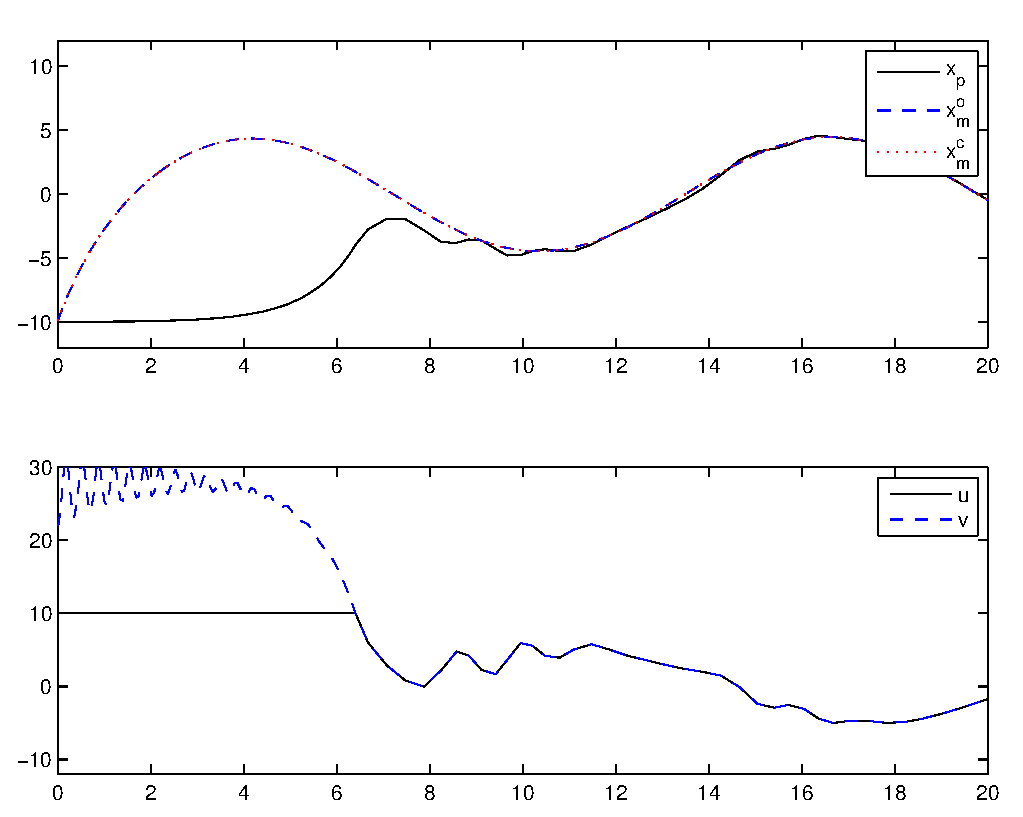
\includegraphics[width=3.0in]{\figurepath/fig1orm.eps}
    \caption{ORM:\ State and input}
  \end{center}
\end{figure}

\begin{figure}[H]
  \begin{center}
    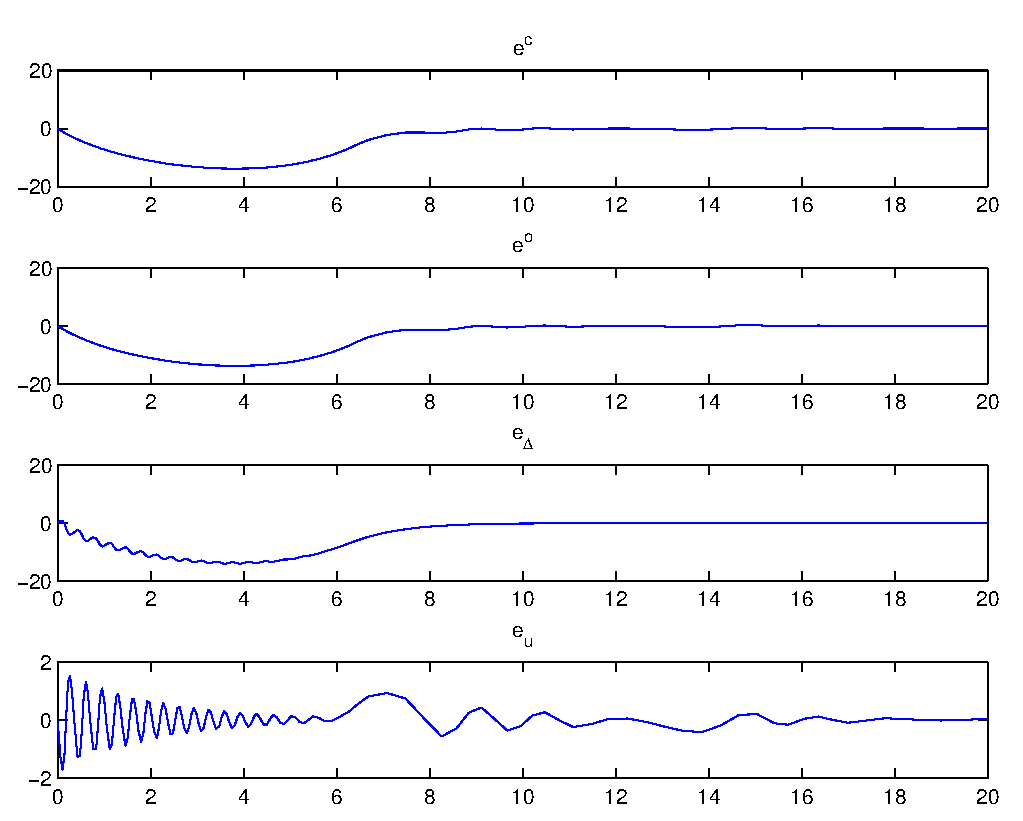
\includegraphics[width=3.0in]{\figurepath/fig2orm.eps}
    \caption{ORM:\ errors}
  \end{center}
\end{figure}

\begin{figure}[H]
  \begin{center}
    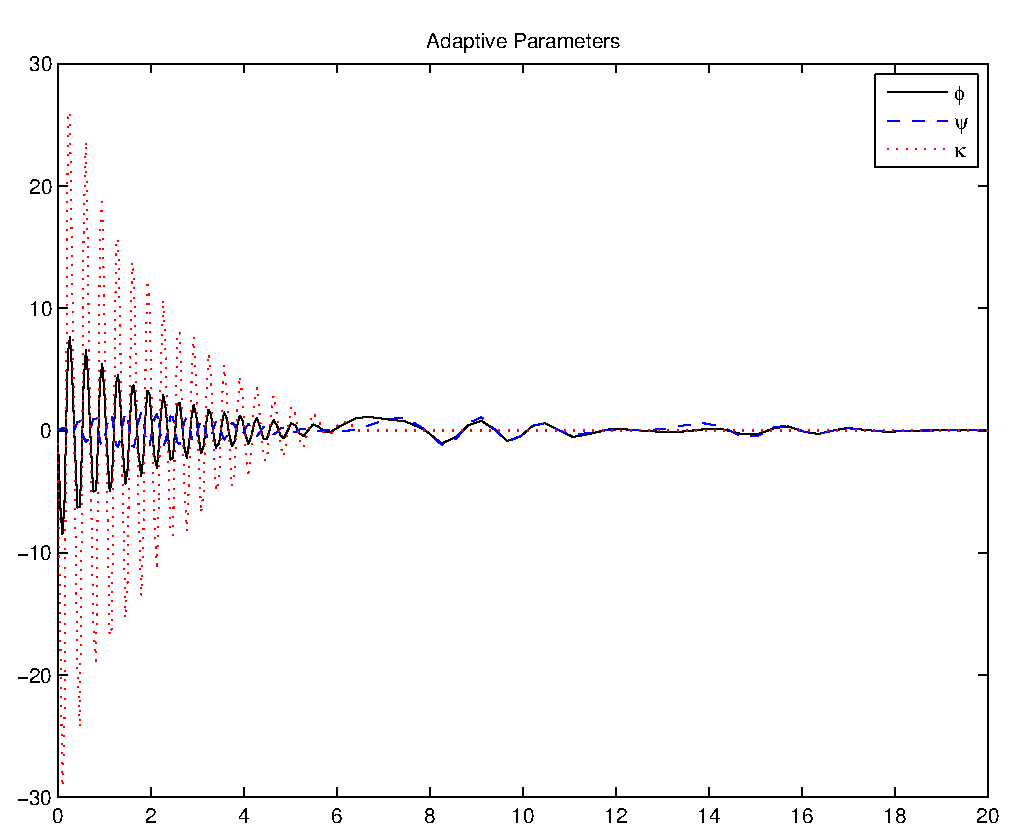
\includegraphics[width=3.0in]{\figurepath/fig3orm.eps}
    \caption{ORM:\ Parameters}
  \end{center}
\end{figure}

\subsection{Extension to Closed-Loop Reference Model}

Setting $\ell=0$ recovers the normal open-loop reference model case.
\begin{equation*}
  \dot{e}_{\Delta}=(a_{m}+\ell)e_{\Delta}+\beta_{\Delta}\Delta u
\end{equation*}
When the control input is saturating, the controller cannot achieve any higher level of performance.
That is, the controller should not seek to minimize an error signal which it is unable to do because of the limitation of the actuator.
Instead we define the error $e_{u}$ which takes the state error (the actual error we would like to minimize) and subtracts off the portion of the error due to the ``disturbance'' $\Delta u$ which the controller input can do nothing about.
This is the error we would like to use to drive adaptation.
If the controller is causing the input to saturate, there is no sense using an error signal which the controller cannot reduce to drive adaptation.
\begin{equation*}
  e_{u}=e^{c}-e_{\Delta}
\end{equation*}
The dynamics describing this error are given by
\begin{equation*}
  \dot{e}_{u}=\dot{e}^{c}-\dot{e}_{\Delta}
\end{equation*}
where, differentiating the state error
\begin{equation*}
  \dot{e}^{c}=\dot{x}_{p}-\dot{x}_{m}^{c}
\end{equation*}
plugging in
\begin{equation*}
  \dot{e}^{c}=a_{p}x_{p}+b_{p}u-a_{m}x_{m}^{c}-b_{m}r+\ell(x_{p}-x_{m}^{c})
\end{equation*}
Substituting in the control law $u=u_{c}+\Delta u$ and the matching conditions $a_{p}=a_{m}-b_{p}\theta^{*}$ and $b_{m}=b_{p}k^{*}$ we get
\begin{equation*}
  \dot{e}^{c}=(a_{m}-b_{p}\theta^{*})x_{p}+b_{p}(u_{c}+\Delta u)-a_{m}x_{m}^{c}-b_{p}k^{*}r+\ell(x_{p}-x_{m}^{c})
\end{equation*}
and then
\begin{equation*}
  \dot{e}^{c}=a_{m}x_{p}-b_{p}\theta^{*}x_{p}+b_{p}u_{c}+b_{p}\Delta u-a_{m}x_{m}^{c}-b_{p}k^{*}r+\ell x_{p}-\ell x_{m}^{c}
\end{equation*}
and then
\begin{equation*}
  \dot{e}^{c}=(a_{m}+\ell)(x_{p}-x_{m}^{c})-b_{p}\theta^{*}x_{p}+b_{p}u_{c}+b_{p}\Delta u-b_{p}k^{*}r
\end{equation*}
and now substituting the control law $u_{c}=\theta x_{p}+kr$ in
\begin{equation*}
  \dot{e}^{c}=(a_{m}+\ell)e^{c}-b_{p}\theta^{*}x_{p}+b_{p}\theta x_{p}+b_{p}kr+b_{p}\Delta u-b_{p}k^{*}r
\end{equation*}
and then
\begin{equation*}
  \dot{e}^{c}=(a_{m}+\ell)e^{c}+b_{p}(\theta-\theta^{*})x_{p}+b_{p}(k-k^{*})r+b_{p}\Delta u
\end{equation*}
Now define the following parameter errors
\begin{empheq}[box=\roomyfbox]{equation*}
  \tilde{\theta}=\theta-\theta^{*}
\end{empheq}
\begin{empheq}[box=\roomyfbox]{equation*}
  \tilde{k}=k-k^{*}
\end{empheq}
and substituting these in
\begin{equation*}
  \dot{e}^{c}=(a_{m}+\ell)e^{c}+b_{p}\tilde{\theta}x_{p}+b_{p}\tilde{k}r+b_{p}\Delta u
\end{equation*}
Now returning to $\dot{e}_{u}$
\begin{equation*}
  \dot{e}_{u}=(a_{m}+\ell)e^{c}+b_{p}\tilde{\theta}x_{p}+b_{p}\tilde{k}r+b_{p}\Delta u-(a_{m}+\ell)e_{\Delta}-\beta_{\Delta}\Delta u
\end{equation*}
and then
\begin{equation*}
  \dot{e}_{u}=(a_{m}+\ell)e_{u}+b_{p}\tilde{\theta}x_{p}+b_{p}\tilde{k}r+(b_{p}-\beta_{\Delta})\Delta u
\end{equation*}
and define the last parameter
\begin{empheq}[box=\roomyfbox]{equation*}
  \tilde{\beta}=b_{p}-\beta_{\Delta}
\end{empheq}
and then
\begin{equation*}
  \dot{e}_{u}=(a_{m}+\ell)e_{u}+b_{p}\tilde{\theta}x_{p}+b_{p}\tilde{k}r+\tilde{\beta}\Delta u
\end{equation*}
This is the error we want to try to minimize.
Now propose the following candidate Lyapunov function
\begin{empheq}[box=\roomyfbox]{equation*}
  V(e_{u},\tilde{\theta},\tilde{k},\tilde{\beta})=
  \frac{1}{2}e_{u}{}^{2}+
  \frac{1}{2}|b_{p}|\gamma_{1}^{-1}\tilde{\theta}^{2}+
  \frac{1}{2}|b_{p}|\gamma_{2}^{-1}\tilde{k}^{2}+
  \frac{1}{2}\gamma_{3}^{-1}\tilde{\beta}^{2}
\end{empheq}
taking the time derivative
\begin{equation*}
  \dot{V}=e_{u}\dot{e}_{u}+
  |b_{p}|\gamma_{1}^{-1}\tilde{\theta}\dot{\tilde{\theta}}+
  |b_{p}|\gamma_{2}^{-1}\tilde{k}\dot{\tilde{k}}+
  \gamma_{3}^{-1}\tilde{\beta}\dot{\tilde{\beta}}
\end{equation*}
substituting in $\dot{e}_{u}$
\begin{equation*}
  \dot{V}=e_{u}[(a_{m}+\ell)e_{u}+b_{p}\tilde{\theta}x_{p}+b_{p}\tilde{k}r+\tilde{\beta}\Delta u]+
  |b_{p}|\gamma_{1}^{-1}\tilde{\theta}\dot{\tilde{\theta}}+
  |b_{p}|\gamma_{2}^{-1}\tilde{k}\dot{\tilde{k}}+
  \gamma_{3}^{-1}\tilde{\beta}\dot{\tilde{\beta}}
\end{equation*}
and then
\begin{equation*}
  \dot{V}=(a_{m}+\ell)e_{u}{}^{2}+b_{p}\tilde{\theta}e_{u}x_{p}+b_{p}\tilde{k}e_{u}r+\tilde{\beta}e_{u}\Delta u+
  |b_{p}|\gamma_{1}^{-1}\tilde{\theta}\dot{\tilde{\theta}}+
  |b_{p}|\gamma_{2}^{-1}\tilde{k}\dot{\tilde{k}}+
  \gamma_{3}^{-1}\tilde{\beta}\dot{\tilde{\beta}}
\end{equation*}
Now the goal is to determine adaptive update laws for each of the parameters $\tilde{\theta}$, $\tilde{k}$, and $\tilde{\beta}$ such that all of the terms except the quadratic in $e_{u}$ are left.
That is
\begin{align*}
  b_{p}\tilde{\theta}e_{u}x_{p}+|b_{p}|\gamma_{1}^{-1}\tilde{\theta}\dot{\tilde{\theta}}=&0 \\
  b_{p}\tilde{k}e_{u}r+|b_{p}|\gamma_{2}^{-1}\tilde{k}\dot{\tilde{k}}=&0 \\
  \tilde{\beta}e_{u}\Delta u+\gamma_{3}^{-1}\tilde{\beta}\dot{\tilde{\beta}}=&0
\end{align*}
So this results in the following update laws
\begin{align*}
  \dot{\tilde{\theta}}&=-\gamma_{1}\text{sgn}(b_{p})e_{u}x_{p} \\
  \dot{\tilde{k}}&=-\gamma_{2}\text{sgn}(b_{p})e_{u}r \\
  \dot{\tilde{\beta}}&=-\gamma_{3}e_{u}\Delta u
\end{align*}
resulting in the following time derivative $\dot{V}$
\begin{equation*}
  \dot{V}=(a_{m}+\ell)e_{u}{}^{2}\leq0
\end{equation*}
And with $\dot{V}$ negative semi-definite, then $V$ is bounded above by $V(t_{0})$ and below by zero.
Additionally, the arguments of $V$ are also bounded for all $t\geq t_{0}$.

\subsubsection{Simulation Results}

\begin{figure}[H]
  \begin{center}
    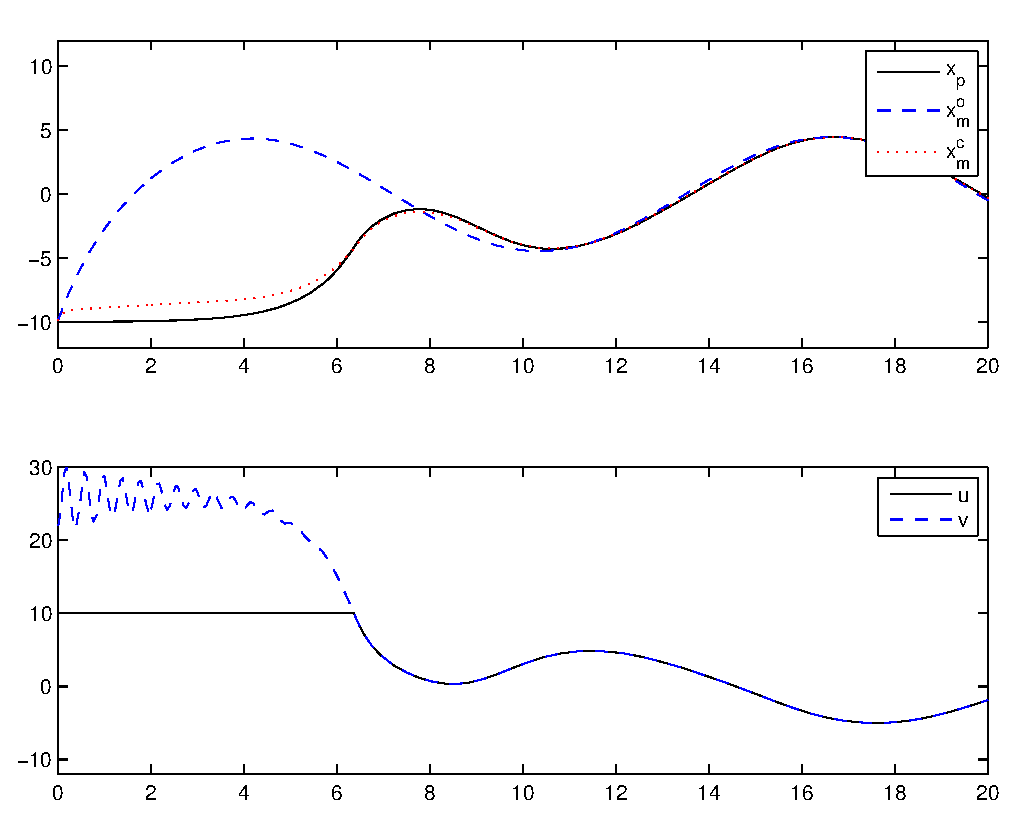
\includegraphics[width=3.0in]{\figurepath/fig1crm.eps}
    \caption{CRM:\ State and input}
  \end{center}
\end{figure}

\begin{figure}[H]
  \begin{center}
    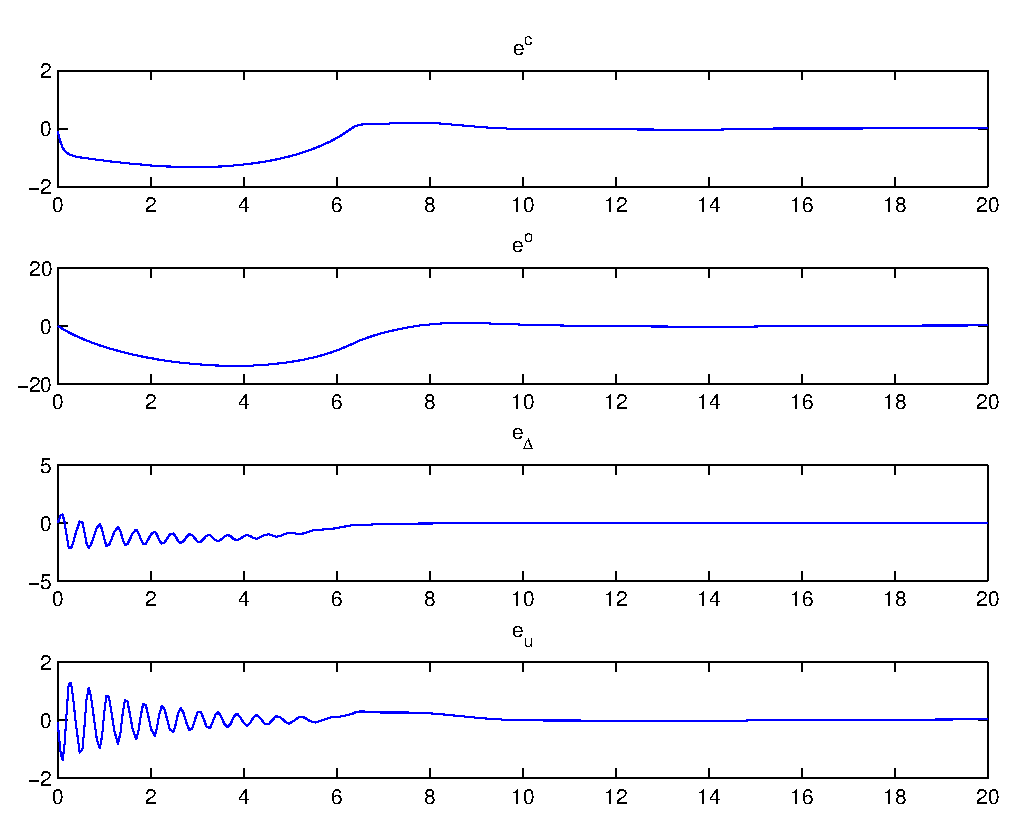
\includegraphics[width=3.0in]{\figurepath/fig2crm.eps}
    \caption{CRM:\ errors}
  \end{center}
\end{figure}

\begin{figure}[H]
  \begin{center}
    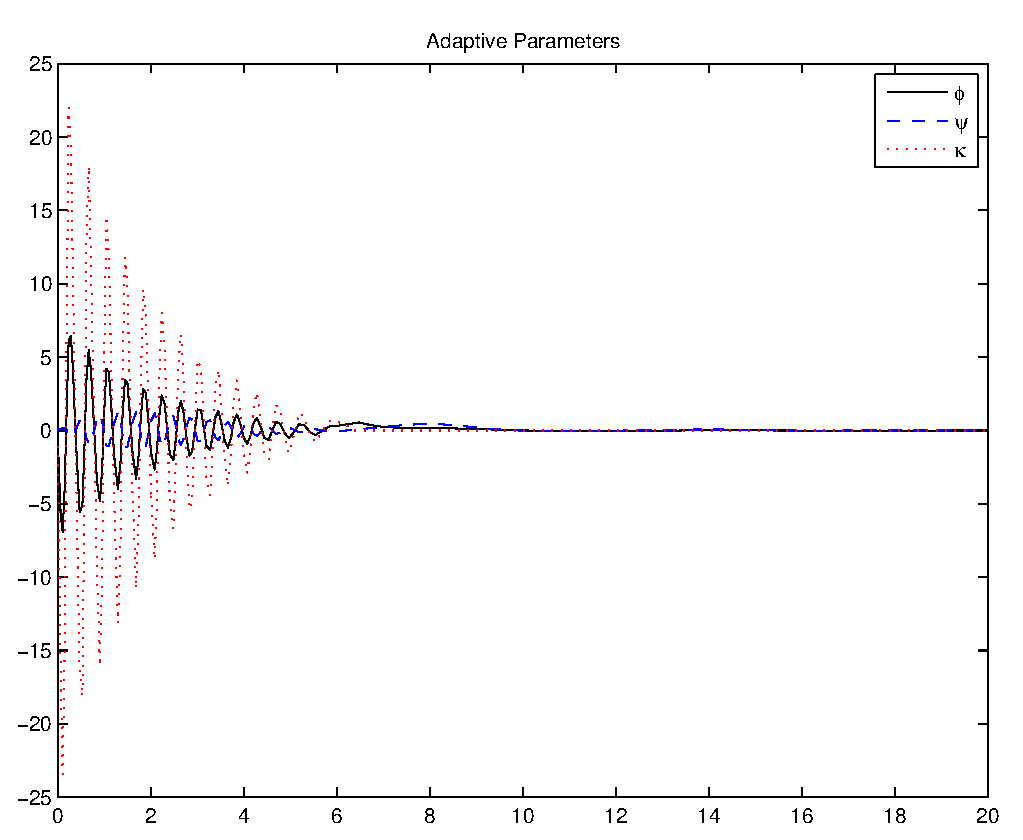
\includegraphics[width=3.0in]{\figurepath/fig3crm.eps}
    \caption{CRM:\ Parameters}
  \end{center}
\end{figure}

\subsection{Saturation Protection Higher Order with CRM}

Plant to be controlled
\begin{equation*}
  \dot{x}=(A+B_{1}\Lambda W^{\mathsf{T}})x+B_{1}\Lambda u+B_{2}x_{\text{cmd}}
\end{equation*}
commanded control law
\begin{equation*}
  u_{c}=(\theta+K_{x})^{\mathsf{T}}x
\end{equation*}
actual control input to the plant due to the position saturation of the actuators
\begin{equation*}
  u=
  \begin{cases}
    u_{c} &\mbox{if } |u_{c}|\leq u_{\text{max}} \\
    u_{\text{max}}\text{sgn}(u_{c}) & \mbox{if } |u_{c}|>u_{\text{max}}
  \end{cases}
\end{equation*}
$\Delta u$ is the control deficit.
\begin{empheq}[box=\roomyfbox]{equation*}
  u=u_{c}+\Delta{} u
\end{empheq}
Plugging in the control into the plant equation and $r=x_{\text{cmd}}$
\begin{equation*}
  \dot{x}=(A+B_{1}\Lambda W^{\mathsf{T}})x+B_{1}\Lambda(u_{c}+\Delta u)+B_{2}r
\end{equation*}
and then
\begin{equation*}
  \dot{x}=(A+B_{1}\Lambda W^{\mathsf{T}})x+B_{1}\Lambda u_{c}+B_{1}\Lambda\Delta u+B_{2}r
\end{equation*}
The reference model is given by
\begin{equation*}
  \dot{x}_{m}^{c}=A_{m}x_{m}^{c}+B_{m}x_{\text{cmd}}-L(x-x_{m}^{c})
\end{equation*}
\begin{equation*}
  \dot{x}_{m}^{c}=A_{m}x_{m}^{c}+B_{2}r-L(x-x_{m}^{c})
\end{equation*}
where
\begin{equation*}
  A_{m}=A+B_{1}K_{x}^{\mathsf{T}}
\end{equation*}
I am using a closed-loop reference model
\begin{empheq}[box=\roomyfbox]{equation*}
  \dot{e}_{\Delta}=(A_{m}+L)e_{\Delta}+\beta_{\Delta}\Delta{} u
\end{empheq}
and
\begin{empheq}[box=\roomyfbox]{equation*}
  e_{u}=e^{c}-e_{\Delta}
\end{empheq}
The dynamics describing this error are given by
\begin{equation*}
  \dot{e}_{u}=\dot{e}^{c}-\dot{e}_{\Delta}
\end{equation*}
where, differentiating the state error
\begin{equation*}
  \dot{e}^{c}=\dot{x}-\dot{x}_{m}^{c}
\end{equation*}
plugging in
\begin{equation*}
  \dot{e}^{c}=(A+B_{1}\Lambda W^{\mathsf{T}})x+B_{1}\Lambda u_{c}+B_{1}\Lambda\Delta u+B_{2}r-
  [A_{m}x_{m}^{c}+B_{2}r-L(x-x_{m}^{c})]
\end{equation*}
and then
\begin{equation*}
  \dot{e}^{c}=(A+B_{1}\Lambda W^{\mathsf{T}})x+B_{1}\Lambda u_{c}+B_{1}\Lambda\Delta u-
  A_{m}x_{m}^{c}+L(x-x_{m}^{c})
\end{equation*}
Using $A=A_{m}-B_{1}K_{x}^{\mathsf{T}}$ and $u_{c}=(\theta+K_{x})^{\mathsf{T}}x$
\begin{equation*}
  \dot{e}^{c}=(A_{m}-B_{1}K_{x}^{\mathsf{T}}+B_{1}\Lambda W^{\mathsf{T}})x+B_{1}\Lambda(\theta+K_{x})^{\mathsf{T}}x+B_{1}\Lambda\Delta u-
  A_{m}x_{m}^{c}+L(x-x_{m}^{c})
\end{equation*}
and then
\begin{equation*}
  \dot{e}^{c}=A_{m}x+(-B_{1}K_{x}^{\mathsf{T}}+B_{1}\Lambda W^{\mathsf{T}})x+B_{1}\Lambda\theta^{\mathsf{T}}x+B_{1}\Lambda K_{x}^{\mathsf{T}}x+B_{1}\Lambda\Delta u-A_{m}x_{m}^{c}+L(x-x_{m}^{c})
\end{equation*}
and then
\begin{equation*}
  \dot{e}^{c}=A_{m}(x-x_{m}^{c})+(B_{1}\Lambda\theta^{\mathsf{T}}+B_{1}\Lambda K_{x}^{\mathsf{T}}-B_{1}K_{x}^{\mathsf{T}}+B_{1}\Lambda W^{\mathsf{T}})x+B_{1}\Lambda\Delta u+L(x-x_{m}^{c})
\end{equation*}
and then
\begin{equation*}
  \dot{e}^{c}=(A_{m}+L)(x-x_{m}^{c})+(B_{1}\Lambda\theta^{\mathsf{T}}+B_{1}\Lambda K_{x}^{\mathsf{T}}-B_{1}K_{x}^{\mathsf{T}}+B_{1}\Lambda W^{\mathsf{T}})x+B_{1}\Lambda\Delta u
\end{equation*}
and then
\begin{equation*}
  \dot{e}^{c}=(A_{m}+L)(x-x_{m}^{c})+B_{1}(\Lambda\theta^{\mathsf{T}}+\Lambda K_{x}^{\mathsf{T}}-K_{x}^{\mathsf{T}}+\Lambda W^{\mathsf{T}})x+B_{1}\Lambda\Delta u
\end{equation*}
and from the matching condition we have
\begin{equation*}
  \Lambda\left[W^{\mathsf{T}}+(\theta^{*}+K_{x})^{\mathsf{T}}\right]=K_{x}^{\mathsf{T}}
\end{equation*}
which we can rearrange
\begin{equation*}
  \Lambda W^{\mathsf{T}}+\Lambda\theta^{*\mathsf{T}}+\Lambda K_{x}^{\mathsf{T}}=K_{x}^{\mathsf{T}}
\end{equation*}
and then
\begin{equation*}
  \Lambda K_{x}^{\mathsf{T}}-K_{x}^{\mathsf{T}}+\Lambda W^{\mathsf{T}}=-\Lambda\theta^{*\mathsf{T}}
\end{equation*}
substituting this in
\begin{equation*}
  \dot{e}^{c}=(A_{m}+L)(x-x_{m}^{c})+B_{1}(\Lambda\theta^{\mathsf{T}}-\Lambda\theta^{*\mathsf{T}})x+B_{1}\Lambda\Delta u
\end{equation*}
and with $\tilde{\theta}=\theta-\theta^{*}$ we get
\begin{equation*}
  \dot{e}^{c}=(A_{m}+L)(x-x_{m}^{c})+B_{1}\Lambda\tilde{\theta}^{\mathsf{T}}x+B_{1}\Lambda\Delta u
\end{equation*}
\begin{equation*}
  \dot{e}^{c}=(A_{m}+L)e^{c}+B_{1}\Lambda\tilde{\theta}^{\mathsf{T}}x+B_{1}\Lambda\Delta u
\end{equation*}
And using $\dot{e}_{u}=\dot{e}^{c}-\dot{e}_{\Delta}$
\begin{equation*}
  \dot{e}_{u}=(A_{m}+L)e^{c}+B_{1}\Lambda\tilde{\theta}^{\mathsf{T}}x+B_{1}\Lambda\Delta u-
  [(A_{m}+L)e_{\Delta}+\beta_{\Delta}\Delta u]
\end{equation*}
and then
\begin{equation*}
  \dot{e}_{u}=(A_{m}+L)e^{c}+B_{1}\Lambda\tilde{\theta}^{\mathsf{T}}x+B_{1}\Lambda\Delta u-
  (A_{m}+L)e_{\Delta}-\beta_{\Delta}\Delta u
\end{equation*}
and then
\begin{equation*}
  \dot{e}_{u}=(A_{m}+L)(e^{c}-e_{\Delta})+B_{1}\Lambda\tilde{\theta}^{\mathsf{T}}x+B_{1}\Lambda\Delta u-\beta_{\Delta}\Delta u
\end{equation*}
and then
\begin{equation*}
  \dot{e}_{u}=(A_{m}+L)e_{u}+B_{1}\Lambda\tilde{\theta}^{\mathsf{T}}x+(B_{1}\Lambda-\beta_{\Delta})\Delta u
\end{equation*}
defining $\tilde{\beta}=B_{1}\Lambda-\beta_{\Delta}$ we get the following augmented error dynamics
\begin{equation*}
  \dot{e}_{u}=(A_{m}+L)e_{u}+B_{1}\Lambda\tilde{\theta}^{\mathsf{T}}x+\tilde{\beta}\Delta u
\end{equation*}
\begin{empheq}[box=\roomyfbox]{equation*}
  \dot{e}_{u}=\bar{A}_{m}e_{u}+B_{1}\Lambda\tilde{\theta}^{\mathsf{T}}x+\tilde{\beta}\Delta{} u
\end{empheq}
Proposing the following candidate Lyapunov function
\begin{empheq}[box=\roomyfbox]{equation*}
  V=e_{u}^{\mathsf{T}}Pe_{u}+
  \text{tr}\left(\tilde{\theta}^{\mathsf{T}}\Gamma^{-1}\tilde{\theta}|\Lambda|\right)+
  \tilde{\beta}^{\mathsf{T}}\Gamma_{\beta}^{-1}\tilde{\beta}
\end{empheq}
Differentiating
\begin{equation*}
  \dot{V}={\dot{e}}_{u}^{\mathsf{T}}Pe_{u}+e_{u}^{\mathsf{T}}P\dot{e}_{u}+
  \text{tr}(\dot{\tilde{\theta}}^{\mathsf{T}}\Gamma^{-1}\tilde{\theta}|\Lambda|)+
  \text{tr}({\tilde{\theta}}^{\mathsf{T}}\Gamma^{-1}\dot{\tilde{\theta}}|\Lambda|)+
  \dot{\tilde{\beta}}^{\mathsf{T}}\Gamma_{\beta}^{-1}\tilde{\beta}+
  \tilde{\beta}^{\mathsf{T}}\Gamma_{\beta}^{-1}\dot{\tilde{\beta}}
\end{equation*}
Substituting error dynamics equation from above, with the transpose
\begin{equation*}
  \dot{e}_{u}^{\mathsf{T}}=e_{u}^{\mathsf{T}}\bar{A}_{m}^{\mathsf{T}}+x^{\mathsf{T}}\tilde{\theta}\Lambda B_{1}^{\mathsf{T}}+\Delta u^{\mathsf{T}}\tilde{\beta}^{\mathsf{T}}
\end{equation*}
and simplifying
\begin{equation*}
  \dot{V}
  =(e_{u}^{\mathsf{T}}\bar{A}_{m}^{\mathsf{T}}+x^{\mathsf{T}}\tilde{\theta}\Lambda B_{1}^{\mathsf{T}}
  +\Delta u^{\mathsf{T}}\tilde{\beta}^{\mathsf{T}})Pe_{u}+e_{u}^{\mathsf{T}}P(\bar{A}_{m}e_{u}
  +B_{1}\Lambda\tilde{\theta}^{\mathsf{T}}x+\tilde{\beta}\Delta u)
  +\text{tr}(\dot{\tilde{\theta}}^{\mathsf{T}}\Gamma^{-1}\tilde{\theta}|\Lambda|)
  +\text{tr}({\tilde{\theta}}^{\mathsf{T}}\Gamma^{-1}\dot{\tilde{\theta}}|\Lambda|)
  +\dot{\tilde{\beta}}^{\mathsf{T}}\Gamma_{\beta}^{-1}\tilde{\beta}
  +\tilde{\beta}^{\mathsf{T}}\Gamma_{\beta}^{-1}\dot{\tilde{\beta}}
\end{equation*}
and then
\begin{equation*}
  \dot{V}=(e_{u}^{\mathsf{T}}\bar{A}_{m}^{\mathsf{T}}Pe_{u})+
  (x^{\mathsf{T}}\tilde{\theta}\Lambda B_{1}^{\mathsf{T}}+\Delta u^{\mathsf{T}}\tilde{\beta}^{\mathsf{T}})Pe_{u}+
  (e_{u}^{\mathsf{T}}P\bar{A}_{m}e_{u})+
  e_{u}^{\mathsf{T}}P(B_{1}\Lambda\tilde{\theta}^{\mathsf{T}}x+\tilde{\beta}\Delta u)+
  \text{tr}(\dot{\tilde{\theta}}^{\mathsf{T}}\Gamma^{-1}\tilde{\theta}|\Lambda|)+
  \text{tr}({\tilde{\theta}}^{\mathsf{T}}\Gamma^{-1}\dot{\tilde{\theta}}|\Lambda|)+
  \dot{\tilde{\beta}}^{\mathsf{T}}\Gamma_{\beta}^{-1}\tilde{\beta}+
  \tilde{\beta}^{\mathsf{T}}\Gamma_{\beta}^{-1}\dot{\tilde{\beta}}
\end{equation*}
and then
\begin{equation*}
  \dot{V}=e_{u}^{\mathsf{T}}(\bar{A}_{m}^{\mathsf{T}}P+P\bar{A}_{m})e_{u}+
  (x^{\mathsf{T}}\tilde{\theta}\Lambda B_{1}^{\mathsf{T}}+\Delta u^{\mathsf{T}}\tilde{\beta}^{\mathsf{T}})Pe_{u}+
  e_{u}^{\mathsf{T}}P(B_{1}\Lambda\tilde{\theta}^{\mathsf{T}}x+\tilde{\beta}\Delta u)+
  \text{tr}(\dot{\tilde{\theta}}^{\mathsf{T}}\Gamma^{-1}\tilde{\theta}|\Lambda|)+
  \text{tr}({\tilde{\theta}}^{\mathsf{T}}\Gamma^{-1}\dot{\tilde{\theta}}|\Lambda|)+
  \dot{\tilde{\beta}}^{\mathsf{T}}\Gamma_{\beta}^{-1}\tilde{\beta}+
  \tilde{\beta}^{\mathsf{T}}\Gamma_{\beta}^{-1}\dot{\tilde{\beta}}
\end{equation*}
and with $\bar{A}_{m}^{\mathsf{T}}P+P\bar{A}_{m}=-Q$ we get
\begin{equation*}
  \dot{V}=-e_{u}^{\mathsf{T}}Qe_{u}+
  x^{\mathsf{T}}\tilde{\theta}\Lambda B_{1}^{\mathsf{T}}Pe_{u}+
  \Delta u^{\mathsf{T}}\tilde{\beta}^{\mathsf{T}}Pe_{u}+
  e_{u}^{\mathsf{T}}PB_{1}\Lambda\tilde{\theta}^{\mathsf{T}}x+
  e_{u}^{\mathsf{T}}P\tilde{\beta}\Delta u+
  \text{tr}(\dot{\tilde{\theta}}^{\mathsf{T}}\Gamma^{-1}\tilde{\theta}|\Lambda|)+
  \text{tr}({\tilde{\theta}}^{\mathsf{T}}\Gamma^{-1}\dot{\tilde{\theta}}|\Lambda|)+
  \dot{\tilde{\beta}}^{\mathsf{T}}\Gamma_{\beta}^{-1}\tilde{\beta}+
  \tilde{\beta}^{\mathsf{T}}\Gamma_{\beta}^{-1}\dot{\tilde{\beta}}
\end{equation*}
since the terms of $\dot{V}$ are all scalars we have
\begin{equation*}
  \dot{V}=-e_{u}^{\mathsf{T}}Qe_{u}+
  2x^{\mathsf{T}}\tilde{\theta}\Lambda B_{1}^{\mathsf{T}}Pe_{u}+
  2 \Delta u^{\mathsf{T}}\tilde{\beta}^{\mathsf{T}}Pe_{u}+
  \text{tr}(\dot{\tilde{\theta}}^{\mathsf{T}}\Gamma^{-1}\tilde{\theta}|\Lambda|)+
  \text{tr}({\tilde{\theta}}^{\mathsf{T}}\Gamma^{-1}\dot{\tilde{\theta}}|\Lambda|)+
  2\tilde{\beta}^{\mathsf{T}}\Gamma_{\beta}^{-1}\dot{\tilde{\beta}}
\end{equation*}
The following adaptive control gain update laws are proposed
\begin{empheq}[box=\roomyfbox]{equation*}
  \dot{\theta}=\text{Proj}_{\Gamma}(\theta,-\Gamma{} xe_{u}^{\mathsf{T}}PB_{1}\text{sgn}(\Lambda))
\end{empheq}
\begin{empheq}[box=\roomyfbox]{equation*}
  \dot{\tilde{\beta}}=-\Gamma_{\beta}Pe_{u}\Delta{} u
\end{empheq}
Looking at only the $\tilde{\beta}$ terms
\begin{equation*}
  2 \Delta u^{\mathsf{T}}\tilde{\beta}^{\mathsf{T}}Pe_{u}-
  2\tilde{\beta}^{\mathsf{T}}\Gamma_{\beta}^{-1}\Gamma_{\beta}Pe_{u}\Delta u=
\end{equation*}
and since we are considering scalar input system
\begin{equation*}
  2 \Delta u^{\mathsf{T}}\tilde{\beta}^{\mathsf{T}}Pe_{u}-
  2\Delta u \tilde{\beta}^{\mathsf{T}}Pe_{u}=0
\end{equation*}
and so $\dot{V}$ becomes
\begin{equation*}
  \dot{V}=-e_{u}^{\mathsf{T}}Qe_{u}+
  2x^{\mathsf{T}}\tilde{\theta}\Lambda B_{1}^{\mathsf{T}}Pe_{u}+
  \text{tr}(\dot{\tilde{\theta}}^{\mathsf{T}}\Gamma^{-1}\tilde{\theta}|\Lambda|)+
  \text{tr}({\tilde{\theta}}^{\mathsf{T}}\Gamma^{-1}\dot{\tilde{\theta}}|\Lambda|)
\end{equation*}
using $\text{tr}(a)=\text{tr}(a^{\mathsf{T}})$, $\Lambda=\Lambda^{\mathsf{T}}$, $\Gamma=\Gamma^{\mathsf{T}}$, and $\text{tr}(ab)=\text{tr}(ba)$ we get
\begin{equation*}
  \dot{V}=-e_{u}^{\mathsf{T}}Qe+2x^{\mathsf{T}}{\tilde{\theta}}\Lambda{B_{1}}^{\mathsf{T}}Pe_{u}
  +2\text{tr}({\tilde{\theta}}^{\mathsf{T}}\Gamma^{-1}\dot{\tilde{\theta}}|\Lambda|) \\
\end{equation*}
Substituting the adaptive control gain update law for $\theta$
\begin{equation*}
  \dot{V}=-e_{u}^{\mathsf{T}}Qe+2x^{\mathsf{T}}{\tilde{\theta}}\Lambda{B_{1}}^{\mathsf{T}}Pe_{u}
  +2\text{tr}\left({\tilde{\theta}}^{\mathsf{T}}\Gamma^{-1}\text{Proj}_{\Gamma}(\theta,-\Gamma xe_{u}^{\mathsf{T}}PB_{1}\text{sgn}(\Lambda))|\Lambda|\right) \\
\end{equation*}
Since the quantity $2x^{\mathsf{T}}{\tilde{\theta}}\Lambda{B_{1}}^{\mathsf{T}}Pe_{u}$ is scalar, it is equal to its trace, so we can write
\begin{equation*}
  \dot{V}=-e_{u}^{\mathsf{T}}Qe_{u}+2\text{tr}(x^{\mathsf{T}}{\tilde{\theta}}\Lambda{B_{1}}^{\mathsf{T}}Pe_{u})
  +2\text{tr}\left({\tilde{\theta}}^{\mathsf{T}}\Gamma^{-1}\text{Proj}_{\Gamma}(\theta,-\Gamma xe_{u}^{\mathsf{T}}PB_{1}\text{sgn}(\Lambda))|\Lambda|\right) \\
\end{equation*}
The terms inside the first trace operator can be rearranged using $\text{tr}(a)=\text{tr}(a^{\mathsf{T}})$, $\Lambda=\Lambda^{\mathsf{T}}$, and $\text{tr}(ab)=\text{tr}(ba)$
\begin{equation*}
  \dot{V}=-e_{u}^{\mathsf{T}}Qe_{u}+2\text{tr}(\tilde{\theta}^{\mathsf{T}}xe_{u}^{\mathsf{T}}PB_{1}\Lambda)
  +2\text{tr}\left({\tilde{\theta}}^{\mathsf{T}}\Gamma^{-1}\text{Proj}_{\Gamma}(\theta,-\Gamma xe_{u}^{\mathsf{T}}PB_{1}\text{sgn}(\Lambda))|\Lambda|\right) \\
\end{equation*}
Combining the trace operators
\begin{equation*}
  \dot{V}=-e_{u}^{\mathsf{T}}Qe_{u}
  +2\text{tr}\left(\tilde{\theta}^{\mathsf{T}}xe^{\mathsf{T}}PB_{1}\Lambda+
  {\tilde{\theta}}^{\mathsf{T}}\Gamma^{-1}\text{Proj}_{\Gamma}(\theta,-\Gamma xe_{u}^{\mathsf{T}}PB_{1}\text{sgn}(\Lambda))|\Lambda|\right) \\
\end{equation*}
\begin{equation*}
  \dot{V}=-e_{u}^{\mathsf{T}}Qe_{u}
  +2\text{tr}\left(\tilde{\theta}^{\mathsf{T}}\left(\Gamma^{-1}\text{Proj}_{\Gamma}(\theta,-\Gamma xe_{u}^{\mathsf{T}}PB_{1}\text{sign}(\Lambda))|\Lambda|+xe_{u}^{\mathsf{T}}PB_{1}\Lambda\right)\right) \\
\end{equation*}
Let $y=-xe_{u}^{\mathsf{T}}PB_{1}\text{sign}(\Lambda)$ and with $\text{sign}(\Lambda)|\Lambda|=\Lambda$
\begin{equation*}
  \dot{V}=-e_{u}^{\mathsf{T}}Qe_{u}
  +2\text{tr}\left(\tilde{\theta}^{\mathsf{T}}\left(\Gamma^{-1}\text{Proj}_{\Gamma}(\theta,\Gamma y)|\Lambda|-y|\Lambda|\right)\right)
\end{equation*}
\begin{equation*}
  \dot{V}=-e_{u}^{\mathsf{T}}Qe_{u}
  +2\text{tr}\left(\tilde{\theta}^{\mathsf{T}}\left(\Gamma^{-1}\text{Proj}_{\Gamma}(\theta,\Gamma y)-y\right)|\Lambda|\right)
\end{equation*}
And we have the following inequality (See my personal notes)
\begin{equation*}
  \tilde{\theta}^{\mathsf{T}}(\Gamma^{-1}\text{Proj}_{\Gamma}(\theta,\Gamma y)-y)\leq 0
\end{equation*}
So, if a symmetric, positive definite matrix $P$ exists, which solves the Lyapunov equation $\bar{A}_{m}{}^{\mathsf{T}}P+P\bar{A}_{m}+Q=0$, where $Q$ is positive definite, then $\dot{V}=\dot{V}(e,\theta)\leq 0$ is negative semidefinite, and $V(e,\theta)$ serves as a valid Lyapunov function for this system.

\chapter{Appendix}

\begin{example}
\begin{center}
\begin{tikzpicture}[auto, scale=0.9, every node/.style={transform shape}, node distance=1.0cm, >=latex']
\node[input](input1){};
\node[tee, right of= input1, node distance=1.0cm](tee2){};
\node[tee, above of= tee2, node distance=1.5cm](tee3){};
\node[tee, below of= tee2, node distance=1.5cm](tee4){};
\node[tee, right of=tee4,node distance=0.0cm] (block1){};
\node[squareblock, right of= block1, node distance=2.0cm](sum1){\shortstack{Adaptive \\  Controller}};
\node[squareblock, right of=sum1,label=above:{},node distance=3.0cm] (block2){\shortstack{Plant}};
\node[squareblock, above of=block2,label=below:{},label=above:{},node distance=3.0cm] (block3){\shortstack{Reference \\ Model}};
\node[tee, left of= block3, node distance=2.0cm](sum3){};
\node[roundblock, above of=block2,node distance=1.5cm] (block4){$\Theta$};
\node[whitesum, right of= tee2,node distance=9.0cm](sum2){};
\node[roundblock, above of=sum2,node distance=3.0cm] (block5){$L$};
\node[output, right of=sum2, node distance=2.5cm](output1){};
%Draw
\draw[-](input1) -- node[near start]{$z_{\text{cmd}}$} node[pos=0.7] {} (tee2);
\draw[-](tee2) -- (tee3);
\draw[-](tee2) -- (tee4);
\draw[->](tee3) -- node[pos=0.9]{} (block3);
%\draw[-](sum3) -- (block3);
\draw[-](tee4) -- (block1);
\draw[->](block1) -- node[near end] {} (sum1);
\draw[->](sum1) -- (block2);
\draw[->](block3) -| node[near start]{$x_{m}$} node[pos=0.3,name=xm]{} node[near end] {$-$} (sum2);
\draw[->](block2) -| node[near start]{$x$} node[pos=0.3,name=xp]{} node[pos=0.9] {$+$} (sum2);
\draw[->](xm) |- (block4);
\draw[->](block4) -| node[pos=0.9]{} (sum1);
\draw[->](sum2) -- node[near end]{$e$} node[pos=0.5, name=e, below]{} (output1);
\draw[->](e) |- (block5);
\draw[->](block5) -| node[pos=0.9]{} (block3);
%%Adaptive Arrow
%\coordinate (arrow1) at ([xshift=-0.7cm,yshift=-0.7cm] block1);
%\coordinate (arrow2) at (block1.225);
%\coordinate (arrow3) at (block1.45);
%\coordinate (arrow4) at ([xshift=0.7cm,yshift=0.7cm] block1);
%\draw[-](arrow1) -- (arrow2);
%\draw[->](arrow3) -- (arrow4);
%Adaptive Arrow
\coordinate (arrow1) at ([xshift=-0.7cm,yshift=-0.7cm] block4);
\coordinate (arrow2) at (block4.225);
\coordinate (arrow3) at (block4.45);
\coordinate (arrow4) at ([xshift=0.7cm,yshift=0.7cm] block4);
\draw[-](arrow1) -- (arrow2);
\draw[->](arrow3) -- (arrow4);
\end{tikzpicture}
\end{center}
\end{example}


\section{Eugene Lecture}

Last class $n^{*}\geq2$

EUGENE STUFF

Linear Control
LQR (state feedback)
PID (classical, output)
H-inf (both)
Pole placement (state feedback)
LQG (LQG+kalman filter/estimator)

Nonlinear Control
SMC (variable structure control)
- good for DC motor control, bad for flight control
Feedback linearization (dynamic inversion, works great in Matlab, not good in real life\ldots
no guarantees for robustness)
Lyapunov redesign (mostly for systems with known dynamics, adaptive could kinda be considered to fall under here)
Adaptive control

all the control strategies above are model based design/analysis

Plant --> model
Models are all incorrect\ldots
Some more than others.
Use model to cook up control, hoping that even though model is incorrect the control will work on plant
Plant --> model --> controller

reason this works is robustness.
Robustness is the key.

Dynamic inversion very sensitive.
Dynamic inversion might work, but can take a lot of time to design analyze and tune.

$H_{\infty}$ control on Harrier\ldots

\begin{example}[X-45A]
  super unstable.
  Time to departure 20ms.
  3 gains in pitch
  5 gains in roll/yaw
  used LQR control.
\end{example}

pretty much everything Boeing does (80\textemdash{}90 percent) is LQR

Adaptive control.
Does it work? yes.
Does it always work? no!

build robust control (e.g.
LQR)

to fly all we need is 40* phase margin and 8dB gain margin.

LQR is really good for uncertainties in $A$ and $B$ but is highly sensitive when $A$ and $B$ are state dependent.
For example, standing shock wave on top of delta wing as it moves with changes in flight condition.

LQR controller has no tolerance to ``bubbles'' in, for example, pitching moment versus elevator angle plot because of shock wave.

\section{Dr.\ Annaswamy Lecturing}

SISO system

u to y through plant P

P is of form $W_{p}(s)=\frac{k_{p}Z_{p}(s)}{R_{p}(s)}$

degrees of freedom\ldots
Filters of dimension $n-1$

Error model

Introduce auxiliary error $e_{2}$, augmented error $\varepsilon_{1}$ where $\varepsilon_{1}=e_{1}+e_{2}$.
Use $\varepsilon_{1}$ instead of $e_{1}$ in adaptive law.

Omega in through $W_{m}(s)$ and get $\zeta$ then use $\dot{\theta}=-\varepsilon_{1}\zeta$

SHOW BLOCK DIAGRAM THAT GENERATES $e_{2}$.

BLOCK DIAGRAM FOR ANALYTIC PART, THAT ALGEBRAIC PART CANCELS

when $e_{1}+e_{2}$:\ $W_{m}(s)[\tilde{\theta}^{\top}]$ $+\tilde{\theta}^{\top}\zeta-W_{m}(s)[\tilde{\theta}^{\top}\omega]$ and assume for simplicity that $k^{*}=1$ and so we get $\varepsilon_{1}=\tilde{\theta}^{\top}\zeta$.
So now use $\dot{\tilde{\theta}}=-\varepsilon_{1}\zeta$.

Started out with adaptive system which was nonlinear and time-varying.
And $\tilde{\theta}$ is bounded so this is reduced to a linear time-varying system.
Can we then use this to prove stability? Need to take one more step.

Need to allow $\tilde{\theta}$ to grow slowly.
Make it the normalized quantity.

\section{Review}

Class review

control of an uncertain dynamic system:\ adaptive control

two bins:
\begin{enumerate}
  \setlength{\itemsep}{0pt}
  \item{Input, states, output}
  \item{parameters}
\end{enumerate}

in adaptive control measure as many of (1) as possible, and deal with as many in (2) as possible
must assume there is a plant model, and since parameters are being attached to the model, must assume the structure of the model is known

one unifying theme of adaptive control/identificaation:\ error model

Two classes of error:
\begin{enumerate}
  \setlength{\itemsep}{0pt}
  \item{parameter}
  \item{tracking}
\end{enumerate}

error model is ``black box'' between parameter error and tracking error.
Want this black box to have a nice feature to \ldots

\begin{enumerate}
  \setlength{\itemsep}{0pt}
  \item{error model 1:\ $e=\omega\tilde{\theta}$ $e$ is linear regression of $\tilde{\theta}$}
  \item{error model 2:\ dynamics between parameter error and $e$ $w=\omega\tilde{\theta}$ then $w$ goes into $\dot{e}=Ae+Bw$}
  \item{%
    error model 3:\ specific case of error model 2, and now only some part of the error is available $e_{1}$.
    And we needed dynamics to be SPR.\@
  }
  \item{error model 4:\ uses augmented error approach with adding and subtracting\ldots
  for arbitrary relative degree.
  Add $e_{1}$ and $e_{2}$ to get $\varepsilon_{1}$}
\end{enumerate}

Adaptive Control
(1) First order plant
$\frac{1}{s-a_{p}}$
so know model structure (its first order)
put $\theta$ in feedback
error model becomes $x_{p}$ -> $\tilde{\theta}$ -> $\frac{1}{s-a_{m}}$ -> $e$
$\dot{\tilde{\theta}}=-ex_{p}$

extend to $\frac{k_{p}}{s-a_{p}}$ where $k_{p}$ has known sign, by adding a feedforward part
error model becomes $\omega$ -> $\tilde{\theta}$ -> $\frac{k_{p}}{s-a_{m}}$ -> $e$
$\omega=[r x_{p}]^{\top}$
$\dot{\tilde{\theta}}=-sgn(k_{p})e\omega$

(2) States accessible
$\dot{x}_{p}=A_{p}x_{p}+Bu$
$B\Lambda^{*}=B_{m}$ where $\Lambda^{*}$ is diagonal with the sign of each of the elements on the diagonal is known.
$\omega=[r^{\top} x_{p}^{\top}]^{\top}$
$\omega$ -> $\tilde{\theta}$ -> box -> $e$
$\dot{\tilde{\theta}}=-sgn(\Lambda^{*})\omega e^{\top}PB_{m}$

Adaptive Control:\ PI, PID, Phase-Lead
popular for low order plant model
simple example:\ $\frac{1}{s(Js+B)}$
parameterization shown in class shows the dependence of control parameters on plant parameters

Relative degree 2
add $z$ into error model after $\tilde{\theta}$ and before dynamics where $z=\dot{\theta}^{\top}\bar{\omega}$
so $\bar{\omega}$ is a filtered version of $\omega$, and now we get error model $e$ in terms of this filtered $\omega$

$\dot{\tilde{\theta}}=-e\bar{\omega}$

\begin{tikzpicture}[thick]
  \node[draw,rectangle] (a) {A};
  \node[inner sep=0,minimum size=0,right of=a] (k) {}; % invisible node
  \node[draw,rectangle,right of=k] (b) {B};
  \node[draw,rectangle,below of=a] (c) {C};
  % 1st pass:\ draw arrows
  \draw[vecArrow] (a) to (b);
  \draw[vecArrow] (k) |- (c);
  % 2nd pass:\ copy all from 1st pass, and replace vecArrow with innerWhite
  \draw[innerWhite] (a) to (b);
  \draw[innerWhite] (k) |- (c);
  % Note:\ If you have no branches, the 2nd pass is not needed
\end{tikzpicture}

\begin{figure}[H]
  \begin{center}
    \begin{tikzpicture}[auto, scale=0.9, every node/.style={transform shape}, node distance=1.0cm, >=latex']
      \node[input](input1){};
      \node[tee, right of= input1,node distance=1.5cm](tee2){};
      \node[tee, above of= tee2,node distance=1.2cm](tee3){};
      \node[tee, below of= tee2,node distance=1.2cm](tee4){};
      \node[roundblock, right of=tee3,label=above:{},node distance=2.0cm] (block1){$\theta$};
      \node[roundblock, right of=tee4,label=above:{},node distance=2.0cm] (block2){$\hat{\theta}$};
      \node[output, right of= block1,node distance=1.5cm](output1){};
      \node[output, right of= block2,node distance=1.5cm](output2){};
      \draw[vecNoArrow](input1) -- node[near start]{$u$} node[pos=0.7] {} (tee2);
      \draw[vecArrow](tee2) |- (block1);
      \draw[vecArrow](tee2) |- (block2);
      \draw[->](block1) -- node[pos=0.7] {$y$} (output1);
      \draw[->](block2) -- node[pos=0.7] {$\hat{y}$} (output2);
      %\draw[innerWhite](input1) -- (tee2);
      %\draw[innerWhite](tee2) |- (block1);
      %\draw[innerWhite](tee2) |- (block2);
    \end{tikzpicture}
  \end{center}
\end{figure}


Extra block diagram
\begin{center}
  \begin{tikzpicture}[auto, scale=0.9, every node/.style={transform shape}, node distance=1.0cm, >=latex']
    \node[input](input1){};
    \node[roundblock, right of=input1,node distance=1.5cm] (block1){$a_{1}$};
    \node[whitesum, right of= block1, node distance=1.5cm](sum1){$+$};
    \node[squareblock, right of=sum1, node distance=2.0cm, minimum width=1.5cm] (block2){$\int$};
    \node[output, right of= block2, node distance=2.5cm](output1){};
    \node[roundblock, below of=block2,node distance=1.5cm] (block3){$a_{1}$};
    \draw[->](input1) -- (block1);
    \draw[->](block1) -- (sum1);
    \draw[->](sum1) -- (block2);
    \draw[->](block2) -- node[near end]{$x_{p}$} node[pos=0.5,name=xp]{} (output1);
    \draw[->](xp) |- (block3);
    \draw[->](block3) -| (sum1);
  \end{tikzpicture}
\end{center}

\subsection{Time Varying Parameters}

Consider the following time-varying plant, reference model, and control law
\begin{align*}
  \dot{x}_{p}&=a_{p}(t)x_{p}+u+d(t) \\
  \dot{x}_{m}&=a_{m}x_{m}+r \\
  u&=\theta x_{p}+r
\end{align*}
Gives time-varying matching condition

Lyapunov
\begin{equation*}
  V=\frac{1}{2}(e^{2}+\tilde{\theta}^{2})
\end{equation*}

\begin{equation*}
  \dot{V}=a_{m}e^{2}+\tilde{\theta}\dot{\tilde{\theta}}+\tilde{\theta}ex_{p}
\end{equation*}

\begin{equation*}
  \dot{V}=a_{m}e^{2}+\tilde{\theta}\dot{\theta}+\tilde{\theta}ex_{p}+\tilde{\theta}\dot{\theta}^{*}
\end{equation*}

Propose

\begin{equation*}
  \dot{\theta}=-ex_{p}-\sigma\theta
\end{equation*}

rewrite $\dot{V}$

\begin{equation*}
  \dot{V}=a_{m}e^{2}+\tilde{\theta}\dot{\theta}^{*}-\sigma\tilde{\theta}^{2}-\sigma\tilde{\theta}\theta^{*}(t)
\end{equation*}

if we know $|\theta^{*}(t)|\leq d_{1}$ and $|\dot{\theta}^{*}(t)|\leq d_{2}$.
Rewrite pull out $|\tilde{\theta}|$

\begin{equation*}
  \dot{V}\leq-|a_{m}|e^{2}-\sigma|\tilde{\theta}|\biggr(|\tilde{\theta}|-\frac{d_{2}}{\sigma}-d_{1}\biggr)
\end{equation*}


  \part{Nonlinear Control}
  \chapter{Nonlinear Control}

\section{Lyapunov Stability}

% TODO@dpwiese - Figure out how to arrange sections.
% Either have discrete and continuous time in each subsection, or have continuous and discrete time two completely separate sections, with material repeated for each case within the sections.

\subsection{Introduction}

There are several ways in which the stability of equilibria can be defined which are outlined in these notes.
Only autonomous systems are covered, looking at both continuous and discrete time cases.

Lyapunov Stability Analysis gives two approaches can be taken to analyze a system and see what type stability an equilibrium point satisfies.
Lyapunov's first, or indirect method can be used to prove whether a system is stable, unstable, or draw no conclusion about stability.
Lyapunov's second, or direct method can only prove system stability.

\subsection{Stability of Autonomous Systems}

When talking about the stability of autonomous systems, it is always done relative to an equilibrium point.
Equilibrium points must first be found, and it is the stability of these points which must be studied.
For linear systems there exists only one equilibrium, so the stability of this equilibrium point can be equivalently described by saying the stability of the system.

\subsection{Equilibrium Points}

Given the following autonomous systems (one continuous the other discrete), the system's equilibrium points must first be found.
(DDV 13.2)
\begin{equation}
  \dot{x}(t)=f(x(t))
\end{equation}
\begin{equation}
  x(t+1)=f(x(t))
\end{equation}
The point $x_{\text{eq}}$ is an equilibrium point of the continuous system if  $f(x_{\text{eq}}(t))=0, \forall t\geq0$, and an equilibrium point of the discrete system if $f(x_{\text{eq}}(t))=x_{\text{eq}}, \forall t\geq0$.
If the system is started in the state $x_{\text{eq}}$ at time $t_{0}$, it will remain there for all time.
Nonlinear systems can have multiple equilibrium points (or equilibria), but linear systems can only have one.

\subsection{Three Types of Stability}

\begin{enumerate}
  \item{\textbf{Stability in the sense of Lyapunov (ISL)} A system that is stable ISL is one which the system trajectory can be kept close to an equilibrium point by starting sufficiently close to the equilibrium.
  \begin{itemize}
    \item{Given any $\epsilon>0$, $\exists\delta$ such that if $\|x(t_{0})\|<\delta$, then $\|x(t_{0})\|<\epsilon, \forall t>t_{0}$}
  \end{itemize}
  This basically says that if the starting point $x(t_{0})$ is inside the circle centered about $\bar{x}$ with radius $\delta$, that the system trajectory can leave this region and into the larger circle with radius $\epsilon$, but it can never leave that region.
  This is the weakest form of stability, and is also known as \textit{marginally stable}.
  It is important to make the point that this must hold for \textit{any} $\epsilon$ that can be picked, not just one particular and carefully selected special case.
  An equilibrium point that is not stable ISL is termed unstable.
  (DDV 13.2)}

  \item{\textbf{Local asymptotic stability} A system which is stable ISL, and satisfies the \textit{additional} constraint below is called locally asymptotically stable.
  \begin{itemize}
    \item{$\exists r$ such that if $\|x(t_{0})\|<r$, then $x(t)\rightarrow\bar{x}$ as $t\rightarrow\infty$}
  \end{itemize}
  This statement says that if the starting point $x(t_{0})$ is inside the circle centered about $\bar{x}$ with radius $r$, that the system trajectories will actually converge to $\bar{x}$.
  It is important to note that there exist systems which satisfy only this additional constraint \textit{without} satisfying the first constraint of being stable ISL.\@
  Such systems are \textit{not} asymptotically stable.}

  \item{\textbf{Global asymptotic stability} A system which is globally asymptotically stable extends the definition of local asymptotic stability from a circle of radius $r$ to the entire state space.
  In other words, beginning from \textit{any} initial conditions $x(t_{0})$ then $x(t)\rightarrow\bar{x}$ as $t\rightarrow\infty$.
  This is discussed in further detail using Lyapunov's second method.}
\end{enumerate}

\section{Lyapunov Stability Analysis}

Using these three definitions of stability, tools are now needed which will allow a system to be analyzed to determine if an equilibrium is stable, and if so, which type of stability the equilibrium point satisfies.

\subsection{Lyapunov's First (Indirect) Method}

This method involves linearizing the nonlinear system about an equilibrium point $\bar{x}$ in order to develop a local conclusion about the stability of the \textit{nonlinear} system.
If the linearized system has poles that are all strictly in the left-half complex plane, the equilibrium point is locally asymptotically stable.
If the linearized system has any poles that are strictly in the right-half complex plane, equilibrium point is unstable.
If the linearized system as any eigenvalues which are zero, no conclusion can be drawn about the stability of the equilibrium point.
In this case, essentially the higher order terms that were lost in linearization will determine whether or not the equilibrium is stable or not.
(DDV 14.3)

\paragraph{Stability of the linearized system}
The linearized system, with some eigenvalues on the imaginary axis $\lambda_{i}=0$, can be unstable, while the nonlinear system is actually stable.
This is why no conclusion about the nonlinear system can be drawn when any eigenvalues are zero.
\textit{Can the opposite be true? i.e.\ the linearized system with any $\lambda_{i}=0$ is stable, but the nonlinear system is unstable? example?} The stability of the linear systems themselves when eigenvalues are on the imaginary axis will be analyzed in more detail later.

\subsection{Lyapunov's Second (Direct) Method}

\paragraph{Continuous Time}
Lyapunov's second method requires the construction of a scalar, energy like Lyapunov function of the state which satisfies the properties which follow.
This function $V(x(t))$ is proposed as a ``candidate Lyapunov function'', and if the properties are satisfied, it becomes a Lyapunov function.
\begin{itemize}
  \item{$V$ is locally positive definite}
  \begin{itemize}
    \item{$V(0)=0$}
    \item{$V(x(t))>0$, $0<\|x(t)\|<r$ for some $r$}
  \end{itemize}
  \item{$\dot{V}(x(t))=\frac{d}{dt}V(x(t))=\frac{d}{dx}V(x(t))\frac{dx}{dt}$ is locally negative semidefinite}
  \begin{itemize}
    \item{$\dot{V}(0)=0$}
    \item{$V(x(t))\leq0$, $0<\|x(t)\|<r$ for some $r$}
  \end{itemize}
\end{itemize}

The Lyapunov function which satisfies these three conditions proves the equilibrium point is locally stable ISL.\@
The condition of stability can be further improved if $\dot{V}(x(t))$ is negative definite, i.e.
$V(x(t))<0$, $0<\|x(t)\|<r$ for some $r$.
Satisfying this condition results in asymptotic stability.
(DDV 13.4)

Lyapunov's second method can be extended to prove global stability if the function $|V(x)|\rightarrow\infty$ as $\|x\|\rightarrow\infty$ (i.e.
$V(x(t))$ is radially unbounded) \textit{and} $\dot{V}(x(t))$ is negative definite on the entire state space.

 If a Lyapunov function cannot be found, this does not necessarily mean that the system is unstable, but only that a suitable Lyapunov function could not be found.
Therefore, Lyapunov's direct method cannot be used to prove a system is unstable.

\paragraph{Discrete time}
$\dot{V}(x(t))\triangleq V(x(t+1))-V(x(t))$

\subsection{The Lyapunov Equation}

\paragraph{Continuous time} To prove stability of the following continuous time, linear, autonomous system, a quadratic Lyapunov function will suffice.
\begin{equation*}
  \dot{x}(t)=Ax(t)
\end{equation*}
Propose the following quadratic Lyapunov function, where $P$ must be chosen such that it is positive definite (i.e.
$x^{\mathsf{T}}Px>0\;\forall x\neq0$).
\begin{equation*}
  V(x(t))=x^{\mathsf{T}}Px, \quad x\in \mathbb{R}^{n}
\end{equation*}
As long as $P$ is positive definite $V(x(t))$ will be a suitable Lyapunov function.
Taking the time derivative of the Lyapunov function, and substituting $\dot{x}=Ax$ gives:
\begin{equation*}
  \begin{split}
    \dot{V}(x)&=\dot{x}^{\mathsf{T}}Px+x^{\mathsf{T}}P\dot{x} \\
    &=(Ax)^{\mathsf{T}}Px+x^{\mathsf{T}}PAx \\
    &=x^{\mathsf{T}}A^{\mathsf{T}}Px+x^{\mathsf{T}}PAx \\
    &=x^{\mathsf{T}}(A^{\mathsf{T}}P+PA)x \\
    &=x^{\mathsf{T}}Qx
  \end{split}
\end{equation*}
 The resulting matrix $Q=(A^{\mathsf{T}}P+PA)$ is symmetric as well.
By picking $P$ such that it is not only symmetric and positive definite, but such that $Q$ is negative definite, the quadratic Lyapunov function will prove the linear system is globally asymptotically stable.

\textit{There are no other restrictions on the selection of $P$, so it desired to select a $P$ which is symmetric?}

\paragraph{Discrete time}
For the following linear, discrete time, autonomous system, a Lyapunov function is desired.
\begin{equation*}
  x(t+1)=Ax(t)
\end{equation*}
Propose the following quadratic Lyapunov function
\begin{equation*}
  V(x(t))=x^{\mathsf{T}}Px, \quad x\in \mathbb{R}^{n}
\end{equation*}
\begin{equation*}
  \begin{split}
    \dot{V}(x(t))&\triangleq V(x(t+1))-V(x(t)) \\
    &=x(t+1)^{\mathsf{T}}Px(t+1)-x(t)^{\mathsf{T}}Px(t) \\
    &=(Ax(t))^{\mathsf{T}}PAx(t)-x(t)^{\mathsf{T}}Px(t) \\
    &=x(t)^{\mathsf{T}}A^{\mathsf{T}}PAx(t)-x(t)^{\mathsf{T}}Px(t) \\
    &=x(t)^{\mathsf{T}}(A^{\mathsf{T}}PA-P)x(t) \\
    &=x(t)^{\mathsf{T}}Qx(t) \\
  \end{split}
\end{equation*}
The resulting matrix $Q=(A^{\mathsf{T}}PA-P)$ is symmetric as well.
By picking $P$ such that it is not only symmetric and positive definite, but such that $Q$ is negative definite, the quadratic Lyapunov function will prove the linear system is globally asymptotically stable.

\subsection{Stability of Linear Systems}

As was mentioned previously in discussing Lyapunov's first method, the location of the eigenvalues in the complex plane determines the stability of a linear system.
If the eigenvalues are in the open LHP the system is considered stable, and if the eigenvalues are in the open RHP the system is unstable.
When all of the eigenvalues are non-positive, but some eigenvalues are on the imaginary axis, can any conclusions about stability be drawn then? (DDV 13.3)

The following system, while both of its eigenvalues are $\lambda=0,0$, is stable.
This is because its Jordan blocks are $1\times1$.

\begin{equation*}
  \left[ \begin{array}{c} \dot{x}_{1} \\ \dot{x}_{2} \end{array} \right]=
  \left[ \begin{array}{cc} 0 & 0 \\ 0 & 0 \end{array} \right]
  \left[ \begin{array}{c} x_{1} \\ x_{2} \end{array} \right]
\end{equation*}

The following system, while both of its eigenvalues are $\lambda=0,0$, is not stable.
This is because it has one Jordan block of size $2\times2$.

\begin{equation*}
  \left[ \begin{array}{c} \dot{x}_{1} \\ \dot{x}_{2} \end{array} \right]=
  \left[ \begin{array}{cc} 0 & 1 \\ 0 & 0 \end{array} \right]
  \left[ \begin{array}{c} x_{1} \\ x_{2} \end{array} \right]
\end{equation*}

Both of these examples are explained further in the Jordan normal form section.

\subsection{Solving Lyapunov Problems}

The following section will attempt to explain how to use Lyapunov stability analysis in solving problems.
\begin{itemize}
  \item{Is the system unstable?}
  \begin{itemize}
    \item{if it is suspected that the system is unstable, Lyapunov's first method can be used to prove instability}
    \item{if Lyapunov's first method is used, and the system is locally stable, the second method can then be attempted to prove global stability}
  \end{itemize}
  \item{Try to find a Lyapunov function $V$ be which will prove stability of the system}
  \begin{itemize}
    \item{try to make $\dot{V} =0$ only when $x=x_{0}$ to prove asymptotic stability, otherwise as long as  $\dot{V}$ is never positive the system is still stable}
  \end{itemize}
  \item{For linear, autonomous, stable systems}
  \begin{itemize}
    \item{use $V=x^{\mathsf{T}}Px$}
    \item{find P by solving $A^{\mathsf{T}}P+PA=-Q$}
    \item{where $Q$ and $P$ are both positive-definite}
    \item{$Q$ is a free design parameter: use a diagonal matrix}
  \end{itemize}
  \item{For linear, non-autonomous, unstable systems}
  \begin{itemize}
    \item{can use full state feedback $u=-Kx$ to stabilize the linear $A$ matrix}
    \item{the Lyapunov equation is now solved using the closed-loop $A$ matrix, since $A_{CL}$ is stable: ${A_{CL}}^{\mathsf{T}}P+PA_{CL}=-Q$}
  \end{itemize}
\end{itemize}

Sometimes having $\dot{V}$ negative semi-definite, and thus only being able to conclude stability in the sense of Lyapunov and not asymptotic stability is not enough.
Must use invariance when this is the case.

\subsection{Stuff}

\quote{\cite{kalmanbertram}
The objective of the so-called ``second method'' of Lyapunov is this: \textit{To answer questions of stability of differential equations, utilizing the given form of the equations but without explicit knowledge of the solutions.}}

\section{Lyapunov Stability}

\subsection{Lyapunov Functions}

\begin{enumerate}
  \item{First find the equilibrium points of the system}
\end{enumerate}

\begin{itemize}
  \item{For first order system choose $V(x)=\frac{1}{2}(x-x_{\text{eq}})^{2}$}
  \item{Evaluate $\dot{V}$ and if it is negative definite, the equilibrium is asymptotically stable.}
  \item{Then if $V$ is radially unbounded, that is $V\rightarrow\infty$ as $\|x\|\rightarrow\infty$ then the equilibrium is globally asymptotically stable.
  \textit{Is this true if there are more than one stable equilibrium point?}}
  \item{If $\dot{V}$ is only negative semi-definite, then the equilibrium is stable in the sense of Lyapunov.}
  \begin{itemize}
    \item{At this point invariant set theorems can be used.}
  \end{itemize}
  \item{For second order systems of the form $l(\dot{x})\ddot{x}+b(\dot{x})+c(x)=0$ with $b(\dot{x})$ and $c(x)$ in the first and third quadrants, then we can choose}
  \begin{equation*}
    V(x,\dot{x})=\int_{0}^{\dot{x}}l(y)ydy+\int_{0}^{x}c(y)dy
  \end{equation*}
  And if $l(\dot{x})=1$ then this reduces
  \begin{equation*}
    V(x,\dot{x})=\frac{1}{2}\dot{x}^{2}+\int_{0}^{x}c(y)dy
  \end{equation*}
  \item{If we have a second order linear system}
  \begin{equation*}
    A_{1}\ddot{x}+A_{2}\dot{x}+A_{3}x=0
  \end{equation*}
  use
  \begin{equation*}
    V=\frac{1}{2}\dot{x}^{\mathsf{T}}A_{1}\dot{x}+\frac{1}{2}y^{\mathsf{T}}A_{3}y^{\mathsf{T}}
  \end{equation*}
  \item{Using this Lyapunov function if/when we evaluate $\dot{V}$ and get negative semi-definite, we can only assert stability in the sense of Lyapunov}
  \item{To get local asymptotic stability, look at the condition that is required to make $\dot{V}=0$.
  For example if $\dot{V}=-\dot{x}^{2}$ then we take $\dot{x}=0$.
  Substitute this value $\dot{x}=0$ into the system equations}
  \item{Then???}
  \item{Result is extended to global asymptotic stability if the integral $\int_{0}^{y}c(y)dy$ is radially unbounded}
\end{itemize}

When analyzing a system with multiple equilibria, in order for a scalar function $V$ to be considered a candidate Lyapunov function, it must be zero only at the equilibrium point, and positive everywhere else.
Thus a single candidate Lyapunov function that can be used to determine stability about all of the equilibria cannot be proposed.
Sticking to Lyapunov's second method would thus require a candidate Lyapunov function proposed for each of the equilibria, and then analyzed.
However, in systems with multiple equilibria, we may wish to use only a single Lyapunov-like function in order to say something about the stability of the equilibria.

In order to do this we appeal to the global invariant set theorem, and necessarily relax the requirement for $V$ to be positive definite.
Therefore, we can only call the scalar function $V$ a Lyapunov-like function.

We find $\dot{V}$ and evaluate the values of the state $x$ that make $\dot{V}=0$.
We call this set of points $R$.

Then, using the system dynamics, we find a subset $R$ that are equilibrium points and call this subset $M$.

Globally, we will converge to this set, although we don't know the particulars about which points within this set to which the system trajectories actually converge.
Additional analysis is required.
If the Lyapunov-like function is locally about an equilibrium ``a bowl'' this equilibrium point is a stable one.
If the Lyapunov-like function about an equilibrium point is locally ``a hill'' we can't conclude the local instability of this point? Check this statement.
But a linear analysis will indicate local instability.

\section{Solving Lyapunov Problems}

The following section will attempt to explain how to use Lyapunov stability analysis in solving problems.
\begin{itemize}
  \item{Is the system unstable?}
  \begin{itemize}
    \item{if it is suspected that the system is unstable, Lyapunov's first method can be used to prove instability}
    \item{if Lyapunov's first method is used, and the system is locally stable, the second method can then be attempted to prove global stability}
  \end{itemize}
  \item{Try to find a Lyapunov function $V$ be which will prove stability of the system}
  \begin{itemize}
    \item{try to make $\dot{V} =0$ only when $x=x_{0}$ to prove asymptotic stability, otherwise as long as  $\dot{V}$ is never positive the system is still stable}
  \end{itemize}
  \item{For linear, autonomous, stable systems}
  \begin{itemize}
    \item{use $V=x^{T}Px$}
    \item{find P by solving $A^{T}P+PA=-Q$}
    \item{where $Q$ and $P$ are both positive-definite}
    \item{$Q$ is a free design parameter: use a diagonal matrix}
  \end{itemize}
  \item{For linear, non-autonomous, unstable systems}
  \begin{itemize}
    \item{can use full state feedback $u=-Kx$ to stabilize the linear $A$ matrix}
    \item{the Lyapunov equation is now solved using the closed-loop $A$ matrix, since $A_{CL}$ is stable: ${A_{CL}}^{T}P+PA_{CL}=-Q$}
  \end{itemize}
\end{itemize}

Sometimes having $\dot{V}$ negative semi-definite, and thus only being able to conclude stability in the sense of Lyapunov and not asymptotic stability is not enough.
Must use invariance when this is the case.

\section{Stuff}
%\quote{\cite{kalmanbertram}
%The objective of the so-called ``second method" of Lyapunov is this: \textit{To answer questions of stability of differential equations, utilizing the given form of the equations but without explicit knowledge of the solutions.}}

\section{Sliding Mode Control}

\subsection{Introduction}

Sliding, switching, ``suction'' control.

\subsection{General Idea}

Perfect tracking possible in presence of arbitrary parameter inaccuracies, but requires extremely high control activity.
Provides good tradeoff between tracking performance and uncertainty.
We consider systems of the form
\begin{equation*}
  x^{(n)}=f(x)+b(x)u
\end{equation*}
where $f(x)$ is not completely known, but imprecision on $f(x)$ upper bounded by a function of $x$.
$b(x)$ not completely known, but known sign and also upper bounded.
Goal: get the state $x$ to track the desired state $x_{d}$.
Define the state tracking error $\tilde{x}$ as
\begin{equation*}
  \tilde{x}=x-x_{d}
\end{equation*}
To make it easier to explain in these notes, we will consider when the system is of second order.
(with some additional simplifications over the general form)
\begin{equation*}
  \ddot{x}=f(x)+b(x)u
\end{equation*}
\begin{equation*}
  \ddot{x}=f+u
\end{equation*}
The general form of the composite/switching variable $s$ is
\begin{equation*}
  s=\left(\frac{d}{dt}+\lambda\right)^{n-1}\tilde{x}
\end{equation*}
which, when equal to zero, drives the state error $\tilde{x}$ to zero.
For a the second order system this composite variable is
\begin{equation*}
  s=\left(\frac{d}{dt}+\lambda\right)^{1}\tilde{x}=\frac{d}{dt}\tilde{x}+\lambda\tilde{x}
\end{equation*}
giving
\begin{equation*}
  s=\dot{\tilde{x}}+\lambda\tilde{x}
\end{equation*}
for a third order
\begin{equation*}
  s=\left(\frac{d}{dt}+\lambda\right)^{2}\tilde{x}=\left(\frac{d^{2}}{dt^{2}}+2\lambda\frac{d}{dt}+\lambda^{2}\right)\tilde{x}
\end{equation*}
giving
\begin{equation*}
  s=\ddot{\tilde{x}}+2\lambda\dot{\tilde{x}}+\lambda^{2}\tilde{x}
\end{equation*}
and so on.
Our goal is to enforce that this new composite variable $s$ tends to zero.
We do this by creating a candidate Lyapunov function $V$ of this variable, take its time derivative, and choose the control input such that $\dot{V}$ is negative definite.
That is, choose the following candidate Lyapunov equation
\begin{equation*}
  V(s)=\frac{1}{2}s^{2}
\end{equation*}
time differentiating
\begin{equation*}
  \dot{V}=s\dot{s}
\end{equation*}
From the definition of $s$ we can evaluate $\dot{s}$
\begin{equation*}
  \dot{s}=\ddot{\tilde{x}}+\lambda\dot{\tilde{x}}
\end{equation*}
and substitute it in
\begin{equation*}
  \dot{V}=s(\ddot{\tilde{x}}+\lambda\dot{\tilde{x}})
\end{equation*}
\begin{equation*}
  \dot{V}=s(\ddot{x}-\ddot{x}_{d}+\lambda\dot{\tilde{x}})
\end{equation*}
to simplify things we can define a new variable $x_{r}$ that satisfies the following
\begin{equation*}
  \ddot{x}_{r}=\ddot{x}_{d}-\lambda\dot{\tilde{x}}
\end{equation*}
substituting this into $\dot{V}$
\begin{equation*}
  \dot{V}=s(\ddot{x}-\ddot{x}_{r})
\end{equation*}
and substituting in the system equation
\begin{equation*}
  \dot{V}=s(f+u-\ddot{x}_{r})
\end{equation*}
At this point we are ready to design the control input $u$.
However, instead of designing $u$ simply to make $\dot{V}$ negative definite, we wish to impose some degree of ``negativeness''.
That is, we want to design $u$ to enforce
\begin{equation*}
  \dot{V}\leq\eta|s|
\end{equation*}
where $\eta>0$ is a positive constant.
With our choice of $V=\frac{1}{2}s^{2}$ this constraint can be expressed
\begin{equation*}
  \frac{1}{2}\frac{d}{dt}s^{2}\leq-\eta|s|
\end{equation*}
This gives
\begin{equation*}
  s(f+u-\ddot{x}_{r})\leq\eta|s|
\end{equation*}
We want to design an \textit{equivalent control} $\hat{u}$ that would completely cancel out $f$ if the parameters of $f$ were completely known.
That is
\begin{equation*}
  \hat{u}=-\hat{f}+\ddot{x}_{r}
\end{equation*}
The control law
\begin{equation*}
  u=\hat{u}-k\text{sgn}(s)
\end{equation*}
\begin{equation*}
  u=-\hat{f}+\ddot{x}_{r}-k\text{sgn}(s)
\end{equation*}
plugging in
\begin{equation*}
  s(f-\hat{f}-k\text{sgn}(s))\leq\eta|s|
\end{equation*}
\begin{equation*}
  -s(\hat{f}-f)-sk\text{sgn}(s)\leq\eta|s|
\end{equation*}
and then
\begin{equation*}
  -\frac{s(\hat{f}-f)}{|s|}-k\leq\eta
\end{equation*}
and then
\begin{equation*}
  \pm(\hat{f}-f)-k\leq\eta
\end{equation*}
And we know a bound on the parameter error
\begin{equation*}
  |\hat{f}-f|\leq F
\end{equation*}
so we can pick $k$ to satisfy
\begin{equation*}
  \pm(\hat{f}-f)-k\leq\eta\leq|\hat{f}-f|+\eta\leq k
\end{equation*}
and then
\begin{equation*}
  |\hat{f}-f|+\eta\leq F+\eta\leq k
\end{equation*}
and pick $k$ such that it is the smallest value that will satisfy this inequality
\begin{equation*}
k=F+\eta
\end{equation*}

\subsection{Summary}

The general form of the system to use switching control.
\begin{equation*}
  x^{(n)}=f(x)+b(x)u
\end{equation*}

So when the system is second order, use these (I don't know for sure what it would be for higher order systems.)
\begin{align*}
  \tilde{x}&=x-x_{d} \\
  s&=\dot{\tilde{x}}+\lambda\tilde{x} \\
  s&=\dot{x}-\dot{x}_{r} \\
  \dot{x}_{r}&=\dot{x}_{d}-\lambda\tilde{x}
\end{align*}

\subsection{Barbalat's Lemma}

\begin{enumerate}
  \item{$V$ is positive definite}
  \item{$\dot{V}$ is negative semi-definite}
  \begin{itemize}
    \item{With $V$ positive definite and $\dot{V}$ negative semi-definite, $V$ is bounded.
    That is, at the initial time $t=0$ we have $V(x(t=0),\theta(t=0))$ and from here (since $\dot{V}$ is negative semidefinite) the value of $V$ can only decrease.
    $V$ is bounded below by zero since it is positive definite.
    Finally, we say that since $V$ is bounded from above by $V(t=0)$ and bounded from below by 0, that it is bounded.
    And because $V$ is bounded and positive definite (actually probably some other condition, but it is true for a quadratic function) then the arguments of $V$ are bounded}
  \end{itemize}
  \item{$\dot{V}$ is uniformly continuous, which follows from $\ddot{V}$ being bounded}
  \begin{itemize}
    \item{We evaluate $\ddot{V}$ and since now we know the arguments of $V$ are bounded, we use this to bound $\ddot{V}$, thus showing uniform continuity of $\dot{V}$}
  \end{itemize}
\end{enumerate}
With these three conditions met Barbalat's Lemma states that $\dot{V}\rightarrow0$ as $t\rightarrow\infty$.
We then look at $\dot{V}$ and since it is tending to zero, its arguments must go to zero.
Since $\dot{V}$ at this point is probably a function of the state error only, we say the state error tends to zero, although we can't necessarily say anything about the parameter error (unless the parameters are in $\dot{V}$ also\ldots
it is easiest to show this with examples).

\subsubsection{Barbalat's Lemma}

Thus far, we have shown that $e\in\mathcal{L}_{\infty}$ is bounded.
Now the goal is to use Barbalat's Lemma to prove $e\rightarrow0$.
That is, show the system is asymptotically stable?

\subsubsection{Stuff}
\begin{itemize}
  \item{%
    Continuity does not imply differentiability.\@
    e.g.\ absolute value
  }
\end{itemize}

\paragraph{Example} Slotine example page 122: $\dot{f}(t)\rightarrow0\nRightarrow f$ converges.

This example shows a function $f(t)$ which has a time derivative $\dot{f}(t)$ that goes to zero as $t\rightarrow\infty$, but the function $f(t)$ does not converge as $t\rightarrow\infty$.
\begin{equation*}
  f(t)=\sin(\ln(t))
\end{equation*}
\begin{equation*}
  \dot{f}(t)=\cos(\ln(t))\frac{d}{dt}(\ln(t))=\frac{\cos(\ln(t))}{t}
\end{equation*}
\begin{equation*}
  \lim_{t\rightarrow\infty}\dot{f}(t)=\lim_{t\rightarrow\infty}\frac{\cos(\ln(t))}{t}=0
\end{equation*}
However, just because $\dot{f}(t)$ approaches zero as $t\rightarrow\infty$ does not mean the function $f(t)$ will converge as $t\rightarrow\infty$, as is the case in this example.

\paragraph{Example} Slotine example page 122: $f$ converges $\nRightarrow \dot{f}(t)\rightarrow0$.

This example shows a function $f(t)$ which converges as $t\rightarrow\infty$, with a time derivative $\dot{f}(t)$ that does not go to zero as $t\rightarrow\infty$.
\begin{equation*}
  f(t)=e^{-t}\sin(e^{2t})
\end{equation*}
\begin{equation*}
  \lim_{t\rightarrow\infty}f(t)=\lim_{t\rightarrow\infty}e^{-t}\sin(e^{2t})=0
\end{equation*}
\begin{equation*}
  \dot{f}(t)=-e^{-t}\sin(e^{2t})+2\cos(e^{2t})
\end{equation*}
\begin{equation*}
  \lim_{t\rightarrow\infty}\dot{f}(t)=\lim_{t\rightarrow\infty}-e^{-t}\sin(e^{2t})+2\cos(e^{2t})=\lim_{t\rightarrow\infty}2\cos(e^{2t})
\end{equation*}
The function $f(t)$ has a time derivative $\dot{f}(t)$ which does not converge.
It oscillates back and forth faster and faster.

\section{Describing Functions and Limit Cycles}
The purpose of a describing function is to represent a nonlinearity as an effective gain which varies based on the input signal.
Describing functions are based on the assumption that the input to the nonlinearity is sinusoidal.
The idea is that in response to a sinusoidal excitation, most nonlinearities will produce a periodic signal with frequencies being the harmonics of the input frequency.
The assumption is made that the output may in be acceptably approximated by the first harmonic alone.
Describing functions allow limit cycles to be found.

\section{Contraction Analysis}
plant
\begin{equation*}
  \dot{x}=f(x,u,t)
\end{equation*}
substitute control law
\begin{equation*}
  u(x,t)
\end{equation*}
get
\begin{equation*}
  \dot{x}=f(x,t)
\end{equation*}
consider a virtual displacement
\begin{equation*}
  \delta\dot{x}=\frac{\partial{}f(x,t)}{\partial{}x}\delta x=\frac{\partial{}f}{\partial{}x}\delta x
\end{equation*}
When a trajectory is virtually displaced, we want the displacement to tend to zero with time.
That is, we want the trajectory to eventually go back the the trajectory from which it was displaced.
If all neighboring trajectories converge to each other (contraction behavior) global exponential convergence to a single trajectory can then be concluded.
We define the distance of this virtual displacement as
\begin{equation*}
  \delta x^{\mathsf{T}}\delta x
\end{equation*}
For this distance to tend to zero, it is the same as its time derivative always being strictly negative.
Evaluating the derivative
\begin{equation*}
  \frac{d}{dt}(\delta x^{\mathsf{T}}\delta x)=2\delta x^{\mathsf{T}}\delta\dot{x}=2\delta x^{\mathsf{T}}\frac{\partial{}f}{\partial{}x}\delta x
\end{equation*}

contraction analysis extends a number of desirable properties of linear system analysis to general nonlinear non-autonomous systems.


  \bibliography{../bib/mit-notes}
  \bibliographystyle{../sty/aiaa}
\end{document}
